% ============================================================
%   CIE A LEVEL ECONOMICS -- PROFESSIONAL TEXTBOOK
%   Compiled with pdfLaTeX
% ============================================================
\documentclass[11pt, a4paper, twoside]{book}

% ── Encoding & Fonts ──────────────────────────────────────
% Typeset in the style of "Immune" by Philipp Dettmer / Kurzgesagt:
%   • Body: Source Serif Pro -- a warm, modern transitional serif with
%     excellent screen + print readability.
%   • Sans (headings, UI, diagram labels): Lato -- a friendly humanist
%     sans, very close to the Kurzgesagt house style.
%   • Math: Palatino math (mathpazo) is retained because Source Serif Pro
%     ships no companion math font; Palatino's italics blend well with
%     Source Serif body text.
\usepackage[T1]{fontenc}
\usepackage[utf8]{inputenc}
\usepackage{mathpazo}                               % math letters only
\usepackage[default,scale=1.00]{sourceserifpro}     % body serif
\usepackage[scaled=0.96]{lato}                      % sans family (Lato)
\linespread{1.08}                                   % +leading for breath
\usepackage{microtype}
\usepackage{needspace}
\usepackage[none]{hyphenat}
\sloppy

% ── Page Layout ───────────────────────────────────────────
% Generous margins -- the Kurzgesagt/Immune book uses a lot of whitespace
% so the reader's eye never feels crowded.  Outer is intentionally a touch
% wider than inner so marginal annotations have somewhere to live.
\usepackage[
  top=3.0cm, bottom=3.2cm,
  inner=3.0cm, outer=2.6cm,
  headheight=16pt
]{geometry}

% ── Colour Palette (Immune / Kurzgesagt house style) ──────────────
%   Deep navy + signature teal + warm orange + buttery yellow on cream.
%   Variable names are preserved (NavyPrimary, MidBlue, RoseGold ...) so
%   the rest of the document keeps working; only the *hex values* are
%   refreshed.  Diagram-curve colours below are kept stable so existing
%   diagrams continue to read the same.
\usepackage[dvipsnames,table]{xcolor}
% Base palette
\definecolor{NavyPrimary}{HTML}{1F3047}   % deep KG navy — primary text / titles
\definecolor{MidBlue}{HTML}{0E7C7B}       % signature teal — headings, links
\definecolor{PaleBlue}{HTML}{B7DCD9}      % pale teal wash
\definecolor{WarmCream}{HTML}{FBF5E4}     % cream page accent
\definecolor{TaupeWarm}{HTML}{E5D7B5}     % warm taupe
\definecolor{GoldAccent}{HTML}{E0742B}    % vivid warm orange — accent
\definecolor{RoseGold}{HTML}{F2B441}      % buttery yellow — second accent
\definecolor{SageGreen}{HTML}{5DA786}     % muted teal-green
% Box backgrounds — purpose-coded (each callout owns a colour)
\definecolor{KeyTermBg}{HTML}{ECF6F5}     % pale teal       — definitions
\definecolor{KeyTermFrame}{HTML}{0E7C7B}  % deep teal
\definecolor{CoreIdeaBg}{HTML}{FBF5E4}    % warm cream      — analysis
\definecolor{CoreIdeaFrame}{HTML}{E0742B} % warm orange
\definecolor{ExampleBg}{HTML}{FDF6E6}     % pale buttercream — examples
\definecolor{ExampleFrame}{HTML}{F2B441}  % buttery yellow
\definecolor{EvalBg}{HTML}{FBEDE6}        % pale coral      — evaluation
\definecolor{EvalFrame}{HTML}{D85A3C}     % coral red
\definecolor{LightBlue}{HTML}{F1F8F7}     % faint teal panel
\definecolor{LightGold}{HTML}{FEF8EA}     % faint warm panel
\definecolor{DiagramGray}{HTML}{FBF5E4}   % cream diagram bg
% Text
\definecolor{TextDark}{HTML}{1F3047}      % deep navy body text
\definecolor{SubtleGray}{HTML}{6E7782}    % muted gray captions

% ── Graphics & Diagrams ───────────────────────────────────
\usepackage{tikz}
\usepackage{pgfplots}
\pgfplotsset{compat=1.18}
\usetikzlibrary{arrows.meta, decorations.pathreplacing,
                positioning, calc, shapes.geometric, backgrounds,
                patterns, fadings}

% ══════════════════════════════════════════════════════════════
%   PREMIUM MINIMALIST DIAGRAM STYLE SYSTEM
% ══════════════════════════════════════════════════════════════

% --- Diagram accent colours (Immune-palette, tuned for clarity) ---
%   Curve colours stay reasonably saturated so plots still read clearly
%   on white, but each curve aligns with the Kurzgesagt palette:
%     CurveNavy   -- KG navy   (primary / demand)
%     CurveSage   -- KG teal   (supply / production)
%     CurveGold   -- KG yellow (cost / average)
%     CurveRose   -- KG orange (marginal revenue / second accent)
%     CurveDanger -- KG coral  (marginal cost / danger)
\definecolor{AxisCharcoal}{HTML}{1F3047}      % deep navy for axes
\definecolor{CurveNavy}{HTML}{1F3047}         % KG deep navy
\definecolor{CurveRose}{HTML}{D85A3C}         % KG coral-orange
\definecolor{CurveSage}{HTML}{0E7C7B}         % KG signature teal
\definecolor{CurveGold}{HTML}{D69528}         % KG warm amber
\definecolor{GuideRule}{HTML}{C9C2B2}         % warm cream guide
\definecolor{FillPrimary}{HTML}{D5E6E5}       % pale teal wash
\definecolor{FillSecondary}{HTML}{F5D9C9}     % pale orange wash
\definecolor{FillPositive}{HTML}{DAE9DC}      % pale sage wash
\definecolor{FillNegative}{HTML}{F5D2C7}      % pale coral wash
\definecolor{FillGold}{HTML}{F6E5C3}          % pale buttercream wash
\definecolor{AnnotGray}{HTML}{6E7782}         % muted gray annotation
\definecolor{CurveDanger}{HTML}{C04438}       % deep coral red

% --- Master TikZ style for all economics diagrams ---
\tikzset{
  % Axis style
  econ axis/.style={
    -{Stealth[length=5pt, width=3.5pt]},
    line width=0.55pt,
    color=AxisCharcoal
  },
  % Primary curve (supply, demand, PPC, etc.)
  curve A/.style={line width=0.9pt, color=CurveNavy},
  curve B/.style={line width=0.9pt, color=CurveRose},
  curve C/.style={line width=0.9pt, color=CurveSage},
  curve D/.style={line width=0.9pt, color=CurveGold},
  % Danger/MC curve
  curve E/.style={line width=0.9pt, color=CurveDanger},
  % Shifted / secondary version of curves
  curve A shift/.style={line width=0.9pt, color=CurveNavy, densely dashed},
  curve B shift/.style={line width=0.9pt, color=CurveRose, densely dashed},
  curve C shift/.style={line width=0.9pt, color=CurveSage, densely dashed},
  curve D shift/.style={line width=0.9pt, color=CurveGold, densely dashed},
  curve E shift/.style={line width=0.9pt, color=CurveDanger, densely dashed},
  % Dotted guide / projection lines
  guide line/.style={line width=0.4pt, color=GuideRule, densely dotted},
  % Equilibrium / key point markers
  econ point/.style={
    circle, inner sep=0pt, minimum size=5pt,
    fill=AxisCharcoal, draw=white, line width=0.3pt
  },
  econ point open/.style={
    circle, inner sep=0pt, minimum size=5pt,
    fill=white, draw=AxisCharcoal, line width=0.5pt
  },
  econ point accent/.style={
    circle, inner sep=0pt, minimum size=5pt,
    fill=CurveRose, draw=white, line width=0.3pt
  },
  econ point sage/.style={
    circle, inner sep=0pt, minimum size=5pt,
    fill=CurveSage, draw=white, line width=0.3pt
  },
  econ point gold/.style={
    circle, inner sep=0pt, minimum size=5pt,
    fill=CurveGold, draw=white, line width=0.3pt
  },
  % Annotation labels
  axis label/.style={font=\small, color=AxisCharcoal},
  curve label/.style={font=\small\itshape},
  tick label/.style={font=\small, color=AxisCharcoal},
  annot/.style={font=\footnotesize, color=AnnotGray},
  annot accent/.style={font=\footnotesize\itshape, color=CurveRose},
  % Region / area labels (replaces \tiny usage)
  region label/.style={font=\scriptsize\bfseries},
  % Shift arrow
  shift arrow/.style={
    -{Stealth[length=4pt, width=2.5pt]},
    line width=0.6pt, color=CurveGold
  },
  % Fill styles
  fill primary/.style={fill=FillPrimary, fill opacity=0.55},
  fill positive/.style={fill=FillPositive, fill opacity=0.55},
  fill negative/.style={fill=FillNegative, fill opacity=0.55},
  fill gold/.style={fill=FillGold, fill opacity=0.55},
  fill secondary/.style={fill=FillSecondary, fill opacity=0.55},
  % Horizontal floor/ceiling line
  price floor/.style={line width=0.8pt, color=CurveDanger, densely dash dot},
}

% --- Master pgfplots style for axis-based diagrams ---
\pgfplotsset{
  econ chart/.style={
    axis lines=left,
    axis line style={line width=0.55pt, color=AxisCharcoal,
                     -{Stealth[length=5pt, width=3.5pt]}},
    tick style={draw=none},
    label style={font=\small, color=AxisCharcoal},
    tick label style={font=\small, color=AxisCharcoal},
    title style={font=\small\bfseries, color=CurveNavy},
    every axis x label/.style={at={(ticklabel* cs:1.02)}, anchor=west},
    every axis y label/.style={at={(ticklabel* cs:1.02)}, anchor=south},
    clip=false,
    xmin=0, ymin=0,
  },
  % Curve plot styles
  curve primary/.style={thick, color=CurveNavy, line width=0.9pt},
  curve secondary/.style={thick, color=CurveRose, line width=0.9pt},
  curve tertiary/.style={thick, color=CurveSage, line width=0.9pt},
  curve accent/.style={thick, color=CurveGold, line width=0.9pt},
  curve danger/.style={thick, color=CurveDanger, line width=0.9pt},
  curve muted/.style={thick, color=AnnotGray, line width=0.7pt},
  % Shifted / dashed versions for pgfplots
  curve primary shift/.style={thick, color=CurveNavy, line width=0.9pt, densely dashed},
  curve secondary shift/.style={thick, color=CurveRose, line width=0.9pt, densely dashed},
  curve tertiary shift/.style={thick, color=CurveSage, line width=0.9pt, densely dashed},
  curve accent shift/.style={thick, color=CurveGold, line width=0.9pt, densely dashed},
  curve danger shift/.style={thick, color=CurveDanger, line width=0.9pt, densely dashed},
  guide projection/.style={densely dotted, color=GuideRule, line width=0.4pt},
  % Standard point marker for pgfplots
  econ point/.style={only marks, mark=*, mark size=2.5pt, color=AxisCharcoal},
  econ point accent/.style={only marks, mark=*, mark size=2.5pt, color=CurveRose},
}

% ── Ragged right (prevents stretched word spacing in narrow boxes) ──
\usepackage{ragged2e}
\setlength{\emergencystretch}{2em}   % prevents extreme word spacing in body text

% ── Tables ────────────────────────────────────────────────
\usepackage{booktabs}
\usepackage{tabularx}
\usepackage{array}
\usepackage{multirow}
\usepackage{longtable}
\renewcommand{\arraystretch}{1.40}

% ── Boxes ─────────────────────────────────────────────────
\usepackage[most]{tcolorbox}
\tcbuselibrary{skins, breakable, hooks}

% ── Global tcolorbox defaults (spacing around ALL boxes) ──
\tcbset{
  before/.default={\par\vspace{10pt}\noindent},
  after/.default={\par\vspace{10pt}},
}

% ── BOX SYSTEM: each purpose = unique pastel identity ─────

% Shared box look: rounded corners, sans-serif title bar in uppercase
% letterspaced caps -- echoes the Kurzgesagt info-card style.
% KEY TERM BOX -- teal -- for definitions
\newtcolorbox{keyterm}[1]{
  enhanced, breakable,
  colback=KeyTermBg,
  colframe=KeyTermFrame,
  colbacktitle=KeyTermFrame,
  coltitle=white,
  fonttitle=\sffamily\bfseries\small,
  title={\MakeUppercase{Definition}\ \textemdash\ #1},
  arc=2pt,
  boxrule=0.8pt,
  left=12pt, right=12pt, top=8pt, bottom=8pt,
  toptitle=5pt, bottomtitle=5pt,
  before upper={\small\RaggedRight},
  before={\par\vspace{12pt}\noindent},
  after={\par\vspace{12pt}}
}

% CORE IDEA BOX -- warm cream + orange -- for analytical insights
\newtcolorbox{coreidea}{
  enhanced, breakable,
  colback=CoreIdeaBg,
  colframe=CoreIdeaFrame,
  colbacktitle=CoreIdeaFrame,
  coltitle=white,
  fonttitle=\sffamily\bfseries\small,
  title={\MakeUppercase{Core Insight}},
  arc=2pt,
  boxrule=0.8pt,
  left=12pt, right=12pt, top=8pt, bottom=8pt,
  toptitle=5pt, bottomtitle=5pt,
  before upper={\small\RaggedRight},
  before={\par\vspace{12pt}\noindent},
  after={\par\vspace{12pt}}
}

% EXAMPLE BOX -- pale buttercream + yellow -- for worked examples
\newtcolorbox{example}[1][Example]{
  enhanced, breakable,
  colback=ExampleBg,
  colframe=ExampleFrame,
  colbacktitle=ExampleFrame,
  coltitle=white,
  fonttitle=\sffamily\bfseries\small,
  title={\MakeUppercase{#1}},
  arc=2pt,
  boxrule=0.8pt,
  left=12pt, right=12pt, top=8pt, bottom=8pt,
  toptitle=4pt, bottomtitle=4pt,
  before upper={\small\RaggedRight},
  before={\par\vspace{12pt}\noindent},
  after={\par\vspace{12pt}}
}

% DIAGRAM BOX -- minimalist container with a teal accent rule on top.
% NOT breakable: a diagram must live on one page.  \needspace reserves
% vertical space so the box doesn't get orphaned at the bottom of a page.
\newtcolorbox{diagrambox}[1][]{
  enhanced,
  breakable=false,
  colback=white,
  colframe=GuideRule,
  arc=2pt, boxrule=0.4pt,
  title={#1},
  colbacktitle=white,
  coltitle=MidBlue,
  fonttitle=\sffamily\small\bfseries,
  toptitle=8pt, bottomtitle=8pt,
  halign=center,
  center,
  left=14pt, right=14pt, top=14pt, bottom=14pt,
  before={\par\vspace{14pt}\needspace{8\baselineskip}\noindent},
  after={\par\vspace{14pt}},
  before upper={\centering},
  shadow={0.5pt}{-0.5pt}{0pt}{black!4},
  borderline north={1.4pt}{0pt}{MidBlue},
}

% EVALUATION BOX -- coral accent for exam evaluation points
\newtcolorbox{evaluation}[1][]{
  enhanced, breakable,
  colback=EvalBg,
  colframe=EvalFrame,
  colbacktitle=EvalFrame,
  coltitle=white,
  fonttitle=\sffamily\bfseries\small,
  title={\MakeUppercase{Evaluation}\ #1},
  arc=2pt,
  boxrule=0.8pt,
  left=12pt, right=12pt, top=8pt, bottom=8pt,
  toptitle=5pt, bottomtitle=5pt,
  before upper={\small\RaggedRight},
  before={\par\vspace{12pt}\noindent},
  after={\par\vspace{12pt}},
  borderline west={3pt}{0pt}{EvalFrame},
}

% EXAM PRACTICE BOX -- coral border for end-of-chapter essay questions
\newtcolorbox{exampractice}[1][Exam Practice]{
  enhanced, breakable,
  colback=white,
  colframe=CurveDanger,
  colbacktitle=CurveDanger,
  coltitle=white,
  fonttitle=\sffamily\bfseries\small,
  title={\MakeUppercase{#1}},
  arc=2pt,
  boxrule=0.8pt,
  left=12pt, right=12pt, top=8pt, bottom=8pt,
  toptitle=5pt, bottomtitle=5pt,
  before upper={\small\RaggedRight},
  before={\par\vspace{14pt}\noindent},
  after={\par\vspace{14pt}},
}

% =================================================================
%  DIAGRAM LAYOUT HELPERS
%  All helpers vertically centre their contents and use \linewidth
%  (the inner width of the surrounding diagrambox), so they work
%  whether or not they're inside a box.
% =================================================================

% Side-by-side: diagram on the left (56%), explanation on the right (40%).
% Both columns vertically centred so a short sidebar doesn't push the
% diagram up against the top of the box.
\newcommand{\diagramwithtext}[2]{%
  \noindent
  \begin{minipage}[c]{0.58\linewidth}%
    \centering #1%
  \end{minipage}%
  \hfill%
  \begin{minipage}[c]{0.38\linewidth}%
    \RaggedRight\small\color{AxisCharcoal} #2%
  \end{minipage}%
}

% Centred single diagram, no sidebar.  Use for diagrams that are wide,
% tall, or self-explanatory.
\newcommand{\diagramonly}[1]{%
  \begin{minipage}{\linewidth}\centering #1\end{minipage}%
}

% Two diagrams side-by-side, equal width.  Optional explanatory text
% can follow as a normal paragraph below.
\newcommand{\twodiagrams}[2]{%
  \noindent
  \begin{minipage}[c]{0.48\linewidth}%
    \centering #1%
  \end{minipage}%
  \hfill%
  \begin{minipage}[c]{0.48\linewidth}%
    \centering #2%
  \end{minipage}%
}

% Two diagrams in a row + caption text spanning full width below.
% Used when the explanatory text would be too cramped in a side column.
\newcommand{\tworowwithtext}[3]{%
  \noindent
  \begin{minipage}[t]{0.48\linewidth}%
    \centering #1%
  \end{minipage}%
  \hfill%
  \begin{minipage}[t]{0.48\linewidth}%
    \centering #2%
  \end{minipage}%
  \par\vspace{8pt}%
  {\small\color{AxisCharcoal}\RaggedRight #3\par}%
}

% ── Icons removed (fontawesome5 not available) ───────────

% ── Headers & Footers ─────────────────────────────────────
% Minimal, sans-serif running heads.  Page numbers ride the outer corner
% set in chapter-accent orange; the inside chapter name is teal, italic.
\usepackage{fancyhdr}
\pagestyle{fancy}
\fancyhf{}
\fancyhead[LE]{\sffamily\footnotesize\color{MidBlue}CIE A Level Economics}
\fancyhead[RO]{\sffamily\footnotesize\color{MidBlue}\leftmark}
\fancyfoot[LE,RO]{\sffamily\small\bfseries\color{GoldAccent}\thepage}
\fancyfoot[CO]{\color{MidBlue!50}\rule{2cm}{0.3pt}}
\renewcommand{\headrulewidth}{0.4pt}
\renewcommand{\headrule}{\color{MidBlue!35}\hrule width\headwidth height\headrulewidth}
\setlength{\headsep}{16pt}
\setlength{\footskip}{32pt}

% ── Chapter / Section Style (Immune-by-Kurzgesagt look) ───
% Two-column chapter opener: a *huge* warm-orange numeral on the left,
% the chapter title in deep navy sans-serif beside it, separated from the
% body by a thin teal rule.  This mirrors the Kurzgesagt video / book
% identity where the chapter NUMBER is the dominant visual element.
\usepackage{titlesec}

\titleformat{\chapter}[display]
  {\normalfont\sffamily}
  {\fontsize{14pt}{14pt}\sffamily\bfseries\color{GoldAccent}%
    \MakeUppercase{Chapter \thechapter}}
  {6pt}
  {\fontsize{34pt}{38pt}\sffamily\bfseries\color{NavyPrimary}\hyperlink{toc}}
  [\vspace{8pt}{\color{MidBlue}\rule{\linewidth}{2pt}}\vspace{14pt}]
\titlespacing*{\chapter}{0pt}{28pt}{34pt}

\titleformat{\section}
  {\Large\sffamily\bfseries\color{NavyPrimary}}
  {\color{GoldAccent}\thesection}
  {0.7em}
  {\hyperlink{toc}}
  [\vspace{1pt}{\color{MidBlue!35}\rule{\linewidth}{0.6pt}}\vspace{2pt}]
\titlespacing*{\section}{0pt}{24pt}{10pt}

\titleformat{\subsection}
  {\large\sffamily\bfseries\color{MidBlue}}
  {\color{GoldAccent}\thesubsection}
  {0.6em}
  {\hyperlink{toc}}
\titlespacing*{\subsection}{0pt}{18pt}{6pt}

\titleformat{\subsubsection}
  {\normalsize\sffamily\bfseries\color{NavyPrimary!85}}
  {}
  {0pt}
  {}
\titlespacing*{\subsubsection}{0pt}{12pt}{4pt}

% ── TOC Styling ───────────────────────────────────────────
\usepackage{titletoc}
\usepackage[hidelinks]{hyperref}
\hypersetup{
  colorlinks=true,
  linkcolor=MidBlue,
  urlcolor=GoldAccent,
  citecolor=MidBlue,
  pdftitle={CIE A Level Economics},
  pdfauthor={Taksh Kothari}
}

% ── Paragraph Spacing ─────────────────────────────────────
\usepackage{parskip}
\setlength{\parskip}{5pt plus 1pt minus 1pt}
\setlength{\parindent}{0pt}
\raggedbottom

% ── Lists ─────────────────────────────────────────────────
\usepackage{enumitem}
\setlist[itemize]{
  label={\color{MidBlue}\small$\bullet$},
  leftmargin=1.6em,
  itemsep=3pt,
  topsep=6pt,
  partopsep=2pt,
  parsep=1pt
}
\setlist[enumerate]{
  label={\sffamily\bfseries\color{GoldAccent}\arabic*.},
  leftmargin=1.8em,
  itemsep=3pt,
  topsep=6pt,
  partopsep=2pt,
  parsep=1pt
}

% ── Misc ──────────────────────────────────────────────────
\usepackage{amssymb}
\usepackage{float}
\usepackage{graphicx}
\usepackage{caption}
\captionsetup{font={small,sf}, labelfont={sf,bf,color=MidBlue},
              labelsep=period, skip=8pt}

% ── Title Page Data ───────────────────────────────────────
\title{CIE A Level Economics}
\author{Taksh Kothari}
\date{}

% ============================================================
\begin{document}
\RaggedRight        % use even word spacing throughout (no full justification)
\pagestyle{empty}

% ── TITLE PAGE ────────────────────────────────────────────
% Clean, minimal title page: centred title, subtitle, and author
% on a plain background.
\null
\vskip 0.30\textheight
\begin{center}
  {\sffamily\bfseries\fontsize{32pt}{36pt}\selectfont\color{NavyPrimary}%
    CIE A Level Economics\par}
  \vspace{1.0em}
  {\sffamily\normalsize\color{MidBlue}%
    A clear, illustrated companion for the Cambridge International Examination\par}
  \vspace{2.2em}
  {\sffamily\large\color{NavyPrimary}Taksh Kothari\par}
\end{center}
\vfill
\newpage

% ── COPYRIGHT / LICENCE PAGE ──────────────────────────────
\pagestyle{empty}
\null
\vfill
\begin{center}
  {\sffamily\color{SubtleGray}
    \textcopyright\ \the\year\ Taksh Kothari.\par
    \vspace{1.2em}
    {\color{TextDark}\bfseries This work is licensed under a\\
    Creative Commons Attribution--NonCommercial 4.0 International\\
    (CC\,BY-NC\,4.0) License.}\par
    \vspace{1.2em}
    You are free to \textbf{share} (copy and redistribute the material in any
    medium or format) and to \textbf{adapt} (remix, transform, and build upon
    the material), under the following terms:\par
    \vspace{0.8em}
    \textbf{Attribution} --- You must give appropriate credit, provide a link
    to the license, and indicate if changes were made.\par
    \vspace{0.4em}
    \textbf{NonCommercial} --- You may not use the material for commercial
    purposes.\par
    \vspace{1.2em}
    Full licence terms: \url{https://creativecommons.org/licenses/by-nc/4.0/}}
\end{center}
\vfill
\clearpage

% ── INSIDE TITLE ──────────────────────────────────────────
\pagestyle{empty}
\null
\vfill
\begin{center}
  {\Large\color{TextDark}\itshape
    I am grateful to my economics teacher Mr.\ Vinit Ajgaonkar\\
    whose feedback has been invaluable for the creation of this book.}
\end{center}
\vfill
\clearpage

% ── TABLE OF CONTENTS ─────────────────────────────────────
\pagestyle{fancy}
\setcounter{tocdepth}{2}
\hypertarget{toc}{}
{\color{NavyPrimary}
\tableofcontents
}
\clearpage


% ============================================================
%  CHAPTER 1
% ============================================================
\chapter{Basic Economic Ideas and Resource Allocation}

\section{Scarcity, Choice and Opportunity Cost}



\subsection{The Fundamental Economic Problem: Scarcity}

\begin{coreidea}
Scarcity is the central, unifying problem in economics. It exists because we have \textbf{limited resources} but \textbf{unlimited wants}. This imbalance forces every individual, firm, and government to make choices.
\end{coreidea}

\subsubsection{Why Resources Are Scarce in Relation to Wants}

\textbf{Resources} (also called Factors of Production) are \emph{finite}. There is only so much land, labour, capital, and enterprise available in the world at any given time.

\textbf{Wants}, by contrast, are virtually \emph{infinite}. They are the desires of people for goods and services. As soon as one want is satisfied, a new one emerges -- you get a smartphone, then you want a newer model, then wireless headphones, and so on. Even in a world of great abundance, new products and technologies would constantly create new wants.

\subsubsection{The Difference Between Wants and Needs}

\begin{tcolorbox}[
  enhanced, colback=LightBlue, colframe=NavyPrimary,
  arc=0pt, boxrule=0.7pt,
  left=8pt, right=8pt, top=6pt, bottom=6pt
]
\begin{tabular}{@{}>{\RaggedRight\arraybackslash}p{0.45\linewidth}>{\RaggedRight\arraybackslash}p{0.45\linewidth}@{}}
\textbf{\color{NavyPrimary}Needs} & \textbf{\color{NavyPrimary}Wants} \\
\midrule
Things \emph{essential for basic survival}. & Things we \emph{desire} but are not essential. \\
Short list; similar for everyone. & Unlimited; vary from person to person. \\
Food, water, basic shelter, clothing. & Cinema, luxury car, holiday, games console.
\end{tabular}
\end{tcolorbox}

\subsubsection{Why Decisions Must Be Made}

Because of scarcity, it is impossible to satisfy all our wants. We must therefore \textbf{choose} which wants to satisfy and which to leave unsatisfied -- allocating scarce resources among competing uses.

\subsection{The Need to Make Choices at All Levels}

Scarcity affects \emph{every} decision-maker in the economy, from individuals to governments.

\begin{example}[Individual Consumers]
You have a limited income. With your monthly allowance, do you buy a new video game, save for a concert ticket, or go out for meals with friends? You cannot do all three, so you must choose.
\end{example}

\begin{example}[Firms]
A clothing manufacturer has limited capital, labour, and factory space. Should it use its facilities to produce everyday workwear (reliable demand today) or shift production to premium sportswear (higher margin, growing market)? It cannot do both fully, so it must choose.
\end{example}

\begin{example}[Governments]
The government collects a finite amount of tax revenue. Should it build a new hospital, invest in renewable energy, or increase spending on education? It cannot do everything, so it must prioritise.
\end{example}

\subsection{The Nature and Definition of Opportunity Cost}

\begin{keyterm}{Opportunity Cost}
\textbf{Opportunity cost} is the value of the \emph{next best alternative forgone} when a choice is made.

Because resources are scarce, choosing one thing always means giving up something else. The opportunity cost is \emph{not} the total of all other options, but the single next best option you had to sacrifice.
\end{keyterm}

\subsubsection{Opportunity Cost at Every Level}

\begin{itemize}
  \item \textbf{Individual:} You have £50. You can buy new jeans \emph{or} a football match ticket. Choosing the jeans means the opportunity cost is the match forgone.
  \item \textbf{Firm:} A bakery can produce either 100 loaves of bread \emph{or} 50 cakes. Choosing to bake the 50 cakes means the opportunity cost is the 100 loaves.
  \item \textbf{Government:} The government has £10 billion. It can build a high-speed rail network \emph{or} upgrade 100 schools. Choosing the railway means the opportunity cost is improved schools.
\end{itemize}

\subsection{The Basic Questions of Resource Allocation}

Because of scarcity, \emph{every} society must answer three fundamental questions.

\begin{tcolorbox}[
  enhanced,
  colback=LightBlue,
  colframe=NavyPrimary,
  arc=0pt, boxrule=1pt,
  left=10pt, right=10pt, top=8pt, bottom=8pt
]
\begin{enumerate}
  \item \textbf{What to produce?} -- Which goods and services should the economy make? More military equipment or more healthcare? Consumer goods or capital goods?
  \item \textbf{How to produce?} -- Which methods and resources to use? Should production be \textbf{labour-intensive} -- employing human workers -- or \textbf{capital-intensive} -- using machines and robots? Should firms produce using fossil fuels or switch to renewables? These choices have direct implications for employment, costs, and the environment.
  \item \textbf{For whom to produce?} -- How is output distributed? Should goods go to those who can afford them, or be distributed equally? This question is directly about income distribution.
\end{enumerate}
\end{tcolorbox}

\subsubsection{The Scope for Redistribution of Income}

The ``For whom?'' question encompasses the government's ability to change the distribution of income that the free market creates.

\begin{itemize}
  \item \textbf{Progressive Taxation:} Higher earners pay a larger \emph{percentage} of their income in tax.
  \item \textbf{Benefits \& Transfers:} Payments such as unemployment benefit and child support are directed to those on lower incomes.
  \item \textbf{The Trade-off:} High taxes on the wealthy may discourage enterprise and effort, but they can fund services that create a fairer society. This tension is at the heart of economic policy debate.
\end{itemize}

% ── Economic Methodology ─────────────────────────────────────
\section{Economic Methodology}



\subsection{Economics as a Social Science}

\begin{coreidea}
Economics studies human behaviour within a structured, analytical framework that seeks to identify patterns and principles -- much like a natural science, but with the added complexity of human decision-making.
\end{coreidea}

\subsubsection{Microeconomics vs.\ Macroeconomics}

\begin{tcolorbox}[
  enhanced, colback=LightBlue, colframe=NavyPrimary,
  arc=0pt, boxrule=0.7pt
]
\begin{tabular}{@{}>{\RaggedRight\arraybackslash}p{0.48\linewidth}>{\RaggedRight\arraybackslash}p{0.48\linewidth}@{}}
\textbf{\color{NavyPrimary}\large Microeconomics} & \textbf{\color{NavyPrimary}\large Macroeconomics}\\
\midrule
Examines \emph{individual units}: consumers, firms, specific industries. & Examines the \emph{economy as a whole}: national aggregates.\\
How do consumers decide what to buy? How do firms set prices? & What is the national inflation rate? What is the GDP growth rate?\\
\end{tabular}
\end{tcolorbox}

The distinction is not always clear-cut. A macroeconomic policy like an interest rate rise (macro) makes mortgages more expensive, directly affecting individual households (micro). Conversely, if millions of individuals simultaneously decide to save more (micro), aggregate demand falls, slowing the whole economy (macro).

\subsubsection{Why Economics Uses Models}

\begin{keyterm}{Economic Model}
An \textbf{economic model} is a simplified representation of reality, constructed to understand, explain, and predict economic phenomena by isolating the key relationships between variables.
\end{keyterm}

The real world is far too complex to analyse directly. A model -- like a map of a city -- strips away irrelevant detail to illuminate the core relationship being studied. A map does not show every tree or pothole; it simplifies just enough to be useful.

\subsection{Positive and Normative Statements}

\begin{keyterm}{Positive Statement}
A \textbf{positive statement} describes \emph{what is, was, or will be}. It is objective, fact-based, and can in principle be tested, verified, or falsified by evidence.
\end{keyterm}

\begin{keyterm}{Normative Statement}
A \textbf{normative statement} describes \emph{what ought to be}. It involves a value judgement or opinion and cannot be proven true or false by data alone.
\end{keyterm}

\begin{tcolorbox}[
  enhanced, colback=LightBlue, colframe=NavyPrimary,
  arc=0pt, boxrule=0.7pt,
  left=8pt, right=8pt, top=6pt, bottom=6pt
]
\begin{tabular}{@{}>{\RaggedRight\arraybackslash}p{0.48\linewidth}>{\RaggedRight\arraybackslash}p{0.48\linewidth}@{}}
\textbf{\color{NavyPrimary}Positive Examples} & \textbf{\color{NavyPrimary}Normative Examples}\\
\midrule
``The UK unemployment rate is 4.5\%.'' & ``The government \emph{should} increase the minimum wage.''\\
``A 10\% price rise for cigarettes will reduce demand by 5\%.'' & ``The rich \emph{ought} to pay more taxes than the poor.''\\
``Raising income tax generates more revenue.'' & ``Unemployment is a \emph{more serious} problem than inflation.''\\
\end{tabular}
\end{tcolorbox}

Much public economic debate is clouded by normative opinions being presented as positive facts. A politician who says ``cutting taxes \emph{will} grow the economy'' is smuggling a normative view (that growth is the priority) into what sounds like a positive claim. A skilled economist must always distinguish between the two.

\begin{coreidea}
Normative statements are not without value. They are \textbf{essential to policy-making} -- every policy choice reflects underlying value judgements about fairness, efficiency, and priorities. The problem arises only when normative views are \emph{disguised} as objective facts, preventing honest debate. Acknowledging a statement as normative invites discussion; presenting it as positive shuts it down.
\end{coreidea}

\subsection{The Ceteris Paribus Assumption}

\begin{keyterm}{Ceteris Paribus}
A Latin phrase meaning \textbf{``all other things being equal''} or \emph{``holding other factors constant.''} It allows economists to isolate the effect of one single variable at a time.
\end{keyterm}

\begin{example}[Ceteris Paribus in Practice]
``If the price of coffee increases, \emph{ceteris paribus}, the quantity demanded will fall.''

Here, we hold consumer incomes, the price of tea, and tastes constant. Without this assumption, we could not distinguish whether a fall in demand was caused by the price rise or by some other simultaneous change. For instance, if coffee prices rose at the same time as a recession reduced consumer incomes, we cannot tell which factor drove the fall in purchases. Ceteris paribus lets us isolate the price effect alone.

\textbf{An important distinction:} a rise in price causes a \textbf{decrease in quantity demanded} -- a movement \emph{along} the existing demand curve. This is \emph{not} the same as a \textbf{decrease in demand} -- which means the entire curve has shifted left due to a non-price factor (e.g.\ falling incomes, change in tastes). Confusing the two is one of the most common errors in economics examinations.
\end{example}

\subsection{The Importance of the Time Period}

\begin{tcolorbox}[
  enhanced, colback=LightBlue, colframe=NavyPrimary,
  arc=0pt, boxrule=0.7pt,
  left=8pt, right=8pt, top=6pt, bottom=6pt
]
\begin{tabular}{@{}>{\RaggedRight\arraybackslash}p{0.22\linewidth}>{\RaggedRight\arraybackslash}p{0.35\linewidth}>{\RaggedRight\arraybackslash}p{0.35\linewidth}@{}}
\textbf{\color{NavyPrimary}Period} & \textbf{\color{NavyPrimary}Definition} & \textbf{\color{NavyPrimary}Focus} \\
\midrule
\textbf{Short Run} & At least one factor of production is \emph{fixed}. & Adjusting variable inputs (labour, materials) given fixed capital. The \textbf{law of diminishing returns} applies: adding more of a variable input to a fixed input eventually yields smaller and smaller increases in output. \\
\textbf{Long Run} & \emph{All} factors of production are variable. & Economies of scale, entry/exit, new capacity. \\
\textbf{Very Long Run} & Technology itself can change. & Innovation, R\&D, fundamental shifts in productivity. \\
\end{tabular}
\end{tcolorbox}

% ── Factors of Production ────────────────────────────────────
\section{Factors of Production}



\subsection{Nature and Definition of Factors of Production}

\begin{coreidea}
Factors of production are the basic resources required to produce any good or service. They are the \emph{inputs} of the production process. Because they are scarce, they have an opportunity cost and command a financial reward.
\end{coreidea}

\subsubsection{The Four Factors}

\begin{tcolorbox}[
  enhanced, colback=LightBlue, colframe=NavyPrimary,
  arc=0pt, boxrule=0.7pt,
  left=8pt, right=8pt, top=6pt, bottom=6pt
]
\begin{tabular}{@{}>{\RaggedRight\arraybackslash}p{0.14\linewidth}>{\RaggedRight\arraybackslash}p{0.14\linewidth}>{\RaggedRight\arraybackslash}p{0.34\linewidth}>{\RaggedRight\arraybackslash}p{0.3\linewidth}@{}}
\textbf{\color{NavyPrimary}Factor} & \textbf{\color{NavyPrimary}Reward} & \textbf{\color{NavyPrimary}Description} & \textbf{\color{NavyPrimary}Key Characteristic} \\
\midrule
\textbf{Land} & Rent & All natural resources: soil, rivers, forests, minerals, oil, gas. & Supply is generally \emph{fixed}. \\
\textbf{Labour} & Wages & Human physical and mental effort applied to production. & Quality can be improved through education. \\
\textbf{Capital} & Interest & Man-made aids to production: machinery, tools, factories. & Created through \emph{investment}. \\
\textbf{Enterprise} & Profit & Combining the other three factors; decision-making and risk-bearing. & The \emph{catalyst} that drives production. \\
\end{tabular}
\end{tcolorbox}

\subsection{Human Capital vs.\ Physical Capital}

\begin{keyterm}{Human Capital}
The stock of \textbf{skills, knowledge, and experience} embodied in people. It is the ``quality'' of the labour force, and is increased through education, training, and work experience.
\end{keyterm}

\begin{keyterm}{Physical Capital}
\textbf{Tangible, man-made objects} used in production -- machinery, buildings, computers, and tools.
\end{keyterm}

\begin{tcolorbox}[
  enhanced, colback=LightBlue, colframe=NavyPrimary,
  arc=0pt, boxrule=0.7pt, left=4pt, right=4pt
]
\begin{tabular}{@{}>{\RaggedRight\arraybackslash}p{0.15\linewidth}>{\RaggedRight\arraybackslash}p{0.38\linewidth}>{\RaggedRight\arraybackslash}p{0.38\linewidth}@{}}
\textbf{\color{NavyPrimary}Feature} & \textbf{\color{NavyPrimary}Human Capital} & \textbf{\color{NavyPrimary}Physical Capital} \\
\midrule
Nature & Intangible (skills, knowledge) & Tangible (machines, buildings) \\
Ownership & Embodied in the person & Owned by firm or individual \\
Depreciation & Skills become obsolete; requires retraining & Wears out; needs maintenance \\
Enhancement & Education, training, healthcare & Investment in R\&D and technology \\
\end{tabular}
\end{tcolorbox}

\subsection{Division of Labour and Specialisation}

\begin{keyterm}{Specialisation}
When an individual, firm, or country concentrates on producing the \textbf{limited range of goods or services} in which it is most efficient.
\end{keyterm}

\begin{keyterm}{Division of Labour}
A form of specialisation where a complex production process is broken into a \textbf{series of small, specific tasks}, each assigned to a different worker.
\end{keyterm}

\begin{example}[Car Assembly Line]
On a modern car production line, one worker fits the doors, another installs the engine, and a third fits the seats. Each worker becomes highly skilled and fast at their specific task.
\end{example}

\subsubsection{Benefits and Drawbacks}

\begin{tcolorbox}[
  enhanced, colback=LightBlue, colframe=NavyPrimary,
  arc=0pt, boxrule=0.7pt
]
\begin{tabular}{@{}>{\RaggedRight\arraybackslash}p{0.46\linewidth}>{\RaggedRight\arraybackslash}p{0.46\linewidth}@{}}
\textbf{\color{NavyPrimary}Benefits} & \textbf{\color{NavyPrimary}Drawbacks} \\
\midrule
\textbf{Higher productivity:} workers become skilled and faster through repetition. & \textbf{Monotony:} repetitive tasks lead to low motivation and job dissatisfaction. \\
\textbf{Time saving:} no time lost switching between tasks. & \textbf{Loss of craftsmanship:} workers lose the ability to make a complete product. \\
\textbf{Use of machinery:} simple tasks are more easily automated. & \textbf{Interdependence:} if one part of the line stops, the whole process halts. \\
& \textbf{Structural unemployment:} if a specific skill becomes obsolete (e.g., replaced by robots), workers struggle to find new jobs. \\
\end{tabular}
\end{tcolorbox}

\subsection{The Role of the Entrepreneur}

The entrepreneur is the fourth and vital factor that \emph{brings the others together}.

\begin{itemize}
  \item \textbf{Organiser:} Combines land, labour, and capital to start a business; makes key decisions about what to produce, how, and for whom.
  \item \textbf{Risk-taker:} Bears the financial risk of business failure. There is no guarantee of success; the entrepreneur could lose the invested capital. The reward for bearing this risk is the \emph{potential for profit}.
  \item \textbf{Innovator:} Creates new products, services, or processes.
\end{itemize}

% ── Resource Allocation in Different Economic Systems ────────
\section{Resource Allocation in Different Economic Systems}



\subsection{Decision-Making: Market, Planned, and Mixed Economies}

The fundamental question is: \emph{who decides what to produce, how to produce it, and for whom?}

\subsubsection{The Price Mechanism}

\begin{keyterm}{Price Mechanism}
The system where the forces of \textbf{demand and supply} determine prices, and through prices, how resources are allocated. Also called the ``\emph{invisible hand}'' (Adam Smith).
\end{keyterm}

The price mechanism performs three crucial functions:

\begin{enumerate}
  \item \textbf{Signalling:} Prices signal to producers where resources are needed. A high price for electric vehicles signals: ``allocate more resources here.'' A falling price for DVD players signals: ``move resources away.''
  \item \textbf{Incentive:} High prices and profits \emph{incentivise} firms to supply more. High wages in software engineering incentivise people to train for those jobs.
  \item \textbf{Rationing:} When a resource is scarce, its rising price \emph{rations} it to those who value it most, improving allocative efficiency.
\end{enumerate}

\subsubsection{Diagram: Signalling and Rationing via the Price Mechanism}

\begin{diagrambox}[Figure I -- The Price Mechanism: Signalling and Rationing]
\diagramwithtext{%
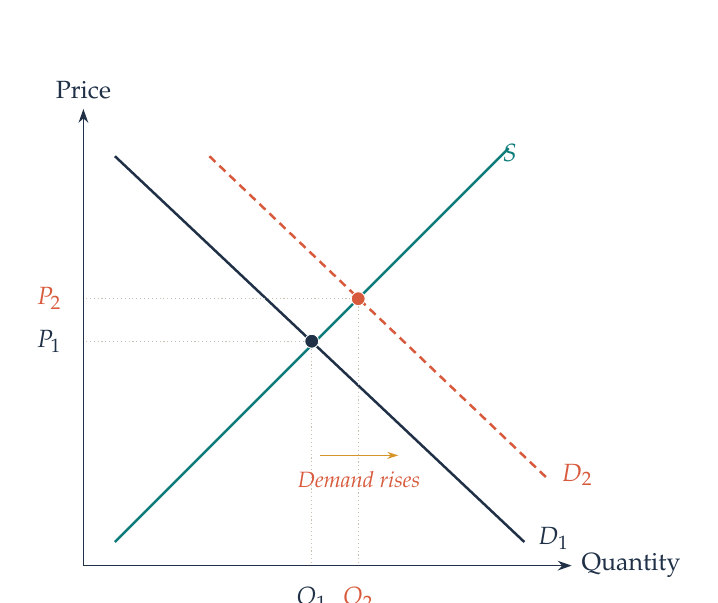
\begin{tikzpicture}[scale=1.0, baseline=(current bounding box.center)]
  % Axes
  \draw[econ axis] (0,0) -- (6.2,0) node[axis label, right] {Quantity};
  \draw[econ axis] (0,0) -- (0,5.8) node[axis label, above] {Price};

  % Supply curve
  \draw[curve C] (0.4,0.3) -- (5.4,5.3);
  \node[curve label, color=CurveSage, anchor=south west] at (5.2,5.0) {$S$};

  % Demand curve D1
  \draw[curve A] (0.4,5.2) -- (5.6,0.3);
  \node[curve label, color=CurveNavy, anchor=west] at (5.65,0.35) {$D_1$};

  % Demand curve D2 (shifted right)
  \draw[curve B shift] (1.6,5.2) -- (5.9,1.1);
  \node[curve label, color=CurveRose, anchor=west] at (5.95,1.15) {$D_2$};

  % Equilibrium 1 -- projection lines
  \draw[guide line] (2.9,2.85) -- (2.9,0);
  \draw[guide line] (2.9,2.85) -- (0,2.85);
  \node[tick label, below] at (2.9,-0.15) {$Q_1$};
  \node[tick label, left] at (-0.15,2.85) {$P_1$};
  \node[econ point] at (2.9,2.85) {};

  % Equilibrium 2 -- projection lines
  % S ∩ D2: x−0.1 = −0.9535x+6.726 → x=3.49, y=3.39
  \draw[guide line] (3.49,3.39) -- (3.49,0);
  \draw[guide line] (3.49,3.39) -- (0,3.39);
  \node[tick label, color=CurveRose, below] at (3.49,-0.15) {$Q_2$};
  \node[tick label, color=CurveRose, left] at (-0.15,3.39) {$P_2$};
  \node[econ point accent] at (3.49,3.39) {};

  % Shift arrow
  \draw[shift arrow] (3.0,1.4) -- (4.0,1.4);
  \node[annot accent, below] at (3.5,1.32) {Demand rises};
\end{tikzpicture}%
}{%
\textbf{\color{CurveNavy}How it works:}\\[7pt]
\textbf{1.}~Demand rises (D shifts to $D_2$)\\[4pt]
\textbf{2.}~Price rises from $P_1$ to $P_2$\\[4pt]
\textbf{\color{CurveSage}Signal:} \enspace``Produce more of this!''\\[4pt]
\textbf{\color{CurveSage}Incentive:} \enspace Higher profit attracts new suppliers\\[4pt]
\textbf{\color{CurveSage}Rationing:}\\[2pt]
Higher price limits consumption\\[2pt]
to those who value it most.%
}
\end{diagrambox}

\subsection{Advantages and Disadvantages of Each System}

\begin{longtable}{@{}>{\RaggedRight\arraybackslash}p{0.22\linewidth}>{\RaggedRight\arraybackslash}p{0.37\linewidth}>{\RaggedRight\arraybackslash}p{0.37\linewidth}@{}}
\rowcolor{NavyPrimary}
\textbf{\color{white}System} & \textbf{\color{white}Advantages} & \textbf{\color{white}Disadvantages} \\
\midrule
\endhead

\textbf{Market Economy}
\newline{\footnotesize e.g.\ USA, Hong Kong}
&
\begin{itemize}[leftmargin=*, topsep=0pt, itemsep=1pt]
  \item \textbf{Efficiency:} Competition and profit incentivise firms to minimise costs.
  \item \textbf{Consumer sovereignty:} Production responds to preferences.
  \item \textbf{Innovation:} Profit rewards risk-taking and new products.
  \item \textbf{Automatic adjustment:} No bureaucracy needed.
\end{itemize}
&
\begin{itemize}[leftmargin=*, topsep=0pt, itemsep=1pt]
  \item \textbf{Market failure:} Ignores public goods, demerit goods, externalities.
  \item \textbf{Inequality:} Resources flow to those who already own them.
  \item \textbf{Monopoly power:} Can lead to exploitation of consumers.
  \item \textbf{Macroeconomic instability:} Prone to booms and recessions.
\end{itemize}
\\
\midrule
\rowcolor{LightBlue}
\textbf{Planned Economy}
\newline{\footnotesize e.g.\ North Korea, former USSR}
&
\begin{itemize}[leftmargin=*, topsep=0pt, itemsep=1pt]
  \item \textbf{National goals:} Can direct resources to specific objectives.
  \item \textbf{Low unemployment:} The state can provide jobs for all.
  \item \textbf{Reduced inequality:} Controls wages and prices.
  \item \textbf{Avoids market failures:} Can provide public goods directly.
\end{itemize}
&
\begin{itemize}[leftmargin=*, topsep=0pt, itemsep=1pt]
  \item \textbf{Inefficiency:} No profit motive leads to low productivity and shortages.
  \item \textbf{Bureaucracy:} Central planning is slow and inflexible.
  \item \textbf{Lack of choice:} Consumer sovereignty is replaced by state sovereignty.
  \item \textbf{Corruption:} Concentrated power invites corruption.
\end{itemize}
\\
\midrule
\textbf{Mixed Economy}
\newline{\footnotesize e.g.\ UK, Germany, Sweden}
&
\begin{itemize}[leftmargin=*, topsep=0pt, itemsep=1pt]
  \item \textbf{Best of both worlds:} Efficiency of markets with correction of their failures.
  \item \textbf{Welfare provision:} Healthcare, education, safety nets.
  \item \textbf{Regulation:} Controls monopolies and negative externalities.
  \item \textbf{Greater equity:} Progressive taxes and benefits.
\end{itemize}
&
\begin{itemize}[leftmargin=*, topsep=0pt, itemsep=1pt]
  \item \textbf{Government failure:} Intervention can be inefficient or politically motivated.
  \item \textbf{Conflicting objectives:} Efficiency and equity goals often conflict.
  \item \textbf{Bureaucracy:} Can still suffer bureaucratic inefficiency.
\end{itemize}
\\
\caption{Comparison of Economic Systems}
\end{longtable}

\begin{evaluation}{Market, Planned, and Mixed Economies}
\textbf{Strengths of Market Economies:}
\begin{itemize}[leftmargin=*, nosep]
\item Allocative efficiency through price signals — firms respond to consumer preferences without central coordination.
\item Dynamic efficiency — profit incentives drive innovation and technological progress.
\item Rapid adaptation to changing circumstances — no bureaucratic delays.
\end{itemize}

\textbf{Strengths of Planned/Command Systems:}
\begin{itemize}[leftmargin=*, nosep]
\item Guaranteed provision of public goods (defence, infrastructure) that markets underproduce.
\item Can prioritise equity — direct redistribution without relying on market mechanisms.
\item Eliminates unemployment through job guarantees (in theory).
\end{itemize}

\textbf{Limitations — Why Pure Systems Rarely Exist:}
\begin{itemize}[leftmargin=*, nosep]
\item \textbf{Market failure:} Pure markets fail to provide public goods, control externalities, or prevent monopolies. This necessitates government intervention.
\item \textbf{Government failure:} Central planning suffers from information asymmetry, slow decision-making, and corruption. Planners cannot replicate the distributed knowledge embedded in market prices.
\item \textbf{Equity-efficiency trade-off:} Redistribution to achieve equity often reduces efficiency through reduced work and investment incentives.
\end{itemize}

\textbf{It depends on\ldots}
\begin{itemize}[leftmargin=*, nosep]
\item \textbf{Type of good:} Public goods (defence, roads) suit state provision; personal services suit markets.
\item \textbf{Extent of market failure:} How severe are externalities, monopoly power, and information asymmetries? The worse the market failure, the stronger the case for intervention.
\item \textbf{Government capability:} Can the state realistically implement intervention? Regulatory capacity, corruption levels, and bureaucratic efficiency all matter.
\item \textbf{Values and priorities:} Different societies weigh efficiency and equity differently. Scandinavian countries choose high taxes for welfare; the US prioritises lower taxes and market freedom.
\end{itemize}
\end{evaluation}

% ── Production Possibility Curves ────────────────────────────
\section{Production Possibility Curves}



\subsection{Nature and Meaning of a Production Possibility Curve}

\begin{keyterm}{Production Possibility Curve (PPC)}
A \textbf{PPC} shows the maximum potential combinations of two goods or services that an economy can achieve when \emph{all} its resources are \textbf{fully and efficiently employed}, using a given level of technology.
\end{keyterm}

The PPC is one of economics' most powerful visual tools. It demonstrates three core ideas simultaneously:
\begin{itemize}
  \item \textbf{Scarcity:} You cannot produce beyond the curve with current resources.
  \item \textbf{Choice:} You must select a point on the curve -- you cannot have everything.
  \item \textbf{Opportunity cost:} Moving along the curve to produce more of one good means sacrificing some of the other.
\end{itemize}

\subsection{Shape of the PPC: Constant vs. Increasing Opportunity Cost}

\subsubsection{The Curved PPC (Increasing Opportunity Cost)}

\begin{coreidea}
The standard PPC is \textbf{concave to the origin} (bowed outward). This shape reflects \emph{increasing opportunity cost}: as you produce more of Good X, you must sacrifice ever-increasing amounts of Good Y.
\end{coreidea}

\textbf{Why?} Resources are not perfectly adaptable between uses. Consider an economy producing both dairy goods and military weapons. At first, the government reassigns engineers and mechanics -- workers already suited to weapon-making -- and the gain in guns is large relative to the loss in dairy output. But as production of weapons expands, all engineers have already been moved. The next workers available are dairy farmers. Reassigning a dairy farmer to a weapons factory causes a \emph{large} loss in dairy output but only a \emph{small} gain in weapons, because the farmer's skills lie in milk production, not precision engineering.

The more you reallocate resources, the greater the productive capacity you sacrifice in the original sector relative to what you gain in the new one. This is why the PPC bows outward: each additional unit of guns costs an ever-increasing amount of dairy output.

\begin{diagrambox}[Figure II -- Curved PPC: Increasing Opportunity Cost]
\diagramwithtext{%
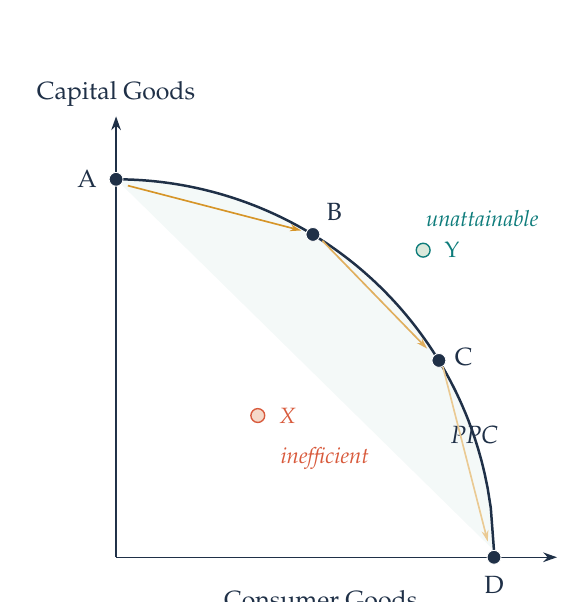
\begin{tikzpicture}[scale=1.0, baseline=(current bounding box.center)]
  % Axes
  \draw[econ axis] (0,0) -- (5.6,0);
  \draw[econ axis] (0,0) -- (0,5.6) node[axis label, above] {Capital Goods};
  \node[axis label, below] at (2.6,-0.3) {Consumer Goods};

  % Subtle fill under PPC
  \begin{scope}
    \clip (0,0) -- plot[domain=0:4.8, samples=100] (\x, {sqrt(23.04 - \x*\x)}) -- (0,4.8) -- cycle;
    \fill[FillPrimary, opacity=0.25] (0,0) rectangle (4.8,4.8);
  \end{scope}

  % Curved PPC
  \draw[curve A, domain=0:4.8, samples=120]
        plot (\x, {sqrt(23.04 - \x*\x)});
  \node[curve label, color=CurveNavy] at (4.55, 1.55) {PPC};

  % Points A--D on the curve
  \node[econ point] (ptA) at (0,4.8) {};
  \node[axis label, left, font=\small] at (-0.12,4.8) {A};
  \node[econ point] (ptB) at (2.5,4.1) {};
  \node[axis label, above right, font=\small] at (2.55,4.15) {B};
  % PPC: y=√(23.04−x²). At x=4.1: y=√(23.04−16.81)=√6.23=2.496≈2.50
  \node[econ point] (ptC) at (4.1,2.50) {};
  \node[axis label, right, font=\small] at (4.18,2.55) {C};
  \node[econ point] (ptD) at (4.8,0) {};
  \node[axis label, below, font=\small] at (4.8,-0.12) {D};

  % Point inside (inefficient)
  \node[econ point open, draw=CurveRose, fill=FillSecondary] at (1.8,1.8) {};
  \node[annot accent, right] at (1.95,1.8) {X};
  \node[annot, color=CurveRose, font=\footnotesize\itshape] at (2.65,1.25) {inefficient};

  % Point outside (unattainable)
  \node[econ point open, draw=CurveSage, fill=FillPositive] at (3.9,3.9) {};
  \node[annot, color=CurveSage, right, font=\footnotesize] at (4.05,3.9) {Y};
  \node[annot, color=CurveSage, font=\footnotesize\itshape] at (4.65,4.3) {unattainable};

  % Increasing OC arrows (progressively lighter to show increasing cost)
  \draw[shift arrow, color=CurveGold] (0.15,4.72) -- (2.35,4.15);
  \draw[shift arrow, color=CurveGold!75] (2.62,4.02) -- (3.95,2.65);
  \draw[shift arrow, color=CurveGold!50] (4.15,2.42) -- (4.72,0.2);
\end{tikzpicture}%
}{%
\textbf{\color{CurveNavy}Reading the diagram:}\\[7pt]
\textbf{Points A--D} lie on the PPC\enspace$\rightarrow$\enspace productively efficient.\\[5pt]
\textbf{Point X} lies inside\enspace$\rightarrow$\enspace inefficient (idle resources).\\[5pt]
\textbf{Point Y} lies outside\enspace$\rightarrow$\enspace currently unattainable.\\[10pt]
\textbf{\color{CurveGold}Increasing opportunity cost:} The arrows A$\,\to\,$B, B$\,\to\,$C, C$\,\to\,$D each represent the same gain in Consumer Goods, but each requires a \emph{larger} sacrifice of Capital Goods.%
}
\end{diagrambox}

\subsubsection{The Straight-Line PPC (Constant Opportunity Cost)}

A straight PPC implies \emph{constant opportunity cost} -- the same amount of Good Y is always sacrificed for each additional unit of Good X. This assumes resources are perfectly adaptable between the two uses.

\begin{diagrambox}[Figure IIb -- Straight-Line PPC: Constant Opportunity Cost]
\diagramwithtext{%
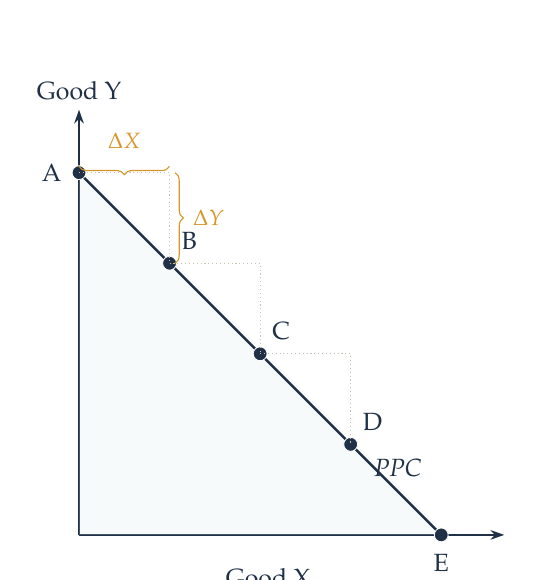
\begin{tikzpicture}[scale=1.0, baseline=(current bounding box.center)]
  % Axes
  \draw[econ axis] (0,0) -- (5.4,0);
  \draw[econ axis] (0,0) -- (0,5.4) node[axis label, above] {Good Y};
  \node[axis label, below] at (2.4,-0.3) {Good X};

  % Subtle fill under PPC
  \fill[FillPrimary, opacity=0.2] (0,0) -- (0,4.6) -- (4.6,0) -- cycle;

  % Straight PPC
  \draw[curve A] (0,4.6) -- (4.6,0);
  \node[curve label, color=CurveNavy] at (4.05, 0.85) {PPC};

  % Equal-sized steps along the PPC
  \node[econ point] at (0,4.6) {};
  \node[axis label, left, font=\small] at (-0.1,4.6) {A};
  \node[econ point] at (1.15,3.45) {};
  \node[axis label, above right, font=\small] at (1.18,3.5) {B};
  \node[econ point] at (2.3,2.3) {};
  \node[axis label, above right, font=\small] at (2.33,2.35) {C};
  \node[econ point] at (3.45,1.15) {};
  \node[axis label, above right, font=\small] at (3.48,1.2) {D};
  \node[econ point] at (4.6,0) {};
  \node[axis label, below, font=\small] at (4.6,-0.12) {E};

  % Step lines showing equal sacrifice
  \draw[guide line] (0,4.6) -- (1.15,4.6) -- (1.15,3.45);
  \draw[guide line] (1.15,3.45) -- (2.3,3.45) -- (2.3,2.3);
  \draw[guide line] (2.3,2.3) -- (3.45,2.3) -- (3.45,1.15);

  % Dimension labels with braces
  \draw[decorate, decoration={brace, amplitude=3pt, mirror}, color=CurveGold, line width=0.4pt]
    (0,4.68) -- (1.15,4.68) node[midway, above=3pt, annot, color=CurveGold] {$\Delta X$};
  \draw[decorate, decoration={brace, amplitude=3pt}, color=CurveGold, line width=0.4pt]
    (1.22,4.6) -- (1.22,3.45) node[midway, right=3pt, annot, color=CurveGold] {$\Delta Y$};
\end{tikzpicture}%
}{%
\textbf{\color{CurveNavy}Constant opportunity cost:}\\[7pt]
Every equal step along the X-axis (A$\,\to\,$B$\,\to\,$C$\,\to\,$D$\,\to\,$E) sacrifices exactly the same amount of Good~Y.\\[9pt]
\textbf{Why constant?} Resources are assumed to be \emph{perfectly adaptable} between uses --- a worker can switch between goods with no loss of productivity.\\[9pt]
{\color{AnnotGray}\itshape Note:\enspace This is a simplifying assumption. In reality, the curved PPC is more realistic.}%
}
\end{diagrambox}

\subsection{Shifts in the PPC}

A shift in the PPC occurs when there is a change in the \emph{quantity} or \emph{quality} of resources, or in technology.

\subsubsection{Outward Shift -- Economic Growth}

\begin{diagrambox}[Figure III -- Outward Shift of the PPC (Economic Growth)]
\diagramwithtext{%
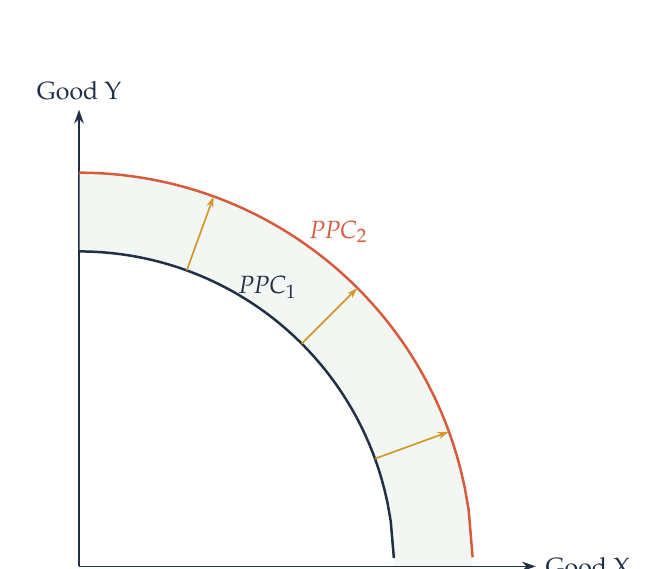
\begin{tikzpicture}[scale=1.0, baseline=(current bounding box.center)]
  % Axes
  \draw[econ axis] (0,0) -- (5.8,0) node[axis label, right] {Good X};
  \draw[econ axis] (0,0) -- (0,5.8) node[axis label, above] {Good Y};

  % Subtle fill between the two PPCs to show the expansion zone
  \begin{scope}
    \clip plot[domain=0:4.0, samples=80] (\x, {sqrt(16 - \x*\x)}) -- (4.0,0) -- (5.0,0) --
          plot[domain=5.0:0, samples=80] (\x, {sqrt(25 - \x*\x)}) -- cycle;
    \fill[FillPositive, opacity=0.35] (0,0) rectangle (5.0,5.0);
  \end{scope}

  % Original PPC
  \draw[curve A, domain=0:4.0, samples=100]
        plot (\x, {sqrt(16 - \x*\x)});
  \node[curve label, color=CurveNavy] at (2.4, 3.55) {$\textit{PPC}_1$};

  % New PPC (outward)
  \draw[curve B, domain=0:5.0, samples=100]
        plot (\x, {sqrt(25 - \x*\x)});
  \node[curve label, color=CurveRose] at (3.3, 4.25) {$\textit{PPC}_2$};

  % Elegant outward arrows
  \foreach \a in {20,45,70} {
    \pgfmathsetmacro{\xone}{4.0 * cos(\a)}
    \pgfmathsetmacro{\yone}{4.0 * sin(\a)}
    \pgfmathsetmacro{\xtwo}{5.0 * cos(\a)}
    \pgfmathsetmacro{\ytwo}{5.0 * sin(\a)}
    \draw[shift arrow] (\xone, \yone) -- (\xtwo, \ytwo);
  }
\end{tikzpicture}%
}{%
\textbf{\color{CurveNavy}Causes of outward shift:}\\[6pt]
{\small%
\hangindent=1em\hangafter=1 \textcolor{CurveGold}{$\circ$}\enspace Discovery of new natural resources\\[3pt]
\hangindent=1em\hangafter=1 \textcolor{CurveGold}{$\circ$}\enspace Growth in the labour force (e.g.\ immigration)\\[3pt]
\hangindent=1em\hangafter=1 \textcolor{CurveGold}{$\circ$}\enspace Investment in new capital machinery\\[3pt]
\hangindent=1em\hangafter=1 \textcolor{CurveGold}{$\circ$}\enspace Improvements in education \& training (human capital)\\[3pt]
\hangindent=1em\hangafter=1 \textcolor{CurveGold}{$\circ$}\enspace Technological innovation}\\[10pt]
\textbf{\color{CurveGold}Consequence:}\enspace economy can produce more of \emph{both} goods --- higher living standards possible.%
}
\end{diagrambox}

\subsubsection{Inward Shift -- Economic Decline}

An inward shift (PPC moves toward the origin) means reduced productive capacity. Causes include natural disasters, wars that destroy capital, or the depletion of essential resources without a substitute.

\begin{tcolorbox}[
  enhanced, colback=LightGold, colframe=GoldAccent,
  arc=0pt, boxrule=0.7pt,
  left=8pt, right=8pt, top=6pt, bottom=6pt
]
\textbf{\color{NavyPrimary}Important distinction:} A \emph{recession} (fall in aggregate demand) does \textbf{not} shift the PPC inward. It moves the economy from a point \emph{on} the curve to a point \emph{inside} it (point X in Figure II above). The productive capacity remains -- it is just not being used.
\end{tcolorbox}

\subsection{Points Inside the PPC -- Inefficiency}

A point \emph{inside} the PPC signals that resources are being wasted. Possible causes:

\begin{itemize}
  \item \textbf{Unemployment:} Labour and capital are sitting idle.
  \item \textbf{Underemployment:} Resources are being used below their potential (e.g., a surgeon working as a hospital porter).
  \item \textbf{Inefficient production:} Outdated technology or poor management wasting inputs.
\end{itemize}

\textbf{Moving back to the PPC} (without new resources) requires better resource allocation. Policy options include:
\begin{itemize}
  \item Fiscal or monetary stimulus to boost aggregate demand and reduce cyclical unemployment.
  \item Training programmes and job-matching services to reduce structural/frictional unemployment.
  \item Deregulation and competition policy to improve productive efficiency.
\end{itemize}

\begin{evaluation}{Production Possibility Curves and Opportunity Cost}
\textbf{Strengths / Why PPCs Are Central to Economics:}
\begin{itemize}[leftmargin=*, nosep]
\item Visually encapsulates three core concepts simultaneously: scarcity, choice, and opportunity cost.
\item Shows that efficiency is not just about minimising cost — it also requires producing at the \emph{right} mix of goods (allocative efficiency).
\item Economic growth is clearly defined: outward shift of the PPC, not just movement along it.
\item Illustrates why different countries have different PPCs due to endowments, technology, and specialisation patterns.
\end{itemize}

\textbf{Limitations and Critiques:}
\begin{itemize}[leftmargin=*, nosep]
\item Assumes only two goods — real economies produce thousands. Multi-dimensional PPCs become intractable to visualize.
\item Assumes fixed technology and resource quality. In reality, technology evolves dynamically, and discovery of new resources is common.
\item Does not account for environmental degradation — producing more of Good X may degrade the natural capital needed for Good Y, shifting the PPC inward in ways the standard model ignores.
\item Assumes full employment. In reality, the economy often sits inside the PPC due to cyclical unemployment — but distinguishing between cyclical and structural causes requires deeper macroeconomic analysis.
\end{itemize}

\textbf{It depends on\ldots}
\begin{itemize}[leftmargin=*, nosep]
\item \textbf{Time horizon:} Short run — the PPC is fixed, so opportunity cost is constant. Long run — growth and technological change shift the PPC, creating new opportunities.
\item \textbf{Whether goods are substitutes or complements in production:} A straight PPC assumes perfect substitution. In reality, shared resources (e.g., a factory that can produce either cars or trucks) create a straight-line trade-off, while completely independent productions (e.g., fish and forestry on different terrain) may have a more curved profile.
\item \textbf{Extent of market failure:} If markets function well, the economy gravitates toward the PPC. If monopolies, externalities, or information failures abound, the economy may remain persistently inside.
\end{itemize}
\end{evaluation}

% ── Classification of Goods and Services ─────────────────────
\section{Classification of Goods and Services}



\subsection{Free Goods vs. Private Goods}

\begin{keyterm}{Free Good}
A good that is \textbf{not scarce} relative to demand. It is available in abundance at zero price and has \textbf{zero opportunity cost} -- one person's use does not prevent another's. Example: air, sunlight, seawater.
\end{keyterm}

\begin{keyterm}{Private Good (Economic Good)}
A good that \textbf{is scarce} relative to demand. It has an opportunity cost and must be produced using resources that have alternative uses. The vast majority of goods are private goods.
\end{keyterm}

\subsubsection{Excludability and Rivalry}

These two properties are the foundation for classifying all goods:

\begin{tcolorbox}[
  enhanced, colback=LightBlue, colframe=NavyPrimary,
  arc=0pt, boxrule=0.7pt
]
\begin{tabular}{@{}>{\RaggedRight\arraybackslash}p{0.22\linewidth}>{\RaggedRight\arraybackslash}p{0.37\linewidth}>{\RaggedRight\arraybackslash}p{0.37\linewidth}@{}}
& \textbf{\color{NavyPrimary}Excludable} & \textbf{\color{NavyPrimary}Non-Excludable} \\
\midrule
\textbf{Rival} & \textbf{Private good} \newline (e.g. a sandwich, a car) & \textbf{Common resource} \newline (e.g. fish in the sea) \\
\addlinespace
\textbf{Non-Rival} & \textbf{Club good} \newline (e.g. a toll road, Netflix) & \textbf{Pure public good} \newline (e.g. national defence, street lighting) \\
\end{tabular}
\end{tcolorbox}

\subsection{Public Goods}

\begin{keyterm}{Public Good}
A good that is \textbf{non-excludable} (impossible to prevent non-payers from benefiting) \textbf{and non-rival} (one person's consumption does not diminish supply for others).
\end{keyterm}

\subsubsection{The Free Rider Problem}

\begin{coreidea}
Because public goods are non-excludable, individuals can consume them without paying. This creates the \textbf{free rider problem}: private firms cannot charge a price, so they have no incentive to supply the good. Without government provision, public goods would be \emph{under-provided or not provided at all}.
\end{coreidea}

\textbf{Solution:} The government provides public goods and finances them through \emph{compulsory taxation}, overcoming the free rider problem.

\subsubsection{Quasi-Public Goods}

Some goods have characteristics of \emph{both} public and private goods. These are \textbf{quasi-public goods}:

\begin{itemize}
  \item \textbf{Roads:} Non-excludable normally, but become \emph{rival} during rush-hour congestion, and can be made excludable with toll charges.
  \item \textbf{Public parks:} Non-excludable normally, but can become crowded (rival) and can be gated at night (excludable).
  \item \textbf{The internet:} Non-rival (your browsing doesn't slow mine), but easily made excludable via passwords and subscriptions.
\end{itemize}

\subsection{Merit Goods}

\begin{keyterm}{Merit Good}
A good that the government believes is \textbf{under-consumed} in a free market due to \textbf{imperfect information}. The government encourages consumption because it generates positive benefits for both the individual and society.
\end{keyterm}

\subsubsection{Why Are Merit Goods Under-Consumed?}

Consumers may \emph{not fully understand} the long-term private benefits or the positive externalities of the good (that is, the wider benefits their consumption brings to society as a whole). They may be short-sighted (preferring instant gratification) or simply unaware of the full benefits. As a result, they demand \emph{less} than is socially optimal.

\begin{example}[Merit Goods in Practice]
\begin{itemize}
  \item \textbf{Education:} Individuals may undervalue the lifelong earnings benefit and the social benefit of a more productive, innovative, and law-abiding citizenry.
  \item \textbf{Vaccinations:} A person may ignore the herd immunity benefit to society -- only seeing their own small individual gain.
  \item \textbf{Museums and libraries:} Individuals may not appreciate the broader cultural and educational benefits.
\end{itemize}
\end{example}

\subsection{Demerit Goods}

\begin{keyterm}{Demerit Good}
A good that the government believes is \textbf{over-consumed} in a free market due to \textbf{imperfect information}. The government discourages consumption because it has negative consequences for both the individual and society.
\end{keyterm}

\subsubsection{Why Are Demerit Goods Over-Consumed?}

Consumers \emph{underestimate} the long-term harm to themselves and the negative externalities imposed on others. They may be addicted (and thus unable to make fully rational choices), ignorant of the true risks, or simply discount future costs.

\begin{example}[Demerit Goods in Practice]
\begin{itemize}
  \item \textbf{Cigarettes:} Smokers underestimate cancer risk; smoking also creates negative externalities (passive smoking, public healthcare costs).
  \item \textbf{Alcohol:} Consumers underappreciate health risks and social costs (accidents, crime, domestic violence).
  \item \textbf{Illegal drugs:} High potential for addiction; enormous social costs including crime and family breakdown.
  \item \textbf{High-sugar/fatty foods:} Consumers ignore long-term health consequences (obesity, diabetes) that impose costs on public health systems.
\end{itemize}
\end{example}

\subsubsection{Summary: Merit vs. Demerit Goods}

\begin{tcolorbox}[
  enhanced, colback=LightBlue, colframe=NavyPrimary,
  arc=0pt, boxrule=0.7pt
]
\begin{tabular}{@{}>{\RaggedRight\arraybackslash}p{0.22\linewidth}>{\RaggedRight\arraybackslash}p{0.37\linewidth}>{\RaggedRight\arraybackslash}p{0.37\linewidth}@{}}
& \textbf{\color{NavyPrimary}Merit Good} & \textbf{\color{NavyPrimary}Demerit Good} \\
\midrule
\textbf{Free market outcome} & Under-consumed & Over-consumed \\
\textbf{Information problem} & Consumers underestimate benefits & Consumers underestimate costs \\
\textbf{Government response} & Subsidise; provide free; compulsory & Tax; ban; restrict; regulate \\
\textbf{Examples} & Education, healthcare, vaccinations & Cigarettes, alcohol, illegal drugs \\
\end{tabular}
\end{tcolorbox}

\begin{evaluation}{Classification of Goods: Public/Private, Merit/Demerit}
\textbf{Strengths of This Classification:}
\begin{itemize}[leftmargin=*, nosep]
\item Explains why the free market fails to allocate efficiently for certain goods — essential for understanding when government intervention is justified.
\item Merit goods highlight the limits of consumer sovereignty when imperfect information distorts demand.
\item Helps distinguish between different types of government failure: a public good justifies state provision; a merit good justifies subsidies or compulsory provision; a demerit good justifies taxation or restriction.
\end{itemize}

\textbf{Limitations:}
\begin{itemize}[leftmargin=*, nosep]
\item \textbf{Classification is normative:} Whether a good is "merit" or "demerit" depends on government values. What one government deems meritorious, another may not (e.g., abortion, contraception).
\item \textbf{Private benefits vs. social benefits blur:} Education is classified as a merit good because of presumed underestimation of benefits. But if a person highly values education for themselves alone, they are not making an irrational choice — they simply weight private benefit differently than the government thinks they should.
\item \textbf{Information asymmetry is often exaggerated:} Modern consumers have access to vast information (health websites, product reviews, research articles). Whether they choose to process this information is a matter of preference, not ignorance.
\item \textbf{Behavioural assumptions:} The classification assumes consumers are myopic or irrational. But revealed preference theory suggests that people's actual choices reflect their true preferences — if people under-consume education, it may be because they rationally discount future benefits or prioritise present consumption.
\end{itemize}

\textbf{It depends on\ldots}
\begin{itemize}[leftmargin=*, nosep]
\item \textbf{Availability of information:} In the age of the internet, whether consumers genuinely lack information about education's benefits is debatable. This undermines the rationale for mandatory schooling laws.
\item \textbf{Non-excludability of benefits:} If the social benefit of your education accrues mainly to you (higher salary, career satisfaction), then subsidy is harder to justify than if it accrues broadly to society (herd immunity from vaccinations).
\item \textbf{Severity of the market failure:} Modest information gaps justify subsidies and advisory programmes. Severe ones (e.g., highly addictive substances) justify taxation or restriction.
\item \textbf{Government capacity to intervene wisely:} Even if a good is merit or demerit, government may lack the expertise to decide the "right" level of consumption. State provision of education works well in many countries; state provision of entertainment or dating services would be absurd.
\end{itemize}
\end{evaluation}

\section{Exam Practice Questions -- Chapter 1}

\begin{exampractice}
\begin{enumerate}[leftmargin=*]

\item \textbf{``Evaluate the claim that a mixed economy is always superior to either a pure market or a pure planned economy.''} [15 marks]

\textit{Model structure: Define market, planned, and mixed economies $\to$ Compare on grounds of efficiency, equity, innovation, and responsiveness $\to$ Assess the claim with reference to different contexts (healthcare vs. luxury goods) and different priorities (poverty reduction vs. growth) $\to$ Conclude with `it depends on social values and market conditions'.}

\item \textbf{``To what extent is opportunity cost a more useful concept than comparative advantage for understanding why countries specialise in production?''} [15 marks]

\textit{Model structure: Define both concepts $\to$ Show how opportunity cost explains specialisation $\to$ Explain comparative advantage (and how it relies on opportunity cost) $\to$ Discuss transaction costs, externalities, and political economy that the models ignore $\to$ Conclude on practical usefulness.}

\item \textbf{``Using a PPC diagram, explain how economic growth differs from a recession, and discuss whether governments can always return the economy to the PPC without generating inflation.''} [15 marks]

\textit{Model structure: Draw PPC; show recession as movement inside $\to$ show growth as outward shift $\to$ Discuss fiscal/monetary stimulus mechanisms $\to$ Explain demand-pull inflation when stimulus is too large $\to$ Distinguish between moving back to PPC (counter-cyclical policy) and shifting the PPC itself (supply-side policy) $\to$ Evaluate the time lag and political economy of stimulus packages.}

\item \textbf{``How do merit goods and demerit goods justify government intervention despite the efficiency properties of competitive markets?''} [15 marks]

\textit{Model structure: Define merit/demerit goods $\to$ Explain information failure and its welfare consequences $\to$ Show why the free market outcome is not Pareto optimal $\to$ Discuss government intervention tools (subsidies for merit goods, taxes/bans for demerit goods) $\to$ Evaluate the paternalism objection: to what extent should governments override individual choice? $\to$ Conclude: it depends on severity of information failure and government's comparative advantage in judging welfare.}

\end{enumerate}
\end{exampractice}

% ============================================================
%  CHAPTER 2: THE PRICE SYSTEM AND THE MICROECONOMY
% ============================================================
\chapter{The Price System and the Microeconomy}

\section{Demand and Supply Curves}



\subsection{Effective Demand and the Price Mechanism}

\begin{keyterm}{Effective Demand}
\textbf{Effective demand} is the desire for a good backed by the \emph{ability and willingness to pay}. A mere wish to own a Ferrari is notional demand; only if you can afford to buy one does it become effective demand that influences the market.
\end{keyterm}

\begin{keyterm}{Market}
Any \textbf{arrangement} that brings buyers and sellers together to exchange goods and services. It does not have to be a physical location -- stock markets, online platforms (eBay), and local shops are all markets.
\end{keyterm}

The price mechanism allocates resources through three interlocking functions:
\begin{itemize}
  \item \textbf{Signalling:} High prices signal scarcity and profitability; low prices signal a surplus.
  \item \textbf{Incentive:} The prospect of profit motivates firms to increase supply.
  \item \textbf{Rationing:} Rising prices ration scarce goods to those willing and able to pay the most.
\end{itemize}

\subsection{The Demand Curve}

\begin{keyterm}{Demand Curve}
A curve showing the \textbf{relationship between the price of a good and the quantity demanded}, \emph{ceteris paribus}. It is almost always \textbf{downward-sloping}.
\end{keyterm}

The demand curve slopes downward for two reasons:
\begin{itemize}
  \item \textbf{Income effect:} A lower price raises your real purchasing power, so you buy more.
  \item \textbf{Substitution effect:} As a good becomes cheaper relative to alternatives, consumers switch towards it.
\end{itemize}

The \textbf{market demand curve} is the \emph{horizontal sum} of all individual demand curves -- at each price, we add up every consumer's quantity demanded.

\subsection{The Supply Curve}

\begin{keyterm}{Supply Curve}
A curve showing the \textbf{relationship between the price of a good and the quantity supplied}, \emph{ceteris paribus}. It is usually \textbf{upward-sloping}.
\end{keyterm}

The supply curve slopes upward because a higher price makes production more profitable, incentivising firms to produce and sell more. Higher prices may also cover the rising marginal costs of producing additional units (e.g.\ overtime wages).

The \textbf{market supply curve} is the \emph{horizontal sum} of all individual firms' supply curves.

\subsection{Movements Along vs.\ Shifts of the Curve}

\begin{coreidea}
This is the single most important distinction in demand and supply analysis. A change in the good's \emph{own price} causes a \textbf{movement along} the curve. A change in \emph{any other determinant} causes the \emph{entire curve to shift}.
\end{coreidea}

\begin{diagrambox}[Figure IV -- Movement Along vs.\ Shift of the Demand Curve]
\diagramwithtext{%
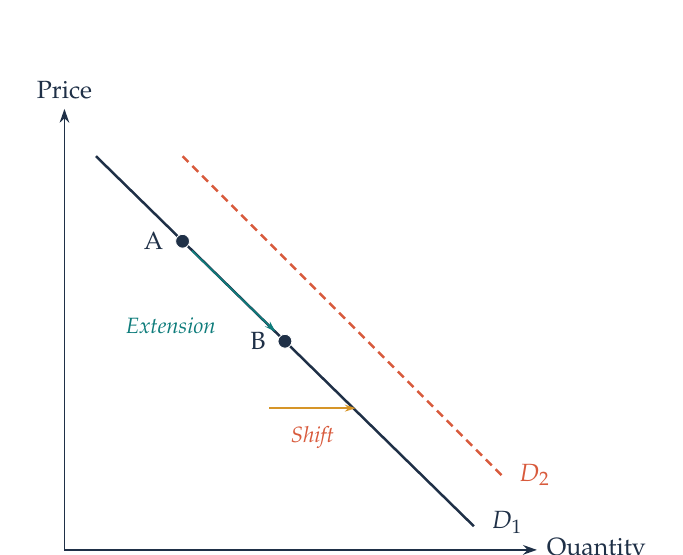
\begin{tikzpicture}[scale=1.0, baseline=(current bounding box.center)]
  % Axes
  \draw[econ axis] (0,0)--(6.0,0) node[axis label, right]{Quantity};
  \draw[econ axis] (0,0)--(0,5.6) node[axis label, above]{Price};

  % Original demand D1
  \draw[curve A] (0.4,5.0)--(5.2,0.3);
  \node[curve label, color=CurveNavy, anchor=west] at (5.3,0.35) {$D_1$};

  % Points A and B on D1 (movement along curve)
  % D1: (0.4,5.0)→(5.2,0.3), slope=−0.9792. At x=1.5: y=3.92. At x=2.8: y=2.65
  \node[econ point] at (1.5,3.92) {};
  \node[axis label, left, font=\small] at (1.38,3.92) {A};
  \node[econ point] at (2.8,2.65) {};
  \node[axis label, left, font=\small] at (2.68,2.65) {B};
  \draw[shift arrow, color=CurveSage] (1.62,3.80)--(2.68,2.77);
  \node[annot, color=CurveSage, font=\footnotesize\itshape] at (1.35,2.85) {Extension};

  % Shifted demand D2
  \draw[curve B shift] (1.5,5.0)--(5.6,0.9);
  \node[curve label, color=CurveRose, anchor=west] at (5.65,0.95) {$D_2$};

  % Shift arrow
  \draw[shift arrow] (2.6,1.8)--(3.7,1.8);
  \node[annot accent, below] at (3.15,1.7) {Shift};
\end{tikzpicture}%
}{%
\textbf{\color{NavyPrimary}Reading the diagram:}\\[4pt]
\textbf{Movement Along the Curve (A $\to$ B):}\enspace A change in price causes \emph{extension} (quantity demanded increases) or \emph{contraction} (quantity demanded falls). The demand curve itself does not move -- we move along the same curve $D_1$.\\[6pt]
\textbf{Shift of the Curve ($D_1 \to D_2$):}\enspace A change in a non-price determinant (income, preferences, substitutes, etc.) causes the \emph{entire curve} to shift. At each price level, quantity demanded is now different. The curve position changes.\\[8pt]
\textbf{\color{GoldAccent}Key:}\enspace Own-price change $\Rightarrow$ movement along; other changes $\Rightarrow$ curve shifts.%
}
\end{diagrambox}

\subsection{Determinants of Demand (Causes of Curve Shifts)}

\begin{tcolorbox}[enhanced,colback=LightBlue,colframe=MidBlue!70,arc=0pt,boxrule=0.8pt]
\begin{tabular}{@{}>{\RaggedRight\arraybackslash}p{0.3\linewidth}>{\RaggedRight\arraybackslash}p{0.65\linewidth}@{}}
\textbf{\color{NavyPrimary}Determinant} & \textbf{\color{NavyPrimary}Effect on Demand} \\
\midrule
\textbf{Income (Normal Good)} & Income rises $\Rightarrow$ Demand increases (D shifts right). \\
\textbf{Income (Inferior Good)} & Income rises $\Rightarrow$ Demand decreases (D shifts left). \\
\textbf{Price of a Substitute} & Price of substitute rises $\Rightarrow$ Demand for this good increases. \\
\textbf{Price of a Complement} & Price of complement rises $\Rightarrow$ Demand for this good decreases. \\
\textbf{Tastes \& Fashion} & Positive trend $\Rightarrow$ Demand increases; negative trend $\Rightarrow$ Decreases. \\
\textbf{Population} & Larger population $\Rightarrow$ Greater market demand. \\
\textbf{Expectations} & Expected future price rise $\Rightarrow$ Demand increases now. \\
\end{tabular}
\end{tcolorbox}

\subsection{Determinants of Supply (Causes of Curve Shifts)}

\begin{tcolorbox}[enhanced,colback=LightBlue,colframe=MidBlue!70,arc=0pt,boxrule=0.8pt]
\begin{tabular}{@{}>{\RaggedRight\arraybackslash}p{0.3\linewidth}>{\RaggedRight\arraybackslash}p{0.65\linewidth}@{}}
\textbf{\color{NavyPrimary}Determinant} & \textbf{\color{NavyPrimary}Effect on Supply} \\
\midrule
\textbf{Costs of Production} & Costs rise $\Rightarrow$ Supply decreases (S shifts left). Most important determinant. \\
\textbf{Technology} & Improved technology $\Rightarrow$ Supply increases (S shifts right). \\
\textbf{Number of Firms} & More firms enter $\Rightarrow$ Market supply increases. \\
\textbf{Indirect Tax} & Tax imposed $\Rightarrow$ Costs rise, supply decreases. \\
\textbf{Government Subsidy} & Subsidy given $\Rightarrow$ Costs fall, supply increases. \\
\textbf{Price of Other Goods} & Price of alternative rises $\Rightarrow$ Firms switch; supply of this good falls. \\
\textbf{Weather (Agriculture)} & Bad weather $\Rightarrow$ Supply of crops decreases. \\
\end{tabular}
\end{tcolorbox}

\begin{tcolorbox}[enhanced,colback=LightGold,colframe=GoldAccent,arc=0pt,boxrule=0.9pt,
  left=8pt,right=8pt,top=6pt,bottom=6pt]
\textbf{\color{NavyPrimary}Critical Summary -- Movement vs.\ Shift:} A change in the good's \emph{own price} $\Rightarrow$ movement along the \emph{same} curve (extension/contraction). Any other change $\Rightarrow$ the \emph{entire curve} shifts to a new position (increase/decrease). Never confuse these two.
\end{tcolorbox}

% ── Elasticities of Demand ───────────────────────────────────
\section{Elasticities of Demand}



\subsection{Price Elasticity of Demand (PED)}

\begin{keyterm}{Price Elasticity of Demand (PED)}
A measure of the \textbf{responsiveness of quantity demanded} to a change in the good's own price, \emph{ceteris paribus}.
\[
\text{PED} = \frac{\%\;\Delta\text{Quantity Demanded}}{\%\;\Delta\text{Price}}
\]
PED is almost always \textbf{negative} (law of demand). We often refer to its \emph{absolute value}.
\end{keyterm}

\begin{example}[Calculating PED]
The price of a chocolate bar rises from \$1.00 to \$1.10 (+10\%). Quantity demanded falls from 100 to 88 bars ($-$12\%).
\[
\text{PED} = \frac{-12\%}{+10\%} = -1.2
\]
$|\text{PED}| = 1.2 > 1$, so demand is \textbf{price elastic}.
\end{example}

\subsubsection{Interpreting PED Values}

\begin{tcolorbox}[enhanced,colback=LightBlue,colframe=MidBlue!70,arc=0pt,boxrule=0.8pt]
\begin{tabular}{@{}>{\RaggedRight\arraybackslash}p{0.28\linewidth}>{\RaggedRight\arraybackslash}p{0.18\linewidth}>{\RaggedRight\arraybackslash}p{0.46\linewidth}@{}}
\textbf{\color{NavyPrimary}Description} & \textbf{\color{NavyPrimary}Value} & \textbf{\color{NavyPrimary}Meaning} \\
\midrule
Perfectly Inelastic & PED $= 0$ & Quantity does not change at all. Vertical demand curve. \\
Inelastic & $0 <$ PED $< 1$ & \%$\Delta Q$ \textless\ \%$\Delta P$; quantity is unresponsive. \\
Unit Elastic & PED $= 1$ & \%$\Delta Q$ $=$ \%$\Delta P$ exactly. \\
Elastic & PED $> 1$ & \%$\Delta Q$ \textgreater\ \%$\Delta P$; quantity is highly responsive. \\
Perfectly Elastic & PED $= \infty$ & Consumers buy any amount at one price only. Horizontal demand curve. \\
\end{tabular}
\end{tcolorbox}

\subsubsection{PED Along a Straight-Line Demand Curve}

On a straight-line downward-sloping demand curve, PED \emph{varies} along its length -- it is not constant.

\begin{diagrambox}[Figure Va -- Relatively Elastic vs.\ Relatively Inelastic Demand]
\diagramwithtext{%
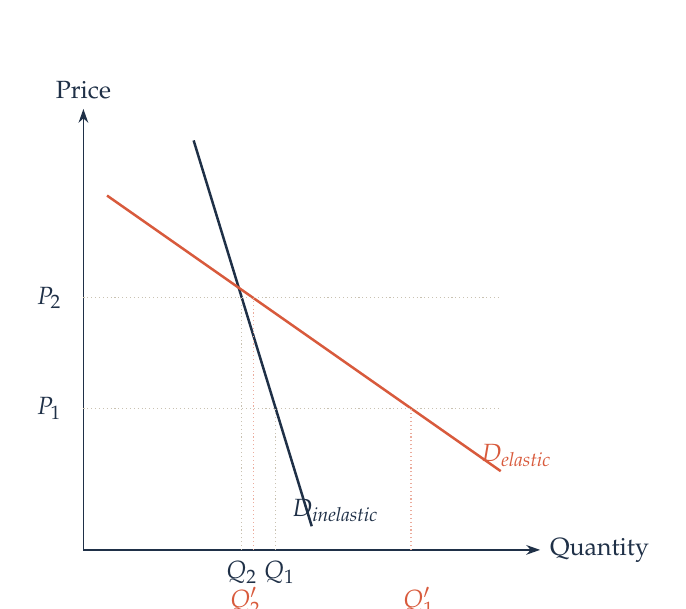
\begin{tikzpicture}[scale=1.0, baseline=(current bounding box.center)]
  % Axes
  \draw[econ axis] (0,0)--(5.8,0) node[axis label, right]{Quantity};
  \draw[econ axis] (0,0)--(0,5.6) node[axis label, above]{Price};

  % Relatively inelastic demand (steep)
  \draw[curve A] (1.4,5.2)--(2.9,0.3);
  \node[curve label, color=CurveNavy, font=\small\itshape] at (3.2,0.5) {$D_{\text{inelastic}}$};

  % Relatively elastic demand (shallow)
  \draw[curve B] (0.3,4.5)--(5.3,1.0);
  \node[curve label, color=CurveRose, font=\small\itshape] at (5.5,1.2) {$D_{\text{elastic}}$};

  % Common price levels
  \draw[guide line] (0,1.8)--(5.3,1.8);
  \draw[guide line] (0,3.2)--(5.3,3.2);
  \node[tick label, left] at (-0.15,1.8) {$P_1$};
  \node[tick label, left] at (-0.15,3.2) {$P_2$};

  % Quantity changes for inelastic curve
  % D_inelastic: (1.4,5.2)→(2.9,0.3), slope=−3.267, y=−3.267x+9.773
  % At P₁=1.8: x=2.44. At P₂=3.2: x=2.01.
  \draw[guide line] (2.44,0)--(2.44,1.8);
  \draw[guide line] (2.01,0)--(2.01,3.2);
  \node[tick label, below, font=\small] at (2.01,-0.02) {$Q_2$};
  \node[tick label, below, font=\small] at (2.49,-0.02) {$Q_1$};

  % Quantity changes for elastic curve
  % D_elastic: (0.3,4.5)--(5.3,1.0), slope=-0.7, y=-0.7x+4.71
  % At P₁=1.8: x=2.91/0.7=4.16. At P₂=3.2: x=1.51/0.7=2.16.
  \draw[guide line, color=CurveRose!50] (4.16,0)--(4.16,1.8);
  \draw[guide line, color=CurveRose!50] (2.16,0)--(2.16,3.2);
  \node[tick label, below, color=CurveRose, font=\small] at (2.06,-0.35) {$Q_2'$};
  \node[tick label, below, color=CurveRose, font=\small] at (4.26,-0.35) {$Q_1'$};
\end{tikzpicture}%
}{%
\textbf{\color{CurveNavy}Same price rise $P_1 \to P_2$:}\\[7pt]
\textbf{$D_{\text{inelastic}}$ (steep):} Quantity falls only slightly ($Q_1 \to Q_2$). Consumers have few alternatives.\\[6pt]
\textbf{\color{CurveRose}$D_{\text{elastic}}$ (shallow):} Quantity falls sharply ($Q_1' \to Q_2'$). Consumers can switch to substitutes.\\[8pt]
\textbf{\color{CurveGold}Key rule:}\enspace Steeper $=$ more inelastic. Flatter $=$ more elastic.%
}
\end{diagrambox}

\begin{diagrambox}[Figure V -- PED Varies Along a Straight-Line Demand Curve]
\diagramwithtext{%
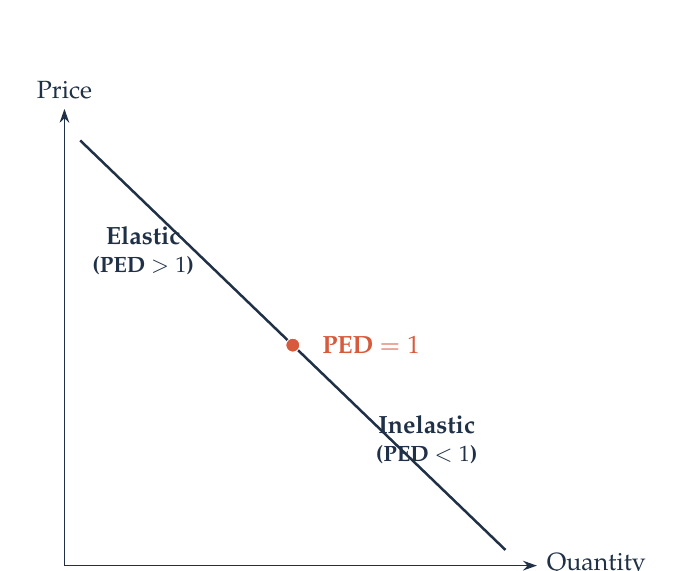
\begin{tikzpicture}[scale=1.0, baseline=(current bounding box.center)]
  % Axes
  \draw[econ axis] (0,0)--(6.0,0) node[axis label, right]{Quantity};
  \draw[econ axis] (0,0)--(0,5.8) node[axis label, above]{Price};

  % Demand curve
  \draw[curve A] (0.2,5.4)--(5.6,0.2);

  % Midpoint — clearly visible dot
  \node[econ point accent] at (2.9,2.8) {};
  \node[annot accent, font=\small\bfseries, anchor=west] at (3.15,2.8) {PED $= 1$};

  % Upper half: Elastic zone label — left of curve, clear space
  \node[axis label, font=\small\bfseries, color=CurveNavy, align=center]
    at (1.0,4.0) {Elastic\\[-1pt]{\footnotesize(PED $> 1$)}};

  % Lower half: Inelastic zone label — right of curve, clear space
  \node[axis label, font=\small\bfseries, color=CurveNavy, align=center]
    at (4.6,1.6) {Inelastic\\[-1pt]{\footnotesize(PED $< 1$)}};

  % Zone context is conveyed by the Elastic / Inelastic labels
  % and the accompanying text explanation — no axis annotations needed.
\end{tikzpicture}%
}{%
\textbf{\color{NavyPrimary}Reading the diagram:}\\[4pt]
At the \textbf{top} of the demand curve (high P, low Q), a 1\% price change causes a \textbf{larger percentage change} in quantity demanded $\Rightarrow$ demand is \textbf{elastic} (PED $> 1$).\\[6pt]
At the \textbf{bottom} of the demand curve (low P, high Q), the same 1\% price change causes a \textbf{smaller percentage change} in quantity demanded $\Rightarrow$ demand is \textbf{inelastic} (PED $< 1$).\\[6pt]
At the \textbf{midpoint}, PED $= 1$ (unit elastic). This is where total revenue is maximized.\\[8pt]
\textbf{\color{GoldAccent}Key:}\enspace Elasticity \emph{varies} along a straight-line demand curve. Do not confuse elasticity (responsiveness of \emph{percentage} changes) with slope (the angle of the curve).%
}
\end{diagrambox}

\subsubsection{Factors Affecting PED}

\begin{itemize}
  \item \textbf{Availability of substitutes:} More and closer substitutes $\Rightarrow$ more elastic (e.g.\ different cola brands).
  \item \textbf{Necessity vs.\ luxury:} Necessities are inelastic (insulin, salt); luxuries are elastic (sports cars).
  \item \textbf{Proportion of income:} Goods taking a large share of income are more elastic (cars vs.\ matches).
  \item \textbf{Time period:} Demand becomes more elastic over time as consumers find alternatives.
\end{itemize}

\subsubsection{PED and Total Expenditure}

\textbf{Total Expenditure} (TE) $=$ Price $\times$ Quantity. This is identical to \textbf{Total Revenue} (TR) earned by the firm -- what consumers spend is exactly what producers receive.

\begin{tcolorbox}[enhanced,colback=LightBlue,colframe=MidBlue!70,arc=0pt,boxrule=0.8pt]
\begin{tabular}{@{}>{\RaggedRight\arraybackslash}p{0.25\linewidth}>{\RaggedRight\arraybackslash}p{0.35\linewidth}>{\RaggedRight\arraybackslash}p{0.35\linewidth}@{}}
\textbf{\color{NavyPrimary}Elasticity} & \textbf{\color{NavyPrimary}Price Rises} & \textbf{\color{NavyPrimary}Price Falls} \\
\midrule
\textbf{Inelastic} (PED $< 1$) & TE \textbf{increases} & TE \textbf{decreases} \\
\textbf{Elastic} (PED $> 1$) & TE \textbf{decreases} & TE \textbf{increases} \\
\textbf{Unit Elastic} (PED $= 1$) & TE \textbf{unchanged} & TE \textbf{unchanged} \\
\end{tabular}
\end{tcolorbox}

\begin{coreidea}
\textbf{Why does TR rise when price rises and demand is inelastic?}

When demand is inelastic, a price rise causes only a \emph{small} fall in quantity demanded. Yes, fewer units are sold -- but each remaining customer pays a \emph{higher} price. The extra revenue gained per unit sold \textbf{more than offsets} the revenue lost from the small reduction in quantity. The net effect is a rise in total revenue.

Conversely, when demand is elastic, the quantity fall is so large that the revenue lost from lost customers \emph{outweighs} the gain from the higher price -- so TR falls.
\end{coreidea}

\begin{tcolorbox}[enhanced,colback=LightGold,colframe=GoldAccent,arc=0pt,boxrule=0.9pt,
  left=8pt,right=8pt,top=6pt,bottom=6pt]
\textbf{\color{NavyPrimary}Firm Strategy:} A firm can raise its price and \emph{increase} revenue if demand is inelastic. It should \emph{lower} its price to increase revenue if demand is elastic. Firms invest in branding and advertising to make demand more inelastic.
\end{tcolorbox}

\subsection{Income Elasticity of Demand (YED)}

\begin{keyterm}{Income Elasticity of Demand (YED)}
A measure of the \textbf{responsiveness of quantity demanded} to a change in consumer \textbf{income}.
\[
\text{YED} = \frac{\%\;\Delta\text{Quantity Demanded}}{\%\;\Delta\text{Income}}
\]
The \textbf{sign} of YED reveals whether the good is normal or inferior.
\end{keyterm}

\begin{example}[Calculating YED]
Average income rises from \$20{,}000 to \$22{,}000 (+10\%). Demand for restaurant meals rises from 50 to 60 per week (+20\%).
\[
\text{YED} = \frac{+20\%}{+10\%} = +2.0
\]
Positive and $> 1$: this is a \textbf{luxury good}.
\end{example}

\subsubsection{Interpreting YED: Sign and Size}

\begin{tcolorbox}[enhanced,colback=LightBlue,colframe=MidBlue!70,arc=0pt,boxrule=0.8pt]
\begin{tabular}{@{}>{\RaggedRight\arraybackslash}p{0.25\linewidth}>{\RaggedRight\arraybackslash}p{0.22\linewidth}>{\RaggedRight\arraybackslash}p{0.48\linewidth}@{}}
\textbf{\color{NavyPrimary}YED Value} & \textbf{\color{NavyPrimary}Type of Good} & \textbf{\color{NavyPrimary}Meaning} \\
\midrule
YED $> 1$ (positive) & Luxury / Superior & Demand rises more than proportionally with income. \\
$0 <$ YED $\leq 1$ & Normal necessity & Demand rises, but less than proportionally. \\
YED $< 0$ (negative) & Inferior Good & Demand \emph{falls} as income rises. \\
\end{tabular}
\end{tcolorbox}




\subsection{Cross Elasticity of Demand (XED)}



\begin{keyterm}{Cross Elasticity of Demand (XED)}
A measure of the \textbf{responsiveness of quantity demanded of Good A} to a change in the \textbf{price of Good B}.
\[
\text{XED} = \frac{\%\;\Delta\text{Quantity Demanded of Good A}}{\%\;\Delta\text{Price of Good B}}
\]
The \textbf{sign} reveals the relationship between the two goods.
\end{keyterm}

\begin{example}[Calculating XED]
The price of Coca-Cola rises by 20\%. Demand for Pepsi rises by 30\%.
\[
\text{XED}_{\text{Pepsi w.r.t.\ Coke}} = \frac{+30\%}{+20\%} = +1.5
\]
Positive XED: Coke and Pepsi are \textbf{substitutes}.
\end{example}

\begin{tcolorbox}[enhanced,colback=LightBlue,colframe=MidBlue!70,arc=0pt,boxrule=0.8pt]
\begin{tabular}{@{}>{\RaggedRight\arraybackslash}p{0.25\linewidth}>{\RaggedRight\arraybackslash}p{0.28\linewidth}>{\RaggedRight\arraybackslash}p{0.42\linewidth}@{}}
\textbf{\color{NavyPrimary}XED Sign} & \textbf{\color{NavyPrimary}Relationship} & \textbf{\color{NavyPrimary}Example} \\
\midrule
Positive ($+$) & \textbf{Substitutes} & Coke \& Pepsi; butter \& margarine \\
Negative ($-$) & \textbf{Complements} & Cars \& petrol; printers \& ink \\
Zero ($0$) & \textbf{Unrelated} & Tea \& concrete \\
\end{tabular}
\end{tcolorbox}

\begin{evaluation}{Elasticities of Demand (PED, YED, XED)}
\textbf{Strengths / Why Elasticity Is Critical:}
\begin{itemize}[leftmargin=*, nosep]
\item Enables precise prediction of real-world market outcomes — knowing demand elasticity tells you whether a tax will raise lots of revenue (inelastic demand) or drive consumers away (elastic demand).
\item Explains why firms set different prices in different markets: airline pricing varies based on time sensitivity (business travellers are inelastic, tourists are elastic).
\item Distinguishes between normal goods (YED positive) and inferior goods (YED negative), revealing how consumer preferences shift with income.
\end{itemize}

\textbf{Limitations:}
\begin{itemize}[leftmargin=*, nosep]
\item \textbf{Elasticity varies along the curve:} A straight-line demand curve has constant slope but changing elasticity. At high prices (small quantities), demand is inelastic; at low prices, it becomes elastic. This is sometimes glossed over in simple models.
\item \textbf{Time period matters:} Short-run elasticity and long-run elasticity differ. Elasticity is usually higher in the long run (consumers can adjust more fully). Ignoring this leads to flawed policy predictions.
\item \textbf{Substitutes and complements are not fixed:} Over time, new substitutes emerge. What was inelastic yesterday may be elastic today as technology expands alternatives (e.g., petrol cars face elastic demand now that EVs are viable).
\item \textbf{Cross-elasticity complexity:} Two goods may be substitutes in one context (tea and coffee) and complements in another (tea and biscuits). The concept simplifies a complex reality.
\end{itemize}

\textbf{It depends on\ldots}
\begin{itemize}[leftmargin=*, nosep]
\item \textbf{Availability of substitutes:} The more substitutes, the more elastic the demand. Cigarettes have few substitutes (other than quitting), so PED is low.
\item \textbf{Necessity vs. luxury:} Necessity goods (food, medicine) have inelastic demand; luxury goods (holidays, jewellery) have elastic demand. But this distinction blurs at the margin.
\item \textbf{Time horizon:} In the short run, people cannot easily switch (petrol cars cannot instantly become EVs). In the long run, they can. Long-run PED is typically higher than short-run PED.
\item \textbf{Income level:} For a poor household, a 10\% price rise in staple food is catastrophic (inelastic response). For a rich household, it is trivial. Elasticity depends on relative price burden.
\item \textbf{Share of budget:} Demand for a good that consumes 50\% of your budget is far more elastic than one consuming 0.1\%, because you have more incentive to economise.
\end{itemize}
\end{evaluation}

% ── Price Elasticity of Supply ───────────────────────────────
\section{Price Elasticity of Supply}



\subsection{Definition and Formula}

\begin{keyterm}{Price Elasticity of Supply (PES)}
A measure of the \textbf{responsiveness of quantity supplied} to a change in the good's own price.
\[
\text{PES} = \frac{\%\;\Delta\text{Quantity Supplied}}{\%\;\Delta\text{Price}}
\]
PES is \textbf{always positive} -- a higher price makes production more profitable, so firms supply more.
\end{keyterm}

\begin{example}[Calculating PES]
The price of strawberries rises from \$2.00 to \$2.50 per kg (+25\%). Farmers increase supply from 1{,}000 kg to 1{,}300 kg (+30\%).
\[
\text{PES} = \frac{+30\%}{+25\%} = +1.2
\]
PES $> 1$: supply is \textbf{elastic}.
\end{example}

\subsubsection{Interpreting PES Values}

\begin{tcolorbox}[enhanced,colback=LightBlue,colframe=MidBlue!70,arc=0pt,boxrule=0.8pt]
\begin{tabular}{@{}>{\RaggedRight\arraybackslash}p{0.28\linewidth}>{\RaggedRight\arraybackslash}p{0.18\linewidth}>{\RaggedRight\arraybackslash}p{0.46\linewidth}@{}}
\textbf{\color{NavyPrimary}Description} & \textbf{\color{NavyPrimary}Value} & \textbf{\color{NavyPrimary}Meaning} \\
\midrule
Perfectly Inelastic & PES $= 0$ & Quantity supplied cannot change at all. Vertical supply curve. \\
Inelastic & $0 <$ PES $< 1$ & Output increases by a smaller \% than the price rise. \\
Unit Elastic & PES $= 1$ & \%$\Delta Q_s =$ \%$\Delta P$ exactly. \\
Elastic & PES $> 1$ & Output increases by a larger \% than the price rise. \\
Perfectly Elastic & PES $= \infty$ & Firms supply any amount at one price. Horizontal supply curve. \\
\end{tabular}
\end{tcolorbox}

\begin{diagrambox}[Figure VI -- Price Elasticity of Supply: The Axis-Intercept Rule]

\textbf{\small\color{CurveNavy} Panel A: Which axis does the supply curve cross?}

\medskip
\diagramwithtext{%
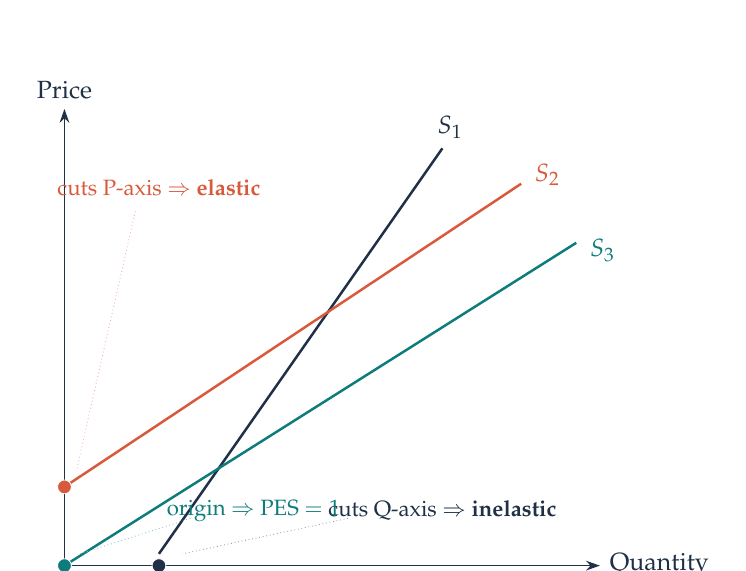
\begin{tikzpicture}[scale=1.0, baseline=(current bounding box.center)]
  % Axes - wide for clear separation
  \draw[econ axis] (0,0)--(6.8,0) node[axis label, right]{Quantity};
  \draw[econ axis] (0,0)--(0,5.8) node[axis label, above]{Price};

  % S1: Inelastic — cuts Q-axis (steepest curve)
  \draw[curve A] (1.2,0.15)--(4.8,5.3);
  \node[curve label, color=CurveNavy, anchor=south] at (4.9,5.3) {$S_1$};

  % S2: Elastic — cuts P-axis (medium slope)
  \draw[curve B] (0,1.0)--(5.8,4.85);
  \node[curve label, color=CurveRose, anchor=south west] at (5.85,4.7) {$S_2$};

  % S3: Unit elastic — through origin (shallowest)
  \draw[curve C] (0,0)--(6.5,4.1);
  \node[curve label, color=CurveSage, anchor=west] at (6.55,4.0) {$S_3$};

  % Mark intercepts with visible dots
  \node[econ point] at (1.2,0) {};
  \node[econ point accent] at (0,1.0) {};
  \node[econ point sage] at (0,0) {};

  % Annotations — placed in clear white space, well separated
  % S1 annotation: bottom-right area (below S3)
  \node[annot, color=CurveNavy, align=left] at (4.8,0.7)
    {cuts Q-axis $\Rightarrow$ \textbf{inelastic}};
  \draw[densely dotted, color=CurveNavy!50, line width=0.3pt]
    (3.6,0.6)--(1.5,0.15);

  % S2 annotation: top-left area (above all curves)
  \node[annot, color=CurveRose, align=left] at (1.2,4.8)
    {cuts P-axis $\Rightarrow$ \textbf{elastic}};
  \draw[densely dotted, color=CurveRose!50, line width=0.3pt]
    (0.9,4.5)--(0.15,1.2);

  % S3 annotation: bottom-centre area
  \node[annot, color=CurveSage, align=left] at (2.4,0.7)
    {origin $\Rightarrow$ PES $= 1$};
  \draw[densely dotted, color=CurveSage!50, line width=0.3pt]
    (1.6,0.6)--(0.2,0.15);
\end{tikzpicture}%
}{%
\textbf{\color{CurveNavy}The axis-intercept rule:}\\[6pt]
\textbf{$S_1$ crosses Q-axis:}\\[2pt]
PES $< 1$ (inelastic).\\[5pt]
\textbf{\color{CurveRose}$S_2$ crosses P-axis:}\\[2pt]
PES $> 1$ (elastic).\\[5pt]
\textbf{\color{CurveSage}$S_3$ through origin:}\\[2pt]
PES $= 1$ at every point.\\[8pt]
{\color{CurveRose}\textbf{Caution:}}\enspace The \emph{slope} does not determine elasticity.%
}
\end{diagrambox}

\begin{diagrambox}[Figure VIb -- Two Unit-Elastic Supply Curves Through the Origin]
\diagramwithtext{%
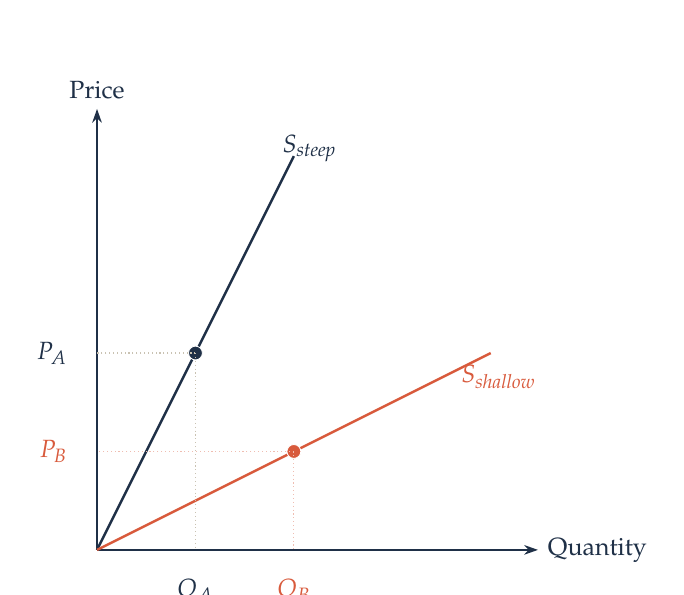
\begin{tikzpicture}[scale=1.0, baseline=(current bounding box.center)]
  % Axes
  \draw[econ axis] (0,0)--(5.6,0) node[axis label, right]{Quantity};
  \draw[econ axis] (0,0)--(0,5.6) node[axis label, above]{Price};

  % Steep curve through origin
  \draw[curve A] (0,0)--(2.5,5.0);
  \node[curve label, color=CurveNavy] at (2.7,5.1) {$S_{\text{steep}}$};

  % Shallow curve through origin
  \draw[curve B] (0,0)--(5.0,2.5);
  \node[curve label, color=CurveRose] at (5.1,2.2) {$S_{\text{shallow}}$};

  % Point on steep curve (higher price)
  \node[econ point] at (1.25,2.5) {};
  \draw[guide line] (1.25,2.5)--(1.25,0);
  \node[tick label, below] at (1.25,-0.25) {$Q_A$};
  \draw[guide line] (1.25,2.5)--(0,2.5);
  \node[tick label, left] at (-0.25,2.5) {$P_A$};

  % Point on shallow curve (lower price)
  \node[econ point accent] at (2.5,1.25) {};
  \draw[guide line, color=CurveRose!40] (2.5,1.25)--(2.5,0);
  \node[tick label, color=CurveRose, below] at (2.5,-0.25) {$Q_B$};
  \draw[guide line, color=CurveRose!40] (2.5,1.25)--(0,1.25);
  \node[tick label, color=CurveRose, left] at (-0.25,1.25) {$P_B$};
\end{tikzpicture}%
}{%
\textbf{\color{CurveNavy}A popular A Level trap:}\\[6pt]
Both curves pass through the origin. Despite \emph{very different slopes}, both have PES $= 1$ at every point.\\[6pt]
At any point: $\frac{P}{Q} = \frac{\Delta P}{\Delta Q}$, so:
\[
\text{PES} = \frac{\Delta Q}{\Delta P} \cdot \frac{P}{Q} = 1
\]
{\color{CurveRose}\textbf{Slope alone tells you nothing.}}\enspace What matters is where the curve intersects the axes.%
}
\end{diagrambox}

\subsection{Factors Affecting PES}

\subsubsection{Time Period -- The Most Important Factor}

\begin{tcolorbox}[enhanced,colback=LightBlue,colframe=MidBlue!70,arc=0pt,boxrule=0.8pt]
\begin{tabular}{@{}>{\RaggedRight\arraybackslash}p{0.25\linewidth}>{\RaggedRight\arraybackslash}p{0.7\linewidth}@{}}
\textbf{\color{NavyPrimary}Time Period} & \textbf{\color{NavyPrimary}Ability to Respond} \\
\midrule
\textbf{Momentary} & Supply is fixed at what is already produced. PES $= 0$. \\
\textbf{Short Run} & Firms can vary labour and hours but capital is fixed. Supply is \emph{inelastic} unless spare productive capacity already exists. If factories are running near full capacity, output cannot easily be expanded even with higher prices. \\
\textbf{Long Run} & Firms build new factories; new firms enter. Supply becomes highly elastic. \\
\end{tabular}
\end{tcolorbox}

Other factors include:
\begin{itemize}
  \item \textbf{Spare productive capacity:} Idle factories allow quick output increases $\Rightarrow$ elastic supply.
  \item \textbf{Availability of stocks:} Large inventories allow immediate release onto the market $\Rightarrow$ elastic supply. (Perishable goods cannot be stocked $\Rightarrow$ inelastic.)
  \item \textbf{Mobility of factors:} If resources can easily switch between uses, supply is more elastic.
  \item \textbf{Complexity of production:} Simple processes (printing T-shirts) are elastic; complex ones (building a cruise ship) are inelastic.
\end{itemize}

\subsubsection{Agricultural Markets: A Case Study in Inelastic Supply}

Agricultural markets are a classic example of \emph{inelastic supply} causing price volatility:
\begin{itemize}
  \item \textbf{Time lags:} Growing crops and raising livestock takes months or years.
  \item \textbf{Perishability:} Most farm produce cannot be stored long-term.
  \item \textbf{Dependence on nature:} Weather, pests, and disease are outside farmer control.
\end{itemize}

\textbf{Consequence:} A bumper harvest (large supply increase) combines with inelastic food demand to cause a \emph{sharp price fall} -- farmers' total revenue can collapse. A poor harvest causes a sharp price spike. This creates dangerous price volatility and income uncertainty for farmers.

\begin{evaluation}{Price Elasticity of Supply}
\textbf{Strengths / Practical Applications:}
\begin{itemize}[leftmargin=*, nosep]
\item Explains tax incidence: if supply is inelastic (agriculture, land), producers bear most of a tax burden; if demand is inelastic, consumers bear most.
\item Predicts market volatility: inelastic supply with elastic demand creates price spikes when demand rises (e.g., oil shocks). This helps governments design stabilisation policies.
\item Informs industrial policy: governments subsidise nascent industries because short-run PES is low. Without subsidy, a price squeeze forces exit; with subsidy, firms survive long enough to build capacity.
\end{itemize}

\textbf{Limitations:}
\begin{itemize}[leftmargin=*, nosep]
\item \textbf{Time periods are artificial:} The momentary, short-run, and long-run distinctions are somewhat arbitrary. Supply response is a continuous process, not a series of discrete jumps.
\item \textbf{Capital adjustment is non-linear:} Building a new factory is not a smooth process. A firm may sit idle until a threshold price justifies the fixed capital cost. Below that threshold, PES is zero; above it, PES jumps. This non-linearity is missed by the standard framework.
\item \textbf{Ignores expectations:} Farmers' planting decisions depend on expected future prices, not just current prices. If they expect prices to fall, they reduce supply even when current prices rise. The framework treats supply as a mechanical response to current prices.
\item \textbf{Assumes constant technology:} In reality, supply response often involves technological innovation, which itself depends on price signals and profitability. A purely mechanical elasticity misses this.
\end{itemize}

\textbf{It depends on\ldots}
\begin{itemize}[leftmargin=*, nosep]
\item \textbf{Time horizon:} Short-run PES is almost always lower than long-run PES. Supply becomes far more responsive once firms can build new plants, workers can retrain, and new entrants arrive.
\item \textbf{Industry characteristics:} Primary industries (agriculture, mining) have inelastic supply because of nature's constraints. Manufacturing can be more elastic. Services (consulting, hospitality) can be very elastic because they require few fixed assets.
\item \textbf{Spare capacity:} An industry running at 50\% capacity can respond to price increases very elastically; one at 95\% capacity is inelastic.
\item \textbf{Price expectations:} If farmers expect prices to fall next year, they will not expand supply even if prices rise now. Elasticity depends on whether the price rise is expected to be permanent or temporary.
\end{itemize}
\end{evaluation}

% ── The Interaction of Demand and Supply ─────────────────────
\section{The Interaction of Demand and Supply}



\subsection{Market Equilibrium and Disequilibrium}

\begin{keyterm}{Market Equilibrium}
The state where \textbf{quantity demanded equals quantity supplied} (Qd $=$ Qs) at the \textbf{equilibrium price}. There is no pressure for the price to change. On a diagram, equilibrium is at the \emph{intersection} of the demand and supply curves.
\end{keyterm}

\begin{keyterm}{Disequilibrium}
A state where Qd $\neq$ Qs. The price mechanism automatically corrects this:
\begin{itemize}
  \item \textbf{Excess Demand (Shortage):} Price is below equilibrium. Qd $>$ Qs. Consumers compete for the good, \emph{pushing prices up} towards equilibrium.
  \item \textbf{Excess Supply (Surplus):} Price is above equilibrium. Qs $>$ Qd. Firms cut prices to sell unsold stock, \emph{pushing prices down} towards equilibrium.
\end{itemize}
\end{keyterm}

\begin{diagrambox}[Figure VII -- Market Equilibrium, Shortage and Surplus]
\diagramwithtext{%
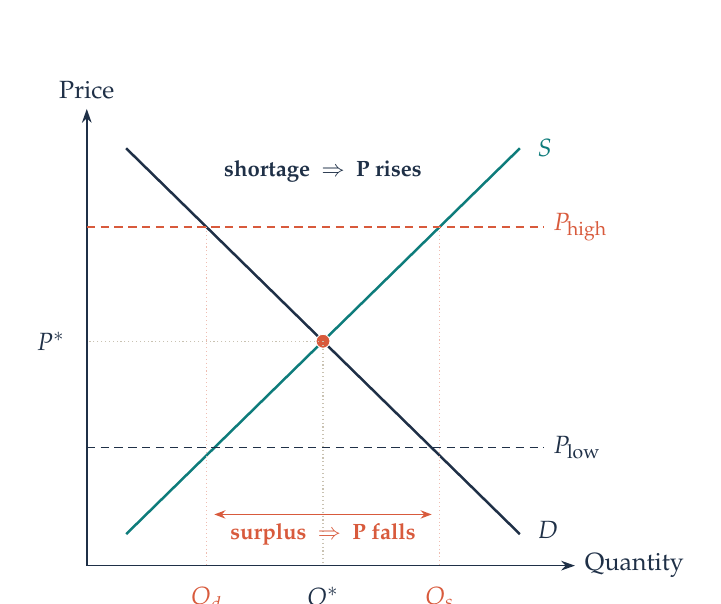
\begin{tikzpicture}[scale=1.0, baseline=(current bounding box.center)]
  % Axes
  \draw[econ axis] (0,0)--(6.2,0) node[axis label, right]{Quantity};
  \draw[econ axis] (0,0)--(0,5.8) node[axis label, above]{Price};

  % Demand curve
  \draw[curve A] (0.5,5.3)--(5.5,0.4);
  \node[curve label, color=CurveNavy, anchor=west] at (5.6,0.45) {$D$};

  % Supply curve
  \draw[curve C] (0.5,0.4)--(5.5,5.3);
  \node[curve label, color=CurveSage, anchor=west] at (5.6,5.3) {$S$};

  % Equilibrium
  \node[econ point accent] at (3.0,2.85) {};
  \draw[guide line] (3.0,2.85)--(3.0,0);
  \node[tick label, below] at (3.0,-0.15) {$Q^*$};
  \draw[guide line] (3.0,2.85)--(0,2.85);
  \node[tick label, left] at (-0.15,2.85) {$P^*$};

  % Price above equilibrium -- surplus
  % D at P=4.3: −0.98x+5.79=4.3 → x=1.52. S at P=4.3: 0.98x−0.09=4.3 → x=4.48
  \draw[line width=0.5pt, color=CurveRose, densely dashed] (0,4.3)--(5.8,4.3);
  \node[annot, color=CurveRose, right, font=\small] at (5.8,4.3) {$P_{\text{high}}$};
  \draw[guide line, color=CurveRose!40] (1.52,4.3)--(1.52,0);
  \node[tick label, color=CurveRose, below, font=\small] at (1.52,-0.15) {$Q_d$};
  \draw[guide line, color=CurveRose!40] (4.48,4.3)--(4.48,0);
  \node[tick label, color=CurveRose, below, font=\small] at (4.48,-0.15) {$Q_s$};
  \draw[{Stealth[length=4pt]}-{Stealth[length=4pt]}, color=CurveRose, line width=0.5pt] (1.62,0.65)--(4.38,0.65);
  \node[annot, color=CurveRose, font=\footnotesize\bfseries] at (3.0,0.4) {surplus\enspace$\Rightarrow$\enspace P falls};

  % Price below equilibrium -- shortage
  \draw[line width=0.5pt, color=CurveNavy, densely dashed] (0,1.5)--(5.8,1.5);
  \node[annot, color=CurveNavy, right, font=\small] at (5.8,1.5) {$P_{\text{low}}$};
  \node[annot, color=CurveNavy, font=\footnotesize\bfseries] at (3.0,5.0) {shortage\enspace$\Rightarrow$\enspace P rises};
\end{tikzpicture}%
}{%
\textbf{\color{NavyPrimary}Reading the diagram:}\\[4pt]
At \textbf{equilibrium (P*, Q*)}, quantity demanded equals quantity supplied ($Q_d = Q_s$). There is no pressure for price to change.\\[6pt]
\textbf{Above equilibrium ($P_{\text{high}}$):}\enspace Supply exceeds demand ($Q_s > Q_d$), creating a \textbf{surplus}.\\[2pt]
Firms cut prices to sell unsold stock, pushing price \emph{downward} toward $P^*$.\\[6pt]
\textbf{Below equilibrium ($P_{\text{low}}$):}\enspace Demand exceeds supply ($Q_d > Q_s$), creating a \textbf{shortage}.\\[2pt]
Consumers compete for limited supply, pushing price \emph{upward} toward $P^*$.\\[8pt]
\textbf{\color{GoldAccent}Key:}\enspace The price mechanism automatically eliminates shortages and surpluses.\\[2pt]
Markets self-correct toward equilibrium without government intervention.%
}
\end{diagrambox}

\subsection{Effects of Shifts in Demand and Supply}

\begin{tcolorbox}[enhanced,colback=LightBlue,colframe=MidBlue!70,arc=0pt,boxrule=0.8pt]
\begin{tabular}{@{}>{\RaggedRight\arraybackslash}p{0.35\linewidth}>{\RaggedRight\arraybackslash}p{0.3\linewidth}>{\RaggedRight\arraybackslash}p{0.3\linewidth}@{}}
\textbf{\color{NavyPrimary}Change in Market} & \textbf{\color{NavyPrimary}Equilibrium Price} & \textbf{\color{NavyPrimary}Equilibrium Quantity} \\
\midrule
Demand Increases (D $\rightarrow$) & \textbf{Rises} & \textbf{Rises} \\
Demand Decreases (D $\leftarrow$) & \textbf{Falls} & \textbf{Falls} \\
Supply Increases (S $\rightarrow$) & \textbf{Falls} & \textbf{Rises} \\
Supply Decreases (S $\leftarrow$) & \textbf{Rises} & \textbf{Falls} \\
\midrule
Both D and S Increase & \textbf{Ambiguous} & \textbf{Rises} \\
D Increases, S Decreases & \textbf{Rises} & \textbf{Ambiguous} \\
\end{tabular}
\end{tcolorbox}

When both curves shift simultaneously, one of the outcomes (price or quantity) is always \emph{determinate}, but the other is \emph{ambiguous} and depends on the relative size of the two shifts.

\subsection{Relationships Between Different Markets}

Markets do not exist in isolation -- they are interconnected in four key ways:

\begin{itemize}
  \item \textbf{Joint Demand (Complements):} Goods used together. Higher demand for one raises demand for the other (e.g.\ printers and ink, cars and petrol). XED is \emph{negative}.
  \item \textbf{Competitive Demand (Substitutes):} Goods used in place of each other. Higher demand for one reduces demand for the other (e.g.\ butter and margarine). XED is \emph{positive}.
  \item \textbf{Derived Demand:} Demand for a factor of production that arises from the demand for the final product. The demand for steel is \emph{derived} from the demand for cars. The demand for bricklayers is \emph{derived} from the demand for new houses.
  \item \textbf{Joint Supply:} Production of one good automatically produces another. Refining crude oil yields petrol, diesel, and kerosene simultaneously. A cattle farm produces both beef and leather hides.
\end{itemize}

\subsection{Functions of Price in Resource Allocation}

\begin{tcolorbox}[enhanced,colback=LightBlue,colframe=MidBlue!70,arc=0pt,boxrule=0.8pt,
  left=10pt,right=10pt,top=8pt,bottom=8pt]
\begin{tabular}{@{}>{\RaggedRight\arraybackslash}p{0.20\linewidth}>{\RaggedRight\arraybackslash}p{0.35\linewidth}>{\RaggedRight\arraybackslash}p{0.38\linewidth}@{}}
\textbf{\color{NavyPrimary}Function} & \textbf{\color{NavyPrimary}How it Works} & \textbf{\color{NavyPrimary}Example} \\
\midrule
\textbf{Rationing} & Rising prices limit consumption to those willing and able to pay the most, ensuring scarce goods are not wasted. & Copper imports are banned $\Rightarrow$ domestic copper price rises $\Rightarrow$ copper is rationed to its highest-value uses (e.g.\ electronics and infrastructure rather than decorative purposes). \\
\textbf{Signalling} & Price changes transmit information about scarcity and surplus to all market participants without any central authority. & Rising EV prices signal: ``build more factories; consumers want this.'' \\
\textbf{Incentivising} & The profit motive drives resources into high-price industries and out of low-price ones. & High profits in EVs attract new firms and investment into the sector. \\
\end{tabular}
\end{tcolorbox}

\begin{tcolorbox}[enhanced,colback=EvalBg,colframe=EvalFrame,arc=0pt,boxrule=1pt,title={\bfseries\color{EvalFrame}Evaluation: The Price Mechanism and Elasticities},fonttitle=\small]
\small\RaggedRight
\begin{itemize}[itemsep=2pt,topsep=2pt]
  \item \textbf{PED/PES determines tax incidence:} The more inelastic demand relative to supply, the greater the consumer's share of an indirect tax. If supply is perfectly elastic, consumers bear the entire burden. \textit{``It depends on relative elasticities.''}
  \item \textbf{Market signals are not always reliable:} Externalities, public goods and merit goods cause market failure -- the price mechanism allocates resources efficiently \textit{only when} social and private costs/benefits coincide.
  \item \textbf{Short run vs. long run:} Supply is typically more inelastic in the short run (fixed factors); adjustment takes time. A short-run price spike may resolve itself as firms expand capacity.
  \item \textbf{Derived demand complication:} Labour demand is \emph{derived} from the demand for the final good a firm produces. When wages rise, firms face higher costs and pass these on as higher prices. Whether employment then falls depends on how consumers respond to that price rise. If demand for the final good is \textbf{inelastic} (e.g.\ petrol, medicine), consumers barely reduce their purchases, so firms still need nearly as many workers -- employment holds up. If demand for the final good is \textbf{elastic} (e.g.\ luxury goods), consumers cut back sharply when prices rise, so firms reduce output and shed workers -- employment falls significantly.
  \item \textbf{Income distribution:} Relying entirely on the price mechanism ignores equity -- markets allocate to those with purchasing power, not those with greatest need.
\end{itemize}
\end{tcolorbox}

\section{Consumer and Producer Surplus}

\subsection{Consumer Surplus}

\begin{keyterm}{Consumer Surplus}
The difference between the \textbf{maximum price a consumer is willing to pay} for a good and the \textbf{price they actually pay} (the market price). It represents the ``bargain'' or extra benefit gained from the transaction.

On a diagram, consumer surplus is the area \textbf{below the demand curve and above the market price}.
\end{keyterm}

\begin{example}[Consumer Surplus]
You would have been willing to pay \$15 for a pizza, but the market price is \$10. Your consumer surplus is \$5.
\end{example}

\subsection{Producer Surplus}

\begin{keyterm}{Producer Surplus}
The difference between the \textbf{price a producer actually receives} and the \textbf{minimum price they would have accepted} (their cost of production). It represents the extra gain beyond what is needed to cover costs.

On a diagram, producer surplus is the area \textbf{above the supply curve and below the market price}.
\end{keyterm}

\begin{example}[Producer Surplus]
A farmer would accept \$5 per bag of potatoes to cover costs, but the market price is \$7. The farmer earns \$2 producer surplus per bag.
\end{example}

\begin{diagrambox}[Figure VIII -- Consumer and Producer Surplus at Equilibrium]
\diagramwithtext{%
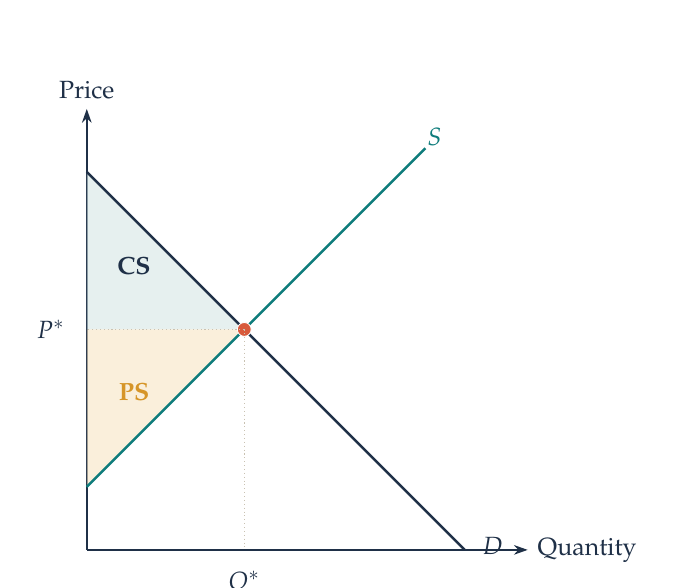
\begin{tikzpicture}[scale=1.0, baseline=(current bounding box.center)]
  % Axes
  \draw[econ axis] (0,0)--(5.6,0) node[axis label, right]{Quantity};
  \draw[econ axis] (0,0)--(0,5.6) node[axis label, above]{Price};

  % CS triangle (ice blue)
  \fill[FillPrimary, opacity=0.6] (0,4.8)--(2.0,2.8)--(0,2.8)--cycle;

  % PS triangle (sand wash)
  \fill[FillGold, opacity=0.6] (0,0.8)--(2.0,2.8)--(0,2.8)--cycle;

  % Demand curve
  \draw[curve A] (0.0,4.8)--(4.8,0.0);
  \node[curve label, color=CurveNavy, anchor=west] at (4.9,0.05) {$D$};

  % Supply curve
  \draw[curve C] (0.0,0.8)--(4.3,5.1);
  \node[curve label, color=CurveSage, anchor=south west] at (4.2,5.0) {$S$};

  % Equilibrium
  \node[econ point accent] at (2.0,2.8) {};
  \draw[guide line] (2.0,2.8)--(2.0,0);
  \node[tick label, below] at (2.0,-0.15) {$Q^*$};
  \draw[guide line] (2.0,2.8)--(0,2.8);
  \node[tick label, left] at (-0.15,2.8) {$P^*$};

  % Region labels
  \node[axis label, font=\small\bfseries, color=CurveNavy] at (0.6,3.6) {CS};
  \node[axis label, font=\small\bfseries, color=CurveGold] at (0.6,2.0) {PS};
\end{tikzpicture}%
}{%
\textbf{\color{CurveNavy}Consumer Surplus (CS):}\\[4pt]
Shaded area \emph{above} $P^*$ and \emph{below} $D$.\\
The total ``bargain'' enjoyed by all consumers.\\[8pt]
\textbf{\color{CurveGold}Producer Surplus (PS):}\\[4pt]
Shaded area \emph{below} $P^*$ and \emph{above} $S$.\\
The total gain above the minimum required to supply.\\[8pt]
\textbf{Total Surplus} $=$ CS $+$ PS represents total welfare gain from trade.%
}
\end{diagrambox}

\subsection{Causes of Changes in Consumer and Producer Surplus}

\begin{tcolorbox}[enhanced,colback=LightBlue,colframe=MidBlue!70,arc=0pt,boxrule=0.8pt]
\begin{tabular}{@{}>{\RaggedRight\arraybackslash}p{0.22\linewidth}>{\RaggedRight\arraybackslash}p{0.37\linewidth}>{\RaggedRight\arraybackslash}p{0.37\linewidth}@{}}
\textbf{\color{NavyPrimary}Price Change} & \textbf{\color{NavyPrimary}Consumer Surplus} & \textbf{\color{NavyPrimary}Producer Surplus} \\
\midrule
\textbf{Price Rises} & \textbf{Decreases.} Existing consumers pay more; some consumers are priced out of the market. & \textbf{Increases.} Producers receive higher revenue per unit and supply more. \\
\textbf{Price Falls} & \textbf{Increases.} Existing consumers pay less; new consumers enter the market. & \textbf{Decreases.} Producers receive less per unit and supply fewer units. \\
\end{tabular}
\end{tcolorbox}

\subsection{The Role of Elasticity in Determining the Extent of Changes}

The \emph{size} of a surplus change depends not only on the price change, but crucially on how responsive quantity is to that price change.

\subsubsection{PED and Consumer Surplus}

\begin{itemize}
  \item \textbf{Inelastic Demand (PED $<$ 1):} Consumers are ``locked in''; they continue buying a similar quantity even after a price change. Therefore, a price rise causes a \emph{large} loss of consumer surplus. A price fall causes a \emph{large} gain.
  \item \textbf{Elastic Demand (PED $>$ 1):} Consumers respond strongly, drastically cutting purchases on a price rise (or increasing on a price fall). The surplus change is spread over fewer units -- the change is \emph{smaller}.
\end{itemize}

\begin{example}[Petrol Tax (Inelastic)]
A government tax on petrol (inelastic demand) causes a large price rise but very little reduction in quantity. Consumers suffer a \emph{large loss} of consumer surplus because they must still buy nearly the same amount at the higher price.
\end{example}

\subsubsection{PES and Producer Surplus}

\begin{itemize}
  \item \textbf{Inelastic Supply (PES $<$ 1):} Producers cannot easily change output. A price rise therefore grants them a \emph{large} gain in producer surplus on nearly the same volume of sales. A price fall causes a \emph{large} loss.
  \item \textbf{Elastic Supply (PES $>$ 1):} Producers can expand output easily. New entrants compete away potential surpluses. The surplus change per unit is smaller.
\end{itemize}

\begin{example}[Vintage Wine (Inelastic Supply)]
A sudden surge in demand pushes up the price of vintage wine. Because supply is perfectly inelastic (no more of it can be produced), the entire price increase translates into an enormous gain in producer surplus for existing wine sellers.
\end{example}

\begin{evaluation}{Consumer and Producer Surplus}
\textbf{Strengths / Why Surplus Is Central to Microeconomic Policy:}
\begin{itemize}[leftmargin=*, nosep]
\item Quantifies the impact of price changes on buyer and seller welfare — enables government to measure the distributional consequences of taxes, price controls, and subsidies.
\item Shows that market equilibrium is Pareto efficient — at $P^*Q^*$, no one can be made better off without making someone worse off. Moving away from equilibrium (via controls or taxes) reduces total surplus.
\item Reveals tax incidence: the loss of consumer surplus to a tax partly goes to government revenue, and the rest is deadweight loss (wasted).
\end{itemize}

\textbf{Limitations:}
\begin{itemize}[leftmargin=*, nosep]
\item \textbf{Assumes linear demand/supply curves:} Most of the standard diagrams show triangular surplus regions, which is only accurate for linear curves. Real curves are often non-linear, making surplus areas curvilinear and harder to calculate.
\item \textbf{Ignores income distribution:} Total surplus says nothing about who gains and who loses. A policy that reduces total surplus but benefits the poor more than it harms the rich is often preferable to one that maximises total surplus at the cost of worsening inequality. Surplus analysis is silent on equity.
\item \textbf{Assumes preferences are stable:} Surplus calculation treats demand as fixed. But demand itself reflects preferences that may change with information, fashion, or social norms. The concept of "maximum" surplus becomes slippery if preferences are not exogenous.
\item \textbf{Difficult to measure in practice:} Calculating the area under the demand curve requires knowing the entire demand curve, which is rarely observable. Econometricians estimate it from limited data, introducing measurement error.
\item \textbf{Assumes willingness-to-pay reflects true welfare:} A consumer's willingness to pay reflects their ability to pay, not just their desire. A poor person may benefit enormously from a medicine but have zero willingness to pay. Surplus analysis overstates the importance of rich consumers' valuations.
\end{itemize}

\textbf{It depends on\ldots}
\begin{itemize}[leftmargin=*, nosep]
\item \textbf{Shape of demand and supply curves:} Linear curves give triangular surplus; curved lines give more complex shapes. The elasticity of the curves determines how surplus is divided between consumers and producers when prices change.
\item \textbf{Policy goal (equity vs. efficiency):} If maximising total welfare is the goal, policies should stay on the demand and supply curves. If distributing welfare to the poorest is the goal, violating market equilibrium may be justified despite DWL.
\item \textbf{Availability of other policy tools:} If the government can compensate losers from a surplus-reducing intervention (e.g., a tax), then the loss of total surplus is acceptable. Without compensation mechanisms, it is wasteful.
\item \textbf{Long-run vs. short-run:} Short-run surplus changes may be offset by long-run adjustments. A tax that reduces surplus temporarily may spur innovation that increases long-run surplus — the framework misses this dynamic.
\end{itemize}
\end{evaluation}

\section{Exam Practice Questions -- Chapter 2}

\begin{exampractice}
\begin{enumerate}[leftmargin=*]

\item \textbf{``Analyse the factors that determine the price elasticity of demand for a good, and explain why firms' revenue strategies depend on understanding elasticity.''} [15 marks]

\textit{Model structure: Define PED with formula $\to$ Identify determinants (substitutes availability, necessity vs. luxury, budget share, time horizon) $\to$ Draw diagrams showing elastic vs. inelastic demand curves $\to$ Analyse: if PED > 1, a price cut increases total revenue; if PED < 1, a price rise increases revenue $\to$ Real examples (cigarette tax yields revenue because inelastic; luxury goods cannot raise price much without losing sales) $\to$ Acknowledge that elasticity varies along a curve and over time.}

\item \textbf{``Using supply and demand diagrams, explain how a simultaneous increase in income and decrease in production costs would affect market equilibrium for a normal good.''} [15 marks]

\textit{Model structure: Set up initial S and D curves at equilibrium $\to$ Show D shifts right due to rising income (normal good) $\to$ Show S shifts right due to falling costs $\to$ Determine that Q$^*$ rises unambiguously but P$^*$ is ambiguous and depends on relative magnitudes of the two shifts $\to$ Draw alternative scenarios (small demand shift: price falls) vs. (large demand shift: price rises) $\to$ Use real examples (smartphones: both curves shifted right; manufacturing: supply gains exceeded demand gains so prices fell).}

\item \textbf{``Evaluate the use of taxation and subsidies as tools to correct the over- or under-consumption of demerit and merit goods respectively.''} [15 marks]

\textit{Model structure: Define merit/demerit goods and explain the information failure $\to$ Draw supply-demand diagrams showing socially optimal vs. market outcome $\to$ Show how a tax shifts demand left (for demerit goods) or a subsidy shifts supply right (for merit goods) $\to$ Discuss incidence: who bears the burden of the tax? Depends on relative elasticities $\to$ Evaluate limitations: taxes assume government knows the true cost; subsidies may be regressive (benefit wealthy as much as poor); behavioural responses may be smaller than predicted if demand is driven by addiction or preference, not just information $\to$ Conclude: taxes and subsidies work well if elasticity is moderate; they fail if demand is perfectly inelastic (tax doesn't reduce consumption) or perfectly elastic (subsidy is not needed).}

\item \textbf{``To what extent can consumer and producer surplus explain why government should not intervene in competitive markets?''} [15 marks]

\textit{Model structure: Define consumer surplus and producer surplus; show they are maximised at competitive equilibrium $\to$ Prove: at any other price/quantity combination, total surplus is smaller (deadweight loss exists) $\to$ Show examples: price ceiling creates DWL by reducing quantity below equilibrium; tax shifts equilibrium and reduces total surplus $\to$ Counter-arguments: (1) total surplus ignores distribution — a policy reducing total surplus but benefiting the poor is often preferable; (2) market failures mean competitive equilibrium is not socially optimal to begin with (externalities, public goods, information failure); (3) surplus analysis assumes static demand/supply but intervention might shift them (taxes fund R\&D, subsidies incentivise production) $\to$ Conclude: surplus analysis proves competitive markets are efficient in allocation, but efficiency is only one of several economic goals.}

\item \textbf{``Compare the relative effectiveness of using supply-side policies versus demand-side policies to achieve economic growth without causing inflation.''} [15 marks]

\textit{Model structure: Explain demand-side stimulus (fiscal/monetary expansion) shifts demand curve right $\to$ In a slack economy, this raises output without much price rise; in a tight economy, it causes demand-pull inflation $\to$ Explain supply-side policies (education, R\&D subsidies, deregulation) shift supply curve right $\to$ This raises output \emph{and} reduces prices — the best outcome $\to$ Discuss why supply-side is slower (takes years for education to impact labour supply) but more sustainable, while demand-side is faster but risks overheating $\to$ Use real contexts (post-2008: QE was demand-side, now facing inflation; 1980s: Reagan/Thatcher pursued supply-side reforms; Nordic countries balance both) $\to$ Conclude: for non-inflationary growth, supply-side is preferable, but requires long-term commitment.}

\end{enumerate}
\end{exampractice}

% ============================================================
%  CHAPTER 3: GOVERNMENT MICROECONOMIC INTERVENTION
% ============================================================
\chapter{Government Microeconomic Intervention}

\section{Reasons for Government Intervention in Markets}

\subsection{Addressing the Non-Provision of Public Goods}

\begin{coreidea}
Public goods have two defining characteristics that cause the free market to fail entirely: \textbf{non-excludability} and \textbf{non-rivalry}. Because no private firm can charge for them, they will not be provided without government action.
\end{coreidea}

\begin{keyterm}{Non-Excludability}
It is impossible (or prohibitively costly) to prevent someone who has not paid from consuming the good. You cannot stop a non-taxpayer from walking under a streetlamp.
\end{keyterm}

\begin{keyterm}{Non-Rivalry}
One person's consumption does not reduce the amount available for others. Your enjoyment of a lighthouse beam does not dim it for a passing ship.
\end{keyterm}

\subsubsection{Why the Free Market Fails to Provide Public Goods}

A private firm attempting to sell national defence or street lighting faces an insurmountable problem:
\begin{itemize}
  \item It \emph{cannot charge} for use because non-payers cannot be excluded.
  \item Every rational consumer therefore becomes a \textbf{free rider} -- enjoying the benefit without paying.
  \item Because no revenue can be generated, the firm has no incentive to produce the good at all.
  \item \textbf{Result:} Without intervention, public goods would be entirely absent from the economy despite society urgently needing them.
\end{itemize}

\subsubsection{Why Governments Provide Public Goods}

\begin{itemize}
  \item \textbf{Social welfare:} Goods like national defence, street lighting, public parks, and law enforcement are fundamental to safety, health, and economic activity.
  \item \textbf{Financing:} Since they cannot be sold, the government funds them through \emph{compulsory taxation}, which overcomes the free-rider problem by making payment unavoidable.
\end{itemize}

\subsection{Demerit Goods and Merit Goods}

\subsubsection{Demerit Goods -- Overconsumption}

\begin{keyterm}{Demerit Good (revisited)}
A good whose \textbf{true social cost exceeds its private cost}. The free market price is too low because it excludes the negative externalities imposed on third parties, so the good is \emph{overconsumed}.
\end{keyterm}

Why overconsumed in a free market:
\begin{itemize}
  \item \textbf{Information failure:} Consumers underestimate long-term personal harm (e.g.\ the true cancer risk of smoking).
  \item \textbf{Ignored social costs:} The market price only reflects private production costs -- it excludes the burden on public healthcare, lost productivity, and policing costs. Because social costs are omitted, the good is artificially cheap.
\end{itemize}

Government responses include indirect taxes (raising price to reflect true social cost), advertising bans, age restrictions, and public information campaigns.

\subsubsection{Merit Goods -- Underconsumption}

\begin{keyterm}{Merit Good (revisited)}
A good whose \textbf{true social benefit exceeds its private benefit}. The free market price is too high and quantity too low because consumers ignore the positive externalities their consumption generates for society.
\end{keyterm}

Why underconsumed in a free market:
\begin{itemize}
  \item \textbf{Information failure:} A young person may not appreciate the lifetime earnings boost of a good education.
  \item \textbf{Ignored social benefits:} A more educated, healthier, and vaccinated population benefits everyone -- but individuals only weigh their own private gain.
\end{itemize}

Government responses include free provision at the point of use, subsidies to lower the price, and legislation (e.g.\ compulsory schooling, mandatory vaccinations).

\subsection{Controlling Prices in Markets}

Governments sometimes conclude that the free market equilibrium price is too high (harming consumers) or too low (harming producers) and intervene directly with price controls.

\begin{tcolorbox}[enhanced,colback=LightBlue,colframe=MidBlue!70,arc=0pt,boxrule=0.8pt]
\begin{tabular}{@{}>{\RaggedRight\arraybackslash}p{0.20\linewidth}>{\RaggedRight\arraybackslash}p{0.38\linewidth}>{\RaggedRight\arraybackslash}p{0.38\linewidth}@{}}
& \textbf{\color{NavyPrimary}Maximum Price (Ceiling)} & \textbf{\color{NavyPrimary}Minimum Price (Floor)} \\
\midrule
\textbf{Set} & \emph{Below} equilibrium & \emph{Above} equilibrium \\
\textbf{Aim} & Protect consumers; make essentials affordable & Protect producers; guarantee minimum income \\
\textbf{Result} & \textbf{Shortage} (Qd $>$ Qs) & \textbf{Surplus} (Qs $>$ Qd) \\
\textbf{Examples} & Rent controls, food price caps, energy caps & National minimum wage, agricultural price supports \\
\end{tabular}
\end{tcolorbox}

\section{Methods and Effects of Government Intervention}

\subsection{Specific Indirect Taxes}

\begin{keyterm}{Specific Indirect Tax}
A \textbf{fixed monetary amount} of tax per unit sold (e.g.\ \pounds2 per bottle of wine), paid to the government by the seller. It \emph{shifts the supply curve vertically upward} by the exact amount of the tax.
\end{keyterm}

\subsubsection{Effects on the Market}

\begin{itemize}
  \item \textbf{Price rises} from P\textsubscript{1} to P\textsubscript{2} (but by less than the full tax).
  \item \textbf{Quantity falls} from Q\textsubscript{1} to Q\textsubscript{2}.
  \item \textbf{Government revenue} $=$ tax per unit $\times$ Q\textsubscript{2}.
\end{itemize}

\begin{diagrambox}[Figure IX -- Effect of a Specific Indirect Tax]
\diagramwithtext{%
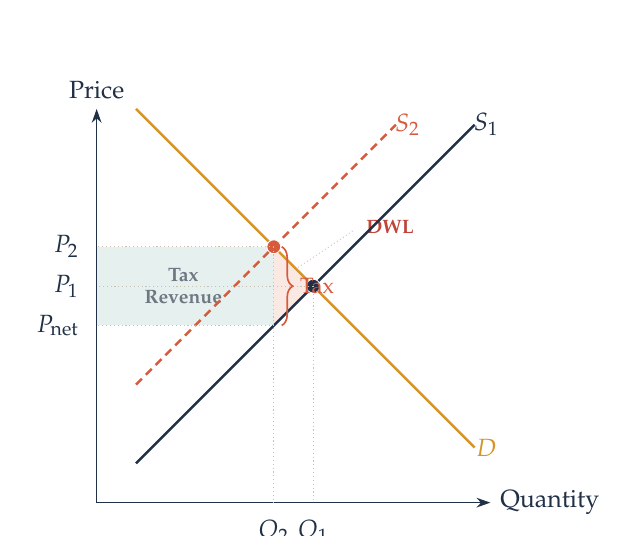
\begin{tikzpicture}[scale=1.0, baseline=(current bounding box.center)]
  % Econ axis
  \draw[econ axis] (0,0)--(5.0,0) node[axis label, right]{Quantity};
  \draw[econ axis] (0,0)--(0,5.0) node[axis label, above]{Price};

  % Tax revenue rectangle (from Q_2 at P_net to Q_2 at P_consumer)
  \fill[FillPrimary,opacity=0.6] (0,2.25) rectangle (2.25,3.25);
  \node[region label, color=AnnotGray, align=center, font=\scriptsize\bfseries] at (1.1,2.75) {Tax\\Revenue};

  % DWL triangle (from Q_2 to Q_1, bounded by D and S1)
  \fill[FillNegative,opacity=0.5] (2.25,3.25) -- (2.75,2.75) -- (2.25,2.25) -- cycle;
  % DWL label — outside the small triangle, with leader line
  \node[region label, color=CurveDanger, anchor=west] at (3.3,3.5) {DWL};
  \draw[densely dotted, color=CurveDanger!50, line width=0.3pt] (3.25,3.45)--(2.5,2.95);

  % Original supply: P = Q (trimmed to axis bounds)
  \draw[curve A] (0.5,0.5)--(4.8,4.8);
  \node[curve label, color=CurveNavy] at (4.95,4.8) {$S_1$};

  % Tax-shifted supply: P = Q + 1.0 (trimmed so top stays within axes)
  \draw[curve B shift] (0.5,1.5)--(3.8,4.8);
  \node[curve label, color=CurveRose] at (3.95,4.8) {$S_2$};

  % Demand curve: P = 5.5 - Q (trimmed to axis bounds)
  \draw[curve D] (0.5,5.0)--(4.8,0.7);
  \node[curve label, color=CurveGold] at (4.95,0.7) {$D$};

  % Original equilibrium E1: Q=2.75, P=2.75
  \node[econ point] at (2.75,2.75) {};
  \draw[guide line] (2.75,2.75)--(2.75,0);
  \node[tick label, below] at (2.75,-0.1) {$Q_1$};
  \draw[guide line] (2.75,2.75)--(0,2.75);
  \node[tick label, left] at (-0.1,2.75) {$P_1$};

  % New equilibrium E2: Q=2.25, P=3.25
  \node[econ point accent] at (2.25,3.25) {};
  \draw[guide line] (2.25,3.25)--(2.25,0);
  \node[tick label, below] at (2.25,-0.1) {$Q_2$};
  \draw[guide line] (2.25,3.25)--(0,3.25);
  \node[tick label, left] at (-0.1,3.25) {$P_2$};

  % Producer net price (on S1 at Q_2): P = Q_2 = 2.25
  \draw[guide line] (2.25,2.25)--(0,2.25);
  \node[tick label, left] at (-0.1,2.25) {$P_{\text{net}}$};

  % Tax per unit brace
  \draw[decorate,decoration={brace,amplitude=4pt,mirror},color=CurveRose, line width=0.6pt]
        (2.35,2.25)--(2.35,3.25) node[midway,right,xshift=3pt,annot,color=CurveRose]{Tax};
\end{tikzpicture}%
}{%
\textbf{\color{CurveNavy}Reading the diagram:}\\[4pt]
\textbf{$P_2$:} Price paid by consumers (rises)\\[2pt]
\textbf{$P_{\text{net}}$:} Price received by producers (falls)\\[2pt]
\textbf{Shaded area:} Government revenue $=$ tax $\times Q_2$\\[6pt]
\textbf{\color{CurveRose}Consumer burden:} $P_2 - P_1$\\[2pt]
\textbf{\color{CurveRose}Producer burden:} $P_1 - P_{\text{net}}$\\[2pt]
Together = full tax per unit.%
}
\end{diagrambox}

\subsubsection{Tax Incidence: Who Bears the Burden?}

\textbf{Tax incidence} refers to how the tax burden is divided between consumers and producers. It is determined by the relative elasticities of demand and supply.

\begin{tcolorbox}[enhanced,colback=LightBlue,colframe=MidBlue!70,arc=0pt,boxrule=0.8pt]
\begin{tabular}{@{}>{\RaggedRight\arraybackslash}p{0.38\linewidth}>{\RaggedRight\arraybackslash}p{0.58\linewidth}@{}}
\textbf{\color{NavyPrimary}Elasticity Condition} & \textbf{\color{NavyPrimary}Who Bears More of the Tax?} \\
\midrule
Demand \textbf{inelastic} (PED $<$ 1) & \textbf{Consumers} bear more. Firms pass the tax on; consumers still buy despite the higher price. (e.g.\ cigarettes, petrol.) \\
Demand \textbf{elastic} (PED $>$ 1) & \textbf{Producers} bear more. Raising prices causes a large drop in sales, so firms must absorb most of the tax. \\
Supply \textbf{inelastic} (PES $<$ 1) & \textbf{Producers} bear more. They cannot easily reduce output. \\
Supply \textbf{elastic} (PES $>$ 1) & \textbf{Consumers} bear more. Firms can easily redirect production. \\
\end{tabular}
\end{tcolorbox}

\subsection{Subsidies}

\begin{keyterm}{Subsidy}
A \textbf{per-unit payment from the government to producers}, designed to lower costs and encourage production and consumption. It \emph{shifts the supply curve vertically downward} by the amount of the subsidy.
\end{keyterm}

\subsubsection{Reasons for Subsidies}

\begin{itemize}
  \item Encourage consumption of merit goods (education, healthcare, public transport).
  \item Support low-income households (subsidised food, housing).
  \item Protect strategic domestic industries (e.g.\ renewable energy).
  \item Shield domestic producers from foreign competition.
\end{itemize}

\subsubsection{Effects on the Market}

\begin{itemize}
  \item \textbf{Price falls} from P\textsubscript{1} to P\textsubscript{2} (consumer pays less).
  \item \textbf{Quantity rises} from Q\textsubscript{1} to Q\textsubscript{2}.
  \item \textbf{Government cost} $=$ subsidy per unit $\times$ Q\textsubscript{2}.
  \item \textbf{Producer benefit:} receives P\textsubscript{2} from buyer \emph{plus} the subsidy, giving a net price above the original P\textsubscript{1}.
\end{itemize}

\begin{tcolorbox}[enhanced,colback=LightGold,colframe=GoldAccent,arc=0pt,boxrule=0.9pt,
  left=8pt,right=8pt,top=6pt,bottom=6pt]
\textbf{\color{NavyPrimary}Mirror image of a tax:} A subsidy shifts the supply curve \emph{downward}, a tax shifts it \emph{upward}. The incidence logic is identical -- elastic demand means consumers capture more of the benefit; inelastic demand means producers capture more.
\end{tcolorbox}


\begin{diagrambox}[Effect of a Subsidy on Market Price and Quantity]
\diagramwithtext{%
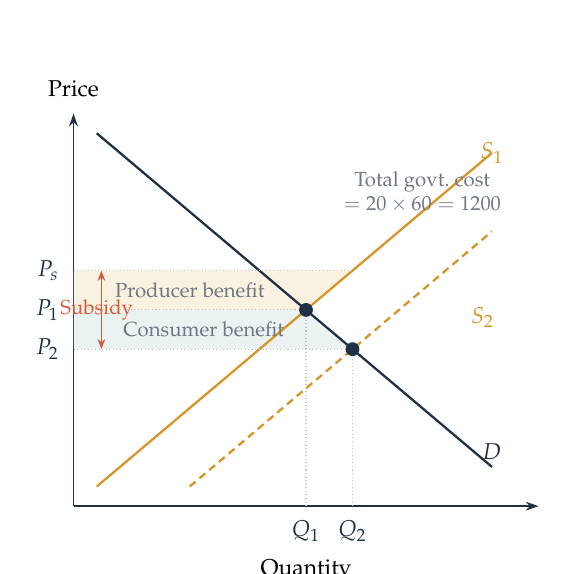
\begin{tikzpicture}[scale=0.92]
  \begin{axis}[
    econ chart,
    xlabel style={at={(ticklabel cs:0.5)}, anchor=north},
    width=8.0cm, height=7.0cm,
    xmax=100, ymax=100,
    xlabel={\small Quantity},
    ylabel={\small Price},
    xtick={50, 60}, xticklabels={$Q_1$, $Q_2$},
    ytick={40, 50, 60}, yticklabels={$P_2$, $P_1$, $P_s$},
  ]
    % Consumer benefit shading: trapezoid from (50,50) to (60,40) and back
    \fill[FillPrimary, opacity=0.5]
      (axis cs:0,50) -- (axis cs:50,50) -- (axis cs:60,40) -- (axis cs:0,40) -- cycle;
    % Producer benefit shading: trapezoid from (50,50) to (60,60) and back
    \fill[FillGold, opacity=0.5]
      (axis cs:0,50) -- (axis cs:50,50) -- (axis cs:60,60) -- (axis cs:0,60) -- cycle;
    % Demand curve: P = -Q + 100
    \addplot[curve primary, domain=5:90] {-x + 100};
    \node[curve label, color=CurveNavy] at (axis cs:90,14) {$D$};
    % Original supply: P = Q
    \addplot[curve accent, domain=5:90] {x};
    \node[curve label, color=CurveGold] at (axis cs:90,90) {$S_1$};
    % New supply after subsidy: P = Q - 20
    \addplot[curve accent shift, domain=25:90] {x - 20};
    \node[curve label, color=CurveGold] at (axis cs:88,48) {$S_2$};
    % Guide projections
    \addplot[guide projection] coordinates {(50,0)(50,50)(0,50)};
    \addplot[guide projection] coordinates {(60,0)(60,40)(0,40)};
    \addplot[guide projection] coordinates {(60,60)(0,60)};
    % Equilibrium points: E1 at (50,50), E2 at (60,40)
    \addplot[econ point] coordinates {(50,50)(60,40)};
    % Subsidy arrow from consumer price (40) to producer price (60)
    \draw[{Stealth[length=4pt]}-{Stealth[length=4pt]}, line width=0.6pt, color=CurveRose]
      (axis cs:6,40) -- (axis cs:6,60);
    \node[annot, color=CurveRose] at (axis cs:5,50) {Subsidy};
    % Region labels
    \node[annot, color=AnnotGray] at (axis cs:28,45) {Consumer benefit};
    \node[annot, color=AnnotGray] at (axis cs:25,55) {Producer benefit};
    \node[annot, color=AnnotGray, align=center] at (axis cs:75,80)
      {Total govt.\ cost\\$= 20 \times 60 = 1200$};
  \end{axis}
\end{tikzpicture}%
}{%
\textbf{\color{NavyPrimary}Subsidy Effect}\\[4pt]
$\bullet$ Supply shifts right from S\textsubscript{1} to S\textsubscript{2}\\[2pt]
$\bullet$ Consumer price falls from P\textsubscript{1} to P\textsubscript{2}; producer receives P\textsubscript{s}\\[2pt]
$\bullet$ Quantity rises from Q\textsubscript{1} to Q\textsubscript{2}\\[2pt]
$\bullet$ Blue area = consumer benefit; gold area = producer benefit\\[2pt]
$\bullet$ Total government cost = subsidy per unit \(\times\) Q\textsubscript{2}\\[2pt]
\textbf{\color{GoldAccent}Key:} Subsidy splits benefit between consumer and producer depending on PED/PES%
}
\end{diagrambox}

\subsection{Direct Provision of Goods and Services}

The government provides certain goods and services \emph{free at the point of use} (funded through taxation):

\begin{itemize}
  \item \textbf{Public goods:} National defence, street lighting -- the free market provides zero due to the free-rider problem.
  \item \textbf{Merit goods:} State education, public healthcare, libraries -- to correct underconsumption and ensure equitable access regardless of income.
  \item \textbf{Equity argument:} All citizens should have access to essential services irrespective of their ability to pay.
\end{itemize}

\subsection{Maximum and Minimum Prices}

\begin{diagrambox}[Figure X -- Maximum Price (Shortage) and Minimum Price (Surplus)]
\twodiagrams{%
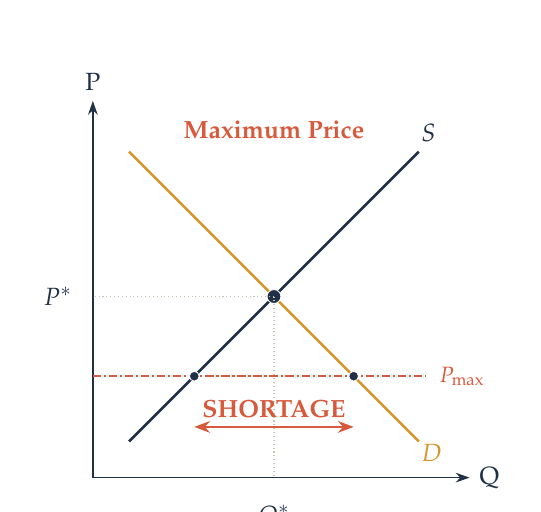
\begin{tikzpicture}[scale=0.92, baseline=(current bounding box.center)]
  \begin{scope}
  \clip (-0.9,-0.7) rectangle (5.8,5.6);
  \draw[econ axis] (0,0)--(5.2,0) node[axis label, right]{Q};
  \draw[econ axis] (0,0)--(0,5.2) node[axis label, above]{P};
  % Supply curve
  \draw[curve A] (0.5,0.5)--(4.5,4.5);
  \node[curve label, color=CurveNavy, anchor=south west] at (4.4,4.5) {$S$};
  % Demand curve
  \draw[curve D] (0.5,4.5)--(4.5,0.5);
  \node[curve label, color=CurveGold, anchor=north west] at (4.4,0.6) {$D$};
  % Equilibrium point
  \node[econ point] at (2.5,2.5) {};
  \draw[guide line] (2.5,2.5)--(0,2.5);
  \draw[guide line] (2.5,2.5)--(2.5,0);
  \node[tick label, left] at (-0.15,2.5) {$P^*$};
  \node[tick label, below] at (2.5,-0.25) {$Q^*$};
  % Maximum price line (below equilibrium)
  \draw[price floor, color=CurveRose] (0,1.4)--(4.6,1.4);
  \node[annot, color=CurveRose, anchor=west] at (4.65,1.4) {$P_{\max}$};
  % Shortage: Qd > Qs at Pmax
  \node[econ point, minimum size=3.5pt] at (1.4,1.4) {};
  \node[econ point, minimum size=3.5pt] at (3.6,1.4) {};
  \draw[{Stealth}-{Stealth}, color=CurveRose, line width=0.6pt] (1.4,0.7)--(3.6,0.7);
  \node[annot, color=CurveRose, font=\small\bfseries] at (2.5,0.95) {SHORTAGE};
  % Title
  \node[annot, color=CurveRose, font=\small\bfseries] at (2.5,4.8) {Maximum Price};
  \end{scope}
\end{tikzpicture}%
}{%
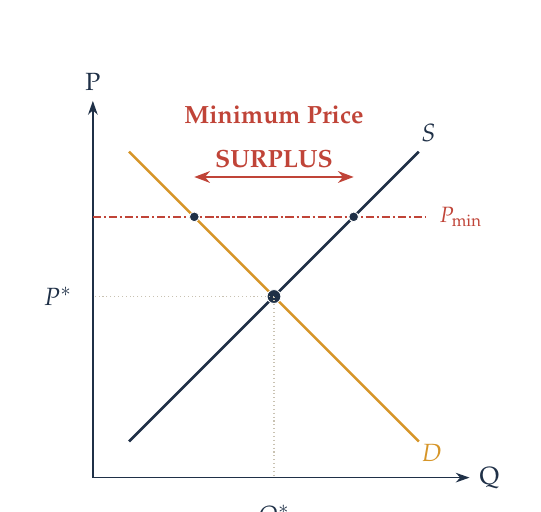
\begin{tikzpicture}[scale=0.92, baseline=(current bounding box.center)]
  \begin{scope}
  \clip (-0.9,-0.7) rectangle (5.8,5.6);
  \draw[econ axis] (0,0)--(5.2,0) node[axis label, right]{Q};
  \draw[econ axis] (0,0)--(0,5.2) node[axis label, above]{P};
  % Supply curve
  \draw[curve A] (0.5,0.5)--(4.5,4.5);
  \node[curve label, color=CurveNavy, anchor=south west] at (4.4,4.5) {$S$};
  % Demand curve
  \draw[curve D] (0.5,4.5)--(4.5,0.5);
  \node[curve label, color=CurveGold, anchor=north west] at (4.4,0.6) {$D$};
  % Equilibrium point
  \node[econ point] at (2.5,2.5) {};
  \draw[guide line] (2.5,2.5)--(0,2.5);
  \draw[guide line] (2.5,2.5)--(2.5,0);
  \node[tick label, left] at (-0.15,2.5) {$P^*$};
  \node[tick label, below] at (2.5,-0.25) {$Q^*$};
  % Minimum price line (above equilibrium)
  \draw[price floor] (0,3.6)--(4.6,3.6);
  \node[annot, color=CurveDanger, anchor=west] at (4.65,3.6) {$P_{\min}$};
  % Surplus: Qs > Qd at Pmin
  \node[econ point, minimum size=3.5pt] at (1.4,3.6) {};
  \node[econ point, minimum size=3.5pt] at (3.6,3.6) {};
  \draw[{Stealth}-{Stealth}, color=CurveDanger, line width=0.6pt] (1.4,4.15)--(3.6,4.15);
  \node[annot, color=CurveDanger, font=\small\bfseries] at (2.5,4.4) {SURPLUS};
  % Title
  \node[annot, color=CurveDanger, font=\small\bfseries] at (2.5,5.0) {Minimum Price};
  \end{scope}
\end{tikzpicture}%
}
\end{diagrambox}

\subsubsection{Maximum Price -- Consequences}

\begin{itemize}
  \item \textbf{Shortage:} Qd $>$ Qs at the controlled price.
  \item \textbf{Black markets:} Some consumers willing to pay above the legal maximum trade illegally.
  \item \textbf{Non-price rationing:} Queuing, waiting lists, or government allocation replace the price mechanism.
  \item \textbf{Reduced quality:} Suppliers face lower revenue and have less incentive to maintain standards.
\end{itemize}

\subsubsection{Minimum Price -- Consequences}

\begin{itemize}
  \item \textbf{Surplus:} Qs $>$ Qd at the controlled price.
  \item \textbf{Government purchase:} The government may need to buy up the surplus at significant cost.
  \item \textbf{Storage and disposal:} Surplus commodities must be stored (costly) or destroyed.
  \item \textbf{Inefficiency:} Protects high-cost, less efficient producers from competition.
\end{itemize}

\subsection{Buffer Stock Schemes}

\begin{keyterm}{Buffer Stock Scheme}
A scheme in which a government agency \textbf{buys and sells a commodity} to stabilise its price within a target band (between a floor price and a ceiling price).
\end{keyterm}

Buffer stocks are used primarily for agricultural commodities (wheat, coffee, cocoa) where \emph{volatile supply} -- driven by weather, pests, and disease -- causes wild price swings that harm both farmers and consumers.

\begin{tcolorbox}[enhanced,colback=LightBlue,colframe=MidBlue!70,arc=0pt,boxrule=0.8pt]
\begin{tabular}{@{}>{\RaggedRight\arraybackslash}p{0.28\linewidth}>{\RaggedRight\arraybackslash}p{0.68\linewidth}@{}}
\textbf{\color{NavyPrimary}Market Condition} & \textbf{\color{NavyPrimary}Agency Action} \\
\midrule
\textbf{Good harvest} (supply $\uparrow$, price $\downarrow$ below floor) & Agency \textbf{buys} surplus and adds it to stock. Demand rises, price is supported at the floor. \\
\textbf{Poor harvest} (supply $\downarrow$, price $\uparrow$ above ceiling) & Agency \textbf{sells} from its stock. Supply rises, price is held at the ceiling. \\
\end{tabular}
\end{tcolorbox}


\begin{diagrambox}[Buffer Stock Scheme -- Price Stabilisation]
\diagramwithtext{%
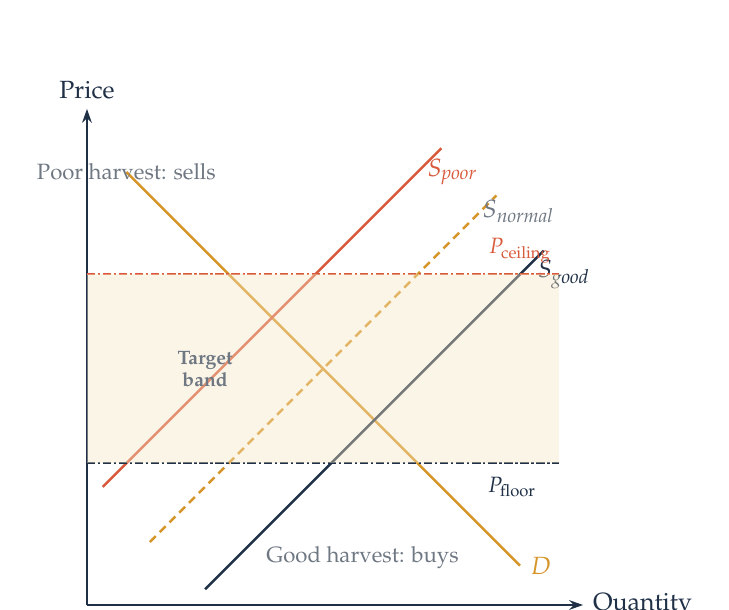
\begin{tikzpicture}[scale=1.0, baseline=(current bounding box.center)]
  % Econ axis
  \draw[econ axis] (0,0)--(6.3,0) node[axis label, right]{Quantity};
  \draw[econ axis] (0,0)--(0,6.3) node[axis label, above]{Price};
  % Demand curve (curve D - stable)
  \draw[curve D] (0.5,5.5)--(5.5,0.5) node[curve label, color=CurveGold, right]{$D$};
  % Supply poor harvest (curve B)
  \draw[curve B] (0.2,1.5)--(4.5,5.8);
  \node[curve label, color=CurveRose, right] at (4.2,5.5) {$S_{\text{poor}}$};
  % Supply good harvest (curve A)
  \draw[curve A] (1.5,0.2)--(5.8,4.5);
  \node[curve label, color=CurveNavy, right] at (5.6,4.2) {$S_{\text{good}}$};
  % Normal supply (curve D shift - dashed)
  \draw[curve D shift] (0.8,0.8)--(5.2,5.2);
  \node[curve label, color=AnnotGray, right] at (4.9,5.0) {$S_{\text{normal}}$};
  % Ceiling price (CurveRose dashed)
  \draw[price floor, color=CurveRose] (0,4.2)--(6.0,4.2);
  \node[annot, color=CurveRose] at (5.5,4.5) {$P_{\text{ceiling}}$};
  % Floor price (CurveNavy dashed)
  \draw[price floor, color=CurveNavy] (0,1.8)--(6.0,1.8);
  \node[annot, color=CurveNavy] at (5.4,1.5) {$P_{\text{floor}}$};
  % Target band shading (FillGold)
  \fill[FillGold,opacity=0.4] (0,1.8) rectangle (6.0,4.2);
  \node[region label, color=AnnotGray, align=center] at (1.5,3.0) {Target\\band};
  % Annotations
  \node[annot, align=left] at (0.5,5.5) {Poor harvest: sells};
  \node[annot, align=left] at (3.5,0.6) {Good harvest: buys};
\end{tikzpicture}%
}{%
\textbf{\color{NavyPrimary}Price Stabilisation}\\[4pt]
$\bullet$ Target price band between floor and ceiling.\\[2pt]
$\bullet$ Poor harvest: supply shifts left;\\[2pt]
\hphantom{$\bullet$ }price rises above ceiling.\\[2pt]
\hphantom{$\bullet$ }Agency sells from buffer stock.\\[2pt]
$\bullet$ Good harvest: supply shifts right;\\[2pt]
\hphantom{$\bullet$ }price falls below floor.\\[2pt]
\hphantom{$\bullet$ }Agency buys surplus.\\[2pt]
\textbf{\color{GoldAccent}Key:} Stabilises prices for farmers\\[2pt]
but costly to maintain.%
}
\end{diagrambox}

\textbf{Challenges:} High storage costs; perishable goods cannot be stored indefinitely; it can be difficult to set the correct price band; scheme requires substantial initial funding.

\subsection{Provision of Information}

Information failures are at the root of both merit and demerit good problems. Governments can intervene with ``soft'' tools that do not directly control prices or quantities:

\begin{itemize}
  \item \textbf{Public information campaigns:} Anti-smoking ads, ``5-a-day'' fruit and vegetable campaigns, drink-driving warnings.
  \item \textbf{Compulsory labelling:} Nutritional information on food packaging, health warnings on cigarettes, energy efficiency labels on appliances.
  \item \textbf{Consumer protection laws:} Requirements for accurate advertising and transparent terms and conditions.
\end{itemize}

By improving information, the government aims to shift demand \emph{away from} demerit goods and \emph{towards} merit goods, without resorting to outright bans or taxes.

\section{Addressing Income and Wealth Inequality}
\begin{tcolorbox}[enhanced,colback=EvalBg,colframe=EvalFrame,arc=0pt,boxrule=1pt,title={\bfseries\color{EvalFrame}Evaluation: Government Microeconomic Intervention},fonttitle=\small]
\small\RaggedRight
\begin{itemize}[itemsep=2pt,topsep=2pt]
  \item \textbf{Maximum price (rent control):} Creates a shortage in the SR, but in the LR developers build less, worsening the shortage further. The \textit{longer-run} effects often outweigh the short-run consumer benefit.
  \item \textbf{Indirect tax effectiveness:} Depends on PED. A tax on tobacco (inelastic demand) raises revenue but barely reduces consumption. On elastic goods, it reduces output substantially. \textit{``To reduce consumption, the good must be price elastic.''}
  \item \textbf{Subsidy as a blunt instrument:} Benefits all consumers, including the wealthy. Targeted vouchers may be more equitable. Subsidies also distort incentives and may sustain inefficient firms.
  \item \textbf{Regulation vs. tax:} For demerit goods, regulation guarantees a reduction in output (e.g.\ a ban). A tax may not reduce consumption if demand is inelastic. However, taxes raise revenue and allow consumer choice.
  \item \textbf{Government failure risk:} Intervention may generate information failure (government lacks local knowledge), political capture, or perverse incentives. The cure can be worse than the disease.
  \item \textbf{Lorenz curve caveat:} The Gini coefficient is a single number that masks \textit{where} inequality is concentrated. Two countries with the same Gini can have very different poverty profiles.
\end{itemize}
\end{tcolorbox}


\subsection{Income as a Flow vs.\ Wealth as a Stock}

\begin{keyterm}{Income}
A \textbf{flow} of money received by an individual or household over a specific \emph{time period} (e.g.\ per month or per year). Sources include wages, rent, interest, and profit. If the source stops, the flow stops.
\end{keyterm}

\begin{keyterm}{Wealth}
A \textbf{stock} of valuable assets owned at a specific \emph{point in time}, including property, savings, shares, and possessions, \emph{minus} any debts. It can grow or shrink independently of current income.
\end{keyterm}

\begin{tcolorbox}[enhanced,colback=LightBlue,colframe=MidBlue!70,arc=0pt,boxrule=0.8pt]
\begin{tabular}{@{}>{\RaggedRight\arraybackslash}p{0.18\linewidth}>{\RaggedRight\arraybackslash}p{0.38\linewidth}>{\RaggedRight\arraybackslash}p{0.38\linewidth}@{}}
& \textbf{\color{NavyPrimary}Income} & \textbf{\color{NavyPrimary}Wealth} \\
\midrule
\textbf{Concept} & Flow & Stock \\
\textbf{Analogy} & A river flowing into a lake & The lake itself \\
\textbf{Measured} & Per time period & At a point in time \\
\textbf{Sources} & Wages, rent, interest, profit & Property, savings, shares, possessions $-$ debts \\
\textbf{Link} & Saving part of your income \emph{builds} your stock of wealth & \\
\end{tabular}
\end{tcolorbox}

\subsection{Measuring Inequality: The Gini Coefficient and Lorenz Curve}

\begin{keyterm}{Gini Coefficient}
A number between \textbf{0} (perfect equality) and \textbf{1} (perfect inequality) that measures the degree of income or wealth inequality in a country. It is derived from the Lorenz curve.
\end{keyterm}

Real-world values: Sweden $\approx 0.25$ (relatively equal); South Africa $\approx 0.60$ (highly unequal).

\begin{diagrambox}[Figure XI -- The Lorenz Curve and Gini Coefficient]
\diagramwithtext{%
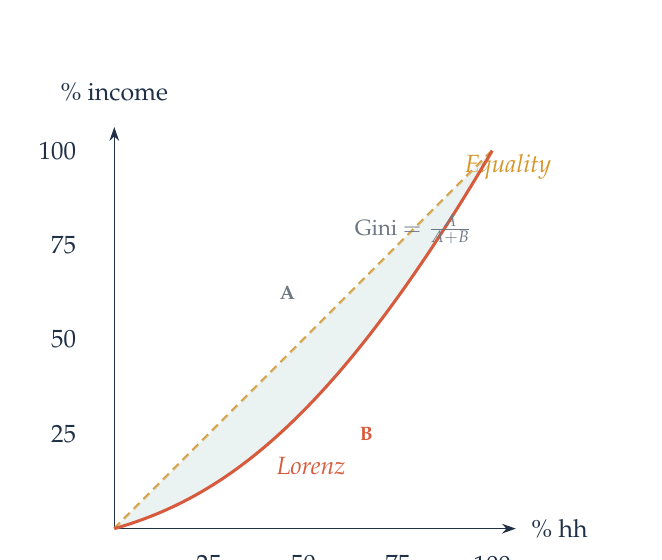
\begin{tikzpicture}[scale=1.0, baseline=(current bounding box.center)]
  \begin{scope}
  \clip (-1.1,-0.6) rectangle (6.6,5.8);

  % Econ axis
  \draw[econ axis] (0,0)--(5.1,0)
        node[axis label, right, xshift=2pt]{\% hh};
  \draw[econ axis] (0,0)--(0,5.1)
        node[axis label, above, yshift=6pt]{\% income};

  % Line of perfect equality (curve D dashed)
  \draw[curve D shift] (0,0)--(4.8,4.8);
  \node[curve label, color=CurveGold] at (5.0,4.6) {Equality};

  % Lorenz curve area (FillPrimary)
  \fill[FillPrimary,opacity=0.5]
        (0,0) .. controls (1.4,0.4) and (2.8,1.4) .. (4.8,4.8)
        -- (0,0) -- cycle;
  % Lorenz curve (curve B)
  \draw[curve B, line width=1.1pt]
        (0,0) .. controls (1.4,0.4) and (2.8,1.4) .. (4.8,4.8);
  \node[curve label, color=CurveRose] at (2.5,0.8) {Lorenz};

  % Area labels
  \node[region label, color=AnnotGray] at (2.2,3.0) {A};
  \node[region label, color=CurveRose] at (3.2,1.2) {B};

  % Gini formula
  \node[annot] at (3.8,3.8) {Gini $= \frac{A}{A+B}$};

  % Tick marks and labels
  \foreach \x/\l in {1.2/25, 2.4/50, 3.6/75, 4.8/100}
    \node[tick label, below, yshift=-2pt] at (\x,-0.15) {\l};
  \foreach \y/\l in {1.2/25, 2.4/50, 3.6/75, 4.8/100}
    \node[tick label, left, xshift=-6pt] at (-0.15,\y) {\l};
  \end{scope}
\end{tikzpicture}%
}{%
\textbf{\color{CurveNavy}Reading the diagram:}\\[4pt]
\textbf{Line of equality:} Bottom 50\% earn exactly 50\% of income.\\[4pt]
\textbf{Lorenz Curve:} Actual distribution. Further from diagonal $=$ more unequal.\\[4pt]
\textbf{Gini:} $\dfrac{\text{Area A}}{\text{Area A + B}}$\\[4pt]
Gini $= 0$: perfect equality\\
Gini $= 1$: perfect inequality%
}
\end{diagrambox}

\subsection{Economic Reasons for Inequality}

\subsubsection{Inequality of Income}

\begin{itemize}
  \item \textbf{Wage differentials:} Differences in skills and education (human capital), productivity, and demand for occupations cause wide pay gaps. A surgeon earns far more than a shop assistant due to years of specialist training.
  \item \textbf{Discrimination:} Gender, racial, or age discrimination generates pay gaps for comparable work.
  \item \textbf{Unemployment:} Those without jobs have zero labour income, creating a stark divide.
  \item \textbf{Unearned income from wealth:} Those who own assets earn rent, interest, and dividends without working -- widening the gap between asset owners and those with none.
  \item \textbf{Market power:} Owners of dominant firms extract large profits; workers in competitive labour markets earn the minimum.
  \item \textbf{Globalisation and technology:} ``Winner-takes-all'' markets and automation reduce demand for low-skilled labour, depressing wages at the bottom.
\end{itemize}

\subsubsection{Inequality of Wealth}

\begin{itemize}
  \item \textbf{Inheritance:} Wealth transferred across generations entrenches existing concentrations in certain families.
  \item \textbf{Compounding effect of existing wealth:} Asset ownership generates income (dividends, rent) that can purchase more assets, accelerating wealth accumulation.
  \item \textbf{Asset appreciation:} Property and share values tend to rise over time, automatically increasing the wealth of existing owners.
  \item \textbf{Differential saving propensities:} High-income earners save and invest a larger share of income; low-income earners spend almost all income on necessities and cannot build wealth.
  \item \textbf{Life-cycle effects:} Wealth naturally concentrates in older age groups who have had longer to accumulate it.
\end{itemize}

\subsection{Policies to Redistribute Income and Wealth}

\begin{tcolorbox}[enhanced,colback=LightBlue,colframe=MidBlue!70,arc=0pt,boxrule=0.8pt]
\begin{tabular}{@{}>{\RaggedRight\arraybackslash}p{0.24\linewidth}>{\RaggedRight\arraybackslash}p{0.35\linewidth}>{\RaggedRight\arraybackslash}p{0.37\linewidth}@{}}
\textbf{\color{NavyPrimary}Policy} & \textbf{\color{NavyPrimary}How it Works} & \textbf{\color{NavyPrimary}Evaluation} \\
\midrule
\textbf{Minimum Wage} & Legal wage floor raises income for lowest-paid workers. & \textit{Pro:} Raises living standards. \textit{Con:} May cause unemployment if set above equilibrium. \\
\textbf{Transfer Payments} & One-way government payments (benefits, pensions, child support) to those without labour income. & Provides a safety net but may reduce incentives to work. \\
\textbf{Progressive Income Tax} & Higher earners pay a greater \% of income. Revenue funds public services and benefits. & Reduces disposable income inequality; may reduce work incentives at high rates. \\
\textbf{Inheritance \& Capital Taxes} & Tax on wealth transfers (inheritance tax) and asset gains (capital gains tax). & Directly reduces wealth concentration; but may discourage saving and investment. \\
\textbf{State Provision of Services} & Free education, healthcare, housing. Raises real standard of living without cash transfers. & Highly effective for equity; costly to fund; quality depends on political will. \\
\end{tabular}
\end{tcolorbox}

\begin{example}[Progressive Taxation in Practice]
Under a typical progressive income tax system:
\begin{itemize}
  \item First \pounds12{,}500 of income: 0\% tax (personal allowance)
  \item \pounds12{,}501 to \pounds50{,}000: 20\% tax
  \item Over \pounds50{,}000: 40\% tax
\end{itemize}
A worker earning \pounds20{,}000 pays 20\% on \pounds7{,}500 $=$ \pounds1{,}500. A worker earning \pounds100{,}000 pays 0\% + 20\% + 40\% on successively higher bands, paying a far higher total and average tax rate. The government uses this revenue to fund transfer payments and public services, redistributing real income downward.
\end{example}

\section{Exam Practice Questions -- Chapter 3}

\begin{exampractice}
\begin{enumerate}[leftmargin=*]

\item \textbf{``Evaluate the effectiveness of indirect taxation as a means of correcting negative externalities in the market for demerit goods such as cigarettes.''} [15 marks]

\textit{Model structure: Define externality and demerit good $\to$ Draw S and D diagram showing market equilibrium at over-consumption relative to the social optimum $\to$ Show how a tax shifts supply up (or demand down), reducing Q and raising price $\to$ Effectiveness depends on: (1) PED of demand — if very inelastic, tax barely reduces consumption; if elastic, consumption falls sharply; (2) magnitude of externality — if external cost is large, a small tax is insufficient $\to$ Evaluate: tax raises government revenue (good for redistribution), but is regressive (hits poor consumers harder as a \% of income); tax allows consumer choice (unlike a ban) but is slow to take effect and depends on price sensitivity $\to$ Discuss alternatives: regulation/ban (guaranteed reduction but removes choice), information campaigns (cheaper but may be ineffective if consumers are addicted or have time-inconsistent preferences) $\to$ Conclude: effectiveness depends heavily on PED and whether the goal is revenue collection vs. consumption reduction.}

\item \textbf{``Using supply and demand diagrams, analyse the effects of a government subsidy on the market for a merit good, and discuss the extent to which it achieves its intended objectives.''} [15 marks]

\textit{Model structure: Define merit good and explain under-consumption due to information failure $\to$ Draw initial S and D at under-optimal Q $\to$ Show subsidy shifts supply curve right (or reduces effective price to consumers) $\to$ Analysis: quantity rises (toward social optimum), price to consumers falls $\to$ Intended objectives: increase consumption and access, reduce inequality (if targeted), correct information failure $\to$ Evaluate: (1) cost to government = subsidy $\times$ Q, can be large; (2) deadweight loss removed (surplus increases) if subsidy correctly sized to internalise positive externality; (3) risk of over-subsidy leading to over-consumption; (4) distributional issue: universal subsidies benefit the wealthy as much as the poor (regressive in total spending, though progressive as a \% of income for those at the bottom); targeted subsidies via vouchers are more equitable but administratively complex $\to$ Real example: NHS provides free healthcare (perfect subsidy = 100\%); subsidised childcare helps working parents but misses non-workers $\to$ Conclude: subsidy effectiveness depends on whether information failure is the true cause of under-consumption, and whether the benefit reaches intended recipients.}

\item \textbf{``Compare maximum price controls (price ceilings) with minimum prices (price floors) as tools of government intervention, using supply and demand analysis and discussing unintended consequences.''} [15 marks]

\textit{Model structure: Draw separate diagrams for each $\to$ Maximum price: sets a binding ceiling below equilibrium P, causing shortage (Qd $>$ Qs), non-price rationing (queuing, waiting lists, corruption), reduced quality (suppliers cut corners), black markets $\to$ Minimum price: sets a floor above equilibrium P, causing surplus (Qs $>$ Qd), government must buy up surplus (costly) or firms destroy output (wasteful), protects inefficient high-cost producers $\to$ Unintended consequences: (1) both distort incentives — ceiling discourages supply, floor discourages demand; (2) both create deadweight loss (reduced surplus); (3) both require enforcement (black markets, illegal undercutting); (4) both have distributional effects (ceiling helps consumers short-term but harms them long-term if supply shrinks; floor helps producers but harms consumers) $\to$ Real examples: rent control (housing shortage worsens long-run); minimum wage (modest employment loss if not too high above equilibrium); agricultural price floors (EU, Japan — enormous surpluses and fiscal cost) $\to$ Compare to tax/subsidy: price controls specify quantity indirectly; tax/subsidy control quantity directly and raise revenue or cost money but don't create persistent shortages/surpluses $\to$ Conclude: price controls are blunt instruments; they work temporarily but cause worsening distortions if conditions change and the control price becomes increasingly binding.}

\item \textbf{``Analyse the extent to which government intervention in markets can reduce income and wealth inequality without reducing economic efficiency.''} [15 marks]

\textit{Model structure: Explain the equity-efficiency trade-off: redistribution (taxes, transfers) improves equity but may reduce efficiency by discouraging work and investment $\to$ Analyse different intervention types: (1) progressive income tax — reduces disposable inequality but may reduce labour supply (empirical evidence suggests modest effect); (2) transfer payments — target the poorest but may create welfare traps (lose benefits if earnings rise, so marginal tax rates are very high); (3) inheritance tax — targets wealth but easy to evade; (4) state provision of services (education, healthcare) — improves access for poor without taxing earnings, so minimal work-disincentive effect $\to$ Show that the trade-off is NOT absolute: (1) some interventions (e.g., early-childhood education subsidy) may increase both equity and long-run growth (reduces inequality AND boosts human capital); (2) redistribution funded by taxes on land (inelastic supply) or pollution (corrects externality) may reduce DWL rather than increase it $\to$ Empirical evidence: Nordic countries have high taxes and transfers, yet good growth and innovation (education subsidies, R\&D support); tight inequality may improve growth by boosting aggregate demand and reducing crime/social instability $\to$ Discuss limits: very high marginal tax rates (>80\%) likely reduce growth; means-tested benefits create poverty traps; state monopolies in service provision may reduce quality $\to$ Conclude: the equity-efficiency trade-off is real but not inevitable; it depends on policy design (targeted vs. universal transfers, supply-side vs. demand-side redistribution) and context (how elastic are labour supply and capital mobility?).}

\item \textbf{``Evaluate the claim that ``perfect equality of income and wealth is neither desirable nor achievable in a market economy.''''} [15 marks]

\textit{Model structure: Define perfect equality $\to$ Argue it is undesirable: (1) undermines incentives to work, invest, and innovate (levelling everyone to the bottom); (2) violates liberty (requires constant confiscatory taxation); (3) does not account for differences in preferences (some want leisure, some want income; forced equality overrides both); (4) even communist regimes failed to achieve it — instead created inequality of power and status $\to$ Argue it is unachievable: (1) humans have different talents and effort levels; equal income would require equal productivity, which is impossible; (2) capital ownership compounds wealth; (3) luck and circumstance create randomness that markets amplify $\to$ Counter-arguments: (1) desirability claim ignores that extreme inequality may be even worse than forced equality (social instability, reduced aggregate welfare); (2) achievability claim conflates "perfect" equality with "reduced" inequality — the latter is both desirable and achievable $\to$ Discuss the real goal: not perfect equality but reduced \emph{unnecessary} inequality (from discrimination, information failure, inherited advantage) while preserving incentive-driven inequality $\to$ Real examples: Nordic redistribution aims for high marginal tax rates (70\%) at top but allows substantial inequality; eliminates extreme poverty but tolerates income ratios of 10:1 or more $\to$ Conclude: perfect equality is neither desirable nor achievable, but significant reduction in inequality IS possible and worth pursuing if done carefully to avoid killing incentives.}

\end{enumerate}
\end{exampractice}

% ============================================================
%  CHAPTER 4: THE MACROECONOMY
% ============================================================
\chapter{The Macroeconomy}

\section{National Income Statistics}

\subsection{Meaning of National Income}

\begin{coreidea}
National income is the total value of all goods and services produced by a country's economy over a specific period -- usually one year. It measures the country's overall economic activity and is the primary indicator of living standards.
\end{coreidea}

Just as personal income sums up your salary, bonuses, and other earnings, national income adds up the value created by every business, farm, factory, and service provider in the country.

\subsection{Measurement of National Income}

There are three interconnected measures, each approaching the same total from a different angle.

\subsubsection{1. Gross Domestic Product (GDP)}

\begin{keyterm}{GDP}
The total \textbf{market value of all final goods and services produced within a country's borders} in a given time period, regardless of who owns the factors of production.
\end{keyterm}

\begin{itemize}
  \item \textbf{Domestic:} What is produced \emph{inside} the country. A Japanese-owned car factory in the UK counts towards UK GDP.
  \item \textbf{Final goods:} Only the value of the finished product is counted to avoid \emph{double-counting} (the steel sold to a car maker is not counted again when the car is sold).
  \item \textbf{Gross:} Does not deduct wear and tear on capital (depreciation).
\end{itemize}

GDP can be measured three ways -- all should give the same result:

\begin{tcolorbox}[enhanced,colback=LightBlue,colframe=MidBlue!70,arc=0pt,boxrule=0.8pt]
\begin{tabular}{@{}>{\RaggedRight\arraybackslash}p{0.22\linewidth}>{\RaggedRight\arraybackslash}p{0.73\linewidth}@{}}
\textbf{\color{NavyPrimary}Method} & \textbf{\color{NavyPrimary}What it Does} \\
\midrule
\textbf{Expenditure} & Adds all spending: GDP $= C + I + G + (X - M)$ \\
\textbf{Income} & Adds all factor incomes: wages $+$ rent $+$ interest $+$ profit \\
\textbf{Output} & Sums value-added by each sector (primary, secondary, tertiary) \\
\end{tabular}
\end{tcolorbox}

\subsubsection{2. Gross National Income (GNI)}

\begin{keyterm}{GNI}
The total income earned by a country's \textbf{citizens and businesses worldwide}, regardless of where production takes place.
\[
\text{GNI} = \text{GDP} + \text{Net Property Income from Abroad}
\]
Net property income from abroad $=$ (income earned by domestic factors abroad) $-$ (income earned by foreign factors domestically).
\end{keyterm}

\begin{example}[GNI vs GDP]
Profits repatriated to the UK by a British-owned firm in India are \emph{added} to GDP to get GNI. Profits repatriated to the USA by an American-owned firm operating in the UK are \emph{subtracted}.
\end{example}

\subsubsection{3. Net National Income (NNI)}

\begin{keyterm}{NNI}
GNI adjusted for \textbf{depreciation} (capital consumption) -- the value of capital worn out during production.
\[
\text{NNI} = \text{GNI} - \text{Depreciation}
\]
NNI is often considered the most meaningful measure of \emph{sustainable} national income, as it shows what the country earns after maintaining its existing capital stock.
\end{keyterm}

\subsection{Market Prices vs.\ Basic Prices}

\begin{tcolorbox}[enhanced,colback=LightBlue,colframe=MidBlue!70,arc=0pt,boxrule=0.8pt]
\begin{tabular}{@{}>{\RaggedRight\arraybackslash}p{0.25\linewidth}>{\RaggedRight\arraybackslash}p{0.70\linewidth}@{}}
\textbf{\color{NavyPrimary}Price Basis} & \textbf{\color{NavyPrimary}What it Includes} \\
\midrule
\textbf{Market Prices} & The price the consumer pays, \emph{including} indirect taxes and \emph{excluding} subsidies. \\
\textbf{Basic Prices (Factor Cost)} & The price received by the producer, \emph{excluding} indirect taxes and \emph{including} subsidies. \\
\end{tabular}
\end{tcolorbox}

\[
\text{GDP at Factor Cost} = \text{GDP at Market Prices} - \text{Indirect Taxes} + \text{Subsidies}
\]

\begin{example}[Bread Loaf]
Market price $= \pounds1.20$ (includes $\pounds0.20$ VAT). Government subsidy to baker $= \pounds0.05$.\\
Basic Price $= \pounds1.20 - \pounds0.20 + \pounds0.05 = \pounds1.05$.
\end{example}

\subsection{Gross vs.\ Net Values}

Subtracting \textbf{depreciation} from any gross measure gives the net equivalent:

\begin{tcolorbox}[enhanced,colback=LightBlue,colframe=MidBlue!70,arc=0pt,boxrule=0.8pt]
\begin{tabular}{@{}>{\RaggedRight\arraybackslash}p{0.42\linewidth}>{\RaggedRight\arraybackslash}p{0.53\linewidth}@{}}
\textbf{\color{NavyPrimary}Gross Measure} & \textbf{\color{NavyPrimary}Net Equivalent} \\
\midrule
GDP (Gross Domestic Product) & NDP $=$ GDP $-$ Depreciation \\
GNI (Gross National Income) & NNI $=$ GNI $-$ Depreciation \\
\end{tabular}
\end{tcolorbox}

\begin{evaluation}{GDP as a Measure of Living Standards}
\textbf{Strengths / Arguments For:}
\begin{itemize}[leftmargin=*, nosep]
\item Directly measures the output of goods and services available to the population.
\item Enables comparison of economic performance across time and between countries.
\item Real GDP per capita adjusts for both inflation and population changes.
\item Easy to calculate and communicate to policymakers and the public.
\end{itemize}
\textbf{Limitations / Arguments Against:}
\begin{itemize}[leftmargin=*, nosep]
\item Does not account for income distribution; a country with high GDP but unequal incomes may have lower average living standards for the majority.
\item Ignores non-market activities (housework, volunteer work, care for family members) that contribute to welfare.
\item Does not deduct environmental damage, resource depletion, or carbon emissions.
\item Counts ``bads'' as goods: increased spending on healthcare or pollution cleanup raises GDP but signals a social problem.
\item Leisure time is not measured, yet it is a crucial component of well-being.
\end{itemize}
\textbf{It depends on\ldots}
\begin{itemize}[leftmargin=*, nosep]
\item The distribution of income; GDP per capita is more meaningful in equal societies.
\item Environmental sensitivity; nations with high resource extraction may show high growth but declining well-being.
\item Development stage; GDP matters more in poor countries (food and shelter) than in rich ones (where marginal utility of income is lower).
\end{itemize}
\end{evaluation}

\section{The Circular Flow of Income}

\begin{coreidea}
The circular flow model shows how money, goods, and services flow continuously between households, firms, the government, and the rest of the world. Your spending is someone else's income -- and their spending becomes yours.
\end{coreidea}

\subsection{The Circular Flow}

\subsubsection{Closed Economy (Two-Sector Model)}

In a simplified economy with only households and firms:
\begin{itemize}
  \item \textbf{Real flow:} Households provide labour, land, and capital to firms; firms provide goods and services to households.
  \item \textbf{Money flow} (opposite direction): Firms pay wages, rent, and profit to households; households pay for goods and services from firms.
\end{itemize}

\subsubsection{Open Economy (Four-Sector Model)}

A realistic economy adds the \textbf{government} and the \textbf{international sector}:

\begin{tcolorbox}[enhanced,colback=LightBlue,colframe=MidBlue!70,arc=0pt,boxrule=0.8pt]
\begin{tabular}{@{}>{\RaggedRight\arraybackslash}p{0.22\linewidth}>{\RaggedRight\arraybackslash}p{0.73\linewidth}@{}}
\textbf{\color{NavyPrimary}Connection} & \textbf{\color{NavyPrimary}Flow} \\
\midrule
Households $\leftrightarrow$ Govt & Households pay taxes (T); Govt pays transfer payments (benefits, pensions). \\
Firms $\leftrightarrow$ Govt & Firms pay taxes; Govt buys goods/services through Government Spending (G). \\
Domestic $\leftrightarrow$ World & Imports (M) flow spending out; Exports (X) bring spending in. \\
\end{tabular}
\end{tcolorbox}

\subsection{Injections and Leakages}

\begin{keyterm}{Injections (J)}
\textbf{Additions} of new spending into the circular flow that do not come from current household income: \textbf{Investment (I)}, \textbf{Government Spending (G)}, and \textbf{Exports (X)}.
\[
J = I + G + X
\]
\end{keyterm}

\begin{keyterm}{Leakages / Withdrawals (W)}
\textbf{Removals} of spending from the circular flow -- income that is not spent on domestic goods and services: \textbf{Savings (S)}, \textbf{Taxation (T)}, and \textbf{Imports (M)}.
\[
W = S + T + M
\]
\end{keyterm}

\subsection{Equilibrium and Disequilibrium}

\begin{tcolorbox}[enhanced,colback=LightBlue,colframe=MidBlue!70,arc=0pt,boxrule=0.8pt]
\begin{tabular}{@{}>{\RaggedRight\arraybackslash}p{0.22\linewidth}>{\RaggedRight\arraybackslash}p{0.35\linewidth}>{\RaggedRight\arraybackslash}p{0.38\linewidth}@{}}
\textbf{\color{NavyPrimary}Condition} & \textbf{\color{NavyPrimary}Meaning} & \textbf{\color{NavyPrimary}Result} \\
\midrule
$J = W$ & New spending in $=$ spending out & National income \textbf{stable} \\
$J > W$ & More injected than withdrawn & National income \textbf{rises} \\
$J < W$ & More withdrawn than injected & National income \textbf{falls} \\
\end{tabular}
\end{tcolorbox}

\section{Aggregate Demand and Aggregate Supply}

\subsection{Aggregate Demand: Definition and Components}

\begin{keyterm}{Aggregate Demand (AD)}
The \textbf{total planned spending} on goods and services produced within an economy at a given overall price level over a given period.
\[
AD = C + I + G + (X - M)
\]
\end{keyterm}

\begin{tcolorbox}[enhanced,colback=LightBlue,colframe=MidBlue!70,arc=0pt,boxrule=0.8pt]
\begin{tabular}{@{}>{\RaggedRight\arraybackslash}p{0.08\linewidth}>{\RaggedRight\arraybackslash}p{0.17\linewidth}>{\RaggedRight\arraybackslash}p{0.68\linewidth}@{}}
\textbf{\color{NavyPrimary}} & \textbf{\color{NavyPrimary}Component} & \textbf{\color{NavyPrimary}Description} \\
\midrule
\textbf{C} & Consumption & Household spending on goods and services. The \emph{largest} component in most economies. \\
\textbf{I} & Investment & Firm spending on capital goods (machinery, factories). \emph{Not} buying stocks and shares. \\
\textbf{G} & Govt Spending & Govt spending on public services. Does \emph{not} include transfer payments (pensions, benefits). \\
\textbf{X$-$M} & Net Exports & Exports minus imports. Positive if trade surplus; negative if trade deficit. \\
\end{tabular}
\end{tcolorbox}

\subsection{The AD Curve: Shape, Determinants, and Shifts}

\subsubsection{Why the AD Curve is Downward-Sloping}

\begin{itemize}
  \item \textbf{Wealth (Real Balance) Effect:} Lower price level $\Rightarrow$ greater purchasing power $\Rightarrow$ more consumption.
  \item \textbf{Interest Rate Effect:} Lower price level $\Rightarrow$ less demand for money $\Rightarrow$ lower interest rates $\Rightarrow$ more C and I.
  \item \textbf{International Trade Effect:} Lower domestic prices $\Rightarrow$ exports more competitive, imports less attractive $\Rightarrow$ (X$-$M) rises.
\end{itemize}

\subsubsection{Causes of Shifts in AD}

\begin{tcolorbox}[enhanced,colback=LightBlue,colframe=MidBlue!70,arc=0pt,boxrule=0.8pt]
\begin{tabular}{@{}>{\RaggedRight\arraybackslash}p{0.46\linewidth}>{\RaggedRight\arraybackslash}p{0.49\linewidth}@{}}
\textbf{\color{NavyPrimary}AD Increases (Rightward Shift)} & \textbf{\color{NavyPrimary}AD Decreases (Leftward Shift)} \\
\midrule
Cut in interest rates & Rise in interest rates \\
Rise in consumer/business confidence & Fall in consumer/business confidence \\
Currency depreciation & Currency appreciation \\
Increase in government spending & Decrease in government spending \\
Income or corporation tax cut & Income or corporation tax rise \\
\end{tabular}
\end{tcolorbox}

\begin{diagrambox}[Figure XII -- The AD/AS Model: Equilibrium and Shifts]
\diagramwithtext{%
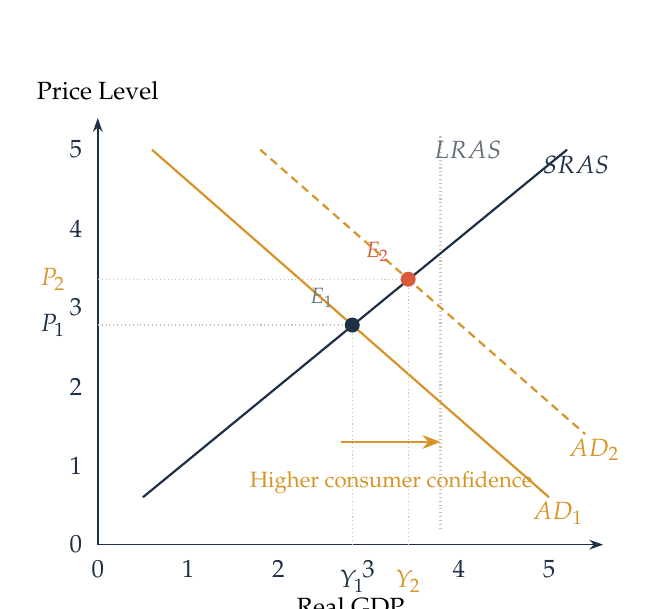
\begin{tikzpicture}[scale=1.0, baseline=(current bounding box.center)]
  \begin{axis}[econ chart,
    xlabel style={at={(ticklabel cs:0.5)}, anchor=north}, width=8cm, height=7cm, xmin=0, xmax=5.6, ymin=0, ymax=5.4,
    xlabel={\small Real GDP},
    ylabel={\small Price Level}]
    % LRAS (vertical)
    \addplot[guide line, very thick] coordinates {(3.8,0.2)(3.8,5.2)};
    \node[curve label, AxisCharcoal!70] at (4.1,5.0) {$LRAS$};

    % SRAS (upward sloping)
    \addplot[curve A, thick] coordinates {(0.5,0.6)(5.2,5.0)};
    \node[curve label, CurveNavy] at (5.3,4.8) {$SRAS$};

    % AD1 (original)
    \addplot[curve accent, thick] coordinates {(0.6,5.0)(5.0,0.6)};
    \node[curve label, CurveGold] at (5.1,0.4) {$AD_1$};

    % AD2 (shifted right)
    \addplot[curve accent shift, thick] coordinates {(1.8,5.0)(5.4,1.4)};
    \node[curve label, CurveGold] at (5.5,1.2) {$AD_2$};

    % Equilibrium E1
    % SRAS: y = 0.936x + 0.132; AD1: y = -x + 5.6 → x=2.82, y=2.78
    \addplot[econ point, mark=*] coordinates {(2.82,2.78)};
    \node[annot, above left] at (2.72,2.88) {$E_1$};
    \addplot[guide projection] coordinates {(2.82,0)(2.82,2.78)};
    \node[tick label, below] at (2.82,-0.2) {$Y_1$};
    \addplot[guide projection] coordinates {(0,2.78)(2.82,2.78)};
    \node[tick label, left] at (-0.25,2.78) {$P_1$};

    % Equilibrium E2
    % SRAS: y = 0.936x + 0.132; AD2: y = -x + 6.8 → x=3.44, y=3.36
    \addplot[econ point accent, mark=*] coordinates {(3.44,3.36)};
    \node[annot accent, above left] at (3.34,3.46) {$E_2$};
    \addplot[guide projection] coordinates {(3.44,0)(3.44,3.36)};
    \node[tick label, CurveGold, below] at (3.44,-0.2) {$Y_2$};
    \addplot[guide projection] coordinates {(0,3.36)(3.44,3.36)};
    \node[tick label, CurveGold, left] at (-0.25,3.36) {$P_2$};

    % Shift arrow labeled with cause
    \draw[-{Stealth}, CurveGold, thick] (2.7,1.3)--(3.8,1.3);
    \node[annot, CurveGold, below] at (3.25,1.05) {Higher consumer confidence};
  \end{axis}
\end{tikzpicture}%

}{%
\textbf{\color{NavyPrimary}AD increases (AD\textsubscript{1} $\to$ AD\textsubscript{2}):}\\[4pt]
$\bullet$ Real output rises: Y\textsubscript{1} $\to$ Y\textsubscript{2}\\[2pt]
$\bullet$ Price level rises: P\textsubscript{1} $\to$ P\textsubscript{2}\\[2pt]
$\bullet$ Employment rises\\[6pt]
\textbf{\color{NavyPrimary}LRAS (vertical):}\\[2pt]
Full employment output. Long run = price adjusts, output returns here.\\[6pt]
\textbf{\color{GoldAccent}Key:} AD shifts cause both output and price changes in short run.%
}
\end{diagrambox}

\begin{evaluation}{Demand-Pull vs. Cost-Push Inflation}
\textbf{Strengths of Demand-Pull Model:}
\begin{itemize}[leftmargin=*, nosep]
\item Occurs when economy is at or near full employment; money and spending grow faster than productive capacity.
\item Contractionary policy (higher interest rates, reduced government spending) directly targets the root cause.
\item Easier to diagnose: look for AD pressure and tight labour markets.
\end{itemize}
\textbf{Strengths of Cost-Push Model:}
\begin{itemize}[leftmargin=*, nosep]
\item Explains ``stagflation'' (rising prices and falling output), which demand-pull theory cannot.
\item Can occur at any level of output; does not require full employment.
\item Policy response is more nuanced: tightening demand worsens output, while loosening it worsens inflation.
\end{itemize}
\textbf{Limitations and Trade-offs:}
\begin{itemize}[leftmargin=*, nosep]
\item Real inflation is usually mixed; both demand and cost factors play a role, making diagnosis difficult.
\item If you misidentify the cause, policy response will backfire (contractionary policy worsens cost-push inflation by reducing output).
\item Supply-side policies take years to work; in the short run, cost-push inflation may require accepting higher unemployment (a harsh trade-off).
\end{itemize}
\textbf{It depends on\ldots}
\begin{itemize}[leftmargin=*, nosep]
\item The output gap; if large spare capacity exists, inflation is likely demand-pull.
\item International factors; oil price shocks or currency depreciation often trigger cost-push inflation regardless of domestic demand.
\item Central bank credibility; if inflation expectations are anchored, even cost-push shocks may not trigger a wage-price spiral.
\end{itemize}
\end{evaluation}

\subsection{Aggregate Supply: SRAS and LRAS}

\begin{keyterm}{Aggregate Supply (AS)}
The total planned output of all firms in an economy at a given overall price level over a given period.
\end{keyterm}

\subsubsection{Short Run Aggregate Supply (SRAS)}

The SRAS curve is \textbf{upward-sloping} because, in the short run, some factor costs (especially wages) are sticky and fixed by contracts. When the price level rises but wages stay fixed, profit margins widen, incentivising firms to increase output.

\textbf{Causes of a shift in SRAS:}
\begin{itemize}
  \item \textbf{Rightward (increase):} Fall in raw material prices (e.g.\ oil), fall in wages, cut in indirect taxes, government subsidies to firms.
  \item \textbf{Leftward (decrease):} Rise in oil prices, higher wages, rise in indirect taxes, weaker exchange rate (makes imported inputs costlier).
\end{itemize}

\subsubsection{Long Run Aggregate Supply (LRAS)}

The LRAS curve is \textbf{vertical} at the economy's \emph{full employment output}. In the long run, the price level does not affect productive capacity -- output depends only on the quantity and quality of factors of production.

\textbf{Causes of a shift in LRAS (changes to productive potential):}
\begin{itemize}
  \item Investment in new capital and technology.
  \item Improved education, training, and healthcare (human capital).
  \item Discovery of new natural resources.
  \item Growth of the labour force (immigration, higher participation rate).
  \item Improved institutions, infrastructure, and efficiency.
\end{itemize}

\subsection{Equilibrium and Effects of Shifts}

\begin{tcolorbox}[enhanced,colback=LightBlue,colframe=MidBlue!70,arc=0pt,boxrule=0.8pt]
\begin{tabular}{@{}>{\RaggedRight\arraybackslash}p{0.25\linewidth}>{\RaggedRight\arraybackslash}p{0.22\linewidth}>{\RaggedRight\arraybackslash}p{0.22\linewidth}>{\RaggedRight\arraybackslash}p{0.22\linewidth}@{}}
\textbf{\color{NavyPrimary}Change} & \textbf{\color{NavyPrimary}Output} & \textbf{\color{NavyPrimary}Price Level} & \textbf{\color{NavyPrimary}Employment} \\
\midrule
AD rises (rightward) & Rises & Rises & Rises \\
AD falls (leftward) & Falls & Falls & Falls \\
AS rises (rightward) & Rises & \textbf{Falls} & Rises \\
AS falls (leftward) & Falls & \textbf{Rises} & Falls \\
\midrule
Both AD and AS rise & Definitely rises & \textbf{Ambiguous} & Rises \\
AD rises, AS falls & \textbf{Ambiguous} & Definitely rises & Ambiguous \\
\end{tabular}
\end{tcolorbox}

\begin{tcolorbox}[enhanced,colback=LightGold,colframe=GoldAccent,arc=0pt,boxrule=0.9pt,
  left=8pt,right=8pt,top=6pt,bottom=6pt]
\textbf{\color{NavyPrimary}Stagflation:} A fall in AS (leftward shift) causes output to \emph{fall} and prices to \emph{rise} simultaneously -- the worst of both worlds. This occurred during the 1970s oil price shocks.
\end{tcolorbox}

\begin{evaluation}{The AD/AS Model: Classical vs. Keynesian Perspectives}
\textbf{Strengths / Arguments For:}
\begin{itemize}[leftmargin=*, nosep]
\item Unifies microeconomic (supply and demand) and macroeconomic thinking in one framework.
\item Can illustrate both demand-pull and cost-push inflation mechanisms; different policy responses for each.
\item The vertical LRAS correctly reflects long-run growth constraints; the upward SRAS captures short-run nominal rigidities.
\end{itemize}
\textbf{Limitations / Arguments Against:}
\begin{itemize}[leftmargin=*, nosep]
\item Assumes a smooth production possibility frontier; in reality, economies face unemployment and slack capacity that are not fully captured.
\item The SRAS slope depends critically on wage flexibility; if wages are very sticky, the model may overstate the economy's ability to produce extra output at higher prices.
\item Does not model financial instability, credit constraints, or balance sheet effects that are crucial in recessions.
\end{itemize}
\textbf{It depends on\ldots}
\begin{itemize}[leftmargin=*, nosep]
\item Time horizon; the model works well for short-term cyclical analysis but less well for long-term growth.
\item Wage-setting institutions; in countries with strong unions and wage-setting floors, the SRAS may be steeper (less responsive to prices).
\item Credibility of monetary policy; if inflation expectations are anchored, the short-run trade-off between output and prices is more favourable.
\end{itemize}
\end{evaluation}

\section{Economic Growth}

\subsection{Definition and Measurement}

\begin{keyterm}{Economic Growth}
A \textbf{sustained increase in the productive capacity of an economy}, measured as the annual percentage change in \textbf{real GDP}.
\[
\text{Growth Rate} = \frac{\text{Real GDP}_{\text{Year 2}} - \text{Real GDP}_{\text{Year 1}}}{\text{Real GDP}_{\text{Year 1}}} \times 100
\]
\end{keyterm}

\begin{example}[Calculating Growth]
Real GDP was \pounds1 trillion in 2022 and \pounds1.03 trillion in 2023.\\
Growth rate $= \frac{1.03 - 1.00}{1.00} \times 100 = \mathbf{3\%}$
\end{example}

\subsection{Nominal GDP vs.\ Real GDP}

\begin{tcolorbox}[enhanced,colback=LightBlue,colframe=MidBlue!70,arc=0pt,boxrule=0.8pt]
\begin{tabular}{@{}>{\RaggedRight\arraybackslash}p{0.22\linewidth}>{\RaggedRight\arraybackslash}p{0.37\linewidth}>{\RaggedRight\arraybackslash}p{0.37\linewidth}@{}}
& \textbf{\color{NavyPrimary}Nominal GDP} & \textbf{\color{NavyPrimary}Real GDP} \\
\midrule
\textbf{Prices used} & Current year prices & Constant base year prices \\
\textbf{Adjusted for inflation?} & No & Yes \\
\textbf{What it shows} & Changes in output \emph{and} prices & Changes in \emph{actual output} only \\
\textbf{Use} & Face value measure & True growth measure \\
\end{tabular}
\end{tcolorbox}

\[
\text{Real GDP} = \frac{\text{Nominal GDP}}{\text{GDP Deflator}} \times 100
\]

\begin{example}[Real GDP Calculation]
Nominal GDP $= \pounds1{,}500$ bn. GDP Deflator $= 125$ (base year $= 100$).\\
Real GDP $= \frac{1{,}500}{125} \times 100 = \pounds\mathbf{1{,}200}$ \textbf{billion} at base year prices.
\end{example}

\subsection{Causes of Economic Growth}

\begin{tcolorbox}[enhanced,colback=LightBlue,colframe=MidBlue!70,arc=0pt,boxrule=0.8pt]
\begin{tabular}{@{}>{\RaggedRight\arraybackslash}p{0.35\linewidth}>{\RaggedRight\arraybackslash}p{0.60\linewidth}@{}}
\textbf{\color{NavyPrimary}Source} & \textbf{\color{NavyPrimary}Examples} \\
\midrule
\textbf{More resources} (quantity) & New resource discoveries; larger labour force (immigration, participation); more capital investment \\
\textbf{Better resources} (quality) & Technological progress; higher human capital (education, training); improved infrastructure and institutions \\
\end{tabular}
\end{tcolorbox}

\subsection{Benefits and Costs of Economic Growth}

\begin{tcolorbox}[enhanced,colback=LightBlue,colframe=MidBlue!70,arc=0pt,boxrule=0.8pt]
\begin{tabular}{@{}>{\RaggedRight\arraybackslash}p{0.46\linewidth}>{\RaggedRight\arraybackslash}p{0.49\linewidth}@{}}
\textbf{\color{NavyPrimary}Benefits} & \textbf{\color{NavyPrimary}Costs} \\
\midrule
Higher real incomes and living standards & Inflationary pressure (demand-pull) \\
More jobs; lower unemployment & Environmental damage: pollution, resource depletion, carbon emissions \\
Higher tax revenues for public services & Inequality: benefits may go mainly to the wealthy \\
Higher business profits; more investment & Congestion and negative externalities \\
Can fund welfare and reduce poverty & Worsening current account (more imports demanded) \\
\end{tabular}
\end{tcolorbox}

\section{Unemployment}

\subsection{Definition of Unemployment}

\begin{keyterm}{Unemployment}
A person is unemployed if they are \textbf{able, available, and actively seeking work} at current wage rates but are unable to find a job.
\end{keyterm}

\subsection{Measurement and Difficulties}

\[
\text{Unemployment Rate} = \frac{\text{Number Unemployed}}{\text{Labour Force}} \times 100
\]

Where: Labour Force $=$ Employed $+$ Unemployed (actively seeking work).

\begin{tcolorbox}[enhanced,colback=LightBlue,colframe=MidBlue!70,arc=0pt,boxrule=0.8pt]
\begin{tabular}{@{}>{\RaggedRight\arraybackslash}p{0.30\linewidth}>{\RaggedRight\arraybackslash}p{0.65\linewidth}@{}}
\textbf{\color{NavyPrimary}Difficulty} & \textbf{\color{NavyPrimary}Effect on the Measured Rate} \\
\midrule
\textbf{Discouraged workers} & Have given up searching; not counted $\Rightarrow$ rate \emph{understated} \\
\textbf{Underemployment} & Part-time workers counted as "employed" $\Rightarrow$ underutilisation \emph{ignored} \\
\textbf{Inactive workers} & Students, early retirees not in labour force $\Rightarrow$ rate may \emph{understate} true slack \\
\textbf{Black economy} & Cash-in-hand workers counted as unemployed $\Rightarrow$ rate \emph{overstated} \\
\textbf{Claimant count rules} & Benefit eligibility changes distort the series over time \\
\end{tabular}
\end{tcolorbox}

\subsection{Types of Unemployment}

\begin{tcolorbox}[enhanced,colback=LightBlue,colframe=MidBlue!70,arc=0pt,boxrule=0.8pt]
\begin{tabular}{@{}>{\RaggedRight\arraybackslash}p{0.20\linewidth}>{\RaggedRight\arraybackslash}p{0.36\linewidth}>{\RaggedRight\arraybackslash}p{0.38\linewidth}@{}}
\textbf{\color{NavyPrimary}Type} & \textbf{\color{NavyPrimary}Cause} & \textbf{\color{NavyPrimary}Example} \\
\midrule
\textbf{Frictional} & Normal search time between jobs & Graduate looking for first job \\
\textbf{Structural} & Skills mismatch from long-term industry decline & Coal miners whose skills are redundant in a tech economy \\
\textbf{Cyclical} & Recession; fall in aggregate demand & Car workers laid off in the 2008 financial crisis \\
\textbf{Seasonal} & Predictable, regular demand changes & Ski instructors unemployed in summer \\
\textbf{Technological} & Automation replacing human workers & Self-checkouts replacing supermarket cashiers \\
\end{tabular}
\end{tcolorbox}

\subsection{Consequences of Unemployment}

\begin{tcolorbox}[enhanced,colback=LightBlue,colframe=MidBlue!70,arc=0pt,boxrule=0.8pt]
\begin{tabular}{@{}>{\RaggedRight\arraybackslash}p{0.22\linewidth}>{\RaggedRight\arraybackslash}p{0.73\linewidth}@{}}
\textbf{\color{NavyPrimary}Who Affected} & \textbf{\color{NavyPrimary}Consequences} \\
\midrule
\textbf{Individuals} & Loss of income; skill erosion (hysteresis); mental health problems; social isolation \\
\textbf{Firms} & Lower consumer demand; lower revenues; but easier and cheaper recruitment \\
\textbf{Government} & Tax revenues fall; benefit spending rises $\Rightarrow$ budget deficit widens; lost output (negative output gap) \\
\textbf{Society} & Increased inequality; social unrest; higher crime rates \\
\end{tabular}
\end{tcolorbox}

\begin{evaluation}{Unemployment Types and Policy Effectiveness}
\textbf{Strengths of Targeting Different Types:}
\begin{itemize}[leftmargin=*, nosep]
\item Frictional unemployment requires little policy; market mechanisms will naturally match workers and jobs.
\item Structural and technological unemployment calls for supply-side policies (retraining, education), which raise long-run output.
\item Cyclical unemployment is treatable with demand-side policy (fiscal or monetary); direct and relatively fast.
\end{itemize}
\textbf{Limitations of the Typology:}
\begin{itemize}[leftmargin=*, nosep]
\item Boundaries blur; e.g., is a displaced coal miner structurally unemployed, or cyclically unemployed due to falling coal demand?
\item The NAIRU (Non-Accelerating Inflation Rate of Unemployment) implies a minimum frictional rate that cannot be lowered without accelerating inflation -- but estimates are uncertain and change over time.
\item Long-term unemployment erodes skills (hysteresis), converting cyclical into structural unemployment; waiting for recovery may be too slow.
\end{itemize}
\textbf{It depends on\ldots}
\begin{itemize}[leftmargin=*, nosep]
\item The composition of unemployment; a rise dominated by structural unemployment cannot be fixed with demand-side policy alone.
\item Duration of unemployment; short-term cyclical unemployment is easily reversed; long-term unemployment leaves permanent scars.
\item Generosity of unemployment benefits; if benefits are too high, frictional unemployment rises (workers search longer); if too low, workers take poor-fit jobs.
\end{itemize}
\end{evaluation}

\section{Price Stability}

\subsection{Inflation, Deflation, and Disinflation}

\begin{keyterm}{Inflation}
A \textbf{sustained increase} in the general price level over time. The \emph{inflation rate} is the percentage rise in the price level over a year.
\end{keyterm}

\begin{keyterm}{Deflation}
A \textbf{sustained decrease} in the general price level. Often a sign of serious economic weakness -- falling demand, rising real debt burdens, and higher unemployment.
\end{keyterm}

\begin{keyterm}{Disinflation}
A \textbf{fall in the rate of inflation}. Prices are \emph{still rising}, but more slowly than before. \textbf{Not} the same as deflation.
\end{keyterm}

\begin{tcolorbox}[enhanced,colback=LightGold,colframe=GoldAccent,arc=0pt,boxrule=0.9pt,
  left=8pt,right=8pt,top=6pt,bottom=6pt]
\textbf{\color{NavyPrimary}Price Stability} does not mean prices never change. It means the inflation rate is \emph{low, stable, and predictable} -- e.g.\ the Bank of England targets 2\% per year.
\end{tcolorbox}

\subsection{Measuring Inflation: The CPI}

\begin{keyterm}{Consumer Price Index (CPI)}
A measure of inflation calculated as the weighted average price of a \textbf{representative basket} of goods and services bought by a typical household, relative to a base year.
\[
\text{CPI} = \frac{\text{Cost of Basket in Current Year}}{\text{Cost of Basket in Base Year}} \times 100
\]
\[
\text{Inflation Rate} = \frac{\text{CPI}_{\text{Year 2}} - \text{CPI}_{\text{Year 1}}}{\text{CPI}_{\text{Year 1}}} \times 100
\]
\end{keyterm}

\subsubsection{Difficulties in Measuring Inflation}

\begin{itemize}
  \item \textbf{Quality changes:} A car may cost more but be much better -- is that real inflation?
  \item \textbf{New products:} Time lag before new items (e.g.\ new smartphones) enter the basket.
  \item \textbf{Substitution bias:} If beef prices rise, consumers switch to chicken, but a fixed basket doesn't capture this.
  \item \textbf{Heterogeneous households:} A pensioner's spending pattern differs greatly from a student's -- the single basket may not represent everyone.
\end{itemize}

\subsection{Nominal vs.\ Real Values}

\[
\text{Real Value} = \frac{\text{Nominal Value}}{\text{Price Index}} \times 100
\]

\begin{example}[Real Wages]
Nominal wage rises from \pounds30{,}000 to \pounds33{,}000 (+10\%). CPI rises from 100 to 110 (+10\%).\\
Real wage Year 1: $\frac{30{,}000}{100} \times 100 = \pounds30{,}000$. \quad Real wage Year 2: $\frac{33{,}000}{110} \times 100 = \pounds30{,}000$.\\
Real wage is \textbf{unchanged} -- the nominal rise was entirely eroded by inflation.
\end{example}

\subsection{Causes of Inflation}

\begin{tcolorbox}[enhanced,colback=LightBlue,colframe=MidBlue!70,arc=0pt,boxrule=0.8pt]
\begin{tabular}{@{}>{\RaggedRight\arraybackslash}p{0.25\linewidth}>{\RaggedRight\arraybackslash}p{0.28\linewidth}>{\RaggedRight\arraybackslash}p{0.42\linewidth}@{}}
\textbf{\color{NavyPrimary}Type} & \textbf{\color{NavyPrimary}Mechanism} & \textbf{\color{NavyPrimary}Causes} \\
\midrule
\textbf{Demand-Pull} & AD shifts right; ``too much money chasing too few goods'' & Boom, tax cuts, low interest rates, export surge \\
\textbf{Cost-Push} & AS shifts left; higher costs passed on as higher prices & Oil price shock, wage rises, currency depreciation, higher VAT \\
\textbf{Monetary} & Rapid growth in money supply reduces its value & Central bank printing money faster than output grows \\
\end{tabular}
\end{tcolorbox}


\begin{diagrambox}[Demand-Pull Inflation -- AD Shifts Right]
\diagramwithtext{%
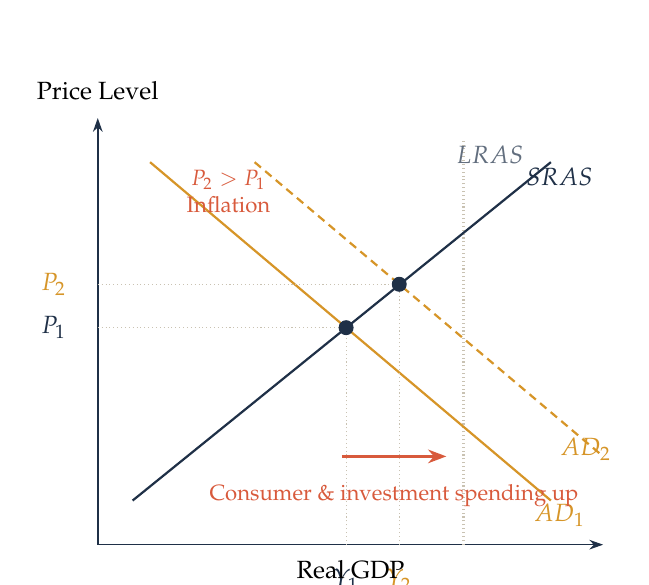
\begin{tikzpicture}[scale=1.0, baseline=(current bounding box.center)]
  \begin{axis}[econ chart,
    xlabel style={at={(ticklabel cs:0.5)}, anchor=north}, width=8cm, height=7cm, xmin=0, xmax=5.8, ymin=0, ymax=5.8,
    xlabel={\small Real GDP},
    ylabel={\small Price Level},
    xtick=\empty, ytick=\empty]
    % LRAS (vertical)
    \addplot[guide line, very thick] coordinates {(4.2,0)(4.2,5.5)};
    \node[curve label, AxisCharcoal!70] at (4.5,5.3) {$LRAS$};

    % SRAS (original)
    \addplot[curve A, thick] coordinates {(0.4,0.6)(5.2,5.2)};
    \node[curve label, CurveNavy] at (5.3,5.0) {$SRAS$};

    % AD1 (original)
    \addplot[curve accent, thick] coordinates {(0.6,5.2)(5.2,0.6)};
    \node[curve label, CurveGold] at (5.3,0.4) {$AD_1$};

    % AD2 (shifted right)
    \addplot[curve accent shift, thick] coordinates {(1.8,5.2)(5.8,1.2)};
    \node[curve label, CurveGold] at (5.6,1.3) {$AD_2$};

    % Equilibrium 1
    % SRAS: y = 0.958x + 0.217; AD1: y = -x + 5.8 → x=2.85, y=2.95
    \addplot[econ point, mark=*] coordinates {(2.85,2.95)};
    \addplot[guide projection] coordinates {(2.85,0)(2.85,2.95)};
    \addplot[guide projection] coordinates {(0,2.95)(2.85,2.95)};
    \node[tick label, below] at (2.85,-0.2) {$Y_1$};
    \node[tick label, left] at (-0.25,2.95) {$P_1$};

    % Equilibrium 2
    % SRAS: y = 0.958x + 0.217; AD2: y = -x + 7.0 → x=3.46, y=3.54
    \addplot[econ point, mark=*] coordinates {(3.46,3.54)};
    \addplot[guide projection] coordinates {(3.46,0)(3.46,3.54)};
    \addplot[guide projection] coordinates {(0,3.54)(3.46,3.54)};
    \node[tick label, CurveGold, below] at (3.46,-0.2) {$Y_2$};
    \node[tick label, CurveGold, left] at (-0.25,3.54) {$P_2$};

    % Annotation
    \node[annot, color=CurveRose, align=center] at (1.5,4.8) {$P_2 > P_1$\\Inflation};

    % Shift arrow with cause
    \draw[-{Stealth}, CurveRose, thick] (2.8,1.2)--(4.0,1.2);
    \node[annot, CurveRose, below] at (3.4,0.95) {Consumer \& investment spending up};
  \end{axis}
\end{tikzpicture}%
}{%
\textbf{\color{NavyPrimary}Demand-Pull Inflation:}\\[4pt]
$\bullet$ AD increases (AD\textsubscript{1} $\to$ AD\textsubscript{2}) due to higher consumer or investment spending\\[2pt]
$\bullet$ Economy is at or near full employment (LRAS)\\[2pt]
$\bullet$ SRAS is upward-sloping; additional AD pushes output but raises prices\\[4pt]
\textbf{\color{NavyPrimary}Mechanism:}\\[2pt]
Real output rises (Y\textsubscript{1} $\to$ Y\textsubscript{2}) \& price level rises (P\textsubscript{1} $\to$ P\textsubscript{2})\\[4pt]
\textbf{\color{GoldAccent}Key:} Demand pulls prices up when the economy is already close to full capacity.%
}
\end{diagrambox}

\begin{diagrambox}[Cost-Push Inflation -- SRAS Shifts Left]
\diagramwithtext{%
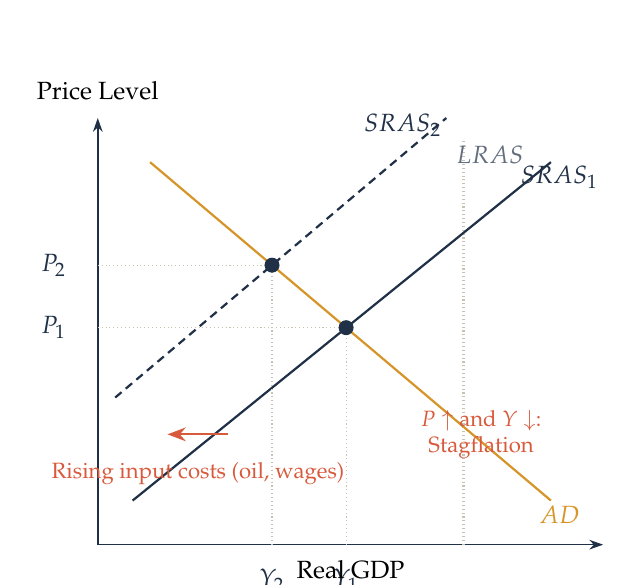
\begin{tikzpicture}[scale=1.0, baseline=(current bounding box.center)]
  \begin{axis}[econ chart,
    xlabel style={at={(ticklabel cs:0.5)}, anchor=north}, width=8cm, height=7cm, xmin=0, xmax=5.8, ymin=0, ymax=5.8,
    xlabel={\small Real GDP},
    ylabel={\small Price Level},
    xtick=\empty, ytick=\empty]
    % LRAS (vertical)
    \addplot[guide line, very thick] coordinates {(4.2,0)(4.2,5.5)};
    \node[curve label, AxisCharcoal!70] at (4.5,5.3) {$LRAS$};

    % SRAS1 (original)
    \addplot[curve primary, thick] coordinates {(0.4,0.6)(5.2,5.2)};
    \node[curve label, CurveNavy] at (5.3,5.0) {$SRAS_1$};

    % SRAS2 (shifted left/upward)
    \addplot[curve primary shift, thick] coordinates {(0.2,2.0)(4.0,5.8)};
    \node[curve label, CurveNavy] at (3.5,5.7) {$SRAS_2$};

    % AD (unchanged)
    \addplot[curve accent, thick] coordinates {(0.6,5.2)(5.2,0.6)};
    \node[curve label, CurveGold] at (5.3,0.4) {$AD$};

    % Equilibrium 1: SRAS1∩AD: 0.9583x+0.217 = -x+5.8 → x=2.85, y=2.95
    \addplot[econ point, mark=*] coordinates {(2.85,2.95)};
    \addplot[guide projection] coordinates {(2.85,0)(2.85,2.95)};
    \addplot[guide projection] coordinates {(0,2.95)(2.85,2.95)};
    \node[tick label, below] at (2.85,-0.2) {$Y_1$};
    \node[tick label, left] at (-0.25,2.95) {$P_1$};

    % Equilibrium 2
    \addplot[econ point, mark=*] coordinates {(2.0,3.8)};
    \addplot[guide projection] coordinates {(2.0,0)(2.0,3.8)};
    \addplot[guide projection] coordinates {(0,3.8)(2.0,3.8)};
    \node[tick label, below] at (2.0,-0.2) {$Y_2$};
    \node[tick label, left] at (-0.25,3.8) {$P_2$};

    % Annotation
    \node[annot, CurveRose, align=center] at (4.4,1.5) {$P \uparrow$ and $Y \downarrow$:\\Stagflation};

    % Shift arrow with cause
    \draw[-{Stealth}, CurveRose, thick] (1.5,1.5)--(0.8,1.5);
    \node[annot, CurveRose, below] at (1.15,1.25) {Rising input costs (oil, wages)};
  \end{axis}
\end{tikzpicture}%
}{%
\textbf{\color{NavyPrimary}Cost-Push Inflation:}\\[4pt]
$\bullet$ SRAS shifts left (SRAS\textsubscript{1} $\to$ SRAS\textsubscript{2}) due to rising input costs\\[2pt]
$\bullet$ Oil shocks, wage pressures, or currency depreciation increase production costs\\[2pt]
$\bullet$ AD unchanged; economy must adjust to reduced supply\\[4pt]
\textbf{\color{NavyPrimary}Result (Stagflation):}\\[2pt]
Price rises (P\textsubscript{1} $\to$ P\textsubscript{2}) but output falls (Y\textsubscript{1} $\to$ Y\textsubscript{2})\\[4pt]
\textbf{\color{GoldAccent}Key:} Supply shocks can create inflation without demand pressure.%
}
\end{diagrambox}


\begin{tcolorbox}[enhanced,colback=EvalBg,colframe=EvalFrame,arc=0pt,boxrule=1pt,title={\bfseries\color{EvalFrame}Evaluation: AD, AS, Inflation and Unemployment},fonttitle=\small]
\small\RaggedRight
\begin{itemize}[itemsep=2pt,topsep=2pt]
  \item \textbf{Demand-pull vs.\ cost-push:} The correct policy response differs. Contractionary policy works for demand-pull. For cost-push, tightening monetary policy further \textit{worsens} output (stagflation risk). \textit{``It depends on the root cause.''}
  \item \textbf{Output gap matters:} If the economy has a large negative output gap (well below LRAS), an AD increase primarily raises output with little inflation. Near full employment, the same shift is mainly inflationary.
  \item \textbf{Unemployment type determines policy:} Supply-side policies target structural unemployment; fiscal/monetary policy targets cyclical unemployment. A minimum wage can even \textit{increase} employment in a monopsony labour market.
  \item \textbf{Hysteresis:} Long-term unemployment erodes skills, raising the NRU permanently. Quick recovery of cyclical unemployment is easier than reversing structural damage.
  \item \textbf{GDP as a welfare measure:} GDP growth does not capture inequality, environmental degradation, or leisure time. HDI and GPI are broader but harder to measure.
  \item \textbf{Inflationary spiral:} Whether depreciation causes sustained inflation depends on whether unions demand compensating wage rises (a wage-price spiral), which depends on the bargaining power of labour.
\end{itemize}
\end{tcolorbox}

\subsection{Consequences of Inflation}

\begin{tcolorbox}[enhanced,colback=LightBlue,colframe=MidBlue!70,arc=0pt,boxrule=0.8pt]
\begin{tabular}{@{}>{\RaggedRight\arraybackslash}p{0.35\linewidth}>{\RaggedRight\arraybackslash}p{0.60\linewidth}@{}}
\textbf{\color{NavyPrimary}Consequence} & \textbf{\color{NavyPrimary}Explanation} \\
\midrule
\textbf{Fall in real incomes} & If wages rise slower than prices, purchasing power falls \\
\textbf{Redistribution} & Hurts savers (real value of savings falls); helps borrowers (real debt shrinks) \\
\textbf{Menu costs} & Cost of changing prices, reprinting catalogues and price tags \\
\textbf{Shoe-leather costs} & Time/effort spent minimising cash holdings that are losing value \\
\textbf{Uncertainty} & High inflation makes planning and investment difficult for firms \\
\textbf{Loss of competitiveness} & Higher inflation than trading partners $\Rightarrow$ exports become expensive \\
\midrule
\textbf{Benefit: borrowers gain} & Real value of debt falls; easier to repay \\
\textbf{Benefit: avoids deflation} & Low stable inflation prevents the deflationary spiral of falling demand and rising real debt \\
\textbf{Benefit: labour market} & Allows real wage cuts without nominal cuts, preventing unemployment \\
\end{tabular}
\end{tcolorbox}

\subsection{Exam Practice Questions -- Chapter 4}

\begin{exampractice}
\begin{enumerate}[leftmargin=*]
\item \textbf{``The UK experienced falling house prices and rising unemployment during the 2008--2009 financial crisis. Analyse how the circular flow of income explains the transition from recession to recovery during this period.''} [15 marks]
\textit{Model structure: Explain injections (I, G, X) and leakages (S, T, M). Show how falling investment and export demand reduced AD; explain how government stimulus (G) and monetary policy helped restore growth. Consider automatic stabilisers.}

\item \textbf{``Using AD/AS analysis, explain why demand-pull inflation occurred in the UK in 2021--2022, but why contractionary monetary policy alone may not solve it completely.''} [15 marks]
\textit{Model structure: Show AD shifts right while SRAS slopes upward. Explain wage-price spiral risk and cost-push effects (energy prices). Evaluate why LRAS constraints matter; supply-side policies needed for sustained recovery.}

\item \textbf{``A major oil-producing country experienced a sharp fall in oil prices, followed by deflation and rising unemployment. Use the AD/AS model to explain these outcomes and evaluate the policy options available.''} [15 marks]
\textit{Model structure: Show SRAS shift left (cost of production falls) or shifts right? Clarify: lower energy costs boost SRAS but lower export revenues reduce AD. Net effect ambiguous; depends on size of exports sector and elasticity of demand for oil.}

\item \textbf{``Distinguish between frictional, structural and cyclical unemployment. Explain why a government intent on reducing unemployment to below 3\% might face serious policy trade-offs.''} [15 marks]
\textit{Model structure: Define each type with examples. Explain NAIRU concept and the Phillips Curve trade-off. Show why supply-side policies take years; demand-side policy risks accelerating inflation if NAIRU is violated.}

\item \textbf{``Evaluate the claim that `GDP per capita is a reliable measure of a nation's living standards.' Use examples to illustrate your answer.''} [15 marks]
\textit{Model structure: Explain GDP calculation (income, expenditure, output methods). Contrast with HDI, Gini coefficient, and environmental metrics. Show UK vs. developing country comparison; highlight inequality, leisure, and sustainability issues.}
\end{enumerate}
\end{exampractice}

% ============================================================
%  CHAPTER 5: GOVERNMENT MACROECONOMIC POLICY
% ============================================================
\chapter{Government Macroeconomic Policy}

\section{Government Macroeconomic Policy Objectives}

\begin{coreidea}
Macroeconomics is the study of the whole economy. Governments actively steer it towards specific goals -- known as \textbf{macroeconomic policy objectives} -- using a toolkit of taxes, spending, and interest rates.
\end{coreidea}

Think of the government as the driver of a very large, complex bus. The passengers are businesses, consumers, and households. The driver watches three key gauges on the dashboard: the \textbf{Price Stability Gauge} (controlling inflation), the \textbf{Low Unemployment Gauge}, and the \textbf{Economic Growth Gauge}.

\subsection{Use of Government Policy to Achieve Macroeconomic Objectives}

The government uses its policy toolkit to hit three main targets. We examine each in turn.

\subsubsection{1.\ The Objective of Price Stability}

\begin{keyterm}{Price Stability}
Price stability does not mean prices never change. It means ensuring the general price level increases at a \textbf{low, stable, and predictable} rate. Governments typically target around \textbf{2\% inflation per year}.
\end{keyterm}

A little inflation is healthy; high or unpredictable inflation is dangerous. Governments pursue price stability because:

\begin{itemize}
  \item \textbf{Protects Purchasing Power:} High inflation erodes the real value of money, reducing living standards and the real value of savings.
  \item \textbf{Encourages Investment:} Businesses invest more when they are confident about future costs. High inflation creates uncertainty that deters long-term planning.
  \item \textbf{Maintains International Competitiveness:} If domestic inflation exceeds that of trading partners, exports become more expensive, harming domestic industries and widening the trade deficit.
  \item \textbf{Prevents Menu and Shoe Leather Costs:} High inflation forces firms to constantly reprice goods (\emph{menu costs}) and encourages people to avoid holding cash (\emph{shoe leather costs}).
\end{itemize}

\subsubsection{2.\ The Objective of Low Unemployment}

\begin{keyterm}{Low Unemployment}
Ensuring that as many people who are able, available, and actively seeking work can find a job. Zero unemployment is neither possible nor desirable -- some \textbf{frictional unemployment} always exists as people move between jobs.
\end{keyterm}

Governments target the \emph{lowest sustainable rate} of unemployment because:

\begin{itemize}
  \item \textbf{Maximises National Output:} Unemployed workers are unused resources, creating a negative output gap. Full employment allows the economy to produce at capacity.
  \item \textbf{Raises Living Standards:} Wages are the primary income source for most households. Employment reduces poverty and inequality.
  \item \textbf{Improves Government Finances:} More workers means more income tax and VAT revenue, and lower welfare spending -- improving the budget position.
  \item \textbf{Promotes Social Cohesion:} High long-term unemployment is linked to increased crime, poor health, and loss of skills.
\end{itemize}

\subsubsection{3.\ The Objective of Economic Growth}

\begin{keyterm}{Economic Growth}
A sustained increase in the productive capacity of an economy, measured by the annual percentage change in real GDP. \textbf{Real GDP per capita} is the best measure of improving living standards.
\end{keyterm}

\begin{itemize}
  \item \textbf{Raises Average Living Standards:} More output per person means people can consume more and enjoy better public services.
  \item \textbf{Creates Jobs:} Higher output requires more workers, driving down unemployment.
  \item \textbf{Increases Tax Revenues:} A larger economy automatically generates more tax revenue, funding schools, hospitals, and infrastructure.
  \item \textbf{Helps Reduce Poverty:} Growth creates opportunities for more people to enter work and increase their incomes.
\end{itemize}

% ─────────────────────────────────────────────────────────────
\section{Fiscal Policy}

\begin{keyterm}{Fiscal Policy}
The use of \textbf{government spending (G)} and \textbf{taxation (T)} to influence the level of Aggregate Demand (AD) and the overall economy. It is the government's primary tool for managing the economic cycle.
\end{keyterm}

\subsection{Meaning of the Government Budget}

The government budget is an annual financial statement presenting planned tax revenues and planned expenditures for the coming year.

\begin{itemize}
  \item \textbf{Taxation (T):} The government's main revenue source -- income tax, corporation tax, VAT, and excise duties on fuel, alcohol, and tobacco.
  \item \textbf{Government Spending (G):} All state expenditure -- public sector wages (teachers, nurses), infrastructure projects, welfare payments, and defence.
\end{itemize}

The budget also signals the government's \emph{fiscal stance}: a plan to raise spending or cut taxes signals \textbf{expansionary} policy; cutting spending or raising taxes signals \textbf{contractionary} policy.

\subsection{Budget Deficit and Budget Surplus}

\begin{keyterm}{Budget Deficit}
Occurs when government expenditure (G) exceeds tax revenue (T) in a given year: $G > T$. The government must \textbf{borrow} to cover the shortfall, adding to the national debt. Common during recessions.
\end{keyterm}

\begin{keyterm}{Budget Surplus}
Occurs when tax revenue (T) exceeds government expenditure (G): $T > G$. The surplus can be used to repay existing national debt. Surpluses are less common and typically occur during periods of strong growth.
\end{keyterm}

\subsection{Meaning and Significance of National Debt}

\begin{keyterm}{National Debt}
The \textbf{total stock} of outstanding government borrowings accumulated over time -- the sum of all past budget deficits, minus any surpluses. It is a \textbf{stock} concept (measured at a point in time), whereas the annual budget deficit is a \textbf{flow} concept.
\end{keyterm}

National debt is expressed as a \textbf{percentage of GDP} to allow meaningful comparison across time and between countries (a \pounds2 trillion debt means very different things to the USA and to Greece).

\begin{example}[Significance of National Debt]
\textbf{Negative effects:} High debt leads to large interest payments that crowd out spending on public services. Loss of investor confidence may force the government to offer higher interest rates, worsening the problem. In extreme cases it triggers a sovereign debt crisis.\\[4pt]
\textbf{Positive effects:} If debt finances productive investment (infrastructure, education, R\&D), it raises the economy's long-run productive capacity, making future debt repayment easier.
\end{example}

\subsection{Taxation}

\subsubsection{Types of Taxes}

\begin{itemize}
  \item \textbf{Direct Taxes:} Levied on income or wealth. Examples: Income Tax, Corporation Tax, National Insurance, Inheritance Tax. Tend to be progressive and harder to avoid.
  \item \textbf{Indirect Taxes:} Levied on goods and services, paid by consumers via sellers. Examples: VAT, Excise Duties. Tend to be regressive; can be avoided by not buying the taxed good.
\end{itemize}

\subsubsection{Tax Structures}

\begin{itemize}
  \item \textbf{Progressive Tax:} Average tax rate \emph{rises} with income (e.g.\ UK Income Tax brackets: 0\%, 20\%, 40\%, 45\%). Reduces income inequality.
  \item \textbf{Regressive Tax:} Average tax rate \emph{falls} as income rises (e.g.\ a fixed-rate VAT takes a larger share of a low earner's income). The burden falls disproportionately on the poor.
  \item \textbf{Proportional Tax:} Average tax rate remains \emph{constant} regardless of income (e.g.\ a flat tax of 20\%).
\end{itemize}

\subsubsection{Marginal and Average Rates of Taxation}

\begin{keyterm}{Marginal Rate of Tax (MRT)}
The rate of tax paid on the \textbf{next pound earned}. If the next \pounds1{,}000 is taxed at 40\%, the MRT is 40\%.
\end{keyterm}

\begin{keyterm}{Average Rate of Tax (ART)}
Total tax paid divided by total income. If you earn \pounds50{,}000 and pay \pounds10{,}000 in tax, your ART is 20\%.
\end{keyterm}

\subsubsection{Reasons for Taxation}

\begin{itemize}
  \item To finance government spending on public services.
  \item To redistribute income and reduce inequality.
  \item To manage Aggregate Demand as a fiscal policy tool.
  \item To correct market failures -- ``sin taxes'' on demerit goods (e.g.\ tobacco, alcohol) internalise negative externalities.
\end{itemize}

\subsection{Government Spending}

\subsubsection{Types of Government Spending}

\begin{itemize}
  \item \textbf{Capital (Investment) Spending:} Spending on long-term assets -- new schools, hospitals, roads, railways. Increases productive potential.
  \item \textbf{Current Spending:} Day-to-day running costs -- wages for teachers, nurses and police; welfare benefits (pensions, unemployment pay); interest payments on national debt.
\end{itemize}

\subsubsection{Reasons for Government Spending}

\begin{itemize}
  \item To provide \textbf{public goods} (non-rival, non-excludable) that the free market would under-provide.
  \item To provide \textbf{merit goods} with positive externalities that would be under-consumed if left to the market.
  \item To \textbf{redistribute income} through welfare payments and state pensions.
  \item To \textbf{stabilise the economy} by smoothing the economic cycle.
\end{itemize}

\subsection{Expansionary vs.\ Contractionary Fiscal Policy}

\begin{keyterm}{Expansionary Fiscal Policy}
Increasing G and/or decreasing T. Used during a \textbf{recession} to boost AD, raise output, and reduce unemployment. Shifts the AD curve \textbf{rightward}.
\end{keyterm}

\begin{keyterm}{Contractionary Fiscal Policy}
Decreasing G and/or increasing T. Used during a \textbf{boom} to reduce AD and control inflation. Shifts the AD curve \textbf{leftward}.
\end{keyterm}

\subsubsection{Automatic Stabilisers}

\begin{keyterm}{Automatic Stabilisers}
Features of the tax and welfare system that automatically stabilise the economy \emph{without} new government action. In a boom: rising incomes generate more tax and fewer welfare payments, cooling the economy. In a recession: falling incomes generate less tax and more welfare payments, supporting AD.
\end{keyterm}

Examples: progressive income tax and unemployment benefits.

\subsection{AD/AS Analysis of Fiscal Policy}

\subsubsection{Expansionary Fiscal Policy}

\begin{diagrambox}[AD/AS: Expansionary Fiscal Policy]
\diagramwithtext{%
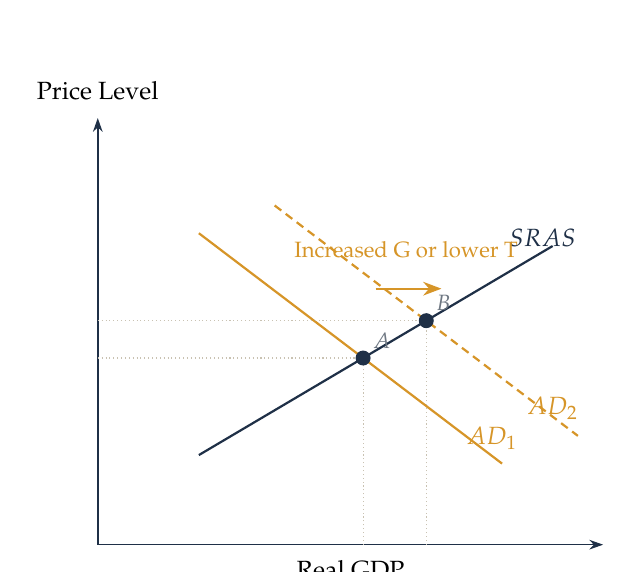
\begin{tikzpicture}[scale=1.0, baseline=(current bounding box.center)]
  \begin{axis}[econ chart, width=8.0cm, height=7.0cm, xmin=0, xmax=100, ymin=0, ymax=100,
    xlabel style={at={(ticklabel cs:0.5)}, anchor=north},
    xlabel={\small Real GDP},
    ylabel={\small Price Level},
    xtick=\empty, ytick=\empty]
    % SRAS
    \addplot[curve primary, thick, domain=20:90] {0.7*x+7};
    \node[curve label, CurveNavy] at (88,72) {$SRAS$};

    % AD1 (original)
    \addplot[curve accent, thick, domain=20:80] {-0.9*x+91};
    \node[curve label, CurveGold] at (78,25) {$AD_1$};

    % AD2 (shifted right)
    \addplot[curve accent shift, thick, domain=35:95] {-0.9*x+111};
    \node[curve label, CurveGold] at (90,32) {$AD_2$};

    % Equilibrium projections
    \addplot[guide projection] coordinates {(52.5,0)(52.5,43.75)};
    \addplot[guide projection] coordinates {(0,43.75)(52.5,43.75)};
    \addplot[guide projection] coordinates {(65,0)(65,52.5)};
    \addplot[guide projection] coordinates {(0,52.5)(65,52.5)};

    % Equilibrium markers
    \addplot[econ point, mark=*] coordinates {(52.5,43.75)(65,52.5)};
    \node[annot, above right] at (52.5,43.75) {$A$};
    \node[annot, above right] at (65,52.5) {$B$};

    % Arrow with cause label
    \draw[-{Stealth}, CurveGold, thick] (55,60) -- (68,60);
    \node[annot, CurveGold, above] at (61,65) {Increased G or lower T};
  \end{axis}
\end{tikzpicture}%
}{%
\textbf{\color{NavyPrimary}Mechanism:}\\[4pt]
Government increases G or decreases T $\Rightarrow$ Consumption and Investment rise\\[2pt]
$\bullet$ AD shifts right (AD\textsubscript{1} $\to$ AD\textsubscript{2})\\[4pt]
\textbf{\color{NavyPrimary}Outcomes:}\\[2pt]
$\bullet$ Real Output: rises (Y\textsubscript{1} $\to$ Y\textsubscript{2})\\[2pt]
$\bullet$ Price Level: rises (P\textsubscript{1} $\to$ P\textsubscript{2})\\[2pt]
$\bullet$ Employment: increases as firms hire more workers\\[4pt]
\textbf{\color{GoldAccent}Key:} Expansionary fiscal policy directly boosts AD through government demand.%
}
\end{diagrambox}

\subsubsection{Contractionary Fiscal Policy}

\textbf{Action:} Government decreases G or increases T $\Rightarrow$ C and I fall $\Rightarrow$ AD shifts left.

\begin{itemize}
  \item Real Output: falls
  \item Price Level: falls (inflation controlled)
  \item Employment: decreases as firms cut back production
\end{itemize}

\begin{coreidea}
The impact on output vs.\ prices depends on the shape of the AS curve. With \textbf{spare capacity} (flat AS), expansionary policy mainly raises output with little inflation. Near \textbf{full capacity} (steep AS), it mainly causes inflation with little extra output.
\end{coreidea}

\begin{evaluation}{Aggregate Demand and Its Components}
\textbf{Strengths / Arguments For:}
\begin{itemize}[leftmargin=*, nosep]
\item The AD/AS framework provides a clear mechanism linking policy tools (G, T, interest rates) to macroeconomic outcomes.
\item Helps identify whether an economic problem is demand-side or supply-side, guiding appropriate policy response.
\item Captures the export competitiveness effect of exchange rate changes and inflation differentials.
\end{itemize}
\textbf{Limitations / Arguments Against:}
\begin{itemize}[leftmargin=*, nosep]
\item The AD curve is a simplification; it assumes a single price level, but in reality different goods face different prices.
\item The downward slope relies on assumptions (real balance effect, interest rate effect) that may not hold in deep recessions or high-inflation environments.
\item Assumes the components of AD (C, I, G, X-M) can be treated independently, but in reality they are interdependent.
\end{itemize}
\textbf{It depends on\ldots}
\begin{itemize}[leftmargin=*, nosep]
\item The state of the economy; AD shocks matter more in shallow recessions, less near full employment.
\item Monetary transmission; whether central banks can actually influence spending via interest rates (liquidity trap).
\item International linkages; in a highly open economy, the trade component (X-M) is volatile and sensitive to exchange rates.
\end{itemize}
\end{evaluation}

% ─────────────────────────────────────────────────────────────
\section{Monetary Policy}

\subsection{Definition of Monetary Policy}

\begin{keyterm}{Monetary Policy}
The set of official policies taken by the \textbf{central bank} (e.g.\ Bank of England, Federal Reserve) to manage the \textbf{price} and \textbf{quantity of money} in the economy to achieve key macroeconomic objectives.
\end{keyterm}

\begin{itemize}
  \item \textbf{Price of Money} = the \textbf{interest rate}. By setting the base rate, the central bank influences the cost of borrowing and the reward to saving for all households and firms.
  \item \textbf{Quantity of Money} = the total stock of money (cash + bank deposits) circulating in the economy. Controlling this influences how much is available for spending and investment.
\end{itemize}

\subsection{Tools of Monetary Policy}

\subsubsection{1.\ Interest Rates}

The most commonly used modern tool. The central bank sets the \textbf{base interest rate} (policy rate) -- the rate at which it lends to commercial banks. Commercial banks then set their own rates for mortgages, loans, and savings.

\begin{itemize}
  \item \textbf{To reduce spending:} Raise the base rate $\Rightarrow$ commercial banks raise lending rates $\Rightarrow$ borrowing expensive, saving attractive $\Rightarrow$ C and I fall $\Rightarrow$ AD falls.
  \item \textbf{To increase spending:} Lower the base rate $\Rightarrow$ borrowing cheap, saving less rewarding $\Rightarrow$ C and I rise $\Rightarrow$ AD rises.
\end{itemize}

\subsubsection{2.\ Money Supply (Open Market Operations)}

\begin{itemize}
  \item \textbf{To reduce money supply:} The central bank \emph{sells} government bonds to commercial banks. Banks pay with reserves, taking money out of circulation (\textbf{contractionary}).
  \item \textbf{To increase money supply:} The central bank \emph{buys} government bonds from commercial banks, crediting their reserves -- injecting new money (\textbf{expansionary}). At the extreme this is \textbf{Quantitative Easing (QE)}.
\end{itemize}

\subsubsection{3.\ Credit Regulations}

\begin{itemize}
  \item \textbf{Reserve Requirements:} Commercial banks must hold a minimum percentage of deposits as reserves. A higher requirement restricts lending; a lower one expands it.
  \item \textbf{Direct Controls \& Moral Suasion:} The central bank can impose limits on specific lending (e.g.\ mortgages) or informally persuade banks to lend more or less.
\end{itemize}

\subsection{Expansionary vs.\ Contractionary Monetary Policy}

\begin{keyterm}{Expansionary (Loose) Monetary Policy}
Aims to \textbf{boost AD} and stimulate growth -- used during a recession or when unemployment is high. Actions: lower interest rates; increase money supply (e.g.\ QE); lower reserve requirements.
\end{keyterm}

\begin{keyterm}{Contractionary (Tight) Monetary Policy}
Aims to \textbf{reduce AD} and control inflation -- used during a boom. Actions: raise interest rates; decrease money supply; raise reserve requirements.
\end{keyterm}

\subsection{AD/AS Analysis of Monetary Policy}

\subsubsection{Expansionary Monetary Policy}

\begin{diagrambox}[AD/AS: Expansionary Monetary Policy]
\diagramwithtext{%
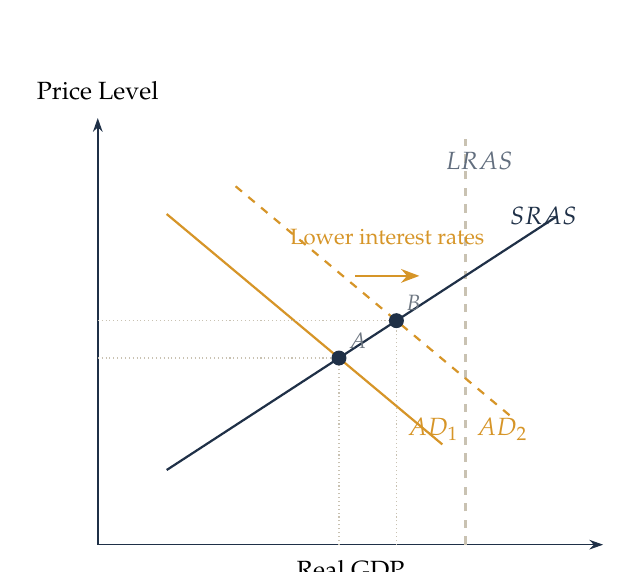
\begin{tikzpicture}[scale=1.0, baseline=(current bounding box.center)]
  \begin{axis}[econ chart, width=8.0cm, height=7.0cm, xmin=0, xmax=110, ymin=0, ymax=100,
    xlabel style={at={(ticklabel cs:0.5)}, anchor=north},
    xlabel={\small Real GDP},
    ylabel={\small Price Level},
    xtick=\empty, ytick=\empty]
    % LRAS
    \addplot[guide line, very thick, dashed, domain=0:95] coordinates {(80,0)(80,95)};
    \node[curve label, AxisCharcoal!70] at (83,90) {$LRAS$};

    % SRAS
    \addplot[curve primary, thick, domain=15:100] {0.7*x+7};
    \node[curve label, CurveNavy] at (97,77) {$SRAS$};

    % AD1 (original)
    \addplot[curve accent, thick, domain=15:75] {-0.9*x+91};
    \node[curve label, CurveGold] at (73,27) {$AD_1$};

    % AD2 (shifted right)
    \addplot[curve accent shift, thick, dashed, domain=30:90] {-0.9*x+111};
    \node[curve label, CurveGold] at (88,27) {$AD_2$};

    % Equilibrium projections
    \addplot[guide projection] coordinates {(52.5,0)(52.5,43.75)};
    \addplot[guide projection] coordinates {(0,43.75)(52.5,43.75)};
    \addplot[guide projection] coordinates {(65,0)(65,52.5)};
    \addplot[guide projection] coordinates {(0,52.5)(65,52.5)};

    % Equilibrium markers
    \addplot[econ point, mark=*] coordinates {(52.5,43.75)(65,52.5)};
    \node[annot, above right] at (52.5,43.75) {$A$};
    \node[annot, above right] at (65,52.5) {$B$};

    % Arrow with cause label
    \draw[-{Stealth}, CurveGold, thick] (56,63) -- (70,63);
    \node[annot, CurveGold, above] at (63,68) {Lower interest rates};
  \end{axis}
\end{tikzpicture}%
}{%
\textbf{\color{NavyPrimary}Mechanism:}\\[4pt]
Central bank lowers interest rates $\Rightarrow$ Consumption and Investment rise\\[2pt]
$\bullet$ AD shifts right (A $\to$ B)\\[4pt]
\textbf{\color{NavyPrimary}Outcomes:}\\[2pt]
$\bullet$ Real Output: rises toward full employment (Y\textsubscript{1} $\to$ Y\textsubscript{fe})\\[2pt]
$\bullet$ Price Level: rises (P\textsubscript{1} $\to$ P\textsubscript{2})\\[2pt]
$\bullet$ Employment: increases as firms hire more workers\\[4pt]
\textbf{\color{GoldAccent}Key:} Lower borrowing costs stimulate C and I, shifting AD right.%
}
\end{diagrambox}

\subsubsection{Contractionary Monetary Policy}

\textbf{Action:} Central bank raises interest rates $\Rightarrow$ C and I fall $\Rightarrow$ AD shifts left.

\begin{itemize}
  \item Real Output: decreases (can cause recession)
  \item Price Level: falls (inflation controlled)
  \item Employment: decreases as firms cut back production
\end{itemize}

\begin{evaluation}{Monetary Policy Transmission and Effectiveness}
\textbf{Strengths:}
\begin{itemize}[leftmargin=*, nosep]
\item Flexible and responsive; central banks can adjust rates quickly without parliamentary approval.
\item Works through multiple channels: interest rate effect on C \& I, exchange rate effect on net exports, asset price effects on wealth.
\item Credible monetary policy anchors inflation expectations, making policy more effective.
\end{itemize}
\textbf{Limitations:}
\begin{itemize}[leftmargin=*, nosep]
\item Liquidity trap: when interest rates are near zero, further cuts cannot stimulate spending; money is not a constraint, but confidence is.
\item Variable lags; transmission through the financial system and expectations is uncertain and can take 12--18 months.
\item Cannot stimulate supply-side growth; monetary policy only affects demand.
\item May cause unintended asset bubbles (low rates inflate house and stock prices) and financial stability risks.
\end{itemize}
\textbf{It depends on\ldots}
\begin{itemize}[leftmargin=*, nosep]
\item The interest rate level; policy is effective when rates are positive but becomes impotent near zero.
\item Bank lending; QE only works if banks pass on cheap funding to firms and households (credit channel); in deep recessions, banks hoard capital.
\item Exchange rate sensitivity; depreciation from lower rates boosts exports but may cause import price inflation (cost-push).
\end{itemize}
\end{evaluation}

% ─────────────────────────────────────────────────────────────
\section{Supply-Side Policy}

\subsection{Meaning of Supply-Side Policy and Effect on LRAS}

\begin{keyterm}{Supply-Side Policy}
Government measures designed to \textbf{increase the productive potential} of the economy by making markets work more efficiently and incentivising firms to produce more. Supply-side policies shift the \textbf{LRAS curve to the right}.
\end{keyterm}

\begin{coreidea}
The LRAS curve represents the maximum output an economy can produce with all resources fully and efficiently employed (the full employment level). A rightward shift means the economy can produce more real output at every price level. The core purpose is \textbf{long-term economic growth without causing inflation}.
\end{coreidea}

\subsection{Objectives of Supply-Side Policy}

\begin{itemize}
  \item \textbf{Increasing Productivity:} Output per worker (or per hour). Higher productivity lowers average costs for firms, making the economy more efficient.
  \item \textbf{Increasing Productive Capacity:} Expanding the maximum possible output of the economy to sustain higher living standards and a growing population.
  \item \textbf{Improving Competitiveness:} Higher productivity and lower costs make exports cheaper and higher quality for foreign buyers, boosting the balance of trade and attracting foreign investment.
\end{itemize}

\subsection{Tools of Supply-Side Policy}

\subsubsection{Education and Training}

Investment in schools, universities, and vocational training (e.g.\ apprenticeships) creates a more skilled, productive, and adaptable workforce. Skilled workers can use advanced technology, directly shifting LRAS rightward.

\subsubsection{Infrastructure Development}

Government spending on transport (roads, railways, ports), broadband, and energy reduces business costs and attracts foreign investment, increasing the efficiency and productive capacity of the whole economy.

\subsubsection{Support for Technological Improvement}

Grants, tax credits, or subsidies for R\&D, and direct government funding of scientific research, drive innovation and more efficient production processes -- a key driver of long-run growth.

\subsubsection{Other Measures}

\begin{itemize}
  \item \textbf{Taxation Reforms:} Lower income taxes increase the incentive to work; lower corporation tax encourages investment and attracts multinationals.
  \item \textbf{Labour Market Reforms:} Making markets more flexible (e.g.\ reducing trade union power, easier hiring and firing) reduces unemployment and improves responsiveness.
  \item \textbf{Privatisation:} Selling state-owned assets to the private sector. Theory: private firms are more efficient and profit-driven, leading to better services and lower prices.
  \item \textbf{Deregulation:} Removing unnecessary regulations lowers costs and encourages new firms, increasing competition and efficiency.
  \item \textbf{Immigration Policy:} Relaxing immigration for skilled workers quickly increases the size and quality of the labour force, filling skill shortages.
\end{itemize}

\subsection{AD/AS Analysis of Supply-Side Policy}

\begin{diagrambox}[AD/AS: Supply-Side Policy]
\diagramwithtext{%
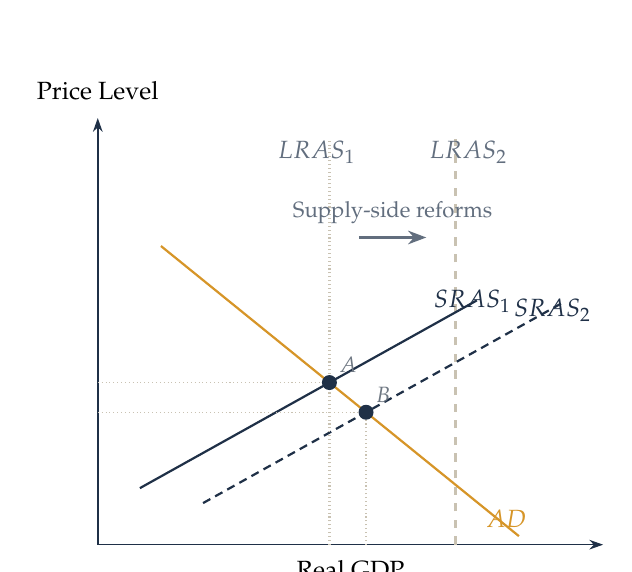
\begin{tikzpicture}[scale=1.0, baseline=(current bounding box.center)]
  \begin{axis}[econ chart, width=8.0cm, height=7.0cm, xmin=0, xmax=120, ymin=0, ymax=100,
    xlabel style={at={(ticklabel cs:0.5)}, anchor=north},
    xlabel={\small Real GDP},
    ylabel={\small Price Level},
    xtick=\empty, ytick=\empty]
    % LRAS1 (original)
    \addplot[guide line, very thick, domain=0:95] coordinates {(55,0)(55,95)};
    \node[curve label, AxisCharcoal!70] at (52,92) {$LRAS_1$};

    % LRAS2 (shifted right)
    \addplot[guide line, very thick, dashed, domain=0:95] coordinates {(85,0)(85,95)};
    \node[curve label, AxisCharcoal!70] at (88,92) {$LRAS_2$};

    % SRAS1 (original) -- intercept 7.75 so SRAS1(55)=38.0=AD(55) exactly
    \addplot[curve primary, thick, domain=10:90] {0.55*x+7.75};
    \node[curve label, CurveNavy] at (89,57) {$SRAS_1$};

    % SRAS2 (shifted right)
    \addplot[curve primary shift, thick, domain=25:110] {0.55*x-4};
    \node[curve label, CurveNavy] at (108,55) {$SRAS_2$};

    % AD (unchanged)
    \addplot[curve accent, thick, domain=15:100] {-0.8*x+82};
    \node[curve label, CurveGold] at (97,6) {$AD$};

    % Equilibrium projections
    % A: SRAS1∩AD at x=55, y=0.55*55+7.75=38.0=−0.8*55+82=38.0 ✓
    % B: SRAS2∩AD: 0.55x−4=−0.8x+82 → 1.35x=86 → x=63.70, y=31.04 ✓
    \addplot[guide projection] coordinates {(55,0)(55,38)};
    \addplot[guide projection] coordinates {(0,38)(55,38)};
    \addplot[guide projection] coordinates {(63.7,0)(63.7,31.04)};
    \addplot[guide projection] coordinates {(0,31.04)(63.7,31.04)};

    % Equilibrium markers
    \addplot[econ point, mark=*] coordinates {(55,38)(63.7,31.04)};
    \node[annot, above right] at (55,38) {$A$};
    \node[annot, above right] at (63.7,31.04) {$B$};

    % Arrow with cause label
    \draw[-{Stealth}, AxisCharcoal!70, thick] (62,72) -- (78,72);
    \node[annot, AxisCharcoal!70, font=\footnotesize, above] at (70,73) {Supply-side reforms};
  \end{axis}
\end{tikzpicture}%
}{%
\textbf{\color{NavyPrimary}Supply-Side Policy Effect:}\\[4pt]
LRAS shifts right (LRAS\textsubscript{1} $\to$ LRAS\textsubscript{2}); SRAS also shifts right\\[2pt]
$\bullet$ Policies lower production costs (education, infrastructure, R\&D)\\[4pt]
\textbf{\color{NavyPrimary}Outcomes:}\\[2pt]
$\bullet$ Real Output: rises (Y\textsubscript{1} $\to$ Y\textsubscript{2}) -- productive capacity increases\\[2pt]
$\bullet$ Price Level: falls (P\textsubscript{1} $\to$ P\textsubscript{2}) -- more goods reduce prices\\[2pt]
$\bullet$ Employment: rises -- more output requires more workers\\[4pt]
\textbf{\color{GoldAccent}Key:} Supply-side policies increase full-employment output, enabling growth without inflation.%
}
\end{diagrambox}

\begin{coreidea}
A rightward shift in LRAS can \emph{also} stimulate AD. Higher employment raises incomes and consumption (C); lower taxes raise disposable income; higher profits boost investment (I). If AD rises alongside the supply-side improvement, the result is a much larger increase in real output -- with a more muted fall in the price level.
\end{coreidea}

\begin{tcolorbox}[enhanced,colback=EvalBg,colframe=EvalFrame,arc=0pt,boxrule=1pt,title={\bfseries\color{EvalFrame}Evaluation: Fiscal, Monetary and Supply-Side Policy},fonttitle=\small]
\small\RaggedRight
\begin{itemize}[itemsep=2pt,topsep=2pt]
  \item \textbf{Fiscal policy time lags:} Recognition lag $\to$ decision lag (parliamentary process) $\to$ implementation lag. Total: 12--24 months. By the time policy works, conditions may have changed.
  \item \textbf{Crowding out vs.\ crowding in:} Higher G financed by borrowing may raise interest rates, deterring private investment (crowding out). But if government invests in infrastructure, it may \textit{raise} private returns (crowding in). Net effect is ambiguous.
  \item \textbf{Monetary policy: liquidity trap:} At near-zero interest rates, further cuts cannot stimulate investment. QE may also fail if banks hoard reserves rather than lending.
  \item \textbf{Supply-side: time horizon:} Market-based supply-side policies (deregulation, tax cuts) take years to improve productive capacity. Education and training can take a generation. In the short run, supply-side policy does little for unemployment.
  \item \textbf{Policy conflicts:} Expansionary policy reduces unemployment but may cause inflation and a current account deficit (growth raises imports). Contractionary policy cuts inflation but risks recession. These are not simply managed with a single instrument.
  \item \textbf{Open economy constraint:} High domestic interest rates attract hot money, causing currency appreciation that damages export competitiveness -- offsetting the inflation-fighting benefit.
\end{itemize}
\end{tcolorbox}

\subsection{Exam Practice Questions -- Chapter 5}

\begin{exampractice}
\begin{enumerate}[leftmargin=*]
\item \textbf{``A recession reduced government tax revenues and increased unemployment benefit spending. Using the concept of automatic stabilisers, explain how these changes help the economy recover without new government action.''} [15 marks]
\textit{Model structure: Show circular flow with injections and withdrawals. Explain how progressive taxation and welfare create automatic cushioning; falling incomes trigger lower tax collection and higher benefit payouts, both of which support AD. Compare to discretionary fiscal policy; discuss time lags.}

\item \textbf{``Evaluate the effectiveness of monetary policy in fighting inflation during a cost-push inflation episode. Include in your answer a discussion of the role of inflation expectations.''} [15 marks]
\textit{Model structure: Show SRAS shift left. Explain that raising interest rates further depresses output (stagflation). But if central bank has credibility, expectations remain anchored and wage-price spiral is prevented. Discuss conditions for policy effectiveness; note supply-side policies needed alongside monetary tightening.}

\item \textbf{``A developing country has persistently high unemployment due to skills mismatches and outdated infrastructure. Analyse whether supply-side policies are a better tool than expansionary fiscal policy for addressing this problem.''} [15 marks]
\textit{Model structure: Show that demand-side stimulus (fiscal expansion) may raise short-run output but will not address skills gaps or infrastructure deficits. Supply-side policies (education, R\&D subsidies) raise LRAS and long-run growth. But they take years. Discuss complementary use of both policies.}

\item \textbf{``Discuss the case for government intervention in financial markets to prevent asset bubbles, even if it means accepting slightly higher inflation in the short run.''} [15 marks]
\textit{Model structure: Explain that low interest rates inflate asset prices and create instability; crashes can trigger severe recessions. But regulatory tools (macroprudential limits, capital requirements) exist. Compare to accepting bubbles and managing downturns with policy. Discuss financial stability vs. price stability trade-off.}

\item \textbf{``Compare and contrast fiscal policy and monetary policy as tools for stabilising the economy in a recession. In your answer, discuss the conditions under which one tool might be preferred over the other.''} [15 marks]
\textit{Model structure: Fiscal: direct, faces lags, politically contentious, raises debt. Monetary: flexible, may fail if at zero lower bound, affects investment via interest rates. Discuss liquidity trap (monetary ineffective), crowding out (fiscal ineffective), time horizon (both matter), and interaction effects (coordination).}
\end{enumerate}
\end{exampractice}

% ============================================================
%  CHAPTER 6: INTERNATIONAL TRADE AND EXCHANGE RATES
% ============================================================
\chapter{International Trade and Exchange Rates}

% ─────────────────────────────────────────────────────────────
\section{The Reasons for International Trade}

Nations trade for several key reasons:

\begin{itemize}
  \item \textbf{Differences in Factor Endowments:} Countries have different quantities of land, labour, capital, and entrepreneurship (the factors of production). A country with a lot of oil (like Saudi Arabia) will export it, while a country with a strong tech industry (like South Korea) will export electronics.
  \item \textbf{To Obtain Goods and Services They Cannot Produce Themselves:} This could be due to a lack of natural resources (e.g.\ Japan importing oil) or a lack of technology and expertise.
  \item \textbf{To Achieve Lower Prices and Greater Choice for Consumers:} International competition forces domestic firms to be more efficient, leading to lower prices. It also gives consumers access to a wider variety of goods (e.g.\ tropical fruits in temperate countries).
  \item \textbf{To Gain Economies of Scale:} By selling to a global market, firms can produce on a larger scale, which lowers their average cost per unit, making them more competitive.
  \item \textbf{To Improve International Relations:} Trade creates economic interdependence, which can foster stronger political and diplomatic ties between countries.
\end{itemize}

\subsection{Distinction Between Absolute and Comparative Advantage}

This is the core theory explaining why trade is beneficial, even if one country is better at producing everything.

\subsubsection{The Principle of Absolute Advantage}

\begin{keyterm}{Absolute Advantage}
A country has an absolute advantage in the production of a good if it can produce more output of that good using the same quantity of resources (or the same output using fewer resources) than another country. It's about productivity -- think: ``Who is the absolute best at making this?''
\end{keyterm}

\begin{example}[Absolute Advantage]
In one day, with the same resources:
\begin{itemize}
  \item Country A can produce 20 units of wheat OR 10 units of cloth.
  \item Country B can produce 10 units of wheat OR 20 units of cloth.
\end{itemize}
Country A has an absolute advantage in wheat. Country B has an absolute advantage in cloth. It's obvious they should trade.
\end{example}

\subsubsection{The Principle of Comparative Advantage}

\begin{keyterm}{Comparative Advantage}
A country has a comparative advantage in the production of a good if it can produce it at a \textbf{lower opportunity cost} than another country. It's about sacrifice -- think: ``What do I have to give up to make this?'' This is the more important concept. It shows that trade is beneficial even if one country is better at producing everything.
\end{keyterm}

\subsubsection{The Application of Opportunity Cost}

Opportunity cost is the next best alternative forgone when making a choice. This is the key to understanding comparative advantage.

\begin{example}[Comparative Advantage -- Step by Step]
In one day, with the same resources:
\begin{itemize}
  \item Country X can produce 20 units of wheat OR 40 units of cloth.
  \item Country Y can produce 5 units of wheat OR 15 units of cloth.
\end{itemize}

\medskip
\noindent\textbf{Step 1: Calculate Opportunity Cost}

\medskip
\begin{tabular}{@{}lll@{}}
 & \textbf{OC of 1 unit of Wheat} & \textbf{OC of 1 unit of Cloth} \\
\midrule
Country X & 2 units of Cloth & 0.5 units of Wheat \\
Country Y & 3 units of Cloth & 0.33 units of Wheat \\
\end{tabular}

\medskip
\noindent\textbf{Step 2: Identify Comparative Advantage}

Country X has a lower opportunity cost for wheat (2 cloth $<$ 3 cloth), so \textbf{Country X has a comparative advantage in wheat}. Country Y has a lower opportunity cost for cloth (0.33 wheat $<$ 0.5 wheat), so \textbf{Country Y has a comparative advantage in cloth}.

\medskip
\noindent\textbf{Step 3: The Gain from Trade}

If each country specialises in what it has a comparative advantage in and trades at an exchange rate between their opportunity costs (e.g.\ 1 wheat for 2.5 cloth), both countries end up with more of both goods than if they tried to be self-sufficient. This is the ``magic'' of comparative advantage.
\end{example}

\subsubsection{Factor Endowment}

This is the underlying reason for differences in opportunity costs. The \textbf{Heckscher-Ohlin model} states that a country will have a comparative advantage in goods that require factors of production which it has in abundance.

\begin{itemize}
  \item A \textbf{labour-abundant} country (e.g.\ Bangladesh) will have a comparative advantage in labour-intensive goods (e.g.\ textiles, garments).
  \item A \textbf{capital-abundant} country (e.g.\ Germany) will have a comparative advantage in capital-intensive goods (e.g.\ cars, machinery).
\end{itemize}

\subsection{Benefits of Specialisation and Free Trade}

\begin{keyterm}{Free Trade}
Free trade is the absence of government-imposed barriers (such as tariffs, quotas, and subsidies) to the free flow of goods and services between countries.
\end{keyterm}

\subsubsection{The Benefits of Free Trade}

\textbf{For Consumers:}
\begin{itemize}
  \item Lower prices due to increased competition and efficiency.
  \item Greater choice -- access to goods and services from around the world.
  \item Higher quality as competition encourages firms to improve.
\end{itemize}

\textbf{For Producers:}
\begin{itemize}
  \item Access to larger markets, allowing them to exploit economies of scale.
  \item Access to cheaper raw materials, lowering costs of production.
  \item Increased competition and innovation, forcing firms to be more efficient.
\end{itemize}

\textbf{For the Economy:}
\begin{itemize}
  \item More efficient allocation of resources as they shift to industries where the country has a comparative advantage.
  \item Higher GDP and economic growth.
  \item Inflow of new technology and ideas.
\end{itemize}

\subsubsection{The Trading Possibility Curve (TPC)}

This builds on the Production Possibility Curve (PPC).

\begin{itemize}
  \item The \textbf{PPC} shows the maximum combinations of two goods an economy can produce using all its resources efficiently \emph{without} trade.
  \item The \textbf{TPC} shows the combinations of two goods a country can consume after it specialises and trades.
\end{itemize}

A country specialises completely in the good where it has a comparative advantage, then trades some of that good for the other. The TPC lies \emph{outside} the original PPC (except at the point of complete specialisation). This demonstrates that with trade, a country can consume at a point that was previously unattainable, increasing its economic welfare.

\subsection{Exports, Imports and the Terms of Trade}

\begin{keyterm}{Terms of Trade (TOT)}
\[ \text{TOT Index} = \frac{\text{Index of Export Prices}}{\text{Index of Import Prices}} \times 100 \]
It measures the purchasing power of a country's exports in terms of its imports. A \textbf{rise} in the index is an improvement -- you can buy more imports for the same quantity of exports. A \textbf{fall} is a deterioration -- you have to export more to buy the same quantity of imports.
\end{keyterm}

\subsubsection{Causes of Changes in the Terms of Trade}

\textbf{An Improvement (Rise in TOT):}
\begin{itemize}
  \item Rise in Export Prices (e.g.\ due to high global demand for your commodities like oil).
  \item Fall in Import Prices (e.g.\ due to technological improvements abroad making manufactured goods cheaper).
\end{itemize}

\textbf{A Deterioration (Fall in TOT):}
\begin{itemize}
  \item Fall in Export Prices (e.g.\ due to a global recession reducing demand for your goods).
  \item Rise in Import Prices (e.g.\ due to a rise in the price of essential imported raw materials).
\end{itemize}

\subsubsection{The Impact of Changes in the Terms of Trade}

\textbf{Impact of an Improvement:}
\begin{itemize}
  \item \textbf{Positive:} Higher living standards (imports are cheaper). Lower inflation (if imported raw materials are cheaper). A current account surplus is more likely.
  \item \textbf{Negative (Potential):} If export prices are too high, it might make the country's exports less competitive, reducing demand for them and potentially harming export industries and employment.
\end{itemize}

\textbf{Impact of a Deterioration:}
\begin{itemize}
  \item \textbf{Negative:} Lower living standards (imports are more expensive). Higher inflation (cost-push). A current account deficit is more likely.
  \item \textbf{Positive (Potential):} If it is due to strong domestic demand for imports, it may reflect a growing economy.
\end{itemize}

\subsection{Limitations of the Theories of Absolute and Comparative Advantage}

The theories are elegant but based on simplifying assumptions that don't always hold in the real world.

\subsubsection{The Assumptions Undermining the Theories}

\begin{itemize}
  \item \textbf{Constant Returns to Scale:} Assumes costs of production are constant. In reality, economies of scale are a major reason for trade.
  \item \textbf{No Transport Costs:} In reality, high transport costs can wipe out any comparative advantage.
  \item \textbf{Factors of Production are Immobile between Countries:} The model assumes labour and capital cannot move, but in reality there is significant international migration and capital flows.
  \item \textbf{Perfect Knowledge:} Assumes all countries have perfect information about production methods and markets.
  \item \textbf{No Trade Barriers:} Assumes free trade exists, but in reality governments use tariffs, quotas, and subsidies to protect domestic industries.
  \item \textbf{Two Countries, Two Goods:} A massive simplification of a complex global economy with over 190 countries and millions of goods.
\end{itemize}

\subsubsection{Real World Relevance}

Despite the limitations, the theories remain highly relevant because they provide a powerful logical argument for the benefits of free trade and specialisation, they explain the broad pattern of global trade, and they form the foundational intellectual basis for organisations like the \textbf{World Trade Organization (WTO)}.

However, the limitations explain why governments often do not follow pure free trade policies. They may wish to:
\begin{itemize}
  \item \textbf{Protect Infant Industries:} New industries may not be able to compete with established foreign rivals initially.
  \item \textbf{Prevent Unemployment:} A sudden shift to specialisation could cause structural unemployment in formerly protected sectors.
  \item \textbf{Ensure National Security:} Protect industries vital for defence, even if they are not internationally competitive.
  \item \textbf{Avoid Over-Specialisation:} Being over-reliant on a narrow range of exports is risky if global prices for those goods fall.
\end{itemize}

% ─────────────────────────────────────────────────────────────
\section{Protectionism}

\subsection{Meaning of Protectionism}

\begin{keyterm}{Protectionism}
Protectionism is a government's policy of shielding domestic industries and workers from foreign competition.
\end{keyterm}

It exists within international trade. While free trade is often theorised to be most efficient, governments frequently intervene to protect their own economic interests. Think of a local, fledgling football team (a domestic industry) trying to compete against a world-famous, wealthy team (foreign competition). The local council (the government) gives the local team special advantages to help them grow and survive. That's protectionism.

\subsection{Different Tools of Protection and Their Impact}

\subsubsection{1.\ Tariffs}

\textbf{What it is:} A tax imposed on imported goods.

\textbf{How it works:} It makes foreign products more expensive, so consumers are more likely to buy the cheaper domestic alternatives.

\begin{diagrambox}[Effect of a Tariff -- Price Rises, Quantity Falls]
\diagramwithtext{%
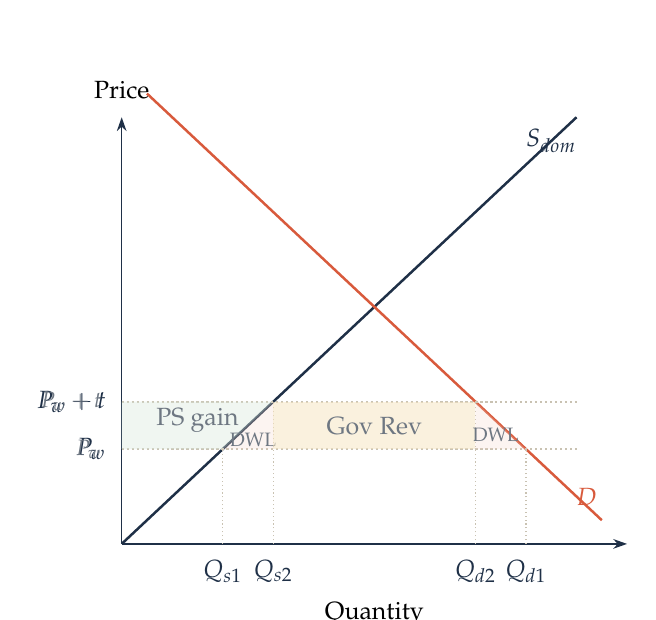
\begin{tikzpicture}[scale=1.0, baseline=(current bounding box.center)]
  \begin{axis}[
    econ chart,
    xlabel style={at={(ticklabel cs:0.5)}, anchor=north},
    width=8.0cm, height=7.0cm,
    xmin=0, xmax=100, ymin=0, ymax=90,
    xlabel={\small Quantity},
    ylabel={\small Price},
    xtick={20,30,70,80},
    xticklabels={$Q_{s1}$,$Q_{s2}$,$Q_{d2}$,$Q_{d1}$},
    ytick={20,30},
    yticklabels={$P_w$,$P_w + t$},
  ]
    % Supply curve (domestic): P = Q
    \addplot[curve primary, domain=0:90] {x};
    \node[curve label, color=CurveNavy] at (axis cs:85,85) {$S_{dom}$};

    % Demand curve: P = -Q + 100
    \addplot[curve secondary, domain=5:95] {-x+100};
    \node[curve label, color=CurveRose] at (axis cs:92,10) {$D$};

    % World price (horizontal line): P_w = 20
    \addplot[guide projection, thick] coordinates {(0,20)(90,20)};
    \node[annot, AnnotGray, left] at (-2,20) {$P_w$};

    % Tariff-inclusive price (horizontal line): P_t = 30
    \addplot[guide projection, thick] coordinates {(0,30)(90,30)};
    \node[annot, AnnotGray, left] at (-2,30) {$P_w + t$};

    % Projection lines
    \addplot[guide projection] coordinates {(20,0)(20,20)};
    \addplot[guide projection] coordinates {(30,0)(30,30)};
    \addplot[guide projection] coordinates {(70,0)(70,30)};
    \addplot[guide projection] coordinates {(80,0)(80,20)};

    % Producer surplus gain: trapezoid bounded by S_dom from Q=0 to Q=30, between P=20 and S_dom
    \fill[FillPositive, opacity=0.4] (axis cs:0,20) -- (axis cs:0,30) -- (axis cs:30,30) -- (axis cs:20,20) -- cycle;
    \node[annot, AnnotGray, font=\small] at (15,26) {PS gain};

    % DWL production: triangle bounded by S_dom from Q=20 to Q=30, between P_w and S_dom
    \fill[FillNegative, opacity=0.25] (axis cs:20,20) -- (axis cs:30,30) -- (axis cs:30,20) -- cycle;
    \node[annot, AnnotGray, font=\scriptsize] at (26,22) {DWL};

    % Government revenue rectangle: (30,20) to (70,30)
    \fill[FillGold, opacity=0.55] (axis cs:30,20) -- (axis cs:70,20) -- (axis cs:70,30) -- (axis cs:30,30) -- cycle;
    \node[annot, AnnotGray, font=\small] at (50,25) {Gov Rev};

    % DWL consumption: triangle bounded by D from Q=70 to Q=80, between P_t and D
    \fill[FillNegative, opacity=0.25] (axis cs:70,30) -- (axis cs:80,20) -- (axis cs:70,20) -- cycle;
    \node[annot, AnnotGray, font=\scriptsize] at (74,23) {DWL};
  \end{axis}
\end{tikzpicture}%
}{%
\textbf{\color{NavyPrimary}Tariff Protection}\\[4pt]
$\bullet$ Tariff raises import price from P\textsubscript{w} to P\textsubscript{w}+t\\[2pt]
$\bullet$ Domestic supply rises (Q\textsubscript{s1} \(\rightarrow\) Q\textsubscript{s2}), demand falls (Q\textsubscript{d1} \(\rightarrow\) Q\textsubscript{d2})\\[2pt]
$\bullet$ Green area = producer surplus gain\\[2pt]
$\bullet$ Gold rectangle = government revenue\\[2pt]
$\bullet$ Red triangles = deadweight welfare loss (production + consumption inefficiency)\\[2pt]
\textbf{\color{GoldAccent}Key:} Tariff protects domestic producers but reduces allocative efficiency%
}
\end{diagrambox}

\textbf{Impact:}
\begin{itemize}
  \item \textbf{On Price \& Quantity:} The supply curve for the imported good shifts leftwards, leading to a higher price ($P_w$ to $P_t$) and lower quantity of imports.
  \item \textbf{On Domestic Producers:} They are protected -- they can sell more at a higher price because their goods are relatively cheaper than the taxed imports.
  \item \textbf{On Consumers:} They lose out -- they face higher prices and have less choice.
  \item \textbf{On Government:} They gain revenue equal to the tariff amount $\times$ the quantity of imports after the tariff.
  \item \textbf{On Efficiency:} It can lead to a loss of allocative efficiency as resources are diverted to less efficient domestic producers (the domestic welfare loss, shown by triangles on a diagram).
\end{itemize}

\subsubsection{2.\ Import Quotas}

\textbf{What it is:} A physical limit on the quantity of a good that can be imported over a period.

\textbf{How it works:} It directly restricts the volume of foreign goods entering the country, creating an artificial scarcity.

\textbf{Impact:}
\begin{itemize}
  \item \textbf{On Price \& Quantity:} The supply of imports is fixed at the quota level. This scarcity drives up the price. The effect on price is similar to a tariff.
  \item \textbf{On Domestic Producers:} Protected, just like with a tariff.
  \item \textbf{On Consumers:} Same negative impact as tariffs: higher prices, less choice.
  \item \textbf{On Government:} No direct revenue (unless they sell the import licences). The extra profit from the higher price (the ``quota rent'') often goes to the foreign producers who managed to get a licence to import.
\end{itemize}

\textbf{Key Difference from Tariff:} A quota is a physical limit, while a tariff is a tax. Quotas can be more restrictive and less transparent.

\subsubsection{3.\ Export Subsidies}

\textbf{What it is:} A payment from the government to domestic firms to encourage exports.

\textbf{How it works:} It lowers the production costs for domestic firms, allowing them to sell their goods abroad at a more competitive price (or even below cost).

\textbf{Impact:}
\begin{itemize}
  \item \textbf{On Domestic Firms:} They can compete more easily in international markets. Their production increases.
  \item \textbf{On Foreign Producers:} They are hurt because they face unfair, subsidised competition.
  \item \textbf{On Domestic Consumers:} They can lose out because the subsidised goods are diverted away from the domestic market, potentially leading to higher prices at home.
  \item \textbf{On Government:} It is a cost to the treasury (funded by taxpayers) and can lead to disputes at the WTO.
\end{itemize}

\subsubsection{4.\ Embargoes}

\textbf{What it is:} A complete ban on trade with a specific country, or on a specific type of product.

\textbf{How it works:} The most extreme form of protectionism, often used for political rather than purely economic reasons (e.g.\ sanctions).

\textbf{Impact:}
\begin{itemize}
  \item Total elimination of the targeted imports or exports.
  \item Severe disruption for both the imposing country and the target country.
  \item Domestic producers are completely shielded from that particular foreign competitor.
  \item Consumers lose access to those goods entirely.
\end{itemize}

\subsubsection{5.\ Excessive Administrative Burdens (`Red Tape')}

\textbf{What it is:} Creating complex, time-consuming, and costly customs procedures, health standards, safety regulations, or labelling requirements.

\textbf{How it works:} It doesn't ban imports, but it makes the process so difficult and expensive that it discourages foreign firms from even trying to sell in the market.

\textbf{Impact:}
\begin{itemize}
  \item Increases the time and cost of importing.
  \item Acts as a hidden barrier to trade, often disguised as a measure to protect consumers or the environment.
  \item Can be very effective at reducing imports without an official tariff or quota.
\end{itemize}

\subsection{Arguments For and Against Protection}

\subsubsection{Arguments FOR Protection}

\begin{itemize}
  \item \textbf{Infant Industry Argument:} New, fledgling domestic industries (``infants'') cannot compete with large, established foreign rivals. They need temporary protection (e.g.\ tariffs) to grow, achieve economies of scale, and become efficient. \emph{Example: protecting a new solar panel industry from established Chinese manufacturers.} Problem: It's hard to remove protection later, and it's difficult to pick which industries will eventually succeed.

  \item \textbf{Sunset Industries:} The opposite of infant industries. Declining, old industries (e.g.\ traditional steel) are protected to prevent sudden, large-scale unemployment and allow for a managed, slower decline and retraining of workers.

  \item \textbf{Strategic Industries:} Certain industries are vital for national security and should not be reliant on other countries. Examples: defence, energy, and food production.

  \item \textbf{Preventing Dumping:} Dumping is when a country sells goods in another country at a price below their cost of production, to drive domestic competitors out of business. Protectionism (anti-dumping tariffs) is a legitimate defence against this ``unfair'' trade.

  \item \textbf{Improving the Balance of Trade:} By restricting imports, a country can reduce its trade deficit. This can protect foreign exchange reserves.

  \item \textbf{Improving Terms of Trade:} A large country can use a tariff to force down the world price of the good it is importing. This means it gives up fewer exports to pay for its imports, improving its terms of trade.
\end{itemize}

\subsubsection{Arguments AGAINST Protection}

\begin{itemize}
  \item \textbf{Anti-Specialisation:} Protectionism discourages countries from specialising in what they are best at producing (their comparative advantage). This leads to a misallocation of resources globally, making the world as a whole poorer.

  \item \textbf{Increased Prices for Consumers:} As seen with tariffs and quotas, protectionism invariably leads to higher prices, reducing consumers' real income and living standards.

  \item \textbf{Lower Quality and Less Choice:} Shielded from international competition, domestic firms have less incentive to innovate, improve efficiency, or increase the quality of their products.

  \item \textbf{Trade Wars:} If one country erects trade barriers, its trading partners are likely to retaliate with their own barriers. The result is a spiral of restrictions that reduces world trade, harms global economic growth, and leaves everyone worse off. Everyone loses the gains from trade.
\end{itemize}

\textbf{Weighing the Arguments:} The strength of the case for or against protection depends heavily on context. The infant industry argument is theoretically sound but historically prone to government failure -- industries rarely ``graduate'' from protection as intended, and picking winners is notoriously difficult. Protection to correct dumping may be justified, but governments frequently misuse anti-dumping rules to shield inefficient domestic producers. The terms of trade argument only works for large countries with genuine market power over world prices; for small open economies, it is irrelevant. Short-run protection to ease structural adjustment (sunset industries) can be justified on equity grounds, but only if accompanied by active retraining policies -- otherwise it merely delays inevitable decline at consumers' expense. Finally, the national security argument is compelling for genuinely strategic goods but is often stretched to cover industries with no real defence significance. In practice, economists generally find that the long-run costs of protection outweigh the short-run gains, particularly when retaliation and dynamic efficiency losses are considered.

\begin{evaluation}{Free Trade vs. Protectionism}
\textbf{Strengths / Arguments For Free Trade:}
\begin{itemize}[leftmargin=*, nosep]
\item Comparative advantage theory shows gains from specialisation for all trading partners.
\item Increases consumer choice and lowers prices due to competition.
\item Encourages innovation and efficiency; firms cannot hide behind trade barriers.
\item Avoids costly retaliatory trade wars that harm all sides.
\end{itemize}
\textbf{Strengths / Arguments For Protectionism:}
\begin{itemize}[leftmargin=*, nosep]
\item Protects infant industries until they achieve scale economies (temporary protection justified).
\item Allows orderly adjustment for sunset industries; prevents mass unemployment.
\item Maintains domestic capacity in strategic industries vital for national security or food security.
\item Can improve terms of trade for large countries with market power.
\end{itemize}
\textbf{Limitations and Caveats:}
\begin{itemize}[leftmargin=*, nosep]
\item Protection is hard to remove once granted; politically created, politically entrenched.
\item Deadweight loss from protection is typically larger than the gains to protected producers.
\item Retaliatory trade wars can reverse all gains from trade and reduce global growth.
\item Protectionism may signal weakness, leading to investment flight and currency depreciation.
\end{itemize}
\textbf{It depends on\ldots}
\begin{itemize}[leftmargin=*, nosep]
\item The maturity of the industry; genuinely infant industries can grow into competitive ones.
\item The country's market size; small economies benefit much more from trade than large protectionist ones.
\item The presence of retaliation; a unilateral tariff usually invites retaliation that erases gains.
\end{itemize}
\end{evaluation}

% ─────────────────────────────────────────────────────────────
\section{Current Account of the Balance of Payments}

\subsection{The Purpose of the Balance of Payments \& Components of the Current Account}

\begin{keyterm}{Balance of Payments (BoP)}
Think of the BoP as a giant financial report card for a country. It records all financial transactions between a country's residents (including businesses) and the rest of the world over a specific period, usually a year. It is based on double-entry bookkeeping: every transaction has two sides -- a credit (+) and a debit (-) -- and in theory, the BoP should always balance to zero.
\end{keyterm}

The BoP is divided into two main accounts: the \textbf{Current Account} and the \textbf{Capital and Financial Account} (which records flows of investment and capital).

\subsubsection{The Components of the Current Account}

The current account measures the flow of income in and out of the country from trade in goods/services and other income transfers. It has four main components:

\textbf{Trade in Goods (Visible Balance)}

What it is: The export and import of physical, tangible products you can see and touch. Examples:
\begin{itemize}
  \item Credits (+): Selling cars, machinery, pharmaceuticals, and wheat to other countries.
  \item Debits (-): Buying oil, electronics, clothing, and coffee from other countries.
\end{itemize}
In the UK, this is often in a deficit (more imports than exports).

\textbf{Trade in Services (Invisible Balance)}

What it is: The export and import of intangible services. Examples:
\begin{itemize}
  \item Credits (+): A German tourist spending money in a London hotel (UK exports tourism), a UK bank providing insurance to a foreign company.
  \item Debits (-): A British student paying tuition fees to an American university (UK imports education), a UK company using a foreign shipping line.
\end{itemize}

\textbf{Primary Income}

What it is: The flow of income from factors of production (capital and labour) across borders -- money earned from investments or by working abroad. Examples:
\begin{itemize}
  \item Credits (+): Profits, dividends, and interest that UK residents receive from their investments in other countries. Wages earned by a UK citizen working temporarily in Switzerland.
  \item Debits (-): Profits, dividends, and interest paid to foreign owners of assets located in the UK (e.g.\ a Japanese car company repatriating its profits from its UK factory back to Japan).
\end{itemize}

\textbf{Secondary Income}

What it is: Transfers of money where no good, service, or asset is received in return -- essentially a one-way flow of money. Examples:
\begin{itemize}
  \item Credits (+): The UK receiving foreign aid (grants) after a natural disaster.
  \item Debits (-): The UK government sending foreign aid to developing nations, or migrants sending remittances (a portion of their earnings) back to their families in their home country.
\end{itemize}

\subsection{Calculations}

\begin{example}[Current Account Calculations (£bn)]
Assume the following for a country in one year:
\begin{itemize}
  \item Exports of Goods: 300 \quad Imports of Goods: 400
  \item Exports of Services: 150 \quad Imports of Services: 100
  \item Net Primary Income: +50 \quad Net Secondary Income: -20
\end{itemize}

\medskip
\begin{tabular}{@{}lr@{}}
\textbf{Balance} & \textbf{£bn} \\
\midrule
Trade in Goods: $300 - 400$ & $-100$ \\
Trade in Services: $150 - 100$ & $+50$ \\
\textbf{Trade in Goods \& Services} & $\mathbf{-50}$ \\
Net Primary Income & $+50$ \\
Net Secondary Income & $-20$ \\
\midrule
\textbf{Current Account Balance (CAB)} & $\mathbf{-20}$ \\
\end{tabular}

\medskip
The country has an overall current account \textbf{deficit of £20bn}.
\end{example}

\subsection{Causes of Imbalances in the Current Account}

\subsubsection{Causes of a Current Account Deficit (CAB $<$ 0)}

A deficit means the country is a net spender/borrower from the rest of the world.

\begin{itemize}
  \item \textbf{Strong Domestic Demand:} If the economy is booming, consumers have high incomes and spend more on all goods, including imports.
  \item \textbf{Lack of International Competitiveness:} High relative inflation makes goods more expensive; poor non-price competitiveness (low quality, poor design, unreliable after-sales service) compared to foreign rivals.
  \item \textbf{Strong Currency:} An overvalued exchange rate makes exports expensive for foreigners and imports cheap for domestic consumers.
  \item \textbf{Structural Factors (e.g.\ the UK):} Deindustrialisation -- a shift from manufacturing (which produces exportable goods) to services. Dependence on essential imports with low price elasticity of demand (e.g.\ oil, gas, food).
  \item \textbf{Low Productivity:} If a country's workers are less productive than those in competitor nations, it leads to higher unit costs, making exports less competitive.
\end{itemize}

\subsubsection{Causes of a Current Account Surplus (CAB $>$ 0)}

A surplus means the country is a net lender to the rest of the world.

\begin{itemize}
  \item \textbf{Strong Foreign Demand:} High economic growth in other countries increases their demand for this country's exports.
  \item \textbf{High International Competitiveness:} Low relative inflation keeps export prices competitive. A reputation for high quality and strong branding (e.g.\ German engineering, Japanese electronics) maintains demand.
  \item \textbf{Weak Currency:} An undervalued exchange rate makes exports cheap and imports expensive.
  \item \textbf{Focus on Export-Oriented Growth:} Government policies that deliberately promote exports (as seen in China and Germany historically).
  \item \textbf{Low Domestic Demand:} If an economy is in a recession, consumers cut back on spending, including on imports.
\end{itemize}

\subsection{Consequences of Imbalances}

\subsubsection{Consequences of a Current Account Deficit}

\textbf{For the Domestic Economy:}
\begin{itemize}
  \item \textbf{Lower Aggregate Demand (AD):} A deficit means spending on imports is leaking out of the circular flow, which can reduce AD and economic growth.
  \item \textbf{Deindustrialisation \& Unemployment:} If the deficit is caused by uncompetitive manufacturing, it can lead to factory closures and job losses.
  \item \textbf{Lower Standard of Living (long run):} A persistent deficit may lead to a depletion of foreign currency reserves and force a country to borrow, increasing its external debt.
\end{itemize}

\textbf{For the External Economy:}
\begin{itemize}
  \item \textbf{Depreciation of the Currency:} A deficit increases the supply of the currency on foreign exchange markets (to pay for imports), putting downward pressure on its value.
  \item \textbf{Loss of Creditor Status:} The country may become a net debtor to the rest of the world.
\end{itemize}

\subsubsection{Consequences of a Current Account Surplus}

\textbf{For the Domestic Economy:}
\begin{itemize}
  \item \textbf{Higher Aggregate Demand (AD):} A surplus means net exports (X-M) are positive, boosting AD and economic growth.
  \item \textbf{Employment in Export Industries:} Surpluses are often associated with strong export sectors, which creates jobs.
  \item \textbf{Accumulation of Foreign Assets:} The country builds up claims on the rest of the world, becoming a net creditor.
\end{itemize}

\textbf{For the External Economy:}
\begin{itemize}
  \item \textbf{Appreciation of the Currency:} High demand for the country's exports increases demand for its currency, potentially causing it to appreciate. This can eventually ``self-correct'' the surplus by making exports more expensive.
  \item \textbf{International Tensions:} Large, persistent surpluses (e.g.\ Germany, China) can be a source of trade disputes. Other countries may accuse them of unfair trade practices and retaliate with tariffs.
  \item \textbf{Imbalances Elsewhere:} One country's surplus is, by definition, another country's deficit.
\end{itemize}

% ─────────────────────────────────────────────────────────────
\section{Exchange Rates}

\subsection{Definition of Exchange Rate}

\begin{keyterm}{Exchange Rate}
An exchange rate is the price of one currency expressed in terms of another currency. It is a relative price. For example, if GBP\,1 = USD\,1.25, it means that to buy one British pound, you need to pay 1.25 US dollars. Conversely, USD\,1 = GBP\,0.80 (which is 1/1.25). These are just two ways of expressing the same relationship.
\end{keyterm}

Think of it like the price of a loaf of bread. The price tells you how many units of your currency you need to give up to get one loaf. The exchange rate tells you how many units of a foreign currency you need to give up to get one unit of your own currency (or vice versa).

\subsection{Determination of a Floating Foreign Exchange Rate}

In a \textbf{floating (or free) exchange rate} system, the value of a currency is determined by the market forces of demand and supply with no government intervention.

\textbf{Demand for Pounds (£):} People and entities need pounds to:
\begin{itemize}
  \item Buy UK exports (goods and services). A Chinese company importing British cars must pay for them in pounds.
  \item Invest in UK assets (e.g.\ stocks, bonds, property).
  \item Save money in UK banks or make speculative investments (``hot money'').
  \item Repatriate profits earned by foreign firms in the UK back to their home country.
\end{itemize}

\textbf{Supply of Pounds (£):} People and entities supply pounds (selling them to get other currencies) to:
\begin{itemize}
  \item Buy imports into the UK. A UK company importing German machinery must pay in Euros, so it sells pounds to buy Euros.
  \item Invest abroad. A UK citizen buying shares on the New York Stock Exchange sells pounds to buy US dollars.
  \item Send money abroad (e.g.\ remittances, foreign aid).
  \item Speculate that the value of the pound will fall in the future.
\end{itemize}

\begin{diagrambox}[Floating Exchange Rate: Equilibrium for GBP/USD]
\diagramwithtext{%
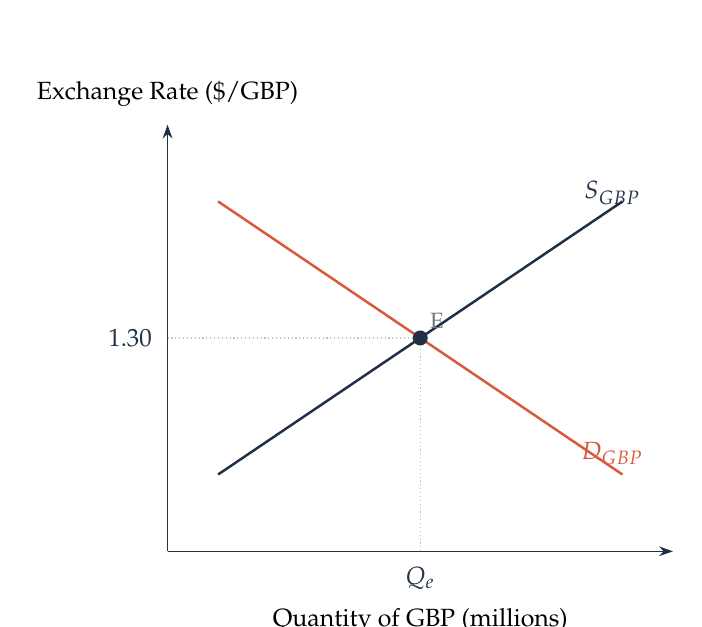
\begin{tikzpicture}[scale=1.0, baseline=(current bounding box.center)]
  \begin{axis}[
    econ chart,
    xlabel style={at={(ticklabel cs:0.5)}, anchor=north},
    width=8.0cm, height=7.0cm,
    xmin=0, xmax=100, ymin=0, ymax=100,
    xlabel={\small Quantity of GBP (millions)},
    ylabel={\small Exchange Rate (\$/GBP)},
    xtick={50}, xticklabels={$Q_e$},
    ytick={50}, yticklabels={1.30},
  ]
    % Supply of pounds curve (upward-sloping)
    \addplot[curve primary, domain=10:90] {0.8*x+10};
    \node[curve label, color=CurveNavy] at (axis cs:88,84) {$S_{GBP}$};

    % Demand for pounds curve (downward-sloping)
    \addplot[curve secondary, domain=10:90] {-0.8*x+90};
    \node[curve label, color=CurveRose] at (axis cs:88,23) {$D_{GBP}$};

    % Equilibrium projection lines
    \addplot[guide projection] coordinates {(50,0)(50,50)};
    \addplot[guide projection] coordinates {(0,50)(50,50)};

    % Equilibrium point marker
    \addplot[econ point, mark=*] coordinates {(50,50)};
    \node[annot, above right] at (50,50) {E};
  \end{axis}
\end{tikzpicture}%
}{%
\textbf{\color{NavyPrimary}Exchange Rate Equilibrium}\\[4pt]
$\bullet$ Demand for GBP from foreigners buying UK exports/assets\\[2pt]
$\bullet$ Supply of GBP from UK residents buying imports/foreign assets\\[2pt]
$\bullet$ Equilibrium at E: market-clearing exchange rate (\$1.30/£)\\[2pt]
$\bullet$ Above equilibrium: excess supply \(\rightarrow\) depreciation pressure\\[2pt]
$\bullet$ Below equilibrium: excess demand \(\rightarrow\) appreciation pressure\\[2pt]
\textbf{\color{GoldAccent}Key:} In a floating system, the rate adjusts automatically to clear the market%
}
\end{diagrambox}

Equilibrium is where the demand for pounds equals the supply of pounds (point E, at \$1.30/£). If the exchange rate were too high (e.g.\ \$1.50/£), supply of pounds would exceed demand, pushing the value down. If too low (e.g.\ \$1.10/£), demand would exceed supply, pushing the value up.

\subsection{Distinction between Depreciation and Appreciation}

These terms are used specifically for \emph{floating} exchange rates.

\begin{keyterm}{Appreciation of a Floating Exchange Rate}
An \textbf{increase} in the value of a currency. Caused by an increase in the demand for the currency and/or a decrease in its supply. Example: the pound appreciating from \$1.30/£ to \$1.40/£ -- you get more dollars for each pound.
\end{keyterm}

\begin{keyterm}{Depreciation of a Floating Exchange Rate}
A \textbf{decrease} in the value of a currency. Caused by a decrease in the demand for the currency and/or an increase in its supply. Example: the pound depreciating from \$1.30/£ to \$1.20/£ -- you get fewer dollars for each pound.
\end{keyterm}

\begin{coreidea}
\textbf{Exam Tip:} Do not confuse appreciation/depreciation (floating rates, market-driven) with \textbf{revaluation and devaluation}, which are terms used for fixed exchange rates.
\end{coreidea}

\subsection{Causes of Changes in a Floating Exchange Rate}

Any factor that changes the demand or supply of a currency will cause its value to change.

\subsubsection{Changes in the Demand for a Currency}

The demand for £ will \textbf{increase} (D curve shifts right, causing \textbf{appreciation}) if:
\begin{itemize}
  \item UK exports become more attractive due to higher quality or lower price (from lower inflation).
  \item Interest rates in the UK rise, attracting ``hot money'' flows from abroad seeking higher returns.
  \item Foreign income rises, meaning trading partners have more money to spend on UK exports.
  \item Speculators believe the £ will rise and buy pounds now to sell later for a profit.
\end{itemize}
The demand for £ will \textbf{decrease} (causing depreciation) for the opposite reasons.

\subsubsection{Changes in the Supply of a Currency}

The supply of £ will \textbf{increase} (S curve shifts right, causing \textbf{depreciation}) if:
\begin{itemize}
  \item UK demand for imports increases (e.g.\ during an economic boom).
  \item UK interest rates fall, making saving in the UK less attractive so investors look abroad.
  \item Speculators believe the £ will fall and sell pounds now to avoid losses.
\end{itemize}

\begin{keyterm}{Hot Money Flows}
Short-term, speculative capital that moves rapidly between countries to take advantage of differences in interest rates or expected exchange rate changes. If UK interest rates look set to rise, hot money flows in, increasing demand for £ and causing appreciation. If investors fear a recession or political instability, hot money flows out, causing depreciation.
\end{keyterm}

\subsection{AD/AS Analysis of the Impact of Exchange Rate Changes}

The key transmission mechanism is: \textbf{Exchange Rate $\rightarrow$ Net Exports (X-M) $\rightarrow$ Aggregate Demand (AD)}.

\subsubsection{Impact of a Depreciation (e.g.\ £ falls in value)}

\textbf{Mechanism:} A weaker pound makes UK exports cheaper for foreigners (increasing demand for X) and imports more expensive for UK residents (decreasing demand for M). Therefore, Net Exports (X-M) increase.

\begin{diagrambox}[AD/AS: Currency Depreciation -- Net Exports Rise]
\diagramwithtext{%
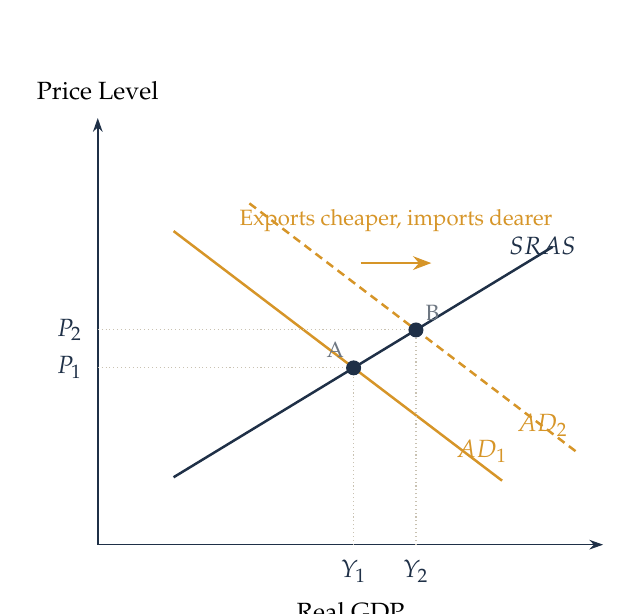
\begin{tikzpicture}[scale=1.0, baseline=(current bounding box.center)]
  \begin{axis}[
    econ chart,
    xlabel style={at={(ticklabel cs:0.5)}, anchor=north},
    width=8.0cm, height=7.0cm,
    xmin=0, xmax=100, ymin=0, ymax=100,
    xlabel={\small Real GDP},
    ylabel={\small Price Level},
    xtick={50.62,62.96}, xticklabels={$Y_1$,$Y_2$},
    ytick={41.44,50.33}, yticklabels={$P_1$,$P_2$},
  ]
    % Short-run aggregate supply curve
    \addplot[curve primary, domain=15:90] {0.72*x+5};
    \node[curve label, color=CurveNavy] at (axis cs:88,70) {$SRAS$};

    % Initial aggregate demand
    \addplot[curve accent, domain=15:80] {-0.9*x+87};
    \node[curve label, color=CurveGold] at (axis cs:76,22) {$AD_1$};

    % Shifted aggregate demand (depreciation shift)
    \addplot[curve accent shift, domain=30:95] {-0.9*x+107};
    \node[curve label, color=CurveGold] at (axis cs:88,28) {$AD_2$};

    % Initial equilibrium projection lines
    \addplot[guide projection] coordinates {(50.62,0)(50.62,41.44)};
    \addplot[guide projection] coordinates {(0,41.44)(50.62,41.44)};

    % New equilibrium projection lines
    \addplot[guide projection] coordinates {(62.96,0)(62.96,50.33)};
    \addplot[guide projection] coordinates {(0,50.33)(62.96,50.33)};

    % Equilibrium points
    \addplot[econ point, mark=*] coordinates {(50.62,41.44)};
    \node[annot, above left] at (50.62,41.44) {A};

    \addplot[econ point, mark=*] coordinates {(62.96,50.33)};
    \node[annot, above right] at (62.96,50.33) {B};

    % Shift arrow with cause label
    \draw[-{Stealth}, CurveGold, thick] (52,66) -- (66,66);
    \node[annot, CurveGold, above] at (59,71) {Exports cheaper, imports dearer};
  \end{axis}
\end{tikzpicture}%
}{%
\textbf{\color{NavyPrimary}Depreciation Impact}\\[4pt]
$\bullet$ Depreciation makes exports cheaper, imports dearer\\[2pt]
$\bullet$ Net exports (X-M) rise \(\rightarrow\) AD shifts right (AD\textsubscript{1} \(\rightarrow\) AD\textsubscript{2})\\[2pt]
$\bullet$ Real GDP rises (Y\textsubscript{1} \(\rightarrow\) Y\textsubscript{2}), price level rises (P\textsubscript{1} \(\rightarrow\) P\textsubscript{2})\\[2pt]
$\bullet$ Employment increases as firms hire to meet demand\\[2pt]
\textbf{\color{GoldAccent}Key:} Depreciation boosts AD via the net exports channel, but causes demand-pull inflation%
}
\end{diagrambox}

An increase in (X-M) is an injection into the circular flow, causing AD to shift right (AD\textsubscript{1} to AD\textsubscript{2}).

\textbf{Summary of Impacts:}
\begin{itemize}
  \item \textbf{National Income (Y):} Increases ($Y_1$ to $Y_2$).
  \item \textbf{Real Output:} Increases (movement towards potential GDP, reducing a negative output gap).
  \item \textbf{Price Level:} Rises ($P_1$ to $P_2$) -- demand-pull inflation.
  \item \textbf{Employment:} Increases, as firms hire more workers to meet the higher demand.
\end{itemize}

\subsubsection{Impact of an Appreciation (e.g.\ £ rises in value)}

\textbf{Mechanism:} A stronger pound makes UK exports more expensive (decreasing X) and imports cheaper (increasing M). Therefore, Net Exports (X-M) decrease.

A decrease in (X-M) is a withdrawal from the circular flow, causing AD to shift left (AD\textsubscript{1} to AD\textsubscript{2}).

\textbf{Summary of Impacts:}
\begin{itemize}
  \item \textbf{National Income (Y):} Decreases.
  \item \textbf{Real Output:} Decreases (increasing a negative output gap).
  \item \textbf{Price Level:} Falls ($P_1$ to $P_2$) -- disinflationary pressure.
  \item \textbf{Employment:} Decreases, as falling output leads to layoffs.
\end{itemize}

\begin{coreidea}
\textbf{Important Caveat:} The final impact on the price level also depends on costs. A depreciation makes imported raw materials and components more expensive, which can shift the AS curve to the left, creating cost-push inflation. For a thorough analysis, you should consider this secondary effect.
\end{coreidea}

\begin{evaluation}{Fixed vs. Floating Exchange Rate Systems}
\textbf{Strengths of Floating Rates:}
\begin{itemize}[leftmargin=*, nosep]
\item Automatic adjustment mechanism; deficits lead to depreciation, improving competitiveness without government action.
\item Monetary policy independence; central banks can set rates to suit domestic conditions, not defend a fixed rate.
\item No need for large foreign exchange reserves to defend the rate.
\end{itemize}
\textbf{Strengths of Fixed Rates:}
\begin{itemize}[leftmargin=*, nosep]
\item Certainty for traders and investors; exchange rate predictability reduces hedging costs.
\item Discipline on inflation; commitment to a fixed rate forces monetary discipline (no printing money).
\item Facilitates trade and investment in a currency union (e.g., Eurozone, before Brexit).
\end{itemize}
\textbf{Limitations:}
\begin{itemize}[leftmargin=*, nosep]
\item Floating rates can overshoot, creating volatility that harms trade; speculators destabilise the market.
\item Fixed rates require policy coordination; asymmetric shocks (e.g., German growth surge) create imbalances that force one country to adjust painfully.
\item Fixed rates are eventually abandoned in a crisis (devaluation); short-run cost, but inescapable if fundamentals are bad.
\end{itemize}
\textbf{It depends on\ldots}
\begin{itemize}[leftmargin=*, nosep]
\item Trade openness; small open economies with high trade may prefer the certainty of fixed rates or a currency union.
\item Symmetry of shocks; if trading partners face similar shocks, fixed rates work well; if asymmetric, floating rates allow faster adjustment.
\item Institutional credibility; if the central bank lacks credibility, a fixed-rate peg or currency board can anchor expectations.
\end{itemize}
\end{evaluation}

% ─────────────────────────────────────────────────────────────
\section{Policies to Correct Imbalances in the Current Account}

\subsection{Government Policy: Stability in the Current Account}

\begin{keyterm}{Stability in the Current Account}
A stable current account does not mean it is always zero or in perfect balance. Instead, it means it is \textbf{sustainable over the long run}. A small, persistent deficit can be sustainable if it is financed by long-term capital inflows for productive investment (e.g.\ foreign companies building factories). Instability arises when a deficit is large, persistent, and growing -- especially if it is financed by short-term ``hot'' money that can flee quickly.
\end{keyterm}

Think of your personal finances. It's stable to have a small, manageable credit card debt that you can pay off with your salary. It's unstable if your debt is huge and you're only paying the minimum balance, relying on new loans to survive.

Governments aim for current account stability to: prevent currency volatility; avoid a build-up of foreign debt; protect foreign exchange reserves; and maintain overall macroeconomic stability.

\subsection{The Effect of Policies on the Current Account}

The current account balance is broadly determined by: Exports (X) $-$ Imports (M). Policies aim to either increase exports or decrease imports.

\subsubsection{1.\ The Effect of Fiscal Policies}

\textbf{Expansionary Fiscal Policy (Increase G, Decrease T):}
\begin{itemize}
  \item Boosts AD and national income. With higher disposable income, consumers spend more, a significant portion of which goes on imported goods and services.
  \item \textbf{Result:} Imports (M) rise, which \textbf{worsens} the current account balance. This is a key reason why governments may avoid expansionary fiscal policy if the current account deficit is a major concern.
\end{itemize}

\textbf{Contractionary Fiscal Policy (Decrease G, Increase T):}
\begin{itemize}
  \item Reduces AD and national income. Consumers have less disposable income, so they cut back on spending, including on imports.
  \item \textbf{Result:} Imports (M) fall, which \textbf{improves} the current account balance.
\end{itemize}

\subsubsection{2.\ The Effect of Monetary Policies}

The effect works primarily through two channels: the Exchange Rate and Aggregate Demand.

\textbf{Contractionary Monetary Policy (Higher Interest Rates):}
\begin{itemize}
  \item \textbf{Exchange Rate Channel:} Higher interest rates attract hot money flows, increasing demand for the domestic currency and causing it to appreciate. A stronger currency makes exports more expensive (X $\downarrow$) and imports cheaper (M $\uparrow$). \textbf{Result: worsens the current account.}
  \item \textbf{Aggregate Demand Channel:} Higher interest rates discourage borrowing and spending, reducing AD and growth. Lower growth leads to lower demand for imports (M $\downarrow$). \textbf{Result: improves the current account.}
  \item \textbf{Net Effect:} Ambiguous and depends on time. In the short run, the AD effect is often quicker; in the long run, the exchange rate effect can badly damage export industries.
\end{itemize}

\textbf{Expansionary Monetary Policy (Lower Interest Rates):} Has the opposite, but also ambiguous, effects. A lower interest rate can weaken the currency (boosting X and reducing M) but also stimulate AD and demand for imports.

\subsubsection{3.\ The Effect of Supply-Side Policies}

These are long-term policies aimed at increasing the productive capacity and international competitiveness of the economy.

\textbf{How it improves the current account:}
\begin{itemize}
  \item \textbf{Lower Costs \& Prices:} Increased efficiency lowers production costs, allowing firms to offer more competitive prices on the world market, boosting exports (X $\uparrow$).
  \item \textbf{Higher Quality \& Innovation:} Investment in technology and skills leads to better quality products, increasing overseas demand for exports (X $\uparrow$).
  \item \textbf{Import Substitution:} As domestic industries become more efficient, they can produce goods closer to what consumers might otherwise import, reducing imports (M $\downarrow$).
\end{itemize}

\textbf{Evaluation:} The key drawback is that supply-side policies work with a very long time lag. They are not a solution for an immediate balance of payments crisis but are crucial for long-term structural improvement.

\subsubsection{4.\ The Effect of Protectionist Policies}

Protectionist tools include tariffs (taxes on imports), quotas (physical limits on imports), and subsidies to domestic exporters.

\textbf{How it improves the current account:}
\begin{itemize}
  \item Tariffs/Quotas make imported goods more expensive or less available, directly reducing the volume and value of imports (M $\downarrow$).
  \item Export Subsidies lower the cost for domestic firms to sell abroad, making them more competitive and increasing exports (X $\uparrow$).
\end{itemize}

\begin{coreidea}
\textbf{Evaluation (crucial for high marks):} While protectionism might seem like a direct solution, it has severe drawbacks. Other countries are likely to \textbf{retaliate} with their own tariffs on your exports. It protects inefficient domestic firms from competition, reducing the incentive to innovate. It leads to higher prices and less choice for consumers. And many protectionist measures violate WTO rules.
\end{coreidea}

\begin{tcolorbox}[enhanced,colback=EvalBg,colframe=EvalFrame,arc=0pt,boxrule=1pt,title={\bfseries\color{EvalFrame}Evaluation: Trade, Exchange Rates and the Balance of Payments},fonttitle=\small]
\small\RaggedRight
\begin{itemize}[itemsep=2pt,topsep=2pt]
  \item \textbf{Marshall-Lerner condition:} Depreciation improves the current account \textit{only if} $|PED_X| + |PED_M| > 1$. In the short run this condition often fails (inelastic demand) -- hence the J-curve: the current account \textit{worsens} before it improves.
  \item \textbf{Comparative advantage: assumptions matter:} The Ricardian model assumes no transport costs, perfect mobility of factors within countries, constant returns to scale, and no externalities. Relax any of these and free trade is less obviously beneficial.
  \item \textbf{Infant industry argument:} Temporary protection may be justified if the industry will eventually achieve comparative advantage. But governments often fail to remove protection once granted (``permanently temporary'').
  \item \textbf{Current account deficit sustainability:} A deficit is less concerning if it finances productive investment (future exports) rather than consumption. A deficit with a capital account surplus may reflect attractive investment conditions.
  \item \textbf{Fixed vs.\ floating:} A fixed rate provides certainty but requires large reserves and prevents independent monetary policy. Floating allows adjustment but creates uncertainty for traders and investors.
  \item \textbf{Expenditure-switching vs.\ expenditure-reducing:} Depreciation (expenditure-switching) may boost output; contractionary policy (expenditure-reducing) lowers output. Policymakers face a trade-off between correction and recession.
\end{itemize}
\end{tcolorbox}

\subsection{Exam Practice Questions -- Chapter 6}

\begin{exampractice}
\begin{enumerate}[leftmargin=*]
\item \textbf{``Explain the principle of comparative advantage and show why two countries can both gain from trade even if one country has an absolute advantage in both goods.''} [15 marks]
\textit{Model structure: Define absolute and comparative advantage using opportunity cost. Use numerical example with two countries and two goods. Show specialisation pattern and how both countries consume beyond their production possibility curve after trade. Explain terms of trade range.}

\item \textbf{``A car manufacturer imports steel at \pounds500 per tonne from abroad. The government imposes a 20\% tariff. Using a supply-and-demand diagram, show the effects on consumers, domestic producers, government revenue, and overall welfare.''} [15 marks]
\textit{Model structure: Draw S\&D for steel with horizontal world price. Show tariff raises domestic price. Shade and label: consumer surplus loss, producer surplus gain, government revenue rectangle, and deadweight loss triangles. Explain distribution of gains and losses.}

\item \textbf{``A country's currency appreciates following a sharp rise in interest rates. Using the AD/AS framework, explain the short-run effects on output, employment, and the price level, and evaluate policy options.''} [15 marks]
\textit{Model structure: Show appreciation reduces net exports, AD shifts left. Output falls, price level falls (disinflationary). But if caused by tight monetary policy fighting inflation, tight money is the goal. Discuss trade-off: inflation control vs. output loss. Supply-side policies needed for long-run growth.}

\item \textbf{``The UK has run a large current account deficit for many years. Analyse the causes and discuss policy options to correct this imbalance.''} [15 marks]
\textit{Model structure: Identify causes: strong domestic demand (high consumption and investment), weak productivity growth, deindustrialisation, strong currency (historically). Evaluate policies: depreciation (J-curve), supply-side reforms (raise competitiveness), fiscal contraction (reduce imports), protectionism (politically risky, invites retaliation). Discuss sustainability: is deficit sustainable if financed by FDI?}

\item \textbf{``Compare the advantages and disadvantages of a floating exchange rate system with those of a fixed exchange rate system. In your answer, consider the implications for monetary policy and trade.''} [15 marks]
\textit{Model structure: Floating: allows monetary independence, automatic adjustment via price changes, but exchange rate uncertainty. Fixed: provides certainty, anchors inflation expectations, but requires reserves, policy discipline, and can cause crises if misaligned. Discuss which suits small open economies vs. large economies; currency unions; shocks symmetry.}
\end{enumerate}
\end{exampractice}

% ============================================================
%  CHAPTER 7: THEORY OF THE FIRM
% ============================================================
\chapter{Theory of the Firm}

% ─────────────────────────────────────────────────────────────
\section{Utility}

\subsection{Definition and Calculation of Total Utility and Marginal Utility}

\begin{keyterm}{Total Utility (TU)}
The \textbf{total satisfaction} a consumer gets from consuming all units of a good within a given time period. It is the sum of the marginal utilities from each unit consumed: $TU = \sum MU$.
\end{keyterm}

Think of eating slices of pizza. Your Total Utility is the overall enjoyment you get from the entire meal.

\begin{keyterm}{Marginal Utility (MU)}
The \textbf{additional satisfaction} gained from consuming one more unit of a good.
\[ MU = \frac{\Delta TU}{\Delta Q} \]
where $\Delta TU$ = Change in Total Utility and $\Delta Q$ = Change in Quantity (= 1 for each successive unit). It is the extra enjoyment you get specifically from the 3rd slice of pizza, after already having eaten two.
\end{keyterm}

\begin{example}[Total Utility and Marginal Utility]
\begin{tabular}{@{}ccc@{}}
\textbf{Quantity (Q)} & \textbf{Total Utility (TU)} & \textbf{Marginal Utility (MU)} \\
\midrule
0 & 0  & -- \\
1 & 30 & 30 \\
2 & 55 & 25 \\
3 & 75 & 20 \\
4 & 90 & 15 \\
5 & 100 & 10 \\
\end{tabular}
\end{example}

\begin{coreidea}
As long as MU is positive, TU is increasing. When MU falls to zero, TU is at its maximum (the satiety point). If MU becomes negative (disutility), TU starts to fall.
\end{coreidea}

\subsection{Diminishing Marginal Utility}

\begin{keyterm}{Law of Diminishing Marginal Utility}
As a consumer consumes more and more units of a good in a given period of time, the additional (marginal) utility derived from each successive unit will \textbf{eventually diminish}.
\end{keyterm}

Using the pizza example: the first slice is extremely satisfying when you're hungry. The second is also great, but slightly less so. By the fourth or fifth slice, the extra satisfaction is much smaller. This is due to satiation.

The MU curve is downward sloping, illustrating this law. It is a fundamental reason why demand curves slope downwards.

\subsection{The Equi-Marginal Principle (Consumer Equilibrium)}

\begin{keyterm}{Consumer Equilibrium}
A rational consumer maximises their total utility when their limited income is allocated so that the last pound spent on each good yields the same marginal utility:
\[ \frac{MU_A}{P_A} = \frac{MU_B}{P_B} = \ldots \]
The ratio $MU/P$ is the \textbf{marginal utility per pound spent}.
\end{keyterm}

\textbf{Application -- Explaining Equilibrium:} If $MU_A/P_A > MU_B/P_B$, the consumer gains more satisfaction from the last pound spent on Good A. They should reallocate spending from Good B to Good A. As they buy more of A, its MU falls (due to diminishing MU). As they buy less of B, its MU rises. This continues until the ratios are equal. At this point, no reallocation can increase total utility -- consumer equilibrium is reached.

\begin{example}[Equi-Marginal Principle]
You have £10. A burger costs £5 and a cinema ticket costs £5.
\begin{itemize}
  \item If MU of a burger = 50 and MU of cinema = 25:
  \item Burger: $MU/P = 50/5 = 10$ utils per £
  \item Cinema: $MU/P = 25/5 = 5$ utils per £
\end{itemize}
You are not in equilibrium. You get more ``bang for your buck'' from burgers. The principle guides you towards the combination where the last £5 spent on each gives equal satisfaction.
\end{example}

\subsection{Derivation of an Individual Demand Curve}

The demand curve can be derived from marginal utility and the equi-marginal principle.

\begin{enumerate}
  \item \textbf{Start at a Price:} At a given price ($P_1$), a consumer adjusts their quantity purchased until $MU/P_1$ equals $MU/P$ for all other goods. This gives quantity $Q_1$ -- Point A on the demand curve.
  \item \textbf{Price Falls:} The price of the good falls to $P_2$.
  \item \textbf{Disequilibrium:} Now $MU/P_2 >$ $MU/P$ for other goods. The good now gives more marginal utility per pound spent. To restore equilibrium, the consumer buys more of this good.
  \item \textbf{Diminishing MU:} As they buy more, the MU of the good falls (Law of Diminishing MU).
  \item \textbf{New Equilibrium:} They stop buying more when MU (now lower) $/P_2$ is again equal to the $MU/P$ of other goods. This new, higher quantity is $Q_2$ -- Point B on the demand curve.
\end{enumerate}

By plotting ($P_1$, $Q_1$) and ($P_2$, $Q_2$), we trace out the individual's downward-sloping demand curve. The inverse relationship between price and quantity demanded is thus explained by diminishing MU and the pursuit of consumer equilibrium.

\subsection{Limitations of Marginal Utility Theory \& Assumptions of Rationality}

This theory makes strong assumptions about rational behaviour, which are often unrealistic.

\begin{itemize}
  \item \textbf{Consumers may not be capable of putting wants in rank order.} Utility is subjective and intangible. Can you precisely say you want a coffee ``2.4 times more'' than a tea? Wants are often vague, emotional, or influenced by complex psychological factors, not a clear, cardinal (numerical) ranking.
  \item \textbf{Consumers may not be capable of assigning a value for their satisfaction.} The theory assumes cardinal utility (utility can be measured in exact ``utils''). In reality, utility is ordinal -- we know we prefer A to B, but not by exactly how much. We cannot objectively quantify ``satisfaction''.
  \item \textbf{Consumers do not always behave rationally.} This is the most significant critique, drawing on Behavioural Economics:
  \begin{itemize}
    \item \textbf{Bounded Rationality:} Consumers lack the time, information, or mental processing power to constantly calculate $MU/P$ ratios. They use heuristics (mental shortcuts) and can make systematic errors.
    \item \textbf{Influence of Others:} Consumption is often social (Veblen goods, conspicuous consumption, bandwagon effect).
    \item \textbf{Habit \& Inertia:} People stick with what they know out of habit, not constant calculation.
    \item \textbf{Fairness \& Altruism:} Decisions are influenced by a sense of fairness or concern for others, not just personal utility maximisation.
    \item \textbf{Imperfect Information:} Choices are made with limited or asymmetric information, leading to sub-optimal decisions.
    \item \textbf{Impulsivity \& Weakness of Will:} People act against their own long-term interest (e.g., smoking, unhealthy eating).
  \end{itemize}
\end{itemize}

% ─────────────────────────────────────────────────────────────
\section{Indifference Curves and Budget Lines}

\subsection{The Basic Building Blocks: Indifference Curves \& Budget Lines}

\subsubsection{What is shown in an Indifference Curve?}

\begin{keyterm}{Indifference Curve}
An indifference curve maps all the combinations of two goods (e.g., apples and bananas) that give a consumer \textbf{equal satisfaction or utility}. The consumer is ``indifferent'' between any bundle on the same curve.
\end{keyterm}

\textbf{Key Properties:}
\begin{itemize}
  \item \textbf{Downward Sloping:} To maintain the same utility, if you get more of one good, you must give up some of the other.
  \item \textbf{Convex to the Origin:} This shape reflects the law of diminishing marginal rate of substitution (MRS). The MRS is the rate at which a consumer is willing to trade Good Y for Good X. As you have more X, you are willing to give up fewer units of Y to get even more X. This is why the slope gets flatter as you move right.
  \item \textbf{Higher Curves = Higher Utility:} An indifference curve further from the origin represents a higher level of satisfaction (more of both goods is better).
  \item \textbf{They Never Cross:} If they did, it would imply a logical inconsistency in consumer preferences.
\end{itemize}

\subsubsection{What is shown by a Budget Line?}

\begin{keyterm}{Budget Line}
The budget line (or budget constraint) shows all the possible combinations of two goods a consumer can afford, given their income and the prices of the goods:
\[ M = (P_x \times Q_x) + (P_y \times Q_y) \]
Its \textbf{slope} $= -(P_x / P_y)$: the relative price of the two goods, showing the market trade-off. The \textbf{intercepts} show the maximum quantity of one good if all income is spent on it ($M/P_x$ or $M/P_y$).
\end{keyterm}

\textbf{The Optimal Choice:} The consumer aims to reach the highest possible indifference curve that just touches their budget line. This occurs at the \textbf{tangency point}, where the slope of the indifference curve (MRS) equals the slope of the budget line (Price Ratio). Here, the consumer's subjective willingness to trade equals the market's ability to trade.


\begin{diagrambox}[Indifference Curves and Budget Line -- Consumer Equilibrium]
\diagramwithtext{%
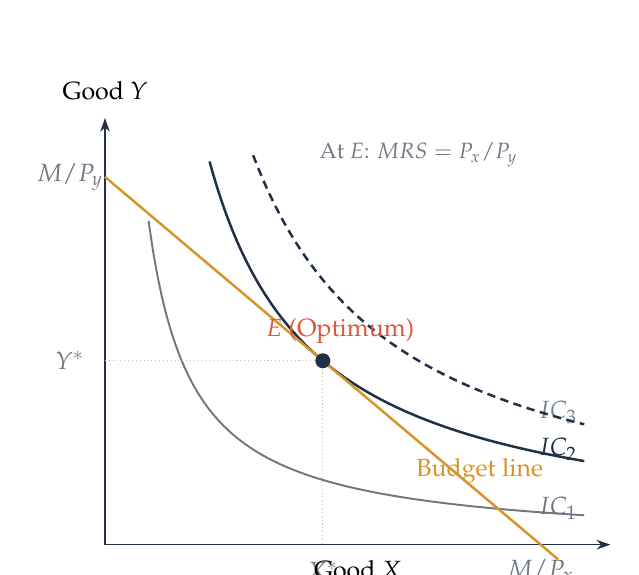
\begin{tikzpicture}[scale=1.0, baseline=(current bounding box.center)]
  \begin{axis}[econ chart,
    xlabel style={at={(ticklabel cs:0.5)}, anchor=north},
    width=8.0cm, height=7.0cm,
    xmin=0, xmax=5.8, ymin=0, ymax=5.8,
    xlabel={\small Good $X$},
    ylabel={\small Good $Y$},
    xtick=\empty, ytick=\empty
  ]
    % IC1 (lower utility)
    \addplot[curve muted, domain=0.5:5.5, samples=100] {2.2/x};
    \node[font=\small, color=AnnotGray] at (axis cs:5.2,0.5) {$IC_1$};

    % IC2 (optimal - tangent to budget line y=5-x at (2.5,2.5))
    \addplot[curve primary, domain=1.2:5.5, samples=100] {6.25/x};
    \node[font=\small, color=CurveNavy] at (axis cs:5.2,1.3) {$IC_2$};

    % IC3 (higher utility - unattainable)
    \addplot[curve primary shift, domain=1.7:5.5, samples=100] {9.0/x};
    \node[font=\small, color=CurveNavy, opacity=0.6] at (axis cs:5.2,1.8) {$IC_3$};

    % Budget line: from (0, 5.0) to (5.0, 0)
    \addplot[curve accent, domain=0:5.2, samples=2] {5 - x};
    \node[font=\small, color=CurveGold] at (axis cs:4.3,1.0) {Budget line};

    % Intercepts
    \node[font=\small, color=AnnotGray] at (axis cs:-0.4,5.0) {$M/P_y$};
    \node[font=\small, color=AnnotGray] at (axis cs:5.0,-0.35) {$M/P_x$};

    % Tangency point (optimal) = IC2 and budget line tangent at (2.5,2.5)
    \addplot[only marks, mark=*, mark size=2.5pt, color=AxisCharcoal] coordinates {(2.5,2.5)};

    % Guide projections to axes
    \addplot[guide projection] coordinates {(2.5,2.5)(2.5,0)};
    \addplot[guide projection] coordinates {(2.5,2.5)(0,2.5)};

    % Axis labels for optimal point
    \node[font=\small, color=AnnotGray] at (axis cs:2.5,-0.35) {$X^*$};
    \node[font=\small, color=AnnotGray] at (axis cs:-0.4,2.5) {$Y^*$};

    % Optimum label
    \node[font=\small, color=CurveRose] at (axis cs:2.7,2.9) {$E$ (Optimum)};

    % Condition note
    \node[font=\footnotesize, align=center, color=AnnotGray] at (axis cs:3.6,5.3) {At $E$: $MRS = P_x/P_y$};
  \end{axis}
\end{tikzpicture}%
}{%
\textbf{\color{NavyPrimary}Consumer Equilibrium}\\[4pt]
$\bullet$ IC\textsubscript{1} < IC\textsubscript{2} < IC\textsubscript{3} (higher = more utility)\\[2pt]
$\bullet$ Budget line shows affordable combinations given income and prices\\[2pt]
$\bullet$ Optimum at E: budget line tangent to IC\textsubscript{2} (highest attainable utility)\\[2pt]
$\bullet$ At E, MRS = P\textsubscript{x}/P\textsubscript{y} (marginal rate of substitution equals price ratio)\\[2pt]
$\bullet$ IC\textsubscript{3} is unattainable (above budget line)\\[2pt]
\textbf{\color{GoldAccent}Key:} Consumer maximises utility where the budget line is tangent to the highest reachable indifference curve%
}
\end{diagrambox}

\subsection{Causes of a Shift in the Budget Line}

A \textbf{shift} means the entire line moves. A \textbf{pivot} means one intercept moves while the other stays fixed.

\begin{itemize}
  \item \textbf{Increase in Income (Normal Goods):} The budget line shifts outwards parallelly. If income rises and prices stay the same, you can now afford more of both goods. Both intercepts ($M/P_x$ and $M/P_y$) increase. Consumers typically move to a higher indifference curve, consuming more of both normal goods.
  \item \textbf{Increase in Income (Inferior Goods):} The shift in the budget line is exactly the same (parallel outward shift). The difference lies in the consumer's response. For an inferior good (e.g., cheap supermarket own-brand bread), demand \emph{decreases} as income rises. So while the budget set expands, the consumer may choose to buy less of the inferior good and more of a normal/luxury good. You cannot see this from the budget line shift alone; you need the indifference curves to see the new chosen point.
\end{itemize}

\subsection{Income, Substitution \& Price Effects}

When the price of one good changes (e.g., Good X falls), the budget line pivots outward. The total change in quantity demanded (the \textbf{Price Effect}) can be split into two parts.

\subsubsection{The Substitution Effect}

\begin{keyterm}{Substitution Effect}
The change in consumption due to the change in \textbf{relative prices}, holding real income (utility) constant. It is \textbf{always negative} (non-positive): if the price of X falls, the substitution effect always leads to an increase in demand for X. Consumers substitute toward the now relatively cheaper good.
\end{keyterm}

To isolate it: imagine the price falls, but we artificially take away just enough of the consumer's income to put them back on their original indifference curve. The movement along the original curve to a point with the new slope (new price ratio) is the pure substitution effect.

\subsubsection{The Income Effect}

\begin{keyterm}{Income Effect}
The change in consumption due to the change in \textbf{purchasing power} (real income), holding relative prices constant at the new level. Its direction depends on the type of good: positive for normal goods, negative for inferior goods.
\end{keyterm}

To isolate it: now give back the ``imaginary'' income we took away. This causes a parallel shift from the ``substitution effect'' budget line to the actual new budget line. The movement from one indifference curve to another is the income effect.

\begin{example}[Combined Effects Table]
\begin{tabular}{@{}lllll@{}}
\textbf{Good Type} & \textbf{Sub. Effect} & \textbf{Income Effect} & \textbf{Price Effect} & \textbf{Demand Curve} \\
\midrule
Normal    & $\uparrow$ demand X & $\uparrow$ demand X & Strong increase & Downward sloping \\
Inferior  & $\uparrow$ demand X & $\downarrow$ demand X & Net increase (SE $>$ IE) & Downward sloping \\
Giffen    & $\uparrow$ demand X & Strong $\downarrow$ demand X & Net \textbf{decrease} (IE $>$ SE) & \textbf{Upward sloping} \\
\end{tabular}
\end{example}

\begin{coreidea}
\textbf{Key for Giffen Goods:} The perverse income effect is so strong (the good is a very strong inferior good, taking up a large part of the budget, like a staple food for the poor) that it overpowers the substitution effect. A fall in price increases real income so much that they buy less of the staple and switch to more desirable foods. This leads to an \textbf{upward-sloping demand curve}.
\end{coreidea}

\subsection{Limitations of the Indifference Curve Model}

\begin{itemize}
  \item \textbf{Consumers are not always rational:} The model assumes consistent, transitive preferences. In reality, consumers are influenced by bounded rationality (no time or brainpower to calculate optimal bundles), habit and impulse (choices are often habitual or made at the checkout), and social and psychological factors (advertising, peer pressure, fairness, and framing effects).
  \item \textbf{Choice is between just two goods:} The model is a major simplification. In reality, consumers allocate income across thousands of goods. While the principles can be extended mathematically, the simple 2D diagram ignores complex trade-offs and complementary relationships between multiple goods.
  \item \textbf{A theoretical, impractical concept:} Indifference curves represent internal preferences which cannot be seen or measured directly. We can't ask consumers to map them out. In practice, economists work backward using \textbf{revealed preference} -- observed consumer choices -- to infer what their indifference maps might look like, but they can never be precisely modelled for a real individual.
\end{itemize}

% ─────────────────────────────────────────────────────────────
\section{Efficiency and Market Failure}

\subsection{Definitions and Conditions for Efficiency}

\subsubsection{Productive Efficiency}

\begin{keyterm}{Productive Efficiency}
Producing goods and services at the \textbf{lowest possible cost}. No resources are wasted.
\begin{itemize}
  \item \textbf{For a Firm:} Occurs at the point of minimum Average Total Cost (ATC) -- the lowest point on the U-shaped ATC curve.
  \item \textbf{For an Economy:} The economy is on its Production Possibility Frontier (PPF). It is impossible to produce more of one good without producing less of another.
\end{itemize}
\end{keyterm}

\subsubsection{Allocative Efficiency}

\begin{keyterm}{Allocative Efficiency}
Resources are allocated according to consumer preferences. The mix of goods and services produced is exactly what society wants. It occurs when:
\[ P = MC \]
\textbf{Why?} Price (P) represents the value to the consumer (Marginal Social Benefit). Marginal Cost (MC) represents the cost to society of producing that last unit. If P $>$ MC, more should be produced. If P $<$ MC, less should be produced. Only where P = MC is the welfare-maximising quantity produced.
\end{keyterm}

\subsubsection{Economic Efficiency}

The umbrella term that combines both productive and allocative efficiency. An economically efficient market produces the right goods (allocative), using the best methods (productive), at the right time.

\subsection{Pareto Optimality}

\begin{keyterm}{Pareto Optimality}
Named after economist Vilfredo Pareto. A situation is Pareto optimal (or Pareto efficient) when it is \textbf{impossible to make one person better off without making at least one other person worse off}.
\end{keyterm}

In theory, perfect competition leads to a Pareto optimal outcome because it achieves both productive (min ATC) and allocative (P = MC) efficiency. Any reallocation of resources away from this point would benefit someone at the expense of someone else.

\begin{coreidea}
\textbf{Important Note:} Pareto optimality does not consider fairness or equality. A situation where one person owns everything could be Pareto optimal if taking anything from them makes them worse off.
\end{coreidea}

\subsection{Dynamic Efficiency}

\begin{keyterm}{Dynamic Efficiency}
Efficiency \textbf{over time}. It refers to the ability of a firm or market to innovate, improve technology, and develop new products in the long run. Key drivers include investment in R\&D, innovation, human capital training, and the development of new production processes.
\end{keyterm}

\begin{coreidea}
\textbf{Key Trade-off:} The market structure best for dynamic efficiency might not be perfect competition. While perfect competition is statically efficient (productive + allocative), firms in competitive markets often have supernormal profits too low to fund expensive R\&D. Monopolies or oligopolies may have more profit to reinvest, potentially making them more dynamically efficient in the long run, even though they are less allocatively efficient in the short run. This is a key evaluation point.
\end{coreidea}

\subsection{Market Failure: Definition and Reasons}

\begin{keyterm}{Market Failure}
Market failure occurs when the free market, left to its own devices (the price mechanism), \textbf{fails to allocate resources efficiently}. It results in a loss of economic and social welfare. In other words, the market outcome is not Pareto optimal.
\end{keyterm}

\subsubsection{Reasons for Market Failure}

\begin{itemize}
  \item \textbf{Externalities (Positive \& Negative):} The private costs/benefits of an economic activity differ from the social costs/benefits. This creates a divergence between the private and social optimum, leading to over-production (negative externality, e.g., pollution) or under-production (positive externality, e.g., vaccination).
  \item \textbf{Merit and Demerit Goods:}
  \begin{itemize}
    \item \emph{Merit Goods} (e.g., education, healthcare): The market under-provides them because consumers undervalue their long-term private benefits (information failure) and they have positive externalities.
    \item \emph{Demerit Goods} (e.g., cigarettes, excessive sugar): The market over-provides them because consumers overvalue private benefits or are unaware of harms (information failure) and they have negative externalities.
  \end{itemize}
  \item \textbf{Public Goods:} Have two key characteristics -- \emph{non-excludable} (cannot prevent non-payers from consuming) and \emph{non-rivalrous} (one person's consumption does not reduce availability for others). The \textbf{free-rider problem} means no private firm will provide them as they cannot charge and make a profit. They are missing markets. \emph{Quasi-public goods} have some but not all of these characteristics (e.g., a toll road is excludable but non-rival up to the congestion point).
  \item \textbf{Information Failure (Asymmetric Information):} When one party in a transaction has more or better information than the other, leading to suboptimal decisions. This includes \emph{adverse selection} (``hidden information'' before a transaction, e.g., the used car ``lemons'' problem) and \emph{moral hazard} (``hidden action'' after a transaction, e.g., becoming a less careful driver after getting car insurance).
  \item \textbf{Abuse of Monopoly Power:} When a firm with significant market power restricts output to force up prices. This leads to allocative inefficiency (P $>$ MC) and productive inefficiency due to ``X-inefficiency'' (lack of competitive pressure). There is a clear welfare loss to society.
\end{itemize}

% ─────────────────────────────────────────────────────────────
\section{Private Costs and Benefits, Externalities and Social Costs and Benefits}

\subsection{Social Costs and Benefits -- The Core Framework}

\begin{keyterm}{The Social Cost/Benefit Framework}
\begin{itemize}
  \item \textbf{Private Costs (PC):} Costs incurred by the economic decision-maker (e.g., a firm's rent, wages, materials).
  \item \textbf{External Costs (EC):} Costs imposed on third parties not involved in the transaction (e.g., pollution, noise, health problems). Not paid by the producer/consumer.
  \item \textbf{Social Costs (SC):} The total cost to society: $SC = PC + EC$
  \item \textbf{Private Benefits (PB):} Benefits received by the economic decision-maker (e.g., a firm's revenue; a consumer's utility).
  \item \textbf{External Benefits (EB):} Benefits enjoyed by third parties (e.g., herd immunity from vaccinations, a skilled workforce).
  \item \textbf{Social Benefits (SB):} The total benefit to society: $SB = PB + EB$
\end{itemize}
\end{keyterm}

\subsubsection{The ``Marginal'' Concept -- Key for Diagrams}

``Marginal'' means one more unit. It is about the costs/benefits of producing or consuming the next unit.

\begin{itemize}
  \item \textbf{Marginal Private Cost (MPC):} The cost to the producer of making one more unit. This is their supply curve.
  \item \textbf{Marginal Social Cost (MSC):} $MSC = MPC + MEC$. If there is a negative externality, $MSC > MPC$.
  \item \textbf{Marginal Private Benefit (MPB):} The benefit to the consumer of consuming one more unit. This is their demand curve.
  \item \textbf{Marginal Social Benefit (MSB):} $MSB = MPB + MEB$. If there is a positive externality, $MSB > MPB$.
\end{itemize}

\subsection{Positive and Negative Externalities}

\begin{keyterm}{Externality}
A cost or benefit that affects a \textbf{third party} who did not choose to incur that cost or benefit. It is a side effect of an economic transaction.
\end{keyterm}

\begin{example}[Examples of Externalities by Category]
\begin{tabular}{@{}>{\RaggedRight\arraybackslash}p{0.13\linewidth}>{\RaggedRight\arraybackslash}p{0.4\linewidth}>{\RaggedRight\arraybackslash}p{0.4\linewidth}@{}}
 & \textbf{Consumption Externality} & \textbf{Production Externality} \\
\midrule
\textbf{Positive} (MSB $>$ MPB) & \textbf{Education:} You benefit (better job), but society also benefits (more informed citizens, lower crime, innovation). \textbf{Vaccinations:} You get protected and also reduce disease spread (herd immunity). & \textbf{Bee-keeping:} The firm sells honey (private benefit), but bees pollinate nearby orchards for free (external benefit). \textbf{R\&D:} A firm invents something, but knowledge spills over to other firms/industries. \\
\textbf{Negative} (MSC $>$ MPC) & \textbf{Driving a Petrol Car:} You get transport (private benefit), but cause air pollution and congestion for others (external cost). \textbf{Smoking:} Your satisfaction vs.\ others' passive smoking. & \textbf{Chemical Manufacturing:} The firm pays for inputs (private cost), but pollutes a river, harming fisheries and communities (external cost). \textbf{Noise from Factories/Construction.} \\
\end{tabular}
\end{example}

\subsection{Deadweight Welfare Loss (DWL)}

\begin{keyterm}{Deadweight Welfare Loss (DWL)}
The loss of economic efficiency when the equilibrium quantity is not the socially optimal quantity. It represents a net loss of total welfare (consumer + producer surplus) for society. On a diagram, it always appears as a \textbf{triangle}.
\end{keyterm}

\textbf{From a Negative Externality (e.g., Pollution):}
\begin{itemize}
  \item \textbf{Market Outcome:} Firms only consider MPC. Equilibrium is where MPB = MPC (at $Q_m$, $P_m$).
  \item \textbf{Socially Optimal:} Where MSB = MSC. Because MSC $>$ MPC, this is at a \emph{lower} quantity ($Q_{opt}$).
  \item \textbf{The Problem:} The market \textbf{over-produces} ($Q_m > Q_{opt}$).
  \item \textbf{The DWL:} The triangle between $Q_{opt}$ and $Q_m$, bounded by the MSC and MSB curves. This area represents the net cost to society of producing those extra units (where social cost $>$ social benefit).
\end{itemize}

\textbf{From a Positive Externality (e.g., Education):}
\begin{itemize}
  \item \textbf{Market Outcome:} Consumers only consider MPB. Equilibrium is where MPB = MPC (at $Q_m$, $P_m$).
  \item \textbf{Socially Optimal:} Where MSB = MSC. Because MSB $>$ MPB, this is at a \emph{higher} quantity ($Q_{opt}$).
  \item \textbf{The Problem:} The market \textbf{under-produces} ($Q_m < Q_{opt}$).
  \item \textbf{The DWL:} The triangle between $Q_m$ and $Q_{opt}$, bounded by the MSB and MPC curves. This area represents the net benefit to society lost by not producing those units (where social benefit $>$ social cost).
\end{itemize}


\begin{diagrambox}[Negative Production Externality]
\diagramwithtext{%
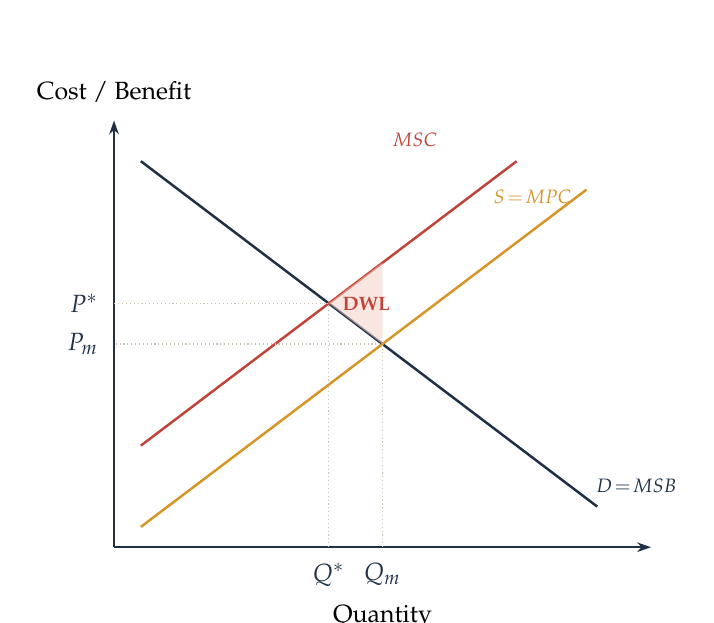
\begin{tikzpicture}[baseline=(current bounding box.center)]
  \begin{axis}[econ chart, width=8.4cm, height=7.0cm,
    xmin=0, xmax=100, ymin=0, ymax=105,
    xlabel={\small Quantity},
    ylabel={\small Cost / Benefit},
    xlabel style={at={(ticklabel cs:0.5)}, anchor=north},
    xtick={40,50}, xticklabels={$Q^*$,$Q_m$},
    ytick={50,60}, yticklabels={$P_m$,$P^*$}
  ]
    % Demand = MSB (navy, downward sloping)
    \addplot[curve primary, domain=5:90] {-x + 100};
    \node[font=\scriptsize\itshape, color=CurveNavy, anchor=west]
        at (axis cs:88,15) {$D\!=\!MSB$};
    % Private supply = MPC (gold)
    \addplot[curve accent, domain=5:88] {x};
    \node[font=\scriptsize\itshape, color=CurveGold, anchor=south east]
        at (axis cs:87,82) {$S\!=\!MPC$};
    % Social supply = MSC (red, lies above MPC due to external cost)
    \addplot[curve danger, domain=5:75] {x + 20};
    \node[font=\scriptsize\itshape, color=CurveDanger, anchor=south east]
        at (axis cs:62,96) {$MSC$};
    % Projection lines + DWL triangle
    \addplot[guide projection] coordinates {(40,0)(40,60)(0,60)};
    \addplot[guide projection] coordinates {(50,0)(50,50)(0,50)};
    \fill[FillNegative, opacity=0.55]
        (axis cs:40,60) -- (axis cs:50,70) -- (axis cs:50,50) -- cycle;
    \node[font=\scriptsize\bfseries, color=CurveDanger] at (axis cs:47,60) {DWL};
  \end{axis}
\end{tikzpicture}%
}{%
\textbf{\color{NavyPrimary}Reading the diagram:}\\[4pt]
Firms weigh only private cost $MPC$.\\[2pt]
Market settles at $Q_m$ where $MPC = MSB$.\\[2pt]
Production imposes an external cost on others, so true $MSC$ lies above $MPC$.\\[2pt]
Socially optimal output $Q^*$ (where $MSC = MSB$) is \emph{smaller} than $Q_m$.\\[2pt]
The red triangle is the deadweight loss from overproduction.\\[2pt]
Remedy: a tax on production shifts $MPC$ up toward $MSC$.%
}
\end{diagrambox}

\begin{diagrambox}[Positive Production Externality]
\diagramwithtext{%
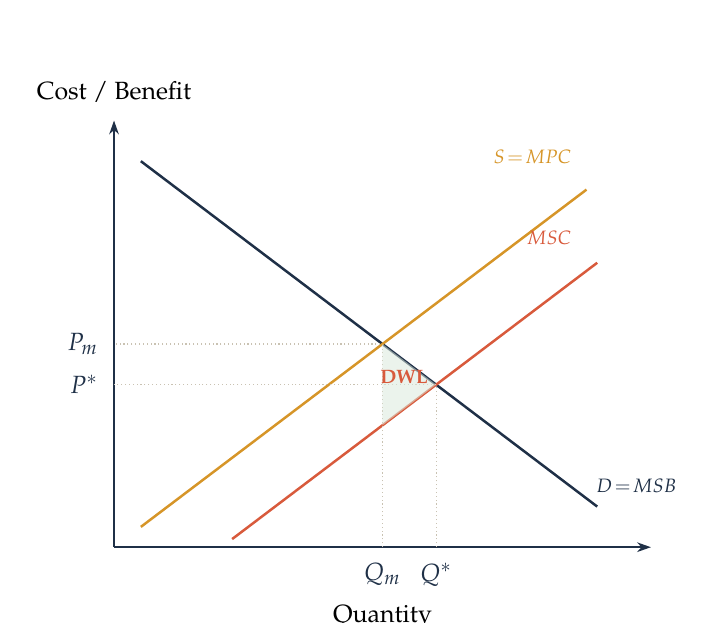
\begin{tikzpicture}[baseline=(current bounding box.center)]
  \begin{axis}[econ chart, width=8.4cm, height=7.0cm,
    xmin=0, xmax=100, ymin=0, ymax=105,
    xlabel={\small Quantity},
    ylabel={\small Cost / Benefit},
    xlabel style={at={(ticklabel cs:0.5)}, anchor=north},
    xtick={50,60}, xticklabels={$Q_m$,$Q^*$},
    ytick={40,50}, yticklabels={$P^*$,$P_m$}
  ]
    \addplot[curve primary, domain=5:90] {-x + 100};
    \node[font=\scriptsize\itshape, color=CurveNavy, anchor=west]
        at (axis cs:88,15) {$D\!=\!MSB$};
    \addplot[curve accent, domain=5:88] {x};
    \node[font=\scriptsize\itshape, color=CurveGold, anchor=south east]
        at (axis cs:87,92) {$S\!=\!MPC$};
    % MSC lies BELOW MPC by 20 (external benefit makes social cost lower)
    \addplot[curve secondary, domain=22:90] {x - 20};
    \node[font=\scriptsize\itshape, color=CurveRose, anchor=south east]
        at (axis cs:87,72) {$MSC$};
    \addplot[guide projection] coordinates {(50,0)(50,50)(0,50)};
    \addplot[guide projection] coordinates {(60,0)(60,40)(0,40)};
    \fill[FillPositive, opacity=0.55]
        (axis cs:50,50) -- (axis cs:60,40) -- (axis cs:50,30) -- cycle;
    \node[font=\scriptsize\bfseries, color=CurveRose] at (axis cs:54,42) {DWL};
  \end{axis}
\end{tikzpicture}%
}{%
\textbf{\color{NavyPrimary}Reading the diagram:}\\[4pt]
The market settles at $Q_m$ where $MPC = MSB$.\\[2pt]
Production generates an external benefit (e.g.\ R\&D spillovers), so true $MSC$ lies \emph{below} $MPC$.\\[2pt]
Socially optimal output $Q^*$ is \emph{larger} than $Q_m$.\\[2pt]
The pink triangle is the deadweight loss from underproduction.\\[2pt]
Remedy: a production subsidy shifts $MPC$ down toward $MSC$.%
}
\end{diagrambox}

\begin{diagrambox}[Negative Consumption Externality]
\diagramwithtext{%
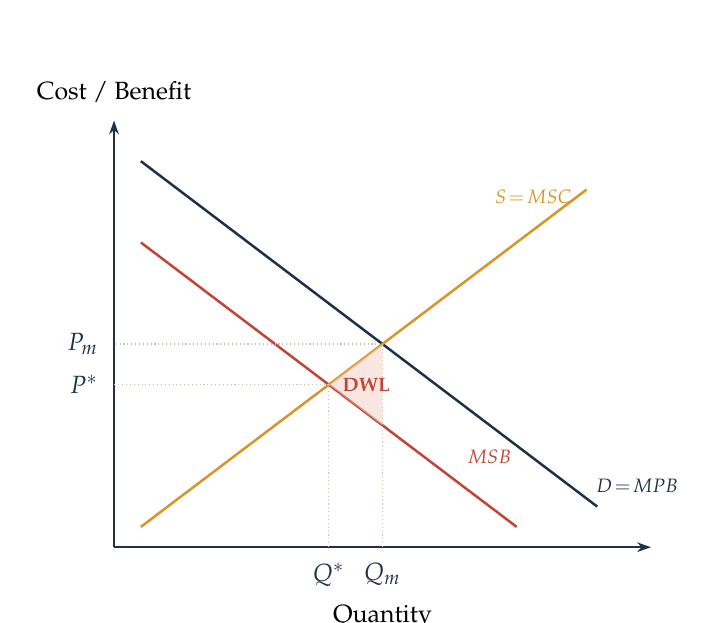
\begin{tikzpicture}[baseline=(current bounding box.center)]
  \begin{axis}[econ chart, width=8.4cm, height=7.0cm,
    xmin=0, xmax=100, ymin=0, ymax=105,
    xlabel={\small Quantity},
    ylabel={\small Cost / Benefit},
    xlabel style={at={(ticklabel cs:0.5)}, anchor=north},
    xtick={40,50}, xticklabels={$Q^*$,$Q_m$},
    ytick={40,50}, yticklabels={$P^*$,$P_m$}
  ]
    \addplot[curve primary, domain=5:90] {-x + 100};
    \node[font=\scriptsize\itshape, color=CurveNavy, anchor=west]
        at (axis cs:88,15) {$D\!=\!MPB$};
    % MSB lies BELOW MPB (external cost lowers true benefit)
    \addplot[curve danger, domain=5:75] {-x + 80};
    \node[font=\scriptsize\itshape, color=CurveDanger, anchor=south west]
        at (axis cs:64,18) {$MSB$};
    \addplot[curve accent, domain=5:88] {x};
    \node[font=\scriptsize\itshape, color=CurveGold, anchor=south east]
        at (axis cs:87,82) {$S\!=\!MSC$};
    \addplot[guide projection] coordinates {(40,0)(40,40)(0,40)};
    \addplot[guide projection] coordinates {(50,0)(50,50)(0,50)};
    \fill[FillNegative, opacity=0.55]
        (axis cs:40,40) -- (axis cs:50,50) -- (axis cs:50,30) -- cycle;
    \node[font=\scriptsize\bfseries, color=CurveDanger] at (axis cs:47,40) {DWL};
  \end{axis}
\end{tikzpicture}%
}{%
\textbf{\color{NavyPrimary}Reading the diagram:}\\[4pt]
Consumers buy at $Q_m$ where private benefit $MPB = MSC$.\\[2pt]
Consumption imposes an external cost, so true $MSB$ lies \emph{below} $MPB$.\\[2pt]
Socially optimal consumption $Q^*$ (where $MSB = MSC$) is \emph{smaller} than $Q_m$.\\[2pt]
The red triangle is the deadweight loss from overconsumption.\\[2pt]
Remedy: a consumption tax shifts $MPB$ down toward $MSB$.%
}
\end{diagrambox}

\begin{diagrambox}[Positive Consumption Externality]
\diagramwithtext{%
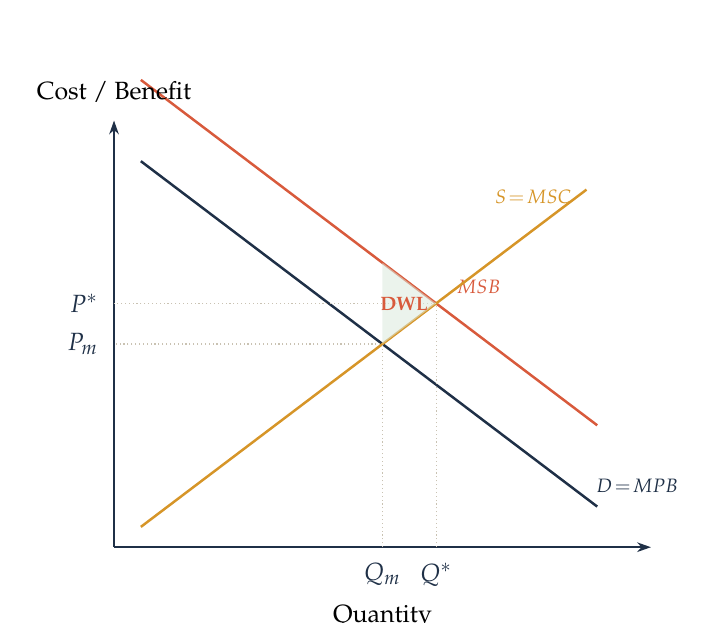
\begin{tikzpicture}[baseline=(current bounding box.center)]
  \begin{axis}[econ chart, width=8.4cm, height=7.0cm,
    xmin=0, xmax=100, ymin=0, ymax=105,
    xlabel={\small Quantity},
    ylabel={\small Cost / Benefit},
    xlabel style={at={(ticklabel cs:0.5)}, anchor=north},
    xtick={50,60}, xticklabels={$Q_m$,$Q^*$},
    ytick={50,60}, yticklabels={$P_m$,$P^*$}
  ]
    \addplot[curve primary, domain=5:90] {-x + 100};
    \node[font=\scriptsize\itshape, color=CurveNavy, anchor=west]
        at (axis cs:88,15) {$D\!=\!MPB$};
    % MSB lies ABOVE MPB (external benefit raises true benefit)
    \addplot[curve secondary, domain=5:90] {-x + 120};
    \node[font=\scriptsize\itshape, color=CurveRose, anchor=south west]
        at (axis cs:62,60) {$MSB$};
    \addplot[curve accent, domain=5:88] {x};
    \node[font=\scriptsize\itshape, color=CurveGold, anchor=south east]
        at (axis cs:87,82) {$S\!=\!MSC$};
    \addplot[guide projection] coordinates {(50,0)(50,50)(0,50)};
    \addplot[guide projection] coordinates {(60,0)(60,60)(0,60)};
    \fill[FillPositive, opacity=0.55]
        (axis cs:50,70) -- (axis cs:60,60) -- (axis cs:50,50) -- cycle;
    \node[font=\scriptsize\bfseries, color=CurveRose] at (axis cs:54,60) {DWL};
  \end{axis}
\end{tikzpicture}%
}{%
\textbf{\color{NavyPrimary}Reading the diagram:}\\[4pt]
Consumers buy at $Q_m$ where private benefit $MPB = MSC$.\\[2pt]
Consumption generates an external benefit (e.g.\ vaccination), so true $MSB$ lies \emph{above} $MPB$.\\[2pt]
Socially optimal consumption $Q^*$ is \emph{larger} than $Q_m$.\\[2pt]
The pink triangle is the deadweight loss from underconsumption.\\[2pt]
Remedy: a consumption subsidy shifts $MPB$ up toward $MSB$.%
}
\end{diagrambox}


\subsection{Asymmetric Information \& Moral Hazard}

\begin{keyterm}{Asymmetric Information}
When one party in a transaction has \textbf{more or better information} than the other. This undermines fair and efficient markets. Examples: a used car seller knows the car's faults; a doctor knows more about necessary treatments than a patient; an insurance buyer knows more about their risky lifestyle than the insurer.
\end{keyterm}

\begin{keyterm}{Moral Hazard}
A specific consequence of asymmetric information. It occurs when an individual or firm, once \textbf{protected from risk} (e.g., by insurance), changes their behaviour to become more risky or less careful because they know they won't bear the full cost. Examples: driving more recklessly because you have comprehensive car insurance; a bank taking huge risks because it expects a government bailout (``too big to fail'').
\end{keyterm}

Moral Hazard creates a negative externality. The risky behaviour of the insured party can ultimately raise costs for everyone else in the insurance pool (higher premiums) or for taxpayers (in the case of bailouts).

\subsection{Cost-Benefit Analysis (CBA)}

\begin{keyterm}{Cost-Benefit Analysis (CBA)}
A practical tool used by governments to evaluate major projects (e.g., a new airport, hospital, or high-speed rail) by considering \textbf{all social costs and benefits}, not just private ones. CBA tries to put a monetary value on all projected costs and benefits over time, including externalities (e.g., valuing lost green space, time saved for commuters, reduced pollution) which the free market ignores.
\end{keyterm}

\textbf{The Process:}
\begin{enumerate}
  \item Identify all costs (PC + EC) and benefits (PB + EB).
  \item Quantify them in monetary terms as far as possible (this is the difficult, controversial part).
  \item Compare the Total Social Benefits (TSB) and Total Social Costs (TSC).
\end{enumerate}

\textbf{Benefit:Cost Ratio} $= \frac{\text{Total Social Benefits}}{\text{Total Social Costs}}$

\begin{itemize}
  \item If B:C Ratio $>$ 1: The project yields a net social gain. Benefits outweigh costs.
  \item If B:C Ratio $<$ 1: The project yields a net social loss. Costs outweigh benefits.
\end{itemize}

\textbf{Limitations:} Valuing intangibles (e.g., a view, wildlife), accuracy of forecasts, choosing the correct discount rate for future values, and subjectivity.

% ─────────────────────────────────────────────────────────────
\section{Costs, Revenue, and Production Theory}

\subsection{Short-Run Production Function}

\begin{keyterm}{Short Run vs.\ Long Run}
The \textbf{short run} is a period where at least one factor of production is fixed (usually capital/factory space). The \textbf{long run} is a period where all factors are variable.
\end{keyterm}

\begin{example}[Product Measures]
\begin{tabular}{@{}lll@{}}
\textbf{Term} & \textbf{Definition} & \textbf{Formula} \\
\midrule
Total Product (TP) & Total output produced & $TP = Q$ \\
Average Product (AP) & Output per unit of variable factor & $AP = TP \div L$ \\
Marginal Product (MP) & Extra output from one more unit of variable factor & $MP = \Delta TP \div \Delta L$ \\
\end{tabular}
\end{example}

\begin{keyterm}{Law of Diminishing Returns (Law of Variable Proportions)}
As more units of a variable factor are added to fixed factors, the marginal product will \textbf{eventually diminish}. Why? Fixed factors become overcrowded -- more workers share the same machines/space. The MP curve rises initially (specialisation), peaks, then falls. The AP curve follows MP.
\end{keyterm}

\subsection{Short-Run Cost Function}

\begin{example}[Short-Run Cost Definitions]
\begin{tabular}{@{}>{\RaggedRight\arraybackslash}p{0.20\linewidth}>{\RaggedRight\arraybackslash}p{0.44\linewidth}>{\RaggedRight\arraybackslash}p{0.27\linewidth}@{}}
\textbf{Cost Type} & \textbf{Definition} & \textbf{Formula} \\
\midrule
Total Fixed Cost (TFC) & Costs that don't vary with output (rent, salaries) & TFC = constant \\
Total Variable Cost (TVC) & Costs that vary with output (raw materials, wages) & TVC = f(Q) \\
Total Cost (TC) & All costs of production & TC = TFC + TVC \\
Average Fixed Cost (AFC) & Fixed cost per unit & AFC = TFC/Q \\
Average Variable Cost (AVC) & Variable cost per unit & AVC = TVC/Q \\
Average Total Cost (ATC) & Total cost per unit & ATC = TC/Q = AFC + AVC \\
Marginal Cost (MC) & Cost of producing one more unit & MC = $\Delta$TC/$\Delta$Q \\
\end{tabular}
\end{example}

\textbf{Why the U-Shape? (Critical for Diagrams)}
\begin{itemize}
  \item \textbf{AFC:} Always downward-sloping (spreading fixed costs over more units).
  \item \textbf{AVC \& ATC:} U-shaped because they initially fall due to increasing returns (specialisation, better factor utilisation), then eventually rise as diminishing returns sets in -- more variable inputs are needed per extra unit of output.
\end{itemize}

\textbf{Key Relationships:} MC cuts AVC and ATC at their minimum points. When MC $<$ AVC/ATC, average costs are falling. When MC $>$ AVC/ATC, average costs are rising.


\needspace{15\baselineskip}
\begin{diagrambox}[Short-Run Cost Curves: AFC, AVC, ATC and MC]
\diagramwithtext{%
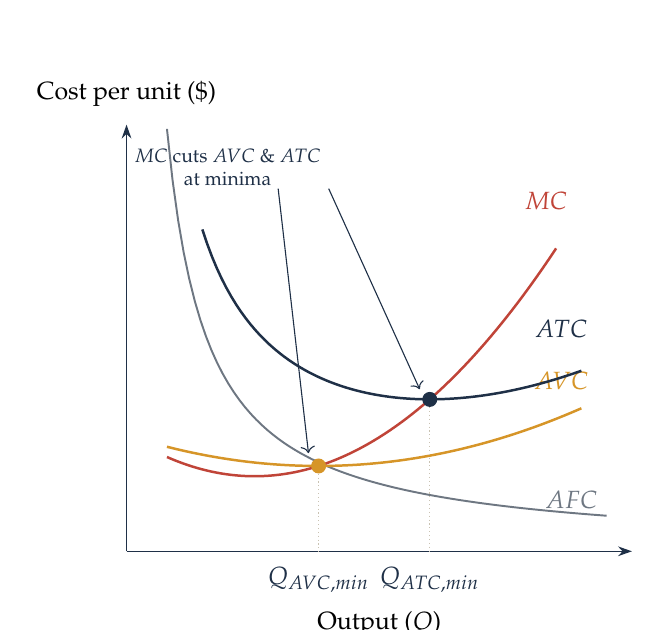
\begin{tikzpicture}[scale=1.0, baseline=(current bounding box.center)]
  \begin{axis}[econ chart,
    xlabel style={at={(ticklabel cs:0.5)}, anchor=north},
    width=8.0cm, height=7.0cm,
    xmin=0, xmax=100, ymin=0, ymax=100,
    xlabel={\small Output ($Q$)},
    ylabel={\small Cost per unit (\$)},
    xtick={38,60}, xticklabels={$Q_{AVC,min}$, $Q_{ATC,min}$},
    ytick=\empty
  ]
    % Derived from TC = 0.005Q³ - 0.38Q² + 27.22Q + 792
    % AVC = 0.005Q² - 0.38Q + 27.22 (min at Q=38, value=20)
    % MC = dTC/dQ = 0.015Q² - 0.76Q + 27.22 (min at Q=25.3, value=17.6)
    % ATC = AVC + AFC = 0.005Q² - 0.38Q + 27.22 + 792/Q (min at Q≈60, value≈35.6)
    % MC(38) = 0.015*1444 - 28.88 + 27.22 = 20 = AVC(38) ✓
    % MC(60) = 0.015*3600 - 45.6 + 27.22 = 35.62 = ATC(60) ✓
    % ATC = AVC + AFC by construction ✓

    % AFC -- hyperbola (always falling)
    \addplot[curve muted, domain=8:95, samples=80] {792/x};
    \node[font=\small, color=AnnotGray] at (axis cs:88,12) {$AFC$};

    % AVC -- U-shape
    \addplot[curve accent, domain=8:90, samples=80] {0.005*x^2 - 0.38*x + 27.22};
    \node[font=\small, color=CurveGold] at (axis cs:86,40) {$AVC$};

    % ATC -- U-shape (= AVC + AFC, always above AVC)
    \addplot[curve primary, domain=15:90, samples=80] {0.005*x^2 - 0.38*x + 27.22 + 792/x};
    \node[font=\small, color=CurveNavy] at (axis cs:86,52) {$ATC$};

    % MC -- U-shape, cuts AVC and ATC at their minima
    \addplot[curve danger, domain=8:85, samples=80] {0.015*x^2 - 0.76*x + 27.22};
    \node[font=\small, color=CurveDanger] at (axis cs:83,82) {$MC$};

    % Min AVC point: Q=38, AVC=MC=20
    \addplot[guide projection] coordinates {(38,20)(38,0)};
    \addplot[only marks, mark=*, mark size=2.5pt, color=CurveGold] coordinates {(38,20)};

    % Min ATC point: Q=60, ATC=MC≈35.6
    \addplot[guide projection] coordinates {(60,35.6)(60,0)};
    \addplot[only marks, mark=*, mark size=2.5pt, color=CurveNavy] coordinates {(60,35.6)};

    % Annotations
    \node[font=\scriptsize, align=center, color=CurveNavy] at (axis cs:20,90) {$MC$ cuts $AVC$ \& $ATC$\\at minima};
    \draw[->, thin, color=CurveNavy] (axis cs:30,85) -- (axis cs:36,23);
    \draw[->, thin, color=CurveNavy] (axis cs:40,85) -- (axis cs:58,38);
  \end{axis}
\end{tikzpicture}%
}{%
\textbf{\color{NavyPrimary}Key relationships:}\\[4pt]
\textbf{\color{CurveGold}MC} crosses \textbf{\color{CurveGold}AVC} and \textbf{\color{CurveNavy}ATC} at their minimum points. AFC always falls. U-shape arises from increasing returns (falling costs) initially, then diminishing returns (rising costs) as output expands.%
}
\end{diagrambox}


\subsection{Long-Run Production \& Costs}

In the long run, all factors are variable. Firms can change factory size, machinery, everything.

\begin{keyterm}{Returns to Scale}
What happens to output when all inputs change proportionally.
\end{keyterm}

\begin{example}[Returns to Scale]
\begin{tabular}{@{}lll@{}}
\textbf{Type} & \textbf{When inputs double...} & \textbf{Effect on LRAC} \\
\midrule
Increasing Returns to Scale & Output more than doubles & LRAC falls \\
Constant Returns to Scale & Output exactly doubles & LRAC constant \\
Decreasing Returns to Scale & Output less than doubles & LRAC rises \\
\end{tabular}
\end{example}

\begin{keyterm}{Long-Run Average Cost (LRAC) Curve}
U-shaped (but flatter than the SRAC). The downward portion reflects economies of scale; the upward portion reflects diseconomies of scale. The \textbf{Minimum Efficient Scale (MES)} is the lowest output where minimum LRAC is achieved. Firms must reach this to be competitive.
\end{keyterm}

\textbf{SRAC vs.\ LRAC -- The ``Envelope'' Curve:} Each SRAC curve represents a different fixed plant size. The LRAC is the ``envelope'' of all possible SRAC curves -- the lowest possible cost for each output level. At the tangency points: to the left of MES, the SRAC is tangent to the LRAC at the falling portion; at MES, the SRAC is tangent at its minimum point; to the right of MES, the SRAC is tangent at the rising portion.


\begin{diagrambox}[Long-Run Average Cost (LRAC) -- The Envelope Curve]
\diagramwithtext{%
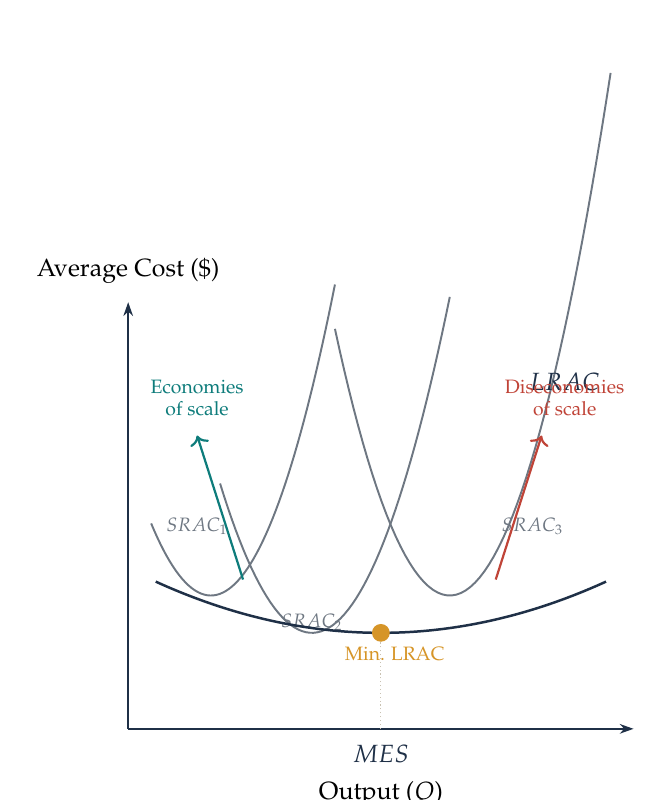
\begin{tikzpicture}[scale=1.0, baseline=(current bounding box.center)]
  \begin{axis}[econ chart,
    xlabel style={at={(ticklabel cs:0.5)}, anchor=north},
    width=8.0cm, height=7.0cm,
    xmin=0, xmax=110, ymin=0, ymax=80,
    xlabel={\small Output ($Q$)},
    ylabel={\small Average Cost (\$)},
    xtick={55}, xticklabels={$MES$},
    ytick=\empty
  ]
    % SRAC curves (3 sizes) - muted
    \addplot[curve muted, domain=5:45, samples=60] {0.08*(x-18)^2 + 25};
    \addplot[curve muted, domain=20:70, samples=60] {0.07*(x-40)^2 + 18};
    \addplot[curve muted, domain=45:105, samples=60] {0.08*(x-70)^2 + 25};

    \node[font=\scriptsize, color=AnnotGray] at (axis cs:15,38) {$SRAC_1$};
    \node[font=\scriptsize, color=AnnotGray] at (axis cs:40,20) {$SRAC_2$};
    \node[font=\scriptsize, color=AnnotGray] at (axis cs:88,38) {$SRAC_3$};

    % LRAC envelope (overall U-shape) - primary
    \addplot[curve primary, domain=6:104, samples=120] {0.004*(x-55)^2 + 18};
    \node[font=\small\bfseries, color=CurveNavy] at (axis cs:95,65) {$LRAC$};

    % MES dashed line
    \addplot[guide projection] coordinates {(55,0)(55,18)};
    \addplot[only marks, mark=*, mark size=3pt, color=CurveGold] coordinates {(55,18)};
    \node[font=\scriptsize, color=CurveGold] at (axis cs:58,14) {Min. LRAC};

    % Arrows and labels for economies / diseconomies
    \draw[->, thick, color=CurveSage] (axis cs:25,28) -- (axis cs:15,55);
    \node[font=\scriptsize, color=CurveSage, align=center] at (axis cs:15,62) {Economies\\of scale};

    \draw[->, thick, color=CurveDanger] (axis cs:80,28) -- (axis cs:90,55);
    \node[font=\scriptsize, color=CurveDanger, align=center] at (axis cs:95,62) {Diseconomies\\of scale};
  \end{axis}
\end{tikzpicture}%
}{%
\textbf{\color{NavyPrimary}The envelope principle:}\\[4pt]
LRAC is the \textbf{\color{CurveRose}lowest-cost} option for each output. Left of MES: economies of scale (larger scale lowers cost). At MES: minimum LRAC reached. Right of MES: diseconomies (managerial complexity, rising costs).%
}
\end{diagrambox}


\subsection{Economies \& Diseconomies of Scale}

\subsubsection{Internal Economies of Scale}

\begin{example}[Internal Economies of Scale]
\begin{tabular}{@{}lll@{}}
\textbf{Type} & \textbf{Explanation} & \textbf{Example} \\
\midrule
Technical & Larger, more efficient machinery; specialisation & Assembly line \\
Purchasing & Bulk-buying discounts & Supermarket chains \\
Marketing & Advertising costs spread over more units & Coca-Cola ads \\
Managerial & Specialist managers (HR, Finance, etc.) & Large corporations \\
Financial & Better loan rates (less risky) & Blue-chip companies \\
Risk-bearing & Diversify products/markets & Conglomerates \\
\end{tabular}
\end{example}

\subsubsection{External Economies of Scale}

Cost advantages from industry growth (not the firm itself): concentration of specialised suppliers and labour pools (e.g., Silicon Valley); shared industry research and knowledge (e.g., pharmaceutical hubs); and local training colleges and universities (e.g., film schools near Hollywood).

\subsubsection{Internal Diseconomies of Scale}

Communication problems (bureaucracy, slow decisions); motivation and coordination issues (worker alienation); control and monitoring costs (more layers of management needed).

\subsubsection{External Diseconomies of Scale}

Congestion (traffic, pollution) as the industry grows too large; competition for resources driving up wages and land prices; over-specialisation making firms vulnerable to industry-wide shocks.

\subsection{Revenue Concepts}

\begin{example}[Revenue Definitions]
\begin{tabular}{@{}>{\RaggedRight\arraybackslash}p{0.17\linewidth}>{\RaggedRight\arraybackslash}p{0.32\linewidth}>{\RaggedRight\arraybackslash}p{0.17\linewidth}>{\RaggedRight\arraybackslash}p{0.24\linewidth}@{}}
\textbf{Term} & \textbf{Definition} & \textbf{Formula} & \textbf{Notes} \\
\midrule
Total Revenue (TR) & Total money from sales & TR = P $\times$ Q & \\
Average Revenue (AR) & Revenue per unit sold & AR = TR/Q = Price & In competitive markets, AR is constant \\
Marginal Revenue (MR) & Extra revenue from one more unit & MR = $\Delta$TR/$\Delta$Q & Key for profit maximisation (MR = MC) \\
\end{tabular}
\end{example}

In perfectly competitive markets, AR = MR = Price (a horizontal line).

\subsection{Profit Concepts}

\begin{keyterm}{Normal Profit}
The \textbf{minimum profit} needed to keep a firm in the industry. In economic terms, it is actually a cost (the opportunity cost of the entrepreneur's resources). It occurs when TR = TC (including all opportunity costs). Accounting profit just covers what entrepreneurs could earn elsewhere.
\end{keyterm}

\begin{keyterm}{Supernormal Profit (Abnormal/Economic Profit)}
Profit \textbf{above} normal profit (TR $>$ TC where TC includes normal profit). It signals that the industry is attractive and new firms will want to enter.
\end{keyterm}

\begin{keyterm}{Subnormal Profit}
Profit \textbf{below} normal profit (TR $<$ TC where TC includes normal profit). The industry is unattractive and firms will want to exit. In economic terms, this is often called a ``loss''.
\end{keyterm}

\textbf{Practical Calculation:}
\begin{itemize}
  \item Accounting Profit = TR $-$ Explicit Costs (rent, wages, materials, etc.)
  \item Economic Profit = TR $-$ (Explicit Costs + Implicit/Opportunity Costs)
  \item Normal Profit: Economic Profit = 0 \quad Supernormal: Economic Profit $>$ 0 \quad Subnormal: Economic Profit $<$ 0
\end{itemize}

% ─────────────────────────────────────────────────────────────
\section{Different Market Structures}

\subsection{The Meaning and Structure of Market Structures}

\begin{keyterm}{Market Structure}
The organisational and competitive characteristics of a market -- the ``environment'' in which firms operate. Defined by: number of firms; product differentiation; barriers to entry; control over prices (price maker vs.\ price taker); and availability of information.
\end{keyterm}

\begin{example}[Market Structure Comparison]
\scriptsize
\begin{tabular}{@{}>{\RaggedRight\arraybackslash}p{0.12\linewidth}>{\RaggedRight\arraybackslash}p{0.12\linewidth}>{\RaggedRight\arraybackslash}p{0.18\linewidth}>{\RaggedRight\arraybackslash}p{0.12\linewidth}>{\RaggedRight\arraybackslash}p{0.11\linewidth}>{\RaggedRight\arraybackslash}p{0.18\linewidth}@{}}
\textbf{Feature} & \textbf{Perfect Comp.} & \textbf{Monopolistic Comp.} & \textbf{Oligopoly} & \textbf{Monopoly} & \textbf{Natural Monopoly} \\
\midrule
Firms & Very many & Many & Few (2--20) dominant & One & One \\
Product & Homogeneous & Differentiated & Homogeneous or diff. & Unique & Unique \\
Barriers & None & Low & High & Very high & Extremely high \\
Price control & Price taker & Some control & Significant (interdep.) & Substantial & Significant (regulated) \\
Information & Perfect & Imperfect & Imperfect, asymmetric & Imperfect & Imperfect \\
Examples & Wheat, forex & Restaurants, hairdressers & Supermarkets, banking & Patented drug & Water, rail, electricity \\
\end{tabular}
\normalsize
\end{example}

\subsection{Barriers to Entry and Exit}

Barriers are obstacles that protect incumbent firms and prevent new competitors from entering easily. High barriers = less competition.

\begin{itemize}
  \item \textbf{Legal Barriers:} Patents, copyrights, licences (e.g., taxi medallions), government franchise.
  \item \textbf{Market Barriers:} Brand loyalty, advertising, control over essential resources or distribution channels.
  \item \textbf{Cost Barriers:} Huge sunk costs (non-recoverable investments like R\&D and advertising), economies of scale that favour large existing firms.
  \item \textbf{Physical Barriers:} Ownership of a key resource (e.g., a mine, a prime location).
  \item \textbf{Barriers to Exit:} Costs of leaving a market. Sunk costs are a major barrier to exit -- because you can't recover them, you might stay in the market even if making losses, to avoid writing them off completely.
\end{itemize}

\subsection{Performance of Firms in Different Structures}

\subsubsection{Perfect Competition (PC) -- The Benchmark}

The demand curve is perfectly elastic (horizontal) at the market price (AR = MR = D).

\begin{itemize}
  \item \textbf{Short Run:} Can make supernormal profit, normal profit, or a loss. Operates where MC = MR.
  \item \textbf{Long Run:} Only normal profit is made. Freedom of entry/exit means supernormal profits attract new firms, increasing supply and lowering price until profits are normal.
  \item \textbf{Efficiency:} Productively efficient (min AC) and allocatively efficient (P = MC) in the long run. X-inefficiency is unlikely due to competitive pressure.
  \item \textbf{Shutdown:} In the short run, if price $<$ AVC. In the long run, if price $<$ AC.
  \item \textbf{Supply Curve:} The firm's MC curve above AVC.
\end{itemize}

\subsubsection{Monopoly}

\begin{itemize}
  \item \textbf{Revenue Curves:} Downward sloping AR (demand) and MR curves. MR lies below AR.
  \item \textbf{Profits:} Can make long-run supernormal profit due to barriers to entry.
  \item \textbf{Efficiency:} Not productively or allocatively efficient (P $>$ MC, leading to deadweight welfare loss). Can be X-inefficient due to lack of competition.
  \item \textbf{Shutdown:} In the long run, will shut down if price $<$ AC.
\end{itemize}

\subsubsection{Monopolistic Competition}

\begin{itemize}
  \item \textbf{Like monopoly in SR:} Downward sloping demand curve; can make supernormal profit.
  \item \textbf{Like PC in LR:} Low barriers mean new firms enter with similar products, stealing demand. The firm's demand curve shifts left until it is just tangent to the AC curve -- resulting in only normal profit in the long run.
  \item \textbf{Excess Capacity:} In the long run, firms operate at an output less than the one that would minimise AC (not productively efficient).
\end{itemize}

\subsubsection{Oligopoly -- The Game Theory Market}

\begin{keyterm}{Oligopoly: Key Feature -- Interdependence}
Each firm's decisions depend on the expected reactions of rivals. This leads to non-price competition (advertising, branding, loyalty schemes) to avoid triggering a price war.
\end{keyterm}

\begin{itemize}
  \item \textbf{Collusion:} Firms may cooperate (formally or tacitly) to act like a monopoly, restrict output, and raise prices (e.g., cartels like OPEC).
  \item \textbf{Kinked Demand Curve Model:} Explains price rigidity. Firms fear a price increase won't be matched (they lose sales, so demand is elastic above the current price), but a price decrease will be matched by rivals (they gain few customers, so demand is inelastic below the current price). This creates a kink at the prevailing price and a gap (discontinuity) in the MR curve. Even if costs change (MC shifts up or down within the gap), the profit-maximising price and output remain the same. This explains price ``stickiness'' in oligopolies.
  \item \textbf{Prisoner's Dilemma:} A game theory model showing why cooperation (collusion) is unstable. Even if it is best for all to collude, the individual incentive to cheat (cut price, increase output) leads to a worse outcome for all. This explains price wars.
\end{itemize}

\subsubsection{Contestable Markets}

\begin{keyterm}{Contestable Market}
A market is contestable if there are no sunk costs and entry/exit is costless and quick (e.g., an airline route). Even a monopoly or oligopoly will behave competitively -- keeping prices low and efficiency high -- due to the threat of ``hit-and-run'' entry by new firms. Barriers to entry are more important than the current number of firms.
\end{keyterm}

\textbf{Market Structures in Practice:} The textbook distinction between structures is cleaner than reality. Few markets are purely competitive or purely monopolistic -- most lie on a spectrum. Monopolistic competition may look inefficient on static criteria (excess capacity, P $>$ MC), but the product variety it generates has real value to consumers that standard welfare analysis ignores. Oligopolies can be fiercely competitive (supermarkets) or tacitly collusive (petrol stations), depending on the specific industry and regulatory environment. The contestability argument suggests that what matters for efficiency is not the number of firms but the threat of entry -- a single incumbent facing credible entry threats may behave more competitively than a fragmented market with high sunk costs. Monopoly itself is not always harmful: where significant economies of scale exist (natural monopoly), a single large firm can produce at lower cost than several small ones. The critical question then becomes regulation, not structure. Dynamic efficiency further complicates the picture -- monopoly profits can fund research and development, potentially benefiting consumers in the long run through innovation. Empirically, the relationship between market concentration and consumer welfare is ambiguous; case-by-case analysis of specific industries, their cost structures, and the threat of entry typically yields more insight than blanket judgements about market structure.

\begin{diagrambox}[Perfect Competition (Short Run) -- Supernormal Profit]
\diagramwithtext{%
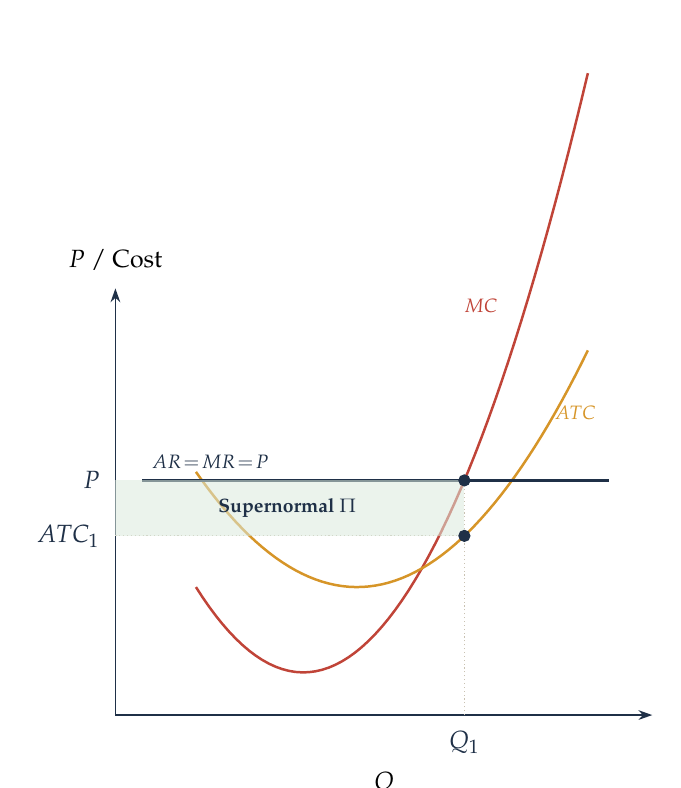
\begin{tikzpicture}[baseline=(current bounding box.center)]
  \begin{axis}[econ chart,
    width=8.4cm, height=7.0cm,
    xmin=0, xmax=100, ymin=0, ymax=100,
    xlabel={\small $Q$}, ylabel={\small $P$ / Cost},
    xlabel style={at={(ticklabel cs:0.5)}, anchor=north},
    xtick={65}, xticklabels={$Q_1$},
    ytick={42,55}, yticklabels={$ATC_1$,$P$}
  ]
    \addplot[curve danger, domain=15:88, samples=60] {0.05*(x-35)^2 + 10};
    \node[font=\scriptsize, color=CurveDanger, anchor=south east] at (axis cs:73,92) {$MC$};
    \addplot[curve accent, domain=15:88, samples=60] {0.03*(x-45)^2 + 30};
    \node[font=\scriptsize, color=CurveGold, anchor=south west] at (axis cs:80,67) {$ATC$};
    % AR=MR=P (horizontal): use curve primary so it shares the navy ink
    % with the "demand" convention used elsewhere in the book.
    \addplot[curve primary, domain=5:92] {55};
    \node[font=\scriptsize\itshape, color=CurveNavy, anchor=south west]
        at (axis cs:5,55.5) {$AR\!=\!MR\!=\!P$};
    \addplot[guide projection] coordinates {(65,0)(65,55)};
    \addplot[guide projection] coordinates {(0,42)(65,42)};
    \addplot[only marks, mark=*, mark size=2pt, color=AxisCharcoal]
        coordinates {(65,55)(65,42)};
    \fill[FillPositive, opacity=0.55] (axis cs:0,42) rectangle (axis cs:65,55);
    \node[font=\scriptsize\bfseries, color=CurveNavy] at (axis cs:32,48.5) {Supernormal $\Pi$};
  \end{axis}
\end{tikzpicture}%
}{%
\textbf{\color{CurveNavy}Reading the diagram:} the firm is a price-taker, so $AR=MR=P$ is a horizontal line.  Output $Q_1$ is set where $MC=MR$.  Because $P>ATC_1$ at that output, the shaded rectangle is \textit{supernormal profit}.\\[5pt]
Free entry then attracts new firms; market supply shifts right, the price line falls until only normal profit remains.%
}
\end{diagrambox}

\begin{diagrambox}[Perfect Competition (Long Run) -- Normal Profit]
\diagramwithtext{%
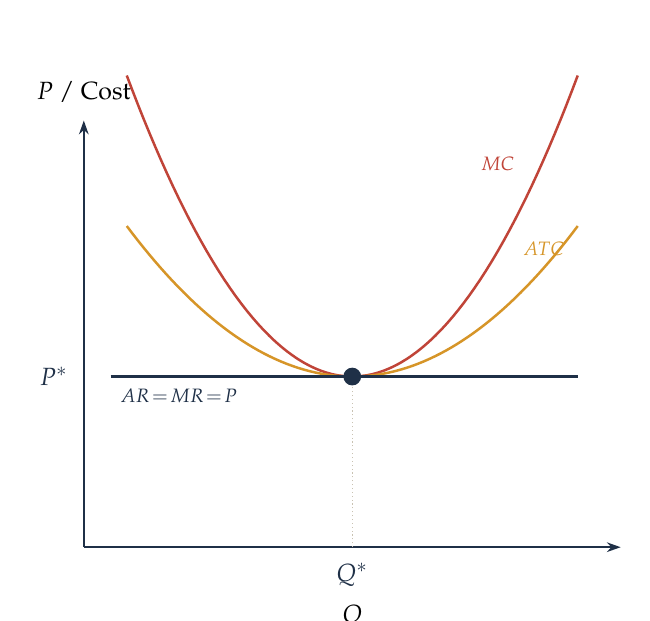
\begin{tikzpicture}[baseline=(current bounding box.center)]
  \begin{axis}[econ chart,
    width=8.4cm, height=7.0cm,
    xmin=0, xmax=100, ymin=0, ymax=100,
    xlabel={\small $Q$}, ylabel={\small $P$ / Cost},
    xlabel style={at={(ticklabel cs:0.5)}, anchor=north},
    xtick={50}, xticklabels={$Q^*$},
    ytick={40}, yticklabels={$P^*$}
  ]
    % MC and ATC tangent at the same point (50, 40) so all four curves meet.
    \addplot[curve danger, domain=8:92, samples=80] {0.04*(x-50)^2 + 40};
    \node[font=\scriptsize, color=CurveDanger, anchor=south east] at (axis cs:82,86) {$MC$};
    \addplot[curve accent, domain=8:92, samples=80] {0.02*(x-50)^2 + 40};
    \node[font=\scriptsize, color=CurveGold, anchor=south west] at (axis cs:80,66) {$ATC$};
    \addplot[curve primary, domain=5:92] {40};
    \node[font=\scriptsize\itshape, color=CurveNavy, anchor=north west]
        at (axis cs:5,39.5) {$AR\!=\!MR\!=\!P$};
    \addplot[guide projection] coordinates {(50,0)(50,40)};
    \addplot[only marks, mark=*, mark size=3pt, color=CurveNavy] coordinates {(50,40)};
    % The tangency at this dot is explained in full in the sidebar — no
    % inline callout needed, which kept colliding with the dipping curves.
  \end{axis}
\end{tikzpicture}%
}{%
\textbf{\color{CurveNavy}Long-run equilibrium:} entry has driven price down until $AR=MR$ is tangent to $ATC$ at its minimum.  All four curves -- $MC$, $ATC$, $AR$ and $MR$ -- meet at $(Q^*,P^*)$.  Firms earn only \textit{normal profit}.\\[5pt]
The outcome is both \textbf{allocatively efficient} ($P=MC$) and \textbf{productively efficient} (output at minimum $ATC$) -- the textbook benchmark.%
}
\end{diagrambox}

\begin{diagrambox}[Perfect Competition (Short Run) -- Subnormal Profit (Loss)]
\diagramwithtext{%
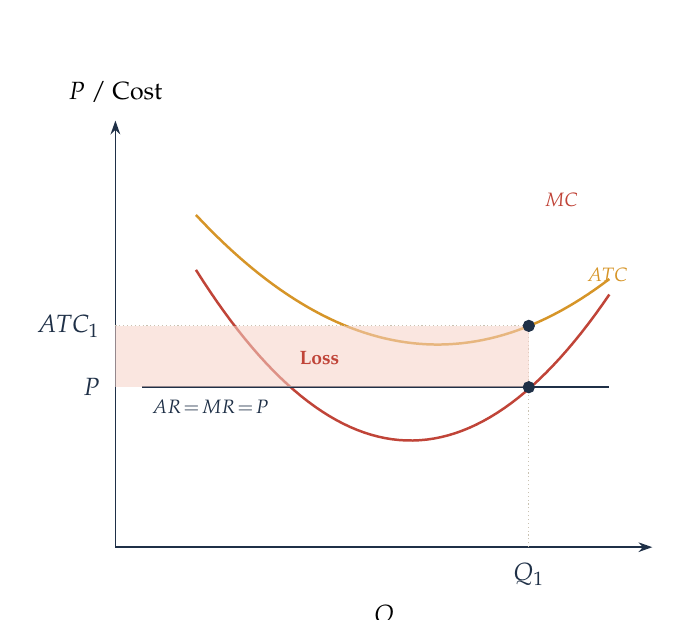
\begin{tikzpicture}[baseline=(current bounding box.center)]
  \begin{axis}[econ chart,
    width=8.4cm, height=7.0cm,
    xmin=0, xmax=100, ymin=0, ymax=80,
    xlabel={\small $Q$}, ylabel={\small $P$ / Cost},
    xlabel style={at={(ticklabel cs:0.5)}, anchor=north},
    xtick={77}, xticklabels={$Q_1$},
    ytick={30,41.5}, yticklabels={$P$,$ATC_1$}
  ]
    \addplot[curve danger, domain=15:92, samples=60] {0.02*(x-55)^2 + 20};
    \node[font=\scriptsize, color=CurveDanger, anchor=south east] at (axis cs:88,62) {$MC$};
    \addplot[curve accent, domain=15:92, samples=60] {0.012*(x-60)^2 + 38};
    \node[font=\scriptsize, color=CurveGold, anchor=south west] at (axis cs:86,48) {$ATC$};
    \addplot[curve primary, domain=5:92] {30};
    % Price line sits below the loss rectangle — label below the line keeps
    % it out of the shaded region and prevents collision with "Loss".
    \node[font=\scriptsize\itshape, color=CurveNavy, anchor=north west]
        at (axis cs:5,29.5) {$AR\!=\!MR\!=\!P$};
    \addplot[guide projection] coordinates {(77,0)(77,41.5)};
    \addplot[guide projection] coordinates {(0,41.5)(77,41.5)};
    \addplot[only marks, mark=*, mark size=2pt, color=AxisCharcoal] coordinates {(77,30)(77,41.5)};
    \fill[FillNegative, opacity=0.55] (axis cs:0,30) rectangle (axis cs:77,41.5);
    \node[font=\scriptsize\bfseries, color=CurveDanger] at (axis cs:38,35.5) {Loss};
  \end{axis}
\end{tikzpicture}%
}{%
\textbf{\color{CurveNavy}Reading the diagram:} the firm still produces at $Q_1$ (where $MC=MR$) -- but the market price has fallen below average total cost, so $P<ATC_1$.  The shaded red rectangle is the firm's loss.\\[5pt]
The firm continues to operate in the short run provided $P\geq AVC$ (covers its variable costs).  In the long run, loss-making firms exit; market supply shifts left, and price rises back to normal-profit level.%
}
\end{diagrambox}



\begin{diagrambox}[Monopoly -- Supernormal Profit and Deadweight Welfare Loss]
\diagramwithtext{%
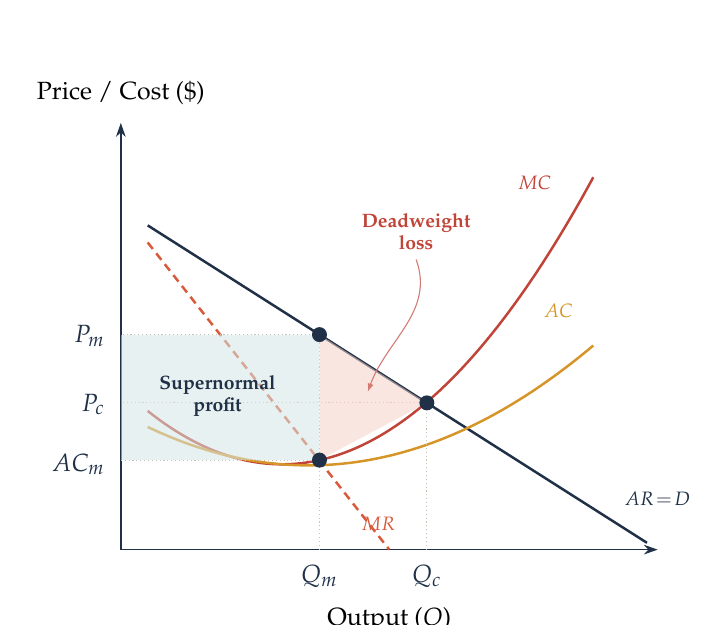
\begin{tikzpicture}[baseline=(current bounding box.center)]
  \begin{axis}[econ chart,
    width=8.4cm, height=7.0cm,
    xmin=0, xmax=100, ymin=0, ymax=100,
    xlabel={\small Output ($Q$)},
    ylabel={\small Price / Cost (\$)},
    xlabel style={at={(ticklabel cs:0.5)}, anchor=north},
    xtick={37,57}, xticklabels={$Q_m$,$Q_c$},
    ytick={20,34,50}, yticklabels={$AC_m$,$P_c$,$P_m$}
  ]
    % --- AR (Demand) -------------------------------------------------
    \addplot[curve primary, domain=5:98] {-0.8*x + 80};
    \node[font=\scriptsize\itshape, color=CurveNavy, anchor=west]
        at (axis cs:92,12) {$AR\!=\!D$};
    % --- MR (dashed, half-slope of AR) ------------------------------
    \addplot[curve secondary, densely dashed, domain=5:50] {-1.6*x + 80};
    \node[font=\scriptsize\itshape, color=CurveRose, anchor=west]
        at (axis cs:43,6) {$MR$};
    % --- MC (U-shape) -----------------------------------------------
    %  0.02*x^2 - 1.2*x + 38   (min at x=30, value 20)
    \addplot[curve danger, domain=5:88, samples=80] {0.02*x^2 - 1.2*x + 38};
    \node[font=\scriptsize, color=CurveDanger, anchor=south east]
        at (axis cs:82,82) {$MC$};
    % --- AC (U-shape) -----------------------------------------------
    %  0.01*x^2 - 0.7*x + 32   (min at x=35)
    \addplot[curve accent, domain=5:88, samples=80] {0.01*x^2 - 0.7*x + 32};
    \node[font=\scriptsize, color=CurveGold, anchor=south east]
        at (axis cs:86,52) {$AC$};
    % --- Equilibrium markers ---------------------------------------
    %  Monopoly:  Q_m=37, P_m=50.4, AC_m≈21 (from MC at Q_m)
    \addplot[guide projection] coordinates {(37,0)(37,50.4)(0,50.4)};
    \addplot[guide projection] coordinates {(37,20.98)(0,20.98)};
    %  Competitive (P=MC):  Q_c=57, P_c=34.4
    \addplot[guide projection] coordinates {(57,0)(57,34.4)(0,34.4)};
    \addplot[only marks, mark=*, mark size=2.5pt, color=AxisCharcoal]
        coordinates {(37,50.4)(57,34.4)(37,20.98)};
    % --- Supernormal-profit rectangle ------------------------------
    \fill[FillPrimary, opacity=0.55]
        (axis cs:0,20.98) rectangle (axis cs:37,50.4);
    \node[font=\scriptsize\bfseries, color=CurveNavy, align=center]
        at (axis cs:18,36) {Supernormal\\profit};
    % --- Dead-weight-loss triangle --------------------------------
    \fill[FillNegative, opacity=0.55]
        (axis cs:37,50.4) -- (axis cs:57,34.4) -- (axis cs:37,20.98) -- cycle;
    % DWL callout sits ABOVE the triangle (clear space, below AC label),
    % with a short curved leader pointing into the triangle centroid.
    \node[font=\scriptsize\bfseries, color=CurveDanger, align=center,
          anchor=south] (dwltxt) at (axis cs:55,68) {Deadweight\\loss};
    \draw[-{Latex[length=3pt]}, color=CurveDanger!70, line width=0.4pt]
        (dwltxt.south) to[out=-70, in=70] (axis cs:46,37);
  \end{axis}
\end{tikzpicture}%
}{%
\textbf{\color{CurveNavy}Allocative inefficiency:}\\[4pt]
The monopolist sets $MR=MC$ at the relatively low output $Q_m$, and reads price from the demand curve at $P_m$.  Since $P_m>MC$, the consumer values an extra unit more than it costs to produce -- but the firm withholds output to protect price.\\[5pt]
The blue rectangle is \textbf{supernormal profit}; the red triangle is the \textbf{dead-weight loss} of the trades that should happen at the competitive output $Q_c$ but don't.%
}
\end{diagrambox}


\begin{diagrambox}[Natural Monopoly -- Average Cost Pricing vs. Profit-Maximising]
\diagramwithtext{%
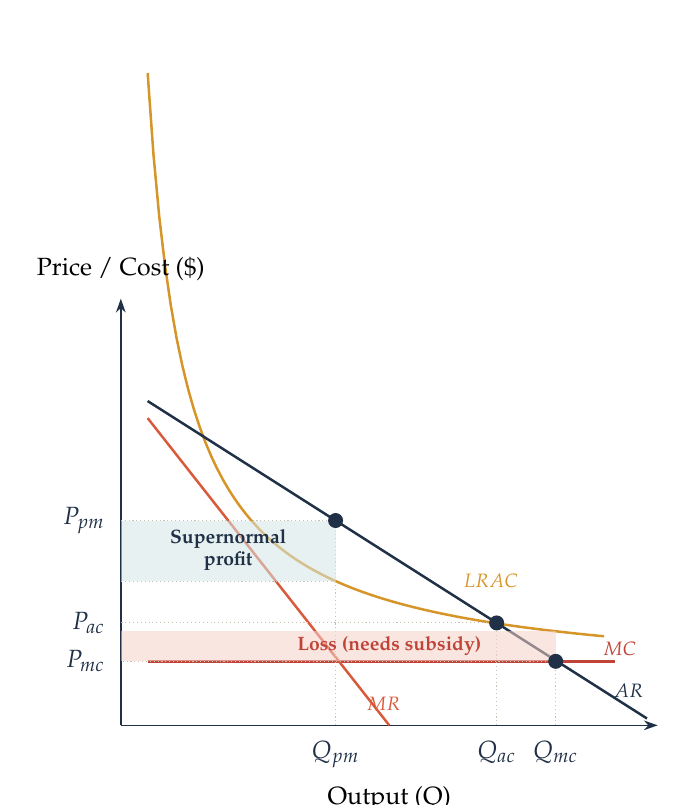
\begin{tikzpicture}[baseline=(current bounding box.center)]
  \begin{axis}[econ chart,
    width=8.4cm, height=7.0cm,
    xmin=0, xmax=100, ymin=0, ymax=100,
    xlabel={\small Output (Q)},
    ylabel={\small Price / Cost (\$)},
    xlabel style={at={(ticklabel cs:0.5)}, anchor=north},
    xtick={40,70,81}, xticklabels={$Q_{pm}$,$Q_{ac}$,$Q_{mc}$},
    ytick={15,24,48}, yticklabels={$P_{mc}$,$P_{ac}$,$P_{pm}$}
  ]
    % --- Cost curves ------------------------------------------------
    % LRAC: 1000/(x+2) + 10  (falls throughout: natural monopoly)
    \addplot[curve accent, domain=5:90, samples=80] {1000/(x+2) + 10};
    \node[font=\scriptsize, color=CurveGold, anchor=south west]
        at (axis cs:62,30) {$LRAC$};
    % MC: flat at 15 (constant marginal cost, classic NM assumption)
    \addplot[curve danger, domain=5:92] {15};
    \node[font=\scriptsize, color=CurveDanger, anchor=west]
        at (axis cs:88,18) {$MC$};
    % --- Demand ------------------------------------------------------
    \addplot[curve primary, domain=5:98] {-0.8*x + 80};
    \node[font=\scriptsize\itshape, color=CurveNavy, anchor=west]
        at (axis cs:90,8) {$AR$};
    % MR: half-slope of AR.  Label placed in the clear strip between MR
    % and the x-axis, to the right of the supernormal-profit rectangle.
    \addplot[curve secondary, domain=5:50] {-1.6*x + 80};
    \node[font=\scriptsize\itshape, color=CurveRose, anchor=west]
        at (axis cs:44,5) {$MR$};
    % --- Equilibria --------------------------------------------------
    %  Profit-max:  MR=MC -> Q_pm=40, P_pm=48, LRAC(40)=33.81
    \addplot[guide projection] coordinates {(40,0)(40,48)(0,48)};
    \addplot[guide projection] coordinates {(40,33.81)(0,33.81)};
    %  Average-cost pricing:  Q_ac=70, P_ac≈24
    \addplot[guide projection] coordinates {(70,0)(70,24)(0,24)};
    %  Marginal-cost pricing: Q_mc=81, P_mc=15 (= MC)
    \addplot[guide projection] coordinates {(81,0)(81,15)(0,15)};
    \addplot[only marks, mark=*, mark size=2.5pt, color=AxisCharcoal]
        coordinates {(40,48)(70,24)(81,15)};
    % --- Supernormal-profit rectangle (at profit-max) ---------------
    \fill[FillPrimary, opacity=0.55]
        (axis cs:0,33.81) rectangle (axis cs:40,48);
    \node[font=\scriptsize\bfseries, color=CurveNavy, align=center]
        at (axis cs:20,41) {Supernormal\\profit};
    % --- Loss rectangle (at MC-pricing) -----------------------------
    \fill[FillNegative, opacity=0.55]
        (axis cs:0,15) rectangle (axis cs:81,22);
    \node[font=\scriptsize\bfseries, color=CurveDanger, align=center]
        at (axis cs:50,18.5) {Loss (needs subsidy)};
  \end{axis}
\end{tikzpicture}%
}{%
\textbf{\color{CurveNavy}The falling-LRAC dilemma:} for a natural monopoly, one firm is always cheaper than two.\\[5pt]
$\bullet$\enspace \textit{Profit-max}: produces little ($Q_{pm}$), charges high price $P_{pm}$, earns the blue rectangle of supernormal profit.\\[2pt]
$\bullet$\enspace \textit{Average-cost pricing}: regulator sets $P_{ac}=LRAC$, expanding output to $Q_{ac}$ with only normal profit.\\[2pt]
$\bullet$\enspace \textit{Marginal-cost pricing}: $P=MC$ is allocatively efficient at $Q_{mc}$, but $P<LRAC$ -- the firm makes a loss (red rectangle) and needs a subsidy.%
}
\end{diagrambox}

\begin{diagrambox}[Monopolistic Competition -- Short Run and Long Run]
\tworowwithtext{%
% --- Short Run -----------------------------------------------------
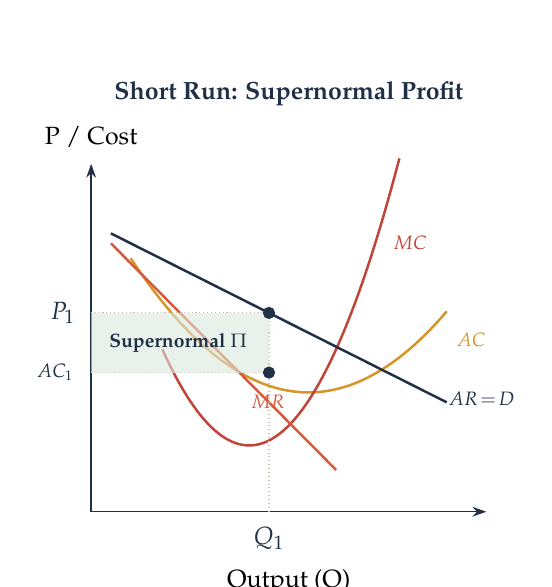
\begin{tikzpicture}[baseline=(current bounding box.center)]
  \begin{axis}[econ chart,
    width=6.6cm, height=6.0cm,
    xmin=0, xmax=100, ymin=0, ymax=105,
    xlabel={\small Output (Q)},
    ylabel={\small P / Cost},
    xlabel style={at={(ticklabel cs:0.5)}, anchor=north},
    xtick={45}, xticklabels={$Q_1$},
    ytick={60}, yticklabels={$P_1$},
    title={\small\bfseries\color{CurveNavy} Short Run: Supernormal Profit},
    title style={at={(0.5,1.06)}, anchor=south, yshift=4pt}
  ]
    % AC — gold U-shape
    \addplot[curve accent, domain=10:90, samples=60] {0.02*(x-55)^2 + 36};
    \node[font=\scriptsize, color=CurveGold, anchor=west] at (axis cs:90,52) {$AC$};
    % MC — red, crosses AC at AC's minimum (x=55)
    \addplot[curve danger, domain=18:78, samples=60] {0.06*(x-40)^2 + 20};
    \node[font=\scriptsize, color=CurveDanger, anchor=south west] at (axis cs:74,76) {$MC$};
    % AR=D — navy, downward sloping
    \addplot[curve primary, domain=5:90] {-0.6*x + 87};
    \node[font=\scriptsize\itshape, color=CurveNavy, anchor=west] at (axis cs:88,34) {$AR\!=\!D$};
    % MR — rose, twice the slope.
    \addplot[curve secondary, domain=5:62] {-1.2*x + 87};
    \node[font=\scriptsize\itshape, color=CurveRose, anchor=north west] at (axis cs:38,38) {$MR$};
    % Projection lines + equilibrium markers
    \addplot[guide projection] coordinates {(45,0)(45,60)(0,60)};
    \addplot[guide projection] coordinates {(0,42)(45,42)};
    \addplot[only marks, mark=*, mark size=2pt, color=AxisCharcoal] coordinates {(45,60)(45,42)};
    \node[font=\scriptsize, color=AxisCharcoal, anchor=east] at (axis cs:-2,42) {$AC_1$};
    % Profit rectangle
    \fill[FillPositive, opacity=0.6] (axis cs:0,42) rectangle (axis cs:45,60);
    \node[font=\scriptsize\bfseries, color=CurveNavy] at (axis cs:22,51) {Supernormal $\Pi$};
  \end{axis}
\end{tikzpicture}
}{%
% --- Long Run ------------------------------------------------------
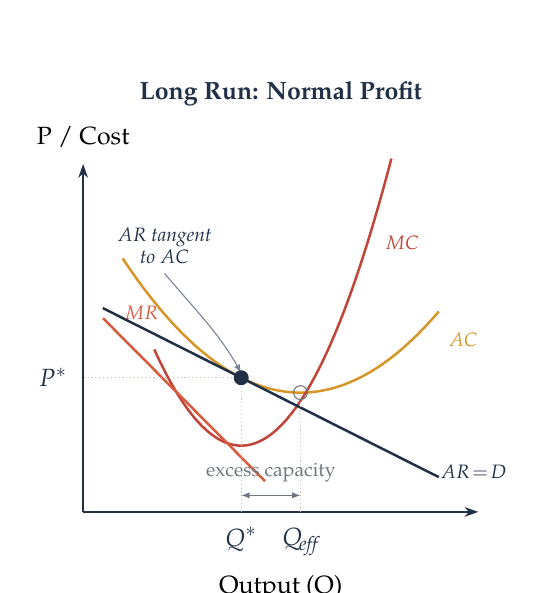
\begin{tikzpicture}[baseline=(current bounding box.center)]
  \begin{axis}[econ chart,
    width=6.6cm, height=6.0cm,
    xmin=0, xmax=100, ymin=0, ymax=105,
    xlabel={\small Output (Q)},
    ylabel={\small P / Cost},
    xlabel style={at={(ticklabel cs:0.5)}, anchor=north},
    xtick={40,55}, xticklabels={$Q^*$,$Q_{\!\textit{eff}}$},
    ytick={40.5}, yticklabels={$P^*$},
    title={\small\bfseries\color{CurveNavy} Long Run: Normal Profit},
    title style={at={(0.5,1.06)}, anchor=south, yshift=4pt}
  ]
    % Same cost curves
    \addplot[curve accent, domain=10:90, samples=60] {0.02*(x-55)^2 + 36};
    \node[font=\scriptsize, color=CurveGold, anchor=west] at (axis cs:90,52) {$AC$};
    \addplot[curve danger, domain=18:78, samples=60] {0.06*(x-40)^2 + 20};
    \node[font=\scriptsize, color=CurveDanger, anchor=south west] at (axis cs:74,76) {$MC$};
    % AR shifted left, tangent to AC at (40, 40.5).
    % AC'(40) = 0.04*(40-55) = -0.6, so AR has slope -0.6.
    % AR(40) = AC(40) = 0.02*225 + 36 = 40.5  =>  AR(x) = -0.6x + 64.5
    \addplot[curve primary, domain=5:90] {-0.6*x + 64.5};
    \node[font=\scriptsize\itshape, color=CurveNavy, anchor=west] at (axis cs:88,12) {$AR\!=\!D$};
    % MR — label placed top-left of the dashed curve so it can't collide
    % with the "excess capacity" double arrow at the bottom.
    \addplot[curve secondary, domain=5:46] {-1.2*x + 64.5};
    \node[font=\scriptsize\itshape, color=CurveRose, anchor=south west] at (axis cs:8,55) {$MR$};
    % Equilibrium markers
    \addplot[guide projection] coordinates {(40,0)(40,40.5)(0,40.5)};
    \addplot[only marks, mark=*, mark size=2.5pt, color=CurveNavy] coordinates {(40,40.5)};
    % Q_eff marker (= AC min)
    \addplot[guide projection] coordinates {(55,0)(55,36)};
    \addplot[only marks, mark=o, mark size=2.5pt, color=AnnotGray] coordinates {(55,36)};
    % Excess-capacity arrow — between Q* and Q_eff at low y so it clears
    % the MR curve and the x-axis label.
    \draw[{Latex[length=3pt]}-{Latex[length=3pt]}, color=AnnotGray,
          line width=0.4pt]
      (axis cs:40,5) -- (axis cs:55,5);
    \node[font=\scriptsize, color=AnnotGray, anchor=south]
      at (axis cs:47.5,6) {excess capacity};
    % Tangency callout — pushed up to clear the AC curve, with a short
    % leader pointing into the equilibrium dot.
    \node[font=\scriptsize\itshape, color=CurveNavy, align=center,
          anchor=south east] (tantxt) at (axis cs:35,72)
      {$AR$ tangent\\to $AC$};
    \draw[-{Latex[length=3pt]}, color=CurveNavy!60, line width=0.4pt]
      (tantxt.south) to[out=-50, in=120] (axis cs:40,42);
  \end{axis}
\end{tikzpicture}%
}{%
\textbf{\color{CurveNavy}Short Run:} the firm uses its product differentiation to set price above marginal cost.  At the profit-max output $Q_1$ (where $MR=MC$), price $P_1$ exceeds $AC_1$, so the firm earns \textit{supernormal profit} (shaded green).\quad
\textbf{\color{CurveNavy}Long Run:} supernormal profit attracts new entrants.  Each existing firm's demand shifts left and becomes more elastic until $AR$ is just \textit{tangent} to $AC$ at $Q^*$.  Profit is exactly normal ($P^*\!=\!AC$).  Because the tangency lies to the left of the AC minimum, the firm operates with \textbf{excess capacity} ($Q^*<Q_{\textit{eff}}$) -- the hallmark inefficiency of monopolistic competition.%
}
\end{diagrambox}


\begin{diagrambox}[Oligopoly -- Kinked Demand Curve (Price Rigidity)]
\diagramwithtext{%
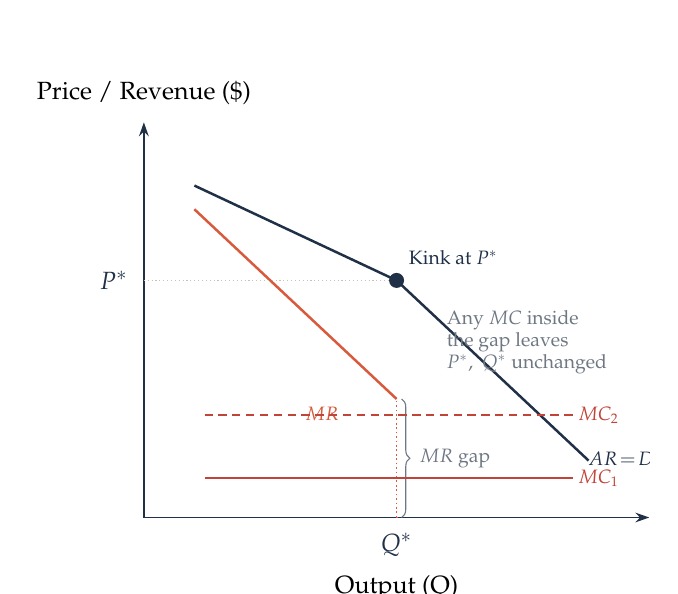
\begin{tikzpicture}[baseline=(current bounding box.center)]
  \begin{axis}[econ chart,
    clip=true,
    width=8.0cm, height=6.6cm,
    xmin=0, xmax=100, ymin=0, ymax=100,
    xlabel={\small Output (Q)},
    ylabel={\small Price / Revenue (\$)},
    xlabel style={at={(ticklabel cs:0.5)}, anchor=north},
    xtick={50}, xticklabels={$Q^*$},
    ytick={60}, yticklabels={$P^*$}
  ]
    % --- Kinked demand (AR=D) -------------------------------------
    % Upper (elastic) segment: slope -0.6, through (50,60) -> P = -0.6Q + 90
    \addplot[curve primary, domain=10:50] {-0.6*x + 90};
    % Lower (inelastic) segment: slope -1.2, through (50,60) -> P = -1.2Q + 120
    \addplot[curve primary, domain=50:88] {-1.2*x + 120};
    \node[font=\scriptsize\itshape, color=CurveNavy, anchor=west]
        at (axis cs:86,15) {$AR\!=\!D$};

    % Kink marker
    \addplot[only marks, mark=*, mark size=2.5pt, color=CurveNavy]
        coordinates {(50,60)};
    \node[font=\scriptsize, color=CurveNavy, anchor=south west]
        at (axis cs:50.5,61.5) {Kink at $P^*$};

    % --- Marginal-revenue curve (MR) ------------------------------
    % Upper MR (from elastic AR): slope -1.2, MR = -1.2Q + 90.
    % At Q=50, MR=30 (top of the gap).
    \addplot[curve secondary, domain=10:50] {-1.2*x + 90};
    % Lower MR (from inelastic AR): MR = -2.4Q + 120, but this drops below
    % the axis instantly.  Draw just a short stub from (50,0) going down-right
    % to indicate where the lower MR would continue.
    \addplot[curve secondary, domain=50:51, samples=2] {-2.4*x + 120};
    \node[font=\scriptsize\itshape, color=CurveRose, anchor=south west]
        at (axis cs:30,22) {$MR$};

    % MR-gap segment (the vertical discontinuity at Q*)
    \draw[densely dotted, color=CurveRose, line width=0.6pt]
        (axis cs:50,0) -- (axis cs:50,30);
    \draw[decorate, decoration={brace, amplitude=3pt}, color=AnnotGray,
          line width=0.4pt]
        (axis cs:51,30) -- (axis cs:51,0)
        node[midway, right=3pt, font=\scriptsize, color=AnnotGray]
        {$MR$ gap};

    % --- MC curves (any MC in the gap yields the same Q*, P*) -----
    \addplot[curve danger, domain=12:85] {10};
    \node[font=\scriptsize, color=CurveDanger, anchor=west]
        at (axis cs:84,10) {$MC_1$};
    \addplot[curve danger, densely dashed, domain=12:85] {26};
    \node[font=\scriptsize, color=CurveDanger, anchor=west]
        at (axis cs:84,26) {$MC_2$};

    % Q* projection (only the horizontal from y-axis to the kink)
    \addplot[guide projection] coordinates {(0,60)(50,60)};

    % Explanatory callout near the gap
    \node[font=\scriptsize, color=AnnotGray, align=left, anchor=north west]
        at (axis cs:58,55)
        {Any $MC$ inside\\the gap leaves\\$P^*,\;Q^*$ unchanged};
  \end{axis}
\end{tikzpicture}%
}{%
\textbf{\color{CurveNavy}Price rigidity:} the upper (elastic) section of the demand curve reflects the assumption that \textit{rivals don't match price rises} -- so a price increase loses customers fast.  The lower (inelastic) section reflects rivals \textit{matching price cuts} -- so a price cut wins few extra customers.\\[5pt]
The resulting kink at $P^*$ creates a \textbf{discontinuity in $MR$}: it jumps down from \$30 to \$0 at $Q^*$.  Any marginal-cost curve passing through this gap delivers the same profit-maximising $Q^*$ -- explaining why oligopoly prices stay sticky even as costs change.%
}
\end{diagrambox}

\subsection{Concentration Ratio}

\begin{keyterm}{Concentration Ratio}
A measure of the total market share held by the largest `n' firms in an industry. For example, the 3-firm concentration ratio (CR3) or the 5-firm ratio (CR5).
\[ CR_3 = \text{Market share of firm 1} + \text{firm 2} + \text{firm 3} \]
If the top 3 firms have market shares of 30\%, 25\%, and 15\%, then CR3 = 70\%.
\end{keyterm}

Relationship to market structures: Perfect Competition has a very low CR (e.g., $<$20\%); Oligopoly has a high CR (e.g., CR4 $>$ 60\% is a typical indicator); Monopoly has CR1 = 100\%.

\begin{evaluation}{Perfect Competition vs. Monopoly (Efficiency Comparison)}
\textbf{Strengths / Arguments For Perfect Competition:}
\begin{itemize}[leftmargin=*, nosep]
\item Allocatively efficient: $P = MC$, no deadweight loss, consumer and producer surplus maximised in total.
\item Productively efficient in long run: firms operate at minimum AC, no excess capacity.
\item Dynamic efficiency: firms must innovate and cut costs to survive; weak firms exit.
\item Consumer surplus maximised; prices are low and variety reflects actual demand.
\end{itemize}
\textbf{Strengths / Arguments For Monopoly:}
\begin{itemize}[leftmargin=*, nosep]
\item Can exploit economies of scale; larger firm = lower AC per unit (natural monopoly).
\item High profits can fund R\&D and innovation; monopoly may generate dynamic efficiency gains.
\item Marketing and brand investment create consumer trust and quality signals.
\item Barriers to entry can protect investment in innovation (e.g., patents incentivise drug development).
\end{itemize}
\textbf{Limitations / Arguments Against Perfect Competition:}
\begin{itemize}[leftmargin=*, nosep]
\item Zero profit in long run reduces incentive for risky R\&D; may lead to static efficiency.
\item Atomistic competition makes it hard to achieve scale economies; duplication of fixed costs.
\item Information asymmetries in real markets mean consumers don't always behave as theory predicts.
\end{itemize}
\textbf{Limitations / Arguments Against Monopoly:}
\begin{itemize}[leftmargin=*, nosep]
\item Allocatively inefficient: $P > MC$ creates deadweight loss; consumer surplus transferred to producer.
\item Productive inefficiency: no competitive pressure, X-inefficiency (lazy management, high costs).
\item Lock-in effects trap consumers; lack of innovation if profits don't depend on it.
\item Market power can be abused: predatory pricing, excessive pricing, quality shrinkflation.
\end{itemize}
\textbf{It depends on\ldots}
\begin{itemize}[leftmargin=*, nosep]
\item The size of economies of scale: large scale economies justify monopoly; none justify competition.
\item The pace of technological change: innovation-heavy industries may need monopoly rents; static goods benefit from competition.
\item Contestability of the market: even a monopoly can be efficient if entry threats are credible.
\item Regulatory environment: can monopoly be regulated to mimic competitive outcomes?
\end{itemize}
\end{evaluation}

\begin{evaluation}{Monopolistic Competition (Allocative vs. Productive Efficiency)}
\textbf{Strengths / Arguments For Monopolistic Competition:}
\begin{itemize}[leftmargin=*, nosep]
\item Product differentiation creates consumer choice and variety; consumers value this.
\item Low barriers to entry ensure contestability; supernormal profit attracts entry and competes them away (LR).
\item Long-run normal profit is consistent with fair returns and a competitive industry.
\item Combines some monopoly power (allows investment) with competitive discipline (entry threat).
\end{itemize}
\textbf{Limitations / Efficiency Problems:}
\begin{itemize}[leftmargin=*, nosep]
\item Allocatively inefficient in long run: $P > MC$, though by less than monopoly.
\item Productively inefficient: operates with excess capacity (left of min AC) due to downward-sloping demand.
\item Wasteful advertising and non-price competition; firms spend to steal market share rather than reduce costs.
\item Mark-up over MC may not be justified by genuine product quality differences; artificial differentiation.
\end{itemize}
\textbf{Counterarguments to Efficiency Critique:}
\begin{itemize}[leftmargin=*, nosep]
\item Product variety has real value to consumers; static efficiency analysis ignores this benefit.
\item Excess capacity is not `waste' if it funds innovation and design; trade-off between choice and efficiency.
\item Advertising provides information and builds trust; not always wasteful.
\end{itemize}
\textbf{It depends on\ldots}
\begin{itemize}[leftmargin=*, nosep]
\item The degree of product differentiation: genuine functional differences justify premium; cosmetic changes do not.
\item Consumer preferences: if variety is highly valued (e.g., restaurants), loss of static efficiency is acceptable.
\item Contestability: rapid entry discipline keeps excess capacity small.
\end{itemize}
\end{evaluation}

\begin{evaluation}{Oligopoly and Game Theory (Collusion vs. Competition)}
\textbf{Strengths / Arguments For Cartelisation / Collusion:}
\begin{itemize}[leftmargin=*, nosep]
\item Firms can reach more profitable equilibrium (like monopoly) if they cooperate.
\item Reduced price competition lowers uncertainty and investment risk.
\item Can fund long-term R\&D with sustained high profits (e.g., OPEC R\&D in renewable alternatives).
\end{itemize}
\textbf{Limitations / Why Cartels Collapse (Prisoners' Dilemma):}
\begin{itemize}[leftmargin=*, nosep]
\item Each firm has incentive to cheat: secret price cuts gain market share while cartel price holds up.
\item Enforcement is difficult if firms are geographically dispersed or information is asymmetric.
\item Cartel profits attract entry (unless barriers are very high); new firms break the agreement.
\item Legal risk: cartels are illegal in most jurisdictions (competition law); detection risk rises over time.
\end{itemize}
\textbf{Strengths / Arguments For Competitive Oligopoly:}
\begin{itemize}[leftmargin=*, nosep]
\item Price wars and innovation benefit consumers (e.g., supermarkets, airlines).
\item Kinked demand curve explains price stickiness without collusion; natural equilibrium.
\item Dynamic competition can be fierce; firms race to innovate and cut costs.
\end{itemize}
\textbf{It depends on\ldots}
\begin{itemize}[leftmargin=*, nosep]
\item Number and symmetry of firms: fewer firms and similar costs make collusion easier.
\item Product homogeneity: identical products tempt price competition; differentiation helps collusion.
\item Barriers to entry: high barriers protect cartels; low barriers destroy them via entry.
\item Transparency of pricing: if prices are public and easy to monitor, collusion is easier (e.g., petrol prices).
\item Legal enforcement: weak anti-trust enforcement tempts collusion; strong enforcement prevents it.
\end{itemize}
\end{evaluation}

\begin{evaluation}{Price Discrimination (Welfare Effects and Fairness)}
\textbf{Strengths / Arguments For Price Discrimination:}
\begin{itemize}[leftmargin=*, nosep]
\item Increases firm profits and incentives for investment and innovation; more supernormal profit funds R\&D.
\item Can increase total output compared to single-price monopoly (2nd-degree discrimination); allocatively more efficient.
\item Allows low-income consumers to buy (student discounts, off-peak pricing) who would be priced out otherwise.
\item Encourages firms to serve heterogeneous markets (geographic, demographic); increases coverage and choice.
\end{itemize}
\textbf{Limitations / Fairness and Efficiency Concerns:}
\begin{itemize}[leftmargin=*, nosep]
\item Creates inequality: consumers with inelastic demand (e.g., poor health patients) pay higher prices.
\item Deadweight loss still exists if not all consumers at MC-willing price are served.
\item Creates perverse incentives for cost-shifting and arbitrage (grey markets, parallel importing).
\item First-degree discrimination (perfect) extracts all consumer surplus; maximally unfair to consumers.
\item Information barriers may not reflect ability-to-pay but arbitrary group membership (e.g., age, gender).
\end{itemize}
\textbf{Empirical Reality:}
\begin{itemize}[leftmargin=*, nosep]
\item 3rd-degree (market segmentation) most common and defensible: student discounts are based on lower willingness-to-pay.
\item 2nd-degree (quantity/quality tiers) generally welfare-improving: forces self-selection by willingness-to-pay.
\item 1st-degree rare and ethically contentious: airlines approaching it with personalised pricing.
\end{itemize}
\textbf{It depends on\ldots}
\begin{itemize}[leftmargin=*, nosep]
\item The degree of discrimination: small differences are acceptable; large gaps raise fairness concerns.
\item The basis for discrimination: cost-based discrimination (e.g., shipping cost differences) is fairer than pure rent extraction.
\item Information availability: can consumers find the best price, or does opacity trap them?
\item Regulation: some jurisdictions cap price discrimination (e.g., insurance must use objective risk factors).
\end{itemize}
\end{evaluation}

\begin{evaluation}{Natural Monopoly and Regulation}
\textbf{Strengths / Arguments For Leaving Unregulated:}
\begin{itemize}[leftmargin=*, nosep]
\item Single firm produces at lowest AC; competition would duplicate fixed costs (railways, utilities).
\item Profit motive funds investment in network infrastructure (broadband, electricity grids).
\item Unregulated firm can achieve dynamic efficiency through innovation (e.g., new technologies).
\end{itemize}
\textbf{Strengths / Arguments For Regulation:}
\begin{itemize}[leftmargin=*, nosep]
\item Unregulated monopoly sets $P > ATC$, earning supernormal profit and deadweight loss.
\item Essential services (water, electricity) should not be profit-maximised; exploit captive consumers.
\item Network effects mean entry is impossible; regulation is only check on monopoly power.
\end{itemize}
\textbf{Regulatory Options (Trade-offs):}
\begin{itemize}[leftmargin=*, nosep]
\item \textbf{Price controls (P = MC):} Allocatively efficient but firm may not break even; requires subsidy, political risk.
\item \textbf{Price controls (P = AC):} Firm breaks even, normal profit only; incentive for efficiency reduced, bureaucratic costs.
\item \textbf{Nationalisation:} Government operates; accountability but potential for political interference and inefficiency.
\item \textbf{Competition / break-up:} Duplication of fixed costs eliminates efficiency gains (e.g., two railway networks).
\item \textbf{Franchising:} Auction monopoly rights, firm keeps profit but must compete for the franchise; balances efficiency with competition.
\end{itemize}
\textbf{It depends on\ldots}
\begin{itemize}[leftmargin=*, nosep]
\item The source of the monopoly: true natural monopoly (declining AC) vs. temporary monopoly (patents).
\item Technological change: advances may erode the natural monopoly (e.g., broadband competes with telephony).
\item Quality of regulation: can government commit to stable rules and avoid capture by the regulated firm?
\item Alternative funding: can network be funded by tax (public good view) or must user pay?
\end{itemize}
\end{evaluation}

\begin{evaluation}{Contestable Markets and Efficiency}
\textbf{Strengths / Arguments For Contestability:}
\begin{itemize}[leftmargin=*, nosep]
\item Even monopolies behave competitively if entry is costless and quick (hit-and-run entry threat).
\item More realist than perfect competition: explains pricing in real concentrated markets (e.g., airlines on routes).
\item Eliminates need to count firms; focus on barriers to entry instead (more useful policy guide).
\item Predicts allocative efficiency even with few firms if contestability holds.
\end{itemize}
\textbf{Limitations / Realism Check:}
\begin{itemize}[leftmargin=*, nosep]
\item Sunk costs are real: most markets have setup costs (R\&D, advertising, retooling) that cannot be recovered.
\item Hit-and-run entry rare in practice: firms must operate long enough to recover sunk costs, so threat is weak.
\item Incumbent firm has cost advantage (scale, experience, brand); entrant must be very efficient to undercut.
\item Predatory actions (limit pricing, exclusive contracts) deter entry more than theory predicts.
\end{itemize}
\textbf{Empirical Support:}
\begin{itemize}[leftmargin=*, nosep]
\item Airlines on less popular routes do show competitive pricing despite duopoly/monopoly structure (some sunk costs are flight-specific, not airport-specific).
\item But in infrastructure (railways, telecommunications), high sunk costs mean contestability is weak; regulation needed.
\end{itemize}
\textbf{It depends on\ldots}
\begin{itemize}[leftmargin=*, nosep]
\item The size of sunk costs relative to profit: if sunk costs exceed potential profit, no entry threat.
\item Technology and time horizons: fast-moving tech (software) more contestable than slow infrastructure (railways).
\item Regulatory environment: entry regulations (licenses, permits) are artificial barriers; remove them to increase contestability.
\end{itemize}
\end{evaluation}

% ─────────────────────────────────────────────────────────────
\section{Growth and Survival of Firms}

\subsection{Reasons for Different Sizes of Firms}

\textbf{Why Most Firms Remain Small:}
\begin{itemize}
  \item \textbf{Market Size \& Niche Markets:} The total demand for the product/service is limited (e.g., a local artisan bakery, an independent hair salon).
  \item \textbf{Owner Objectives:} Many owners prioritise independence, work-life balance, or a passion project over profit/growth maximisation. They are ``satisficers''.
  \item \textbf{Barriers to Growth:} Lack of access to finance (capital), skilled labour, or managerial expertise can trap firms.
  \item \textbf{Diseconomies of Scale:} For some businesses, growing larger leads to increased average costs due to poor communication, coordination issues, and low morale.
  \item \textbf{Market Nature:} Some industries are inherently fragmented and localised (e.g., cafes, tradespeople, boutique retail).
\end{itemize}

\textbf{Why Some Firms Experience Growth:}
\begin{itemize}
  \item \textbf{Profit Motive:} The primary driver. Growth can lead to economies of scale (lower LRAC), higher market share, and greater profit.
  \item \textbf{Market Power:} Larger firms can influence prices (price makers), deter new entrants, and secure better deals from suppliers.
  \item \textbf{Diversification of Risk:} Growing into new markets or products spreads risk (``not putting all your eggs in one basket'').
  \item \textbf{Managerial Motives:} Managers may seek growth for higher salaries, prestige, and power (linked to the principal-agent problem).
\end{itemize}

\subsection{Internal Growth of Firms (Organic Growth)}

\begin{keyterm}{Organic Growth}
Growth generated from within the firm using its own resources: investing in new capital/technology; developing new products (R\&D); increasing marketing efforts; opening new locations. Less risky and less disruptive than mergers, and it maintains the firm's own culture and management control.
\end{keyterm}

\begin{keyterm}{Economies of Scope}
The cost advantage achieved when a firm produces a \textbf{variety of products} rather than specialising. The cost of producing two (or more) products jointly is less than producing them separately (e.g., a supermarket selling bread and milk shares storage, checkout, and marketing costs). This is the key concept behind diversification.
\end{keyterm}

\subsection{External Growth -- Integration (Mergers \& Takeovers)}

\begin{keyterm}{Horizontal Integration}
A merger between firms at the \textbf{same stage of production} in the same industry (e.g., two car manufacturers merging, two supermarkets merging). Aim: to instantly increase market share, reduce competition, and achieve economies of scale.
\end{keyterm}

\begin{keyterm}{Vertical Integration}
A merger between firms at \textbf{different stages of production} in the same industry. \textbf{Backwards:} merging with a supplier (e.g., a car maker buys a tyre company) to gain control of inputs. \textbf{Forwards:} merging with a distributor/retailer (e.g., a car maker buys a chain of showrooms) to gain control of output.
\end{keyterm}

\begin{keyterm}{Conglomerate Integration}
A merger between firms in \textbf{completely unrelated industries} (e.g., a tobacco company buying a food brand). Purely for diversification and risk spreading.
\end{keyterm}

\textbf{Consequences of Integration:}
\begin{itemize}
  \item \textbf{For Firms:} Potential for lower costs, higher profits, increased market power. Risk of over-extension, culture clashes, and regulatory opposition.
  \item \textbf{For Consumers:} Potential negatives: less choice and higher prices (reduced competition). Potential positives: lower prices if cost savings are passed on, better quality from improved coordination.
  \item \textbf{For Workers:} Could lead to job losses due to rationalisation (especially in horizontal mergers). Possible job security from being part of a larger, more stable firm.
\end{itemize}

\subsection{Cartels}

\begin{keyterm}{Cartel}
A formal agreement between independent firms in an oligopolistic market to collude -- fix prices, limit output, and carve up markets. The aim is to act collectively as a monopoly.
\end{keyterm}

\textbf{Conditions for an Effective Cartel:}
\begin{itemize}
  \item Small number of dominant firms (easier to monitor and agree).
  \item High barriers to entry (to prevent firms undercutting the cartel price from outside).
  \item Similar costs and products (makes agreement on price and output easier).
  \item Ability to detect and punish cheating -- if one firm secretly lowers its price to gain market share, the cartel collapses.
\end{itemize}

\textbf{Consequences:}
\begin{itemize}
  \item \textbf{Allocative Inefficiency:} Higher prices (P $>$ MC) and lower output than in a competitive market.
  \item \textbf{Reduced Consumer Surplus:} Welfare is transferred from consumers to producers.
  \item \textbf{Productive Inefficiency:} Lack of competitive pressure can lead to X-inefficiency (firms become lazy and costs rise).
  \item \textbf{From the firms' perspective:} Guaranteed supernormal profits and price stability, which could in theory fund R\&D.
\end{itemize}

\subsection{Principal-Agent Problem}

\begin{keyterm}{Principal-Agent Problem}
A conflict in priorities between the \textbf{owners} of a firm (the principals, e.g., shareholders) and those \textbf{hired to run it} (the agents, e.g., managers). It arises because of differing objectives and asymmetric information.
\end{keyterm}

\begin{itemize}
  \item \textbf{Differing Objectives:} Shareholders primarily want maximised shareholder value (profits, dividends, share price). Managers may want maximised salaries, job perks, prestige, power, and job security -- often achieved by growing the firm's size (sales, market share) rather than its profitability.
  \item \textbf{Asymmetric Information:} Managers (agents) have more information about day-to-day operations, costs, and opportunities than the distant shareholders (principals). This information gap allows managers to pursue their own goals without shareholders easily detecting it (e.g., overspending on lavish offices, making poor acquisitions for empire-building).
  \item \textbf{Consequences:} The firm may not be profit-maximising. It leads to a \textbf{divorce of ownership from control}.
  \item \textbf{Solutions to Align Interests:} Performance-related pay for managers (share options, bonuses), threat of takeover (poorly run firms become targets), appointing non-executive directors to monitor management.
\end{itemize}

% ─────────────────────────────────────────────────────────────
\section{Differing Objectives and Policies of Firms}

\subsection{Traditional Profit Maximisation Objective}

\begin{keyterm}{Profit Maximisation}
The condition: firms maximise profit where \textbf{Marginal Cost (MC) = Marginal Revenue (MR)}. If MR $>$ MC, producing one more unit adds more to revenue than to cost, so profit increases. If MR $<$ MC, that last unit cost more than it earned, reducing profit. Therefore, profit is maximised only when MC = MR.
\end{keyterm}

\textbf{Why Firms Might NOT Operate at This Level:}
\begin{itemize}
  \item \textbf{Lack of Information:} Firms may not know their exact MC and MR curves in reality.
  \item \textbf{Other Objectives:} They may prioritise growth, market share, or simply satisfactory profit.
  \item \textbf{Behavioural Theories:} Managers (agents) may run the firm to maximise their own utility (big offices, perks) rather than the owners' (shareholders') profits.
  \item \textbf{Short-Term vs.\ Long-Term:} Sacrificing maximum profit now (e.g., by investing in R\&D or lowering prices to deter competitors) can lead to greater long-term profits.
\end{itemize}

\subsection{Other Objectives of Firms}

Firms have a variety of goals, especially in large corporations where ownership (shareholders) is separate from control (managers).

\begin{itemize}
  \item \textbf{Survival:} The most fundamental objective, especially for new firms or during a recession. Prices may be set very low just to cover variable costs and stay in the market.
  \item \textbf{Profit Satisficing:} Instead of maximising profit, managers aim for a ``satisfactory'' level of profit that keeps shareholders content, then pursue other goals (sales growth, market share, a quiet life). It's a compromise.
  \item \textbf{Sales Maximisation:} Aiming to sell as much output as possible without making a loss. The firm produces where AR = AC (TR = TC), meaning only normal profit is made. Often used to gain market dominance.
  \item \textbf{Revenue Maximisation:} Aiming to maximise total sales revenue. The firm produces where MR = 0. Producing any further would make MR negative and reduce total revenue. Often linked to managerial prestige or market share.
  \item \textbf{Behavioural Objectives:} Managerial utility (salary, perks, power), ethical goals, corporate social responsibility (CSR), or providing a good service.
\end{itemize}

\begin{coreidea}
\textbf{Order of Output Levels:} For a typical downward-sloping demand curve: Profit Maximisation (MC = MR) $<$ Revenue Maximisation (MR = 0) $<$ Sales Maximisation (AR = AC). Profit-maximising output is the smallest; sales-maximising output is the largest.
\end{coreidea}

\subsection{Price Discrimination}

\begin{keyterm}{Price Discrimination}
Selling the same product/service to different consumers at \textbf{different prices for reasons not associated with costs}.
\end{keyterm}

\textbf{Conditions for Effective Price Discrimination:}
\begin{itemize}
  \item \textbf{Price-Setting Power:} The firm must be a price maker (e.g., a monopoly).
  \item \textbf{Identifiable and Separable Market Segments:} The firm must identify groups with different Price Elasticities of Demand (PED) (e.g., students vs.\ adults, time of travel).
  \item \textbf{Prevention of Resale/Arbitrage:} Consumers from the low-price segment must not be able to resell the product to the high-price segment (e.g., you can't resell a haircut).
\end{itemize}

\textbf{Degrees of Price Discrimination:}
\begin{itemize}
  \item \textbf{First Degree (Perfect):} Charging each consumer the maximum price they are willing to pay (e.g., haggling at a car boot sale). Extracts all consumer surplus.
  \item \textbf{Second Degree:} Prices vary according to the quantity consumed or the version of the product (e.g., bulk-buy discounts, ``economy'' vs.\ ``premium'' software versions).
  \item \textbf{Third Degree:} Charging different prices to different consumer groups based on their PED (e.g., railcards, cinema tickets for seniors/children, peak vs.\ off-peak pricing).
\end{itemize}

\textbf{Consequences:}
\begin{itemize}
  \item \textbf{For Producers:} Can increase supernormal profits. May allow them to cover fixed costs and operate in markets that would otherwise be unprofitable (e.g., a rural bus service).
  \item \textbf{For Consumers -- Mixed:} Those in the inelastic segment (e.g., business travellers) pay higher prices and lose consumer surplus. Those in the elastic segment (e.g., students) may gain access to a good/service they otherwise couldn't afford.
  \item \textbf{For Efficiency:} Can lead to increased output compared to a single-price monopoly, potentially reducing allocative inefficiency. However, it is inequitable (unfair).
\end{itemize}


\begin{diagrambox}[Third-Degree Price Discrimination -- Combined Market]
\diagramwithtext{%
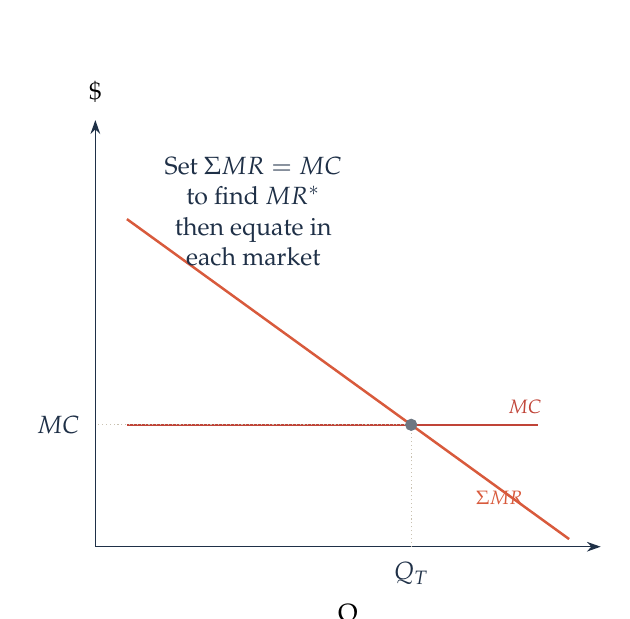
\begin{tikzpicture}[scale=1.0, baseline=(current bounding box.center)]
  \begin{axis}[econ chart,
    xlabel style={at={(ticklabel cs:0.5)}, anchor=north},
    width=8.0cm, height=7.0cm,
    xmin=0, xmax=80, ymin=0, ymax=70,
    xlabel={\small Q}, ylabel={\small \$},
    xtick={50}, xticklabels={$Q_T$},
    ytick={20}, yticklabels={$MC$}
  ]
    \addplot[curve secondary, domain=5:75, samples=60] {-0.75*x + 57.5};
    \node[font=\scriptsize\itshape, color=CurveRose] at (axis cs:64,8) {$\Sigma MR$};
    \addplot[curve danger, domain=5:70] {20};
    \node[font=\scriptsize, color=CurveDanger] at (axis cs:68,23) {$MC$};
    \addplot[guide projection] coordinates {(50,0)(50,20)(0,20)};
    \addplot[only marks, mark=*, mark size=2pt, AnnotGray] coordinates {(50,20)};
    \node[font=\small, align=center, color=CurveNavy] at (axis cs:25,55)
      {Set $\Sigma MR = MC$\\to find $MR^*$\\then equate in\\each market};
  \end{axis}
\end{tikzpicture}%
}{%
\textbf{\color{NavyPrimary}Reading the diagram:}\\[4pt]
Horizontally sum the sub-market MR curves to get $\Sigma MR$.\\[2pt]
Set $\Sigma MR = MC$: this fixes total output $Q_T$ and the common marginal revenue $MR^*$.\\[2pt]
Carry $MR^*$ back to each sub-market to find its price and quantity.%
}
\end{diagrambox}

\begin{diagrambox}[Third-Degree Price Discrimination -- Market 1 (Less Elastic)]
\diagramwithtext{%
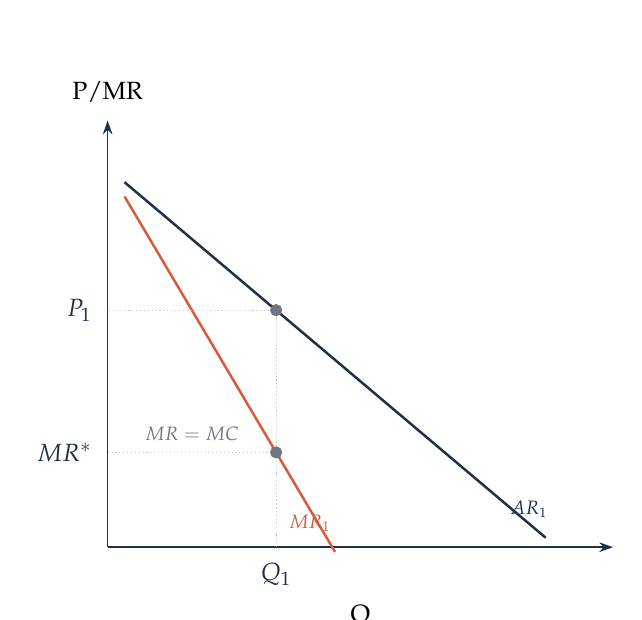
\begin{tikzpicture}[scale=1.0, baseline=(current bounding box.center)]
  \begin{axis}[econ chart,
    xlabel style={at={(ticklabel cs:0.5)}, anchor=north},
    width=8.0cm, height=7.0cm,
    xmin=0, xmax=60, ymin=0, ymax=90,
    xlabel={\small Q}, ylabel={\small P/MR},
    xtick={20}, xticklabels={$Q_1$},
    ytick={20,50}, yticklabels={$MR^*$,$P_1$}
  ]
    \addplot[curve primary, domain=2:52] {-1.5*x + 80};
    \node[font=\scriptsize\itshape, color=CurveNavy] at (axis cs:50,8) {$AR_1$};
    \addplot[curve secondary, domain=2:27] {-3*x + 80};
    \node[font=\scriptsize\itshape, color=CurveRose] at (axis cs:24,5) {$MR_1$};
    \addplot[guide projection] coordinates {(20,0)(20,50)(0,50)};
    \addplot[guide projection] coordinates {(0,20)(20,20)};
    \node[font=\scriptsize, color=AnnotGray] at (axis cs:10,24) {$MR=MC$};
    \addplot[only marks, mark=*, mark size=2pt, AnnotGray] coordinates {(20,50)(20,20)};
  \end{axis}
\end{tikzpicture}%
}{%
\textbf{\color{NavyPrimary}Reading the diagram:}\\[4pt]
In the less-elastic segment, $AR_1$ is steep.\\[2pt]
Imposing $MR_1 = MR^*$ fixes quantity $Q_1$.\\[2pt]
The point on $AR_1$ above $Q_1$ gives price $P_1$, which is relatively high.\\[2pt]
Price-insensitive buyers pay more.%
}
\end{diagrambox}

\begin{diagrambox}[Third-Degree Price Discrimination -- Market 2 (More Elastic)]
\diagramwithtext{%
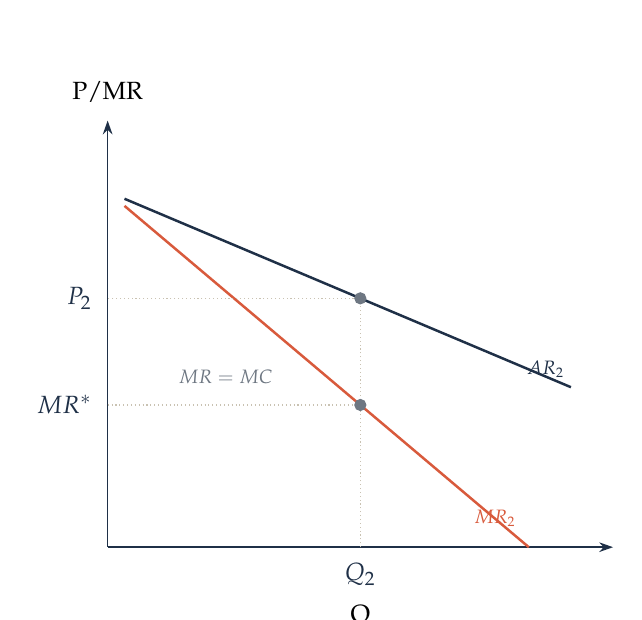
\begin{tikzpicture}[scale=1.0, baseline=(current bounding box.center)]
  \begin{axis}[econ chart,
    xlabel style={at={(ticklabel cs:0.5)}, anchor=north},
    width=8.0cm, height=7.0cm,
    xmin=0, xmax=60, ymin=0, ymax=60,
    xlabel={\small Q}, ylabel={\small P/MR},
    xtick={30}, xticklabels={$Q_2$},
    ytick={20,35}, yticklabels={$MR^*$,$P_2$}
  ]
    \addplot[curve primary, domain=2:55] {-0.5*x + 50};
    \node[font=\scriptsize\itshape, color=CurveNavy] at (axis cs:52,25) {$AR_2$};
    \addplot[curve secondary, domain=2:50] {-x + 50};
    \node[font=\scriptsize\itshape, color=CurveRose] at (axis cs:46,4) {$MR_2$};
    \addplot[guide projection] coordinates {(30,0)(30,35)(0,35)};
    \addplot[guide projection] coordinates {(0,20)(30,20)};
    \node[font=\scriptsize, color=AnnotGray] at (axis cs:14,24) {$MR=MC$};
    \addplot[only marks, mark=*, mark size=2pt, AnnotGray] coordinates {(30,35)(30,20)};
  \end{axis}
\end{tikzpicture}%
}{%
\textbf{\color{NavyPrimary}Reading the diagram:}\\[4pt]
The more-elastic segment has a flatter $AR_2$.\\[2pt]
$MR_2 = MR^*$ gives a larger quantity $Q_2$ and a lower price $P_2$.\\[2pt]
Price-sensitive buyers pay less.\\[2pt]
Two prices for the same good -- the hallmark of third-degree discrimination -- raises producer surplus.%
}
\end{diagrambox}

\subsection{Other Pricing Policies}

\begin{keyterm}{Limit Pricing}
A dominant firm sets a price \textbf{low enough to deter new firms} from entering the market, but high enough to still earn supernormal profit. It is a deliberate barrier to entry.
\end{keyterm}

\begin{keyterm}{Predatory Pricing}
Temporarily setting prices \textbf{extremely low} (below average cost) to force rivals out of the market or deter new entrants. Once competition is eliminated, the firm raises prices again. Often illegal as it is anti-competitive.
\end{keyterm}

\begin{keyterm}{Price Leadership}
A tacit (unspoken) form of collusion in an oligopoly. One firm (the dominant ``leader'') initiates price changes, and the other firms (``followers'') match that change. This avoids price wars (e.g., a major petrol retailer raising prices, followed by all others).
\end{keyterm}

\subsection{PED and a Firm's Revenue}

\subsubsection{In a Normal Downward-Sloping Demand Curve}

\begin{itemize}
  \item \textbf{PED $>$ 1 (Elastic):} A price fall leads to a proportionally larger rise in quantity demanded. Total Revenue (TR) \textbf{increases}. MR is positive.
  \item \textbf{PED $=$ 1 (Unit Elastic):} At this point, a price change leaves TR unchanged. TR is at its \textbf{maximum}. MR = 0.
  \item \textbf{PED $<$ 1 (Inelastic):} A price fall leads to a proportionally smaller rise in quantity demanded. Total Revenue (TR) \textbf{falls}. MR is negative.
\end{itemize}

\subsubsection{In a Kinked Demand Curve (Oligopoly Model)}

This model explains price stability (or ``stickiness'') in oligopolies. The assumption is: if a firm raises its price, rivals will \emph{not} follow (so it loses lots of customers -- demand is elastic above the current price). If it lowers price, rivals will \emph{match} it (so it gains few customers -- demand is inelastic below the current price).

The result is a kinked demand curve at the prevailing price ($P_1$), creating a \textbf{discontinuity (gap) in the MR curve}. The significance: even if a firm's costs change (MC shifts up or down within the gap in the MR curve), the profit-maximising price and output ($P_1$, $Q_1$) remain the same. This explains why prices in oligopolies (like supermarkets) don't change constantly.


\begin{tcolorbox}[enhanced,colback=EvalBg,colframe=EvalFrame,arc=0pt,boxrule=1pt,title={\bfseries\color{EvalFrame}Evaluation: Market Structures and Price Discrimination},fonttitle=\small]
\small\RaggedRight
\begin{itemize}[itemsep=2pt,topsep=2pt]
  \item \textbf{Monopoly: not always harmful:} Dynamic efficiency -- a monopolist's supernormal profits fund R\&D and innovation. Natural monopolies (e.g.\ rail networks) have very low LRAC; splitting them raises costs. \textit{``It depends on which efficiency concept is prioritised.''}
  \item \textbf{Oligopoly: game theory caveat:} Collusion is stable only if the game is \textit{repeated} (fear of future retaliation). In a one-shot game, the Nash Equilibrium is to defect. Regulation and competition law further destabilise cartels.
  \item \textbf{Kinked demand curve:} Explains price rigidity but not how the ``kink price'' is determined in the first place. Empirically, oligopoly prices do change -- just less frequently than in competitive markets.
  \item \textbf{Price discrimination -- consumers:} Third-degree discrimination raises firm profits. Higher-income groups pay more; lower-income groups may gain access they otherwise could not afford (e.g.\ student rail fares). Net welfare effect is ambiguous.
  \item \textbf{Contestable markets:} Even a monopoly behaves competitively if there are no sunk costs and free entry/exit (``hit-and-run'' competition). Market structure is less important than \textit{contestability}.
  \item \textbf{Indifference curve model -- limitations:} Assumes rational, consistent preferences (no framing effects, anchoring, or habit). Behavioural economics (bounded rationality) shows systematic deviations from the indifference curve prediction.
\end{itemize}
\end{tcolorbox}

\subsection{Exam Practice Questions -- Chapter 7: Theory of the Firm}

\begin{exampractice}
\textbf{Question 1: Perfect Competition vs. Monopoly}

A market for chocolate bars is perfectly competitive with many small firms. Each firm has minimum ATC of £0.50 at output 1000 units per day. The current market price is £0.60.

\begin{enumerate}[label=(\alph*)]
\item Explain why this is likely an equilibrium for the market. [3 marks]
\item If demand for chocolate rises, explain what happens to price, firm profits, and entry in the short and long run. [6 marks]
\item Now assume the market becomes dominated by one firm (monopoly) due to brand loyalty and economies of scale. The monopolist's demand curve is $P = 100 - 0.5Q$ and $MR = 100 - Q$. MC = £30 (constant). Calculate the monopoly price, quantity, and profit. How does allocative efficiency compare to perfect competition? [6 marks]
\end{enumerate}
\end{exampractice}

\begin{exampractice}
\textbf{Question 2: Monopolistic Competition and Long-Run Tangency}

A restaurant industry is monopolistically competitive. Each firm faces demand $P = 50 - 0.5Q$, so $MR = 50 - Q$. AC = $\frac{100}{Q} + 20$ and MC = 20.

\begin{enumerate}[label=(\alph*)]
\item In the short run, calculate the profit-maximising output and price. Calculate profit or loss at this point. [4 marks]
\item Explain why long-run equilibrium requires the demand curve to be tangent to the AC curve, and derive the long-run equilibrium price. [5 marks]
\item Evaluate the claim that monopolistic competition is inefficient. [4 marks]
\end{enumerate}
\end{exampractice}

\begin{exampractice}
\textbf{Question 3: Oligopoly and the Kinked Demand Curve}

\begin{enumerate}[label=(\alph*)]
\item Explain why oligopolistic firms are interdependent and why this creates the kinked demand curve. [4 marks]
\item Sketch the kinked demand curve, explain the MR discontinuity (gap), and show how cost changes can be absorbed without changing price and quantity. [6 marks]
\item Discuss whether the kinked demand curve model fully explains oligopoly pricing. What are its limitations? [4 marks]
\end{enumerate}
\end{exampractice}

\begin{exampractice}
\textbf{Question 4: Natural Monopoly and Regulation}

A water company has fixed costs of £10 million/year and MC = £2 per unit. Demand is $P = 20 - 0.001Q$.

\begin{enumerate}[label=(\alph*)]
\item Calculate the unregulated monopoly price and quantity. Would this firm make supernormal profit? [4 marks]
\item Suppose regulators set P = AC. Calculate the price (assume AC = FC/Q + MC). Is a subsidy needed? [4 marks]
\item Compare three regulatory approaches: profit-maximisation, average cost pricing, and MC pricing. Which is most allocatively efficient and why? [5 marks]
\end{enumerate}
\end{exampractice}

\begin{exampractice}
\textbf{Question 5: Market Structures and Social Welfare}

\begin{enumerate}[label=(\alph*)]
\item Define allocative efficiency, productive efficiency, and dynamic efficiency. [3 marks]
\item For each market structure (perfect competition, monopolistic competition, oligopoly, monopoly), state whether it is likely to achieve each type of efficiency in the long run. [6 marks]
\item Evaluate whether a government should intervene in an oligopoly market. Consider collusion, barriers to entry, and contestability. [6 marks]
\end{enumerate}
\end{exampractice}

% ============================================================
%  CHAPTER 8: GOVERNMENT POLICY, EQUITY AND THE LABOUR MARKET
% ============================================================
\chapter{Government Policy, Equity and the Labour Market}

% ─────────────────────────────────────────────────────────────
\section{Government Policies to Achieve Efficient Resource Allocation to Tackle Different Forms of Market Failure}

\subsection{Government Policies to Correct Market Failure}

The key idea: markets fail when they don't allocate resources efficiently (e.g., too much pollution, too little education). Governments use tools to ``correct'' this.

\subsubsection{The Policy Toolkit}

First, understand each tool in isolation:

\begin{keyterm}{Indirect Taxes}
\begin{itemize}
  \item \textbf{Specific Tax:} Fixed amount per unit (e.g., £1 per litre of fuel).
  \item \textbf{Ad Valorem Tax:} Percentage of the price (e.g., 20\% VAT).
\end{itemize}
\textbf{Application:} Primarily for negative externalities of consumption (e.g., cigarettes, alcohol, petrol). The tax raises the price, reduces quantity demanded, and internalises the external cost. Green taxes target negative production externalities (e.g., carbon tax on firms).
\end{keyterm}

\begin{keyterm}{Subsidies}
A payment from the government to producers or consumers. \textbf{Application:} For positive externalities. A subsidy lowers the cost of production/consumption, increases quantity, and internalises the external benefit. Used for education, healthcare, renewable energy.
\end{keyterm}

\begin{keyterm}{Price Controls}
\begin{itemize}
  \item \textbf{Minimum Price (Price Floor):} Sets a price above equilibrium (e.g., minimum wage, agricultural prices). Used to guarantee incomes or discourage consumption (e.g., minimum alcohol pricing).
  \item \textbf{Maximum Price (Price Ceiling):} Sets a price below equilibrium (e.g., rent controls). Used to make essentials affordable. Warning: Often causes shortages.
\end{itemize}
\end{keyterm}

\begin{keyterm}{Regulation}
Laws and rules (e.g., banning leaded petrol, compulsory school attendance, emission standards). Direct and strong, but can be costly to monitor and enforce.
\end{keyterm}

\begin{keyterm}{Pollution Permits (Cap-and-Trade)}
Government sets a total allowable pollution level (the \textbf{cap}) and issues tradable permits. Firms that pollute less can sell permits to those who pollute more. Creates a market incentive to reduce emissions. Highly effective for negative production externalities.
\end{keyterm}

\begin{keyterm}{Property Rights}
Assigning legal ownership of resources (e.g., fishing rights, land). \textbf{Application:} If a river is owned, the owner can charge polluters. This ``internalises the externality'' (\textbf{Coase Theorem}). Solves the ``tragedy of the commons.''
\end{keyterm}

\begin{keyterm}{Provision of Information}
Government campaigns to correct information gaps (e.g., anti-smoking ads, nutritional labels). Aims to shift demand curves towards the socially optimal level.
\end{keyterm}

\begin{keyterm}{Direct Provision}
Government supplies the good/service itself (e.g., state schools, national defence). Used for public goods and merit goods with large positive externalities.
\end{keyterm}

\begin{keyterm}{Nationalisation \& Privatisation}
\begin{itemize}
  \item \textbf{Nationalisation:} State takes over a private industry. Aim: to serve public interest, not just profit (e.g., natural monopolies like railways).
  \item \textbf{Privatisation:} Sale of state-owned assets to the private sector. Aim: to increase efficiency through competition and profit motive.
\end{itemize}
\end{keyterm}

\begin{keyterm}{Behavioural Insights \& `Nudge' Theory}
Using subtle cues to alter behaviour without removing choice. Not a ban or a tax. E.g., making pension enrolment opt-out instead of opt-in, placing healthier food at eye level. Tackles bounded rationality.
\end{keyterm}

\subsubsection{Applying the Toolkit to Specific Market Failures}

This is crucial for exam application. Match the policy to the failure.

\begin{example}[Policy Toolkit by Market Failure]
\begin{tabular}{@{}>{\RaggedRight\arraybackslash}p{0.38\linewidth}>{\RaggedRight\arraybackslash}p{0.56\linewidth}@{}}
\textbf{Market Failure} & \textbf{Appropriate Policies} \\
\midrule
\textbf{Negative Production Externalities} (e.g., pollution from a factory) &
Green taxes: increases private cost, aligning it with social cost. Regulation: set legal emission limits. Pollution Permits: creates a market for incentivising pollution reduction. Property Rights: if victims own the clean air, they can sue for damages. \\
\textbf{Negative Consumption Externalities} (e.g., cigarettes) &
Specific indirect taxes: raises price, reduces consumption. Minimum price: similar effect to a tax. Provision of information: health campaigns to reduce demand. Regulation: banning advertising, smoking in public. \\
\textbf{Positive Production Externalities} (e.g., beekeeping helps nearby orchards) &
Subsidies: lowers costs for beekeepers, increases supply. Provision of information: promotes benefits to encourage more producers. \\
\textbf{Positive Consumption Externalities} (e.g., education, vaccines) &
Subsidies: makes it cheaper, increasing consumption. Direct provision: the government provides it free/cheap (state schools). Provision of information: campaigns on benefits of vaccination. \\
\textbf{Public Goods} (non-excludable, non-rival) (e.g., street lighting) &
Direct provision: almost always necessary, financed by taxation. \\
\textbf{Information Gaps} (e.g., complex financial products) &
Provision of information: mandatory disclosure of terms. Regulation: enforce minimum standards (FCA regulation). `Nudge': auto-enrolment in pensions. \\
\end{tabular}
\end{example}

\textbf{Choosing Between Policy Instruments:} The ``right'' policy depends on practical considerations beyond theory. Taxes are market-friendly and generate revenue, but their effectiveness hinges entirely on price elasticity of demand -- a carbon tax barely reduces driving if motorists have no alternatives. Regulations guarantee an outcome (a ban stops consumption completely) but sacrifice consumer choice and can be costly to enforce. Tradable permits combine efficiency with certainty about total emissions, yet they require sophisticated monitoring and can be captured by large firms. Subsidies preserve choice and are politically popular but are fiscally expensive, may benefit the wealthy disproportionately, and can distort markets if set incorrectly. Information campaigns are cheap and respect autonomy but rely on consumers actually changing behaviour, which behavioural economics suggests is often slow or ineffective. No single tool dominates; in practice, governments deploy combinations -- for example, cigarettes face taxes, advertising bans, health warnings, and plain packaging simultaneously. The effectiveness of any intervention ultimately depends on the specific market characteristics, the elasticities involved, the size of the externality, and the government's administrative capacity.

\subsection{Government Failure}

This is a critical evaluation point. Government intervention doesn't always improve efficiency; sometimes it makes things worse.

\begin{keyterm}{Government Failure}
When government intervention to correct market failure leads to a net loss of economic welfare (a more inefficient allocation of resources than before).
\end{keyterm}

\subsubsection{Causes of Government Failure}

\begin{itemize}
  \item \textbf{Lack of Information:} Governments don't have perfect knowledge. They may set a tax too high/low, or a quota at the wrong level, creating new distortions.
  \item \textbf{Administrative \& Enforcement Costs:} The cost of implementing a policy (e.g., monitoring pollution, collecting taxes) may outweigh the benefits.
  \item \textbf{Unintended Consequences:}
  \begin{itemize}
    \item Minimum Price: may create surpluses that the government has to buy and store.
    \item Maximum Rent Controls: cause shortages and a decline in the quality of rental housing.
    \item Subsidies: can lead to overproduction and dependence (e.g., CAP).
  \end{itemize}
  \item \textbf{Policy Conflict:} A policy aimed at one objective may undermine another. E.g., raising fuel tax to reduce pollution (environmental goal) vs.\ the impact on low-income drivers or business costs (equity \& competitiveness goals).
  \item \textbf{Regulatory Capture:} When the regulators start acting in the interest of the industry they are supposed to regulate, rather than the public.
  \item \textbf{Distortion of Price Signals:} Excessive intervention can prevent prices from performing their signalling, incentive, and rationing functions, leading to misallocation.
\end{itemize}

\subsubsection{Consequences of Government Failure}

\begin{itemize}
  \item \textbf{Worsening Resource Allocation:} The main consequence -- society's scarce resources are used in a way that creates less total welfare.
  \item \textbf{Opportunity Cost:} Money spent on ineffective policies could have been used for better alternatives.
  \item \textbf{Creation of New Markets:} E.g., black markets for goods under price controls or quotas.
  \item \textbf{Loss of Economic Freedom:} Excessive regulation can stifle innovation and entrepreneurship.
  \item \textbf{Fiscal Burden:} Ineffective policies waste taxpayer money, potentially leading to higher taxes or government borrowing.
\end{itemize}

% ─────────────────────────────────────────────────────────────
\section{Equity and Redistribution of Income and Wealth}

\subsection{Difference between Equity and Equality}

\begin{keyterm}{Equality}
This is about \textbf{sameness}. It means everyone gets the exact same resources, opportunities, or outcomes, regardless of their starting point or needs. Example: The government gives every citizen a £500 cash grant. A billionaire and a person in poverty receive the same amount. This is equal but may not be fair.
\end{keyterm}

\begin{keyterm}{Equity}
This is about \textbf{fairness and justice}. It considers the different circumstances and needs of people and aims to provide what is necessary to achieve a more equal outcome or a reasonable standard of living. Equity often requires unequal treatment to level the playing field.
\end{keyterm}

\begin{example}[Visual Analogy]
Three people of different heights trying to watch a baseball game over a fence. \textbf{Equality} is giving them all the same-sized box to stand on (the shortest still can't see). \textbf{Equity} is giving them different-sized boxes so they can all see over the fence.
\end{example}

Economics Example: A progressive tax system (higher earners pay a higher \% of income in tax) is based on equity -- the principle that those with a greater ability to pay should contribute more.

\begin{coreidea}
\textbf{Key Distinction:} Equality is about equal distribution, while equity is about equal opportunity or outcome. Most government policies aim for equity, not strict equality.
\end{coreidea}

\subsection{Difference between Equity and Efficiency}

This is a fundamental trade-off in economics.

\textbf{Efficiency (Allocative Efficiency):} This exists when resources are allocated in a way that maximises total societal welfare (or economic surplus). It's about producing the right goods, in the right quantities, for the right people, with minimal waste. The market, if perfectly competitive, can achieve this. Simplified: getting the most ``bang for your buck'' from society's resources (land, labour, capital).

\textbf{The Trade-Off:} Government policies that promote equity (like high progressive taxes and generous welfare benefits) can often reduce efficiency. Why? High taxes can reduce the incentive for individuals to work harder, invest, or take risks (they keep less of their extra income). Generous benefits can create a disincentive to find work (the poverty trap). This can lead to a less productive economy, smaller GDP, and thus a smaller ``pie'' to redistribute. Conversely, a purely efficient market can lead to highly unequal outcomes (e.g., large wealth gaps), which society may deem inequitable.

\subsection{Distinction between Absolute Poverty and Relative Poverty}

\begin{keyterm}{Absolute Poverty}
A condition where a person lacks the minimum resources necessary for basic physical survival -- food, clean water, sanitation, health, shelter, and education. The International Poverty Line is defined by the World Bank. Currently, it is set at \$2.15 per day (2017 PPP). This is the extreme poverty line. Falling below this means you cannot afford a minimum calorie intake and other essential needs. It is a fixed standard (though adjusted for inflation and PPP over time). It is most relevant for measuring poverty in developing countries.
\end{keyterm}

\begin{keyterm}{Relative Poverty}
Defined in relation to the economic standard of the society in which a person lives. It's about being unable to afford the customary standard of living enjoyed by most people in your society. Commonly measured as living on less than 50\% or 60\% of the median household income in that country. Example: In a rich country, a person might have a home and food (so not in absolute poverty) but cannot afford a computer for their children's schoolwork, a holiday, or to socialise with friends. They are socially excluded. It is a moving standard that changes as a country gets richer. It is the main measure used for developed countries.
\end{keyterm}

\begin{coreidea}
\textbf{Key Distinction:} Absolute poverty is about subsistence (a fixed biological standard). Relative poverty is about social inclusion and comparison (a variable societal standard).
\end{coreidea}

\subsection{The Poverty Trap}

\begin{keyterm}{Poverty Trap}
A situation where individuals or families have little or no incentive to increase their income from work because they would lose more in withdrawn state benefits and increased taxes than they would gain from their extra earnings. It creates a disincentive to work.
\end{keyterm}

\textbf{How it works (Significance of Benefit Payments):}

\begin{enumerate}
  \item A person on a low income receives means-tested benefits (e.g., housing benefit, income support).
  \item They are offered a job for more hours, increasing their gross income.
  \item However, as their earned income rises:
  \begin{itemize}
    \item Their means-tested benefits are withdrawn (tapered away).
    \item They start paying income tax and National Insurance on their new earnings.
  \end{itemize}
  \item The combined effect of higher taxes + lost benefits can mean their net disposable income increases very little, or sometimes even falls. This is known as a very high \textbf{Marginal Effective Tax Rate}.
  \item They are effectively ``trapped'' on benefits, as working more doesn't make them financially better off.
\end{enumerate}

\subsection{Policies Towards Equity and Equality}

\subsubsection{Progressive vs.\ Regressive Taxation}

\begin{itemize}
  \item \textbf{Progressive Taxation:} The average rate of tax increases as income increases (e.g., income tax with rising bands). Promotes equity by taking a larger share from those with a greater ability to pay. (e.g., UK Income Tax).
  \item \textbf{Regressive Taxation:} The average rate of tax decreases as income increases. It takes a larger percentage of income from the poor (e.g., VAT, excise duties on cigarettes/fuel). These are often indirect taxes.
  \item \textbf{The Balance:} Governments use a mix. Direct taxes (income, corporation) tend to be progressive. Indirect taxes (VAT) are regressive but are efficient revenue-raisers. Governments may exempt essential goods (food, children's clothes) from VAT to reduce regressiveness.
\end{itemize}

\subsubsection{Means-Tested Benefits}

Benefits paid only to those whose income/wealth (means) is below a certain level. Examples: Income Support, Housing Benefit.

\begin{itemize}
  \item \textbf{Advantage:} Targeted and cost-effective; directs resources to those most in need.
  \item \textbf{Disadvantage:} Can create a strong poverty trap (high withdrawal rates as income rises) and may carry a stigma.
\end{itemize}

\subsubsection{Universal Benefits}

Benefits paid to all citizens, regardless of income or wealth. Examples: State Pension (in many countries), child benefit (in some countries).

\begin{itemize}
  \item \textbf{Advantage:} No poverty trap effect, simple to administer, no stigma, builds broad public support for the welfare state.
  \item \textbf{Disadvantage:} Costly as they are paid to the wealthy who don't need them (opportunity cost). Can be made progressive later via taxation (``clawed back'').
\end{itemize}

\subsubsection{Negative Income Tax (NIT)}

A system where individuals earning below a certain threshold receive a payment from the government (a ``negative'' tax), instead of paying tax. As their income rises, the supplement is gradually reduced. It seamlessly integrates the tax and welfare systems.

\begin{itemize}
  \item \textbf{Advantage:} Can simplify welfare and reduce the poverty trap if the withdrawal rate is set carefully. Strong work incentives.
  \item \textbf{Disadvantage:} Can be expensive and complex to set the correct threshold and withdrawal rate.
\end{itemize}

\subsubsection{Universal Basic Income (UBI)}

An unconditional, regular cash payment made to every citizen, regardless of employment status, income, or wealth. Key Differences from other policies: It is universal (like universal benefits) but unconditional. It replaces a complex web of existing benefits with a single payment.

\begin{itemize}
  \item \textbf{Arguments For:} Eliminates the poverty trap completely, reduces bureaucracy, provides security in an automated economy, respects individual choice.
  \item \textbf{Arguments Against:} Extremely high fiscal cost, may reduce labour supply (why work?), potentially inflationary, politically challenging to implement (requires removing other popular benefits).
\end{itemize}

% ─────────────────────────────────────────────────────────────
\section{Labour Market Forces and Government Intervention}

\subsection{Demand for Labour as a Derived Demand}

\begin{keyterm}{Derived Demand}
The demand for labour is not wanted for its own sake, but for what it can produce. It is derived from the demand for the goods and services that labour helps to make. Example: A car manufacturer doesn't hire workers because it enjoys having employees; it hires them because there is a demand for cars. If demand for cars falls, the demand for car workers will fall too, even if the workers are just as skilled.
\end{keyterm}

\subsection{Factors Affecting Demand for Labour \& Shifts/Movements}

This is about what changes the quantity of labour firms want to hire.

\textbf{Wage Rate (Causes a MOVEMENT along the demand curve):} This is the price of labour. A higher wage makes labour more expensive, so firms will demand less (contraction of demand). A lower wage leads to more demand (extension of demand). This is the law of demand.

\textbf{Factors that SHIFT the Demand Curve (at any given wage):}
\begin{itemize}
  \item \textbf{Demand for the Product (Derived Demand in action):} $\uparrow$ Demand for product $\rightarrow$ $\uparrow$ Demand for labour (curve shifts right).
  \item \textbf{Productivity of Labour:} If workers become more productive (e.g., due to better training or technology), each worker generates more revenue, making them more valuable to hire $\rightarrow$ $\uparrow$ Demand for labour.
  \item \textbf{Price of Other Factors (Capital):} If machinery (capital) becomes cheaper, firms may substitute labour for machines $\rightarrow$ $\downarrow$ Demand for labour (curve shifts left).
  \item \textbf{Technology:} Can be labour-saving (robots in manufacturing) or labour-complementing (apps creating demand for software engineers).
\end{itemize}

\subsection{Marginal Revenue Product (MRP) Theory -- The Key Concept}

\begin{keyterm}{Marginal Revenue Product (MRP)}
The extra revenue a firm earns from employing one more worker.
\[ MRP = \text{Marginal Physical Product (MPP)} \times \text{Marginal Revenue (MR)} \]
\begin{itemize}
  \item \textbf{MPP:} The extra output produced by the extra worker.
  \item \textbf{MR:} The extra revenue from selling that extra output.
\end{itemize}
\end{keyterm}

\begin{example}[MRP Calculation]
Hiring a 4th baker allows the bakery to make 10 more loaves per day (MPP = 10). Each loaf sells for £2 (MR = £2). The MRP of the 4th baker is $10 \times £2 = £20$.
\end{example}

\textbf{How it Derives the Demand Curve:} A profit-maximising firm will hire workers up to the point where MRP = Wage Rate.
\begin{itemize}
  \item If MRP $>$ Wage: hiring more workers adds more to revenue than cost $\rightarrow$ profitable to hire more.
  \item If MRP $<$ Wage: the worker is costing more than they generate $\rightarrow$ not profitable.
\end{itemize}
Therefore, the \textbf{MRP curve is the firm's demand curve for labour}. It shows the wage the firm is willing to pay for each additional worker.

\subsection{Supply of Labour \& Shifts/Movements}

This is about workers' willingness to work.

\textbf{Wage Rate (Causes a MOVEMENT along the supply curve):} A higher wage makes work more attractive $\rightarrow$ more people willing to work (extension of supply).

\textbf{Factors that SHIFT the Supply Curve (at any given wage):}
\begin{itemize}
  \item \textbf{Wage Rates in Other Occupations:} If accountants' wages rise, some finance graduates may choose accounting over banking $\rightarrow$ $\downarrow$ Supply of labour to banking.
  \item \textbf{Skills \& Qualifications:} Stringent requirements (e.g., medical degrees) limit supply.
  \item \textbf{Non-Pecuniary Benefits:} Job satisfaction, safety, flexibility, prestige can increase supply (e.g., many want to be vets despite moderate pay).
  \item \textbf{Demographics:} Size of working-age population, migration policies.
\end{itemize}

\subsection{Wage Determination in Perfect Markets}

This is the standard Demand and Supply model. \textbf{Equilibrium:} Where demand for labour ($D_L$) = supply of labour ($S_L$). This sets the market-clearing wage (W) and employment level (Q).

\begin{itemize}
  \item \textbf{Increase in Demand for Labour} (e.g., due to higher product demand): $D_L$ shifts right $\rightarrow$ Higher wage (W1) and higher employment (Q1).
  \item \textbf{Increase in Supply of Labour} (e.g., due to immigration): $S_L$ shifts right $\rightarrow$ Lower wage (W1) and higher employment (Q1).
\end{itemize}

\begin{diagrambox}[Labour Market Equilibrium]
\diagramwithtext{%
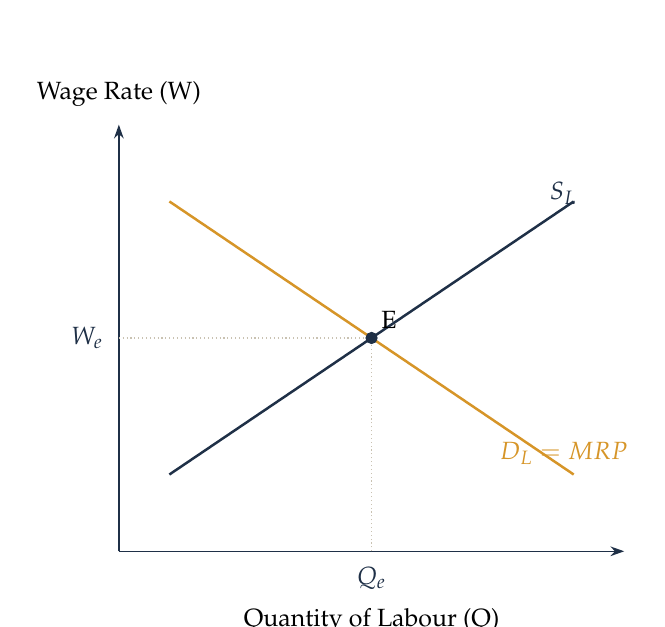
\begin{tikzpicture}[scale=1.0, baseline=(current bounding box.center)]
  \begin{axis}[econ chart,
    xlabel style={at={(ticklabel cs:0.5)}, anchor=north},
    width=8.0cm, height=7.0cm,
    xmin=0, xmax=100, ymin=0, ymax=100,
    xlabel={\small Quantity of Labour (Q)},
    ylabel={\small Wage Rate (W)},
    xtick={50}, xticklabels={$Q_e$},
    ytick={50}, yticklabels={$W_e$}
  ]
    \addplot[curve primary, domain=10:90] {0.8*x+10};
    \node[font=\small, color=CurveNavy] at (axis cs:88,84) {$S_L$};
    \addplot[curve accent, domain=10:90] {-0.8*x+90};
    \node[font=\small, color=CurveGold] at (axis cs:88,23) {$D_L = MRP$};
    \addplot[guide projection] coordinates {(50,0)(50,50)};
    \addplot[guide projection] coordinates {(0,50)(50,50)};
    \addplot[only marks, mark=*, mark size=2pt, color=CurveNavy] coordinates {(50,50)};
    \node[font=\small, above right] at (axis cs:50,50) {E};
  \end{axis}
\end{tikzpicture}%
}{%
\textbf{\color{NavyPrimary}Reading the diagram:}\\[4pt]
Supply of labour ($S_L$) slopes upward: workers will supply more hours at higher wages. Demand for labour ($D_L$) is the firm's MRP curve, sloping downward. Equilibrium occurs at point E, where $S_L$ and $D_L$ intersect. At this wage ($W_e$), the quantity of labour supplied equals the quantity demanded ($Q_e$). This is the market-clearing wage with zero unemployment. The vertical distance above this point represents a wage surplus (workers willing to work but no jobs), while below it represents a labour shortage (employers want to hire but insufficient workers available).%
}
\end{diagrambox}

\subsection{Wage Determination in Imperfect Markets}

Here, real-world ``imperfections'' disrupt the perfect market model.

\subsubsection{Trade Unions}

Unions act as a monopoly supplier of labour. They use collective bargaining to push wages above the market equilibrium (e.g., to $W_{Union}$). Effect: At this higher wage, the quantity of labour demanded falls (to $Q_D$) and the quantity supplied rises (to $Q_S$), creating unemployment ($Q_S - Q_D$).

\textbf{Elasticity of Demand for Labour is Crucial:} If demand for labour is inelastic (e.g., for highly skilled nuclear engineers), unions can push wages up significantly with little job loss. If it is elastic (e.g., for easily replaceable retail staff), wage rises lead to large job losses.

\subsubsection{Government -- National Minimum Wage (NMW)}

Sets a legal floor on wages ($W_{Min}$). Effect: Similar analysis to unions. If NMW is set above equilibrium (for low-skilled markets), it causes unemployment (excess supply of labour).

\begin{itemize}
  \item \textbf{Key Debate:} Supporters argue it increases incomes, reduces poverty, and may increase productivity. Critics highlight potential job losses, especially if the NMW is set very high or demand for labour is elastic.
\end{itemize}

\subsubsection{Monopsony Employers}

\begin{keyterm}{Monopsony}
A single buyer of labour in a market (e.g., a large factory in a small town, the NHS for nurses). To hire more workers, the monopsonist must raise the wage for all workers, making the Marginal Cost of Labour (MCL) $>$ Wage. The monopsonist maximises profit where MCL = MRP. It hires fewer workers ($Q_M$) and pays a lower wage ($W_M$) than in a competitive market ($Q$, $W$). This creates \textbf{monopsony exploitation} (the gap between MRP and the wage paid).
\end{keyterm}


\begin{diagrambox}[Trade Union / Minimum Wage Effect and Monopsony Labour Market]
\tworowwithtext{%
% --- Union / NMW above equilibrium ---------------------------------
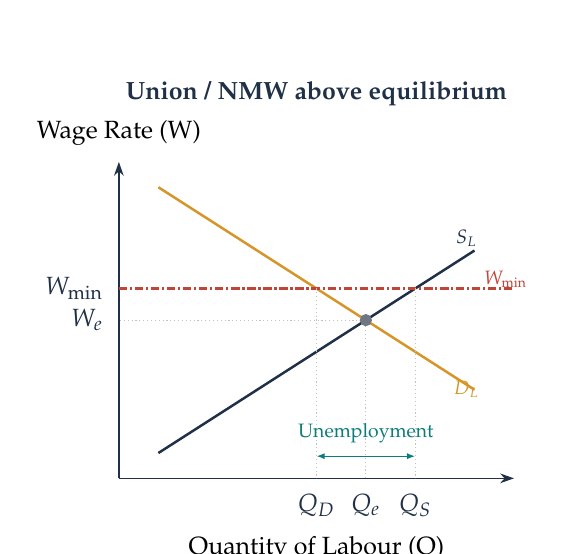
\begin{tikzpicture}[baseline=(current bounding box.center)]
  \begin{axis}[econ chart,
    width=6.6cm, height=5.6cm,
    xmin=0, xmax=100, ymin=0, ymax=100,
    xlabel={\small Quantity of Labour (Q)},
    ylabel={\small Wage Rate (W)},
    xlabel style={at={(ticklabel cs:0.5)}, anchor=north},
    xtick={50,62.5,75}, xticklabels={$Q_D$,$Q_e$,$Q_S$},
    ytick={50,60}, yticklabels={$W_e$,$W_{\min}$},
    title={\small\bfseries\color{CurveNavy} Union / NMW above equilibrium},
    title style={at={(0.5,1.06)}, anchor=south, yshift=4pt}
  ]
    \addplot[curve primary, domain=10:90] {0.8*x + 0};
    \node[font=\scriptsize\itshape, color=CurveNavy] at (axis cs:88,76) {$S_L$};
    \addplot[curve accent, domain=10:90] {-0.8*x + 100};
    \node[font=\scriptsize\itshape, color=CurveGold] at (axis cs:88,28) {$D_L$};
    \addplot[guide projection] coordinates {(62.5,0)(62.5,50)(0,50)};
    \addplot[only marks, mark=*, mark size=2pt, AnnotGray] coordinates {(62.5,50)};
    \addplot[price floor, domain=0:100] {60};
    \node[font=\scriptsize, color=CurveDanger, anchor=west] at (axis cs:90,63) {$W_{\min}$};
    \addplot[guide projection] coordinates {(50,60)(50,0)};
    \addplot[guide projection] coordinates {(75,60)(75,0)};
    \draw[{Latex[length=3pt]}-{Latex[length=3pt]}, color=CurveSage, line width=0.5pt]
      (axis cs:50,7) -- (axis cs:75,7);
    \node[font=\scriptsize, color=CurveSage, anchor=south] at (axis cs:62.5,8) {Unemployment};
  \end{axis}
\end{tikzpicture}
}{%
% --- Monopsony labour market ---------------------------------------
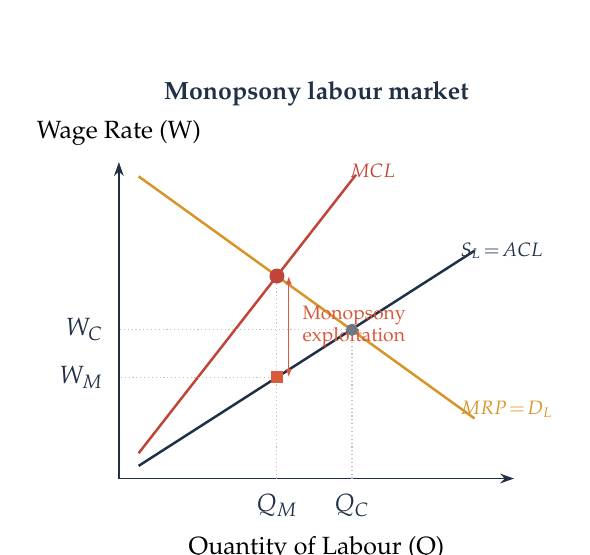
\begin{tikzpicture}[baseline=(current bounding box.center)]
  \begin{axis}[econ chart,
    width=6.6cm, height=5.6cm,
    xmin=0, xmax=100, ymin=0, ymax=100,
    xlabel={\small Quantity of Labour (Q)},
    ylabel={\small Wage Rate (W)},
    xlabel style={at={(ticklabel cs:0.5)}, anchor=north},
    xtick={40,59}, xticklabels={$Q_M$,$Q_C$},
    ytick={32,47}, yticklabels={$W_M$,$W_C$},
    title={\small\bfseries\color{CurveNavy} Monopsony labour market},
    title style={at={(0.5,1.06)}, anchor=south, yshift=4pt}
  ]
    \addplot[curve primary, domain=5:90] {0.8*x + 0};
    \node[font=\scriptsize\itshape, color=CurveNavy, anchor=west] at (axis cs:84,72) {$S_L\!=\!ACL$};
    \addplot[curve danger, domain=5:60] {1.6*x + 0};
    \node[font=\scriptsize\itshape, color=CurveDanger, anchor=south west] at (axis cs:56,92) {$MCL$};
    \addplot[curve accent, domain=5:90] {-0.9*x + 100};
    \node[font=\scriptsize\itshape, color=CurveGold, anchor=west] at (axis cs:84,22) {$MRP\!=\!D_L$};
    \addplot[guide projection] coordinates {(40,0)(40,64)};
    \addplot[guide projection] coordinates {(40,32)(0,32)};
    \addplot[guide projection] coordinates {(59,0)(59,47)(0,47)};
    \addplot[only marks, mark=*, mark size=2pt, AnnotGray] coordinates {(59,47)};
    \addplot[only marks, mark=*, mark size=2.5pt, color=CurveDanger] coordinates {(40,64)};
    \addplot[only marks, mark=square*, mark size=2pt, color=CurveRose] coordinates {(40,32)};
    % "Monopsony exploitation" arrow between W_M and MRP at Q_M
    \draw[{Latex[length=3pt]}-{Latex[length=3pt]}, color=CurveRose, line width=0.5pt]
      (axis cs:43,32) -- (axis cs:43,64);
    \node[font=\scriptsize, color=CurveRose, anchor=west, align=left] at (axis cs:44,48)
      {Monopsony\\exploitation};
  \end{axis}
\end{tikzpicture}%
}{%
\textbf{\color{CurveNavy}Union / NMW:} a wage floor at $W_{\min}>W_e$ raises supply to $Q_S$ but cuts demand to $Q_D$, creating unemployment of $Q_S-Q_D$ (green arrow).\quad
\textbf{\color{CurveNavy}Monopsony:} a single buyer faces upward-sloping $ACL$, so $MCL$ lies above it.  Profit-max at $MCL=MRP$ gives $Q_M<Q_C$, with the wage read from $ACL$ at $W_M<W_C$ -- the gap $W_M\!\to\!MRP$ is the firm's \textit{exploitation}.  Counter-intuitively, a well-set minimum wage in a monopsony can raise \textit{both} wages and employment.%
}
\end{diagrambox}

\subsection{Wage Differentials}

\begin{keyterm}{Wage Differentials}
Differences in pay between different jobs, industries, or workers. Causes (always explain via D\&S):
\begin{itemize}
  \item \textbf{Differences in Demand:} High demand for rare skills (brain surgeons, AI specialists) $\rightarrow$ high wages.
  \item \textbf{Differences in Supply:} Jobs requiring long training (supply is limited) or with unpleasant conditions (danger, unsocial hours) need a \textbf{compensating differential} (higher wage) to attract workers.
\end{itemize}
\end{keyterm}

\subsection{Transfer Earnings \& Economic Rent}

\begin{keyterm}{Transfer Earnings}
The minimum payment required to keep a factor of production (e.g., a worker) in its current use. It's the wage they could earn in their next best alternative occupation.
\end{keyterm}

\begin{keyterm}{Economic Rent}
Any payment above the transfer earnings. It's a ``surplus'' the worker enjoys.
\end{keyterm}

\begin{example}[Transfer Earnings and Economic Rent]
A brain surgeon earning £200,000 whose next best job pays £40,000 has Transfer Earnings = £40k and Economic Rent = £160k.
\end{example}

\textbf{Explanation \& Link to Elasticity:}
\begin{itemize}
  \item The more \textbf{inelastic} the supply of labour (unique skills, natural talent), the greater the proportion of their income that is economic rent. (Think: Premier League footballer).
  \item The more \textbf{elastic} the supply of labour (unskilled work with many alternatives), the lower the economic rent. Their wage is very close to their transfer earnings.
\end{itemize}



\begin{diagrambox}[Transfer Earnings and Economic Rent -- Area Diagram]
\diagramwithtext{%
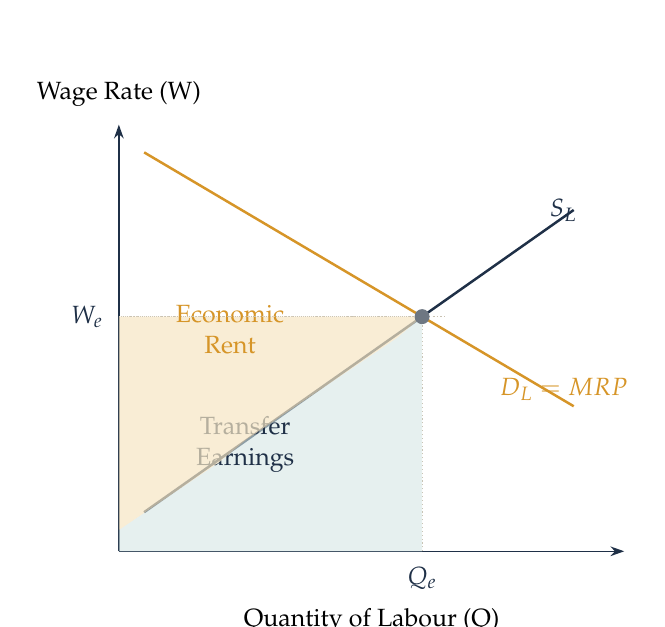
\begin{tikzpicture}[scale=1.0, baseline=(current bounding box.center)]
  \begin{axis}[econ chart,
    xlabel style={at={(ticklabel cs:0.5)}, anchor=north},
    width=8.0cm, height=7.0cm,
    xmin=0, xmax=100, ymin=0, ymax=100,
    xlabel={\small Quantity of Labour (Q)},
    ylabel={\small Wage Rate (W)},
    xtick={60}, xticklabels={$Q_e$},
    ytick={55}, yticklabels={$W_e$}
  ]
    % Supply curve (upward sloping)
    \addplot[curve primary, domain=5:90] {(5/6)*x + 5};
    \node[font=\small, color=CurveNavy] at (axis cs:88,80) {$S_L$};
    % Demand (MRP)
    \addplot[curve accent, domain=5:90] {-0.7*x + 97};
    \node[font=\small, color=CurveGold] at (axis cs:88,38) {$D_L = MRP$};
    % Equilibrium
    \addplot[guide projection] coordinates {(60,0)(60,55)(0,55)};
    \addplot[only marks, mark=*, mark size=2.5pt, AnnotGray] coordinates {(60,55)};
    % Transfer earnings = area under supply curve up to Q_e
    \addplot[fill=FillPrimary, opacity=0.6, draw=none]
      coordinates {(0,5)(5,9)(10,13)(15,17)(20,21)(25,26)(30,30)(35,34)(40,38)(45,42)(50,46)(55,50)(60,55)(60,0)(0,0)};
    \node[font=\small, color=CurveNavy, align=center] at (axis cs:25,25) {Transfer\\Earnings};
    % Economic rent = area between wage line and supply curve
    \addplot[fill=FillGold, opacity=0.7, draw=none]
      coordinates {(0,55)(5,55)(10,55)(15,55)(20,55)(25,55)(30,55)(35,55)(40,55)(45,55)(50,55)(55,55)(60,55)(55,50)(50,46)(45,42)(40,38)(35,34)(30,30)(25,26)(20,21)(15,17)(10,13)(5,9)(0,5)};
    \node[font=\small, color=CurveGold, align=center] at (axis cs:22,52) {Economic\\Rent};
    % Wage line
    \addplot[guide projection, domain=0:65] {55};
  \end{axis}
\end{tikzpicture}%
}{%
\textbf{\color{NavyPrimary}Reading the diagram:}\\[4pt]
Transfer earnings (shaded blue) is the minimum payment needed to keep a worker in their current job---the area under the supply curve. It equals what they could earn in their next best occupation. Economic rent (shaded gold) is any payment above transfer earnings: the surplus they enjoy. With highly inelastic supply (e.g., top surgeons, athletes), economic rent is large because few people can do the job. With elastic supply (e.g., unskilled retail), economic rent is small because the wage is close to transfer earnings.%
}
\end{diagrambox}


\begin{tcolorbox}[enhanced,colback=EvalBg,colframe=EvalFrame,arc=0pt,boxrule=1pt,title={\bfseries\color{EvalFrame}Evaluation: Labour Markets, Wages and Equity},fonttitle=\small]
\small\RaggedRight
\begin{itemize}[itemsep=2pt,topsep=2pt]
  \item \textbf{NMW -- monopsony exception:} Standard competitive theory predicts a minimum wage above equilibrium causes unemployment. But in a \textit{monopsony}, a minimum wage can \textit{raise both wages and employment} simultaneously. \textit{``The effect depends on the degree of employer market power.''}
  \item \textbf{NMW -- elasticity matters:} If labour demand is inelastic (e.g.\ skilled workers with no substitutes), a NMW creates little unemployment. If demand is elastic (low-skilled, easily automated), job losses can be significant.
  \item \textbf{Equity vs.\ efficiency:} Progressive taxation and generous benefits reduce inequality but may reduce the incentive to work (poverty trap) and to invest (if corporation tax is high). There is a genuine trade-off.
  \item \textbf{Transfer payments -- disincentive effect:} Means-tested benefits that phase out as income rises create very high marginal effective tax rates (up to 80\%+). This can trap recipients in low-paid work. Universal Basic Income avoids this but is extremely costly.
  \item \textbf{Economic rent -- policy implication:} Workers with highly inelastic labour supply (top athletes, surgeons) receive large economic rents. A tax on this rent does \textit{not} reduce supply or efficiency, making it an efficient redistributive instrument.
  \item \textbf{Trade unions -- declining power:} Globalisation and automation have reduced union bargaining power in many countries. The wage premium from union membership has fallen significantly since the 1980s.
\end{itemize}
\end{tcolorbox}

\begin{evaluation}{Minimum Wage: Who Benefits, Who Loses?}
\textbf{Strengths / Arguments For National Minimum Wage:}
\begin{itemize}[leftmargin=*, nosep]
\item Increases incomes for low-paid workers; reduces poverty and relative income inequality.
\item May increase productivity if better-paid workers are more motivated and healthier.
\item Reduces exploitation in monopsony labour markets; particularly effective in concentrated industries (meat processing, care work).
\item Reduces in-work poverty without expanding means-tested welfare (no poverty trap stigma).
\end{itemize}
\textbf{Limitations / Arguments Against Minimum Wage:}
\begin{itemize}[leftmargin=*, nosep]
\item Causes unemployment and reduced hours for low-skilled workers if demand for labour is elastic.
\item Hurts young, unskilled, and disabled workers most (they are priced out of entry-level jobs).
\item May force firms to cut non-wage benefits (training, flexibility) to offset wage costs.
\item Doesn't target the poor specifically; high earners benefit if they work part-time at minimum wage.
\item May accelerate automation (firms replace workers with machines).
\end{itemize}
\textbf{Monopsony Exception (Nuance):}
\begin{itemize}[leftmargin=*, nosep]
\item In a monopsony (single large employer), a minimum wage can raise both wages and employment.
\item Firm is forced to move along upward-sloping labour supply curve; if wage floor is below monopoly exploitation point, employment increases.
\item Evidence from fast-food industry and care homes suggests some NMW effects are positive on employment.
\end{itemize}
\textbf{It depends on\ldots}
\begin{itemize}[leftmargin=*, nosep]
\item Labour market structure: monopsony exception is real, but most low-wage markets are competitive.
\item Elasticity of labour demand: young, unskilled workers face elastic demand; skilled workers face inelastic demand.
\item Level of minimum wage: small increases above equilibrium have modest employment effects; large increases cause significant job loss.
\item Geographic variation: rural low-wage areas may suffer more than high-wage urban areas.
\item Complementary policies: training and education programs can cushion job loss effects.
\end{itemize}
\end{evaluation}

\begin{evaluation}{Trade Unions: Wage Effects, Employment Effects, and Equity}
\textbf{Strengths / Arguments For Trade Unions:}
\begin{itemize}[leftmargin=*, nosep]
\item Collective bargaining power raises wages above competitive level (wage premium: 10-20\% in many economies).
\item Improves working conditions, health and safety standards (often ahead of regulation).
\item Reduces inequality between unionised and non-unionised workers; compresses wage distribution.
\item Provides voice and procedural justice; workers have say in disputes (grievance procedures).
\item Historical role: unions fought for weekends, child labour bans, 8-hour day (now taken for granted).
\end{itemize}
\textbf{Limitations / Arguments Against Trade Unions:}
\begin{itemize}[leftmargin=*, nosep]
\item Restrict labour supply (high union fees, closed shops, apprenticeship limits) and raise wages for members at cost of non-union workers.
\item Create unemployment if wage demands exceed workers' marginal revenue product; insiders gain, outsiders (youth, unskilled) lose.
\item Lead to strikes and industrial disruption; deadweight loss to economy and consumers.
\item May entrench inefficient work practices (restrictive practises) and slow innovation and restructuring.
\item May reduce international competitiveness if union wages push costs above world prices; leads to import competition and job loss.
\end{itemize}
\textbf{Bilateral Monopoly Framework:}
\begin{itemize}[leftmargin=*, nosep]
\item Monopsony employer facing unionised monopoly supplier of labour: outcome indeterminate (between monopsony wage and competitive wage).
\item Bargaining power and credibility of threats determine outcome; wage could be anywhere between $W_M$ and $W_C$.
\item Strikes and lockouts are costly to both sides; often settle between extremes.
\end{itemize}
\textbf{It depends on\ldots}
\begin{itemize}[leftmargin=*, nosep]
\item Industry structure: monopsony vs. competitive labour market (effect is very different).
\item Union strength: centralised, powerful unions have more wage-setting power; weak, fragmented unions have less.
\item Economic conditions: in booms, unions capture productivity gains; in recessions, wage rigidity causes unemployment.
\item Labour market regulations: strong employment protections and high minimum wages reduce union power (less premium to gain).
\item Global competition: exposed sectors (manufacturing) face import competition; unions must moderate or jobs move.
\end{itemize}
\end{evaluation}

\begin{evaluation}{Government Intervention in Labour Markets (Trade-offs)}
\textbf{Strengths / Arguments For Government Intervention:}
\begin{itemize}[leftmargin=*, nosep]
\item Market failure (monopsony, information asymmetry, discrimination) justifies correction.
\item Protects vulnerable groups (young workers, disabled, migrants) from exploitation.
\item Provides social insurance (unemployment benefits, maternity leave) that individual cannot self-insure.
\item Corrects equity: progressive wages and benefits reduce inequality and relative poverty.
\end{itemize}
\textbf{Limitations / Arguments Against Intervention:}
\begin{itemize}[leftmargin=*, nosep]
\item Creates labour market rigidities; high hiring/firing costs reduce job creation and labour mobility.
\item Increases unemployment (especially youth unemployment) if regulations price workers out of market.
\item Reduces work incentives: high taxes and generous benefits create poverty trap and reduce labour supply.
\item Increases compliance costs for firms, especially small businesses; may reduce investment and growth.
\item Government failure risk: policies may be poorly designed, captured by special interests, or create unintended consequences.
\end{itemize}
\textbf{Types of Intervention (and Trade-offs):}
\begin{itemize}[leftmargin=*, nosep]
\item \textbf{Minimum wage:} Protects low-paid workers but may cost jobs; effectiveness depends on monopsony power and elasticity.
\item \textbf{Employment protection laws:} Secure jobs but discourage hiring; reduce labour market flexibility.
\item \textbf{Unemployment benefits:} Provide social insurance but reduce incentive to find work (moral hazard).
\item \textbf{Active labour market policies:} Training and job matching improve outcomes; cost-effective if well-designed.
\item \textbf{Anti-discrimination laws:} Ensure fair hiring but add compliance burden; effectiveness depends on enforcement.
\end{itemize}
\textbf{It depends on\ldots}
\begin{itemize}[leftmargin=*, nosep]
\item Labour market conditions: loose labour markets (high unemployment) justify more intervention; tight markets need less.
\item Type of market failure: monopsony justifies intervention; perfectly competitive market does not.
\item Design quality: well-designed policies (e.g., active labour policies) have high returns; poorly designed policies waste resources.
\item Complementarity: labour market policies work better with education, training, and macroeconomic stability.
\end{itemize}
\end{evaluation}

\begin{evaluation}{Equity vs. Efficiency Trade-off}
\textbf{Strengths / Arguments For Prioritising Equity:}
\begin{itemize}[leftmargin=*, nosep]
\item Market outcomes are often unfair: inherited wealth, luck, and privilege create inequality unrelated to effort or merit.
\item Poverty is a real hardship with external costs (crime, health, social breakdown); redistribution improves total welfare.
\item Diminishing marginal utility of income: £1 to poor person worth more than £1 to rich person; redistribution increases total utility.
\item Social cohesion and stability: extreme inequality breeds resentment, social unrest, and political instability.
\item Equal opportunity (not outcome) requires redistribution to level playing field; help poor children access education.
\end{itemize}
\textbf{Strengths / Arguments For Prioritising Efficiency:}
\begin{itemize}[leftmargin=*, nosep]
\item Redistribution reduces work incentives; high marginal tax rates discourage labour supply and investment (poverty trap).
\item Inequality reflects productivity differences; unequal pay rewards talent and effort, encouraging excellence and growth.
\item Large welfare state is costly to administer and finance; deadweight loss from taxation; opportunity cost.
\item Innovation and entrepreneurship driven by profit motive; too much redistribution kills incentive to take risks.
\item Efficient economy grows faster and creates more jobs; larger pie benefits everyone, even poor.
\end{itemize}
\textbf{The Empirical Trade-off:}
\begin{itemize}[leftmargin=*, nosep]
\item Evidence is mixed: some countries (Nordics) combine high equity with strong growth; others show equity-efficiency tension.
\item Marginal tax rates above 60-70\% show clear labour supply disincentives; rates below this are debated.
\item Inequality at very high levels (Gini > 0.50) is correlated with slower growth; some redistribution improves efficiency (reduces wasted talent, improves health).
\end{itemize}
\textbf{It depends on\ldots}
\begin{itemize}[leftmargin=*, nosep]
\item Current level of inequality: highly unequal society benefits more from redistribution; more equal societies lose from it.
\item Elasticity of labour supply: if workers are not responsive to taxes, redistribution has less efficiency cost.
\item Type of redistribution: transfers to productive activities (education, training) can increase growth; transfers for consumption reduce it.
\item Time horizon: short-run equity can hurt long-run efficiency; intergenerational effects matter.
\item Alternative policies: matching grants (e.g., education) may reduce inequality with less efficiency loss than cash transfers.
\end{itemize}
\end{evaluation}

\begin{evaluation}{Progressive Taxation vs. Flat Tax}
\textbf{Strengths / Arguments For Progressive Taxation:}
\begin{itemize}[leftmargin=*, nosep]
\item Maximises social welfare if marginal utility of income diminishes; takes more from those who lose less utility.
\item Reduces inequality and funds welfare state and public services used by poor (healthcare, education).
\item Aligns with ability-to-pay principle (horizontal and vertical equity): those who earn more contribute more.
\item Reflects societal preference for redistribution and fairness (progressive taxes are politically popular in democracies).
\end{itemize}
\textbf{Strengths / Arguments For Flat Tax:}
\begin{itemize}[leftmargin=*, nosep]
\item Simple and transparent; easy to understand and calculate (no complex brackets).
\item Reduces tax avoidance and evasion (lower incentive to hide income or relocate); broadens tax base.
\item Improves work incentives; same marginal rate for all means high earners not penalised for earning more.
\item Spurs investment and entrepreneurship; money not taken by government can be invested in business.
\item May increase economic growth; higher growth can raise total tax revenue even at lower rate (Laffer curve).
\end{itemize}
\textbf{Empirical Evidence:}
\begin{itemize}[leftmargin=*, nosep]
\item Nordic countries with high progressive taxes have strong growth and innovation (e.g., Apple, IKEA models emerge from high-tax countries).
\item Central European flat tax countries (Slovakia, Romania) showed weak growth; not clear if tax structure or other factors responsible.
\item Labour supply elasticity: high earners show some response to tax rate changes; low earners show little.
\item Tax competition: if one country raises top rate sharply, high earners relocate (``brain drain''); limits progressivity in open economies.
\end{itemize}
\textbf{Practical Hybrids:}
\begin{itemize}[leftmargin=*, nosep]
\item Most real systems use progressive income tax combined with regressive consumption tax (VAT), flattening overall progressivity.
\item Wealth taxes (capital gains, inheritance tax) are often less progressive than income tax.
\item Corporate tax flat rate with higher top personal income tax is common compromise.
\end{itemize}
\textbf{It depends on\ldots}
\begin{itemize}[leftmargin=*, nosep]
\item Labour supply elasticity: more elastic supply favours flatter tax; less elastic allows more progression.
\item Mobility of capital and labour: open economy with high mobility limits progressivity; closed economy can afford more.
\item Income distribution: more unequal society may need more progression to fund redistribution.
\item Political philosophy: egalitarian societies prefer progressive; libertarian societies prefer flat or low tax.
\item Complementary policies: strong unemployment benefits reduce incentive for flat tax (already cushioning low earners).
\end{itemize}
\end{evaluation}

\subsection{Exam Practice Questions -- Chapter 8: Government Policy, Equity and the Labour Market}

\begin{exampractice}
\textbf{Question 1: Market Failure and Government Intervention}

A market for cigarettes has negative consumption externalities (second-hand smoke harms non-smokers). The competitive equilibrium is P = £5, Q = 50 million packs/year. The marginal external cost (MEC) is £2 per pack.

\begin{enumerate}[label=(\alph*)]
\item Draw a diagram showing the competitive equilibrium and the socially optimal output (where P = MB + MEB). Calculate the deadweight loss. [5 marks]
\item The government imposes a £2 excise tax per pack. Assuming demand is $P = 10 - 0.0001Q$, calculate the new price, quantity, and tax revenue. Explain how the tax corrects the externality. [5 marks]
\item Evaluate whether a tax is a better policy than regulation (a ban) or information campaigns. [4 marks]
\end{enumerate}
\end{exampractice}

\begin{exampractice}
\textbf{Question 2: Government Failure}

A government imposes a maximum rent control at £400/month in a housing market where the competitive equilibrium rent is £600 and equilibrium quantity is 10,000 units. Assume demand is P = 1000 - 0.04Q.

\begin{enumerate}[label=(\alph*)]
\item Calculate the quantity of housing demanded and supplied at the price ceiling. What is the shortage? [3 marks]
\item Explain the consequences of this price control: deadweight loss, quality reduction, black markets. [5 marks]
\item Evaluate whether the rent control is a case of government failure and discuss alternative policies (e.g.\ housing subsidies) that might better achieve affordable housing. [5 marks]
\end{enumerate}
\end{exampractice}

\begin{exampractice}
\textbf{Question 3: The Minimum Wage and Labour Market Effects}

In a market for casual workers, the demand for labour (MRP) is $W = 20 - 0.1L$ and the supply of labour is $W = 5 + 0.05L$ (where L is quantity of workers, W is wage in £/hour).

\begin{enumerate}[label=(\alph*)]
\item Calculate the competitive equilibrium wage and employment. [3 marks]
\item The government sets a minimum wage of £10/hour. Calculate employment and unemployment. Who benefits and who loses? [5 marks]
\item Discuss the monopsony exception: explain how a minimum wage could increase both wages and employment if the market were a monopsony. [4 marks]
\end{enumerate}
\end{exampractice}

\begin{exampractice}
\textbf{Question 4: Trade Unions and Labour Market Power}

A unionised firm faces supply of labour $W = 10 + 0.2L$ and MRP = $50 - 0.5L$. The union sets a wage of £18/hour.

\begin{enumerate}[label=(\alph*)]
\item How many workers will the firm hire at W = £18? Compare this to the competitive outcome (where $MRP = W$). Calculate the unemployment. [4 marks]
\item Show the monopsony exploitation gap if the firm were a monopsonist without a union. Compare the union outcome to monopsony. [4 marks]
\item Evaluate the trade-off: do unions benefit low-wage workers on balance, given that some outsiders are priced out? [4 marks]
\end{enumerate}
\end{exampractice}

\begin{exampractice}
\textbf{Question 5: Equity, Efficiency, and Redistribution Policy}

\begin{enumerate}[label=(\alph*)]
\item Define the equity-efficiency trade-off and explain why it exists using a poverty trap example. [4 marks]
\item A country introduces a means-tested benefit that is withdrawn at 80\% as income rises. A worker earning £10,000/year can receive £5,000 benefit. Calculate the marginal effective tax rate (METR) on earnings between £10,000 and £15,000 if the income tax rate is 20\%. [4 marks]
\item Evaluate three policy options to achieve equity while minimising efficiency loss: (i) means-tested benefits, (ii) Universal Basic Income, (iii) Negative Income Tax. Which is most promising and why? [5 marks]
\end{enumerate}
\end{exampractice}

% ============================================================
%  CHAPTER 9: THE MACROECONOMY - INCOME, GROWTH AND MONEY
% ============================================================
\chapter{The Macroeconomy: Income, Growth and Money}

% ─────────────────────────────────────────────────────────────
\section{The Circular Flow of Income}

\subsection{The Multiplier Process}

\subsubsection{The Circular Flow of Income: The Big Picture}

Imagine the economy as a circular flow of money between households and firms. Households supply factors of production (labour, land, capital) to firms and earn income (wages, rent, profit, interest). They spend this income on goods and services produced by firms (Consumption, C). This spending becomes revenue for firms, who use it to pay for the factors of production, and the cycle continues.

\begin{itemize}
  \item \textbf{Injections (J)} add spending into the flow: Investment (I), Government Spending (G), and Exports (X).
  \item \textbf{Withdrawals/Leakages (W)} remove spending from the flow: Savings (S), Taxes (T), and Imports (M).
\end{itemize}

Equilibrium National Income occurs when Total Injections = Total Withdrawals (J = W), or equivalently, when Aggregate Demand (AD) = Aggregate Supply (AS).

\subsubsection{The Meaning of the Multiplier}

\begin{keyterm}{The Multiplier}
The ratio of the final change in national income to the initial change in an injection of AD (like I, G, or X). It explains how a small initial increase in spending can lead to a much larger final increase in national income.
\end{keyterm}

\textbf{Why does it happen?} An initial increase in spending (e.g., a new £1bn factory) becomes income for construction workers, suppliers, etc. They save some, pay tax on some, and spend on imports, but what's left they spend domestically (Consumption). This second round of spending becomes income for others, who again spend a part of it. This process repeats, with each round getting smaller, causing a multiplied total increase in national income.

\subsubsection{Key Formulae: Average (AP) and Marginal (MP) Propensities}

\begin{itemize}
  \item \textbf{Average Propensity (APx):} The proportion of total income used for a purpose. APC = Total Consumption / Total Income.
  \item \textbf{Marginal Propensity (MPx):} The proportion of an additional £1 of income used for a purpose. This is crucial for the multiplier.
\end{itemize}

You MUST know these:
\begin{itemize}
  \item \textbf{Marginal Propensity to Consume (MPC):} $\Delta C / \Delta Y$ (Change in Consumption / Change in Income)
  \item \textbf{Marginal Propensity to Save (MPS):} $\Delta S / \Delta Y$
  \item \textbf{Marginal Propensity to Import (MPM):} $\Delta M / \Delta Y$
  \item \textbf{Marginal Rate of Tax (MRT):} $\Delta T / \Delta Y$ (Often just called the marginal propensity to tax, MPT)
\end{itemize}

\begin{coreidea}
A fundamental relationship: $MPC + MPS + MPT + MPM = 1$. Every extra £1 of income is either consumed, saved, taxed, or spent on imports.
\end{coreidea}

\subsubsection{Multiplier Formulae \& Calculations}

\textbf{1. Closed Economy, No Government (Just Firms \& Households):}

Withdrawals = Savings only.
\[ k = \frac{1}{MPS} \quad \text{or} \quad \frac{1}{1 - MPC} \quad \text{(Since MPC + MPS = 1)} \]

\begin{example}[]
If MPC = 0.8, MPS = 0.2. $k = 1/0.2 = 5$. An initial £100m investment increases national income by £500m.
\end{example}

\textbf{2. Closed Economy, With Government:}

Withdrawals = Savings + Taxes.
\[ k = \frac{1}{MPS + MPT} \quad \text{or} \quad \frac{1}{1 - MPC} \]
(It's the same formula, but MPC is now the proportion of disposable income consumed.)
\begin{example}[]
If MPS = 0.15, MPT = 0.25. $k = 1/(0.15 + 0.25) = 1/0.4 = 2.5$.
\end{example}

\textbf{3. Open Economy, With Government (Most Realistic):}

Withdrawals = Savings + Taxes + Imports.
\[ k = \frac{1}{MPS + MPT + MPM} \]
\begin{example}[]
If MPS = 0.1, MPT = 0.2, MPM = 0.3. $k = 1/(0.1+0.2+0.3) = 1/0.6 \approx 1.67$.
\end{example}

Calculating the Effect on National Income:
\[ \Delta \text{National Income} = \Delta \text{Injection (I, G, or X)} \times \text{Multiplier } (k) \]

\subsubsection{National Income Determination: The 45° Diagram (Keynesian Cross)}

This diagram shows how equilibrium national income is determined.
\begin{itemize}
  \item \textbf{X-axis:} Real National Income (Y)
  \item \textbf{Y-axis:} Aggregate Demand (AD = C + I + G + (X-M))
  \item \textbf{The 45° line:} Represents all points where AD = Y (the equilibrium condition). It's a guideline.
  \item \textbf{The AD line:} Plots total planned expenditure at each income level. It has a positive slope (less than 45°) because as income rises, consumption rises (induced consumption).
  \item \textbf{Equilibrium:} Where the AD line cuts the 45° line. At this point, planned spending equals actual output/income.
\end{itemize}

\begin{diagrambox}[The Keynesian Cross (45° Diagram)]
\diagramwithtext{%
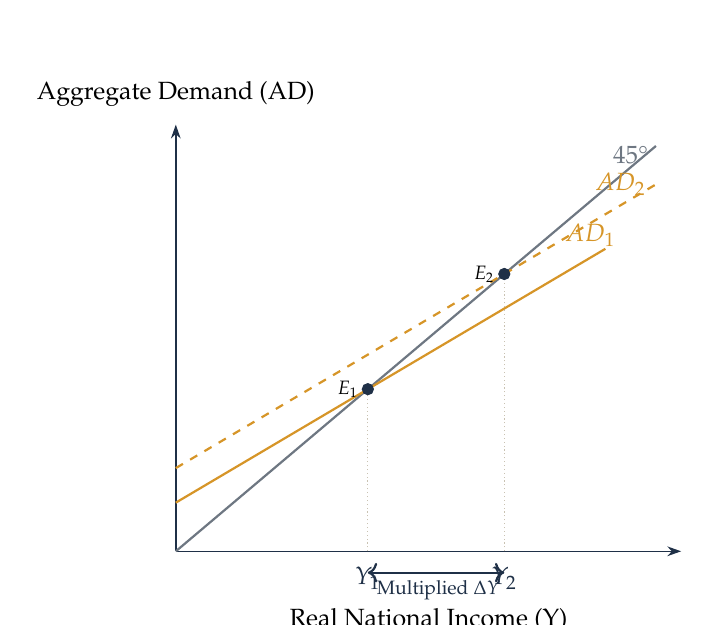
\begin{tikzpicture}[scale=1.0, baseline=(current bounding box.center)]
  \begin{axis}[econ chart,
    xlabel style={at={(ticklabel cs:0.5)}, anchor=north},
    width=8.0cm, height=7.0cm,
    xmin=0, xmax=100, ymin=0, ymax=100,
    xlabel={\small Real National Income (Y)},
    ylabel={\small Aggregate Demand (AD)},
    xtick={38,65}, xticklabels={$Y_1$,$Y_2$},
    ytick=\empty
  ]
    \addplot[thick, AnnotGray, domain=0:95] {x};
    \node[font=\small, AnnotGray] at (axis cs:90,93) {45°};
    \addplot[thick, CurveGold, domain=0:85] {0.7*x+11.4};
    \node[font=\small, CurveGold] at (axis cs:82,74) {$AD_1$};
    \addplot[thick, CurveGold, dashed, domain=0:95] {0.7*x+19.5};
    \node[font=\small, CurveGold] at (axis cs:88,86) {$AD_2$};
    \addplot[guide projection] coordinates {(38,0)(38,38)};
    \addplot[guide projection] coordinates {(65,0)(65,65)};
    \addplot[only marks, mark=*, mark size=2pt, CurveNavy] coordinates {(38,38)(65,65)};
    \node[font=\scriptsize, left] at (axis cs:38,38) {$E_1$};
    \node[font=\scriptsize, left] at (axis cs:65,65) {$E_2$};
    \draw[<->, thick, CurveNavy] (axis cs:38,-5) -- (axis cs:65,-5);
    \node[font=\scriptsize, CurveNavy] at (axis cs:52,-9) {Multiplied $\Delta Y$};
  \end{axis}
\end{tikzpicture}%
}{%
\textbf{\color{NavyPrimary}Reading the diagram:}\\[4pt]
The 45° line shows all points where aggregate demand (AD) equals output (Y)---the equilibrium condition. The AD line slopes upward (less steeply than 45°) because as income rises, consumption rises with it (induced consumption via the MPC). Equilibrium occurs at E$_1$, where AD$_1$ intersects the 45° line. When aggregate demand increases (AD$_1$ to AD$_2$), the new equilibrium E$_2$ is reached at a higher income level. The horizontal distance from Y$_1$ to Y$_2$ represents the multiplier effect: the increase in national income is larger than the vertical shift in AD, demonstrating how a change in autonomous expenditure is magnified through the multiplier.%
}
\end{diagrambox}

\textbf{Using the Multiplier on the Diagram:} An upward shift in the AD line (due to $\uparrow I$, $\uparrow G$, etc.) leads to a new, higher equilibrium income. The horizontal distance between the old and new equilibrium points is the change in national income, which is larger than the vertical shift in AD, demonstrating the multiplier effect.

\subsubsection{Reasons for Variations in the Size of the Multiplier}

The multiplier is larger when:
\begin{itemize}
  \item MPC is higher / MPS is lower (People spend more of extra income).
  \item MPT is lower (Lower tax rates leave more disposable income).
  \item MPM is lower (Lower propensity to import keeps spending within the domestic economy).
\end{itemize}
The multiplier is smaller when leakages (MPS, MPT, MPM) are larger.

\subsection{Components of Aggregate Demand (AD = C + I + G + (X-M))}

\subsubsection{Consumption (C): The Largest Component}

\begin{keyterm}{Consumption Function}
$C = a + bY_d$ where:
\begin{itemize}
  \item $a$ = Autonomous consumption (spending that happens even with zero income, via savings or borrowing).
  \item $b$ = MPC (the marginal propensity to consume).
  \item $Y_d$ = Disposable Income.
  \item $bY_d$ represents induced consumption (the part that depends on income).
\end{itemize}
\end{keyterm}

\subsubsection{Savings (S)}

$S = -a + sY_d$. The $-a$ = Dissaving to finance autonomous consumption when income is zero. $s$ = MPS. Savings is the complement of consumption ($S = Y_d - C$).

\subsubsection{Investment (I)}

\begin{itemize}
  \item \textbf{Autonomous Investment:} Determined by factors like interest rates, business confidence, technology, not directly by current national income.
  \item \textbf{Induced Investment \& The Accelerator:} Investment induced by changes in the level of national output. A rise in consumer demand ($\Delta C$) may require firms to invest in new capital goods to increase capacity.
\end{itemize}

\subsection{Accelerator Theory}

\begin{keyterm}{The Accelerator Principle}
The accelerator theory states that the level of net investment depends not on the \textit{level} of national income, but on the \textit{change} in national income. A rise in output causes firms to increase their capital stock to maintain the desired capital-to-output ratio.
$$I_{net} = v \times \Delta Y$$
Where $v$ is the \textbf{accelerator coefficient} (the capital-output ratio), and $\Delta Y$ is the change in national income.
\end{keyterm}

\subsubsection{The Capital-Output Ratio}

The accelerator coefficient $v$ represents how much capital a firm needs to produce each unit of output. If $v = 3$, a firm needs \pounds3 of capital to produce \pounds1 of output. This ratio is assumed constant in the simple model.

\subsubsection{Worked Numerical Example}

Suppose $v = 3$ and annual depreciation (replacement investment) is \pounds30m:

\begin{tcolorbox}[enhanced,colback=FillPrimary,colframe=GuideRule,arc=0pt,boxrule=0.8pt]
\begin{tabular}{@{}>{\RaggedRight\arraybackslash}p{0.06\linewidth}>{\RaggedRight\arraybackslash}p{0.14\linewidth}>{\RaggedRight\arraybackslash}p{0.14\linewidth}>{\RaggedRight\arraybackslash}p{0.20\linewidth}>{\RaggedRight\arraybackslash}p{0.20\linewidth}>{\RaggedRight\arraybackslash}p{0.14\linewidth}@{}}
\textbf{\color{CurveNavy}Year} & \textbf{\color{CurveNavy}Output (£m)} & \textbf{\color{CurveNavy}$\Delta$Y (£m)} & \textbf{\color{CurveNavy}Net Investment (£m)} & \textbf{\color{CurveNavy}Replacement (£m)} & \textbf{\color{CurveNavy}Gross I (£m)} \\
\midrule
1 & 100 & -- & 0 & 30 & 30 \\
2 & 120 & +20 & 60 & 30 & 90 \\
3 & 150 & +30 & 90 & 30 & 120 \\
4 & 160 & +10 & 30 & 30 & 60 \\
5 & 160 & 0 & 0 & 30 & 30 \\
6 & 155 & --5 & 0* & 30 & 30 \\
\end{tabular}
\end{tcolorbox}

\textit{*Net investment cannot be negative in the short run -- firms cannot ``un-invest'' machinery immediately; it falls to zero.}

\begin{coreidea}
\textbf{Key insight:} Output only \emph{slowed} from Year 3 to Year 4, but gross investment \emph{halved}. This is the accelerator in action. Output is still \emph{rising}, but because the \emph{rate} of increase fell, investment collapsed.
\end{coreidea}

\subsubsection{The Multiplier--Accelerator Interaction}

The accelerator works alongside the multiplier to amplify business cycle fluctuations:

\begin{enumerate}
  \item A rise in consumer demand ($\Delta C$) increases national income via the multiplier.
  \item Higher income triggers new investment via the accelerator ($I_{net} = v \times \Delta Y$).
  \item That investment itself raises income further via the multiplier.
  \item This creates a self-reinforcing cycle of expansion -- and equally sharp contraction on the way down.
\end{enumerate}

\subsubsection{Limitations of the Accelerator Theory}

\begin{itemize}
  \item \textbf{Spare capacity:} If firms have unused capital, they do not need to invest when output rises. The accelerator does not operate.
  \item \textbf{Business confidence:} Firms may not invest even if output rises if they expect the upturn to be temporary. ``Animal spirits'' (Keynes) matter.
  \item \textbf{Interest rates:} The cost of borrowing affects investment independently of output changes.
  \item \textbf{Fixed capital-output ratio:} In reality, firms can substitute labour for capital, so $v$ is not constant.
  \item \textbf{Time lags:} There are lags between output changes, investment decisions, and actual capital installation.
\end{itemize}

\begin{example}[Common MCQ Trap]
``Output rises from \pounds200m to \pounds210m in Year 1, then from \pounds210m to \pounds215m in Year 2. What happens to induced investment?'' -- It \textbf{falls}, because $\Delta Y$ shrank from \pounds10m to \pounds5m, even though output is still \emph{rising}. Students who confuse the \emph{level} of output with the \emph{change} in output will incorrectly say investment rises.
\end{example}

\subsubsection{Government Spending (G)}

Treated as primarily autonomous (determined by policy, not current income).

\subsubsection{Net Exports (X-M)}

\begin{itemize}
  \item \textbf{Exports (X):} Autonomous (dependent on foreign income, exchange rates, not domestic income).
  \item \textbf{Imports (M):} $M = mY$ where $m$ = MPM. Imports are induced by domestic income.
\end{itemize}

\subsection{Full Employment vs.\ Equilibrium National Income}

\begin{keyterm}{Full Employment Level of National Income ($Y_{fe}$)}
The level of output produced when all available factors of production are employed (note: this includes the natural rate of unemployment, not zero unemployment).
\end{keyterm}

\begin{keyterm}{Equilibrium Level of National Income ($Y_{eq}$)}
The level where AD = AS. This can be at, below, or above the full employment level.
\end{keyterm}

\subsubsection{Inflationary and Deflationary Gaps}

These are measured at the full employment level of income ($Y_{fe}$).

\begin{keyterm}{Deflationary (Recessionary) Gap}
\textbf{Occurs when:} $Y_{eq} < Y_{fe}$. The equilibrium level of income is below full employment.

\textbf{Meaning:} There is a deficiency of AD. At $Y_{fe}$, total planned spending (AD) is less than full employment output (AS). This leads to unplanned inventory buildup, causing firms to lay off workers and reduce output. Unemployment rises. The economy has spare capacity.

\textbf{On the diagram:} At $Y_{fe}$, the AD line lies below the 45° line. The vertical distance between the AD line and the 45° line at $Y_{fe}$ is the size of the deflationary gap.
\end{keyterm}

\begin{keyterm}{Inflationary Gap}
\textbf{Occurs when:} $Y_{eq} > Y_{fe}$. The economy is trying to operate beyond its full employment capacity.

\textbf{Meaning:} At $Y_{fe}$, AD exceeds potential AS. This leads to excess demand, unplanned inventory depletion, and upward pressure on prices (demand-pull inflation). Output cannot sustainably increase because resources are already fully employed.

\textbf{On the diagram:} At $Y_{fe}$, the AD line lies above the 45° line. The vertical distance between the AD line and the 45° line at $Y_{fe}$ is the size of the inflationary gap.
\end{keyterm}

\begin{coreidea}
\textbf{Key Link to Policy:} Governments can use fiscal policy (changing G and T) to shift AD and close these gaps. Increase AD to close a deflationary gap, decrease AD to close an inflationary gap.
\end{coreidea}

% ─────────────────────────────────────────────────────────────
\section{Economic Growth and Sustainability}

\subsection{Actual Growth vs.\ Potential Growth}

\begin{keyterm}{Actual Economic Growth}
An increase in the real output of an economy (real GDP) over time. It's what we measure quarterly or annually -- the actual goods and services produced. It's shown by a movement inside or along the Production Possibility Curve (PPC).
\end{keyterm}

\begin{keyterm}{Potential Economic Growth}
An increase in the productive capacity of the economy over time. It represents what the economy could produce if all resources were fully and efficiently employed. It's shown by an outward shift of the PPC or the Long-Run Aggregate Supply (LRAS) curve.
\end{keyterm}

\begin{example}[The Factory Analogy]
Think of a factory. \textbf{Actual Growth:} Producing more this month by using existing machinery for longer hours (using spare capacity). \textbf{Potential Growth:} Installing new, better machinery or expanding the factory floor -- increasing its maximum possible output.
\end{example}

\subsection{Positive and Negative Output Gaps}

An Output Gap is the difference between actual GDP and potential GDP.

\begin{itemize}
  \item \textbf{Negative Output Gap:} Actual GDP $<$ Potential GDP. Conditions: The economy is producing below its capacity. There is spare capacity, high unemployment (especially cyclical), and low inflation pressure. This is typical during a recession or slowdown. On an AD/AS diagram, equilibrium is to the left of the LRAS curve.
  \item \textbf{Positive Output Gap:} Actual GDP $>$ Potential GDP. Conditions: The economy is producing temporarily above its sustainable capacity. Resources are used unsustainably intensively (e.g., workers doing excessive overtime, factories operating 24/7). This leads to labour shortages, upward pressure on wages, and demand-pull inflation. On an AD/AS diagram, equilibrium is to the right of the LRAS curve. It's often associated with a late-stage boom.
\end{itemize}


\begin{diagrambox}[Positive and Negative Output Gaps on the AD/AS Model]
\tworowwithtext{%
% --- Positive output gap (overheating) ----------------------------
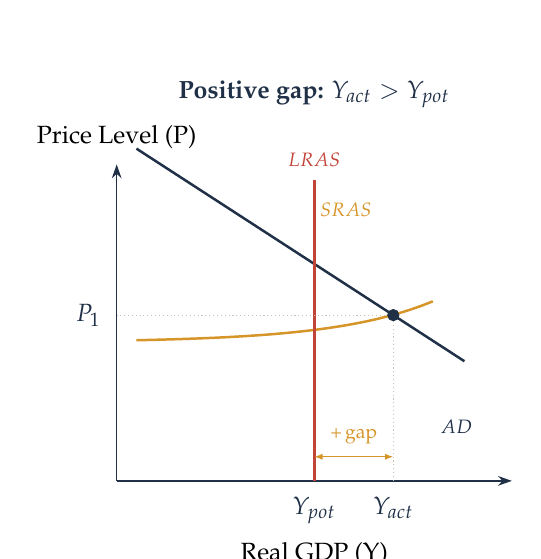
\begin{tikzpicture}[baseline=(current bounding box.center)]
  \begin{axis}[econ chart,
    width=6.6cm, height=5.6cm,
    xmin=0, xmax=100, ymin=0, ymax=105,
    xlabel={\small Real GDP (Y)},
    ylabel={\small Price Level (P)},
    xlabel style={at={(ticklabel cs:0.5)}, anchor=north},
    xtick={50,70}, xticklabels={$Y_{pot}$,$Y_{act}$},
    ytick={55}, yticklabels={$P_1$},
    title={\small\bfseries\color{CurveNavy} Positive gap: $Y_{act}>Y_{pot}$},
    title style={at={(0.5,1.06)}, anchor=south, yshift=4pt}
  ]
    \addplot[curve primary, domain=5:88] {-0.85*x + 114.5};
    \node[font=\scriptsize\itshape, color=CurveNavy] at (axis cs:86,18) {$AD$};
    \addplot[curve accent, domain=5:80, samples=60] {5*exp(0.04*(x-55))+46};
    \node[font=\scriptsize\itshape, color=CurveGold] at (axis cs:58,90) {$SRAS$};
    \addplot[curve danger] coordinates {(50,0)(50,100)};
    \node[font=\scriptsize\itshape, color=CurveDanger, anchor=south] at (axis cs:50,101) {$LRAS$};
    \addplot[guide projection] coordinates {(70,0)(70,55)(0,55)};
    \addplot[only marks, mark=*, mark size=2pt, AxisCharcoal] coordinates {(70,55)};
    \draw[{Latex[length=3pt]}-{Latex[length=3pt]}, color=CurveGold, line width=0.5pt]
      (axis cs:50,8) -- (axis cs:70,8);
    \node[font=\scriptsize, color=CurveGold, anchor=south] at (axis cs:60,9) {+\,gap};
  \end{axis}
\end{tikzpicture}
}{%
% --- Negative output gap (spare capacity) -------------------------
\begin{tikzpicture}[baseline=(current bounding box.center)]
  \begin{axis}[econ chart,
    width=6.6cm, height=5.6cm,
    xmin=0, xmax=100, ymin=0, ymax=105,
    xlabel={\small Real GDP (Y)},
    ylabel={\small Price Level (P)},
    xlabel style={at={(ticklabel cs:0.5)}, anchor=north},
    xtick={38,55}, xticklabels={$Y_{act}$,$Y_{pot}$},
    ytick={40}, yticklabels={$P_1$},
    title={\small\bfseries\color{CurveNavy} Negative gap: $Y_{act}<Y_{pot}$},
    title style={at={(0.5,1.06)}, anchor=south, yshift=4pt}
  ]
    \addplot[curve primary, domain=5:75] {-0.8*x + 70};
    \node[font=\scriptsize\itshape, color=CurveNavy] at (axis cs:72,12) {$AD$};
    \addplot[curve accent, domain=5:70, samples=60] {5*exp(0.04*(x-55))+37.5};
    \node[font=\scriptsize\itshape, color=CurveGold] at (axis cs:58,82) {$SRAS$};
    \addplot[curve danger] coordinates {(55,0)(55,100)};
    \node[font=\scriptsize\itshape, color=CurveDanger, anchor=south] at (axis cs:55,101) {$LRAS$};
    \addplot[guide projection] coordinates {(38,0)(38,40)(0,40)};
    \addplot[only marks, mark=*, mark size=2pt, AxisCharcoal] coordinates {(38,40)};
    \draw[{Latex[length=3pt]}-{Latex[length=3pt]}, color=CurveGold, line width=0.5pt]
      (axis cs:38,8) -- (axis cs:55,8);
    \node[font=\scriptsize, color=CurveGold, anchor=south] at (axis cs:46.5,9) {$-$\,gap};
  \end{axis}
\end{tikzpicture}%
}{%
\textbf{\color{CurveNavy}Positive output gap:} actual GDP exceeds potential.  The economy is operating above the $LRAS$ -- inflationary pressure builds and policy must \textit{cool} the economy.\quad
\textbf{\color{CurveNavy}Negative output gap:} actual GDP lies below potential.  Spare capacity, cyclical unemployment and deflationary pressure dominate -- the case for \textit{expansionary} policy.  $LRAS$ marks the sustainable, full-employment level of output; the goal of macro stabilisation is to close the gap.%
}
\end{diagrambox}

\subsection{Business (Trade) Cycle}

\begin{keyterm}{Business Cycle}
The fluctuations in real GDP around its long-term trend (potential growth). It consists of recurring periods of boom and slump.
\end{keyterm}

\textbf{Phases of the Cycle:}
\begin{itemize}
  \item \textbf{Boom/Peak:} High growth, low unemployment, high inflation, high confidence. Positive output gaps may appear.
  \item \textbf{Recession/Contraction/Downturn} (Two consecutive quarters of negative real GDP growth): Falling output, rising unemployment, falling inflation, low confidence.
  \item \textbf{Trough/Depression:} Output and confidence are at their lowest. High unemployment. Large negative output gap.
  \item \textbf{Recovery/Expansion/Upturn:} Output begins to rise, unemployment falls, confidence returns. The economy moves towards potential output.
\end{itemize}

\textbf{Causes of the Cycle:}
\begin{itemize}
  \item \textbf{Demand-side Shocks:} Sudden changes in aggregate demand (e.g., financial crisis 2008 $\rightarrow$ collapse in investment and consumption).
  \item \textbf{Supply-side Shocks:} Sudden changes in costs/productivity (e.g., oil price hikes 1970s, pandemic 2020 $\rightarrow$ reduced capacity).
  \item \textbf{Animal Spirits:} Waves of optimism/pessimism among investors and consumers.
  \item \textbf{Inventory Cycles:} Businesses building up and then depleting stocks.
\end{itemize}


\begin{diagrambox}[The Business (Trade) Cycle -- Phases of Fluctuation]
\diagramonly{%
\begin{tikzpicture}
  \begin{axis}[econ chart,
    width=14cm, height=6.2cm,
    xmin=0, xmax=100, ymin=30, ymax=100,
    xlabel={\small Time},
    ylabel={\small Real GDP},
    xlabel style={at={(ticklabel cs:0.5)}, anchor=north},
    xtick=\empty, ytick=\empty,
    clip=false
  ]
    % --- Long-run trend (dashed, neutral) ----------------------------
    \addplot[thick, color=AnnotGray, dashed, domain=0:100] {0.4*x + 45};
    \node[font=\scriptsize\itshape, color=AnnotGray, anchor=west]
        at (axis cs:96,85) {Trend};
    % --- The business cycle: sine wave around the trend --------------
    %    GDP(t) = trend + 15 sin(0.14 t)   (angle is in radians-equivalent)
    \addplot[curve primary, very thick, domain=0:100, samples=240]
        {0.4*x + 45 + 15*sin(deg(0.14*x))};
    % --- Phase labels --------------------------------------------------
    % Place each label well clear of the curve, anchored on the side
    % opposite the next phase, so they never overlap.
    \node[font=\scriptsize\bfseries, color=CurveSage, anchor=south]
        at (axis cs:11,82)   {Boom / Peak};
    \node[font=\scriptsize\itshape, color=CurveDanger, anchor=north]
        at (axis cs:25,55)   {Recession};
    \node[font=\scriptsize\bfseries, color=CurveDanger, anchor=north]
        at (axis cs:36,45)   {Trough};
    \node[font=\scriptsize\itshape, color=CurveSage, anchor=south]
        at (axis cs:47,68)   {Recovery};
    \node[font=\scriptsize\bfseries, color=CurveSage, anchor=south]
        at (axis cs:58,92)   {Boom / Peak};
    \node[font=\scriptsize\bfseries, color=CurveDanger, anchor=north]
        at (axis cs:80,55)   {Trough};
    % --- Output-gap brackets (above peak, below trough) ---------------
    \draw[{Latex[length=3pt]}-{Latex[length=3pt]}, color=CurveGold,
          line width=0.4pt]
        (axis cs:11,75) -- (axis cs:11,65.6);
    \node[font=\scriptsize, color=CurveGold, anchor=west]
        at (axis cs:12,70) {$+$\,gap};
    \draw[{Latex[length=3pt]}-{Latex[length=3pt]}, color=CurveGold,
          line width=0.4pt]
        (axis cs:36,52) -- (axis cs:36,58.4);
    \node[font=\scriptsize, color=CurveGold, anchor=west]
        at (axis cs:37,55) {$-$\,gap};
  \end{axis}
\end{tikzpicture}%
}%
\par\vspace{6pt}
{\small\color{AxisCharcoal}\RaggedRight
\textbf{\color{CurveNavy}Reading the diagram.}  Real GDP fluctuates around a long-run trend (dashed line).  The cycle has four recurring phases: \textit{boom/peak} -- high growth, low unemployment, building inflation; \textit{recession} -- falling output, rising unemployment; \textit{trough} -- lowest point, large negative output gap; \textit{recovery} -- output and confidence return.  The gold arrows mark output gaps: a positive gap near the peak (inflationary pressure) and a negative gap near the trough (spare capacity, unemployment).  These gaps are what stabilisation policy seeks to close.\par}
\end{diagrambox}

\subsubsection{Role of Automatic Stabilisers and Their Effects}

\begin{keyterm}{Automatic Stabilisers}
Mechanisms built into government finances that automatically reduce the size of economic fluctuations without deliberate policy changes.

\textbf{Key Examples:}
\begin{itemize}
  \item \textbf{Progressive Tax System:} In a boom, incomes rise, people move into higher tax brackets $\rightarrow$ government tax revenue rises automatically, dampening disposable income and AD. In a recession, tax revenue falls automatically, supporting disposable income.
  \item \textbf{Unemployment Benefits:} In a recession, unemployment rises $\rightarrow$ government spending on benefits rises automatically, supporting incomes and AD. In a boom, benefit spending falls.
\end{itemize}

\textbf{Effects:} They smooth the business cycle. They reduce the multiplier effect of shocks, making real GDP and employment more stable. They have a moderating effect on the price level by preventing excessive AD in booms and collapsing AD in recessions.
\end{keyterm}


\begin{diagrambox}[Inflationary and Deflationary Gaps -- Keynesian Cross]
\tworowwithtext{%
% --- Deflationary gap ---------------------------------------------
\begin{tikzpicture}[baseline=(current bounding box.center)]
  \begin{axis}[econ chart,
    width=6.6cm, height=5.6cm,
    xmin=0, xmax=100, ymin=0, ymax=100,
    xlabel={\small Real National Income (Y)},
    ylabel={\small Aggregate Demand (AD)},
    xlabel style={at={(ticklabel cs:0.5)}, anchor=north},
    xtick={50,65}, xticklabels={$Y_{eq}$,$Y_{fe}$},
    ytick=\empty,
    title={\small\bfseries\color{CurveNavy} Deflationary gap},
    title style={at={(0.5,1.06)}, anchor=south, yshift=4pt}
  ]
    \addplot[thick, color=AnnotGray, domain=0:95] {x};
    \node[font=\scriptsize, color=AnnotGray] at (axis cs:90,95) {$45^\circ$};
    \addplot[curve primary, domain=0:85] {0.7*x + 15};
    \node[font=\scriptsize\itshape, color=CurveNavy] at (axis cs:80,74) {$AD$};
    \addplot[guide projection] coordinates {(50,0)(50,50)};
    \addplot[guide projection] coordinates {(65,0)(65,65)};
    \addplot[only marks, mark=*, mark size=2pt, AxisCharcoal] coordinates {(50,50)};
    \addplot[guide projection] coordinates {(65,60.5)(0,60.5)};
    \draw[{Latex[length=3pt]}-{Latex[length=3pt]}, color=CurveDanger, line width=0.5pt]
      (axis cs:68,60.5) -- (axis cs:68,65);
    \node[font=\scriptsize, color=CurveDanger, anchor=west] at (axis cs:69,62.75) {Deflationary};
  \end{axis}
\end{tikzpicture}
}{%
% --- Inflationary gap ---------------------------------------------
\begin{tikzpicture}[baseline=(current bounding box.center)]
  \begin{axis}[econ chart,
    width=6.6cm, height=5.6cm,
    xmin=0, xmax=100, ymin=0, ymax=100,
    xlabel={\small Real National Income (Y)},
    ylabel={\small Aggregate Demand (AD)},
    xlabel style={at={(ticklabel cs:0.5)}, anchor=north},
    xtick={40,65}, xticklabels={$Y_{fe}$,$Y_{eq}$},
    ytick=\empty,
    title={\small\bfseries\color{CurveNavy} Inflationary gap},
    title style={at={(0.5,1.06)}, anchor=south, yshift=4pt}
  ]
    \addplot[thick, color=AnnotGray, domain=0:95] {x};
    \node[font=\scriptsize, color=AnnotGray] at (axis cs:90,95) {$45^\circ$};
    \addplot[curve primary, domain=0:85] {0.7*x + 19.5};
    \node[font=\scriptsize\itshape, color=CurveNavy] at (axis cs:80,82) {$AD$};
    \addplot[guide projection] coordinates {(65,0)(65,65)};
    \addplot[guide projection] coordinates {(40,0)(40,40)};
    \addplot[only marks, mark=*, mark size=2pt, AxisCharcoal] coordinates {(65,65)};
    \addplot[guide projection] coordinates {(40,47.5)(0,47.5)};
    \draw[{Latex[length=3pt]}-{Latex[length=3pt]}, color=CurveDanger, line width=0.5pt]
      (axis cs:42,40) -- (axis cs:42,47.5);
    \node[font=\scriptsize, color=CurveDanger, anchor=west] at (axis cs:43,43.75) {Inflationary};
  \end{axis}
\end{tikzpicture}
}{%
\textbf{\color{CurveNavy}Deflationary gap:} at the full-employment income $Y_{fe}$, planned $AD$ lies below the $45^\circ$ line, so equilibrium income $Y_{eq}<Y_{fe}$.  The vertical gap measures the shortfall in injections needed; expansionary fiscal/monetary policy is required to close it.\quad
\textbf{\color{CurveNavy}Inflationary gap:} at $Y_{fe}$, $AD$ lies \textit{above} the $45^\circ$ line, so equilibrium income exceeds full-employment.  The excess demand cannot be met by real output and spills into inflation; contractionary policy is required.  In both cases the gap is amplified by the multiplier.%
}
\end{diagrambox}

\subsection{Policies to Promote Economic Growth and Their Effectiveness}

\subsubsection{Increasing Quantity of Factor Inputs}

\begin{itemize}
  \item \textbf{Labour:} Policies to increase size/participation of workforce (e.g., raising retirement age, childcare subsidies, encouraging immigration).
  \item \textbf{Capital:} Policies to encourage investment in physical capital (e.g., lower interest rates, tax allowances on investment, stable political environment).
  \item \textbf{Land/Natural Resources:} Exploration and discovery (limited scope).
\end{itemize}
\textbf{Effectiveness:} Can increase potential output, but may face diminishing returns if not paired with improvements in quality/technology.

\subsubsection{Supply-Side Policies to Increase Productive Capacity (Quality/Efficiency)}

\begin{itemize}
  \item \textbf{Education \& Training:} Improves human capital $\rightarrow$ more productive workforce.
  \item \textbf{Investment in Infrastructure:} (e.g., transport, broadband) lowers business costs, increases efficiency.
  \item \textbf{Research \& Development (R\&D) Incentives:} Drives technological progress, the key to long-run growth.
  \item \textbf{Labour Market Reforms:} Making hiring/firing easier (flexibility) or reducing trade union power to reduce unemployment. (Note: Can impact equity).
  \item \textbf{Deregulation \& Privatisation:} Aimed at increasing competition and efficiency.
\end{itemize}
\textbf{Effectiveness:} Work to shift LRAS outwards. However, they are often slow-acting, expensive, and politically contentious. They can increase inequality.

\subsection{Inclusive Economic Growth}

\begin{keyterm}{Inclusive Economic Growth}
Economic growth that is broadly shared across society and creates opportunities for all. It's not just the size of the pie (GDP) increasing, but also about how the pie is divided. It combines growth with equity (fairness).
\end{keyterm}

\textbf{Impact on Equity and Equality:}
\begin{itemize}
  \item Growth can increase inequality: Gains often go initially to asset owners and skilled workers (Kuznets hypothesis). This worsens equality (the evenness of distribution).
  \item Inclusive growth aims to improve equity: It seeks to ensure the poorest benefit, improving social justice and social welfare.
\end{itemize}

\textbf{Policies to Promote Inclusive Growth:}
\begin{itemize}
  \item Progressive Taxation and Redistribution: Using tax and benefits to transfer income.
  \item Investing in Universal Public Services: Education, healthcare, and social protection for all.
  \item Minimum Wage Legislation: Raises incomes at the bottom.
  \item Anti-Discrimination Laws: Ensure equal opportunity in labour markets.
  \item Support for SMEs and Microfinance: Creates jobs and entrepreneurial opportunities for the less wealthy.
\end{itemize}

\subsection{Sustainable Economic Growth}

\begin{keyterm}{Sustainable Economic Growth}
Economic growth that meets the needs of the present without compromising the ability of future generations to meet their own needs. It balances economic, social, and environmental needs.
\end{keyterm}

\subsubsection{Using and Conserving Resources}

\begin{itemize}
  \item Shift from non-renewable (fossil fuels) to renewable resources (solar, wind).
  \item Improve resource efficiency (recycling, circular economy).
  \item Implement sustainable management of forests, fisheries, and water.
\end{itemize}

\subsubsection{Impact on Environment \& Climate Change}

\begin{itemize}
  \item \textbf{Negative:} Growth traditionally relies on energy/resource use $\rightarrow$ pollution, habitat loss, greenhouse gas emissions $\rightarrow$ climate change (global warming, extreme weather).
  \item \textbf{Potential Positive:} Higher GDP can lead to greater demand for a clean environment and more resources for green technology (Environmental Kuznets Curve hypothesis).
\end{itemize}

\subsubsection{Policies to Mitigate Impact / Reduce Carbon Emissions}

\textbf{Market-Based Policies:}
\begin{itemize}
  \item \textbf{Carbon Taxes:} A tax per tonne of CO$_2$ emitted. Increases cost of pollution, incentivises alternatives.
  \item \textbf{Cap-and-Trade (Emissions Trading Schemes):} Government sets a cap on total emissions and issues tradeable permits. Creates a market price for carbon.
\end{itemize}

\textbf{Government Regulation (Command \& Control):}
\begin{itemize}
  \item Legally Enforced Limits/Standards: e.g., fuel efficiency standards for cars, bans on single-use plastics.
\end{itemize}

\textbf{Government Provision \& Funding:}
\begin{itemize}
  \item Investment in Green Public Transport \& Renewable Energy.
  \item Subsidies for green technologies (e.g., electric vehicles, home insulation).
\end{itemize}

\textbf{Education \& Information:} Campaigns to encourage behavioural change (e.g., recycling, energy saving).

% ─────────────────────────────────────────────────────────────
\section{Employment/Unemployment}

\subsection{Definition of Full Employment}

\begin{keyterm}{Full Employment}
The meaning: Full employment does not mean zero unemployment. It means the lowest possible level of unemployment that a prosperous economy can sustain without creating excessive inflation. At this level, all available labour is being used efficiently. In other words, the only unemployment that exists is frictional and structural.
\end{keyterm}

\textbf{The problem of specifying a percentage:} Economists argue about the precise rate. In the 1960s, 2--3\% might have been considered full employment. Today, it's often thought to be around 4--5\% in many developed economies. The percentage changes because of:
\begin{itemize}
  \item Changes in the structure of the economy (e.g., shift from manufacturing to services).
  \item Demographic changes (e.g., more students, part-time workers).
  \item Changes in welfare benefits and job search technology.
  \item Hysteresis (see below): A prolonged recession can permanently raise the ``full employment'' rate.
\end{itemize}

\subsection{Equilibrium and Disequilibrium Unemployment}

\begin{keyterm}{Equilibrium Unemployment}
This occurs even when the labour market is in equilibrium (aggregate demand for labour = aggregate supply of labour). It consists of frictional (people between jobs) and structural (skills/regional mismatches) unemployment. It's part of the Natural Rate of Unemployment (NRU).
\end{keyterm}

\begin{keyterm}{Disequilibrium Unemployment}
This occurs when aggregate demand for labour is less than aggregate supply at the current wage rate. The main causes are \textbf{real wage (classical) unemployment} (wages are pushed above the market-clearing level by e.g., minimum wage laws, trade unions) and \textbf{demand-deficient (cyclical/Keynesian) unemployment} (a fall in AD in the economy leads to fewer workers being needed).
\end{keyterm}

\begin{keyterm}{Hysteresis}
This means ``history matters.'' It's the idea that a temporary rise in unemployment (especially cyclical) can become permanent. Why?
\begin{itemize}
  \item \textbf{Skills erosion:} Long-term unemployed lose skills and motivation.
  \item \textbf{Employer stigma:} Gaps in CVs make them less attractive.
  \item \textbf{Loss of work ethic:} People become accustomed to unemployment.
\end{itemize}
This means the NRU itself can rise after a deep recession, as the unemployed become ``structurally'' unemployed even when jobs return.
\end{keyterm}

\subsection{Voluntary and Involuntary Unemployment}

\begin{keyterm}{Voluntary Unemployment}
People choose not to work at the current market wage rate. They may value leisure more, or their reservation wage (the wage they are willing to accept) is higher. Often associated with frictional unemployment (searching for a better job) and some structural (not willing to retrain/relocate).
\end{keyterm}

\begin{keyterm}{Involuntary Unemployment}
People are willing and able to work at the current market wage but cannot find a job. This is the core of disequilibrium unemployment (demand-deficient and real wage).
\end{keyterm}

\textbf{Differences in terms of types:}
\begin{itemize}
  \item Frictional: Mostly voluntary (choosing to search).
  \item Structural: Can be a mix. Lack of skills is involuntary, but unwillingness to move/retrain can be seen as voluntary.
  \item Cyclical (Demand-deficient): Almost entirely involuntary.
  \item Real Wage: Involuntary (workers are priced out of jobs).
\end{itemize}

\subsection{Natural Rate of Unemployment (NRU)}

\begin{keyterm}{Natural Rate of Unemployment (NRU)}
The rate of unemployment that exists when the labour market is in equilibrium. It is the sum of frictional + structural unemployment. It is also known as the \textbf{Non-Accelerating Inflation Rate of Unemployment (NAIRU)} -- the rate below which inflation starts to rise.
\end{keyterm}

\textbf{Determinants (Supply-side factors):}
\begin{itemize}
  \item Demographic changes: More young people (higher frictional unemployment).
  \item Skills/education system: Mismatches create structural unemployment.
  \item Labour market flexibility: Strength of trade unions, minimum wage laws, employment protection laws.
  \item Unemployment benefits: Generous/long-lasting benefits can increase frictional unemployment.
  \item Geographical \& Occupational mobility: Low mobility increases structural unemployment.
  \item Technological change: Can rapidly make skills obsolete (structural).
\end{itemize}

\begin{coreidea}
\textbf{Policy Implications:} To reduce the NRU, you need supply-side policies, not demand management.
\end{coreidea}

\textbf{Policy approaches to reduce NRU:}
\begin{itemize}
  \item Education \& Training: Reduce skills mismatches (structural).
  \item Improve Job Information: Reduce frictional unemployment.
  \item Reform Welfare Benefits: Encourage job search (e.g., conditionality).
  \item Increase Labour Market Flexibility: Reduce powerful ``insider'' effects.
  \item Subsidies for relocation/retraining: Increase mobility.
\end{itemize}

\subsection{Patterns and Trends in (Un)employment}

\textbf{Similarities between countries:} Developed economies tend to see:
\begin{itemize}
  \item A shift from manufacturing to service sector employment.
  \item A rise in part-time, flexible, and gig economy work.
  \item Cyclical patterns (unemployment rises in recessions, falls in booms).
\end{itemize}

\textbf{Differences between countries:}
\begin{itemize}
  \item Unemployment rates: Can vary significantly (e.g., historically lower in the US/UK vs.\ higher in Southern Europe).
  \item Youth unemployment: Often much higher in countries with rigid labour markets (e.g., Spain, Greece).
  \item Long-term unemployment: Higher in countries with less active labour market policies.
  \item Female participation rates: Vary due to cultural factors, childcare provision, tax policies.
\end{itemize}

\textbf{Problems of making comparisons:}
\begin{itemize}
  \item Different definitions: Some countries exclude certain groups.
  \item Hidden unemployment: Discouraged workers who have stopped looking.
  \item Underemployment: People working part-time who want full-time work.
  \item Informal/black economy: Unrecorded work distorts statistics.
\end{itemize}

\subsection{Mobility of Labour}

\textbf{Forms:}
\begin{itemize}
  \item \textbf{Geographical:} The ability of workers to move between regions/countries for work.
  \item \textbf{Occupational:} The ability of workers to change jobs/industries or skill sets.
\end{itemize}

\textbf{Factors affecting Geographical Mobility:} Costs: Housing costs (biggest barrier!), moving costs. Ties: Family, social networks, children's schools. Information: Knowledge of jobs elsewhere. Differences: In house prices, living costs, climate.

\textbf{Factors affecting Occupational Mobility:} Transferability of skills: How specific skills are to one industry. Cost \& length of retraining. Willingness to learn/adapt. Age: Younger workers are generally more occupationally mobile. Demand for new skills in the economy.

\subsection{Policies to Reduce Unemployment and Their Effectiveness}

\subsubsection{Expansionary Fiscal \& Monetary Policies (Demand-Side)}

\textbf{Aim:} To reduce cyclical/demand-deficient unemployment. \textbf{How:} Fiscal ($\uparrow G$, $\downarrow T$) and Monetary ($\downarrow$ IR, QE) boost Aggregate Demand (AD).

\textbf{Effectiveness:} Can be very effective in a recession. However:
\begin{itemize}
  \item \textbf{Time Lags:} Recognition, implementation, and impact lags.
  \item \textbf{Crowding Out:} Fiscal stimulus may raise interest rates, reducing private investment.
  \item \textbf{Inflationary Pressure:} If used when the economy is near full employment, it causes inflation, not lower unemployment.
\end{itemize}

\subsubsection{Supply-Side Policies}

\textbf{Aim:} To reduce frictional and structural unemployment, thereby lowering the NRU. \textbf{Examples:} As listed in the NRU section (training, labour market reforms, benefit reforms, improving mobility).

\textbf{Effectiveness:} Addresses the root causes of long-term unemployment. However:
\begin{itemize}
  \item Very long time lags (e.g., education reform takes decades).
  \item Can be costly (training schemes).
  \item Can increase inequality (weakening unions/minimum wages may lower wages for some).
\end{itemize}

\textbf{Criteria for Measuring Effectiveness:}
\begin{itemize}
  \item \textbf{Speed:} How quickly does the policy reduce unemployment?
  \item \textbf{Scale:} By how much does unemployment fall?
  \item \textbf{Duration:} Is the reduction temporary or permanent?
  \item \textbf{Cost:} Financial cost to the government/taxpayer.
  \item \textbf{Side Effects:} Impact on inflation, inequality, government budget, productivity.
\end{itemize}

% ─────────────────────────────────────────────────────────────
\section{Money and Banking}

\subsection{Definition, Functions \& Characteristics of Money}

\begin{keyterm}{Money}
What is meant by money? Money is anything that is widely accepted as a medium of exchange for goods, services, and repayment of debts. It is not just cash; it includes bank deposits that can be accessed for payment.
\end{keyterm}

\subsubsection{The Functions of Money (What money DOES)}

\begin{itemize}
  \item \textbf{Medium of Exchange:} Solves the problem of the ``double coincidence of wants'' in a barter system. You can sell your labour for money, then use money to buy bread.
  \item \textbf{Store of Value:} Money can be saved and used for future purchases. (It's imperfect due to inflation, but far better than perishable goods.)
  \item \textbf{Unit of Account:} Provides a common measure of the value of goods and services. It allows us to compare prices, calculate profit/loss, and record debts.
  \item \textbf{Standard of Deferred Payment:} Money is used to settle debts that are to be paid in the future (e.g., loans, mortgages). This relies on it being a stable store of value.
\end{itemize}

\subsubsection{The Characteristics of Money (What makes it WORK well)}

\begin{itemize}
  \item \textbf{Acceptability:} Everyone must be willing to take it in exchange.
  \item \textbf{Durability:} It must not wear out quickly (coins $>$ fish).
  \item \textbf{Portability:} Easy to carry and transfer (notes $>$ cattle).
  \item \textbf{Divisibility:} Can be divided into smaller units for small purchases (£1, 50p, 10p).
  \item \textbf{Scarcity:} Limited supply to maintain its value. (Not easily reproducible like leaves.)
  \item \textbf{Homogeneity/Uniformity:} One unit is identical to another (one £10 note is the same as any other).
\end{itemize}

\subsection{Definition of Money Supply}

\begin{keyterm}{Money Supply}
The total stock of money circulating in the economy at a given time.
\begin{itemize}
  \item \textbf{Narrow Money (M0 or M1):} The most liquid forms. Typically includes physical currency (coins \& notes) in circulation + bankers' operational deposits at the central bank + sometimes sight deposits (current/demand deposit accounts you can access instantly).
  \item \textbf{Broad Money (M4 in the UK):} Includes narrow money plus less liquid forms. This adds savings accounts, time deposits, and other deposits in commercial banks. It represents money held as a store of value.
\end{itemize}
\end{keyterm}

\subsection{Quantity Theory of Money (MV = PT)}

This theory links the money supply to the price level.

\begin{keyterm}{Fisher Equation}
\[ MV = PT \]
\begin{itemize}
  \item $M$ = Money Supply
  \item $V$ = Velocity of circulation (average number of times a unit of money is spent per period)
  \item $P$ = Average Price Level
  \item $T$ = Volume of Transactions
\end{itemize}
\end{keyterm}

\textbf{The link between inflation and changes in the money supply:} The theory assumes $V$ and $T$ are stable in the short run (or change slowly). Therefore, if the money supply ($M$) increases and output ($T$) cannot increase (e.g., the economy is at full capacity), the result must be a rise in the price level ($P$). This is inflation.

\begin{coreidea}
Simple conclusion: Sustained, rapid increases in the money supply lead to inflation.
\end{coreidea}

\subsection{Functions of Commercial Banks}

Banks are financial intermediaries between savers and borrowers.

\textbf{Key Functions:}
\begin{itemize}
  \item \textbf{Providing Deposit Accounts:}
  \begin{itemize}
    \item Demand Deposit Accounts (Current Accounts): For daily transactions. Pays little/no interest.
    \item Savings/Time Deposit Accounts: For saving. Pay interest but may have withdrawal restrictions.
  \end{itemize}
  \item \textbf{Lending Money:}
  \begin{itemize}
    \item Overdrafts: Short-term borrowing up to an agreed limit on a current account.
    \item Loans: Longer-term borrowing for specific purposes (e.g., mortgage, car loan).
  \end{itemize}
  \item \textbf{Holding/Providing Financial Assets:} Banks manage cash, securities (e.g., government bonds), loans (their assets), and customer deposits (their liabilities).
  \item \textbf{Financial Services:} Payments, currency exchange, safe deposit boxes, etc.
\end{itemize}

\textbf{Key Ratios \& Objectives:}
\begin{itemize}
  \item \textbf{Reserve Ratio:} The fraction of customer deposits a bank holds as cash reserves (or at the central bank) rather than lending out. Determined by regulation and prudence.
  \item \textbf{Capital Ratio:} The proportion of a bank's capital (shareholders' equity + retained profits) to its risk-weighted assets. A higher ratio means the bank is more resilient to losses.
  \item \textbf{Objectives:} Profitability (to pay dividends to shareholders and reinvest); Liquidity (having enough cash/reserves to meet daily customer withdrawals); Security/Safety (ensuring loans are safe and assets are protected from loss).
\end{itemize}

\begin{coreidea}
There's a \textbf{TRADE-OFF:} Pursuing high profitability (lending more) can conflict with liquidity (holding less cash) and security (riskier loans).
\end{coreidea}

\subsection{Cause and Changes in the Money Supply}

Money supply isn't fixed; it's actively created and changed.

\subsubsection{Commercial Banks \& Credit Creation}

Banks don't just lend out existing deposits. They create new money through lending.

\begin{example}[The Credit Creation Process]
A bank receives a £1,000 deposit. With a 10\% reserve ratio, it keeps £100 and lends £900. That £900 is spent and ends up as a deposit in another bank, which keeps £90 and lends £810\ldots\ and so on.

\textbf{Bank Credit Multiplier:} Total increase in money supply = Initial Deposit $\times$ (1 / Reserve Ratio). From the example: £1,000 $\times$ (1/0.1) = £10,000 of new broad money created.
\end{example}

\subsubsection{Role of the Central Bank (CB)}

\begin{itemize}
  \item Issuer of currency: Sole producer of physical cash.
  \item Banker to the government \& commercial banks.
  \item Conducts monetary policy (e.g., changing interest rates).
\end{itemize}

\subsubsection{Government Deficit Financing}

When government spending $>$ tax revenue, it runs a deficit. It finances this by issuing bonds. If these bonds are bought by the public/commercial banks, money supply doesn't change much. BUT, if the CB buys them (see QE below), it increases money supply.

\subsubsection{Quantitative Easing (QE)}

\begin{keyterm}{Quantitative Easing (QE)}
Quantitative easing (QE) is an emergency monetary policy used when traditional measures, like cutting interest rates, have failed (e.g., during the 2008 crisis or COVID-19). It involves a central bank purchasing financial assets like government and corporate bonds from private sector institutions, including banks and pension funds. This large-scale purchasing injects liquidity into the financial system. It increases the demand for bonds, driving up their prices and consequently lowering their yields. Lower yields make bonds less attractive, prompting investors to move money into other assets like stocks to seek higher returns.

The ultimate goal is to:
\begin{itemize}
  \item Increase bank reserves, encouraging them to lend more.
  \item Push up asset prices, lowering long-term interest rates.
  \item Boost investment and aggregate demand.
\end{itemize}
\end{keyterm}

\subsubsection{Changes in the Balance of Payments (BOP)}

\begin{itemize}
  \item \textbf{Fixed Exchange Rate:} A BOP surplus leads to an inflow of foreign currency. The CB buys this inflow with domestic currency, increasing the money supply. A deficit has the opposite effect.
  \item \textbf{Floating Exchange Rate:} BOP imbalances are (theoretically) corrected by exchange rate movements. The money supply is not automatically affected.
\end{itemize}

\subsection{Policies to Reduce Inflation \& Their Effectiveness}

The main tool is contractionary (tight) monetary policy, aiming to reduce Aggregate Demand (AD).

\textbf{Monetary Policy Tools:}
\begin{itemize}
  \item \textbf{Increasing Interest Rates:} Makes saving more attractive and borrowing more expensive. Reduces consumption (C) and investment (I), lowering AD.
  \item \textbf{Restricting Credit Creation:} The CB can increase the reserve ratio or impose stricter lending criteria on banks, reducing the money supply.
\end{itemize}

\textbf{Effectiveness Depends On:}
\begin{itemize}
  \item \textbf{Type of Inflation:} Works best against demand-pull inflation. Less effective for cost-push inflation (where it may even cause stagflation).
  \item \textbf{Time Lags:} It takes 18--24 months for interest rate changes to fully affect the economy.
  \item \textbf{Consumer \& Firm Response:} If confidence is very high, consumers may keep spending despite higher rates. Firms may borrow if expected returns $>$ interest rates.
  \item \textbf{Global Factors:} In a globalised economy, high domestic rates may attract ``hot money'' flows, which can complicate policy.
\end{itemize}

\subsection{Demand for Money: Liquidity Preference Theory (Keynes)}

Keynes asked: why do people hold money as cash rather than saving it in interest-bearing assets? He identified three distinct motives.

\begin{keyterm}{The Three Motives for Holding Money}
\begin{itemize}
  \item \textbf{Transactions Motive:} Money is held to fund day-to-day purchases -- groceries, transport, bills. The amount held rises with income: richer households and larger economies spend more, so they need a larger ``working float'' to bridge the gap between receiving income and spending it. This motive is \emph{insensitive} to interest rates.
  \item \textbf{Precautionary Motive:} Money is held as a buffer against unexpected expenses -- medical emergencies, job loss, car repairs. Also rises with income (more to protect = more precautionary balances). Also largely \emph{insensitive} to interest rates.
  \item \textbf{Speculative Motive (the key A2 insight):} People hold money \emph{instead of bonds} based on their expectations about future interest rates. Bond prices and interest rates move \emph{inversely} -- this is critical.
  \begin{itemize}
    \item If interest rates are \textbf{high}, bond prices are \textbf{low}. People expect rates to \textit{fall} (bond prices to \textit{rise}), so they buy bonds now. Money demand is \textbf{low}.
    \item If interest rates are \textbf{low}, bond prices are \textbf{high}. People expect rates to \textit{rise} (bond prices to \textit{fall}), meaning a capital loss on bonds. So they hold \textbf{cash} instead. Money demand is \textbf{high}.
  \end{itemize}
  This is why money demand is downward-sloping with respect to the interest rate.
\end{itemize}
\end{keyterm}

\subsubsection{The Shape of the Liquidity Preference Curve}

\begin{itemize}
  \item \textbf{Transactions + precautionary demand} are nearly interest-rate insensitive -- nearly vertical in isolation.
  \item \textbf{Speculative demand} is downward-sloping: high $r$ $\Rightarrow$ low $M_d$; low $r$ $\Rightarrow$ high $M_d$.
  \item \textbf{Combined curve} (the full $M_d$ curve): downward-sloping overall, becoming \textbf{horizontal (perfectly elastic) at very low interest rates} -- this is the \textbf{Liquidity Trap}.
\end{itemize}

\subsubsection{The Liquidity Trap}

\begin{keyterm}{The Liquidity Trap}
At very low interest rates, almost everyone expects rates to rise and bond prices to fall, so no one wants to hold bonds. The speculative demand for money becomes \textbf{perfectly elastic}. Any additional money injected by the central bank is simply hoarded rather than spent or invested. Interest rates cannot fall further to stimulate investment.

\textbf{Implication:} In a deep recession at the zero lower bound, expansionary monetary policy (increasing money supply) cannot reduce interest rates further or boost AD. This is why Keynesians argue that \textbf{fiscal policy} -- not monetary policy -- is the correct instrument in a severe slump. As Keynes put it, it is like ``pushing on a string.''
\end{keyterm}

\begin{coreidea}
\textbf{MCQ / Essay Tip:} If a question states that the central bank increases money supply but interest rates do not fall and investment does not rise -- that is the \textbf{liquidity trap} driven by the speculative motive. Pure Keynesian territory. It is a direct challenge to the monetarist transmission mechanism (which assumes the money supply reliably lowers interest rates and therefore raises investment and AD).
\end{coreidea}

\subsection{Interest Rate Determination}

Two main theories:

\subsubsection{Loanable Funds Theory (Classical)}

Interest rate is determined by the demand and supply of loanable funds in the capital market. Supply of funds: Comes from household savings (S). Positively related to the interest rate (higher rates encourage more saving). Demand for funds: Comes from firms wanting to invest (I). Negatively related to the interest rate (higher rates make borrowing more expensive). Equilibrium interest rate is where $S = I$.

\subsubsection{Keynesian Theory (Liquidity Preference Theory)}

Interest rate is a monetary phenomenon, determined by the demand for and supply of money. Demand for money ($L$): As described above (liquidity preference). Negatively related to interest rate. Supply of money ($M_s$): Fixed by the central bank (perfectly inelastic supply curve). Equilibrium interest rate is where $M_d = M_s$.

\begin{coreidea}
\textbf{Significance of the Liquidity Trap:} At very low interest rates, the money demand curve is horizontal. Increasing the money supply (shifting $M_s$ right) will NOT lower interest rates further. This is a major justification for using fiscal policy during deep recessions, as monetary policy fails.
\end{coreidea}

% ──── CHAPTER 9 EVALUATION BOXES AND EXAM QUESTIONS ────

\begin{evaluation}{Keynesian Multiplier Effectiveness}
\textbf{Strengths:}
\begin{itemize}
  \item Provides a clear mechanism for how demand shocks transmit through the economy. An initial increase in spending (I, G, or X) leads to multiple rounds of income creation and consumption.
  \item Empirically supported in economies with high MPC and low marginal leakages (MPS, MPT, MPM). Post-2008 fiscal stimulus programmes showed multipliers in the range of 0.5--1.5, validating the concept.
  \item Useful for policy: Shows why modest fiscal interventions can have large effects on growth and employment, justifying countercyclical fiscal policy.
\end{itemize}

\textbf{Limitations:}
\begin{itemize}
  \item Assumes the economy has spare capacity (unemployment, underutilised capital). Near full capacity, the multiplier becomes smaller as the economy approaches its LRAS, and policy merely bids up prices (demand-pull inflation).
  \item Ignores crowding out: If stimulus is financed by government borrowing, it raises interest rates, deterring private investment (I). Net effect on AD is then reduced.
  \item Time lags: Multiplier takes time to work through (many rounds of spending). By the time the full effect is realised, the economic situation may have changed, making the policy destabilising.
  \item Assumes stable MPC and propensities. In reality, consumer and firm behaviour are uncertain and depend on expectations about future income and profits (``animal spirits'').
\end{itemize}

\textbf{It depends:}
The multiplier's effectiveness depends on initial economic conditions. In a deep recession with slack demand and confidence shattered, the multiplier is likely to be large and stimulus is effective. In a booming economy, the multiplier is small and stimulus is ineffective (or counterproductive, causing inflation).
\end{evaluation}

\begin{evaluation}{Monetary vs Real Factors in Long-Run Growth}
\textbf{Strengths of Real Factors View:}
\begin{itemize}
  \item The quantity theory of money (MV=PT) predicts that long-run, sustained growth comes from increases in real output (T), not money supply. High-growth economies (e.g., post-WWII Japan, South Korea) achieved growth through capital accumulation, education, and technology -- not money printing.
  \item Hyperinflation cases (Zimbabwe, Venezuela) show that monetary expansion without productivity gains leads only to inflation, not growth. The link between inflation (high M) and growth disappears in the long run.
\end{itemize}

\textbf{Strengths of Monetary Factors View:}
\begin{itemize}
  \item In the short run, monetary policy can stimulate growth by lowering interest rates and boosting AD, particularly if the economy is in a liquidity trap or recession (Keynes). The 2008--2010 recovery relied heavily on monetary stimulus (QE).
  \item Money supply constraints can throttle growth: A contractionary monetary policy (high interest rates) can choke off investment and growth even if productive capacity exists.
\end{itemize}

\textbf{It depends:}
The relative importance of monetary vs real factors depends on the time horizon. In the short run (1--2 years), monetary policy matters significantly for growth. In the long run (10+ years), real supply-side factors dominate. The balance also depends on the initial state: if the economy is in recession and near the zero lower bound, monetary policy is weak; if there is inflation and excess demand, real constraints are binding.
\end{evaluation}

\begin{evaluation}{Quantity Theory of Money and Inflation}
\textbf{Strengths:}
\begin{itemize}
  \item Simple and elegant: MV=PT captures the relationship between money supply and price level. If V and T are stable, then M directly determines P.
  \item Long-run empirical support: Over decades, countries with higher money growth rates tend to have higher inflation rates. Hyperinflations are always and everywhere a monetary phenomenon (Friedman).
  \item Policy relevance: Central banks use money supply targets to control inflation (the monetarist approach).
\end{itemize}

\textbf{Limitations:}
\begin{itemize}
  \item V is not stable: The velocity of circulation varies with payment technology, financial innovation, and confidence. In a crisis, V can collapse (people hoard cash), so M may not translate to inflation.
  \item T is endogenous: Output (T) is not fixed; it responds to demand. If money growth boosts AD and the economy has slack, output rises without inflation (the multiplier effect dominates). Only when at full capacity does money growth translate to inflation.
  \item Ignores distribution: The theory treats money as a homogeneous quantity, ignoring where new money enters the economy. Credit booms in asset markets (stocks, property) may not increase consumer prices (CPI) but create financial bubbles.
\end{itemize}

\textbf{It depends:}
The theory is most reliable in the long run and at high inflation rates. In the short run and near full employment, the distinction between monetary and real growth is crucial. Hyperinflations are indeed monetary in origin, but moderate inflation involves both monetary and real factors (e.g., cost-push from wage demands or supply shocks).
\end{evaluation}

\begin{evaluation}{Policy Responses to Business Cycle: Automatic vs Discretionary}
\textbf{Strengths of Automatic Stabilisers:}
\begin{itemize}
  \item Built-in and timely: Progressive tax systems and unemployment benefits automatically dampen swings without legislative delays.
  \item Predictable: They follow clear rules, reducing uncertainty and political manipulation.
  \item Evidence: Automatic stabilisers have smoothed cyclical fluctuations in developed economies, reducing the variance of output and employment.
\end{itemize}

\textbf{Strengths of Discretionary Policy:}
\begin{itemize}
  \item Targeted: Policymakers can tailor responses to specific shocks. For example, during the 2008 crisis, massive fiscal stimulus and QE were necessary because automatic stabilisers alone were insufficient.
  \item Flexible: Can respond to asymmetric shocks (e.g., sectoral crises) with tailored measures.
\end{itemize}

\textbf{Limitations of Automatic Stabilisers:}
\begin{itemize}
  \item Weak when shocks are large: In severe recessions, automatic stabilisers cannot fully offset the collapse in demand.
  \item Build deficits: Progressive tax systems and benefit spending automatically increase the structural deficit in downturns, constraining future fiscal space.
\end{itemize}

\textbf{Limitations of Discretionary Policy:}
\begin{itemize}
  \item Time lags: Recognition, decision, and implementation lags mean policy often arrives too late, destabilising the cycle.
  \item Political bias: Governments may implement expansionary policies before elections (political business cycle) regardless of the economic cycle.
  \item Crowding out: Large fiscal deficits may raise interest rates, reducing private investment and long-term growth.
\end{itemize}

\textbf{It depends:}
Most modern economies use a combination: automatic stabilisers provide a baseline, and discretionary policy adds targeted support in severe downturns. The size of automatic stabilisers varies: the US has smaller automatic stabilisers than the EU (lower top tax rates, stricter benefit eligibility).
\end{evaluation}

\begin{evaluation}{Inflationary vs Deflationary Output Gaps: Policy Trade-offs}
\textbf{Nature of the Problem:}
\begin{itemize}
  \item A deflationary gap (actual GDP < potential) means waste of resources, unemployment, and lost output. Policy should aim to boost AD towards potential.
  \item An inflationary gap (actual GDP > potential) causes demand-pull inflation and unsustainable resource use. Policy should aim to cool AD.
\end{itemize}

\textbf{Strengths of Demand-Side Policy:}
\begin{itemize}
  \item Fast-acting in the right direction: Expanding aggregate demand can quickly close a deflationary gap, reducing unemployment and restoring output.
  \item Tested: Fiscal stimulus in 2009 and monetary QE have proven effective in exiting recessions.
\end{itemize}

\textbf{Limitations:}
\begin{itemize}
  \item Overshooting: Policymakers often miscalculate the output gap or overcorrect, creating an inflationary gap. The 2021--2023 inflation spike resulted partly from excessive monetary and fiscal stimulus in 2020--2021.
  \item Structural gaps resist policy: If high unemployment is structural (skills mismatch, regional decline), demand-side policy alone won't reduce it; supply-side reform is needed.
  \item Long lags: By the time expansionary policy takes full effect, the gap may have self-corrected (economies recover naturally), leading to overheating.
\end{itemize}

\textbf{It depends:}
A deflationary gap with deficient demand (Keynesian scenario) calls for demand expansion. An inflationary gap due to excess demand calls for contraction. Supply shocks (stagflation) require a different approach: demand-side tools alone risk making inflation worse while not solving the underlying supply problem.
\end{evaluation}

\begin{exampractice}
\textbf{Question 1:} An economy with MPC = 0.8, MPT = 0.1, and MPM = 0.05 receives an initial injection of government spending of £50 billion. Calculate the total change in national income. Explain why the actual change might be smaller than your calculation predicts.
\vspace{2.5cm}

\textbf{Question 2:} Diagram: An AD/AS model shows an initial equilibrium where actual GDP = £800bn and LRAS = £900bn. Discuss (a) the name of the output gap, (b) the direction of pressure on the price level, and (c) whether demand-side or supply-side policies are more appropriate to close this gap. Explain the trade-offs involved.
\vspace{2.5cm}

\textbf{Question 3:} ``The quantity theory of money implies that central banks should target money supply growth, not inflation targets.'' Evaluate this statement, considering both the short-run and long-run mechanisms through which money affects the economy.
\vspace{2.5cm}

\textbf{Question 4:} A recession begins. Which automatic stabilisers would activate, and how would they work to stabilise the economy? Under what circumstances might automatic stabilisers be insufficient, requiring discretionary policy?
\vspace{2.5cm}

\textbf{Question 5:} Explain the difference between the ``accelerator principle'' and the ``multiplier principle.'' Use a numerical example to show how they can interact to amplify business cycle fluctuations.
\end{exampractice}

% ============================================================
%  CHAPTER 10: MACROECONOMIC POLICY OBJECTIVES, LINKS AND EFFECTIVENESS
% ============================================================
\chapter{Macroeconomic Policy Objectives, Links and Effectiveness}

% ─────────────────────────────────────────────────────────────
\section{Government Macroeconomic Policy Objectives}

\subsection{A Stable Price Level (Low \& Stable Inflation)}

\textbf{What it means:} The government aims to keep inflation low and stable. In many countries, this is formalised by an inflation target (e.g., the Bank of England's target of 2\% CPI).

\textbf{Why it's important:}
\begin{itemize}
  \item Protects purchasing power: High or unpredictable inflation erodes the real value of money and savings.
  \item Encourages investment: Firms are more likely to invest when they can plan for the future with confidence about prices.
  \item Maintains international competitiveness: If a country's inflation is higher than its trading partners, its exports become more expensive and imports cheaper, harming domestic industries.
  \item Avoids menu costs \& shoe-leather costs: These are the administrative and efficiency costs associated with changing prices or managing money during high inflation.
\end{itemize}

\textbf{Measurement:} Typically measured by the annual percentage change in the Consumer Price Index (CPI).

\subsection{Avoiding Large Current Account Deficits or Surpluses}

\textbf{What it means:} The government aims to keep the Current Account of the Balance of Payments roughly in balance. The current account records trade in goods and services (trade balance), plus primary income (investment income) and secondary income (transfers).

\textbf{Why it's important:}
\begin{itemize}
  \item \textbf{Persistent Deficit Issues:} A large and sustained current account deficit means a country is consuming more from abroad than it is selling. This may be financed by borrowing or selling assets, which can be unsustainable in the long run, leading to currency depreciation or a debt crisis.
  \item \textbf{Persistent Surplus Issues:} A large surplus might indicate an economy overly reliant on exports and under-consuming. It can also create political tension with trading partners who are in deficit.
  \item The goal is external balance -- a sustainable position with the rest of the world.
\end{itemize}

\subsection{Low Unemployment}

\textbf{What it means:} The government aims to achieve full employment. This doesn't mean 0\% unemployment, but rather the lowest sustainable level, where only frictional (people between jobs) and structural (skills mismatches) unemployment remain.

\textbf{Why it's important:}
\begin{itemize}
  \item Maximises output: More people working increases the productive potential (GDP) of the economy.
  \item Improves living standards: Employment is the primary source of income for most households.
  \item Reduces government spending: Lower unemployment reduces spending on welfare benefits (like Jobseeker's Allowance) and increases tax revenue.
  \item Social benefits: Reduces social problems associated with long-term unemployment, such as poverty and social exclusion.
\end{itemize}

\textbf{Measurement:} The unemployment rate (\% of the labour force actively seeking work but unable to find it).

\subsection{Economic Growth}

\textbf{What it means:} A sustained increase in a country's real Gross Domestic Product (GDP) over time. This is an increase in the actual volume of goods and services produced.

\textbf{Why it's important:}
\begin{itemize}
  \item Raises average living standards (real GDP per capita).
  \item Creates jobs and reduces unemployment.
  \item Increases tax revenues for the government without raising tax rates, allowing for more public spending on services like healthcare and education.
  \item Can help reduce poverty through a ``trickle-down'' effect, though this is not automatic and often requires redistribution policies (see point 7).
\end{itemize}

\subsection{A Rise in the Quality of Life (Development)}

\textbf{What it means:} This goes beyond simple economic growth (GDP). It involves economic development -- broader improvements in the overall well-being and living standards of the population.

\textbf{Key dimensions include:} Health (life expectancy, access to healthcare); Education (literacy rates, school enrolment); Environment (clean air and water); Freedom \& Security (political rights, crime rates); Leisure Time (work-life balance).

\textbf{Measurement:} Indices like the Human Development Index (HDI) combine income, life expectancy, and education:
\begin{itemize}
  \item A long and healthy life (measured by life expectancy at birth).
  \item Knowledge (measured by mean years of schooling for adults and expected years of schooling for children).
  \item A decent standard of living (measured by Gross National Income per capita, adjusted for purchasing power parity).
\end{itemize}

\subsection{Sustainable Development}

\textbf{What it means:} ``Meeting the needs of the present without compromising the ability of future generations to meet their own needs'' (Brundtland Report).

It has three core pillars:
\begin{itemize}
  \item \textbf{Economic:} Long-term, stable growth.
  \item \textbf{Social:} Equity, health, education (linked to `quality of life').
  \item \textbf{Environmental:} Protecting natural resources, reducing pollution and carbon emissions to combat climate change.
\end{itemize}

\textbf{Policy Example:} A government might tax carbon emissions or subsidise renewable energy to encourage a shift away from fossil fuels, ensuring future generations inherit a healthy planet.

\subsection{The Redistribution of Income and Wealth}

\textbf{What it means:} Government intervention to reduce inequalities in the distribution of income (flow of money per period) and wealth (stock of assets owned at a point in time).

\textbf{Why it's important:}
\begin{itemize}
  \item Equity/Fairness: A highly unequal society is often seen as unjust.
  \item Social Cohesion: Extreme inequality can lead to social unrest and higher crime rates.
  \item Economic Stability: Redistribution can boost aggregate demand by transferring money from high savers (the rich) to low savers (the poor), who are likely to spend a higher proportion of it.
\end{itemize}

\textbf{How it's achieved:}
\begin{itemize}
  \item \textbf{Progressive Taxation:} Higher earners pay a larger percentage of their income in tax (e.g., income tax bands).
  \item \textbf{Welfare Benefits:} Payments to the unemployed, low-income families, pensioners, and disabled people (e.g., Universal Credit, state pensions).
  \item \textbf{Wealth Taxes:} Inheritance tax, council tax (based on property value).
  \item \textbf{Provision of Public Services:} Free-at-the-point-of-use education and healthcare disproportionately benefit lower-income households.
\end{itemize}

% ─────────────────────────────────────────────────────────────
\section{Links between Macroeconomic Problems}

\subsection{Relationship between the Internal \& External Value of Money}

\begin{keyterm}{Internal Value of Money}
Its purchasing power within the country. A fall in internal value = inflation (your money buys fewer goods/services).
\end{keyterm}

\begin{keyterm}{External Value of Money}
Its price in terms of other currencies, i.e., the exchange rate (e.g., £1 = \$1.25).
\end{keyterm}

\subsubsection{How a fall in the internal value of money (inflation) affects exports and the exchange rate}

\textbf{Process:} High domestic inflation $\rightarrow$ domestic goods become more expensive relative to foreign goods $\rightarrow$ exports become less competitive (X$\downarrow$), imports become more attractive (M$\uparrow$) $\rightarrow$ deterioration in the current account.

\textbf{Effect on Exchange Rate:} The increased demand for foreign currency (to buy imports) and decreased supply of foreign currency (from fewer exports) puts downward pressure on the domestic currency's value. In a floating system, the currency is likely to depreciate.

\subsubsection{How a fall in the exchange rate (depreciation) affects the internal value of money}

\textbf{Process:} Exchange rate falls (e.g., £ depreciates vs \$) $\rightarrow$ import prices rise in £ terms (e.g., oil, raw materials, electronics).

\textbf{Effect on Internal Value:} These costlier imports:
\begin{itemize}
  \item Increase firms' production costs $\rightarrow$ Cost-push inflation.
  \item Increase consumer prices for imported goods $\rightarrow$ Reduced purchasing power of money.
\end{itemize}
This leads to a rise in inflation, eroding the internal value of money.

\begin{coreidea}
\textbf{Key Link:} Inflation and exchange rates are a two-way street. One can cause the other.
\end{coreidea}

\subsection{Relationship between the Balance of Payments and Inflation}

\subsubsection{How domestic inflation is likely to lead to a current account deficit}

\textbf{Process} (Similar to 10.2.1): If a country's inflation rate is persistently higher than its trading partners: Its exports become less price-competitive in global markets (X$\downarrow$). Imports become relatively cheaper for its consumers (M$\uparrow$). Result: The current account (X-M) deteriorates, potentially moving into deficit.

\subsubsection{How a current account surplus may cause inflation}

\textbf{Process:} A large and persistent current account surplus means high net exports (X $>$ M). This represents high aggregate demand (AD) in the economy. \textbf{Effect:} If the economy is near full capacity, this excess AD can lead to demand-pull inflation. Additionally, the surplus increases the money supply (as exporters sell foreign currency for domestic currency), which can also be inflationary.

\subsection{Relationship between Growth and Inflation}

\subsubsection{How a high rate of inflation could reduce the rate of economic growth}

\begin{itemize}
  \item \textbf{Uncertainty:} High/volatile inflation discourages long-term investment by firms (harder to plan).
  \item \textbf{Loss of Competitiveness:} As explained above, it harms exports, a key component of AD and growth.
  \item \textbf{Shoe-leather \& Menu Costs:} Resources wasted on managing money and changing prices, reducing productive efficiency.
  \item \textbf{Redistributive Effects:} Can discourage savings and distort income distribution, harming potential growth.
\end{itemize}

\subsubsection{How a rise in the growth rate could increase inflation}

\textbf{Process:} Rapid economic growth, especially if driven by consumer/business spending or government expansion (AD$\uparrow$), can outstrip the economy's productive capacity (AS). \textbf{Effect:} This creates a positive output gap and leads to demand-pull inflation. It's a classic overheating scenario. Bottlenecks in resources (e.g., skilled labour shortages) push up costs and prices.

\subsection{Relationship between Growth and the Balance of Trade}

\subsubsection{How changes in the unemployment rate can affect the rate of inflation}

This is the core of the Phillips Curve (see 10.2.5), but in short: Falling unemployment $\rightarrow$ tighter labour market $\rightarrow$ workers can demand higher wages $\rightarrow$ increased costs \& spending power $\rightarrow$ inflationary pressure (Demand-pull/Cost-push).

\subsubsection{How export-led growth can lead to an improvement in the balance of trade}

\textbf{Process:} Growth is deliberately driven by focusing on increasing exports (X$\uparrow$). \textbf{Effect:} This directly improves the current account balance (as X is a positive component). Countries like China and Germany have historically used this model. However, it relies on strong external demand and exchange rate competitiveness.

\subsection{Relationship between Inflation and Unemployment: The Phillips Curve}

This is a pivotal concept in macroeconomic history and policy.

\subsubsection{The Traditional Phillips Curve (1958--1960s)}

\textbf{Observation:} A.W. Phillips found an inverse statistical relationship between wage inflation and unemployment in the UK. This was extended to price inflation.

\textbf{Implication for Policy:} It suggested a stable, long-run trade-off. Policymakers could choose a point: accept higher inflation for lower unemployment (by boosting AD), or vice versa (by contracting AD).

\textbf{The Trade-Off:} This created the policy menu: low unemployment \& high inflation OR high unemployment \& low inflation.

\begin{diagrambox}[The Short-Run Phillips Curve (SRPC)]
\diagramwithtext{%
\begin{tikzpicture}[scale=1.0, baseline=(current bounding box.center)]
  \begin{axis}[econ chart,
    axis lines=left, width=8.0cm, height=7.0cm,
    xmin=0, xmax=12, ymin=0, ymax=12,
    xlabel={\small Unemployment Rate (\%)},
    ylabel={\small Inflation Rate (\%)},
    xlabel style={at={(ticklabel cs:0.5)}, anchor=north},
    xtick={4,8}, xticklabels={$U_1$,$U_2$},
    ytick={7,3}, yticklabels={$\pi_2$,$\pi_1$},
    tick style={draw=none}
  ]
    \addplot[curve primary, domain=2.3:11, samples=80] {38.25/(x+0.5)-1.5};
    \node[font=\small, color=CurveNavy] at (axis cs:10.2,1.2) {$SRPC$};
    \addplot[econ point] coordinates {(4,7)(8,3)};
    \node[font=\small, above right] at (axis cs:4,7) {A};
    \node[font=\small, above right] at (axis cs:8,3) {B};
    \addplot[guide projection] coordinates {(4,0)(4,7)(0,7)};
    \addplot[guide projection] coordinates {(8,0)(8,3)(0,3)};
    \draw[->, thick, CurveGold] (axis cs:7.5,3.5) -- (axis cs:4.5,6.5);
    \node[font=\footnotesize, color=CurveGold] at (axis cs:6.2,5.3) {AD boost};
  \end{axis}
\end{tikzpicture}%
}{%
\textbf{\color{NavyPrimary}Reading the diagram:}\\[4pt]
The SRPC shows the inverse relationship between inflation and unemployment in the short run. This trade-off allows policymakers to ``choose'' a point on the curve: lower unemployment requires accepting higher inflation. Moving from A to B illustrates expansionary policy (AD boost): unemployment falls from $U_1$ to $U_2$, but inflation rises from $\pi_1$ to $\pi_2$. This is a short-run phenomenon; expectations have not yet adjusted.%
}
\end{diagrambox}

\subsubsection{The Expectations-Augmented Phillips Curve (Milton Friedman \& Edmund Phelps, 1960s--70s)}

\textbf{Critique of the Traditional View:} They argued the trade-off was only short-run. In the long run, there is no trade-off -- unemployment returns to its Natural Rate (NRU), determined by supply-side factors.

\textbf{Key Mechanism: Inflation Expectations.}
\begin{itemize}
  \item \textbf{Short-Run Phillips Curve (SRPC):} Exists for a given level of inflation expectations. If the government boosts AD to reduce unemployment (A to B), inflation rises. Workers initially mistake nominal wage rises for real wage rises, so they work more.
  \item \textbf{Long-Run Vertical Phillips Curve (LRPC):} Over time, workers adapt their expectations. They realise inflation has eroded their real wages and demand higher nominal wages. This increases costs for firms, who lay off workers. Unemployment returns to the NRU (point C), but with higher persistent inflation.
\end{itemize}

\begin{coreidea}
\textbf{The ``Accelerationist'' Hypothesis:} To keep unemployment below the NRU, the government must constantly accelerate inflation to outpace expectations, which is unsustainable.
\end{coreidea}

\begin{diagrambox}[The Long-Run Phillips Curve (LRPC)]
\diagramwithtext{%
\begin{tikzpicture}[scale=1.0, baseline=(current bounding box.center)]
  \begin{axis}[econ chart,
    axis lines=left, width=8.0cm, height=7.0cm,
    xmin=0, xmax=12, ymin=0, ymax=14,
    xlabel={\small Unemployment Rate (\%)},
    ylabel={\small Inflation Rate (\%)},
    xlabel style={at={(ticklabel cs:0.5)}, anchor=north},
    xtick={5}, xticklabels={NRU},
    ytick={3,8}, yticklabels={$\pi_1$,$\pi_2$},
    tick style={draw=none}
  ]
    \addplot[curve primary, domain=1.5:11, samples=80] {5.5/(x+0.5)+2};
    \node[font=\footnotesize, color=CurveNavy] at (axis cs:10.5,0.8) {$SRPC_1$};
    \addplot[curve primary shift, domain=1.5:11, samples=80] {3.5/(x+0.5)+7};
    \node[font=\footnotesize, color=CurveNavy] at (axis cs:10.5,6) {$SRPC_2$};
    \addplot[curve accent] coordinates {(5,0)(5,13)};
    \node[font=\small, color=CurveGold, right] at (axis cs:5,12.5) {$LRPC$};
    \addplot[econ point] coordinates {(5,3)(3,8)(5,8)};
    \node[font=\small, left] at (axis cs:5,3) {A};
    \node[font=\small, left] at (axis cs:3,8) {B};
    \node[font=\small, right] at (axis cs:5,8) {C};
    \draw[->, thick, AnnotGray] (axis cs:5,3) -- (axis cs:3.2,7.8);
    \draw[->, thick, AnnotGray] (axis cs:3,8) -- (axis cs:4.8,8);
    \addplot[guide projection] coordinates {(5,0)(5,3)};
    \addplot[guide projection] coordinates {(0,3)(5,3)};
    \addplot[guide projection] coordinates {(0,8)(5,8)};
  \end{axis}
\end{tikzpicture}%
}{%
\textbf{\color{NavyPrimary}Reading the diagram:}\\[4pt]
The LRPC is vertical at the Natural Rate of Unemployment (NRU), indicating no long-run trade-off between inflation and unemployment. Policymakers cannot permanently reduce unemployment below the NRU via demand management. Starting at A, expansionary policy moves the economy along $SRPC_1$ to B (lower unemployment, higher inflation). However, workers and firms adapt their inflation expectations over time. $SRPC_1$ shifts upward to $SRPC_2$, and the economy moves to C: unemployment returns to the NRU, but inflation is permanently higher. This is the monetarist/classical view.%
}
\end{diagrambox}

\textbf{How changes in the unemployment rate can affect the rate of inflation (Summary):}
\begin{itemize}
  \item In the short-run, a falling unemployment rate (due to AD increase) typically leads to rising inflation (movement along SRPC).
  \item In the long-run, once inflation expectations adjust, unemployment returns to its natural rate and the inflation rate stabilises at a new, higher level (shift in expectations moves the SRPC upwards).
\end{itemize}

\textbf{Policy Implications and Controversies:} The expectations-augmented Phillips Curve carries profound implications for stabilisation policy. If the long-run Phillips Curve is vertical at the natural rate, demand management cannot permanently reduce unemployment below this level -- any such attempt merely accelerates inflation. The policy focus should therefore shift to supply-side measures that lower the natural rate itself (improving labour market flexibility, reducing skills mismatches, reforming benefits to strengthen work incentives). This monetarist view dominated central banking from the 1980s until recently. However, several complications deserve mention. First, the natural rate itself is not directly observable and is estimated with considerable uncertainty -- policymakers may inadvertently run the economy too hot or too cold. Second, hysteresis effects suggest that prolonged recessions can raise the natural rate as unemployed workers lose skills and become detached from the labour market; this implies that aggressive demand support during downturns may have long-run benefits. Third, the stability of the Phillips Curve relationship has been questioned empirically -- in recent decades, inflation has been remarkably stable despite significant unemployment fluctuations, leading some economists to argue the curve has ``flattened.'' Finally, at very low inflation or deflation, the zero lower bound on nominal interest rates limits conventional monetary policy, potentially trapping economies in stagnation. The practical lesson is that while the long-run vertical Phillips Curve provides a useful anchor, mechanical application of any single model to all circumstances is unwise.

% ─────────────────────────────────────────────────────────────
\section{Effectiveness of Policy Options to Meet All Macroeconomic Objectives}

\subsection{Effectiveness of Different Policies}

\subsubsection{1. Fiscal Policy}

\textbf{What it is:} The use of government spending (G) and taxation (T) to influence AD.

\textbf{Effectiveness for Objectives:}
\begin{itemize}
  \item \textbf{Growth \& Unemployment:} Can be very effective in the short run. A budget deficit (increased G, lower T) boosts AD, leading to higher growth and lower cyclical unemployment.
  \item \textbf{Price Stability:} Ineffective for demand-pull inflation. To reduce inflation, it would need to run a budget surplus (lower G, higher T), but this is politically difficult and contracts the economy.
  \item \textbf{Balance of Payments (BOP):} A contractionary fiscal policy can improve the current account by reducing aggregate demand. This reduces demand for imports (intended effect) and domestic goods (side effect). Hence, growth is impacted.
\end{itemize}

\textbf{Key Problems \& Concepts:}

\begin{keyterm}{Crowding Out}
A major criticism. If the government borrows to fund spending, it may drive up interest rates, which deters private sector investment (I). This reduces the long-term effectiveness of the fiscal stimulus.
\end{keyterm}

\begin{keyterm}{Crowding In}
The counter-argument. If fiscal spending is on infrastructure, education, or health, it boosts the economy's productive capacity and confidence, encouraging more private investment.
\end{keyterm}

\textbf{Time Lags:} Recognition, Decision, and Implementation lags are long for fiscal policy (e.g., passing a budget). The economy may have changed by the time the policy takes effect.

\begin{keyterm}{The Laffer Curve}
Suggests there is an optimal tax rate that maximises revenue. If tax rates are too high (beyond the peak), disincentives to work/innovate reduce the tax base so much that tax revenues actually fall. Used to argue for lower income/corporation taxes to stimulate growth.
\end{keyterm}


\begin{diagrambox}[The Laffer Curve -- Tax Rate vs. Tax Revenue]
\diagramwithtext{%
\begin{tikzpicture}[scale=1.0, baseline=(current bounding box.center)]
  \begin{axis}[econ chart,
    axis lines=left, width=8.0cm, height=7.0cm,
    xmin=0, xmax=105, ymin=0, ymax=80,
    xlabel={\small Tax Rate (\%)},
    ylabel={\small Tax Revenue (\$)},
    xlabel style={at={(ticklabel cs:0.5)}, anchor=north},
    xtick={0,50,100}, xticklabels={$0$,$t^*$,$100\%$},
    ytick=\empty,
    tick style={draw=none}
  ]
    % Laffer curve: parabola peak at t*=50
    \addplot[curve primary, domain=0:100, samples=80]
      {65*sin(deg(0.0314*x))};
    % Peak annotation
    \addplot[guide projection] coordinates {(50,0)(50,65)};
    \addplot[econ point accent] coordinates {(50,65)};
    \node[font=\small, color=CurveGold, above right] at (axis cs:50,65) {Max revenue at $t^*$};
    % Left and right zones
    \node[font=\footnotesize, align=center, FillPositive!70!black] at (axis cs:25,50)
      {Increasing revenue zone};
    \node[font=\footnotesize, align=center, FillNegative!70!black] at (axis cs:78,50)
      {Decreasing revenue zone};
    \draw[->, thin, FillPositive!70!black] (axis cs:25,44) -- (axis cs:35,62);
    \draw[->, thin, FillNegative!70!black] (axis cs:78,44) -- (axis cs:68,62);
    % End points
    \addplot[econ point] coordinates {(0,0)(100,0)};
    \node[font=\footnotesize] at (axis cs:4,4) {No tax, no revenue};
    \node[font=\footnotesize, align=center] at (axis cs:78,10) {100\% tax, no incentive};
  \end{axis}
\end{tikzpicture}%
}{%
\textbf{\color{NavyPrimary}Reading the diagram:}\\[4pt]
Tax revenue initially rises as the tax rate increases (left side of curve) because the tax base remains large and incentive effects are weak. At the optimal rate $t^*$, revenue is maximised. Beyond $t^*$, further rate increases cause revenue to fall because disincentive effects become severe: individuals reduce work effort, defer income, or evade taxes. The tax base shrinks faster than the rate rises. Supply-siders argue many developed economies operate on the right side, where lower rates could raise both revenue and growth.%
}
\end{diagrambox}

\subsubsection{2. Monetary Policy}

\textbf{What it is:} Central bank use of interest rates and money supply to influence AD (and sometimes credit conditions).

\textbf{Effectiveness for Objectives:}
\begin{itemize}
  \item \textbf{Growth \& Unemployment:} Lower interest rates reduce saving incentive and cost of borrowing, boosting Consumption (C) and Investment (I). This can be effective for growth if confidence is high.
  \item \textbf{Price Stability:} The primary tool for inflation targeting. Raising interest rates dampens AD and reduces demand-pull inflation pressure.
\end{itemize}

\textbf{Key Problems \& Concepts:}
\begin{itemize}
  \item \textbf{Time Lags:} Even longer than fiscal policy. It can take 18--24 months for interest rate changes to fully filter through the economy (affecting mortgages, business investment, etc.).
  \item \textbf{The Liquidity Trap:} When interest rates are already near 0\%, lowering them further has little effect. Consumers and businesses hoard cash instead of spending/investing (a situation seen after the 2008 financial crisis). Monetary policy becomes ineffective.
  \item \textbf{Unexpected Responses:} E.g., if people expect worse times ahead, they may save any extra income from lower rates, not spend it.
\end{itemize}

\subsubsection{3. Supply-Side Policy (SSP)}

\textbf{What it is:} Policies to increase the productive potential (Long Run Aggregate Supply) of the economy.

\textbf{Types \& Effectiveness:}
\begin{itemize}
  \item \textbf{Market-Based:} Rely on free markets. E.g., Deregulation, privatisation, lower income taxes, reducing trade union power. Aim to increase efficiency and incentives.
  \item \textbf{Interventionist:} Government-led. E.g., Investment in education/training, infrastructure, R\&D subsidies. Aim to correct market failures in areas like skills.
\end{itemize}

\textbf{For Growth \& Reducing Inflation:} Highly effective in the long run. They shift LRAS to the right, enabling non-inflationary growth (growth without a rise in the price level).

\textbf{For Lower Unemployment:} Primarily reduces structural and frictional unemployment (e.g., through better training or more flexible labour markets).

\textbf{Key Problems:}
\begin{itemize}
  \item \textbf{Time Lags:} Very long lag. It takes years to build infrastructure or improve education.
  \item \textbf{Redistribution:} Market-based SSPs (e.g., reducing minimum wages, weakening unions) can increase income inequality. Interventionist ones (funded by progressive taxes) may reduce it.
\end{itemize}

\subsubsection{4. Exchange Rate Policy}

\textbf{What it is:} Influencing the currency's value (only possible in a managed/floating system, not a fixed one).

\textbf{Effectiveness:}
\begin{itemize}
  \item \textbf{Improving Current Account:} A depreciation makes exports cheaper and imports dearer, which should improve the current account (Marshall-Lerner condition must hold).
  \item \textbf{Growth:} Depreciation can boost growth by increasing net exports (X-M).
  \item \textbf{Unemployment:} This boost in export industries can reduce unemployment.
\end{itemize}

\textbf{Key Problem:} \textbf{Cost-Push Inflation:} Depreciation increases the price of imported raw materials and goods, leading to higher domestic inflation. This can erode the initial competitive advantage.

\subsubsection{5. International Trade Policy}

\textbf{What it is:} Policies like free trade agreements, tariffs, quotas, subsidies to influence trade.

\textbf{Effectiveness for Growth:} Free trade is highly effective for long-term growth, as it promotes specialization, efficiency, and access to larger markets (comparative advantage).

\textbf{Sustainability Issues:} Increased trade can lead to:
\begin{itemize}
  \item Environmental degradation from increased transport (carbon miles) and production.
  \item Resource depletion if not managed sustainably.
  \item A ``race to the bottom'' in environmental/labour standards to remain competitive.
\end{itemize}

\subsection{Problems and Conflicts Between Objectives}

This is the core of the ``policy dilemma.'' You can't always have everything.

\begin{itemize}
  \item \textbf{Low Unemployment vs.\ Price Stability:} This is the classic short-run Phillips Curve trade-off. Attempting to reduce unemployment below its natural rate (by boosting AD) will often lead to demand-pull inflation.
  \item \textbf{Economic Growth vs.\ Balance of Payments:} Rapid growth often worsens the current account, as consumers buy more imports (income elasticity of demand for imports). Improving the BOP often requires slower growth.
  \item \textbf{Economic Growth vs.\ Sustainability:} High growth based on fossil fuels and resource consumption can cause environmental damage, pollution, and resource depletion, conflicting with long-term sustainability.
  \item \textbf{Economic Growth vs.\ Redistribution of Income:} Market-led growth (often driven by SSP) can initially increase inequality, as gains go to capital owners and skilled workers. Redistributive taxes/benefits to reduce inequality may blunt incentives to work and invest, potentially harming growth.
\end{itemize}

\subsection{Existence of Government Failure in Macroeconomic Policies}

Even with good intentions, government intervention can make things worse.

\begin{itemize}
  \item \textbf{Time Lags} (Already discussed): Policies implemented too late can destabilise the economy (e.g., stimulating an economy already recovering, causing overheating).
  \item \textbf{Lack of Adequate Information:} Governments do not have perfect knowledge. They may misjudge the output gap, the natural rate of unemployment, or future trends, leading to inappropriate policies.
  \item \textbf{Political Pressures:} The \textbf{Political Business Cycle} is key. Governments may boost the economy (cut taxes, increase spending) just before an election to win votes, causing inflation and problems afterwards. They may also avoid tough, necessary policies (like raising interest rates) because they are unpopular.
  \item \textbf{Regulatory Capture:} Policies might end up serving the interests of powerful firms/lobbies rather than the public good.
  \item \textbf{Unintended Consequences:} E.g., high welfare benefits to reduce poverty may create a poverty trap, disincentivising work.
\end{itemize}



\begin{tcolorbox}[enhanced,colback=white,colframe=GuideRule,arc=1.5pt,boxrule=0.4pt,title={\bfseries\color{CurveNavy}Evaluation: Phillips Curve, Conflicts and Policy Effectiveness},fonttitle=\small]
\small\RaggedRight
\begin{itemize}[itemsep=2pt,topsep=2pt]
  \item \textbf{Phillips curve trade-off -- short run only:} In the long run (Friedman--Phelps), the LRPC is vertical at the NRU. Any attempt to hold unemployment below the NRU permanently simply accelerates inflation (the accelerationist hypothesis). \textit{``There is no long-run trade-off.''}
  \item \textbf{Inflation vs.\ growth conflict:} Contractionary policy to cut inflation raises real interest rates, reduces investment and output in the short run. The ``sacrifice ratio'' measures how much extra unemployment is created per 1pp reduction in inflation.
  \item \textbf{Growth vs.\ current account:} Rapid growth raises import demand, worsening the trade balance. High growth countries frequently run current account deficits, creating the ``stop-go'' cycle of boom and forced contractionary correction.
  \item \textbf{Growth vs.\ environment:} GDP growth correlates with carbon emissions until income is very high (Environmental Kuznets Curve). Sustainable growth requires structural change and pricing of externalities, not just higher output.
  \item \textbf{Development indices:} HDI captures more than GDP per capita but still ignores inequality \textit{within} a country, political freedoms, and environmental sustainability. The IHDI (inequality-adjusted HDI) partially addresses this.
  \item \textbf{Laffer curve -- empirical:} The optimal tax rate that maximises revenue is debated. Empirical evidence is mixed. Tax cuts may or may not ``pay for themselves'' depending on the initial rate and the size of the behavioural response.
\end{itemize}
\end{tcolorbox}

% ──── CHAPTER 10 EVALUATION BOXES AND EXAM QUESTIONS ────

\begin{evaluation}{Short-Run Phillips Curve Trade-off: Myth or Reality?}
\textbf{Strengths of the Trade-off View:}
\begin{itemize}
  \item Empirical observation: The original Phillips (1958) data showed a clear inverse relationship between wage inflation and unemployment in the UK, 1861--1957. This motivated subsequent policy debate.
  \item Short-run validity: During the 1960s and 1970s, before inflation expectations rose, policymakers did observe a stable trade-off. Boosting demand reduced unemployment at the cost of some inflation.
  \item Useful for policy: The SRPC provides a menu of options: choose your preferred inflation-unemployment combination.
\end{itemize}

\textbf{Limitations:}
\begin{itemize}
  \item Not stable: The Phillips curve ``broke down'' in the 1970s. Stagflation (high inflation + high unemployment) appeared, shifting the entire SRPC upward as inflation expectations rose. The trade-off dissolved.
  \item Expectations matter: Friedman and Phelps correctly identified that workers anticipate inflation. Once inflation expectations adjust, the initial benefit (lower unemployment) disappears, and only persistent acceleration of inflation remains.
  \item Not exploitable long-term: Governments cannot permanently exploit the SRPC by accepting higher inflation. Repeated inflation shocks cause expectations to adapt, shifting the SRPC up and eliminating the trade-off.
  \item Recent flattening: In the 2010s and 2020s, the Phillips curve became remarkably flat (low inflation despite falling unemployment), suggesting expectations are now well-anchored or other factors dominate inflation.
\end{itemize}

\textbf{It depends:}
There is a short-run trade-off if inflation expectations are sticky or backward-looking. In modern, credible central banking (inflation-targeting regimes with anchored expectations), the SRPC is much flatter, and the trade-off is minimal or absent.
\end{evaluation}

\begin{evaluation}{NAIRU and Expectations-Augmented Phillips Curve: Policy Implications}
\textbf{Strengths:}
\begin{itemize}
  \item Explains stagflation: The expectations-augmented SRPC model correctly predicts that unemployment-reducing policies cause inflation to accelerate, not stabilize. This matched the 1970s experience.
  \item Identifies long-run vertical constraint: The LRPC is vertical at the NAIRU (or NRU), emphasizing that supply-side factors (labour market structure, skills, mobility) determine long-run unemployment, not demand management.
  \item Policy guidance: Suggests that to reduce long-run unemployment, governments should pursue supply-side reforms (education, training, labour market flexibility), not inflate.
\end{itemize}

\textbf{Limitations:}
\begin{itemize}
  \item NAIRU is not observable: Central banks estimate the NAIRU with wide confidence intervals. Misjudging it leads to policy errors (e.g., thinking unemployment is at NAIRU when it's above, missing an expansion opportunity).
  \item Hysteresis: Prolonged recessions can permanently raise the NAIRU as long-term unemployed lose skills and employer confidence erodes (Blanchard--Summers). The LRPC is not immutable.
  \item Expectations are not stable: The model assumes inflation expectations are backward-looking (adaptive) or forward-looking (rational). In reality, they evolve gradually and depend on central bank credibility. A credible central bank can lower inflation expectations faster than the model predicts.
  \item Recent empirical failure: The Phillips curve has flattened dramatically since 2010, suggesting the relationship between unemployment and inflation is weaker than theory predicts. Possible explanations: de-anchored expectations, globalisation, gig economy flexibility.
\end{itemize}

\textbf{It depends:}
The expectations-augmented Phillips Curve is most relevant in high-inflation environments where expectations respond quickly to policy. In low-inflation, credible-central-bank regimes, inflation expectations are anchored and the SRPC is flat. Hysteresis effects are significant in countries that experienced deep, prolonged recessions (e.g., southern Europe post-2008).
\end{evaluation}

\begin{evaluation}{Laffer Curve and Tax Policy: Empirical Reality vs Theory}
\textbf{Strengths (Theoretical):}
\begin{itemize}
  \item Logical: At 0\% tax rate, revenue is zero. At 100\%, work incentives collapse, so revenue is zero. A maximum must exist at some intermediate rate.
  \item Incentive effects: High tax rates can reduce labour supply, investment, and entrepreneurship by reducing after-tax returns. Lower rates can encourage work and growth, expanding the tax base.
  \item Used successfully: Some countries cut top income tax rates (UK 1980s, US 1980s under Reagan and Thatcher) and saw growth accelerate, supporting the Laffer argument.
\end{itemize}

\textbf{Limitations (Empirical):}
\begin{itemize}
  \item The optimal rate is unknown and varies: Estimates of the revenue-maximizing tax rate range from 50\% to 70\% depending on the country, income type, and period. No consensus.
  \item Tax cuts often do not pay for themselves: When the US cut taxes in 2001 and 2017, revenues fell significantly short of pre-cut levels (even adjusting for the cycle). Empirical elasticity of taxable income is modest (0.2--0.5), not the high values the Laffer Curve suggests.
  \item Distributional effects: If only high earners respond to tax cuts (high elasticity for the rich, low for the poor), the curve may have a peak, but cutting taxes on the rich may increase inequality while boosting overall growth modestly.
  \item Time lags: Behavioural responses to tax changes take years. Short-term effects (e.g., in next fiscal year) are small; long-term effects are larger but hard to isolate from other changes.
\end{itemize}

\textbf{It depends:}
The Laffer Curve is relevant if the current tax rate is far above the revenue-maximizing rate (rare in developed countries). In economies with high top marginal rates (60\%+), there may be room to cut rates and increase revenue. In economies with moderate rates (35\%--45\%), the trade-off between growth and revenue is small, and lower tax rates typically lower revenue net of growth gains.
\end{evaluation}

\begin{evaluation}{Demand-Side vs Supply-Side Policies: Which Is More Effective for Growth?}
\textbf{Strengths of Demand-Side (Fiscal/Monetary):}
\begin{itemize}
  \item Fast-acting: Can boost growth and reduce unemployment within months. Fiscal stimulus in 2009 and QE showed immediate effects on asset prices and confidence.
  \item Effective in recessions: When the economy is far below full capacity, demand-side policies are powerful and face little inflation constraint.
  \item Simple to implement: Central banks and governments can act quickly and decisively.
\end{itemize}

\textbf{Strengths of Supply-Side Policies:}
\begin{itemize}
  \item Sustainable growth: Supply-side improvements (education, R\&D, infrastructure) expand the economy's potential, enabling non-inflationary growth.
  \item Addresses root causes: Rather than managing demand, they tackle the structural causes of low growth (low skills, poor infrastructure, weak innovation). East Asian growth miracles (South Korea, Taiwan) relied heavily on supply-side investment.
  \item No inflation trade-off: Supply-side improvements can increase growth and reduce inflation simultaneously (rightward shift of LRAS).
\end{itemize}

\textbf{Limitations of Demand-Side:}
\begin{itemize}
  \item Temporary: Demand-side boosts wear off. Without productivity gains, growth cannot be sustained. Fiscal stimulus crowds out private investment. Monetary stimulus creates asset bubbles and financial stability risks.
  \item Inflationary near full capacity: Expansionary demand-side policy near LRAS merely bids up prices, not output.
  \item Does not cure structural unemployment: Supply-side deficiencies (skills mismatches) are not cured by boosting overall demand.
\end{itemize}

\textbf{Limitations of Supply-Side:}
\begin{itemize}
  \item Very long lags: Education reform takes 10--20 years to affect the labour force. Infrastructure projects take 5--10 years to build and mature.
  \item Expensive: R\&D subsidies, universal education, and infrastructure investment require large, sustained fiscal commitments. Opportunity costs include other spending priorities.
  \item May increase inequality (market-based SSP): Deregulation, union weakening, and lower minimum wages can boost growth but worsen income distribution.
\end{itemize}

\textbf{It depends:}
In a deep recession with slack demand and low inflation, demand-side policies are necessary and effective. In an economy near potential with secular stagnation (weak long-term growth despite low rates), supply-side reform is essential. The best-practice approach combines both: use demand-side policy to stabilize the cycle, and supply-side policy to improve long-term potential.
\end{evaluation}

\begin{evaluation}{Monetary vs Fiscal Policy Effectiveness: A Nuanced Comparison}
\textbf{When Monetary Policy Is Effective:}
\begin{itemize}
  \item Normal times: When interest rates are positive and the economy is moderately below capacity, interest rate cuts stimulate investment and consumption effectively. The 1990s and 2000s (pre-crisis) showed monetary policy's power.
  \item Credible central bank: If the central bank has a strong inflation-fighting reputation, expansionary policy is believed to be temporary, anchoring inflation expectations and amplifying the real effect.
\end{itemize}

\textbf{When Monetary Policy Fails:}
\begin{itemize}
  \item Liquidity trap: At the zero lower bound, further rate cuts have no effect. QE can help but is weaker than conventional policy.
  \item Loss of confidence (expectations collapse): In a severe crisis, even large monetary stimulus may not work if firms and consumers expect continued deterioration. This is pushing on a string (Keynes).
\end{itemize}

\textbf{When Fiscal Policy Is Effective:}
\begin{itemize}
  \item Liquidity trap: When monetary policy fails, fiscal spending directly injects demand and income, bypassing the interest rate channel. 2008--2010 and 2020 fiscal stimulus worked.
  \item Confidence shock: Targeted fiscal transfers to those with high MPC (the poor) directly boost consumption and have high multipliers.
\end{itemize}

\textbf{When Fiscal Policy Fails:}
\begin{itemize}
  \item Crowding out: If government borrowing drives up interest rates, private investment falls, partially offsetting the fiscal stimulus. This is a major concern in developed economies with high debt levels.
  \item Ricardian equivalence: If consumers believe government deficits must be repaid via future taxes, they save today instead of spending, neutralizing the stimulus.
  \item Time lags: Fiscal policy implementation lags are long (months to years), making it slow-acting compared to central bank policy.
\end{itemize}

\textbf{It depends:}
In a liquidity trap with high debt and low confidence, fiscal policy is preferable. In normal times with independent central banks and credible inflation targets, monetary policy is faster and cleaner. Most economists now favor a combination: monetary policy handles the cycle in normal times, and fiscal policy provides backstop support in severe crises when monetary policy is constrained.
\end{evaluation}

\begin{evaluation}{Policy Conflicts Between Inflation, Unemployment, and Growth}
\textbf{The Core Conflicts:}
\begin{itemize}
  \item Phillips Curve: Low unemployment and low inflation cannot both be achieved via demand management in the short run. Reducing one typically increases the other.
  \item Growth vs Current Account: Rapid growth increases import demand, worsening the trade balance. Correcting a trade deficit often requires contractionary policy, slowing growth.
  \item Growth vs Inflation: Near full capacity, growth acceleration causes demand-pull inflation. Controlling inflation requires tightening, which slows growth.
\end{itemize}

\textbf{Potential Resolutions:}
\begin{itemize}
  \item Supply-side policies: Can increase growth and reduce inflation simultaneously by expanding capacity.
  \item Credible expectations anchoring: If inflation expectations are firmly anchored, the Phillips Curve is flat, allowing sustained growth without inflation.
  \item Structural trade-offs: May be unavoidable. Some inequality may be necessary for growth (incentives). Some inflation may be necessary to allow labour market adjustment. The art of policy is managing these trade-offs.
\end{itemize}

\textbf{It depends:}
The severity and nature of conflicts depend on inflation credibility, supply constraints, and initial conditions. A credible central bank in a flexible, high-productivity economy faces fewer conflicts than a low-credibility central bank in a rigid, low-productivity economy. Countries can reduce conflicts through reform and institutional design (e.g., independent central banks, labour market flexibility).
\end{evaluation}

\begin{exampractice}
\textbf{Question 1:} A central bank claims it can permanently reduce unemployment below the NAIRU by expanding aggregate demand. Using the expectations-augmented Phillips Curve, explain why this claim is false in the long run. What is the accelerationist hypothesis?
\vspace{2.5cm}

\textbf{Question 2:} Evaluate the Laffer Curve as a guide to tax policy. Under what conditions might lower tax rates increase tax revenue? Why is empirical evidence on this question contested?
\vspace{2.5cm}

\textbf{Question 3:} An economy is in a liquidity trap with zero interest rates but persisting high unemployment. Explain why monetary policy is ineffective in this scenario. What alternative policy would you recommend and why?
\vspace{2.5cm}

\textbf{Question 4:} Compare the effectiveness of demand-side (fiscal and monetary) policies versus supply-side policies for achieving long-run economic growth. What are the trade-offs in using each approach?
\vspace{2.5cm}

\textbf{Question 5:} Diagram and explain a scenario where an economy faces conflicting objectives: low inflation, low unemployment, and sustained growth. Is it possible to achieve all three simultaneously? Justify your answer with reference to macroeconomic theories and policies.
\end{exampractice}

% ============================================================
%  CHAPTER 11: THE GLOBAL ECONOMY
% ============================================================
\chapter{The Global Economy}

% ─────────────────────────────────────────────────────────────
\section{Policies to Correct Disequilibrium in the Balance of Payments}

\subsection{Components of the Balance of Payments Accounts}

The Balance of Payments (BoP) is a record of all economic transactions between a country's residents and the rest of the world over a specific period (usually a year). It must always balance in an accounting sense, hence ``balance''. It is split into three main accounts:

\begin{keyterm}{Current Account}
Records net income from:
\begin{itemize}
  \item \textbf{Trade in Goods:} Exports minus imports of physical goods (visible trade).
  \item \textbf{Trade in Services:} Exports minus imports of services (e.g., banking, tourism, transport).
  \item \textbf{Primary Income:} Net income from abroad (e.g., profits from overseas investments, wages of cross-border workers).
  \item \textbf{Secondary Income:} Net transfer payments (e.g., foreign aid, remittances sent home by migrants).
\end{itemize}
Key Result: Current Account Balance = (Trade in Goods + Trade in Services + Primary Income + Secondary Income). A deficit means the country is a net spender/borrower from the world; a surplus means it's a net saver/lender.
\end{keyterm}

\begin{keyterm}{Capital Account}
Relatively small. Records capital transfers (e.g., debt forgiveness, migrants' assets) and transactions in non-produced, non-financial assets (e.g., patents, copyrights, trademarks).
\end{keyterm}

\begin{keyterm}{Financial Account}
Records net changes in financial assets and liabilities (investment flows). This is how a current account deficit is financed.
\begin{itemize}
  \item \textbf{Foreign Direct Investment (FDI):} Long-term investment in physical assets (e.g., a UK firm building a factory in Vietnam).
  \item \textbf{Portfolio Investment:} Investment in financial assets (e.g., buying foreign shares or bonds).
  \item \textbf{Reserve Assets:} Changes in the central bank's holdings of foreign currency and gold.
\end{itemize}
\end{keyterm}

\textbf{Net Errors and Omissions:} A balancing item. Due to the complexity of recording all international transactions, data is never perfect. This figure ensures the BoP sums to zero.

\subsubsection{The Meaning of Disequilibrium in the Balance of Payments}

While the BoP always balances overall, \textbf{disequilibrium} refers to a persistent and significant imbalance in one of its sub-accounts, most commonly a current account deficit. This is considered structural if it is long-term and not just due to the economic cycle.

A large, persistent deficit may indicate a lack of international competitiveness, excessive domestic demand for imports, or a weak export sector. It may be unsustainable as it requires financing via borrowing or selling assets (in the financial account), which can't continue indefinitely.

A large, persistent surplus (e.g., China, Germany) can also cause global trade tensions and may reflect weak domestic demand or policies aimed at boosting exports.

\subsection{Effect of Policies on the Balance of Payments}

\subsubsection{1. Fiscal \& Monetary Policies (Demand-Management)}

These are \textbf{expenditure-reducing policies} (see 11.1.3).

\textbf{To Reduce a Current Account Deficit:}
\begin{itemize}
  \item \textbf{Contractionary Fiscal Policy:} Increase taxes and/or cut government spending. This reduces Aggregate Demand (AD) and national income. With lower incomes, consumers spend less on all goods, including imports. Also, lower domestic demand may free up resources for the export sector.
  \item \textbf{Contractionary Monetary Policy:} Increase interest rates. This reduces consumer spending and investment (cooling AD and import demand). It may also cause hot money inflows (improving the financial account) and potentially appreciate the currency; consequently, the actual decrease in imports is less than anticipated. The appreciation in currency also adversely affects exports by diminishing their competitive advantage.
\end{itemize}

\textbf{Limitations (Scope):} These policies tackle the deficit by reducing economic growth, which can cause unemployment and be politically unpopular. They are a blunt instrument, reducing ``good'' domestic investment alongside import spending. The impact on the trade balance may be smaller than hoped if import demand is inelastic.

\subsubsection{2. Supply-Side Policies}

These aim to improve international competitiveness at the root cause. Examples: Investment in education/training, infrastructure, R\&D subsidies, labour market reforms, incentives for entrepreneurship.

\textbf{Effect:} They increase productive capacity and efficiency, lowering long-run costs of production. This improves the quality and/or lowers the price of exports, making them more attractive. It can also make domestic goods more competitive against imports (import substitution).

\textbf{Advantage:} They improve the trade balance without reducing overall output or employment; they can even boost growth.

\textbf{Limitation (Scope):} They are very slow-acting (take years) and can be expensive to implement.

\subsubsection{3. Protectionist Policies}

These are classic \textbf{expenditure-switching policies}. Examples: Tariffs, quotas, subsidies to domestic producers.

\textbf{Effect:} They make imports more expensive or less available. In theory, this switches domestic consumer expenditure from foreign goods to domestically produced goods, reducing the value of imports.

\textbf{Limitations (Scope):} They often lead to retaliation from other countries (trade wars), reducing exports. They protect inefficient domestic industries, reduce consumer choice, and can lead to higher prices and lower quality. They conflict with WTO rules and free-trade agreements.

\begin{evaluation}{Free Trade vs Protectionism}
\textbf{Strengths of Free Trade:}
\begin{itemize}
  \item Allows specialisation based on comparative advantage, raising global efficiency and consumer welfare.
  \item Promotes competition, innovation, and productivity improvements.
  \item Lower prices and greater choice for consumers.
  \item Avoids costly trade wars and retaliatory tariffs.
  \item Supports developing countries' export industries and growth.
\end{itemize}

\textbf{Strengths of Protectionism (Infant Industry Argument):}
\begin{itemize}
  \item Allows newly developing manufacturing sectors to grow before facing global competition.
  \item Protects jobs in declining industries during adjustment periods (though this is temporary relief, not a cure).
  \item Can protect against dumping (selling below cost) by other countries.
  \item Maintains domestic production capacity for strategic goods (national security).
  \item May improve the terms of trade for large countries with market power.
\end{itemize}

\textbf{Limitations and It Depends:}
\begin{itemize}
  \item Protectionism often persists long after an industry matures, creating inefficient ``zombie'' industries dependent on permanent support.
  \item The infant industry argument requires that protection is temporary and phase out on a schedule -- rare in practice.
  \item Distributional effects: protectionism benefits producers and workers in protected sectors but harms consumers through higher prices and other industries through retaliation.
  \item WTO rules and trade agreements limit protectionist options.
  \item The effectiveness of protectionism depends on the cause of the trade deficit: if it's due to lack of competitiveness, supply-side reform is more effective than tariffs; if it's due to high domestic demand, expenditure-reducing policies are better.
  \item Modern supply chains are global -- protectionism that blocks imports of parts and raw materials can harm domestic exporters.
\end{itemize}
\end{evaluation}

\begin{evaluation}{Tariffs vs Quotas vs Subsidies as Protectionist Tools}
\textbf{Strengths and Characteristics of Tariffs:}
\begin{itemize}
  \item Transparent: The tariff rate is visible and can be negotiated in trade agreements.
  \item Government Revenue: Tariff revenue goes to the government, which can use it for other purposes.
  \item Flexible: Can vary by product, source country, and time.
  \item Predictable: Domestic firms know the tariff and can plan accordingly.
\end{itemize}

\textbf{Strengths and Characteristics of Quotas:}
\begin{itemize}
  \item Certain Import Control: A quota sets a precise limit on the quantity of imports, so domestic producers know exactly how much competition they face.
  \item Can Protect Specific Sectors: Quotas can be targeted very precisely.
  \item May Help Domestic Price Support: If administrated as quantity controls, they directly support domestic prices.
\end{itemize}

\textbf{Strengths and Characteristics of Subsidies:}
\begin{itemize}
  \item Visible Support: Directly support domestic producers without raising consumer prices (as tariffs do).
  \item Flexible: Can target specific firms or regions.
  \item Productive: Subsidies for R\&D or export credit can boost competitiveness in a positive way.
\end{itemize}

\textbf{Limitations and Comparisons:}
\begin{itemize}
  \item \textbf{Tariffs:} Visible and quantifiable but can be circumvented by smuggling. The revenue collected by government is wasteful if used unproductively. Pass-through effects: tariffs are fully passed to consumers, raising prices.
  \item \textbf{Quotas:} Less transparent than tariffs (no clear tariff rate). Quota rent often goes to foreign exporters or corrupt officials (rent-seeking behaviour), not the government. Can create inefficiencies as quota holders are not necessarily the most efficient producers.
  \item \textbf{Subsidies:} Hidden (not always visible in budget). Risk of inefficiency if subsidies prop up uncompetitive firms permanently. Large subsidies (like agricultural subsidies in rich countries) distort global markets and harm developing countries. Create WTO disputes.
\end{itemize}

\textbf{It Depends On:}
\begin{itemize}
  \item \textbf{Political economy:} Quotas can be easier to hide politically (less transparent than tariffs), which is why they're popular with protectionist politicians.
  \item \textbf{Distributional goals:} Tariffs raise government revenue; quotas and subsidies do not. If the goal is to fund public goods, tariffs are better.
  \item \textbf{Efficiency goal:} If the goal is simply to reduce imports, a quota is more direct. If the goal is to support domestic producers, a subsidy is more efficient (doesn't raise consumer prices as much as a tariff or quota).
  \item \textbf{Compliance:} Tariffs are easier to monitor and enforce internationally (WTO rules cover tariffs). Subsidies and quotas are easier to hide and harder to enforce.
  \item \textbf{Effectiveness:} For infant industry protection, temporary subsidies tied to performance targets (exports, productivity gains) are more efficient than permanent tariffs.
\end{itemize}
\end{evaluation}

\subsubsection{4. Exchange Rate Policies}

The most direct expenditure-switching policy.

\textbf{To Reduce a Trade Deficit:} A country can seek to depreciate (floating system) or devalue (fixed system) its currency.

\textbf{Effect:} Exports become cheaper for foreigners, so demand for them should rise. Imports become more expensive for domestic consumers, so demand for them should fall. This switches expenditure towards domestic output.

\textbf{Limitations (Scope):} Success depends on the Price Elasticity of Demand for exports and imports (Marshall-Lerner Condition). In the short run, a fall in the currency may worsen the deficit because quantities adjust slowly but prices change immediately (the J-Curve effect). It can also cause imported inflation.

\subsection{Expenditure-Switching vs.\ Expenditure-Reducing Policies}

First, consider causes of a current account deficit:
\begin{itemize}
  \item High domestic demand (causing high import spending).
  \item Lack of competitiveness (due to high costs, poor quality, weak innovation).
  \item Strong currency making exports expensive and imports cheap.
  \item Structural factors (e.g., decline of a major export industry).
\end{itemize}

The two policy types address these differently:

\begin{keyterm}{Expenditure-Reducing Policies}
\textbf{Meaning:} Policies that reduce the total level of Aggregate Demand (AD) in the economy.

\textbf{Use:} Primarily target Cause 1 (high domestic demand). By making the nation poorer in the short term (through higher taxes/interest rates, lower spending), they reduce demand for all goods and services, including imports.

\textbf{Key Tool:} Fiscal and Monetary Policy.

\textbf{Drawback:} They can cause unemployment and lost output (a trade-off between internal and external balance).
\end{keyterm}

\begin{keyterm}{Expenditure-Switching Policies}
\textbf{Meaning:} Policies that switch domestic and foreign spending away from imports and towards domestically produced goods and services (or exports).

\textbf{Use:} Target Causes 2 \& 3 (competitiveness and currency). They aim to change relative prices or availability to redirect existing expenditure, rather than reducing the total expenditure level.

\textbf{Key Tools:} Exchange rate depreciation/devaluation, Protectionism, Supply-side policies (which switch expenditure in the long run by improving competitiveness).

\textbf{Drawback:} Risk of retaliation, inflation (from weaker currency), and time lags.
\end{keyterm}

% ─────────────────────────────────────────────────────────────
\section{Exchange Rates}

\subsection{Measurement of Exchange Rates}

\subsubsection{Distinction between Nominal and Real Exchange Rates}

\begin{keyterm}{Nominal Exchange Rate}
The raw, market-quoted rate. It tells you how many units of a foreign currency you can get for one unit of your domestic currency. Example: £1 = \$1.25. This is the nominal rate.
\end{keyterm}

\begin{keyterm}{Real Exchange Rate}
This adjusts the nominal rate for differences in price levels (inflation) between two countries. It measures the purchasing power of a currency and indicates the true competitiveness of a nation's goods and services. Example: If prices in the UK rise faster than in the US, UK goods become more expensive relative to US goods, even if the nominal rate £1=\$1.25 stays the same. The real exchange rate has appreciated for the UK, harming competitiveness.
\end{keyterm}

\subsubsection{How to Calculate a Real Exchange Rate}

The formula is: Real Exchange Rate = Nominal Exchange Rate $\times$ (Domestic Price Level / Foreign Price Level). Often simplified using price indices (like CPI).

\begin{example}[Calculating the Real Exchange Rate]
Nominal Rate: £1 = \$1.50. UK Price Index: 120 (prices up 20\% from base year). US Price Index: 110 (prices up 10\% from base year).
\[ \text{Real Exchange Rate} = 1.50 \times (120 / 110) = 1.50 \times 1.0909 = 1.636 \]
Interpretation: The pound's real value against the dollar is higher (£1=\$1.636 in purchasing power terms) than the nominal rate (£1=\$1.50). UK goods are less competitive than the nominal rate alone suggests.
\end{example}

\subsubsection{Trade-Weighted Exchange Rates (Effective Exchange Rate)}

This is a weighted average of a currency's value against a basket of other currencies. The weights are based on the proportion of trade (imports and exports) conducted with each country. Example: For the UK, the US dollar, Euro, and Chinese Yuan would have large weights, while the Brazilian Real would have a smaller weight. It gives a more comprehensive view of a currency's overall strength and its impact on the country's total trade, rather than looking at a single bilateral rate (e.g., just GBP/USD).

\subsection{Determination under Fixed and Managed Systems}

\subsubsection{1. Fixed Exchange Rate System}

\textbf{Nature:} The government/central bank pegs its currency's value to another major currency (like the USD or EUR) or a basket of currencies. The rate does not fluctuate freely in the forex market.

\textbf{Role of Government \& Market Forces:} The central bank becomes the market maker. It must actively intervene to maintain the peg.
\begin{itemize}
  \item If the currency is falling below its peg (due to excess supply), the bank sells its foreign reserves and buys its own currency to increase demand.
  \item If the currency is rising above its peg (due to excess demand), the bank prints and sells its own currency to buy foreign reserves to increase supply.
\end{itemize}

\subsubsection{2. Managed Exchange Rate System (Dirty Float)}

\textbf{Nature:} This is the most common system today (used by the UK, EU, etc.). The currency is primarily determined by market forces of demand and supply (floating), but the central bank intervenes occasionally to smooth out excessive volatility or to nudge the rate towards a desired level to meet economic objectives.

\textbf{Role of Government \& Market Forces:} Market forces set the broad trend. The government/central bank acts as a market participant at key moments, using limited intervention (buying/selling currency) or interest rate changes to influence the rate without committing to a rigid peg.

\subsection{Revaluation vs.\ Devaluation (Fixed Systems Only)}

These terms refer to deliberate, official changes to the fixed peg.

\textbf{Persistent Disequilibrium in the Current Account:} This is a long-term imbalance -- either a large and sustained deficit (imports $>$ exports) or a large and sustained surplus (exports $>$ imports). In a fixed system, a persistent deficit puts downward pressure on the currency, forcing the central bank to deplete reserves to defend the peg. This is unsustainable.

\begin{keyterm}{Devaluation}
The government officially reduces the value of its currency within a fixed system. (e.g., changing the peg from £1 = \$1.50 to £1 = \$1.20). This is done to boost exports (by making them cheaper for foreigners) and reduce imports (by making them more expensive), aiming to correct a persistent current account deficit.
\end{keyterm}

\begin{keyterm}{Revaluation}
The government officially increases the value of its currency. (e.g., changing the peg from £1 = \$1.20 to £1 = \$1.50). This may be done to tackle inflation (by making imports cheaper) or reduce a large, persistent surplus.
\end{keyterm}

\begin{coreidea}
Note: In floating systems, the equivalent terms are \textbf{depreciation} (market-driven fall) and \textbf{appreciation} (market-driven rise).
\end{coreidea}

\subsection{Changes in Exchange Rate in Different Systems}

\subsubsection{1. Floating System: Demand and Supply Analysis}

\textbf{Demand for a Currency} comes from: foreigners wanting to buy exports (goods/services), invest in the country (FDI, portfolio investment), or save in that currency.

\textbf{Supply of a Currency} comes from: domestic residents wanting to buy imports, invest abroad, or convert earnings.

\textbf{How it changes:} If demand for the pound increases (e.g., due to higher UK interest rates attracting ``hot money''), the demand curve shifts right, causing an appreciation. If supply of the pound increases (e.g., due to a desire to import more), the supply curve shifts right, causing a depreciation.

\subsubsection{2. Fixed System: Role of Government/Central Bank}

As explained in the section above, change is prevented to maintain the peg. The central bank uses intervention (buying/selling currency reserves) and interest rate changes (to influence hot money flows) as its primary tools. If market pressure is too great, the only change possible is the official devaluation or revaluation of the peg itself.

\subsection{Effects of Changing Exchange Rates: Marshall-Lerner \& J-Curve}

This analyses the time-lagged effect of a depreciation/devaluation on the current account balance.

\subsubsection{The Marshall-Lerner Condition}

\begin{keyterm}{Marshall-Lerner Condition}
\textbf{Statement:} A depreciation/devaluation will only improve the current account balance if the sum of the price elasticities of demand for exports and imports is greater than 1 (in absolute terms).
\[ PED_X + PED_M > 1 \]
\textbf{What it means:}
\begin{itemize}
  \item \textbf{Exports ($PED_X$):} Foreigners must be responsive to the price fall and buy significantly more UK exports. (Elastic demand).
  \item \textbf{Imports ($PED_M$):} Domestic consumers must be responsive to the price rise and buy significantly fewer imports. (Elastic demand).
\end{itemize}
If the sum is less than 1 (demand is inelastic), a depreciation will worsen the current account, as the value of imports rises more than the value of exports.
\end{keyterm}

\subsubsection{The J-Curve Effect}

This shows why improvement is not immediate, even if the Marshall-Lerner condition holds.

\begin{itemize}
  \item \textbf{Short Run (Top of the `J' -- Worsening):} In the immediate months after a depreciation, contracts are fixed, and consumers/producers need time to find alternatives. Demand is inelastic in the short run.
  \begin{itemize}
    \item \textbf{Result:} The volume of exports and imports changes little, but the value of imports (now more expensive) rises sharply. The current account deficit widens initially.
  \end{itemize}
  \item \textbf{Long Run (Bottom of the `J' -- Improvement):} Over time (typically 6--18 months), consumers and producers adjust. They switch to cheaper exports and away from expensive imports. Demand becomes more elastic.
  \begin{itemize}
    \item \textbf{Result:} If the Marshall-Lerner condition is met, export volumes rise and import volumes fall enough to overcome the price changes, and the current account improves.
  \end{itemize}
\end{itemize}

\begin{diagrambox}[The J-Curve Effect]
\diagramwithtext{%
\begin{tikzpicture}[scale=1.0, baseline=(current bounding box.center)]
  \begin{axis}[econ chart,
    xlabel style={at={(ticklabel cs:0.5)}, anchor=north},
    axis lines=left, width=9.5cm, height=6.0cm,
    xmin=0, xmax=10, ymin=-4, ymax=3,
    xlabel={\small Time (months after depreciation)},
    ylabel={\small CA Balance},
    xtick={2,7}, xticklabels={Depreciation, Long-run},
    ytick={0}, yticklabels={0},
    tick style={draw=none},
    label style={font=\small},
    tick label style={font=\small},
    yticklabel style={font=\small}
  ]
    \addplot[curve primary, smooth] coordinates {
      (0,1.5)(2,1.2)(3,-2.5)(5,-2.8)(7,-1)(9,2)
    };
    \addplot[guide projection] coordinates {(0,0)(10,0)};
    \node[font=\footnotesize, color=CurveNavy, align=center] at (axis cs:4,-3.4) {Short-run worsening};
    \node[font=\footnotesize, color=CurveNavy, align=center] at (axis cs:8.5,1.5) {Long-run\\improvement};
    \addplot[guide projection] coordinates {(2,-4)(2,1.5)};
    \node[font=\footnotesize, above, color=CurveNavy] at (axis cs:5.5,2) {$J$-shape};
  \end{axis}
\end{tikzpicture}%
}{%
\textbf{\color{NavyPrimary}Reading the diagram:}\\[4pt]
A depreciation first worsens, then improves the current account.\\[3pt]
\textit{Months 0--6:} contracts fixed in foreign currency;\\[2pt]
demand is inelastic.\\[2pt]
Imports cost more but volumes barely fall.\\[2pt]
Import expenditure rises.\\[2pt]
Export volumes rise only marginally.\\[2pt]
Net result: the CA worsens (top of the J).\\[3pt]
\textit{Months 12--18:} consumers and firms adjust.\\[2pt]
Export volumes rise; import volumes fall.\\[2pt]
Marshall--Lerner condition is met.\\[2pt]
CA improves (bottom of the J).\\[3pt]
This delayed improvement explains why depreciation is not an instant fix.%
}
\end{diagrambox}

\begin{coreidea}
\textbf{Key Link:} The J-Curve happens because price elasticities of demand are lower in the short run (M-L condition not met) and higher in the long run (M-L condition is met).
\end{coreidea}

\textbf{Exchange Rate Policy in Practice:} The effectiveness of depreciation as a balance of payments tool depends on several real-world factors that theory often simplifies. First, pass-through matters: if domestic firms raise their prices after a depreciation (to maintain margins on imported inputs), the competitive gain is eroded. Second, supply-side capacity is crucial -- depreciation only helps if domestic firms can actually increase output to meet rising export demand; if the economy is already at full capacity, the result is inflation rather than export growth. Third, competitor responses may offset the advantage: if trading partners also depreciate (competitive devaluation), the benefit disappears. Fourth, the composition of trade matters: countries dependent on essential imports with no domestic substitutes (e.g., oil, pharmaceuticals) will experience large cost increases regardless of quantity adjustments. Fifth, the J-curve implies a potentially painful adjustment period during which the current account worsens, requiring either foreign borrowing or contractionary domestic policy to maintain currency stability. For these reasons, exchange rate adjustment alone is rarely sufficient; it works best as part of a coordinated package including supply-side improvements and, where necessary, expenditure-reducing policies.

\begin{evaluation}{Fixed vs Floating vs Managed Exchange Rates}
\textbf{Strengths of Fixed Exchange Rates:}
\begin{itemize}
  \item Provides certainty for businesses and reduces currency risk in international trade and investment.
  \item Anchors inflation expectations and disciplines fiscal policy -- governments cannot easily inflate away the peg.
  \item Facilitates price comparisons and integration in trade blocs (e.g., the Gold Standard facilitated international trade).
  \item Requires countries to maintain external balance (large deficits would drain reserves and force policy adjustment).
\end{itemize}

\textbf{Strengths of Floating Exchange Rates:}
\begin{itemize}
  \item Automatic adjustment mechanism: exchange rate moves to maintain balance of payments equilibrium without depleting foreign reserves.
  \item Monetary policy independence: central bank can pursue domestic objectives (inflation targeting, full employment) without worrying about defending an exchange rate.
  \item Prevents speculative attacks that can occur when a peg appears unsustainable.
  \item Allows relative prices and competitiveness to adjust smoothly.
\end{itemize}

\textbf{Strengths of Managed (Dirty Float):}
\begin{itemize}
  \item Reduces excessive volatility without rigid commitment of fixed pegs.
  \item Allows central bank some discretion while maintaining primarily market-driven rates.
  \item Balances the benefits of both systems in practice.
\end{itemize}

\textbf{Limitations and It Depends:}
\begin{itemize}
  \item Fixed rates require substantial foreign reserves and political will to defend the peg; runs and crises occur if confidence evaporates (e.g., Asian Financial Crisis 1997, where pegged currencies collapsed).
  \item Fixed rates eliminate monetary policy independence -- countries must raise interest rates to defend the peg even if the domestic economy is in recession.
  \item Floating rates can be extremely volatile (e.g., the GBP/USD rate fluctuated sharply post-Brexit), creating uncertainty for businesses.
  \item Floating rates allow inflation to pass through via the exchange rate, potentially causing imported inflation.
  \item Managed float is a compromise but can be criticized as ``neither fish nor fowl'' -- countries face pressure to abandon it during crises.
  \item The optimal choice depends on: the size and integration of the economy (small, trade-dependent economies may benefit more from fixed rates); the country's inflation history (countries with credibility problems may benefit from the discipline of a fixed peg); and membership in trade blocs (the Eurozone requires a fixed rate in the form of a single currency).
\end{itemize}
\end{evaluation}

\begin{evaluation}{Absolute vs Comparative Advantage: Limitations}
\textbf{Strengths of Comparative Advantage Theory:}
\begin{itemize}
  \item Explains why trade can be beneficial even if one country is absolutely more efficient at producing all goods.
  \item Shows that countries should specialise based on lowest opportunity cost, not absolute productivity.
  \item Predicts that all countries can gain from trade if they specialise.
  \item Simple and elegant model that has withstood critique for over 200 years.
\end{itemize}

\textbf{Real-World Limitations of Comparative Advantage:}
\begin{itemize}
  \item \textbf{Constant Opportunity Costs:} The model assumes opportunity costs are constant (straight-line PPCs). In reality, they increase due to resource specialisation and factor specificity. Countries cannot infinitely expand export production.
  \item \textbf{Perfect Competition Assumption:} The model assumes perfect competition and homogeneous goods. In reality, firms have market power, products are differentiated, and increasing returns exist. This can mean a single firm or country dominates a sector (e.g., Apple and iPhones).
  \item \textbf{Factor Mobility:} The model assumes factors of production (labour, capital) can freely move between sectors. In reality, capital is immobile (specific to an industry), and labour retraining takes time. Workers in declining sectors suffer, even if the country gains overall.
  \item \textbf{Transport Costs and Trade Barriers:} The model ignores the cost of trading. In reality, transport, tariffs, and quotas are substantial. Some goods are non-tradable (services, perishables), limiting specialisation.
  \item \textbf{Terms of Trade Volatility:} The model assumes stable terms of trade. In reality, they fluctuate, especially for commodity exporters. A country may specialise in primary goods but see prices collapse.
  \item \textbf{Dynamic Comparative Advantage:} Comparative advantage can change over time. A country can invest in education and technology to shift its comparative advantage (the East Asian Tigers did this). The model doesn't explain how to acquire new comparative advantages.
  \item \textbf{Economies of Scale:} The model ignores increasing returns. In reality, the first firm to enter an industry can dominate due to scale economies, regardless of comparative advantage (e.g., silicon in the USA, diamonds in Antwerp).
  \item \textbf{Inequality and Distribution:} The model shows countries gain overall, but doesn't address who gains and who loses within a country. Import-competing workers lose jobs; consumers and exporters gain. This can increase inequality.
  \item \textbf{Infant Industry Problem:} A developing country may have latent comparative advantage in manufacturing, but current producers are uncompetitive. Free trade prevents the industry from developing.
\end{itemize}

\textbf{Extensions and Solutions:}
\begin{itemize}
  \item \textbf{Increasing Opportunity Costs:} Allowing opportunity costs to rise (curved PPCs) makes the model more realistic and suggests smaller gains from specialisation.
  \item \textbf{Factor Endowments:} The Heckscher-Ohlin model explains comparative advantage by factor endowments (capital-abundant countries export capital-intensive goods). This better matches reality and shows that trade can increase inequality if capital is concentrated.
  \item \textbf{Dynamic Perspective:} Countries can deliberately shift their comparative advantage by investing in human capital (education), R\&D, and infrastructure. This explains East Asian success.
  \item \textbf{Strategic Trade Policy:} If increasing returns and first-mover advantages exist, governments can strategically support industries to gain comparative advantage (e.g., semiconductor subsidies, aerospace support).
  \item \textbf{Adjustment Assistance:} While comparative advantage predicts overall gains, governments should provide adjustment assistance to displaced workers (retraining, income support) so gains are widely distributed.
\end{itemize}

\textbf{It Depends On:}
\begin{itemize}
  \item \textbf{If mobility is high and adjustment is fast:} Comparative advantage theory is a good guide; gains are large and broadly distributed.
  \item \textbf{If mobility is low and adjustment is slow:} Short-run losses to import-competing workers are large; distribution matters; strategic protection of infant industries can be justified.
  \item \textbf{If transport costs are high or trade barriers exist:} Comparative advantage is weaker, and trade flows may not match predictions.
  \item \textbf{For static efficiency:} Comparative advantage is a good guide. For dynamic development, countries need to invest in capability to shift their comparative advantage.
\end{itemize}
\end{evaluation}

% ─────────────────────────────────────────────────────────────
\section{Economic Development}

\subsection{The Meaning of Development \& Classification of Economies}

\subsubsection{1. The Meaning of Development}

Development is a multidimensional concept that encompasses far more than just an increase in national income (GDP/GNI). It involves sustainable improvements in the economic and social well-being of a country's population.

\textbf{Key Dimensions of Development:}
\begin{itemize}
  \item \textbf{Economic:} Rising real GDP/GNI per capita, reduction in poverty, stable employment, and economic diversification.
  \item \textbf{Social:} Improvements in health (life expectancy, infant mortality), education (literacy rates, school enrolment), gender equality, and access to clean water and sanitation.
  \item \textbf{Political:} Freedom, political stability, security, rule of law, and participation in decision-making.
  \item \textbf{Environmental:} Sustainability, managing resources for future generations, and reducing environmental degradation.
\end{itemize}

A useful distinction is:
\begin{itemize}
  \item \textbf{Economic Growth:} A quantitative increase in a country's output (rise in real GDP).
  \item \textbf{Economic Development:} A qualitative and quantitative improvement in living standards, encompassing both economic growth and structural, social, and political progress.
\end{itemize}

\subsubsection{2. Classification of Economies by Level of Development}

Economies are typically grouped into broad categories, though these classifications are fluid and imperfect.

\textbf{a) Developed (Advanced) Economies}

\textbf{Characteristics:} High Income: High GNI per capita (e.g., above \$20,000, though thresholds change). Industrial Structure: Dominated by the tertiary (services) and quaternary (knowledge-based) sectors. Very small agricultural sector. High Living Standards: Advanced infrastructure, high levels of human development (HDI), comprehensive social safety nets (healthcare, pensions). Stable Institutions: Well-established rule of law, stable democratic governments, low levels of corruption.

\textbf{Examples:} United Kingdom, United States, Japan, Germany, Australia.

\textbf{b) Developing (Less Developed) Economies}

\textbf{Characteristics:} Low to Lower-Middle Income: Low GNI per capita. Industrial Structure: Often a large primary sector (agriculture, mining) with a growing industrial/manufacturing base. Lower Living Standards: Widespread poverty, poorer infrastructure, lower HDI scores, limited access to public services. Institutional Challenges: Higher corruption, political instability, weaker legal systems. Dual Economy: A modern sector alongside a large informal, subsistence sector.

\textbf{Examples:} Nepal, Bangladesh, Uganda, Haiti.

\textbf{c) Emerging (Newly Industrialising) Economies} -- This is a crucial sub-category within developing economies, showing rapid transition.

\textbf{Characteristics:} Rapid Growth: Sustained high economic growth rates (often $>$5\% per annum). Industrialisation: Rapid expansion of the secondary sector (manufacturing), often for export. Increasing Integration: Deep integration into global trade and capital flows (e.g., attracting significant FDI). Rising Incomes \& Urbanisation: Fast-rising per capita incomes and rapid migration to cities. Remaining Challenges: While improving, they often still face issues like income inequality, environmental problems, and institutional weaknesses.

\textbf{Examples:} China, India, Brazil, Mexico, Indonesia, South Africa.

\subsubsection{3. The Problems of Classification}

Categorising countries is necessary but fraught with difficulties. These problems highlight the complexity of defining ``development''.

\textbf{1. Reliance on Single Metrics (especially GNI per capita):}
\begin{itemize}
  \item Doesn't Measure Distribution: GNI per capita is an average. It hides extreme income and wealth inequality.
  \item Ignores Non-Monetary Factors: It doesn't account for health, education, freedom, or environmental quality.
  \item Exchange Rate Issues: Converting local currency to US\$ for comparison can be distorted by market exchange rates. Using Purchasing Power Parity (PPP) adjustments helps but isn't perfect.
\end{itemize}

\textbf{2. The Diversity within Categories:} The ``developing'' category is excessively broad. It includes: Low-Income Fragile States (e.g., Yemen, Afghanistan); Large, Dynamic Emerging Economies (e.g., India, Indonesia); Commodity-Rich Upper-Middle Income Countries (e.g., Saudi Arabia, Botswana). These countries have vastly different economic structures, challenges, and trajectories.

\textbf{3. The Limitations of Composite Indices (like HDI):} While the Human Development Index (HDI) is a better measure (combining income, education, and life expectancy), it also has flaws: It remains an average and masks inequalities (e.g., gender, region). Choice of components and weighting is subjective. It doesn't include political freedoms or environmental sustainability.

\textbf{4. Static vs.\ Dynamic View:} Classifications are a snapshot in time. They can fail to capture countries that are rapidly progressing (e.g., Vietnam) or regressing due to conflict or economic collapse.

\textbf{5. The ``Middle-Income Trap'':} This concept challenges simple linear classification. It describes countries that achieve middle-income status but then stall, unable to transition to high-income due to rising costs, lack of innovation, and institutional inertia.

\textbf{6. Value Judgements and Stereotyping:} Labels like ``developed'' and ``developing'' can carry normative connotations (advanced/backwards), which may be unhelpful or politically sensitive. This can lead to stereotyping of nations and oversimplifies the complex, non-linear nature of economic and social progress.

\subsection{Classification of Economies in Terms of National Income}

This is a more statistical, income-based method used by institutions like the World Bank.

\begin{keyterm}{GDP per head (per capita)}
Total value of goods and services produced within a country's borders in a year, divided by its population. \textbf{Limitation:} Includes income earned by foreign-owned factors of production and sent abroad (repatriated profits), which may not benefit residents.
\end{keyterm}

\begin{keyterm}{GNI per head (per capita)}
GDP plus net income from abroad (income earned by domestic residents from overseas investments minus income earned by foreign residents domestically). For CIE, focus on GNI as it better reflects income available to a country's citizens.
\end{keyterm}

\begin{example}[World Bank Country Classification (GNI per capita, Atlas method)]
\begin{tabular}{@{}ll@{}}
\textbf{Group} & \textbf{GNI per capita} \\
\midrule
Low-income & $\leq$ \$1,135 \\
Lower-middle-income & \$1,136 -- \$4,465 \\
Upper-middle-income & \$4,466 -- \$13,845 \\
High-income & $\geq$ \$13,846 \\
\end{tabular}

(Thresholds are updated annually.)
\end{example}

\subsection{Indicators of Living Standards and Economic Development}

\subsubsection{A. Monetary Indicators \& Issues}

Real per capita national income statistics: GDP, GNI, NNI (Net National Income = GNI - depreciation of capital). ``Real'' means adjusted for inflation; ``per capita'' means per person.

\begin{keyterm}{Purchasing Power Parity (PPP)}
An exchange rate that equalises the purchasing power of different currencies. It accounts for the fact that the cost of living (e.g., a haircut, a loaf of bread) varies between countries. Using PPP gives a more accurate comparison of actual living standards than using market exchange rates. E.g., \$1 might buy more in India than in the USA. PPP-adjusted GNI reflects this.
\end{keyterm}

\textbf{Issues of Comparison using Monetary Indicators:}
\begin{itemize}
  \item \textbf{Informal (Shadow) Economy:} Unrecorded, untaxed economic activity (e.g., cash-in-hand work, barter). This is larger in developing countries, meaning official GDP/GNI underestimates true economic activity.
  \item \textbf{Data Accuracy:} Developing countries may have less sophisticated statistical agencies, leading to less reliable data.
  \item \textbf{Exchange Rate Changes:} Fluctuations can distort comparisons when converting to a common currency (e.g., US dollars). PPP tries to solve this.
  \item \textbf{Composition of Output:} GDP counts ``bads'' (e.g., pollution cleanup costs after an oil spill) as well as goods. It ignores negative externalities.
  \item \textbf{Income Distribution:} A high average (per capita) income can mask severe inequality (e.g., a few billionaires skewing the average).
\end{itemize}

\subsubsection{B. Non-Monetary Indicators}

These measure aspects of quality of life directly. \textbf{Health:} Life expectancy at birth, infant mortality rate, doctors per 1,000 people. \textbf{Education:} Adult literacy rate, school enrolment ratios, average years of schooling. \textbf{Infrastructure:} Access to clean water, sanitation, electricity, internet. \textbf{Equity:} Measures of income inequality (e.g., Gini coefficient).

\subsubsection{C. Composite Indicators}

These combine monetary and non-monetary data into a single index.

\begin{itemize}
  \item \textbf{Human Development Index (HDI) -- The Key One:} Created by the UN. A number between 0 and 1 based on: a long and healthy life (life expectancy); knowledge (mean years of schooling and expected years of schooling); a decent standard of living (GNI per capita (PPP)).
  \item \textbf{Measure of Economic Welfare (MEW) / Genuine Progress Indicator (GPI):} Adjusts GDP by adding the value of non-market activities (e.g., household work) and subtracting costs of ``bads'' like pollution, crime, and resource depletion.
  \item \textbf{Multidimensional Poverty Index (MPI):} Focuses directly on deprivation. Measures acute poverty by looking at health, education, and living standards simultaneously (e.g., nutrition, child mortality, years of schooling, cooking fuel, sanitation, assets). A person is ``multidimensionally poor'' if deprived in several areas.
\end{itemize}

\subsubsection{D. The Kuznets Curve}

A hypothesis (by Simon Kuznets) illustrated as an \textbf{inverted-U-shaped curve}. X-axis: Economic growth (GDP per capita). Y-axis: Income inequality (Gini coefficient). \textbf{Theory:} As an economy develops from agriculture to industry, inequality increases initially (movement up the curve). After reaching a certain average income level, inequality then decreases (movement down the curve) as wealth spreads and the government implements welfare policies. \textbf{Criticism:} Not a law. Many factors (e.g., government policy, technology, globalization) influence inequality, and the curve does not hold true for all countries.

\textbf{Measuring Development -- The Broader Picture:} No single indicator captures the full complexity of development. GNI per capita measures average income but tells us nothing about distribution, sustainability, or quality of life. HDI improves on this but remains a simplification -- it weights its three components equally, ignores political freedoms and environmental degradation, and averages across populations that may be highly heterogeneous. The MPI directly addresses deprivation but focuses only on the very poor, missing inequality among the non-poor. Perhaps most fundamentally, all quantitative measures struggle to capture subjective wellbeing, autonomy, and capabilities -- what Amartya Sen called the ``freedom to live lives people have reason to value.'' For practical policy, the lesson is to use multiple indicators together, to disaggregate by region, gender, and income group, and to remain sceptical of any single number purporting to summarise something as multidimensional as human development.

\subsection{Comparison of Economic Growth Rates and Living Standards}

\subsubsection{1. Comparisons Over Time}

This involves analysing changes within a single country across different years or decades. Economic Growth Rates are measured primarily by the annual percentage change in Real Gross Domestic Product (GDP).

\textbf{Associated Problems \& Limitations:}
\begin{itemize}
  \item \textbf{Inflation:} Comparing nominal GDP over time is meaningless without adjusting for inflation. Real GDP is used to reflect the actual volume of goods/services.
  \item \textbf{Population Changes:} A country's total GDP might grow, but if the population grows faster, average living standards (GDP per capita) may fall. Per capita figures are essential.
  \item \textbf{Changes in Quality of Goods/Services:} GDP measures monetary value, not quality. A smartphone today provides vastly more utility than one from 2005, but this quality improvement is poorly captured in GDP figures.
  \item \textbf{The Black/Informal Economy:} Significant unrecorded economic activity (e.g., cash-in-hand work, illegal trade) is omitted from official GDP. If the informal sector grows or shrinks, comparisons over time become distorted.
  \item \textbf{Composition of Output:} GDP growth driven by military spending versus healthcare has very different implications for living standards, but the headline growth rate looks the same.
  \item \textbf{Sustainability:} High growth rates today achieved by depleting natural resources (e.g., deforestation, overfishing) may not be sustainable and impair future living standards. This is not reflected in current GDP.
\end{itemize}

\subsubsection{2. Comparisons Between Countries}

This involves comparing the economic performance and living standards of different countries at a similar point in time.

\textbf{Common Methods of Comparison:} GDP per capita at Market Exchange Rates (simple but problematic); GDP per capita at Purchasing Power Parity (PPP) (adjusts for differences in the cost of living between countries -- the preferred method); Human Development Index (HDI).

\textbf{Associated Problems \& Limitations:}
\begin{itemize}
  \item \textbf{Exchange Rate Distortions:} Using market exchange rates to convert GDP can be misleading. Exchange rates are influenced by financial flows, speculation, and interest rates, not just the relative price of domestic goods. PPP adjustments are needed to reflect what a given amount of money can buy in each country (e.g., \$10 buys a meal in India but only a coffee in Switzerland).
  \item \textbf{Differences in Income Distribution:} GDP per capita is an average. It can hide extreme inequality. A country with very high GDP per capita might still have widespread poverty if wealth is concentrated in a small elite (e.g., some oil-rich states). The Gini coefficient is a vital supplementary measure.
  \item \textbf{Variations in Non-Market Activity:} The size of the subsistence economy (people growing their own food) and unpaid household labour varies greatly between countries (especially between developed and developing nations). This undervalues living standards where such activity is prevalent.
  \item \textbf{Differences in Social, Environmental, and Political Factors:} Pure economic metrics ignore: environmental quality (pollution levels, access to nature); political freedoms and human rights; levels of crime and social cohesion; work-life balance and leisure time.
  \item \textbf{Data Reliability:} The accuracy of national accounts data varies significantly. Some developing countries may have less sophisticated data collection systems, leading to under-recording or estimates.
\end{itemize}

% ─────────────────────────────────────────────────────────────
\section{Characteristics of Countries at Different Levels of Development}

\subsection{Population Growth and Demographic Factors}

This section is about how a country's population characteristics are both a cause and a consequence of its level of development.

\textbf{Key Demographic Factors:}
\begin{itemize}
  \item \textbf{Birth Rate:} Number of live births per 1,000 of the population per year.
  \item \textbf{Death Rate:} Number of deaths per 1,000 of the population per year.
  \item \textbf{Infant Mortality Rate:} Number of deaths of infants under one year old per 1,000 live births per year.
  \item \textbf{Net Migration:} The difference between the number of immigrants (people entering) and emigrants (people leaving) a country.
\end{itemize}

\textbf{Measurement, Causes, and Interpretation:} Natural Population Change = (Birth Rate - Death Rate). A high natural increase is typical of Less Developed Countries (LDCs).

\subsubsection{The Demographic Transition Model (DTM)}

The Demographic Transition Model (DTM) is crucial here. It explains the stages:

\begin{example}[Stages of the Demographic Transition Model]
\begin{tabular}{@{}>{\RaggedRight\arraybackslash}p{0.06\linewidth}>{\RaggedRight\arraybackslash}p{0.20\linewidth}>{\RaggedRight\arraybackslash}p{0.35\linewidth}>{\RaggedRight\arraybackslash}p{0.24\linewidth}@{}}
\textbf{Stage} & \textbf{Name} & \textbf{Features} & \textbf{Example} \\
\midrule
1 & Pre-Industrial & High birth rate (no family planning, children as economic assets), high death rate (poor healthcare, famine). Population stable but low. & No pure example today. \\
2 & Developing & High birth rate persists, but death rate falls sharply (improvements in sanitation, basic healthcare, food supply). Population explodes. & Many Sub-Saharan African nations (e.g., Niger, Chad). \\
3 & Emerging/NIC & Birth rate falls significantly (increased education and workforce opportunities for women, lower infant mortality, changing social norms, family planning). Death rate low. Population growth slows. & India, Brazil, Mexico. \\
4 & Developed & Low birth rate and low death rate. Population stable or slowly declining. & UK, Germany, Japan. \\
\end{tabular}
\end{example}

\subsubsection{Population Pyramids}

These are bar graphs showing the age and sex structure of a population.
\begin{itemize}
  \item \textbf{LDC (Expansive Pyramid):} Wide base (high \% of young people), narrow top. Shows high birth rates, high youth dependency. Rapid growth potential.
  \item \textbf{Emerging Economy (Constrictive Pyramid):} Base is narrowing, middle is bulging (working-age population). Shows falling birth rates. This ``demographic dividend'' can boost growth if jobs are created.
  \item \textbf{Developed Country (Constructive/Stable Pyramid):} More cylindrical shape, or even top-heavy. Low birth rate, ageing population. High old-age dependency ratio.
\end{itemize}

\subsubsection{Dependency Rates}

Formula: $(\text{Population aged 0--15} + \text{Population aged 65+}) / \text{Population aged 16--64} \times 100$.

LDCs have a high youth dependency ratio (many children to support). Developed countries have a high old-age dependency ratio (many pensioners to support via taxes).

\subsubsection{Optimum Population}

The theoretical population size that, when combined with a country's resources and technology, maximises output (GDP) per capita. \textbf{Under-population:} Resources are under-utilised; increasing population boosts per capita income (e.g., adding more workers to fertile, empty land). \textbf{Over-population:} Resources are stretched; increasing population reduces per capita income due to diminishing returns (e.g., too many workers on a fixed plot of land). It's a dynamic concept -- technology and resource discovery can shift the optimum.

\subsubsection{Population Change and Urbanisation}

\begin{keyterm}{Urbanisation}
The increase in the proportion of a country's population living in urban areas. LDCs/Emerging: Urbanisation is rapid due to rural-urban migration (push from low agricultural income, pull of perceived job opportunities). Often leads to sprawling informal settlements (slums). Developed: Urbanisation levels are high and stable (often 80\%+). Growth is often in suburban or satellite towns. Counter-urbanisation (movement to rural areas) can occur.
\end{keyterm}

\subsection{Income Distribution: The Gini Coefficient and Lorenz Curve}

This measures how evenly (or unevenly) a nation's income is distributed among its population.

\subsubsection{Lorenz Curve}

A graphical representation of inequality. X-axis: Cumulative \% of households (from poorest to richest). Y-axis: Cumulative \% of total national income received. \textbf{Line of Perfect Equality (45° line):} If income was distributed perfectly equally, the bottom 20\% get 20\% of income, bottom 40\% get 40\%, etc. \textbf{The Actual Lorenz Curve:} Bows away from the 45° line. The bottom 20\% might get only 5\% of income, for example. \textbf{Interpretation:} The greater the ``bow'' or area between the curve and the 45° line, the greater the inequality.

\subsubsection{Gini Coefficient}

\begin{keyterm}{Gini Coefficient}
A single number that summarises the Lorenz Curve.
\[ \text{Gini Coefficient} = \frac{\text{Area A}}{\text{Area A} + \text{Area B}} \]
Where Area A = Area between the Lorenz Curve and the 45° line. Where Area B = Area under the Lorenz Curve.

\textbf{Value Range:} 0 to 1 (or 0\% to 100\%). 0 = Perfect equality (Lorenz Curve is the 45° line). 1 = Perfect inequality (one person has all the income).

\textbf{Typical Values:} Developed, egalitarian: 0.24--0.35 (e.g., Sweden $\approx$0.29). Developed, less egalitarian: 0.35--0.45 (e.g., USA $\approx$0.41, UK $\approx$0.35). Emerging, highly unequal: 0.45--0.60+ (e.g., Brazil $\approx$0.48, South Africa $\approx$0.63).
\end{keyterm}

\subsection{Economic Structure}

\textbf{Employment Composition (Clark-Fisher Model):} Economies evolve through three main sectors: \textbf{Primary Sector:} Extraction of raw materials (agriculture, mining, fishing). \textbf{Secondary Sector:} Manufacturing and construction (turning raw materials into goods). \textbf{Tertiary Sector:} Services (retail, banking, education, healthcare, tourism).

\textbf{Changes with Development:}
\begin{itemize}
  \item \textbf{LDC:} Dominance of the primary sector (e.g., $>$50\% of employment). Low productivity, low income, vulnerable to commodity price shocks.
  \item \textbf{Emerging/Industrialising:} Rapid growth of the secondary sector. Manufacturing drives export-led growth, absorbs rural labour, raises productivity and incomes (e.g., China's transformation).
  \item \textbf{Developed:} Dominance of the tertiary sector (e.g., 70--80\% of employment). De-industrialisation occurs as manufacturing moves to lower-cost countries. Growth in knowledge-intensive, high-value services (finance, tech, creative industries). A quaternary sector (R\&D, information services) is often identified within this.
\end{itemize}

\textbf{Pattern of Trade:}
\begin{itemize}
  \item \textbf{LDCs:} Export Primary Products, Import Manufactured Goods. Exports: Low-value, price-volatile commodities (coffee, cocoa, minerals). Imports: Machinery, vehicles, pharmaceuticals. Risk: Prebisch-Singer hypothesis suggests a long-term decline in the terms of trade for primary producers.
  \item \textbf{Emerging Economies:} Export Manufactured Goods, Import Primary \& High-Tech Goods. Exports: Labour-intensive manufactures (textiles, electronics assembly), moving up the value chain. Imports: Raw materials for industry and advanced capital goods.
  \item \textbf{Developed Economies:} Export Services \& High-Tech/Complex Manufactures, Import Manufactures \& Primary Goods. Exports: Financial/business services, pharmaceuticals, aerospace, high-end machinery, intellectual property. Imports: Consumer manufactures (clothing, electronics), some primary products.
\end{itemize}

\begin{evaluation}{Current Account Deficit: Problem or Not?}
\textbf{Strengths of the ``Current Account Deficit is a Problem'' View:}
\begin{itemize}
  \item A large, persistent deficit indicates uncompetitiveness or excess domestic demand, both of which are unsustainable.
  \item The deficit must be financed by a financial account surplus (capital inflows), which means the country is borrowing from abroad or selling assets. This increases external debt.
  \item If debt grows faster than GDP, the debt-to-GDP ratio rises, increasing vulnerability to shocks (rising global interest rates, loss of confidence).
  \item Countries with high external debt are constrained in policy options: they cannot easily depreciate the currency (would make debt more expensive in local currency terms) or pursue expansionary policy (would worsen the deficit).
  \item Historically, large current account deficits have preceded crises (e.g., Thailand 1997, Greece 2008).
\end{itemize}

\textbf{Strengths of the ``Current Account Deficit is Not Inherently Bad'' View:}
\begin{itemize}
  \item A deficit reflects rational intertemporal choice: countries can borrow to finance investment, smoothing consumption over time.
  \item The ``twin deficits'' (fiscal + current account) are an accounting identity; a current account deficit is the counterpart to a capital account surplus. If foreigners are willingly investing, the deficit reflects their confidence.
  \item Developing countries with high returns on investment (e.g., infrastructure projects) should run deficits to fund them, then grow faster, and eventually pay back the debt.
  \item The size alone is not determinative; composition matters. A deficit used for productive investment is better than one used for consumption.
  \item Some large, rich, profitable economies naturally run deficits (the US, for instance) because they offer attractive investment opportunities.
\end{itemize}

\textbf{Limitations and It Depends:}
\begin{itemize}
  \item Sustainability is key: If the deficit is driven by high domestic demand or low competitiveness (not by high-return investment), it is less sustainable.
  \item The composition of capital inflows matters: foreign direct investment (factories, long-term) is more stable than portfolio investment or short-term borrowing, which can flee quickly.
  \item The currency denomination of debt matters: countries that borrow in foreign currency (not their own) are at risk if the currency depreciates.
  \item Credibility and institutions matter: developed countries with strong institutions and credible policy frameworks can sustain larger deficits than developing countries.
  \item A current account deficit is problematic only if it reaches an unsustainable level or if it reflects underlying uncompetitiveness that is not being addressed.
\end{itemize}
\end{evaluation}

\begin{evaluation}{FDI and MNCs in Developing Countries}
\textbf{Strengths: Benefits of FDI and MNCs:}
\begin{itemize}
  \item \textbf{Capital and Growth:} FDI brings scarce capital, boosting investment and aggregate demand. It does not add to external debt (unlike borrowing).
  \item \textbf{Technology Transfer and Innovation:} MNCs bring advanced production methods, management practices, and technology that spill over to domestic firms.
  \item \textbf{Employment and Skills:} MNCs create jobs and often provide training to local workers, building human capital.
  \item \textbf{Integration into Global Value Chains:} FDI can link developing-country suppliers to global markets, driving export growth.
  \item \textbf{Competition and Efficiency:} MNC presence can force domestic firms to improve efficiency and quality.
\end{itemize}

\textbf{Strengths: Concerns about FDI and MNCs:}
\begin{itemize}
  \item \textbf{Profit Repatriation:} Much of the profit earned by MNCs is sent back to the parent company, not reinvested locally.
  \item \textbf{Transfer Pricing:} MNCs can minimize their tax burden by shifting profits to low-tax jurisdictions, reducing tax revenue for developing countries.
  \item \textbf{Limited Local Sourcing:} MNCs may import inputs and raw materials rather than buy locally, limiting spillovers.
  \item \textbf{Resource Extraction:} In resource-rich countries, FDI in mining can lead to environmental damage and depletion without sustainable benefit.
  \item \textbf{Crowding Out:} Large MNCs can dominate markets, limiting space for domestic enterprises to grow.
  \item \textbf{Dependency and Neo-Colonialism:} Critics argue FDI perpetuates dependency, with developing countries specializing in low-value-added activities.
  \item \textbf{Labour and Environmental Standards:} MNCs may exploit weak regulations, paying low wages or causing environmental damage.
\end{itemize}

\textbf{Limitations and It Depends:}
\begin{itemize}
  \item The net effect of FDI depends heavily on the host country's policy: strong regulation, local content requirements, skills investment, and competition policy can maximize benefits and minimize harm.
  \item The type of FDI matters: greenfield investment (new factories) is different from acquisitions of existing firms. Greenfield tends to create more jobs and less disruption.
  \item The sector matters: FDI in manufacturing for export differs from FDI in raw material extraction or utilities.
  \item Successful FDI (e.g., in South Korea, Taiwan) has occurred where governments negotiated technology transfer, enforced local skill development, and maintained competition.
\end{itemize}
\end{evaluation}

% ─────────────────────────────────────────────────────────────
\section{Relationship between Countries at Different Levels of Development}

\subsection{International Aid}

\begin{keyterm}{International Aid}
The voluntary transfer of resources (money, goods, expertise) from one country/organisation to another, primarily to promote economic development and welfare.
\end{keyterm}

\textbf{Forms of Aid:}
\begin{itemize}
  \item \textbf{Tied Aid:} Aid given on the condition that the recipient country spends it on goods/services from the donor country. (e.g., UK gives aid to build a hospital, but it must use UK architects and buy UK equipment).
  \item \textbf{Untied Aid:} Aid given with no such conditions. The recipient can spend it on the most competitive global suppliers.
  \item \textbf{Bilateral Aid:} Direct government-to-government aid.
  \item \textbf{Multilateral Aid:} Aid given by a donor country to an international agency (e.g., World Bank, UN), which then distributes it to recipients. This can reduce political strings.
  \item \textbf{Voluntary Aid:} Aid provided by non-governmental organisations (NGOs) like Oxfam or Save the Children, often focused on grassroots projects.
  \item \textbf{Official Development Assistance (ODA):} The key term. It is the main measure of aid. Defined as government aid designed to promote the economic development and welfare of developing countries. It must be concessional (contain a grant element of at least 25\%).
\end{itemize}

\textbf{Reasons for Giving Aid:}
\begin{itemize}
  \item Moral/Humanitarian: To alleviate poverty, suffering, and promote human rights.
  \item Political/Diplomatic: To gain political influence, build alliances, or support friendly regimes.
  \item Economic: To create new markets for donor exports (especially via tied aid), secure access to key resources.
  \item Historical: A sense of obligation due to colonial pasts.
\end{itemize}

\textbf{Effects of Aid on Recipient Countries:}

\begin{example}[Evaluating Aid Effects]
\begin{tabular}{@{}>{\RaggedRight\arraybackslash}p{0.46\linewidth}>{\RaggedRight\arraybackslash}p{0.46\linewidth}@{}}
\textbf{Potential Benefits (Importance of Aid)} & \textbf{Potential Problems} \\
\midrule
Finances Investment: funds vital infrastructure (roads, schools, dams) that the country cannot afford. & Dependency: can discourage domestic resource mobilisation (tax collection) and create a reliance on aid. \\
Human Capital Development: improves healthcare, education, and sanitation. & Market Distortion: free food aid can undercut local farmers, harming domestic agriculture. \\
Emergency Relief: saves lives in crises (famine, natural disasters). & Corruption \& Misallocation: aid may be siphoned off by corrupt officials or used for prestige projects (``white elephants'') rather than poverty-alleviating ones. \\
Technology \& Skills Transfer: brings in expertise and knowledge. & Tied Aid Inefficiency: reduces value for money, as recipients cannot buy from the cheapest source. \\
 & Inflationary Pressure: if aid is in the form of foreign currency sold to the central bank, it can increase the money supply, causing demand-pull inflation. \\
\end{tabular}
\end{example}

\subsection{Trade and Investment}

\textbf{Benefits of Trade for Low- and Middle-Income Countries:}
\begin{itemize}
  \item Access to Larger Markets: Allows specialisation based on comparative advantage, leading to higher output and exports.
  \item Economies of Scale: Producing for the world market lowers average costs.
  \item Foreign Exchange Earnings: Exports generate the foreign currency needed to pay for essential imports (capital goods, technology).
  \item Efficiency Gains: Exposure to international competition forces domestic firms to become more efficient.
  \item Transfer of Ideas \& Technology: Imports of capital goods embody new technology.
\end{itemize}

\textbf{Problems of Specialisation (Especially in Agricultural Goods):}
\begin{itemize}
  \item \textbf{Price Volatility:} Commodity prices on world markets are highly unstable (due to weather, speculation), causing unstable export revenues.
  \item \textbf{Low Income Elasticity of Demand:} As global incomes rise, demand for primary products rises only slowly. Demand for manufactured goods rises faster. This can worsen the terms of trade for commodity exporters.
  \item \textbf{Over-Dependence:} A country reliant on one or two crops/minerals is vulnerable to external shocks (e.g., drought, new synthetic substitutes).
  \item \textbf{Protectionism:} Developed countries often protect their own agriculture with tariffs and subsidies (e.g., EU Common Agricultural Policy), making it harder for developing countries to export.
\end{itemize}

\textbf{Investment Flows:}
\begin{itemize}
  \item \textbf{Foreign Direct Investment (FDI):} Long-term investment by a firm in productive capacity in another country (e.g., building a factory).
  \item \textbf{Portfolio Investment:} Short-term flows of money for financial assets (stocks, bonds). Can be volatile (``hot money'').
\end{itemize}

\textbf{Relative Merits of Trade vs.\ Aid Strategies:}

Trade-led Growth is often seen as more sustainable. It builds productive capacity, integrates countries into the global economy, and is based on mutual benefit rather than dependency (See ``Asian Tiger'' economies).

Aid-led Growth can be crucial in the very early stages to provide foundational infrastructure and human capital, without which trade is impossible. It is also essential for humanitarian relief.

\begin{evaluation}{Aid vs Trade for Development}
\textbf{Strengths of Trade-Led Development:}
\begin{itemize}
  \item Sustainable: Trade is based on mutual benefit and comparative advantage; countries do not become dependent on donors' goodwill.
  \item Productivity Gains: Exposure to competition drives efficiency and innovation. Firms learn by exporting.
  \item Self-Financing: Exports generate foreign exchange and profits that fund further investment.
  \item Integrates into Global Value Chains: Allows countries to move up from primary production to higher-value manufacturing and services.
  \item Successful Examples: South Korea, Taiwan, Singapore, China used trade and export-oriented FDI as engines of growth.
\end{itemize}

\textbf{Strengths of Aid-Led Development:}
\begin{itemize}
  \item Bridge Initial Gap: Many LDCs lack the infrastructure, human capital, or credit to bootstrap export industries. Aid can fund foundational investments.
  \item Humanitarian: Saves lives in crises (famine, disease) where trade alone cannot respond quickly.
  \item Supports Public Goods: Education, health, and sanitation have positive externalities that may not be captured by private trade, justifying aid.
  \item Addresses Immediate Poverty: Aid for healthcare, food, and emergency relief provides immediate welfare gains.
  \item Can Support Trade: Aid to build ports, schools, and technical training can enable countries to participate in trade.
\end{itemize}

\textbf{Limitations and It Depends:}
\begin{itemize}
  \item \textbf{Trade Barriers Matter:} A country's ability to export depends not just on its capacity but on market access. If rich countries maintain high protectionism (farm subsidies, tariffs), trade-led growth is constrained. Aid cannot overcome this.
  \item \textbf{Structural Issues:} Some countries face structural constraints to trade (e.g., landlocked, few natural resources, disease burden, poor governance). These may require aid to address.
  \item \textbf{Aid Dependency:} If aid is large relative to GDP and not used productively, it can create dependency and reduce governments' incentive to raise taxes or build state capacity.
  \item \textbf{Terms of Trade:} If a developing country's export prices are falling (Prebisch-Singer), trade alone may not be sufficient; diversification and upgrading require investment, which may need aid support.
  \item \textbf{Optimal Mix:} Most evidence suggests a combination is necessary: aid in the early stages to build capacity, then transition to trade-led growth as capacity develops. Countries like South Korea received aid in the 1950s-60s, then moved to export-led growth.
  \item \textbf{Quality of Institutions:} Both aid and trade work better when recipient countries have stable government, rule of law, and reasonable policies. Neither can compensate for corruption or predatory governance.
\end{itemize}
\end{evaluation}

\begin{keyterm}{Fair Trade Schemes}
\textbf{Definition:} A movement that guarantees a minimum (``fair'') price to producers in developing countries, plus a social premium for community development. \textbf{Aim:} To improve the terms of trade for marginalised producers, ensure better working conditions, and promote environmental sustainability. \textbf{Evaluation:} Advantages: Increases producer incomes, promotes ethical consumption, provides stability. Disadvantages: Often limited to a small niche market; higher prices may reduce quantity demanded; certification costs can be high.
\end{keyterm}

\subsection{Role of Multinational Companies (MNCs)}

\begin{keyterm}{Multinational Company (MNC)}
A company that operates in more than one country, with its headquarters (home country) and operations (host countries).
\end{keyterm}

\textbf{Activities of MNCs:} FDI: Building factories, offices, retail outlets abroad. Outsourcing/Offshoring: Moving parts of the production process to lower-cost countries. Global Mergers \& Acquisitions: Buying existing firms in other countries. Global Marketing \& Supply Chains: Sourcing materials and selling products worldwide.

\begin{example}[Consequences of MNCs]
\begin{tabular}{@{}>{\RaggedRight\arraybackslash}p{0.46\linewidth}>{\RaggedRight\arraybackslash}p{0.46\linewidth}@{}}
\textbf{For the Recipient (Host) Country} & \textbf{For the Home Country (where MNC is based)} \\
\midrule
\textit{Pros:} Job creation, investment, tax revenue, technology \& skills transfer, improved infrastructure, exports. & \textit{Pros:} Profits flow back; access to cheaper resources and inputs; maintains global competitiveness. \\
\textit{Cons:} Repatriation of profits drains capital from the country; may use capital-intensive tech (few jobs); could drive local firms out of business; environmental degradation; exploit weak labour laws; exert undue political influence. & \textit{Cons:} Job losses in home country as production moves abroad (``deindustrialisation''); potential tax avoidance as profits are shifted to low-tax jurisdictions. \\
\end{tabular}
\end{example}

\subsection{Foreign Direct Investment (FDI)}

\begin{keyterm}{Foreign Direct Investment (FDI)}
Cross-border investment by a firm in productive capacity, involving a significant degree of influence/control (typically $>$10\% ownership). It is a long-term, physical investment. Motivation for FDI flows:
\begin{itemize}
  \item Seeking Lower Costs: Cheaper labour, land, raw materials.
  \item Avoiding Protectionist Barriers: Producing inside a trade bloc (e.g., within the EU) to avoid tariffs.
  \item Accessing New Markets: To be closer to customers and understand local demand.
  \item Exploiting Natural Resources: Access to oil, minerals, etc.
\end{itemize}
\end{keyterm}

\textbf{Consequences for the Recipient Economy:} Similar to MNC pros/cons above (investment, jobs, but also potential exploitation). Key benefit is the ``capital widening/deepening'' without adding to external debt, as it's equity not a loan.

\textbf{For Elsewhere (e.g., Home Country, Other Countries):} Can lead to deindustrialisation in the home country. Can create ``race to the bottom'' as countries compete to attract MNCs by lowering taxes and environmental/labour standards.

\textbf{Assessing the Net Impact of MNCs and FDI:} Whether MNCs benefit a developing country depends critically on context. Countries with strong institutions, educated workforces, and effective regulation tend to capture more of the gains -- technology genuinely transfers, local suppliers develop, and tax revenues are collected. Countries with weak governance may see profits repatriated, resources depleted, and corruption entrenched. The type of FDI matters too: resource-seeking investment in extractive industries often creates enclaves with few linkages to the domestic economy, while efficiency-seeking manufacturing FDI that integrates into global value chains tends to generate more spillovers. Empirical evidence is mixed -- East Asian economies like South Korea and Taiwan successfully used FDI as part of deliberate industrial policy, while many African resource exporters have experienced the ``resource curse.'' The policy implication is that FDI is not automatically beneficial; host countries need complementary policies (skills development, local content requirements, competition law) to maximise gains and minimise exploitation.

\subsection{External Debt}

\begin{keyterm}{External Debt}
Money owed by a country's government (and sometimes private sector) to foreign creditors (governments, commercial banks, international institutions).
\end{keyterm}

\textbf{Causes of External Debt:}
\begin{itemize}
  \item Persistent Current Account Deficits: Financing imports over exports by borrowing.
  \item Borrowing for Development: Taking loans to fund large infrastructure projects.
  \item ``Petrodollar'' Recycling (1970s): Banks lent surplus funds from oil-exporting countries to developing nations.
  \item Rising Global Interest Rates (1980s): Increased debt servicing costs dramatically.
  \item Poor Debt Management \& Corruption: Loans used for consumption or siphoned off, not for productive investment.
\end{itemize}

\textbf{Consequences of External Debt:}
\begin{itemize}
  \item \textbf{Debt Servicing:} A large portion of export earnings must be used to pay interest and principal, not for development.
  \item \textbf{Austerity Policies:} IMF-imposed structural adjustment (see 11.5.6) to earn foreign exchange for repayments can lead to spending cuts on health/education.
  \item \textbf{Discourages Investment:} High debt risk deters FDI and portfolio investment.
  \item \textbf{Debt Overhang:} The sheer size of debt discourages domestic investment as future taxes will be used to service it.
\end{itemize}

\textbf{The Debt Crisis:} Refers primarily to the 1980s Latin American Debt Crisis, triggered when the US raised interest rates. Countries like Mexico defaulted. It highlighted the unsustainability of high external debt for many developing nations.

\subsection{Role of the International Monetary Fund (IMF)}

\begin{keyterm}{International Monetary Fund (IMF)}
\textbf{Core Function:} To ensure the stability of the international monetary system. \textbf{Key Role for Developing Countries:} Provision of short-to-medium term loans and technical assistance to countries experiencing balance of payments problems (i.e., they cannot finance their current account deficit and are running out of foreign reserves). The IMF provides funds but typically attaches conditionalities (Structural Adjustment Programmes -- SAPs). Conditionalities often include: Privatisation, deregulation, fiscal austerity (cutting government spending), trade liberalisation, and higher interest rates.
\end{keyterm}

\textbf{Evaluation:} Pros: Prevents disorderly default, provides immediate liquidity, can enforce necessary reforms. Cons: Highly controversial. SAPs are often criticised for being ``one-size-fits-all,'' causing social hardship (cuts to subsidies and public services), and prioritising creditor repayment over development.

\subsection{Role of the World Bank}

\begin{keyterm}{World Bank}
\textbf{Core Function:} To reduce global poverty and promote sustainable development. \textbf{Key Role:} Provision of longer-term funding (loans and grants) for specific development projects and structural reforms. Focus Areas: Infrastructure (roads, energy), agriculture, education, health, environmental projects, and institutional development. Offers concessional loans (low interest) via the International Development Association (IDA) to the poorest countries, and standard loans to middle-income countries.
\end{keyterm}

\begin{coreidea}
\textbf{Key Difference from IMF:} The IMF is a ``firefighter'' addressing immediate financial crises. The World Bank is an ``engineer'' funding long-term development projects.
\end{coreidea}

\textbf{Evaluation:} Pros: Funds essential, large-scale projects that private investors won't touch; provides expertise. Cons: Projects can be top-down and sometimes environmentally/socially damaging; like the IMF, has faced criticism for imposing free-market conditions.

% ─────────────────────────────────────────────────────────────
\section{Globalisation}

\subsection{Meaning of Globalisation and its Causes \& Consequences}

\begin{keyterm}{Globalisation}
Globalisation is the increasing integration and interdependence of national economies around the world through the cross-border movement of: Goods \& Services (Trade), Capital (Investment), Labour (People), Technology \& Ideas. It results in countries becoming more interconnected and less self-sufficient.
\end{keyterm}

\subsubsection{The Causes of Globalisation}

\begin{itemize}
  \item \textbf{Reduction in Trade Barriers:} Tariffs, quotas, and protectionist policies have been reduced through international agreements (e.g., WTO, regional trade blocs). This lowers the cost of importing and exporting, encouraging international trade.
  \item \textbf{Improved Telecommunications \& Technological Change:} The internet, email, and mobile technology allow instant communication and data transfer globally. E-commerce platforms (e.g., Amazon, Alibaba) connect buyers and sellers worldwide.
  \item \textbf{Reduced Transport \& Supply Chain Costs:} Containerisation, larger and more efficient ships, and improved air freight have drastically lowered the cost of moving goods. Complex global supply chains have developed, where products are designed, sourced, and assembled across multiple countries.
  \item \textbf{Deregulation of Financial Markets:} Removal of controls on the movement of capital (capital mobility). Banks and financial institutions can operate more freely across borders, facilitating Foreign Direct Investment (FDI) and portfolio investment.
  \item \textbf{Growth of Multinational Corporations (MNCs/TNCs):} MNCs set up operations in multiple countries to access new markets, lower costs (e.g., labour), and exploit economies of scale, driving integration.
\end{itemize}

\subsubsection{The Consequences of Globalisation}

\textbf{Positive Consequences:}
\begin{itemize}
  \item Improved Living Standards: Increased trade and competition can lead to lower prices, higher quality, and greater variety of products for consumers.
  \item Economic Growth \& Efficiency: Countries specialise according to comparative advantage, leading to a more efficient allocation of global resources and higher total output.
  \item Inflow of Foreign Direct Investment (FDI): Developing countries can attract capital, technology, and skills from MNCs, boosting employment and productivity.
  \item Spread of Technology \& Innovation: Knowledge and new technologies diffuse more rapidly across borders.
  \item Interdependence: Can (theoretically) promote greater international cooperation and political stability.
\end{itemize}

\textbf{Negative Consequences / Threats to Increased Globalisation:}
\begin{itemize}
  \item \textbf{Inequality:} Within Countries: Skilled workers and owners of capital in developed countries may gain, while unskilled workers face job losses due to outsourcing (structural unemployment). Between Countries: Poor countries may be exploited for resources or low-cost labour without seeing significant developmental gains.
  \item \textbf{Loss of Sovereignty:} National governments may have less control over their economic policies (e.g., tax rates, regulations) due to pressure from MNCs or international bodies.
  \item \textbf{Interdependence Risks:} Financial contagion (e.g., 2008 Global Financial Crisis) and supply chain disruptions (e.g., COVID-19, Ukraine war) can spread rapidly.
  \item \textbf{Environmental Damage:} Increased production and transport contribute to pollution, resource depletion, and carbon emissions.
  \item \textbf{Cultural Homogenisation:} Dominance of global brands can erode local cultures and traditions.
  \item \textbf{Rise in Protectionist Sentiment:} The negative consequences lead to political backlash, posing a threat to further globalisation (e.g., Brexit, US-China trade war).
\end{itemize}

\subsection{Distinction Between Types of Economic Integration}

This refers to the stages of Economic Integration -- the process where countries coordinate and link their economic policies.

\begin{example}[Stages of Economic Integration]
\begin{tabular}{@{}>{\RaggedRight\arraybackslash}p{0.22\linewidth}>{\RaggedRight\arraybackslash}p{0.38\linewidth}>{\RaggedRight\arraybackslash}p{0.26\linewidth}@{}}
\textbf{Type of Integration} & \textbf{Key Features} & \textbf{Example} \\
\midrule
\textbf{1. Free Trade Area (FTA)} & Tariffs and quotas are abolished between member countries. Each member sets its own trade policy with non-members (its own External Tariff). & NAFTA (now USMCA), ASEAN Free Trade Area \\
\textbf{2. Customs Union} & Free trade between members (like an FTA). Plus: Common External Tariff (CET) on imports from non-members. Members have a common trade policy towards the outside world. & EU Customs Union, Mercosur \\
\textbf{3. Monetary Union} & Common currency and a single monetary policy. Single central bank sets interest rates. May exist without being a full customs union. & Eurozone (19 EU countries using the Euro). \\
\textbf{4. Full Economic \& Monetary Union (EMU)} & All features of a Customs Union \& Monetary Union. Plus: Harmonisation of economic policies (fiscal, tax, labour markets) and supranational governance. & The European Union (EU) in its aims -- the most advanced real-world example. \\
\end{tabular}
\end{example}

\subsection{Trade Creation and Trade Diversion}

These are critical concepts for evaluating the impact of forming a Customs Union or Free Trade Area.

\subsubsection{Trade Creation}

\begin{keyterm}{Trade Creation}
\textbf{Meaning:} When the formation of a trade bloc leads to high-cost domestic production being replaced by lower-cost imports from a member country.

\textbf{How it happens:} Before integration: A country produces a good domestically at a high cost, or imports it from an efficient non-member country (but faces a tariff). After integration: Tariffs are removed on imports from a less efficient member country, whose costs are still lower than domestic production. Result: Trade is created within the bloc.

\textbf{Effects:} Consumers: Gain from lower prices and increased choice. Consumer surplus increases. Producers: The inefficient domestic producers lose out to more competitive intra-bloc rivals. Producer surplus falls. Overall Welfare: Increases for the joining country and the bloc as a whole. Resources are allocated more efficiently globally.
\end{keyterm}

\subsubsection{Trade Diversion}

\begin{keyterm}{Trade Diversion}
\textbf{Meaning:} When the formation of a trade bloc leads to low-cost imports from a non-member country being replaced by higher-cost imports from a member country.

\textbf{How it happens:} Before integration: A country imports a good from the most efficient (lowest-cost) producer in the world, which is a non-member. After integration: A tariff is still applied to the efficient non-member (due to the CET), but no tariff is applied to a less efficient member producer. Result: Due to the tariff advantage, imports switch (``are diverted'') from the efficient outsider to the less efficient insider.

\textbf{Effects:} Consumers: May still benefit from lower prices compared to domestic production, but prices are higher than they would be if importing from the most efficient world producer. Producers: Less efficient member producers gain at the expense of the more efficient non-member producers. Overall Welfare: May decrease. There is a misallocation of global resources towards less efficient producers. The world loses from lower efficiency.
\end{keyterm}

\begin{coreidea}
A trade bloc is economically beneficial on balance if \textbf{trade creation $>$ trade diversion}. If member countries are efficient producers (close to world best practice), trade creation dominates. If the bloc is highly protectionist with a high CET, trade diversion may dominate and reduce global welfare.
\end{coreidea}

\textbf{Regional Integration in Context:} The net welfare effect of any trade bloc depends on specifics: the pre-existing tariff levels, the efficiency of member versus non-member producers, and the height of the common external tariff. A bloc among already low-tariff economies (like the original EEC members) tends to create trade; one that erects substantial barriers against efficient outsiders (as with some agricultural protections) tends to divert it. Beyond static efficiency, dynamic effects matter too -- a larger integrated market may enable firms to achieve economies of scale, stimulate competition and innovation, and attract investment that would not have occurred in fragmented national markets. However, deeper integration (customs unions, single markets, monetary unions) also imposes costs: loss of national policy autonomy, adjustment pressures on uncompetitive sectors, and potential for regional imbalances within the bloc. The European Union illustrates both the opportunities and tensions -- substantial trade creation and a huge single market, but also persistent debates about sovereignty, fiscal transfers, and the one-size-fits-all constraints of monetary union. In short, regional integration is neither automatically beneficial nor automatically harmful; outcomes depend on policy design, the economic characteristics of member states, and the political willingness to manage transition costs.

\begin{evaluation}{Import Substitution vs Export Promotion}
\textbf{Strengths of Import Substitution Industrialisation (ISI):}
\begin{itemize}
  \item \textbf{Builds Domestic Industry:} Protects infant manufacturing from foreign competition, allowing domestic firms time to develop.
  \item \textbf{Reduces Dependency:} Reduces reliance on primary product exports and foreign manufactures, improving self-sufficiency.
  \item \textbf{Immediate Job Creation:} Rapid industrialisation can create jobs in the protected manufacturing sector.
  \item \textbf{Successful Initially:} Countries like Brazil, India, and Turkey used ISI to build substantial industrial bases in the 1960s-70s.
\end{itemize}

\textbf{Strengths of Export-Led Growth:}
\begin{itemize}
  \item \textbf{Sustainable:} Develops competitive industries exposed to global standards; firms learn by exporting and become efficient.
  \item \textbf{Foreign Exchange:} Exports generate the foreign currency needed to import capital goods and technology.
  \item \textbf{Economies of Scale:} Access to global markets allows firms to achieve large-scale production, lowering costs.
  \item \textbf{Spectacular Success:} The East Asian Tigers (South Korea, Taiwan, Singapore, Hong Kong) used export-led growth to achieve rapid, sustained development.
  \item \textbf{Attracts FDI:} Outward-oriented policies attract MNCs seeking to produce for export, bringing capital and technology.
\end{itemize}

\textbf{Limitations and It Depends:}
\begin{itemize}
  \item \textbf{ISI Inefficiency:} Protected industries often never become competitive; they rely permanently on protection. Inefficient firms survive, raising costs for consumers. Dead-weight loss from tariffs/quotas.
  \item \textbf{ISI Retaliation:} Other countries retaliate, reducing export opportunities for the ISI country and offsetting the industry-building benefits.
  \item \textbf{ISI and Foreign Exchange:} ISI tends to reduce exports, constraining foreign exchange earnings. It becomes harder to pay for imports of capital goods and raw materials, limiting growth.
  \item \textbf{Export Volatility:} Export-led growth is vulnerable to global demand shocks and terms of trade volatility, as saw in Asian Financial Crisis 1997.
  \item \textbf{Export Vulnerability:} If a country's exports are concentrated in a few products or sectors, it is exposed to sector-specific shocks.
  \item \textbf{Complementarity:} Successful emerging economies (South Korea, Taiwan) did not use pure export-led growth; they strategically protected infant industries initially, then liberalised as they matured. They combined targeted protection, investment in education and R\&D, and then export orientation.
  \item \textbf{Institutional Requirements:} Export-led growth requires functional institutions, port infrastructure, and a business-friendly regulatory environment. These may take time to develop.
\end{itemize}
\end{evaluation}

\begin{evaluation}{Economic Integration (Trade Blocs): Costs and Benefits}
\textbf{Strengths: Static Efficiency Gains (Trade Creation):}
\begin{itemize}
  \item \textbf{Removal of Tariffs:} Within a bloc, tariffs are removed, reducing prices for consumers and improving allocative efficiency.
  \item \textbf{Increased Competition:} Firms face competition from member producers, driving efficiency and innovation.
  \item \textbf{Specialisation:} Countries specialise in goods where they have comparative advantage, raising global output.
\end{itemize}

\textbf{Strengths: Dynamic Gains:}
\begin{itemize}
  \item \textbf{Economies of Scale:} A larger integrated market allows firms to scale up, reducing average costs.
  \item \textbf{Investment and FDI:} A larger market attracts more FDI, bringing capital and technology.
  \item \textbf{Innovation:} Larger markets and more competition encourage R\&D and innovation.
  \item \textbf{Integration Example:} The EU single market has generated huge economies of scale and attracts global FDI.
\end{itemize}

\textbf{Limitations: Static Costs (Trade Diversion):}
\begin{itemize}
  \item \textbf{Trade Diversion:} Imports switch from efficient non-members to less efficient members, raising costs and reducing global efficiency.
  \item \textbf{Consumer Harm:} If the CET is high, consumers pay more than they would in free trade with the world.
  \item \textbf{Externality:} World welfare may decline because of the reallocation of resources towards less efficient producers.
\end{itemize}

\textbf{Limitations: Dynamic Costs:}
\begin{itemize}
  \item \textbf{Loss of Policy Autonomy:} Member states must harmonise policies (tariffs, tax, regulation), reducing national flexibility.
  \item \textbf{Adjustment Costs:} Uncompetitive industries face decline and job losses, creating regional imbalances.
  \item \textbf{Monetary Union Constraints:} If the bloc adopts a single currency (like the Eurozone), countries lose the ability to depreciate their currency or set their own interest rate, constraining macro policy.
  \item \textbf{Political Tensions:} Wealthier members may feel they subsidise poorer members; poorer members may feel dominated or exploited.
\end{itemize}

\textbf{It Depends On:}
\begin{itemize}
  \item \textbf{Efficiency of Members:} A bloc of efficient producers (close to world best practice) experiences trade creation; a bloc of inefficient producers experiences trade diversion.
  \item \textbf{Height of CET:} A low CET minimises trade diversion; a high CET maximises it.
  \item \textbf{Complementarity:} If member countries produce complementary goods (different goods), trade creation dominates. If they produce similar goods, trade diversion may dominate.
  \item \textbf{Depth of Integration:} A FTA (each member's own tariff) is less binding than a Customs Union (common tariff) or Monetary Union (single currency).
  \item \textbf{Governance:} Blocs with strong institutions and mechanisms for redistribution (like EU budget transfers) handle adjustment costs better than blocs without them.
\end{itemize}
\end{evaluation}

\begin{evaluation}{Micro-Finance Effectiveness}
\textbf{Strengths and Promise:}
\begin{itemize}
  \item \textbf{Access to Capital:} Provides small loans to entrepreneurs and the poor who lack access to formal banking, enabling them to start/expand small businesses.
  \item \textbf{Women Empowerment:} Micro-finance targets women, who often control household spending decisions and are more likely to reinvest profits in health and education.
  \item \textbf{Financial Inclusion:} Brings unbanked populations into the formal financial system, building credit history and access to other services.
  \item \textbf{Success Stories:} Grameen Bank in Bangladesh has helped millions of poor borrowers, particularly women, with high repayment rates.
  \item \textbf{Low Default Rates:} Group lending models create peer pressure for repayment, achieving high repayment rates (often 95%+) despite borrowers' poverty.
\end{itemize}

\textbf{Limitations and Critiques:}
\begin{itemize}
  \item \textbf{Loan Sizes:} Micro-loans are small; they support microenterprises but typically cannot fund larger productive investments (factories, major equipment).
  \item \textbf{Limited Poverty Reduction:} Evidence shows micro-finance helps borrowers smooth income and manage shocks, but does not consistently lift people out of poverty or raise incomes substantially.
  \item \textbf{High Interest Rates:} To cover costs and default risk, interest rates on microloans are often 20-40\% annually, consuming much of the borrower's returns.
  \item \textbf{Mission Drift:} As micro-finance institutions grow, they sometimes shift from serving the poorest towards more creditworthy borrowers, reducing poverty impact.
  \item \textbf{Oversaturation:} In some markets (e.g., parts of India), competition for borrowers has led to over-indebtedness, with poor households taking multiple loans they cannot repay.
  \item \textbf{Not a Panacea:} Micro-finance works best for working capital (inventory, materials) for existing microenterprises, not for creating new businesses from scratch.
\end{itemize}

\textbf{It Depends On:}
\begin{itemize}
  \item \textbf{Type of Enterprise:} Effective for seasonal traders, small retailers, artisans. Less effective for capital-intensive activities.
  \item \textbf{Complementary Policies:} Works best alongside business training, market access support, and basic infrastructure.
  \item \textbf{Governance:} Micro-finance institutions need strong governance to avoid corruption and mission drift.
  \item \textbf{Realistic Expectations:} Micro-finance is a useful tool for poverty alleviation and financial inclusion but is not a substitute for broader development policies (education, health, rule of law, investment in larger enterprises).
\end{itemize}
\end{evaluation}

\begin{evaluation}{Terms of Trade and Development (Prebisch-Singer Hypothesis)}
\textbf{The Hypothesis:} Primary commodity prices (food, minerals, energy) tend to decline in the long run relative to manufactured goods prices. This harms developing countries that specialise in primary exports.

\textbf{Strengths of the Hypothesis:}
\begin{itemize}
  \item \textbf{Long-Term Trend:} Historical data shows prices of primary commodities relative to manufactures have generally declined over decades (though with fluctuations).
  \item \textbf{Structural Explanation:} Low income elasticity of demand for primary goods: as global incomes rise, people spend a smaller share on food/raw materials and more on manufactures/services. Supply is also inelastic (time to grow crops, develop mines), so price falls.
  \item \textbf{Policy Implication:} Developing countries that rely on primary exports face structural disadvantage, justifying diversification and industrialisation.
  \item \textbf{Real-World Impact:} Many African and Latin American commodity exporters have experienced stagnation despite rising global demand, consistent with the hypothesis.
\end{itemize}

\textbf{Limitations and Critiques:}
\begin{itemize}
  \item \textbf{Not Inevitable:} Some periods and commodities do not follow the trend. Commodity prices are volatile and sometimes spike.
  \item \textbf{Composition Matters:} The trend depends on the mix of commodities and the type of manufactures. Some commodities (oil, rare minerals) have appreciated; some manufactures are subject to intense price competition.
  \item \textbf{Technology and Quality:} If a developing country can upgrade the quality and processing of its primary exports (e.g., premium coffee, processed minerals), it can raise prices and earn higher rents.
  \item \textbf{Causation:} The Prebisch-Singer hypothesis describes a trend, not a deterministic law. Countries' fates depend on their policy responses (industrialisation, diversification, innovation).
  \item \textbf{Success Cases:} Some commodity exporters (e.g., Botswana with diamonds, Chile with copper) have managed to achieve sustained development by diversifying and investing resource rents in education and institutions.
\end{itemize}

\textbf{Policy Implications and It Depends On:}
\begin{itemize}
  \item \textbf{If Hypothesis Holds:} Countries should diversify away from primary exports towards manufactures and services (industrial policy, education, infrastructure).
  \item \textbf{Commodity Price Volatility:} Regardless of long-term trends, high volatility in prices creates macro instability. Countries should stabilise commodity revenues through sovereign wealth funds and fiscal rules.
  \item \textbf{Resource Curse:} Dependence on primary exports can distort institutions and governance (the ``resource curse''). Managing resource wealth requires strong institutions.
  \item \textbf{Global Context:} The hypothesis implies developing countries face structural headwinds in a pure free-trade world; this can justify targeted infant-industry protection or development of global value chain participation, not primary extraction.
\end{itemize}
\end{evaluation}

% ─────────────────────────────────────────────────────────────
\section*{Chapter 11 Exam Practice Questions}

\begin{exampractice}

\textbf{Question 1: Balance of Payments Policy (15 marks)}

A large developed economy has experienced a persistent current account deficit of 5\% of GDP for the past 5 years. The deficit is primarily due to high domestic demand for imported consumer goods and capital goods, combined with slowing export growth.

\begin{enumerate}
  \item \textbf{(a)} Explain the difference between expenditure-reducing and expenditure-switching policies as methods to correct a current account deficit. (6 marks)

  \item \textbf{(b)} Analyse the effectiveness of using a depreciation of the currency to reduce the current account deficit. In your analysis, consider both the Marshall-Lerner Condition and the J-Curve effect. (9 marks)
\end{enumerate}

\textbf{Mark Guidance:}
\begin{itemize}
  \item Part (a): Define both policy types, explain their mechanisms, and distinguish by their aim (reducing total demand vs changing relative prices).
  \item Part (b): Explain M-L condition (sum of elasticities > 1), discuss why short-run worsening occurs (price effect dominates), and long-run improvement (volume effect). Evaluate by noting factors like pass-through, competitors' responses, and trade composition.
\end{itemize}

\end{exampractice}

\begin{exampractice}

\textbf{Question 2: Exchange Rate Systems (15 marks)}

A developing country is deciding between fixing its exchange rate to the US dollar (to maintain import-price stability) and allowing the rate to float (to maintain policy autonomy).

\begin{enumerate}
  \item \textbf{(a)} Explain the advantages and disadvantages of a fixed exchange rate system for this developing country. (8 marks)

  \item \textbf{(b)} Evaluate whether a floating exchange rate system would be better for this developing country's development prospects. (7 marks)
\end{enumerate}

\textbf{Mark Guidance:}
\begin{itemize}
  \item Part (a): Advantages include certainty, inflation discipline. Disadvantages include loss of monetary policy independence and risk of speculative attacks if the peg becomes unsustainable.
  \item Part (b): Discuss policy autonomy, exchange rate volatility, and the level of institutional development (e.g., a poor country might benefit more from a peg to import stability than a developed country would).
\end{itemize}

\end{exampractice}

\begin{exampractice}

\textbf{Question 3: Development Indicators and Globalisation (15 marks)}

Namibia and the Democratic Republic of Congo (DRC) both have mineral-rich economies. Namibia has achieved a GNI per capita of \$5,000 and an HDI of 0.64. The DRC has a GNI per capita of \$580 and an HDI of 0.48.

\begin{enumerate}
  \item \textbf{(a)} Explain why the Human Development Index (HDI) is a better measure of development than GNI per capita alone. Use the example of Namibia and the DRC to illustrate your explanation. (7 marks)

  \item \textbf{(b)} Discuss why Namibia has achieved higher development despite both countries possessing significant mineral resources. In your answer, consider the role of governance, FDI, and trade. (8 marks)
\end{enumerate}

\textbf{Mark Guidance:}
\begin{itemize}
  \item Part (a): HDI includes health and education, not just income. Discuss that average income (GNI per capita) can mask inequality and low living standards in basic services. Reference the components of HDI.
  \item Part (b): The ``resource curse'' -- resource-rich countries with poor governance may experience little development. Discuss extractive FDI (creates enclaves) vs manufacturing FDI, institutional quality, and diversification of exports.
\end{itemize}

\end{exampractice}

\begin{exampractice}

\textbf{Question 4: International Trade and Protectionism (15 marks)}

A developing country is considering imposing a 30\% tariff on imports of manufactured goods from developed countries, citing the infant industry argument. The country's own manufacturing sector is not yet competitive with global producers.

\begin{enumerate}
  \item \textbf{(a)} Explain how a tariff would protect a developing country's infant manufacturing sector in the short run. (6 marks)

  \item \textbf{(b)} Evaluate whether the infant industry argument justifies long-term protectionism in this case. In your evaluation, consider alternative policies and the risk of trade war. (9 marks)
\end{enumerate}

\textbf{Mark Guidance:}
\begin{itemize}
  \item Part (a): Tariffs raise the price of imports, making domestic goods more competitive. Domestic producers earn higher profits and can invest in improving efficiency.
  \item Part (b): Discuss that the argument works only if protection is temporary and firms actually improve (which they often don't). Supply-side policies are more effective. Consider retaliation, consumer costs, and that protection often becomes permanent.
\end{itemize}

\end{exampractice}

\begin{exampractice}

\textbf{Question 5: Economic Integration and Regional Trade Blocs (15 marks)}

The East African Community (EAC) -- comprising Kenya, Tanzania, Uganda, Rwanda, and Burundi -- has formed a customs union with a common external tariff (CET) of 25\% on manufactured goods.

\begin{enumerate}
  \item \textbf{(a)} Explain the concepts of trade creation and trade diversion in the context of the EAC customs union. (8 marks)

  \item \textbf{(b)} Analyse whether the EAC customs union is likely to be economically beneficial for its member states. In your analysis, consider the potential for trade creation versus trade diversion and any other costs and benefits of deeper integration. (7 marks)
\end{enumerate}

\textbf{Mark Guidance:}
\begin{itemize}
  \item Part (a): Trade creation occurs when low-cost members replace inefficient domestic production. Trade diversion occurs when high-cost members replace efficient non-members due to the CET. Illustrate with examples.
  \item Part (b): Whether the union is beneficial depends on whether members are efficient producers (trade creation dominates) or inefficient (trade diversion dominates). Consider dynamic gains (FDI, economies of scale) and costs (policy autonomy, adjustment costs). Note that members are of different income levels, creating regional imbalance concerns.
\end{itemize}

\end{exampractice}

% ── Appendix ───────────────────────────────────────────────
\clearpage
\pagestyle{fancy}
\chapter*{Appendix A: Why Slope Does Not Determine Elasticity of Supply}
\addcontentsline{toc}{chapter}{Appendix A: Slope and Elasticity of Supply}
\markboth{APPENDIX A}{APPENDIX A}

A common misconception is that a steeper supply curve means more inelastic supply. This appendix shows mathematically why the \emph{axis intercept}, not the slope, determines price elasticity of supply (PES).

\section*{The Formula}

\[
\text{PES} = \frac{\%\;\Delta Q_s}{\%\;\Delta P} = \frac{\Delta Q_s}{\Delta P} \cdot \frac{P}{Q_s}
\]

Where $\frac{\Delta Q_s}{\Delta P}$ is the reciprocal of the slope of the supply curve, and $\frac{P}{Q}$ is the price-to-quantity ratio at any given point.

\section*{Case 1: Supply Curve Through the Origin}

Let the supply curve be $P = mQ$, where $m > 0$ is the slope (steepness). Rearranging: $Q = \frac{P}{m}$, so $\frac{\Delta Q}{\Delta P} = \frac{1}{m}$.

At any point $(Q, P)$ on this curve, $P = mQ$, so $\frac{P}{Q} = m$.

\[
\text{PES} = \frac{1}{m} \cdot m = 1
\]

The $m$ cancels out entirely. \textbf{Every supply curve through the origin has PES $= 1$ at every point, regardless of slope.}

\section*{Case 2: Supply Curve Crossing the Q-axis (Inelastic)}

Let the supply curve be $P = m(Q - a)$ where $a > 0$ (the curve starts at a positive quantity on the Q-axis). Rearranging: $Q = \frac{P}{m} + a$, so $\frac{\Delta Q}{\Delta P} = \frac{1}{m}$.

At point $(Q, P)$: $P = m(Q - a)$, so $\frac{P}{Q} = \frac{m(Q-a)}{Q} = m\left(1 - \frac{a}{Q}\right)$.

\[
\text{PES} = \frac{1}{m} \cdot m\left(1 - \frac{a}{Q}\right) = 1 - \frac{a}{Q} < 1
\]

Since $a > 0$ and $Q > 0$, PES $< 1$. \textbf{A supply curve crossing the Q-axis is always inelastic.}

\section*{Case 3: Supply Curve Crossing the P-axis (Elastic)}

Let the supply curve be $P = mQ + b$ where $b > 0$ (the curve starts at a positive price on the P-axis). Then $Q = \frac{P - b}{m}$, so $\frac{\Delta Q}{\Delta P} = \frac{1}{m}$.

At point $(Q, P)$: $\frac{P}{Q} = \frac{mQ + b}{Q} = m + \frac{b}{Q}$.

\[
\text{PES} = \frac{1}{m} \cdot \left(m + \frac{b}{Q}\right) = 1 + \frac{b}{mQ} > 1
\]

Since $b, m, Q > 0$, PES $> 1$. \textbf{A supply curve crossing the P-axis is always elastic.}

\section*{Summary}

\begin{tcolorbox}[enhanced,colback=FillPrimary!30,colframe=AxisCharcoal!70,arc=0pt,boxrule=0.8pt,
  left=8pt,right=8pt,top=6pt,bottom=6pt]
\begin{tabular}{@{}>{\RaggedRight\arraybackslash}p{0.38\linewidth}>{\RaggedRight\arraybackslash}p{0.22\linewidth}>{\RaggedRight\arraybackslash}p{0.35\linewidth}@{}}
\textbf{\color{CurveNavy}Intercept} & \textbf{\color{CurveNavy}PES} & \textbf{\color{CurveNavy}Reason} \\
\midrule
Passes through origin & $= 1$ & Slope and ratio cancel exactly \\
Crosses Q-axis (positive $a$) & $< 1$ & Ratio $P/Q$ is reduced by $a/Q$ \\
Crosses P-axis (positive $b$) & $> 1$ & Ratio $P/Q$ is inflated by $b/mQ$ \\
\end{tabular}
\end{tcolorbox}

The slope $m$ drops out in every case. \textbf{Two supply curves with identical slopes but different intercepts will have different PES values. Two curves through the origin with different slopes will both have PES $= 1$.}

% ── Back Matter ────────────────────────────────────────────
\clearpage
\pagestyle{fancy}
\chapter*{Glossary of Key Terms}
\addcontentsline{toc}{chapter}{Glossary of Key Terms}
\markboth{GLOSSARY OF KEY TERMS}{GLOSSARY OF KEY TERMS}

{\small This glossary contains 450+ economics terms with exam-precise definitions aligned to the CIE A Level Economics syllabus. Terms are cross-referenced to the chapter where they first appear.}

\vspace{6pt}

\begin{longtable}{@{}>{\RaggedRight\arraybackslash}p{0.28\linewidth}>{\RaggedRight\arraybackslash}p{0.67\linewidth}@{}}
\textbf{\color{CurveNavy}Term} & \textbf{\color{CurveNavy}Definition} \\
\midrule
\endhead

\textbf{45° Diagram (Keynesian Cross)} & (Ch.~9) A diagram with national income on the x-axis and aggregate demand on the y-axis; equilibrium is where the AD line intersects the 45° line ($AD = Y$). \\

\multicolumn{2}{@{}l}{\textbf{\Large\color{CurveNavy} A}} \\[2pt]
\textbf{Absolute Advantage} & (Ch.~6) A country produces more of a good with the same resources (or the same output with fewer) than another country. \\
\textbf{Absolute Poverty} & (Ch.~6) Lacking the minimum resources for basic physical survival; measured against a fixed standard (World Bank line: \$2.15/day, 2017 PPP). \\
\textbf{Accelerationist Hypothesis} & (Ch.~1) To keep unemployment permanently below the NRU, the government would need to continuously accelerate inflation to outpace expectations -- an unsustainable policy. \\
\textbf{Accelerator} & (Ch.~5) The principle that investment is induced by \emph{changes} in national income; the accelerator coefficient = $\Delta I / \Delta Y$. \\
\textbf{Accelerator Coefficient} & (Ch.~5) $v = \Delta I / \Delta Y$; the ratio of induced investment to the change in national income that caused it. A sustained rise in Y causes a multiplied rise in I, amplifying the business cycle. \\
\textbf{Actual Economic Growth} & (Ch.~1) An increase in real GDP over time; using existing capacity more fully (movement inside/towards the PPC). \\
\textbf{Ad Valorem Tax} & (Ch.~3) A tax set as a percentage of the price of the good (e.g.\ VAT at 20\%). Unlike a specific tax, the absolute tax revenue rises automatically as price rises. \\
\textbf{Advantages of Fixed Exchange Rate} & (Ch.~2) Reduces exchange rate uncertainty for traders and investors; disciplines domestic inflation (currency peg forces low inflation to stay competitive); facilitates long-run investment and planning. \\
\textbf{Adverse Selection} & (Ch.~3) Hidden information before a transaction leads the party with more information to exploit the other (e.g., the ``lemons'' problem in used car markets). \\
\textbf{Aggregate Demand (AD)} & (Ch.~4) Total planned expenditure on an economy's output at a given price level: $AD = C + I + G + (X-M)$. The AD curve is downward sloping because: (1) a fall in price level raises real wealth (wealth effect); (2) reduces interest rates (Keynes effect); (3) improves international competitiveness (international trade effect). \\
\textbf{Aggregate Supply (AS)} & (Ch.~4) Total planned output of all firms at a given price level; split into SRAS (upward-sloping) and LRAS (vertical). \\
\textbf{Allocative Efficiency} & (Ch.~7) The socially optimal mix of output; occurs where P = MC. \\
\textbf{Appreciation} & (Ch.~4) An increase in the value of a floating currency driven by higher demand or lower supply. \\
\textbf{Austerity Policy} & (Ch.~1) Contractionary fiscal policy involving spending cuts and/or tax rises to reduce a budget deficit; risks reduced AD and higher unemployment in the short run. \\
\textbf{Automatic Stabilisers} & (Ch.~5) Tax and welfare features that automatically stabilise the economy without new policy action. \\
\textbf{Autonomous Consumption} & (Ch.~1) Spending that occurs regardless of income (e.g., financed by borrowing or running down savings); the intercept $a$ in $C = a + bY_d$. \\
\textbf{Average Fixed Cost (AFC)} & (Ch.~2) $AFC = TFC / Q$; always falling as output rises because fixed costs are spread over more units. Never reaches zero but approaches it asymptotically. \\
\textbf{Average Rate of Tax} & (Ch.~3) Total tax paid divided by total income. \\
\textbf{Average Revenue (AR)} & (Ch.~6) Revenue per unit sold: $AR = TR/Q = P$. The AR curve is the firm's demand curve. In perfect competition, $AR = MR$ (horizontal). In monopoly, AR declines and MR lies below it. \\
\textbf{Average Total Cost (ATC)} & (Ch.~6) $ATC = TC / Q = AFC + AVC$; U-shaped; the vertical distance between ATC and AVC narrows at high output (AFC $\rightarrow$ 0). MC cuts ATC at its minimum point. \\
\textbf{Average Variable Cost (AVC)} & (Ch.~6) $AVC = TVC / Q$; U-shaped because of increasing then diminishing returns to the variable factor. MC cuts AVC at its minimum point. \\

\multicolumn{2}{@{}l}{\textbf{\Large\color{CurveNavy} B}} \\[2pt]
\textbf{Balance of Payments (BoP)} & (Ch.~4) A record of all financial transactions between a country's residents and the rest of the world over a period. \\
\textbf{Balanced Budget Multiplier} & (Ch.~5) An equal increase in government spending and taxation raises national income by the same amount (multiplier $= 1$), because the spending effect is larger than the tax dampening effect by precisely 1. \\
\textbf{Bank Credit Multiplier} & (Ch.~5) The maximum increase in broad money from an initial deposit: $1 /$ Reserve Ratio. \\
\textbf{Barriers to Entry} & (Ch.~7) Obstacles preventing new firms from competing in a market. Structural: economies of scale, absolute cost advantages, capital requirements, product differentiation. Strategic: limit pricing, predatory pricing, excess capacity. Legal: patents, licences, regulation. \\
\textbf{Base Interest Rate} & (Ch.~5) The rate at which the central bank lends to commercial banks; anchors all other rates in the economy. \\
\textbf{Basic Prices (Factor Cost)} & (Ch.~1) The price received by producers, excluding indirect taxes and including subsidies. \\
\textbf{Bilateral Monopoly} & (Ch.~7) A labour market with a single employer (monopsony) facing a single trade union (monopoly seller of labour). Wage and employment outcome is indeterminate -- dependent on relative bargaining power of each side. \\
\textbf{BoP Disequilibrium} & (Ch.~2) A persistent, structural imbalance in a sub-account (usually the current account) rather than the whole BoP, which by definition always balances. \\
\textbf{Bounded Rationality} & (Ch.~1) The observation that real-world decision-makers have limited information, limited cognitive capacity, and time constraints, so they ``satisfice'' rather than maximise. \\
\textbf{Brain Drain} & (Ch.~6) The emigration of highly skilled and educated workers from developing to developed countries in search of higher wages; reduces human capital in sending countries and exacerbates inequality of development. \\
\textbf{Broad Money (M4)} & (Ch.~4) Narrow money plus less liquid forms such as savings and time deposits; represents money held as a store of value. \\
\textbf{Budget Deficit} & (Ch.~5) When G $>$ T in a given year; the government must borrow to cover the shortfall. \\
\textbf{Budget Line} & (Ch.~1) Shows all combinations of two goods a consumer can afford given their income and prices. Slope $= -(P_x/P_y)$. \\
\textbf{Budget Surplus} & (Ch.~5) When T $>$ G in a given year; the government has extra funds to repay debt. \\
\textbf{Buffer Stock Scheme} & (Ch.~2) A government scheme that buys and sells a commodity to keep its price within a target band. \\
\textbf{Business (Trade) Cycle} & (Ch.~1) Recurring fluctuations in real GDP around its long-run trend; phases are boom, recession, trough, and recovery. \\

\multicolumn{2}{@{}l}{\textbf{\Large\color{CurveNavy} C}} \\[2pt]
\textbf{Cap-and-Trade (Pollution Permits)} & (Ch.~3) Government sets a total pollution cap and issues tradable permits; firms that pollute less can sell permits to those who pollute more, creating a market incentive to reduce emissions. \\
\textbf{Capital Account} & (Ch.~4) The smallest BoP sub-account; records capital transfers (debt forgiveness, migrants' assets) and transactions in non-produced, non-financial assets (patents, trademarks). \\
\textbf{Capital Account (BoP)} & (Ch.~4) Records capital transfers between countries (e.g.\ debt cancellation, migrant remittances of assets) and transactions in non-produced non-financial assets (e.g.\ patents). Usually very small. \\
\textbf{Capital Goods} & (Ch.~1) Goods used to produce other goods and services (e.g.\ machinery, factories); investing in capital goods shifts the PPC outward over time. \\
\textbf{Cartel} & (Ch.~7) A formal agreement among firms (usually oligopolists) to fix prices, restrict output, and divide markets -- functioning collectively as a monopoly. Illegal in most jurisdictions (e.g.\ competition law). Requires few firms, similar products, and ability to detect cheating. \\
\textbf{Central Bank} & (Ch.~1) The apex bank of a country (e.g.\ Bank of England); sets the base interest rate, acts as lender of last resort, manages money supply and foreign reserves, and supervises the financial system. \\
\textbf{Ceteris Paribus} & (Ch.~1) Latin: ``all other things being equal'' -- the assumption that all variables except the one under study are held constant. \\
\textbf{Circular Flow} & (Ch.~4) A model showing money, goods, and services flowing continuously between households, firms, government, and the rest of the world. \\
\textbf{Circular Flow of Income} & (Ch.~3) The flow of money between households (earning income from supplying factors) and firms (paying for factors and receiving spending on output); Injections (I, G, X) add to it; Withdrawals (S, T, M) remove from it. \\
\textbf{Clark-Fisher Model} & (Ch.~1) Describes the structural transformation of economies from primary (LDC) to secondary (emerging) to tertiary (developed) sector dominance as income rises. \\
\textbf{Coase Theorem} & (Ch.~3) If property rights are clearly defined and transaction costs are negligible, private parties can negotiate to resolve externalities without government intervention and achieve the socially optimal outcome. \\
\textbf{Collusion} & (Ch.~7) Cooperative behaviour between oligopolists. \textbf{Formal (overt):} explicit agreement (cartel). \textbf{Tacit (covert):} unspoken coordination (e.g.\ price leadership) without explicit agreement. Both reduce competition. \\
\textbf{Command (Planned) Economy} & (Ch.~1) A system where the government owns the means of production and centrally plans what, how, and for whom to produce; no price mechanism. \\
\textbf{Commercial Banks} & (Ch.~1) Profit-seeking financial institutions that accept deposits, make loans, create credit, operate payments systems, and act as financial intermediaries between savers and borrowers. \\
\textbf{Common Market} & (Ch.~6) A Customs Union that also allows free movement of factors of production (labour and capital) between member states; the level of integration between a Customs Union and a Monetary Union. \\
\textbf{Comparative Advantage} & (Ch.~6) A country has a comparative advantage in the good for which its \textit{relative} opportunity cost is lower than another country\'s -- even if it has an absolute disadvantage in everything. This is the foundation of the case for free trade: total world output rises when each country specialises where its opportunity cost is lowest. (David Ricardo, 1817.) \\
\textbf{Compensating Differential} & (Ch.~1) A higher wage required to attract workers to jobs with unpleasant conditions, danger, or unsocial hours. \\
\textbf{Competitive Supply} & (Ch.~2) When two goods are produced using the same resources; producing more of one reduces the ability to produce the other (e.g.\ beef and leather). \\
\textbf{Complementary Goods} & (Ch.~2) Goods used together; have a negative XED. \\
\textbf{Composite Demand} & (Ch.~2) A good that has more than one use; an increase in demand for one use reduces supply available for other uses (e.g.\ oil used for petrol and plastics). \\
\textbf{Concentration Ratio} & (Ch.~1) The combined market share of the largest $n$ firms (e.g., CR3, CR5); a high ratio indicates an oligopoly or monopoly. \\
\textbf{Conflict: Growth vs.\ Current Account} & (Ch.~4) Fast domestic growth increases import demand, worsening the current account balance; the ``stop-go'' policy cycle -- expansion causes BoP deficit, forcing contractionary correction. \\
\textbf{Conflict: Growth vs.\ Equity} & (Ch.~1) Growth may initially increase inequality (Kuznets Curve) as returns to capital outpace wages; supply-side market-based policies (e.g.\ reducing minimum wages) raise output but can worsen income distribution. \\
\textbf{Conflict: Growth vs.\ Sustainability} & (Ch.~1) Fast GDP growth typically raises energy consumption, carbon emissions, resource depletion, and pollution -- all incompatible with environmental sustainability. The tension between present and future welfare. \\
\textbf{Conflict: Unemployment vs.\ Inflation} & (Ch.~4) Expansionary policy to cut unemployment moves along the SRPC, raising inflation. Reducing inflation requires contractionary policy, raising unemployment. The classic short-run policy dilemma. \\
\textbf{Conglomerate Integration} & (Ch.~1) A merger between firms in completely unrelated industries, purely for diversification. \\
\textbf{Constant Returns to Scale} & (Ch.~7) All inputs doubled $\Rightarrow$ output exactly doubles; LRAC flat; occurs in the middle section of the LRAC curve at MES. \\
\textbf{Consumer Equilibrium} & (Ch.~2) Occurs when $MU_A/P_A = MU_B/P_B = \ldots$ -- the last pound spent on each good yields the same marginal utility. \\
\textbf{Consumer Goods} & (Ch.~1) Final goods and services that directly satisfy consumer wants (e.g.\ food, clothing, cars). \\
\textbf{Consumer Surplus} & (Ch.~2) The difference between a consumer's maximum willingness to pay and the price actually paid. \\
\textbf{Consumption Function} & (Ch.~9) $C = a + bY_d$; describes the relationship between disposable income ($Y_d$) and total consumption. $a$ = autonomous consumption; $b$ = MPC (gradient). When $Y_d$ rises by \pounds1, consumption rises by $b$ pence. \\
\textbf{Contestable Market} & (Ch.~7) A market with no sunk costs and free entry/exit, so even a monopoly faces competitive discipline from the threat of ``hit-and-run'' entry. \\
\textbf{Contraction of Demand} & (Ch.~2) A movement up the demand curve caused by a rise in the good's own price. \\
\textbf{Contractionary Fiscal Policy} & (Ch.~2) Decreasing G and/or increasing T to shift AD leftward and reduce inflationary pressure. \\
\textbf{Contractionary Monetary Policy} & (Ch.~2) Central bank raises interest rates and/or reduces money supply to dampen AD and bring down inflation. \\
\textbf{Cost-Benefit Analysis (CBA)} & (Ch.~1) A government tool that puts monetary values on all social costs and benefits of a project (including externalities) to assess whether it yields a net social gain. \\
\textbf{Cost-Push Inflation} & (Ch.~5) Inflation caused by rising production costs (e.g.\ oil prices, wages) shifting AS leftward. \\
\textbf{CPI} & (Ch.~4) Consumer Price Index -- measures inflation using a weighted basket of goods and services typical households buy. \\
\textbf{Credit Creation} & (Ch.~9) The process by which commercial banks expand the money supply beyond initial deposits by repeatedly lending a fraction of each new deposit. Maximum expansion: $1 \div \text{Reserve Ratio} \times \text{initial deposit}$. \\
\textbf{Crowding In} & (Ch.~1) The counter-argument that productive government spending (e.g., infrastructure) raises confidence and private-sector returns, stimulating additional private investment. \\
\textbf{Crowding Out} & (Ch.~5) The argument that government borrowing to fund fiscal stimulus raises interest rates, deterring private sector investment and offsetting the stimulus. \\
\textbf{Current Account} & (Ch.~4) Part of the BoP recording trade in goods, trade in services, primary income, and secondary income flows. \\
\textbf{Current Account Deficit} & (Ch.~4) When total debits exceed total credits on the current account (CAB $<$ 0). \\
\textbf{Current Account Surplus} & (Ch.~2) When total credits exceed total debits on the current account (CAB $>$ 0). \\
\textbf{Customs Union} & (Ch.~6) FTA plus a Common External Tariff (CET) on imports from non-members; members adopt a common trade policy towards the rest of the world. \\
\textbf{Cyclical Unemployment} & (Ch.~4) Unemployment caused by a fall in aggregate demand during a recession. \\

\multicolumn{2}{@{}l}{\textbf{\Large\color{CurveNavy} D}} \\[2pt]
\textbf{Deadweight Welfare Loss (DWL)} & (Ch.~7) The triangle of net welfare loss caused when the market equilibrium quantity diverges from the socially optimal quantity. \\
\textbf{Debt Monetisation} & (Ch.~1) When a central bank creates new money to purchase government bonds, financing the deficit; risks inflation if done excessively (``printing money''). \\
\textbf{Debt Overhang} & (Ch.~6) When the existing stock of external debt is so large that it discourages domestic investment, as future taxes are expected to service the debt. \\
\textbf{Decreasing Returns to Scale} & (Ch.~7) All inputs doubled $\Rightarrow$ output less than doubles; LRAC rises; results from management and coordination failures as firms grow too large. \\
\textbf{Deflation} & (Ch.~4) A sustained decrease in the general price level; associated with falling demand and rising real debt. \\
\textbf{Deflationary (Recessionary) Gap} & (Ch.~4) The shortfall in AD at the full employment level of output ($Y_{fe}$); the vertical distance below the 45° line at $Y_{fe}$. Causes unemployment and spare capacity. \\
\textbf{Demand Curve} & (Ch.~2) A curve showing the inverse relationship between price and quantity demanded, ceteris paribus. \\
\textbf{Demand-Deficient (Cyclical) Unemployment} & (Ch.~4) Unemployment caused by insufficient aggregate demand during a downturn; firms cut output and lay off workers. Reduced by expansionary fiscal or monetary policy. \\
\textbf{Demand-Pull Inflation} & (Ch.~5) Inflation caused by AD rising faster than AS -- ``too much money chasing too few goods.'' \\
\textbf{Demerit Good} & (Ch.~1) A good over-consumed in the free market due to imperfect information about its costs. \\
\textbf{Demographic Transition Model (DTM)} & (Ch.~1) A four-stage model showing how birth rates and death rates evolve as economies develop, from high BR/high DR (Stage 1) to low BR/low DR (Stage 4). \\
\textbf{Dependency Ratio} & (Ch.~1) $(Pop_{0-15} + Pop_{65+}) \div Pop_{16-64} \times 100$; LDCs have high youth dependency; developed countries have high old-age dependency. \\
\textbf{Depreciation} & (Ch.~4) The loss in value of capital goods due to wear and tear during the production process (also called capital consumption). \\
\textbf{Deregulation} & (Ch.~3) Removing government regulations to lower business costs, encourage new entry, and increase competition. \\
\textbf{Derived Demand} & (Ch.~2) Demand for a factor of production that arises from demand for the final product it helps create. \\
\textbf{Determinants of PED} & (Ch.~2) Number of substitutes (more $\Rightarrow$ more elastic); proportion of income spent (larger $\Rightarrow$ more elastic); necessity vs.\ luxury (necessities more inelastic); time period (longer $\Rightarrow$ more elastic); habit-forming nature of the good. \\
\textbf{Determinants of PES} & (Ch.~2) Time (longest-run most elastic); spare capacity (more spare capacity $\Rightarrow$ more elastic); factor mobility; storability of the good; ease of switching production. \\
\textbf{Devaluation} & (Ch.~4) A deliberate, official reduction in the value of a currency within a \emph{fixed} exchange rate system. \\
\textbf{Direct Tax} & (Ch.~3) A tax levied directly on an individual's or firm's income or wealth (e.g.\ income tax, corporation tax). \\
\textbf{Disadvantages of Fixed Exchange Rate} & (Ch.~2) Requires large foreign exchange reserves; loss of independent monetary policy; overvalued currency causes unemployment; speculative attacks can break the peg. \\
\textbf{Diseconomies of Scale} & (Ch.~7) Increases in long-run average cost as a firm grows too large (communication problems, coordination failures). \\
\textbf{Disequilibrium Unemployment} & (Ch.~2) Unemployment arising when labour demand is less than labour supply at the current wage; includes real-wage and demand-deficient unemployment. \\
\textbf{Disinflation} & (Ch.~5) A fall in the rate of inflation -- prices are still rising, but more slowly. \\
\textbf{Division of Labour} & (Ch.~1) Breaking a production process into small, specific tasks, each performed by a specialist worker. \\
\textbf{Dual Economy} & (Ch.~1) The coexistence in an LDC of a modern, high-productivity formal sector and a traditional, low-productivity informal/agricultural sector. The Lewis model describes labour migration from the latter to the former. \\
\textbf{Dumping} & (Ch.~6) Selling exports below cost of production to drive foreign competitors out of business -- countered by anti-dumping tariffs. \\
\textbf{Dynamic Efficiency} & (Ch.~7) The ability of a firm or market to innovate, improve technology, and develop new products over time. \\

\multicolumn{2}{@{}l}{\textbf{\Large\color{CurveNavy} E}} \\[2pt]
\textbf{Economic Agents} & (Ch.~1) The key decision-makers in an economy: households (consumers), firms (producers), and government. Their rational decisions interact through markets. \\
\textbf{Economic Development} & (Ch.~11) A qualitative and quantitative improvement in living standards encompassing economic growth plus structural, social, and political progress. \\
\textbf{Economic Growth} & (Ch.~1) An increase in the productive capacity of an economy, shown by an outward shift of the PPC. \\
\textbf{Economic Rent} & (Ch.~1) Any payment above transfer earnings; a surplus the factor owner enjoys. The more inelastic the supply, the greater the proportion of income that is economic rent. \\
\textbf{Economic Union} & (Ch.~6) The highest level of integration short of Full EMU: a common market with harmonised economic policies (tax, regulation, etc.) but not necessarily a single currency. \\
\textbf{Economies of Scale} & (Ch.~7) Reductions in long-run average cost as output increases. Can be internal (firm's own growth) or external (industry growth). \\
\textbf{Economies of Scope} & (Ch.~1) Cost advantage from producing a variety of products jointly rather than separately. \\
\textbf{Effective Demand} & (Ch.~2) Desire for a good backed by the ability and willingness to pay. \\
\textbf{Entrepreneurship} & (Ch.~1) The factor of production that organises land, labour and capital, makes business decisions, and bears financial risk. \\
\textbf{Environmental Kuznets Curve} & (Ch.~1) The hypothesis that pollution first rises then falls as a country's income grows, as wealthier societies demand and can afford a cleaner environment. \\
\textbf{Equality} & (Ch.~1) Everyone receives the same resources or outcomes, regardless of their starting point or needs. \\
\textbf{Equilibrium Unemployment} & (Ch.~2) Unemployment existing even when the labour market clears; consists of frictional and structural unemployment (the NRU). \\
\textbf{Equity} & (Ch.~1) Fairness: providing different levels of support to reflect different circumstances and needs, aiming for equal opportunity or outcome. \\
\textbf{Equity-Efficiency Trade-off} & (Ch.~1) Many policies that improve equity (e.g.\ high taxes, generous benefits) reduce economic efficiency by distorting incentives to work and invest. The key normative debate in redistribution policy. \\
\textbf{Excess Demand} & (Ch.~2) A shortage caused when price is below equilibrium; Qd $>$ Qs. \\
\textbf{Excess Supply} & (Ch.~2) A surplus caused when price is above equilibrium; Qs $>$ Qd. \\
\textbf{Exchange Rate} & (Ch.~4) The price of one currency expressed in terms of another. \\
\textbf{Exchange Rate Policy} & (Ch.~4) Using the value of the currency as a policy tool -- a deliberate depreciation to boost net exports (shift AD right) or appreciation to reduce import-price inflation. \\
\textbf{Expansionary Fiscal Policy} & (Ch.~5) Increasing G and/or decreasing T to shift AD rightward and stimulate the economy. \\
\textbf{Expansionary Monetary Policy} & (Ch.~5) Central bank cuts interest rates and/or increases money supply to boost borrowing, consumption (C), and investment (I), shifting AD right. \\
\textbf{Expectations-Augmented Phillips Curve} & (Ch.~5) Friedman and Phelps' extension: the SRPC only holds for a given expectation of inflation; when expectations adjust, the economy returns to the NRU at a higher inflation rate. \\
\textbf{Expenditure Method (GDP)} & (Ch.~4) $GDP = C + I + G + (X - M)$. Sums all spending on final goods and services; the most commonly cited method. \\
\textbf{Expenditure-Reducing Policies} & (Ch.~4) Policies (contractionary fiscal or monetary) that reduce total AD and national income, thereby lowering demand for imports; can cause unemployment. \\
\textbf{Expenditure-Reducing Policy} & (Ch.~4) Reduces total national income and AD via fiscal or monetary contraction, thereby lowering demand for imports. Risk: it also reduces output and employment. \\
\textbf{Expenditure-Switching Policies} & (Ch.~4) Policies (exchange rate depreciation, protectionism, supply-side) that redirect spending away from imports and towards domestic output, changing relative prices. \\
\textbf{Expenditure-Switching Policy} & (Ch.~4) Redirects domestic spending from imports to home-produced goods (via depreciation, tariffs, or supply-side improvements) rather than cutting total spending. \\
\textbf{Export Subsidy} & (Ch.~3) A government payment to domestic firms to lower their costs and make exports more competitive abroad. \\
\textbf{Export-Led Growth} & (Ch.~1) A development strategy based on expanding export capacity (particularly in manufactured goods or services) to drive economic growth; used successfully by the East Asian Tigers (South Korea, Taiwan, Singapore). \\
\textbf{Extension / Contraction of Supply} & (Ch.~2) A movement along the supply curve caused by a change in the good's own price: a rise in price causes an extension; a fall causes a contraction. \\
\textbf{Extension of Demand} & (Ch.~2) A movement down the demand curve caused by a fall in the good's own price. \\
\textbf{External Balance} & (Ch.~1) A sustainable position on the current account of the balance of payments -- neither a large persistent deficit (risk of debt crisis) nor a large surplus (excess reliance on exports). \\
\textbf{External Debt} & (Ch.~1) Money owed by a country's government (or private sector) to foreign creditors; large external debt requires debt servicing that diverts resources from development. \\
\textbf{External Value of Money} & (Ch.~9) The price of a currency in terms of other currencies (the exchange rate); a fall is a depreciation. \\
\textbf{Externality} & (Ch.~3) A cost or benefit that spills over to a third party outside the market transaction. \textbf{Negative externality:} social cost $>$ private cost (MSC $>$ MPC) or social benefit $<$ private benefit (MSB $<$ MPB); market over-produces. \textbf{Positive externality:} social benefit $>$ private benefit (MSB $>$ MPB); market under-produces. Both create deadweight welfare loss. \\

\multicolumn{2}{@{}l}{\textbf{\Large\color{CurveNavy} F}} \\[2pt]
\textbf{Factor Endowments} & (Ch.~1) The relative quantities of land, labour, capital, and enterprise a country possesses -- the basis for comparative advantage (Heckscher-Ohlin). \\
\textbf{Factors of Production} & (Ch.~1) The inputs used in the production process: Land, Labour, Capital, and Enterprise. \\
\textbf{Fair Trade} & (Ch.~1) A movement guaranteeing a minimum price to developing-country producers plus a social premium; aims to improve producers' terms of trade and working conditions. \\
\textbf{Financial Account} & (Ch.~4) The BoP sub-account recording net changes in financial assets and liabilities (FDI, portfolio investment, reserve assets); shows how a current account deficit is financed. \\
\textbf{Financial Account (BoP)} & (Ch.~4) Records net changes in financial claims and liabilities: Foreign Direct Investment (FDI), portfolio investment (shares/bonds), and changes in reserve assets. Finances a current account deficit. \\
\textbf{Financial Account Surplus} & (Ch.~2) Inflows of capital (e.g.\ FDI, portfolio investment) exceeding outflows; typically finances a current account deficit. Shows the economy is borrowing from or selling assets to the rest of the world. \\
\textbf{Fiscal Drag} & (Ch.~5) As inflation raises nominal incomes, workers are pushed into higher tax brackets without any real increase in purchasing power; this automatically increases the government's tax revenue and dampens AD. \\
\textbf{Fiscal Policy} & (Ch.~5) Use of government spending (G) and taxation (T) to influence Aggregate Demand and the economy. \\
\textbf{Fixed Exchange Rate} & (Ch.~2) A system where a currency's value is pegged to another currency or basket; the central bank intervenes to maintain the peg by buying/selling foreign reserves. \\
\textbf{Floating Exchange Rate} & (Ch.~4) A currency whose value is determined solely by market demand and supply, with no government intervention. \\
\textbf{Foreign Direct Investment (FDI)} & (Ch.~4) Long-term cross-border investment in productive capacity involving significant ownership/control ($>$10\%); not a loan, so does not add to external debt. \\
\textbf{Free Rider} & (Ch.~1) Someone who benefits from a public good without contributing to its cost. \\
\textbf{Free Rider Problem} & (Ch.~3) When non-excludability allows individuals to benefit from a public good without paying, making private provision unprofitable. \\
\textbf{Free Trade} & (Ch.~1) The absence of government barriers (tariffs, quotas, subsidies) to the free flow of goods and services between countries. \\
\textbf{Free Trade Area (FTA)} & (Ch.~1) Members eliminate tariffs/quotas among themselves but each retains its own external trade policy; the lowest level of formal economic integration. \\
\textbf{Frictional Unemployment} & (Ch.~4) Short-term unemployment caused by the normal time taken to search for a new job. \\
\textbf{Full Employment} & (Ch.~10) Not zero unemployment, but the lowest sustainable unemployment rate consistent with stable inflation; only frictional and structural unemployment remain. \\

\multicolumn{2}{@{}l}{\textbf{\Large\color{CurveNavy} G}} \\[2pt]
\textbf{Gains from Trade} & (Ch.~1) The benefits of specialisation according to comparative advantage: higher total output, lower prices for consumers, access to a wider range of goods, and dynamic benefits (economies of scale, innovation). \\
\textbf{Game Theory} & (Ch.~1) The study of strategic interaction between rational agents. In economics, used to model oligopoly behaviour; the Prisoner's Dilemma shows why independent rational decisions lead to collectively worse outcomes (instability of collusion). \\
\textbf{GDP} & (Ch.~4) Gross Domestic Product -- total market value of all final goods and services produced within a country's borders in a year. \\
\textbf{GDP Deflator} & (Ch.~4) A price index used to convert nominal GDP into real GDP. \\
\textbf{Genuine Progress Indicator (GPI)} & (Ch.~1) Adjusts GDP by adding the value of non-market activities (e.g., volunteering) and subtracting costs of ``bads'' (pollution, crime, resource depletion). \\
\textbf{Geographical Mobility} & (Ch.~1) The ability of workers to move between regions or countries to take up employment. \\
\textbf{Giffen Good} & (Ch.~1) An inferior good where the (negative) income effect outweighs the substitution effect, producing an upward-sloping demand curve. \\
\textbf{Gini Coefficient} & (Ch.~3) A measure of inequality between 0 (perfect equality) and 1 (perfect inequality), derived from the Lorenz curve. \\
\textbf{Globalisation} & (Ch.~1) The deepening integration of national economies through rising cross-border flows of trade, capital, labour, technology, and information. Driven by: falling transport costs, reduction of trade barriers (WTO), communication technology (internet), growth of MNCs, and financial deregulation. Has raised global output but increased inequality within countries and created environmental pressures. \\
\textbf{GNI} & (Ch.~1) Gross National Income -- GDP plus net property income from abroad; measures income of a country's citizens regardless of location. \\
\textbf{Government Budget} & (Ch.~5) Annual statement of planned government revenues (taxes) and planned expenditures. \\
\textbf{Government Failure} & (Ch.~6) When government intervention to correct market failure results in a net loss of economic welfare -- a more inefficient allocation than existed before. \\
\textbf{Gross Investment} & (Ch.~1) The total spending on new capital goods in a period, including replacement of depreciated capital. \\
\textbf{Gross National Income (GNI)} & (Ch.~3) GDP plus net income from abroad; better reflects income available to a country's citizens than GDP. \\

\multicolumn{2}{@{}l}{\textbf{\Large\color{CurveNavy} H}} \\[2pt]
\textbf{HDI Components} & (Ch.~1) Three dimensions: (1) Health -- life expectancy at birth. (2) Education -- mean years of schooling (adults) and expected years of schooling (children). (3) Living standards -- GNI per capita in PPP terms. Each dimension is normalised 0--1. \\
\textbf{Horizontal Integration} & (Ch.~1) A merger between firms at the same stage of production in the same industry. \\
\textbf{Hot Money Flows} & (Ch.~6) Short-term speculative capital moving between countries to exploit interest rate differentials or expected exchange rate changes. \\
\textbf{Human Capital} & (Ch.~1) The stock of skills, knowledge, and experience embodied in people, enhanced through education and training. \\
\textbf{Human Capital Investment} & (Ch.~1) Spending on education, training, and health that raises the productive quality of workers, shifting the MRP curve of labour rightward and raising equilibrium wages. \\
\textbf{Human Development Index (HDI)} & (Ch.~11) A composite measure of development combining life expectancy at birth, mean/expected years of schooling, and GNI per capita (PPP-adjusted). \\
\textbf{Human Development Index (HDI) Limitations} & (Ch.~11) Does not capture: income inequality within a country; political freedoms; environmental sustainability; cultural dimensions; quality (not just quantity) of education and health. Alternative: IHDI (inequality-adjusted HDI). \\
\textbf{Hysteresis} & (Ch.~1) The process by which a temporary increase in cyclical unemployment becomes permanent structural unemployment: long spells of joblessness erode skills (``deskilling''), damage work habits, and make workers less attractive to employers, raising the NRU even after recovery. \\

\multicolumn{2}{@{}l}{\textbf{\Large\color{CurveNavy} I}} \\[2pt]
\textbf{Import Quota} & (Ch.~6) A physical limit on the quantity of a good that can be imported; raises price via artificial scarcity. \\
\textbf{Import Substitution Industrialisation (ISI)} & (Ch.~1) A development strategy using tariffs, quotas, and subsidies to replace imports with domestically produced goods; builds domestic industrial capacity but may be inefficient and invite retaliation. \\
\textbf{Inclusive Economic Growth} & (Ch.~1) Growth that is broadly shared, creating opportunities for all and improving equity as well as increasing total output. \\
\textbf{Income} & (Ch.~3) A \emph{flow} of money received over a time period from wages, rent, interest, and profit. \\
\textbf{Income Distribution as a Policy Objective} & (Ch.~3) Governments pursue a more equitable distribution of income and wealth via progressive taxation, transfers, and public services; must be balanced against efficiency costs and incentive effects. \\
\textbf{Income Effect} & (Ch.~3) The change in consumption due to a change in real purchasing power, holding relative prices constant. Positive for normal goods, negative for inferior goods. \\
\textbf{Income Method (GDP)} & (Ch.~3) Summing all factor incomes earned in production: wages, profits, rent, and interest. \\
\textbf{Income Redistribution} & (Ch.~3) Government policies (progressive taxation, means-tested benefits, in-kind transfers) that transfer purchasing power from higher- to lower-income households to reduce inequality. \\
\textbf{Increase / Decrease in Supply} & (Ch.~1) A shift of the entire supply curve: to the right (increase) or left (decrease), caused by a non-price factor such as production costs, technology, or taxes. \\
\textbf{Increasing Returns to Scale} & (Ch.~7) All inputs doubled $\Rightarrow$ output more than doubles; LRAC falls; results from specialisation and indivisibility of capital. \\
\textbf{Indifference Curve} & (Ch.~1) Maps all combinations of two goods that give a consumer equal satisfaction. Downward sloping and convex to the origin. \\
\textbf{Indirect Tax} & (Ch.~3) A tax levied on goods and services and paid indirectly by consumers via sellers (e.g.\ VAT, excise duties). \\
\textbf{Induced Consumption} & (Ch.~1) Consumption that rises with income; the $bY_d$ component of the consumption function. \\
\textbf{Infant Industry Argument} & (Ch.~1) A case for temporary protection: emerging domestic industries cannot yet compete with established foreign rivals; protection gives them time to achieve economies of scale and become internationally competitive. \\
\textbf{Inferior Good} & (Ch.~2) A good for which demand falls as income rises (negative YED). \\
\textbf{Inflation} & (Ch.~4) A sustained increase in the general price level, measured by the annual \% change in CPI. \\
\textbf{Inflation Target} & (Ch.~4) A formally announced rate of inflation that the central bank aims to achieve (e.g., Bank of England: 2\% CPI); anchors expectations and provides accountability. \\
\textbf{Inflationary Gap} & (Ch.~4) The excess of AD above potential output at $Y_{fe}$; the vertical distance above the 45° line at $Y_{fe}$. Causes demand-pull inflation. \\
\textbf{Information Failure} & (Ch.~3) A form of market failure where buyers or sellers lack the information to make optimal decisions; leads to under-consumption of merit goods and over-consumption of demerit goods. \\
\textbf{Injections} & (Ch.~4) Additions to the circular flow from outside household income: Investment (I), Government Spending (G), and Exports (X). \\
\textbf{Injections (J)} & (Ch.~4) Spending added to the circular flow that does not come from domestic household income: Investment (I), Government Spending (G), and Exports (X). \\
\textbf{Internal Value of Money} & (Ch.~9) The purchasing power of money within a country; a fall in internal value equals inflation. \\
\textbf{International Monetary Fund (IMF)} & (Ch.~1) International institution providing short-to-medium-term balance of payments support and technical assistance to countries in financial difficulty; the international ``firefighter.'' \\
\textbf{Interventionist Supply-Side Policy} & (Ch.~5) Government-led investment: in education, training, infrastructure, R\&D subsidies. Corrects market failures in skill provision and public goods. \\
\textbf{Investment Function} & (Ch.~4) Autonomous investment (independent of income) plus induced investment (rising with income via the accelerator). Sensitive to the real interest rate and business confidence (``animal spirits''). \\
\textbf{Involuntary Unemployment} & (Ch.~4) Willing and able to work at the prevailing wage but unable to find a job; the core of disequilibrium unemployment. \\

\multicolumn{2}{@{}l}{\textbf{\Large\color{CurveNavy} J}} \\[2pt]
\textbf{J-Curve Effect} & (Ch.~4) The short-run worsening then long-run improvement of the current account following a depreciation; short-run demand is inelastic (M-L not met), long-run demand is elastic (M-L met). \\
\textbf{Joint Supply} & (Ch.~2) When the production of one good automatically results in the production of another. \\

\multicolumn{2}{@{}l}{\textbf{\Large\color{CurveNavy} K}} \\[2pt]
\textbf{Kinked Demand Curve} & (Ch.~2) An oligopoly model explaining price stickiness: firms expect rivals to match price cuts but not price rises, creating a kink and a gap in the MR curve. \\
\textbf{Kuznets Curve} & (Ch.~1) The hypothesis that income inequality first rises then falls as a country's per capita income grows; an inverted-U relationship between development and inequality. Not a universal law. \\

\multicolumn{2}{@{}l}{\textbf{\Large\color{CurveNavy} L}} \\[2pt]
\textbf{Labour Mobility} & (Ch.~8) The ease with which workers can change jobs (occupational) or locations (geographical). Low mobility causes structural and regional unemployment and contributes to wage differentials. \\
\textbf{Laffer Curve} & (Ch.~5) A curve showing the relationship between the tax rate and tax revenue; beyond a peak rate, higher taxes reduce incentives so much that total revenue falls, suggesting an optimal tax rate. \\
\textbf{Law of Demand} & (Ch.~2) As the price of a good rises, the quantity demanded falls, ceteris paribus -- due to the substitution effect (switch to cheaper alternatives) and the income effect (real income falls). \\
\textbf{Law of Diminishing Marginal Utility} & (Ch.~1) As more units of a good are consumed, the additional (marginal) utility from each successive unit will eventually diminish. \\
\textbf{Law of Diminishing Returns} & (Ch.~1) Adding more units of a variable factor to fixed factors will eventually reduce the marginal product of that variable factor. \\
\textbf{Law of Supply} & (Ch.~2) As the price of a good rises, the quantity supplied rises, ceteris paribus -- higher prices improve profit margins, attracting more producers to increase output. \\
\textbf{Leakages} & (Ch.~1) Withdrawals from the circular flow: Savings (S), Taxation (T), and Imports (M). \\
\textbf{Lender of Last Resort} & (Ch.~1) The central bank's role of providing emergency liquidity to commercial banks facing a run or liquidity crisis, preventing systemic collapse of the banking system. \\
\textbf{Limit Pricing} & (Ch.~7) Setting price low enough to deter entry by new firms while still earning supernormal profit. \\
\textbf{Liquidity Preference Theory} & (Ch.~1) Keynes' theory that the interest rate is determined by money demand (liquidity preference) and money supply; people hold money for transactions, precautionary, and speculative motives. \\
\textbf{Liquidity Trap} & (Ch.~5) At very low interest rates, money demand becomes perfectly elastic; further increases in money supply cannot lower interest rates, making monetary policy ineffective. \\
\textbf{Loanable Funds Theory} & (Ch.~1) The classical view that the interest rate equates household savings (supply of funds) with firm investment (demand for funds) in the capital market. \\
\textbf{Long-Run Phillips Curve (LRPC)} & (Ch.~5) A vertical line at the Natural Rate of Unemployment (NRU); in the long run there is no trade-off between inflation and unemployment, as workers fully adjust their expectations. \\
\textbf{Lorenz Curve} & (Ch.~3) A graph plotting cumulative \% of income against cumulative \% of households; the further it bows from the 45° line, the more unequal the distribution. \\
\textbf{LRAS: Keynesian vs. Classical} & (Ch.~1) Classical (monetarist): LRAS is vertical at full employment -- prices fully flexible in the LR. Keynesian: LRAS has a horizontal section (spare capacity), a rising section, and a vertical section -- prices can be sticky, especially downwards. \\
\textbf{Luxury Good} & (Ch.~2) A good with YED $>$ 1; a rise in income causes a more than proportionate rise in demand (e.g.\ overseas holidays, designer goods). \\

\multicolumn{2}{@{}l}{\textbf{\Large\color{CurveNavy} M}} \\[2pt]
\textbf{Macroeconomic Policy Objectives} & (Ch.~5) The main goals governments pursue: price stability, low unemployment, and economic growth. \\
\textbf{Macroeconomics} & (Ch.~1) The study of the economy as a whole, including national income, inflation, and unemployment. \\
\textbf{Managed (Dirty) Float} & (Ch.~1) The most common system; primarily market-determined but with occasional central bank intervention to reduce excessive volatility. \\
\textbf{Marginal Cost (MC)} & (Ch.~7) The cost of producing one more unit of output. $MC = \Delta TC / \Delta Q$. MC cuts ATC and AVC at their minimum points. \\
\textbf{Marginal Cost of Labour (MCL)} & (Ch.~7) The additional cost of hiring one more worker; exceeds the wage in a monopsony because raising the wage to attract each extra worker must be paid to all existing workers. \\
\textbf{Marginal Effective Tax Rate} & (Ch.~1) The combined rate at which benefits are withdrawn and taxes rise for each extra pound earned; a very high rate creates the poverty trap. \\
\textbf{Marginal Physical Product (MPP)} & (Ch.~1) The additional output produced by employing one more unit of a variable factor. \\
\textbf{Marginal Propensity to Consume (MPC)} & (Ch.~9) The proportion of an extra £1 of income that is spent on consumption: $\Delta C / \Delta Y$. \\
\textbf{Marginal Propensity to Import (MPM)} & (Ch.~1) The proportion of an extra £1 of income spent on imports: $\Delta M / \Delta Y$. \\
\textbf{Marginal Propensity to Save (MPS)} & (Ch.~9) The proportion of an extra £1 of income that is saved: $\Delta S / \Delta Y$. \\
\textbf{Marginal Propensity to Tax (MPT)} & (Ch.~1) The fraction of each extra pound of income paid in taxes; reduces the multiplier in an open economy. \\
\textbf{Marginal Rate of Substitution (MRS)} & (Ch.~1) The rate at which a consumer is willing to trade one good for another while remaining on the same indifference curve. \\
\textbf{Marginal Rate of Tax} & (Ch.~1) The rate of tax paid on the next pound of income earned. \\
\textbf{Marginal Revenue (MR)} & (Ch.~7) The additional revenue from selling one more unit: $MR = \Delta TR / \Delta Q$. In perfect competition, $MR = AR = P$. In monopoly, MR falls at twice the rate of AR. \\
\textbf{Marginal Revenue Product (MRP)} & (Ch.~7) The extra revenue a firm earns from employing one more unit of a factor: $MRP = MPP \times MR$. The MRP curve is the firm's demand curve for labour. \\
\textbf{Marginal Social Benefit (MSB)} & (Ch.~1) $MSB = MPB + MEB$. The full benefit to society from consuming one more unit. \\
\textbf{Marginal Social Cost (MSC)} & (Ch.~1) $MSC = MPC + MEC$. The full cost to society of producing one more unit. \\
\textbf{Marginal Utility (MU)} & (Ch.~1) The additional satisfaction gained from consuming one more unit of a good. $MU = \Delta TU / \Delta Q$. \\
\textbf{Market Economy} & (Ch.~1) A system where resource allocation is determined entirely by the interaction of demand and supply through the price mechanism, with no government interference. \\
\textbf{Market Equilibrium} & (Ch.~2) The price at which quantity demanded equals quantity supplied (Qd $=$ Qs). \\
\textbf{Market Failure} & (Ch.~3) When the free market mechanism fails to allocate resources efficiently, resulting in a net loss of social welfare. Causes include: externalities, public goods (non-excludability/non-rivalry), merit/demerit goods (information failure), monopoly power, inequality of income and wealth. \\
\textbf{Market Prices} & (Ch.~1) The price paid by consumers, including indirect taxes and excluding subsidies. \\
\textbf{Market Structure} & (Ch.~1) The organisational and competitive characteristics of a market, defined by number of firms, product differentiation, barriers to entry, price control, and information. \\
\textbf{Market-Based Supply-Side Policy} & (Ch.~5) Relies on free market mechanisms: lower income tax rates, reduced union power, deregulation, privatisation. Aims to improve incentives and competition. \\
\textbf{Marshall-Lerner Condition} & (Ch.~4) A currency depreciation improves the current account balance \textit{only if} the sum of the price elasticities of demand for exports and imports (in absolute terms) exceeds 1: $|PED_X| + |PED_M| > 1$. \\
\textbf{Maximum Price (Ceiling)} & (Ch.~3) A legally imposed price below equilibrium, intended to protect consumers, which creates a shortage. \\
\textbf{Means-Tested Benefits} & (Ch.~1) Benefits paid only to those whose income or wealth falls below a specified level; targeted but can reinforce the poverty trap. \\
\textbf{Menu Costs} & (Ch.~1) The real costs of changing prices during inflation (e.g.\ reprinting menus, catalogues). \\
\textbf{Merit Good} & (Ch.~1) A good under-consumed in the free market due to imperfect information about its benefits. \\
\textbf{Micro-Finance} & (Ch.~1) Small loans and financial services provided to entrepreneurs in developing countries who lack access to formal banking; pioneered by Grameen Bank. Empowers women and supports small enterprise. \\
\textbf{Microeconomics} & (Ch.~1) The study of individual economic units -- consumers, firms, and industries. \\
\textbf{Minimum Efficient Scale (MES)} & (Ch.~7) The lowest output level at which a firm achieves minimum long-run average cost. \\
\textbf{Minimum Price (Floor)} & (Ch.~3) A legally imposed price above equilibrium, intended to support producers, which creates a surplus. \\
\textbf{Mixed Economy} & (Ch.~1) The dominant real-world system combining private market allocation with government intervention to correct market failures and pursue social goals. \\
\textbf{Monetary Policy} & (Ch.~5) Central bank actions to manage the price (interest rate) and quantity of money to achieve macroeconomic goals. \\
\textbf{Monetary Union} & (Ch.~1) Members adopt a single currency and a single monetary policy set by one central bank (e.g., the Eurozone). \\
\textbf{Money} & (Ch.~9) Anything widely accepted as a medium of exchange, store of value, unit of account, and standard of deferred payment. \\
\textbf{Monopsony} & (Ch.~8) A single buyer of labour (or any input); pays workers less and employs fewer than a competitive market would, creating monopsony exploitation. \\
\textbf{Moral Hazard} & (Ch.~3) Hidden action after a transaction; once protected from risk, a party becomes more reckless because they do not bear the full cost. \\
\textbf{Multidimensional Poverty Index (MPI)} & (Ch.~6) Measures acute poverty by simultaneously assessing deprivation across health, education, and living standard indicators; a person is poor if deprived in several areas. \\
\textbf{Multinational Company (MNC)} & (Ch.~11) A firm that operates in more than one country; drives FDI, technology transfer, and global supply chains, but may also repatriate profits and exploit weak regulations. \\
\textbf{Multiplier (k)} & (Ch.~5) The ratio of the final change in national income to the initial change in an injection. Closed economy (no government): $k = 1/MPS$. Closed economy with government: $k = 1/(MPS + MPT)$. Open economy: $k = 1/(MPS + MPT + MPM)$. A larger multiplier means more powerful fiscal policy but also larger destabilising effects from negative shocks. \\

\multicolumn{2}{@{}l}{\textbf{\Large\color{CurveNavy} N}} \\[2pt]
\textbf{Narrow Money (M0/M1)} & (Ch.~9) The most liquid forms of money: physical currency in circulation plus bankers' deposits at the central bank and sight deposits. \\
\textbf{National Debt} & (Ch.~5) The total stock of accumulated government borrowings outstanding at a point in time. \\
\textbf{National Income} & (Ch.~4) The total value of goods and services produced by a country in a year, measurable by output, income, or expenditure methods; equal to GDP at factor cost net of depreciation. \\
\textbf{National Minimum Wage (NMW)} & (Ch.~8) A legally enforced wage floor set by government; when set above the market equilibrium, it raises wages for low-paid workers but may create unemployment, depending on the wage elasticity of demand for labour. \\
\textbf{Nationalisation} & (Ch.~3) Transfer of privately owned firms or industries into state ownership; used to provide public goods, control natural monopolies, and pursue social objectives. \\
\textbf{Natural Monopoly} & (Ch.~7) An industry where a single firm can supply the entire market at lower average cost than two or more firms, because fixed costs are so large relative to variable costs (e.g.\ water, rail infrastructure). LRAC falls throughout the relevant output range. \\
\textbf{Natural Rate of Unemployment (NRU)} & (Ch.~4) The equilibrium rate of unemployment (frictional + structural); also the NAIRU -- the rate below which inflation accelerates. \\
\textbf{Necessity Good} & (Ch.~2) A good with $0 < $ YED $< 1$; demand rises with income but less than proportionately; demand is relatively income-inelastic (e.g.\ food, basic clothing). \\
\textbf{Negative Income Tax (NIT)} & (Ch.~3) A system where those earning below a threshold receive a government payment instead of paying tax; tapered as income rises to integrate tax and welfare. \\
\textbf{Net Errors and Omissions} & (Ch.~1) A statistical balancing item in the BoP; ensures the accounts sum to zero despite imperfect recording of all international transactions. \\
\textbf{Net Investment} & (Ch.~1) Gross investment minus depreciation; the net addition to the capital stock. Positive net investment is necessary for potential growth. \\
\textbf{Net Property Income from Abroad (NPIA)} & (Ch.~3) Income earned by domestic residents from foreign assets minus income paid to foreign residents from domestic assets. Converts GDP to GNI: $GNI = GDP + NPIA$. \\
\textbf{NNI} & (Ch.~1) Net National Income -- GNI minus depreciation; the most sustainable measure of national income. \\
\textbf{Nominal Exchange Rate} & (Ch.~4) The market-quoted rate between two currencies (e.g., £1 = \$1.25), unadjusted for differences in price levels. \\
\textbf{Nominal GDP} & (Ch.~4) GDP measured in current prices -- not adjusted for inflation. \\
\textbf{Non-Accelerating Inflation Rate of Unemployment (NAIRU)} & (Ch.~4) Equivalent to the NRU; the unemployment rate at which inflation is stable -- neither accelerating nor decelerating. Below the NAIRU, inflation accelerates; above it, inflation decelerates. \\
\textbf{Non-Excludability} & (Ch.~3) A property of a good meaning it is impossible to prevent non-payers from consuming it. \\
\textbf{Non-Governmental Organisation (NGO)} & (Ch.~6) A non-profit organisation independent of government that delivers aid, advocates for change, or implements development projects (e.g.\ Oxfam, Médecins Sans Frontières). Can be more flexible and targeted than government aid. \\
\textbf{Non-Inflationary Growth} & (Ch.~4) Economic growth achieved through an outward shift of LRAS (supply-side improvement), increasing output without raising the price level. \\
\textbf{Non-Pecuniary Benefits} & (Ch.~1) Non-financial rewards from a job (satisfaction, safety, flexibility, prestige) that affect labour supply independently of the wage. \\
\textbf{Non-Rivalry} & (Ch.~3) A property of a good meaning one person's consumption does not reduce availability for others. \\
\textbf{Normal Good} & (Ch.~2) A good for which demand rises as income rises (positive YED). \\
\textbf{Normal Profit} & (Ch.~7) The minimum profit needed to keep a firm in an industry; in economic terms it is a cost (the opportunity cost of the entrepreneur). Economic profit = 0. \\
\textbf{Normative Statement} & (Ch.~1) A subjective statement involving a value judgement about what ought to be. \\
\textbf{Nudge Theory} & (Ch.~1) Using behavioural economics to design ``choice architectures'' (e.g.\ default opt-in pensions, smaller plates) that guide people towards better decisions without coercion. Targets bounded rationality. \\

\multicolumn{2}{@{}l}{\textbf{\Large\color{CurveNavy} O}} \\[2pt]
\textbf{Occupational Mobility} & (Ch.~1) The ability of workers to change jobs or industries, requiring retraining or skill transfer. \\
\textbf{Official Development Assistance (ODA)} & (Ch.~11) Government aid designed to promote development and welfare in recipient countries; must be concessional (grant element $\geq$ 25\%). \\
\textbf{Open Market Operations (OMO)} & (Ch.~5) Central bank purchases or sales of government securities in the open market to influence commercial bank reserves and thus the money supply and interest rates. \\
\textbf{Opportunity Cost} & (Ch.~1) The value of the \textit{next best alternative forgone} when a choice is made. On the PPC, it equals the slope of the curve at that point -- how much of Good B must be sacrificed to produce one more unit of Good A. Central to every rational decision. \\
\textbf{Opportunity Cost (Trade)} & (Ch.~1) What a country gives up to produce one more unit of a good; determines where comparative advantage lies. \\
\textbf{Optimum Population} & (Ch.~1) The population size that, given existing resources and technology, maximises GDP per capita. \\
\textbf{Organic (Internal) Growth} & (Ch.~1) Firm growth using its own resources -- reinvesting profits, new product development, opening new locations. Slower than external growth but lower risk. \\
\textbf{Output Gap} & (Ch.~4) The difference between actual GDP and potential GDP. Negative = spare capacity; Positive = excess demand and inflationary pressure. \\
\textbf{Output Method (GDP)} & (Ch.~4) Summing the value added at each stage of production across all industries; value added = output value minus cost of intermediate inputs. Avoids double-counting. \\

\multicolumn{2}{@{}l}{\textbf{\Large\color{CurveNavy} P}} \\[2pt]
\textbf{Pareto Optimality} & (Ch.~1) A situation where it is impossible to make one person better off without making at least one other person worse off. \\
\textbf{PED} & (Ch.~2) Price Elasticity of Demand -- responsiveness of Qd to a change in the good's own price. \\
\textbf{Perfectly Elastic Demand} & (Ch.~2) PED $= -\infty$; the demand curve is horizontal. Any price rise causes demand to fall to zero. Occurs in perfect competition where a firm is a price taker. \\
\textbf{Perfectly Inelastic Demand} & (Ch.~2) PED $= 0$; the demand curve is vertical. Price changes have no effect on quantity demanded (e.g.\ life-saving drugs in the very short run). \\
\textbf{PES} & (Ch.~2) Price Elasticity of Supply -- responsiveness of Qs to a change in the good's own price. \\
\textbf{Physical Capital} & (Ch.~1) Man-made tangible assets used in production, such as machinery, buildings, and tools. \\
\textbf{Political Business Cycle} & (Ch.~4) The tendency for governments to stimulate the economy (cut taxes, increase spending) before elections to boost popularity, at the cost of post-election inflation or fiscal difficulties. \\
\textbf{Pollution Permit (Cap-and-Trade)} & (Ch.~3) A tradable right to emit a fixed quantity of a pollutant. The government sets a cap on total emissions and issues permits; firms that reduce emissions can sell surplus permits, creating a market price for pollution. \\
\textbf{Positive Statement} & (Ch.~1) An objective, testable statement about what is, was, or will be. \\
\textbf{Potential Economic Growth} & (Ch.~1) An increase in the productive capacity of the economy; shown by an outward shift of the PPC or LRAS curve. \\
\textbf{Poverty Trap} & (Ch.~6) A situation where earning more income leads to such a large loss of benefits and increase in taxes that net disposable income barely rises, removing the incentive to work more. \\
\textbf{PPC} & (Ch.~1) Production Possibility Curve -- a diagram showing the maximum combinations of two goods an economy can produce, assuming full and efficient use of all resources. Points \textit{on} the curve: productive efficiency. Points \textit{inside}: inefficiency (unused resources). Points \textit{outside}: currently unattainable. The curve is bowed outward because resources are not equally suited to producing both goods (increasing opportunity cost). \\
\textbf{Prebisch-Singer Hypothesis} & (Ch.~1) The prediction that the terms of trade for primary commodity exporters tend to decline in the long run relative to manufactured goods, trapping LDCs in low-income specialisation. \\
\textbf{Predatory Pricing} & (Ch.~7) Temporarily setting price below average cost to drive rivals out of the market; usually illegal as it is anti-competitive. \\
\textbf{Price Discrimination} & (Ch.~7) Selling the same good to different consumers at different prices for reasons unrelated to costs. Requires market power, separable segments, and no resale. \\
\textbf{Price Leadership} & (Ch.~1) Tacit collusion in oligopoly where a dominant firm sets a price that rivals then match, avoiding a price war. \\
\textbf{Price Mechanism (Market Mechanism)} & (Ch.~1) The automatic process by which prices adjust to clear markets. Excess demand $\Rightarrow$ price rises $\Rightarrow$ Qd falls / Qs rises until equilibrium. Excess supply $\Rightarrow$ price falls $\Rightarrow$ Qs falls / Qd rises until equilibrium. \\
\textbf{Price Mechanism Functions} & (Ch.~1) Three key functions: (1) Signalling -- prices transmit information about scarcity and surplus. (2) Incentive -- rising prices attract resources into profitable sectors. (3) Rationing -- prices allocate scarce goods to those willing and able to pay. \\
\textbf{Primary Income} & (Ch.~3) Cross-border flows of factor income -- profits, dividends, interest, and wages. \\
\textbf{Principal-Agent Problem} & (Ch.~1) The conflict arising when agents (managers) have different objectives from principals (shareholders) and exploit asymmetric information to pursue them. \\
\textbf{Prisoner's Dilemma} & (Ch.~1) A game theory scenario showing that even when cooperation is mutually beneficial, each firm has an incentive to cheat (cut price), leading to a non-cooperative Nash Equilibrium worse for both. Explains price wars in oligopoly. \\
\textbf{Privatisation} & (Ch.~1) Transfer of state-owned firms or industries to private ownership; aims to improve efficiency through profit motive and competitive discipline. \\
\textbf{Producer Surplus} & (Ch.~2) The difference between the price a producer receives and the minimum price they would accept. \\
\textbf{Productive Efficiency} & (Ch.~7) Producing at the lowest possible cost; for a firm, at the minimum point of ATC. \\
\textbf{Productivity} & (Ch.~5) Output per worker (or per hour worked); a key driver of long-run economic growth. \\
\textbf{Profit-Maximising Rule (MC = MR)} & (Ch.~7) A firm maximises profit (or minimises loss) at the output where Marginal Cost equals Marginal Revenue. If $MC < MR$, output should rise; if $MC > MR$, output should fall. \\
\textbf{Profitability-Liquidity Trade-off} & (Ch.~7) Banks face a conflict between holding liquid assets (earning low returns but easily convertible to cash) and illiquid but more profitable loans. Too much liquidity reduces profits; too little risks insolvency if depositors demand funds. \\
\textbf{Progressive Tax} & (Ch.~3) A tax where the average rate rises as income rises, taking a larger proportion from higher earners. \\
\textbf{Proportional Tax} & (Ch.~3) A tax where the average rate is constant regardless of income (a ``flat tax''). \\
\textbf{Protectionism} & (Ch.~6) Government policy of shielding domestic industries from foreign competition using tariffs, quotas, subsidies, or red tape. \\
\textbf{Provision of Information} & (Ch.~3) A government policy to correct information failure by making accurate information available (e.g.\ compulsory health warnings, food labelling, financial product disclosure). Addresses imperfect information without mandating behaviour. \\
\textbf{Public Good} & (Ch.~1) A non-excludable and non-rival good that the free market under-provides due to the free rider problem. \\
\textbf{Purchasing Power Parity (PPP)} & (Ch.~4) An adjusted exchange rate equalising purchasing power across countries; accounts for different costs of living and allows meaningful international income comparisons. \\

\multicolumn{2}{@{}l}{\textbf{\Large\color{CurveNavy} Q}} \\[2pt]
\textbf{Quality of Life} & (Ch.~1) A broader welfare concept than GDP per capita, encompassing health, education, security, political freedom, environmental quality, and social cohesion. Measured by composite indices such as the HDI. \\
\textbf{Quantitative Easing (QE)} & (Ch.~5) Large-scale central bank purchases of government bonds to inject money into the banking system. \\
\textbf{Quantity Theory of Money (MV = PT)} & (Ch.~9) Fisher's equation linking money supply (M), velocity (V), price level (P), and transactions (T); implies that excess money growth causes inflation. \\

\multicolumn{2}{@{}l}{\textbf{\Large\color{CurveNavy} R}} \\[2pt]
\textbf{Race to the Bottom} & (Ch.~1) The process whereby countries competitively lower environmental or labour standards to attract trade and investment, resulting in a globally inferior outcome. \\
\textbf{Rational Economic Decision-Making} & (Ch.~1) The assumption that economic agents make decisions by weighing marginal costs against marginal benefits in order to maximise their own net benefit (utility, profit, or social welfare). \\
\textbf{Real Exchange Rate} & (Ch.~4) Nominal exchange rate adjusted for relative price levels: $NER \times (P_d / P_f)$; measures the true competitiveness of a country's goods and services. \\
\textbf{Real GDP} & (Ch.~4) GDP adjusted for inflation using a base year price level; the true measure of output growth. \\
\textbf{Real Wages} & (Ch.~8) Nominal wages adjusted for inflation; the purchasing power of wages. Rising real wages indicate improving living standards if productivity also rises. \\
\textbf{Real-Wage (Classical) Unemployment} & (Ch.~4) Unemployment caused when wages are kept above the market-clearing level (e.g.\ by minimum wage legislation or strong trade unions), creating an excess supply of labour. \\
\textbf{Regressive Tax} & (Ch.~3) A tax where the average rate falls as income rises, placing a proportionately heavier burden on lower earners (e.g.\ VAT, excise duty). \\
\textbf{Regulation} & (Ch.~3) Laws and rules that require or prohibit certain behaviour (e.g.\ emission standards, minimum safety standards, product labelling). Can be more effective than taxes where behaviour must be stopped entirely (e.g.\ ban on dangerous chemicals). \\
\textbf{Regulatory Capture} & (Ch.~1) When a regulator acts in the interests of the industry it oversees rather than in the public interest, undermining the purpose of regulation. \\
\textbf{Relative Poverty} & (Ch.~6) Being unable to afford the customary standard of living in one's society; typically defined as below 50--60\% of median household income. A moving standard. \\
\textbf{Remittances} & (Ch.~6) Money sent home by migrants working abroad; a major income source for many LDCs, often exceeding ODA. Directly reduces poverty but may reduce the incentive to develop domestic institutions. \\
\textbf{Reservation Wage} & (Ch.~8) The minimum wage at which a worker is willing to accept a job offer. \\
\textbf{Reserve Ratio} & (Ch.~1) The fraction of customer deposits a commercial bank holds as cash or central bank reserves rather than lending out. \\
\textbf{Reserve Requirements} & (Ch.~5) Rules requiring commercial banks to hold a minimum share of deposits as reserves at the central bank. \\
\textbf{Revaluation} & (Ch.~4) A deliberate, official increase in the value of a currency within a \emph{fixed} exchange rate system. \\
\textbf{Revenue Maximisation} & (Ch.~7) Output where $MR = 0$; beyond this point, extra sales reduce TR. Firms with sales-maximising managers may target this point. \\

\multicolumn{2}{@{}l}{\textbf{\Large\color{CurveNavy} S}} \\[2pt]
\textbf{Sales Maximisation} & (Ch.~1) A managerial objective (Baumol) of maximising total revenue ($TR$) subject to a minimum profit constraint; leads to higher output and lower prices than profit maximisation. \\
\textbf{Savings Function} & (Ch.~1) $S = -a + (1-b)Y_d$; derived from the consumption function. Saving is negative at low incomes (dissaving) and positive above the breakeven income level. MPS $= 1 - $ MPC. \\
\textbf{Scarcity} & (Ch.~1) The fundamental economic problem: resources (land, labour, capital, enterprise) are finite and insufficient to satisfy all human wants, which are infinite. Scarcity forces choice and gives rise to opportunity cost. It exists in all economies. \\
\textbf{Seasonal Adjustment} & (Ch.~1) Removing regular, predictable seasonal variations (e.g.\ Christmas retail surge) from economic data to reveal the underlying trend. \\
\textbf{Seasonal Unemployment} & (Ch.~4) Unemployment caused by predictable seasonal fluctuations in demand for labour (e.g.\ agricultural harvesting, tourism). \\
\textbf{Secondary Income} & (Ch.~3) One-way transfers (foreign aid, remittances) with no good, service, or asset received in return. \\
\textbf{Shoe-Leather Costs} & (Ch.~1) The time and effort spent minimising cash holdings that are losing value due to inflation. \\
\textbf{Short-Run Phillips Curve (SRPC)} & (Ch.~5) A downward-sloping curve showing the inverse relationship between inflation and unemployment for a given level of inflation expectations; shifts upward when expectations rise. \\
\textbf{Shut-Down Condition} & (Ch.~1) In the short run, a firm shuts down if $P < AVC$ (cannot cover variable costs). In the long run, a firm exits if $P < ATC$ (cannot cover total costs). \\
\textbf{Specialisation} & (Ch.~1) Concentrating on producing the limited range of goods or services in which one is most efficient. \\
\textbf{Specific Indirect Tax} & (Ch.~3) A fixed amount of tax per unit sold, shifting the supply curve upward by the amount of the tax. \\
\textbf{Speculative Motive} & (Ch.~1) Holding money to exploit expected future changes in bond prices (which move inversely with interest rates). \\
\textbf{Stagflation} & (Ch.~5) A simultaneous fall in output and rise in prices, caused by a leftward shift of AS. \\
\textbf{Strategic Trade Theory} & (Ch.~1) Justification for selective industrial policy/protection in industries with large economies of scale and first-mover advantages; a nation can gain long-run advantage by subsidising an industry to global dominance. \\
\textbf{Structural Adjustment Programme (SAP)} & (Ch.~11) IMF-imposed conditionalities attached to loans, typically including privatisation, deregulation, fiscal austerity, and trade liberalisation; criticised for causing social hardship. \\
\textbf{Structural Unemployment} & (Ch.~4) Long-term unemployment caused by a mismatch between workers' skills and available jobs. \\
\textbf{Subsidy} & (Ch.~3) A per-unit government payment to producers, lowering costs and shifting the supply curve downward. \\
\textbf{Substitute Goods} & (Ch.~2) Goods that can replace one another; have a positive XED. \\
\textbf{Substitution Effect} & (Ch.~1) The change in consumption due to a change in relative prices, holding real income (utility) constant. Always leads away from the now-dearer good. \\
\textbf{Sunk Costs} & (Ch.~7) Costs already incurred that cannot be recovered on exit from the market (e.g.\ advertising expenditure, custom machinery). High sunk costs create barriers to entry and make markets less contestable. \\
\textbf{Supernormal Profit} & (Ch.~7) Profit above normal profit (economic profit $>$ 0); signals the industry is attractive and new firms will enter. \\
\textbf{Supply Curve} & (Ch.~2) A curve showing the positive relationship between price and quantity supplied, ceteris paribus. \\
\textbf{Supply-Side Policy} & (Ch.~5) Government measures to increase the economy's productive potential, shifting the LRAS curve rightward. \\
\textbf{Sustainable Development} & (Ch.~11) Development that meets present needs without compromising future generations' ability to meet theirs; balancing economic, social, and environmental pillars (Brundtland Report). \\
\textbf{Sustainable Economic Growth} & (Ch.~1) Growth that meets present needs without compromising future generations' ability to meet theirs; balances economic, social, and environmental goals. \\

\multicolumn{2}{@{}l}{\textbf{\Large\color{CurveNavy} T}} \\[2pt]
\textbf{Tariff} & (Ch.~6) A tax on imported goods, raising their domestic price and making domestic alternatives relatively cheaper. \\
\textbf{Tax Incidence} & (Ch.~3) The distribution of the tax burden between consumers and producers, determined by relative elasticities. \\
\textbf{Terms of Trade} & (Ch.~1) Index of export prices divided by index of import prices $\times$ 100. A rise is an improvement (more imports per unit of exports). \\
\textbf{Terms of Trade and Development} & (Ch.~11) Prebisch-Singer: primary commodity prices tend to fall relative to manufactured goods over time, meaning LDCs on the primary-exporting side face a structural ToT deterioration -- a key argument for diversification and industrialisation. \\
\textbf{Terms of Trade: Deterioration} & (Ch.~1) Import prices rise relative to export prices (ToT falls); more exports must be sold to buy the same volume of imports. Typically harms LDCs dependent on primary commodity exports. \\
\textbf{Terms of Trade: Improvement} & (Ch.~1) Export price index rises relative to import price index (ToT rises above 100 or rises from a base); the country can buy more imports for the same volume of exports. \\
\textbf{The Basic Economic Problem} & (Ch.~1) The unavoidable conflict between unlimited human wants and limited resources, forcing every society to decide \textit{what} to produce, \textit{how} to produce it, and \textit{for whom} to produce it. \\
\textbf{Tied Aid} & (Ch.~11) Aid conditional on the recipient spending it on goods/services from the donor country; reduces value for money. \\
\textbf{Time Lag in Fiscal Policy} & (Ch.~5) Three stages: (1) Recognition lag -- time to identify the problem. (2) Decision lag -- time to legislate (parliament/budget cycle). (3) Implementation lag -- time for spending or tax changes to affect AD. Total: often 12--24 months. \\
\textbf{Time Lag in Monetary Policy} & (Ch.~5) Interest rate changes take 12--18 months to fully affect AD via the transmission mechanism (mortgage rates, business investment, exchange rate, confidence). Shorter decision lags than fiscal policy. \\
\textbf{Total Expenditure} & (Ch.~4) Price multiplied by quantity (P $\times$ Q); also equals total revenue for the firm. \\
\textbf{Total Fixed Costs (TFC)} & (Ch.~2) Costs that do not vary with output in the short run (e.g.\ rent, loan repayments, salaries); must be paid whether output is zero or maximum. \\
\textbf{Total Revenue (TR)} & (Ch.~7) Total receipts from sales: $TR = P \times Q$. In perfect competition, TR rises linearly. In monopoly, TR first rises then falls as the firm lowers price to sell more. \\
\textbf{Total Revenue Test} & (Ch.~7) If PED $>$ 1 (elastic): a price cut raises TR; a price rise reduces TR. If PED $< 1$ (inelastic): a price cut reduces TR; a price rise raises TR. If PED $= -1$: TR is unchanged. \\
\textbf{Total Utility (TU)} & (Ch.~1) The total satisfaction a consumer gets from consuming all units of a good within a given time period. $TU = \sum MU$. \\
\textbf{Total Variable Costs (TVC)} & (Ch.~7) Costs that vary directly with output (e.g.\ raw materials, direct labour); zero when output is zero. \\
\textbf{Trade Creation} & (Ch.~6) When joining a trade bloc leads to high-cost domestic production being replaced by lower-cost imports from a member; improves efficiency and welfare. \\
\textbf{Trade Creation (Integration)} & (Ch.~6) When a country joining a trade bloc replaces expensive domestic production with cheaper imports from a lower-cost member country; net welfare gain. \\
\textbf{Trade Diversion} & (Ch.~6) When joining a trade bloc diverts imports from a low-cost non-member to a higher-cost member due to the Common External Tariff; may reduce global welfare. \\
\textbf{Trade Diversion (Integration)} & (Ch.~6) When joining a bloc diverts imports from a low-cost non-member to a higher-cost member (protected by the CET); net welfare loss compared to free trade. \\
\textbf{Trade in Goods Balance} & (Ch.~1) Exports of goods minus imports of goods (the ``visible balance''). \\
\textbf{Trade in Services Balance} & (Ch.~1) Exports of services minus imports of services (the ``invisible balance''). \\
\textbf{Trade Union} & (Ch.~8) An organisation of workers that collectively bargains with employers to raise wages, improve conditions, and protect jobs. Increases workers' monopsony bargaining power. \\
\textbf{Trade-Weighted (Effective) Exchange Rate} & (Ch.~4) A weighted average of a currency's value against a basket of trading partners' currencies, with weights based on trade shares. \\
\textbf{Trading Possibility Curve (TPC)} & (Ch.~1) Shows the consumption combinations available after specialisation and trade; lies outside the PPC, demonstrating welfare gains. \\
\textbf{Traditional Phillips Curve} & (Ch.~5) A.W. Phillips' (1958) observed inverse relationship between wage/price inflation and unemployment, suggesting a stable long-run policy trade-off between the two. \\
\textbf{Transfer Earnings} & (Ch.~1) The minimum payment needed to keep a factor in its current use; equal to what it could earn in its next best alternative. \\
\textbf{Transfer Payments} & (Ch.~3) One-way government payments to individuals (benefits, pensions) for which no good or service is provided in return. \\
\textbf{Transmission Mechanism of Monetary Policy} & (Ch.~5) The chain by which interest rate changes affect AD: rate change $\Rightarrow$ borrowing costs / savings incentive $\Rightarrow$ consumer spending (C) / investment (I) / exchange rate $\Rightarrow$ AD $\Rightarrow$ output and prices. \\

\multicolumn{2}{@{}l}{\textbf{\Large\color{CurveNavy} U}} \\[2pt]
\textbf{Unemployment} & (Ch.~4) Being able, available, and actively seeking work but unable to find a job. \\
\textbf{Universal Basic Income (UBI)} & (Ch.~3) An unconditional regular cash payment to every citizen regardless of work or wealth; eliminates the poverty trap but is very costly. \\
\textbf{Universal Benefits} & (Ch.~6) Benefits paid to all citizens regardless of income or wealth; no poverty trap but costly. \\
\textbf{Urbanisation} & (Ch.~1) Increasing proportion of a population living in urban areas; rapid in LDCs/emerging economies due to rural-urban migration; high and stable in developed economies. \\

\multicolumn{2}{@{}l}{\textbf{\Large\color{CurveNavy} V}} \\[2pt]
\textbf{Veblen Good} & (Ch.~2) A good whose demand rises as price rises, because higher price confers status or signals quality (e.g.\ luxury watches, prestige cars). An exception to the law of demand. \\
\textbf{Velocity of Circulation (V)} & (Ch.~9) The average number of times a unit of money is spent in a given period. \\
\textbf{Vertical Integration} & (Ch.~7) A merger between firms at different stages of production -- backwards (with a supplier) or forwards (with a distributor). \\
\textbf{Voluntary Unemployment} & (Ch.~4) Choosing not to work at the prevailing wage; linked to frictional unemployment and the reservation wage. \\

\multicolumn{2}{@{}l}{\textbf{\Large\color{CurveNavy} W}} \\[2pt]
\textbf{Wage Differentials} & (Ch.~8) Differences in pay between jobs, industries, or workers, explained by differences in the demand for and supply of labour in each market. \\
\textbf{Wealth} & (Ch.~3) A \emph{stock} of valuable assets owned at a point in time, net of debts. \\
\textbf{Withdrawals / Leakages (W)} & (Ch.~4) Spending removed from the circular flow: Savings (S), Taxes (T), and Imports (M). Equilibrium: J = W. \\
\textbf{World Bank} & (Ch.~6) International institution providing longer-term concessional loans and grants for development projects (infrastructure, education, health); the international ``engineer.'' \\

\multicolumn{2}{@{}l}{\textbf{\Large\color{CurveNavy} X}} \\[2pt]
\textbf{X-Inefficiency} & (Ch.~7) The tendency for firms sheltered from competition (particularly monopolists) to allow costs to rise above the minimum achievable level, due to lack of competitive pressure to keep costs low (management slack, excessive perks). \\
\textbf{XED} & (Ch.~2) Cross Elasticity of Demand -- responsiveness of Qd for Good A to a change in the price of Good B. \\

\multicolumn{2}{@{}l}{\textbf{\Large\color{CurveNavy} Y}} \\[2pt]
\textbf{YED} & (Ch.~2) Income Elasticity of Demand -- responsiveness of Qd to a change in consumer income. \\

\end{longtable}
\end{document}